% Options for packages loaded elsewhere
\PassOptionsToPackage{unicode}{hyperref}
\PassOptionsToPackage{hyphens}{url}
\PassOptionsToPackage{dvipsnames,svgnames,x11names}{xcolor}
\documentclass[
  ngerman,
  11pt,
  openany]{book}
\usepackage{xcolor}
\usepackage[paperwidth=15.5cm,paperheight=23cm,inner=2cm,outer=1.8cm,top=2cm,bottom=2.2cm]{geometry}
\usepackage{amsmath,amssymb}
\setcounter{secnumdepth}{-\maxdimen} % remove section numbering
\usepackage{iftex}
\ifPDFTeX
  \usepackage[T1]{fontenc}
  \usepackage[utf8]{inputenc}
  \usepackage{textcomp} % provide euro and other symbols
\else % if luatex or xetex
  \usepackage{unicode-math} % this also loads fontspec
  \defaultfontfeatures{Scale=MatchLowercase}
  \defaultfontfeatures[\rmfamily]{Ligatures=TeX,Scale=1}
\fi
\usepackage{lmodern}
\ifPDFTeX\else
  % xetex/luatex font selection
  \setmainfont[]{Palatino Linotype}
  \setsansfont[]{Segoe UI}
\fi
% Use upquote if available, for straight quotes in verbatim environments
\IfFileExists{upquote.sty}{\usepackage{upquote}}{}
\IfFileExists{microtype.sty}{% use microtype if available
  \usepackage[]{microtype}
  \UseMicrotypeSet[protrusion]{basicmath} % disable protrusion for tt fonts
}{}
\usepackage{setspace}
\makeatletter
\@ifundefined{KOMAClassName}{% if non-KOMA class
  \IfFileExists{parskip.sty}{%
    \usepackage{parskip}
  }{% else
    \setlength{\parindent}{0pt}
    \setlength{\parskip}{6pt plus 2pt minus 1pt}}
}{% if KOMA class
  \KOMAoptions{parskip=half}}
\makeatother
\usepackage{longtable,booktabs,array}
\newcounter{none} % for unnumbered tables
\usepackage{calc} % for calculating minipage widths
% Correct order of tables after \paragraph or \subparagraph
\usepackage{etoolbox}
\makeatletter
\patchcmd\longtable{\par}{\if@noskipsec\mbox{}\fi\par}{}{}
\makeatother
% Allow footnotes in longtable head/foot
\IfFileExists{footnotehyper.sty}{\usepackage{footnotehyper}}{\usepackage{footnote}}
\makesavenoteenv{longtable}
\usepackage{graphicx}
\makeatletter
\newsavebox\pandoc@box
\newcommand*\pandocbounded[1]{% scales image to fit in text height/width
  \sbox\pandoc@box{#1}%
  \Gscale@div\@tempa{\textheight}{\dimexpr\ht\pandoc@box+\dp\pandoc@box\relax}%
  \Gscale@div\@tempb{\linewidth}{\wd\pandoc@box}%
  \ifdim\@tempb\p@<\@tempa\p@\let\@tempa\@tempb\fi% select the smaller of both
  \ifdim\@tempa\p@<\p@\scalebox{\@tempa}{\usebox\pandoc@box}%
  \else\usebox{\pandoc@box}%
  \fi%
}
% Set default figure placement to htbp
\def\fps@figure{htbp}
\makeatother
\ifLuaTeX
\usepackage[bidi=basic,shorthands=off]{babel}
\else
\usepackage[bidi=default,shorthands=off]{babel}
\fi
\ifPDFTeX
\else
\babelfont{rm}[]{Palatino Linotype}
\fi
\ifLuaTeX
  \usepackage{selnolig} % disable illegal ligatures
\fi
\setlength{\emergencystretch}{3em} % prevent overfull lines
\providecommand{\tightlist}{%
  \setlength{\itemsep}{0pt}\setlength{\parskip}{0pt}}

\usepackage{float}
\floatplacement{figure}{htbp}
\usepackage[most]{tcolorbox}
\newtcolorbox{ficha}{breakable, enhanced, colback=black!3, colframe=black!45,
  boxrule=0.4pt, arc=1mm, left=3mm, right=3mm, top=2mm, bottom=2mm, fontupper=\small}
\newenvironment{boletim}{\begin{center}\begin{minipage}{0.85\linewidth}\small\itshape}{\end{minipage}\end{center}}
\usepackage{truncate}
\usepackage{fancyhdr}
\pagestyle{fancy}
\fancyhf{}
\fancyhead[LE]{\small\itshape Unsere Familie}
\fancyhead[RO]{\small\itshape\truncate{0.85\headwidth}{\nouppercase{\leftmark}}}
\fancyfoot[C]{\small\thepage}
\renewcommand{\headrulewidth}{0pt}
\renewcommand{\chaptermark}[1]{\markboth{#1}{#1}}
\fancypagestyle{plain}{\fancyhf{}\fancyfoot[C]{\small\thepage}}
\setlength{\emergencystretch}{3em}
\renewcommand{\figurename}{Abbildung}
\makeatletter
\newenvironment{paisagem}{%
  \clearpage
  \begingroup
  \paperwidth=23cm \paperheight=15.5cm
  \pdfpagewidth=\paperwidth \pdfpageheight=\paperheight
  \textwidth=19.6cm \textheight=11.0cm
  \oddsidemargin=\dimexpr1.7cm-1in\relax \evensidemargin=\oddsidemargin
  \topmargin=\dimexpr1.0cm-1in\relax
  \hsize=\textwidth \linewidth=\textwidth \columnwidth=\textwidth
  \vsize=\textheight \global\@colht=\textheight \global\@colroom=\textheight
  \setlength{\headwidth}{\textwidth}%
  \def\fps@figure{H}%
}{%
  \clearpage
  \endgroup
  \global\@colht=\textheight \global\@colroom=\textheight
  \pdfpagewidth=\paperwidth \pdfpageheight=\paperheight
  \setlength{\headwidth}{\textwidth}%
}
\makeatother
\usepackage{pdfpages}
\usepackage[noautomatic]{imakeidx}
\makeindex[name=pessoas,title=Personenregister,columns=2,intoc]
\makeindex[name=lugares,title=Ortsregister,columns=2,intoc]
\indexsetup{othercode=\small}
\AtBeginDocument{\includepdf[pages=1,pagecommand={\thispagestyle{empty}}]{capa.pdf}\thispagestyle{empty}\mbox{}\newpage\renewcommand{\contentsname}{Inhaltsverzeichnis}\renewcommand{\listfigurename}{Abbildungsverzeichnis}}
\usepackage{bookmark}
\IfFileExists{xurl.sty}{\usepackage{xurl}}{} % add URL line breaks if available
\urlstyle{same}
% fallback for those not using the hyperref driver hyperxmp:
\makeatletter
\@ifundefined{xmpquote}{\newcommand{\xmpquote}[1]{#1}}{}
\makeatother
\hypersetup{
  pdftitle={Unsere Familie},
  pdfauthor={Reinaldo Haas und Bárbara Funke Haas},
  pdflang={de-DE},
  colorlinks=true,
  linkcolor={black},
  filecolor={Maroon},
  citecolor={Blue},
  urlcolor={blue!50!black},
  pdfcreator={LaTeX via pandoc}}

\title{Unsere Familie}
\usepackage{etoolbox}
\makeatletter
\providecommand{\subtitle}[1]{% add subtitle to \maketitle
  \apptocmd{\@title}{\par {\large #1 \par}}{}{}
}
\makeatother
\subtitle{Von Deutschland in den Süden Brasiliens}
\author{Reinaldo Haas und Bárbara Funke Haas}
\date{}

\begin{document}
\frontmatter
\maketitle

\frontmatter
\thispagestyle{empty}\vspace*{0.3\textheight}
\begin{flushright}\itshape Für Matheus und Lucas, den Treffpunkt aller Schiffe, Gebirge und Träume, die uns hierher gebracht haben.\end{flushright}
\cleardoublepage\tableofcontents
\cleardoublepage\listoffigures
\mainmatter

\setstretch{1.12}
\mainmatter
\chapter*{Vorwort zur deutschen Ausgabe}\markboth{Vorwort zur deutschen Ausgabe}{Vorwort zur deutschen Ausgabe}\label{vorwort}
\addcontentsline{toc}{chapter}{Vorwort zur deutschen Ausgabe}

\emph{Florianópolis\index[lugares]{florianopolis@Florianópolis}, November 2026}

Dieses Buch habe ich auf Portugiesisch geschrieben, für meine Söhne
Matheus und Lucas. Es erzählt, wie ihre Vorfahren aus Deutschland in den
Süden Brasiliens kamen: Johann Haas\index[pessoas]{haas, johann@Haas, Johann} aus Leonberg\index[lugares]{leonberg@Leonberg} in der Oberpfalz\index[lugares]{oberpfalz@Oberpfalz} und
Maria Meier\index[pessoas]{meier, maria@Meier, Maria} aus Heumaden\index[lugares]{heumaden@Heumaden} bei Moosbach\index[lugares]{moosbach@Moosbach}, die im März 1913 mit zwei kleinen
Kindern über Marseille\index[lugares]{marseille@Marseille} nach Brasilien fuhren, und die Familien meiner
Mutter und meiner Frau, die schon im 19. Jahrhundert von der Mosel\index[lugares]{mosel@Mosel}, aus
dem Hunsrück\index[lugares]{hunsruck@Hunsrück}, aus Solingen\index[lugares]{solingen@Solingen}, aus Niedersachsen und aus der Schweiz
gekommen waren. Bei uns hießen die beiden Großeltern „Fata\index[pessoas]{haas, johann@Haas, Johann}'' und
„Mota\index[pessoas]{meier, maria@Meier, Maria}'': so klangen „Vater'' und „Mutter'', wie ihre Kinder sie zu Hause
riefen, in den brasilianischen Ohren der Enkel.

Warum jetzt eine deutsche Fassung? Weil ich im November 2026, als das
Buch schon fertig war, in einer Schublade der Familie vier Briefe aus
Rempesgrün\index[lugares]{rempesgrun@Rempesgrün} im Vogtland\index[lugares]{vogtland@Vogtland} gefunden habe, geschrieben zwischen 1971 und 1974
von einer Schwester meiner Großmutter Maria. Sie schreibt darin, dass
sie den Abschied am Bahnhof im Jahr 1913 nie vergessen hat. Sie bittet,
den Briefwechsel nicht abbrechen zu lassen. Und wir in Brasilien haben
ihn abbrechen lassen.

Diese Ausgabe ist mein Versuch, die Antwort nachzuholen. Sie ist für die
Nachkommen der Familien Meier und Heckel im Vogtland\index[lugares]{vogtland@Vogtland}, für die Haas,
Sandner und Dengler in Leonberg\index[lugares]{leonberg@Leonberg} und Maxhütte-Haidhof\index[lugares]{maxhutte-haidhof@Maxhütte-Haidhof}, für die Meier,
Voit und Reichenberger in Heumaden\index[lugares]{heumaden@Heumaden} und Burgtreswitz\index[lugares]{burgtreswitz@Burgtreswitz}, und für alle, die
in diesen Seiten einen Namen ihrer eigenen Familie wiederfinden.

Das Buch ist eine Arbeitsfassung. Es enthält Fehler, Lücken und offene
Fragen, und viele davon kann nur jemand beantworten, der in Deutschland
lebt, ein altes Foto im Schrank hat oder sich an eine Erzählung der
Großeltern erinnert. Am Ende jedes Kapitels stehen Fragen „für euch zum
Entdecken''. Sie sind an meine Söhne gerichtet, aber sie gelten auch für
Sie.

Wenn Sie sich in diesen Seiten wiedererkennen, schreiben Sie mir. Ich
antworte, auf Deutsch, und diesmal reißt der Faden nicht ab.

Reinaldo Haas

\chapter*{Prolog: Die Koordinaten zweier Leben}\markboth{Prolog: Die Koordinaten zweier Leben}{Prolog: Die Koordinaten zweier Leben}\label{prologo}
\addcontentsline{toc}{chapter}{Prolog: Die Koordinaten zweier Leben}

\emph{27,6° S · 48,5° W, Florianópolis\index[lugares]{florianopolis@Florianópolis}, SC}

\begin{quote}
\emph{Kein Wind entsteht dort, wo er weht.}
\end{quote}

\section{Die Frage jedes Tages}\label{die-frage-jedes-tages}

\emph{Woher kommt diese Luft?} Diese Frage stelle ich mir fast jeden
Tag, seit ich Meteorologe geworden bin, und ich merke es schon gar nicht
mehr.

Sie taucht bei allem Möglichen auf. An einem Wintermorgen in
Florianópolis\index[lugares]{florianopolis@Florianópolis}, wenn der Südwind mit dem Geruch des offenen Meeres in die
Bucht fährt und die Temperatur in wenigen Stunden fallen lässt. An einem
schwülen Sommernachmittag, wenn der Himmel über dem Festland bleigrau
wird und die Feuchtigkeit von weit her zu kommen scheint, aus einer
Gegend, in der wir nie gewesen sind. Bei einer Kaltfront, die in der
Satellitenanimation als eingerollter Wolkenstreifen erscheint, vom Río
de la Plata die Küste von Rio Grande do Sul heraufzieht, und die meine
Studenten auf dem Bildschirm verfolgen wie einen Zug. Vor jeder dieser
Szenen ist der berufliche Reflex derselbe. Die Luft, die jetzt hier ist,
war vorher woanders. Sie trägt die Temperatur, die Feuchtigkeit und
manchmal den Staub dieses anderen Ortes mit sich. Um zu verstehen, was
sie morgen tun wird, muss man wissen, wo sie aufgebrochen ist.

In der Physik der Atmosphäre fängt nichts bei null an. Eine polare
Luftmasse, die Santa Catarina erreicht, hat Tage über dem vereisten
Kontinent verbracht, dann über dem Südatlantik, dann über der Pampa, und
jeder dieser Abschnitte hat in ihr eine Spur hinterlassen. Eine warme,
feuchte Strömung, die von Norden heraufzieht, bringt die Verdunstung der
Wälder Amazoniens mit, ist den Anden ausgewichen und am Ostrand der
Kordillere entlang herabgeflossen, bis sie sich als Regen über dem Süden
ergießt. Die Luft hat ein Gedächtnis, ein physikalisches Gedächtnis,
geschrieben in Grad und in Gramm Wasserdampf pro Kilogramm, und wir
können es messen.

Um dieses Gedächtnis zu lesen, benutzen wir ein Werkzeug mit hässlichem
Namen und schöner Idee: die \emph{Rückwärtstrajektorie}, oder
\emph{back-trajectory}, wie es in den englischen Lehrbüchern heißt. Die
Idee ist einfach. Man wählt ein kleines Luftpaket an einem Ort und zu
einem Zeitpunkt. Statt zu fragen, wohin es geht, fragt man, woher es
kam. Mit den Windfeldern der Reanalysen, also den großen
Rekonstruktionen des vergangenen Zustands der Atmosphäre, rechnet der
Computer den Weg des Pakets rückwärts nach, Stunde für Stunde, drei,
fünf, zehn Tage zurück. Am Ende erscheint auf der Karte eine gewundene
Linie, die von dem Punkt ausgeht, der uns interessiert, und sich im
Ozean, in der Kordillere oder in einer fernen Wüste verliert. Diese
Linie ist die Lebensgeschichte jener Luft.

Ich habe einen guten Teil meines Lebens damit verbracht, solche Linien
zu zeichnen. Irgendwann, ohne dass ich sagen könnte wann, habe ich
angefangen, sie auch für Menschen zu zeichnen.

\section{Zwei Jungen am Tisch}\label{zwei-jungen-am-tisch}

Matheus und Lucas, für euch schreibe ich dieses Buch. Andere Leser, die
noch kommen, sind willkommen, aber die Anschrift ist diese.

Als ihr klein wart, hatte ich die Angewohnheit, euch beide am
Abendbrottisch anzuschauen und mir, fast ohne es zu wollen, dieselbe
Frage zu stellen wie im Labor, mit der Neugier eines Menschen, der den
ganzen Tag nach dem Ursprung der Dinge sucht und nach Hause kommt, ohne
sie abschalten zu können. Ich suchte in euch die Züge derer, die vor
euch da waren: die Art eines Großvaters, einen Ausdruck, den ich auf
einer alten Fotografie gesehen hatte, eine Weise, die Stirn zu runzeln,
die vielleicht von den Funkes kam und vielleicht von den Haas. Zu einem
Ergebnis bin ich nie gekommen, und ich glaube, so muss es auch sein. Die
Frage blieb: \emph{Aus wie vielen Orten ist ein Junge gemacht?}

Die andere Hälfte der Antwort gehört eurer Mutter. Bárbara kam in diese
Geschichte als Reisegefährtin und wurde schließlich der Blick, der mich,
wenn ich mich in Daten und Registern verlor, daran erinnerte, dass jede
Zeile der Tabelle ein Mensch gewesen war, mit Angst, mit Hunger, mit
Heimweh. Sie brachte eine ganze Welt mit, die ich nicht kannte, die der
Funkes aus Joinville\index[lugares]{joinville@Joinville}, der Hoevelers und der Lohmanns aus Rio Grande do
Sul, mit ihren lutherischen Lehrern, ihren Häusern am Ufer des Taquari
und ihren ovalen Hochzeitsbildern. Wenn ich sage, dass dieses Buch eine
Rückwärtstrajektorie ist, muss ich auch sagen, dass sie zwei Ursprünge
hat. Die Linien, die von euch beiden ausgehen, gabeln sich gleich beim
ersten Schritt: Die eine steigt das Bergland von Santa Catarina hinauf
bis ins Alto Vale do Itajaí\index[lugares]{itajai@Itajaí}, das obere Itajaí-Tal, die andere führt
hinunter in die Täler von Rio Grande do Sul. Erst danach, sehr weit weg,
auf der anderen Seite des Ozeans, kommen sie einander wieder näher, in
deutschen Dörfern, die nie voneinander wussten.

Ihr seid keine kleinen Jungen mehr. Während diese Forschung entstand,
seid ihr groß geworden und habt eure eigenen Überfahrten begonnen.
Vielleicht hatte ich deshalb Eile. Ein Vater, der wartet, bis seine
Söhne Zeit zum Zuhören haben, läuft Gefahr, zu lange zu warten.

Eines Tages habe ich die Rechnung aufgemacht, so naiv wie nur möglich.
Jeder Mensch hat zwei Eltern, vier Großeltern, acht Urgroßeltern,
sechzehn Ururgroßeltern. Als die ersten Schiffe mit deutschen
Einwanderern 1828 in Desterro\index[lugares]{desterro@Desterro} ankamen, dem heutigen Florianópolis\index[lugares]{florianopolis@Florianópolis}, hatte
jeder von euch schon Dutzende Vorfahren, die gleichzeitig lebten,
verstreut über Dörfer, die sich nie begegnet sind, mit Mundarten, die
sich untereinander kaum verstanden, und Gebeten in verschiedenen
Kirchen. Keiner von ihnen wusste, dass er eines Tages ein Teil von euch
sein würde. Keiner von ihnen ahnte etwas von Florianópolis\index[lugares]{florianopolis@Florianópolis}, nicht einmal
das Wort \emph{Meteorologie}, und auch nicht, dass ein Nachkomme eines
Tages den Weg, den sie gegangen waren, zurückverfolgen würde.

Aus wie vielen Dörfern, Häfen, Handwerken und unwahrscheinlichen
Überlebensgeschichten sind zwei Jungen aus Santa Catarina im 21.
Jahrhundert gemacht? Das ist die Frage, die dieses Buch antreibt. Sie
hat keine vollständige Antwort, und das Buch verspricht auch keine. Es
verspricht nur, den Linien zu folgen, so weit die Dokumente es erlauben,
und ehrlich zu sagen, wo sie verblassen.

\section{Die Namen, die ihr tragt}\label{die-namen-die-ihr-tragt}

Auf der Seite des Vaters sind es diese Namen: Haas, Meier, Voit,
Dengler, Doerner, Eller, Preiss, Loch, Michels, Arns. Auf der Seite der
Mutter: Funke, Hoeveler, Lohmann, Endres, Schnack. Jeder ist eine
Strömung, und jede Strömung hat ihr Abfahrtsdatum.

Die älteste Strömung kam 1828, für die erste deutsche Kolonie in Santa
Catarina, und mit ihr kam ein sechsjähriger Junge. Eine andere kam 1847,
aus einem Weindorf an einer Flussschleife. Wieder eine andere trug im
Familiennamen die Erinnerung an die Schmieden der Klingenstadt. Ich
verrate jetzt nicht, wer woher kam: Jede dieser Linien hat ihr eigenes
Kapitel. Die Haas und die Meiers kamen als Letzte, 1913, an Bord eines
Dampfers namens \emph{Formosa}, aus zwei Dörfern in Bayern\index[lugares]{bayern@Bayern}, die für mich
lange Zeit nur Wörter waren, mit Akzent ausgesprochen. Auf der Seite
eurer Mutter schlugen die Lohmanns und die Schnacks ab den 1840er-Jahren
Wurzeln im Taquari-Tal in Rio Grande do Sul. Die Hoevelers und die
Funkes schlagen die Brücke zwischen Rio Grande und Joinville\index[lugares]{joinville@Joinville}.

Das sind fast zwei Jahrhunderte Überfahrten, wenn man von 1828 bis heute
zählt. Es sind, wenn man genau hinsieht, auch fast zwei Jahrhunderte
Verluste: Kinder, die starben, bevor sie ankamen oder kurz danach, Land,
das nicht hergab, was es versprochen hatte, Kriege, die die Briefe
abschnitten, Sprachen, die verboten und später vergessen wurden.

Viele Jahre lang existierte all das in der Familie nur verstreut. Es gab
lose Erinnerungen, beim Sonntagsessen erzählt, vergilbte Fotografien in
Mappen und Schuhkartons, hier und da eine Urkunde, die jemand aufbewahrt
hatte, Namen, die die Älteren aussprachen und die Jüngeren nicht
schreiben konnten. Dann kamen die Nachrichten entfernter Cousins, die
Tabellen, die digitalisierten Archive. Es fehlte jemand, der die Teile
zusammensetzte, und vor allem fehlte die Eile. Die, die sich erinnerten,
wurden alt.

Irgendwann zwischen 2012 und 2013, aus Gründen, die ich in den ersten
Kapiteln erzählen werde, habe ich mir selbst eine Art Versprechen
gegeben: nicht zuzulassen, dass die Zeit jene Stimmen auslöscht, bevor
ich gehört hatte, was sie zu sagen hatten. Das Lose, die Tischgespräche,
die Fotos, die E-Mails und die Ferienreisen, in eine richtige
Untersuchung zu verwandeln, mit Quellen, Daten, offen benannten Zweifeln
und Karten. Eine Rückwärtstrajektorie der Familie, mit derselben
Sorgfalt gemacht, mit der ich die einer Kaltfront berechnen würde.

\section{Die Methode und ihre
Grenzen}\label{die-methode-und-ihre-grenzen}

Eine Warnung vorweg, denn ihr wisst, dass ich einer methodischen
Anmerkung nicht widerstehen kann.

Eine Rückwärtstrajektorie ist nie exakt. Sie hängt von der Qualität der
Winddaten ab, und je weiter man in der Zeit zurückgeht, desto größer
wird die Unsicherheit. Nach einigen Tagen ist die Linie, die der
Computer zeichnet, weniger ein Weg als ein Band möglicher Wege, das sich
verbreitert wie das Kielwasser eines Bootes. Mit dem Gedächtnis einer
Familie geschieht etwas Ähnliches. Die Tatsachen von 2012 stehen fest.
Die von 1913 erreichen uns schon über zwei oder drei Stimmen, die nicht
immer übereinstimmen. Die von 1828 hängen von Kirchenbüchern ab, von
Pfarrern mit der Hand geschrieben, die manchmal die Namen, das Alter und
sogar die Dörfer falsch notierten.

Deshalb spricht dieses Buch in zwei Tonlagen. Wenn ich erzähle, was ich
gesehen, gelesen oder gehört habe, spreche ich in der ersten Person und
in der Zeit, in der die Dinge geschahen. Wenn ich die Vergangenheit
rekonstruiere, die Überfahrt eines Schiffes, einen Morgen vor
Tagesanbruch in einem bayerischen Dorf, ein Haus mitten im Wald,
wechselt die Erzählung in die dritte Person, mit Ort und Datum am
Anfang, und alles, was nicht in den Dokumenten steht, kennzeichne ich
mit Wörtern wie \emph{ich stelle mir vor}, \emph{wahrscheinlich} und
\emph{in der Familie erzählt man}. Wo die Quellen einander
widersprechen, und ihr werdet sehen, dass sie das ziemlich oft tun,
zeige ich den Widerspruch, statt ihn zu verstecken.

\section{Drei Flüsse und eine
Frage}\label{drei-fluxfcsse-und-eine-frage}

Erst nach langer Zeit in dieser Forschung ist mir etwas aufgefallen, das
vielleicht der Grund dafür ist, dass dieses Buch von einem Meteorologen
geschrieben wird und nicht von einem Historiker.

Die Einwanderer kamen an und suchten die Flüsse. Es gab keine Straßen,
die etwas taugten; das Wasser war der Weg, die Kraft, die die Mühle
antrieb, die Quelle für das Haus und für die Tiere. Die Kolonien wurden
an den Ufern angelegt, in den Tälern, in den flachen Auen, wo man
pflanzen konnte. Und die Flüsse steigen von Zeit zu Zeit.

Als ich den Linien der Familie folgte, fand ich drei von ihnen auf dem
Weg. Der erste ist der Tubarão\index[lugares]{tubarao@Tubarão}, an dessen Mündung Laguna\index[lugares]{laguna@Laguna} liegt, wo nach
der Familienüberlieferung die Haas 1913 Santa Catarina betraten. Der
zweite ist der Itajaí\index[lugares]{itajai@Itajaí} mit seinen Armen, die aus dem Alto Vale
herabkommen, wo sich die Familie später niederließ, in Ituporanga\index[lugares]{ituporanga@Ituporanga},
Aurora\index[lugares]{aurora@Aurora} und Vidal Ramos\index[lugares]{vidal ramos@Vidal Ramos}, und wo ich aufwuchs und von Hochwassern reden
hörte. Der dritte ist der Taquari in Rio Grande do Sul, an dessen Ufern
die Vorfahren eurer Mutter lebten. Alle drei sind im Lauf dieser
Geschichte mehr als einmal über die Ufer getreten, und manche dieser
Überschwemmungen waren Katastrophen, die in die Geschichtsbücher
eingegangen sind. Ich werde sie hier nicht erzählen; einige tauchen im
Vorbeigehen auf, andere ausführlicher, in einem Teil des Buches, der nur
ihnen gewidmet ist. Für jemanden, der seine Laufbahn damit verbracht
hat, Regen, Hochwasser und Vorhersage zu studieren, war es seltsam zu
entdecken, dass die ganze Familie ihre Häuser genau an den Orten gebaut
hatte, die ich von Berufs wegen untersuchte.

Es gibt eine Frage, die die Flüsse begleitet, weil sie mit Land zu tun
hat: die Frage nach dem Erbe. Warum verlässt jemand ein Dorf, in dem die
Familie seit Jahrhunderten gelebt hat? Was erbt man eigentlich?

Am Ende des Buches werde ich versuchen zu sagen, was ihr meiner Meinung
nach geerbt habt. Ich weiß noch nicht, ob es mir gelingen wird.

\section{Ein Buch, das sich im Winter
öffnet}\label{ein-buch-das-sich-im-winter-uxf6ffnet}

Bevor ich wirklich anfange, lasse ich hier ein Bild zurück, das erst
viel später einen Sinn ergeben wird.

Februar 2018, eine kleine Stadt in Bayern\index[lugares]{bayern@Bayern}. Kontinentale Winterkälte, die
wir an der Küste von Santa Catarina nur aus Büchern kennen. Der Schalter
einer Behörde. Auf der anderen Seite ein Beamter, der kein Portugiesisch
spricht, und ein Besucher, der wenig Deutsch spricht. Zwischen den
beiden eine Mappe mit Kopien brasilianischer Dokumente, ein
ausgedruckter Stammbaum und viel schlecht verborgene Hoffnung. Der
Beamte steht auf, geht zu einem Regal und kommt mit einem dicken Buch
zurück, mit abgegriffenem Einband und einer Jahreszahl auf dem Rücken:
1884.

Jahre voller Fragen mündeten an diesem Schalter. Woher genau kamen die,
die fortgingen? Wer blieb auf der anderen Seite des Meeres zurück? Würde
dort noch jemand denselben Familiennamen tragen? Und was stand in diesem
Buch?

Ich sage es jetzt nicht. Ich möchte, dass ihr dort ankommt, wie ich
angekommen bin, Schritt für Schritt, ohne Abkürzungen.

Am Ende des Buches stehen die Stammbäume der Familie, mit den Daten
jedes Einzelnen. Ich schlage vor, dass ihr euch die Stammbäume erst nach
dem Lesen anseht, damit euch die Überraschungen nicht verdorben werden.

Um dorthin zu gelangen, musste ich zuerst zuhören. Ich begann, wie jeder
Meteorologe, bei der nächstgelegenen Station, deren Daten wir am besten
kennen und denen wir am meisten vertrauen: dem Haus meiner Eltern in
Vidal Ramos\index[lugares]{vidal ramos@Vidal Ramos}.

\part{Echos im Bergland von Santa
Catarina}\label{echos-im-bergland-von-santa-catarina}

\begin{boletim}

Wetterlage: stationäre Kaltfront über dem Itajaí\index[lugares]{itajai@Itajaí}-Tal. Tendenz: die alten
Stimmen werden allmählich leiser. Empfehlung: zuhören, solange es noch
geht.

\end{boletim}

\chapter{Das Haus in Vidal Ramos und die Eiserne Hochzeit}\label{cap-1}

\emph{27,4° S · 49,4° W, Vidal Ramos\index[lugares]{vidal ramos@Vidal Ramos}, SC}

\begin{quote}
\emph{Der Nebel im Tal bewahrt die Kälte der Nacht, bis die Sonne
beschließt, dass es Zeit ist zu vergessen.}
\end{quote}

Während ich schreibe, habe ich weder das genaue Datum der Hochzeit
meiner Eltern im Jahr 1947 zur Hand noch den Namen der Kirche, in der
sie gefeiert wurde. Das ist eine der offenen Fragen dieser Untersuchung,
und es ist mir peinlich, eine so naheliegende Angabe nicht auswendig zu
wissen. Es ist immer so: Nach dem, was am nächsten liegt, fragt man am
wenigsten.

\section{Die Straße und der Nebel}\label{die-strauxdfe-und-der-nebel}

Wer von Florianópolis\index[lugares]{florianopolis@Florianópolis} ins Alto Vale do Itajaí\index[lugares]{itajai@Itajaí} hinauffährt, lernt früh,
dass die Landschaft unterwegs ihre Laune wechselt. Die Küste bleibt mit
ihrer salzigen Luft und ihrem zerstreuten Licht zurück; dann kommen die
Hänge des Gebirges, die Kurven, die Waldstücke, die kleinen Städte, in
denen die Landstraße zur Hauptstraße wird; und schließlich die engen
Täler des Hinterlands mit ihren Zwiebel- und Tabakfeldern, ihren weißen
Kirchen und ihren dunklen Flüssen, die zwischen Steinen dahinfließen.
Ich bin diese Strecke so oft gefahren, dass ich eine Reise nicht mehr
von der anderen unterscheiden kann. Ich erinnere mich weniger an jede
einzelne Fahrt nach Vidal Ramos\index[lugares]{vidal ramos@Vidal Ramos} als an die Summe aller Fahrten, so wie
man sich an das Klima eines Ortes erinnert und nicht an das Wetter eines
Tages.

Ein Bild aber kehrt immer wieder. An kalten Morgen, vor allem im Herbst
und im Winter, waren die Täler beim Erwachen voller Nebel. Von einer
Anhöhe aus, bevor es bergab ging, sah man ein weißes, glattes Meer, das
den Talgrund ausfüllte, und die Baumkronen und Dachfirste einiger Häuser
ragten hier und da wie Inseln heraus. Für jemanden, der nicht vom Fach
ist, ist das nur eine schöne Landschaft. Für einen Meteorologen ist es
eine Temperaturinversion in voller Aktion.

In der Nacht gibt der Boden Wärme an den klaren Himmel ab, die Luft am
Boden kühlt sich ab, wird schwerer und fließt die Hänge hinunter, bis
sie sich im Talgrund sammelt wie Wasser in einer Schüssel. Darüber liegt
eine Schicht wärmerer Luft, die wie ein Deckel wirkt. Die kalte Luft,
dort unten gefangen, kondensiert ihre Feuchtigkeit und wird zu Nebel.
Und dort bleibt er, reglos, und bewahrt die Kälte der Nacht, bis die
Morgensonne genug erwärmt, um den Deckel aufzubrechen und alles in
wenigen Minuten aufzulösen. Um neun Uhr ist das Tal durchsichtig, und
wer spät kommt, wird nie erfahren, dass es zwei Stunden vorher unter
Wasser stand.

Ich denke oft, dass das Gedächtnis einer Familie genauso funktioniert.
Es sammelt sich im Talgrund, bei den Ältesten, verwahrt unter einem
Deckel aus Schweigen und Gewohnheit. Dort bleibt es, solange sie leben,
bereit für jeden, der früh kommt und sich die Mühe macht zu fragen. Und
dann, eines Tages, steigt die Sonne, und es löst sich lautlos auf.

Vidal Ramos\index[lugares]{vidal ramos@Vidal Ramos} liegt in einem dieser Täler, am Oberlauf des Itajaí\index[lugares]{itajai@Itajaí}-Mirim,
Nachbarort von Ituporanga\index[lugares]{ituporanga@Ituporanga}. Dorthin zog mein Vater, Baldoíno Haas\index[pessoas]{haas, baldoino@Haas, Baldoíno},
nachdem er 1947 meine Mutter, Adelina Doerner\index[pessoas]{doerner, adelina@Doerner, Adelina}, geheiratet hatte. Dort
lebten sie den größten Teil ihres Lebens. Ich bin jahrzehntelang dorthin
zurückgekehrt, in den Ferien, an Feiertagen, zu Geburtstagen und, ab
einem gewissen Zeitpunkt, mit einer Liste von Fragen in der Tasche.

\section{Die beiden Hüter}\label{die-beiden-huxfcter}

Mein Vater wurde am 20. April 1924 in Rio Novo\index[lugares]{rio novo@Rio Novo} geboren, im Hinterland
von Ituporanga\index[lugares]{ituporanga@Ituporanga}, in einem kleinen Haus, das die Familie mitten im Wald
errichtet hatte. Nach den Angaben aller Quellen, die ich kenne, war er
das zehnte Kind von Johann und Maria Haas; nach ihm kamen noch Maria und
der kleine João. Er wuchs wie alle seine Geschwister zu Hause mit der
deutschen Sprache auf, und wahrscheinlich kam das Portugiesische erst
richtig mit der Schule von Águas Negras\index[lugares]{aguas negras@Águas Negras}, wohin die Familie eigens
gezogen war, damit die Kinder lernen konnten. Schon als Junge lernte er
auch das Handwerk seines Vaters. Die drei Söhne, die das
Erwachsenenalter erreichten, Fernando, Alexandre und Baldoíno, wurden
Maurer, und man kann kaum übertreiben, wie viel dieses Wort in jener
Familie bedeutete. Es war ein Beruf, aber auch eine Art, in der Welt zu
stehen: der Glaube, dass man die Dinge mit den Händen macht, dass eine
Wand im Lot sein muss und dass gute Arbeit für den spricht, der sie
gemacht hat.

Woran ich mich am meisten erinnere, wenn ich versuche, ihn
zusammenzufassen, ist seine Gelassenheit. Mein Vater war kein Mann
großer Reden. Er hörte mehr zu, als er sprach, und wenn er sprach, dann
in kurzen Sätzen, mit einem trockenen Humor, den nur die Familie
verstand. Er hatte die Ruhe eines Menschen, der sein ganzes Leben mit
Dingen zu tun hatte, die sich nicht drängen lassen: Mörtel, der
trocknet, ein Fundament, das sich setzt, Regen, der kommt, wann er will.
Ich erinnere mich nicht, dass er wegen Kleinigkeiten je die Geduld
verloren hätte. Die großen Dinge hat er vielleicht für sich behalten.

Meine Mutter war das Gegenteil und die Ergänzung. Adelina wurde am 30.
Oktober 1926 in São Martinho\index[lugares]{sao martinho@São Martinho} geboren, im Süden des Bundesstaates, als
Tochter von Fernando Dörner\index[pessoas]{dorner, fernando@Dörner, Fernando} und Gertrudes Preiss\index[pessoas]{preiss, gertrudes@Preiss, Gertrudes}. Auf ihrer Seite lebte
die Familie, als sie zur Welt kam, schon fast ein Jahrhundert in Santa
Catarina, und das merkte man daran, wie sie von den Orten sprach: São
Martinho, Vargem do Cedro\index[lugares]{vargem do cedro@Vargem do Cedro}, Brusque\index[lugares]{brusque@Brusque}, Namen, die für sie wie Verwandte
waren. Sie hatte ein erstaunliches Gedächtnis für Namen, Daten,
Hochzeiten, wer wessen Kind war, wer die Schwester von wem geheiratet
hatte, wer wohin gegangen war. Bis ins hohe Alter bewahrte sie sich eine
liebevolle Klarheit: Sie erinnerte sich mit Zärtlichkeit, ohne an
Genauigkeit zu verlieren.

Ihr Haus roch nach Holz und nach Essen. Der Tisch war immer größer als
die Zahl der Leute, die daran saßen, weil immer noch jemand kommen
konnte, und oft kam auch jemand. In den Gesprächen nach dem Mittagessen,
wenn der Kaffee schon getrunken war und niemand es eilig hatte
aufzustehen, tauchten die alten Namen auf. Ein Onkel, der nach Paraná
gegangen war. Eine Tante, die in Aurora\index[lugares]{aurora@Aurora} wohnte. Die \emph{Mota\index[pessoas]{meier, maria@Meier, Maria}}, die
Großmutter, die nie Portugiesisch lernte. Der \emph{Fata\index[pessoas]{haas, johann@Haas, Johann}}, der
Großvater, der Engel aus Gips machte. Ich habe diese Namen mein ganzes
Leben lang gehört, ohne zu merken, dass sie Dokumente waren. Es war
einfach Familiengerede, von der Art, von der man glaubt, dass es immer
da sein wird.

Diese verstreuten Onkel und Tanten folgten einer Logik, die ich erst
später verstanden habe. Von den sieben Kindern von Johann und Maria, die
erwachsen wurden, blieb fast keines dort, wo die Eltern geblieben waren.
Fernando, Gertrudes und Elza gingen mit ihren Familien nach Paraná, in
einer neuen Wanderungswelle, die um die Mitte des Jahrhunderts viele
Menschen aus den Kolonien Santa Catarinas in die neu erschlossenen
Gebiete im Norden und Westen von Paraná führte. Agnes heiratete und zog
nach Ribeirão das Pacas\index[lugares]{ribeirao das pacas@Ribeirão das Pacas}, in der Gemeinde Aurora\index[lugares]{aurora@Aurora}, und Maria, die Jüngste,
folgte ihr. Alexandre war der Einzige, der in Ituporanga\index[lugares]{ituporanga@Ituporanga} blieb, wo er
als Maurer seine Spuren an den größten Bauten der Stadt hinterließ.
Baldoíno ging nach Vidal Ramos\index[lugares]{vidal ramos@Vidal Ramos}.

\begin{figure}
\centering
\includegraphics[width=0.8\linewidth,height=\textheight,keepaspectratio,alt={Wohin sich die Familie verstreute: Santa Catarina, Paraná und Rio Grande do Sul, mit einigen der Orte aus diesem Buch. Karte des Autors.}]{imagens/mapa_sul_do_brasil.jpg}
\caption{Wohin sich die Familie verstreute: Santa Catarina, Paraná und
Rio Grande do Sul, mit einigen der Orte aus diesem Buch. Karte des
Autors.}
\end{figure}

Das war das Muster fast aller Siedlerfamilien im Süden Brasiliens. Das
Landlos eines Kolonisten, die „colônia``, wie man sagte, ernährte kaum
eine Familie; unter sieben oder zehn Kinder aufgeteilt, hätte es keine
einzige ernährt. Also blieb eines oder zwei in der Nähe der Eltern, und
die übrigen zogen dorthin, wo es noch Land oder Arbeit gab. Die
Anthropologen, die die Kolonisten des Südens untersucht haben,
beschreiben diese Bewegung mit Fachbegriffen. In der Familie hatte sie
Menschennamen: der Onkel aus Paraná, die Tante aus Aurora\index[lugares]{aurora@Aurora}, der Cousin
aus Londrina. Ich wuchs in dem Gefühl auf, es sei ganz natürlich,
Verwandte an Orten zu haben, an denen ich nie gewesen war. Erst viel
später begann ich mich zu fragen, ob diese Zerstreuung nicht die
Fortsetzung derselben Kraft war, die meine Großeltern aus Bayern\index[lugares]{bayern@Bayern}
fortgetrieben hatte. Diese Frage zieht sich durch das ganze Buch.

Diese beiden Menschen waren, jeder auf seiner Seite, die letzten
Beobachtungsstationen eines ganzen Systems, und ich habe lange
gebraucht, um das zu begreifen. Mein Vater war eines der letzten noch
lebenden Kinder von Johann und Maria Haas, was bedeutete, dass er die
Erinnerung an die Einwanderer von 1913 noch aus erster Hand bewahrte.
Meine Mutter bewahrte die Erinnerung an einen viel älteren Zweig, der
zwischen 1828 und 1847 gekommen war und sich im Lauf von vier
Generationen mit so vielen anderen vermischt hatte, dass man ihn kaum
noch für deutsch hielt. Im Haus in Vidal Ramos\index[lugares]{vidal ramos@Vidal Ramos} lebten die beiden
Strömungen am selben Tisch zusammen.

Es gab übrigens eine merkwürdige Asymmetrie zwischen den beiden
Erinnerungen. Die meines Vaters war kurz und tief: nur zwei
Generationen, die eingewanderten Eltern und er, aber mit Deutschland
noch lebendig im Haus, in der Sprache, in den Büchern, die von dort
mitgebracht worden waren, in den Geschichten des \emph{Fata\index[pessoas]{haas, johann@Haas, Johann}}. Die meiner
Mutter war lang und flach: vier Generationen auf dem Boden Santa
Catarinas, sie mitgezählt, mit Namen, die bis in die Kaiserzeit
Brasiliens zurückreichten, aber mit einem Europa, das schon zu der vagen
Erinnerung geschrumpft war, dass \emph{die Alten Deutsche waren}. Er
wusste, woher seine Eltern gekommen waren, aber, so stelle ich mir vor,
wenig über die Großeltern, die in Bayern\index[lugares]{bayern@Bayern} geblieben waren. Sie wusste von
vielen Großeltern, aber fast nichts über das Land, aus dem sie
aufgebrochen waren. Zusammen ergaben die beiden Erinnerungen so etwas
wie eine vollständige Karte. Getrennt hatte jede eine Lücke genau dort,
wo die andere stark war.

\section{Fünfundsechzig Jahre}\label{fuxfcnfundsechzig-jahre}

Im Jahr 2012 waren Baldoíno und Adelina fünfundsechzig Jahre
verheiratet.

Das ist eine Zahl, die Respekt einflößt. Fünfundsechzig Jahre sind mehr,
als die meisten Menschen insgesamt leben. Es ist genug Zeit, um die
Elektrifizierung des Hinterlands zu erleben, die Ankunft der
asphaltierten Straße, des Fernsehens, des Telefons und schließlich des
Handys. Sie heirateten zwei Jahre nach dem Ende des Zweiten Weltkriegs,
in einem Brasilien, in dem es noch schlechte Erinnerungen weckte, in der
Öffentlichkeit Deutsch zu sprechen, und sie erreichten ihr Ehejubiläum
in einer Zeit, in der die Enkel das Telefon in der Hosentasche trugen.

Die Feier zum 65. Hochzeitstag versammelte die Familie in Vidal Ramos\index[lugares]{vidal ramos@Vidal Ramos}.
Ich werde hier keine Einzelheiten erfinden, die ich damals nicht notiert
habe, und keine Szenen, die nur in meinem Wunsch existieren, sie hätte
es gegeben. Von dem Fest ist mir ein Gesamteindruck geblieben, keine
Abfolge von Ereignissen: die vielen Menschen, die
durcheinandergemischten Generationen, Kinder, die zwischen den Tischen
herumrannten, die Ältesten auf Ehrenplätzen, wie sie Glückwünsche
entgegennahmen, mit jener Mischung aus Freude und Müdigkeit, die lange
Feste bei Menschen über achtzig auslösen. Es gibt Fotografien, die eines
Tages in einen Anhang kommen. Es gibt auch das Gefühl, das ich erst
später benennen konnte, vor etwas Seltenem zu stehen.

Dieses Paar war selbst ein Zusammentreffen von Strömungen. Auf der einen
Seite die späte Einwanderung von 1913, von Menschen, die nach Brasilien
kamen, als die besten Landlose an der Küste schon vergeben waren, und
die das Gebirge hinaufsteigen mussten, um im Alto Vale Wald zu roden.
Auf der anderen Seite die Pioniereinwanderung von 1828 und 1847, von
Menschen, die ankamen, als es noch fast nichts gab, die die ersten
deutschen Kolonien in Santa Catarina gründeten und die, als die Haas
1913 nach Brasilien kamen, schon in Brasilien geborene Kinder und Enkel
hatten. Die Haas waren katholisch, und die Doerner, die Preiss und die
Michels auf der Seite meiner Mutter ebenso. Die Haas sprachen noch das
Deutsch aus Bayern\index[lugares]{bayern@Bayern}; die Doerners, die Preiss und die Michels sprachen
ein Deutsch, das schon fast ein Jahrhundert in Brasilien hinter sich
hatte und sich ohne Umstände mit dem Portugiesischen vermischte. Als
Baldoíno und Adelina 1947 heirateten, flossen diese beiden Strömungen
zusammen. Fünfundsechzig Jahre später saßen sie immer noch da, Hand in
Hand.

Ungefähr zu dieser Zeit fasste ich den Entschluss, meine Mutter
aufzunehmen.

Die Idee war einfach und kam spät, wie fast alle guten Ideen in
Familien. Ich schaltete die Kamera ein und bat sie zu erzählen. Von
ihren Eltern, von den Großeltern, von den Orten, an denen sie gewohnt
hatte, von den Verwandten, an die sie sich erinnerte. Die Aufnahme
existiert, sie liegt im Familienarchiv, und man hört darin ihre Stimme
Namen von Menschen und Orten aussprechen: São Martinho\index[lugares]{sao martinho@São Martinho}, Vargem do Cedro\index[lugares]{vargem do cedro@Vargem do Cedro},
Brusque\index[lugares]{brusque@Brusque}, Rio Novo\index[lugares]{rio novo@Rio Novo}, Aurora\index[lugares]{aurora@Aurora}. Ich werde hier nicht aus dem Gedächtnis Sätze
wiedergeben, die sie gesagt haben soll. Wenn die Stimme meiner Mutter in
Anführungszeichen in dieses Buch eingeht, dann soll sie genau so
eingehen, wie sie auf der Aufnahme ist, mit den Pausen, den Korrekturen
mitten im Satz und dem Lachen. Diese Arbeit des Abschreibens, Minute für
Minute hinzuhören und jedes Wort aufzuschreiben, steht noch aus, und ich
lasse die Lücke lieber sichtbar, als sie mit einer Nachahmung zu füllen.

Was ich sagen kann, ist, was die Aufnahme für mich bedeutete. Zum ersten
Mal behandelte ich ein Familiengespräch als Datensatz, den man bewahren
muss, mit derselben Sorgfalt, mit der ich die Messreihe einer
Wetterstation behandeln würde. Eine Station, die seit sechzig Jahren
arbeitet, ist mehr wert als zehn neue Stationen, weil nur sie
aufgezeichnet hat, was vorher geschah. Niemand kann zurückgehen und den
Regen von 1950 messen. Niemand kann zurückgehen und eine
fünfundachtzigjährige Frau fragen, was sie wusste, wenn er sie nicht
gefragt hat, solange sie da war.

\section{Der Fluss, der nach Brusque
hinunterfließt}\label{der-fluss-der-nach-brusque-hinunterflieuxdft}

Ich habe lange gebraucht, um etwas über Vidal Ramos\index[lugares]{vidal ramos@Vidal Ramos} zu bemerken, obwohl
es mir immer vor Augen lag: Das Wasser, das dort fließt, kommt in
Brusque\index[lugares]{brusque@Brusque} an.

Der Itajaí\index[lugares]{itajai@Itajaí}-Mirim entspringt in den Bergen jener Gegend und fließt, Kurve
um Kurve, über Botuverá nach Brusque\index[lugares]{brusque@Brusque} hinunter, und von dort weiter, bis
er nahe der Mündung, in Itajaí\index[lugares]{itajai@Itajaí}, auf den Itajaí-Açu trifft. In Brusque\index[lugares]{brusque@Brusque}
beendeten meine Großeltern mütterlicherseits, Fernando Dörner\index[pessoas]{dorner, fernando@Dörner, Fernando} und
Gertrudes Preiss\index[pessoas]{preiss, gertrudes@Preiss, Gertrudes}, ihr Leben, und dort sind sie begraben. Meine Mutter
wurde im Süden des Bundesstaates geboren; die Wege, die sie ins Alto
Vale führten, muss ich noch sorgfältig rekonstruieren. Sie blieb am
Oberlauf des Flusses, und ihre Eltern landeten flussabwärts. Es gibt
Familien, die sich entlang von Straßen verstreuen. Unsere ist zu einem
guten Teil Flüssen gefolgt.

Flüsse haben im Itajaí\index[lugares]{itajai@Itajaí}-Tal noch eine andere Bedeutung, die jedes Kind
der Gegend lernt, bevor es lesen lernt: Sie steigen.

Ich war im Juli 1983 achtzehn und im August 1984 neunzehn Jahre alt, und
die beiden großen Hochwasser jener Winter gehören zur Landschaft meiner
Jugend, auch wenn ich nicht mehr sicher unterscheiden kann, was ich
erlebt und was ich später erzählt bekommen habe. Ich erinnere mich, oder
glaube mich zu erinnern, an das Radio. Im Hinterland brachte damals das
Radio die Nachrichten von außerhalb des Tals, und in jenen Tagen sprach
es von kaum etwas anderem als vom Wasser. Die Pegelstände von Blumenau\index[lugares]{blumenau@Blumenau}
wurden stündlich wiederholt: Der Fluss stieg und stieg, und dann kam die
Nachricht, dass er die Marke von irgendwann überschritten hatte. Ich
erinnere mich, Namen überfluteter Stadtviertel gehört zu haben, von
weggerissenen Brücken, von abgeschnittenen Städten. Ich erinnere mich an
die Erwachsenen, die schweigend zuhörten. Mehr weiß ich nicht sicher,
und ich werde nicht so tun, als wüsste ich es.

Was ich heute weiß, mit der Nüchternheit der Daten, ist, dass der
Itajaí\index[lugares]{itajai@Itajaí}-Açu im Juli 1983 in Blumenau\index[lugares]{blumenau@Blumenau} etwa 15,3 Meter erreichte und im
August 1984 etwas darüber lag, bei etwa 15,5 Metern. Das waren Marken in
einer Höhe, wie sie die Stadt seit Generationen nicht gesehen hatte; man
verglich sie mit den Hochwassern von 1880 und 1911, letzteres nur zwei
Jahre bevor die Haas in Brasilien an Land gingen. Ich weiß auch, dass
1982 und 1983 Jahre eines sehr starken El Niño waren, eines der
intensivsten des 20. Jahrhunderts, und dass El Niño den Süden Brasiliens
gewöhnlich regenreicher macht, mit Fronten, die über der Region stehen
bleiben, und Regenfällen, die sich Tag für Tag wiederholen, bis der
Boden nichts mehr aufnehmen kann. Später, schon in der Meteorologie,
begegneten mir die Hochwasser von 1983 und 1984 in den Fachartikeln
wieder, als Fallstudien. Für mich waren sie etwas anderes: der Klang des
Radios in der Küche.

Ituporanga\index[lugares]{ituporanga@Ituporanga}, wo mein Vater geboren wurde und wo sich die Familie Haas
niederließ, liegt am Itajaí\index[lugares]{itajai@Itajaí} do Sul, einem der Arme, die den Itajaí-Açu
bilden. Dort wurde in den 1970er-Jahren einer der drei großen
Hochwasserschutzdämme des Tals gebaut, die Barragem Sul. Die anderen
beiden sind die Barragem Oeste in Taió und die Barragem Norte in José
Boiteux, letztere erst 1992 fertiggestellt. Sie sollten einen Teil des
Wassers im Oberlauf zurückhalten und die Hochwasserspitzen flussabwärts
abmildern, in Rio do Sul\index[lugares]{rio do sul@Rio do Sul}, in Blumenau\index[lugares]{blumenau@Blumenau}, in Itajaí\index[lugares]{itajai@Itajaí}. Sie funktionieren,
innerhalb gewisser Grenzen; kein Damm der Welt löst alles, und die
Barragem Norte hat zudem eine offene Wunde hinterlassen, weil sie einen
Teil des Landes der Laklãnõ überflutete, der Xokleng, eines indigenen
Volkes, das durch die Kolonisierung jener Täler schon viel verloren
hatte. Ich bin an einem Ort aufgewachsen, an dem Regen ein Grund zum
Wachbleiben war.

Damals wusste ich noch nicht, dass ich eines Tages beruflich Hochwasser
untersuchen würde, dass ich jahrelang Vorhersage- und Abflussmodelle für
dieselben Flüsse laufen lassen würde, von denen ich im Küchenradio
gehört hatte. Und auch nicht, dass ich, als ich der Geschichte meiner
eigenen Familie folgte, auf andere, ebenso tückische Flüsse stoßen
würde, in anderen Tälern, genau an den Orten, die meine Vorfahren zum
Leben gewählt hatten.

\section{Was mein Vater nicht
erzählte}\label{was-mein-vater-nicht-erzuxe4hlte}

Meine Mutter erinnerte sich und erzählte. Mein Vater erinnerte sich und
schwieg zum großen Teil.

Es war das Schweigen einer Generation. Die Männer, die in den
1920er-Jahren in den deutschen Kolonien Santa Catarinas geboren wurden,
wuchsen in einer seltsamen Zeit auf: Sie sprachen zu Hause Deutsch,
wurden draußen als Fremde behandelt, und als sie ins Jugendalter und ins
junge Erwachsenenalter kamen, sahen sie, wie das Land in den Krieg gegen
das Land ihrer Eltern eintrat. Mein Vater war 1941 siebzehn und 1945
einundzwanzig. Diese Jahre fielen zusammen mit der Campanha de
Nacionalização, der Nationalisierungskampagne der Regierung Vargas, mit
dem Verbot, in der Öffentlichkeit Deutsch zu sprechen, mit der Angst in
den Kolonien, mit Geschichten von Demütigungen, die von Mund zu Mund
gingen. In dem Text, den meine Schwester Marise\index[pessoas]{lourenco, marise haas@Lourenço, Marise Haas} Jahre später schreiben
sollte und der in Kapitel 3 vorkommt, gibt es die Erinnerung an ein
Radio, das heimlich im Keller des Hauses des \emph{Fata\index[pessoas]{haas, johann@Haas, Johann}} gehört wurde,
während ein Enkel die Straße im Auge behielt. Mein Vater war in
irgendeiner Weise dabei, in jener Zeit und in jenem Haus. Ich habe ihn
diese Geschichte nie erzählen hören.

Später habe ich einige Male versucht, das Thema anzuschneiden. Die
Antwort war fast immer dieselbe: ein kurzer Satz, eine vage Geste, ein
Themenwechsel. Ich weiß nicht, ob es Schmerz war, Scham, Vorsicht oder
einfach die Gewohnheit eines Menschen, der früh gelernt hatte, dass man
gewisse Dinge nicht ausspricht. Wahrscheinlich von allem etwas. Viele
aus dieser Generation hörten auf, mit ihren Kindern Deutsch zu sprechen,
aus Angst, die Kinder könnten erleiden, was sie erlitten hatten. Viele
Enkel dieser Generation wuchsen mit dem Deutsch der Großeltern im Ohr
auf, ohne es je zu sprechen; die Sprache, die die Urgroßeltern mühelos
benutzt hatten, wurde für die Urenkel zu einer Sache des Wörterbuchs.

Heute denke ich an dieses Schweigen wie an ein Loch im Beobachtungsnetz.
Wenn eine Wetterstation aufhört zu senden, bleibt die Karte nicht weiß:
Die Analyseprogramme füllen die Lücke, indem sie die Daten der
Nachbarstationen interpolieren. Das Ergebnis sieht vollständig aus, aber
an diesem Punkt gibt es keine Messung, nur eine Schätzung. Vieles von
dem, was ich über die Kriegsjahre in der Familie Haas weiß, ist
Interpolation: Es kam von Cousins, aus Texten, aus anderen Familien. Die
nächstgelegene Station, mein Vater, zog es vor, nicht zu senden. Ich
respektiere das. Aber ich bedauere es.

\section{Dezember 2013}\label{dezember-2013}

Mein Vater starb am 18. Dezember 2013 in Ituporanga\index[lugares]{ituporanga@Ituporanga}, im Alter von
neunundachtzig Jahren.

Ich will mich bei diesem Teil nicht lange aufhalten. Es gibt Schmerzen,
die nichts gewinnen, wenn man sie beschreibt, und dieses Buch handelt
nicht von meinem. Ich sage nur das Wesentliche: Er hat lange gelebt, er
hat in Würde gelebt, er hat seine Kinder aufwachsen und seine Enkel zur
Welt kommen sehen, und er ging zu Ende in derselben Gegend, in der er
geboren worden war und sein ganzes Leben gearbeitet hatte. Eine Woche
vor Weihnachten kehrte der Mann, der auf einer Lichtung in Rio Novo\index[lugares]{rio novo@Rio Novo} als
Sohn zweier bayerischer Einwanderer zur Welt gekommen war, in die Erde
des Alto Vale zurück.

Was ich sagen muss, ist, was sein Tod mit dieser Forschung gemacht hat.
Bis dahin war die Genealogie für mich ein Interesse gewesen, eine
Wochenendneugier, etwas, das ich in Ruhe machen würde, wenn ich Zeit
hätte. In jenem Dezember war es mit der Ruhe vorbei. Ich begriff mit
fast körperlicher Klarheit, dass der letzte Mensch in der Familie, der
den \emph{Fata\index[pessoas]{haas, johann@Haas, Johann}} und die \emph{Mota\index[pessoas]{meier, maria@Meier, Maria}} mit den Augen eines Sohnes gesehen
hatte, nicht mehr da war, um zu antworten. Die Fragen, die ich ihm nicht
gestellt hatte, über den Krieg, über die Kindheit in Rio Novo\index[lugares]{rio novo@Rio Novo}, über das,
was seine Eltern von Deutschland erzählten, würden für immer
unbeantwortet bleiben. Der Nebel im Tal hatte begonnen, sich aufzulösen,
und für einen Teil davon war ich zu spät gekommen.

Meine Mutter war noch da. Klar im Kopf, mit ihrem Gedächtnis für Namen
und Daten, sollte sie noch fünf Jahre leben, und diese Jahre sollten
kostbar sein für alles, was in diesem Buch noch folgt. Aber die Lektion
war erteilt: Es würde keine zweite Gelegenheit geben zuzuhören.

Von da an hörte die Forschung auf, ein Zeitvertreib zu sein, und wurde
zur Verpflichtung. Ich begann, alles aufzuschreiben. Ich beantwortete
die E-Mails der Cousins mit der Aufmerksamkeit, die ich vorher
wissenschaftlichen Artikeln vorbehalten hatte. Ich begann, den Daten zu
misstrauen, die alle für sicher hielten, und nach den Papieren zu
suchen, die sie bestätigen konnten. Und vor allem begann ich, auf zwei
Wörter zu achten, die ich mein Leben lang gehört hatte, ohne sie zu
verstehen.

Ich kann ehrlicherweise nicht sagen, in welchem Gespräch ich sie zum
ersten Mal hörte, ob aus dem Mund meines Vaters, einer Tante, eines
Cousins, oder ob ich sie gelesen hatte, bevor ich sie hörte. Ich weiß,
dass sie da waren, in irgendeinem Winkel des Familiengedächtnisses,
ausgesprochen auf diese Art, wie die Älteren deutsche Namen aussprachen,
halb verschluckt, halb gesungen: \emph{Heumaden\index[lugares]{heumaden@Heumaden}}. \emph{Sandberg\index[lugares]{sandberg@Sandberg}}. Zwei
Dörfer in Bayern\index[lugares]{bayern@Bayern}, aus denen die \emph{Mota\index[pessoas]{meier, maria@Meier, Maria}} und der \emph{Fata\index[pessoas]{haas, johann@Haas, Johann}} gekommen
waren.

\section{Für euch zum Entdecken}\label{fuxfcr-euch-zum-entdecken}

\begin{itemize}
\tightlist
\item
  An welchem Tag im Jahr 1947 haben Baldoíno und Adelina geheiratet, und
  in welcher Kirche?
\item
  Die Aufnahme eurer Großmutter liegt im Familienarchiv und ist noch
  nicht abgeschrieben. Welche Namen spricht sie darin aus, die ihr zu
  Hause nie gehört habt?
\item
  Hat Baldoíno jemals jemandem erzählt, was er in den Kriegsjahren
  erlebt hat, oder vom Radio im Keller gesprochen? Fragt die Onkel,
  Tanten und die älteren Cousins.
\item
  Wer in der Familie erinnert sich noch, die Wörter \emph{Heumaden\index[lugares]{heumaden@Heumaden}} und
  \emph{Sandberg\index[lugares]{sandberg@Sandberg}} gehört zu haben, und aus wessen Mund?
\end{itemize}

\chapter{Zwei Wörter mit bayerischem Akzent: Fata, Mota und das Rätsel
von Heumaden\index[lugares]{heumaden@Heumaden}}\label{cap-2}

\emph{49,6° N · 12,4° O, Heumaden\index[lugares]{heumaden@Heumaden}, Moosbach\index[lugares]{moosbach@Moosbach}, Oberpfalz\index[lugares]{oberpfalz@Oberpfalz}}

\begin{quote}
\emph{Ein richtiger Wert am falschen Ort verdirbt die ganze Karte.}
\end{quote}

\section{Neun Gesichter}\label{neun-gesichter}

Eines der Kinder auf dieser Fotografie ist mein Vater, und ich kann
nicht mit Sicherheit sagen, welches. Sie liegt seit Jahren auf meinem
Schreibtisch, erst auf Papier, später auf dem Bildschirm. Bevor ich
sage, wer die Menschen darauf sind, möchte ich sie mit euch anschauen,
als kennten wir sie nicht, so wie ein Beobachter eine Wetterkarte
betrachtet, bevor er Schlüsse zieht.

Es sind neun Personen, die im Freien stehen, vor einem dunklen Tuch, das
als Hintergrund aufgespannt ist, und rechts vor einem Stück unverputzter
Ziegelmauer. Der Boden ist aus gestampfter Erde. In der Mitte hält eine
Frau in einem hellen, langen, schlichten Kleid, das Haar hochgesteckt,
ein Baby mit rundem Gesicht auf dem Arm. Sie lächelt nicht; sie blickt
in die Kamera mit einem zugleich festen und müden Ausdruck, dem Ausdruck
eines Menschen, der viel zu tun hat und eingewilligt hat, für eine
Minute innezuhalten. Vor ihr sitzt auf einem Stuhl, der mit einem Fell
oder einem flauschigen Tuch bedeckt ist, ein kleines Mädchen in einem
weißen Kleid, mit einem Blumenstrauß auf dem Schoß und dem
misstrauischen Blick von Kindern, die nicht verstehen, warum sie
stillhalten müssen. Dahinter zwei etwas größere Mädchen, ebenfalls in
Weiß, eine von ihnen mit einer Blume im Haar.

Links zwei junge Männer in dunklen Anzügen, der größere mit gestreifter
Krawatte, der andere mit der Hand auf der Brust, in einer Pose, die wohl
irgendein Fotograf vorgeschlagen hat. Rechts eine fast erwachsene junge
Frau in hellem Kleid und mit kurzem Haar, die Blumen hält. Und zwischen
ihr und den Kindern ein Mann in Anzug, Weste und Krawatte, das Haar
sorgfältig gekämmt, der Schnurrbart gestutzt, die Hände seitlich
herabhängend. Er ist der Einzige, der vor der Kamera entspannt wirkt,
obwohl auch er nicht lächelt.

Niemand sieht den anderen an. Alle blicken nach vorn, zum Fotografen, zu
uns.

\begin{figure}
\centering
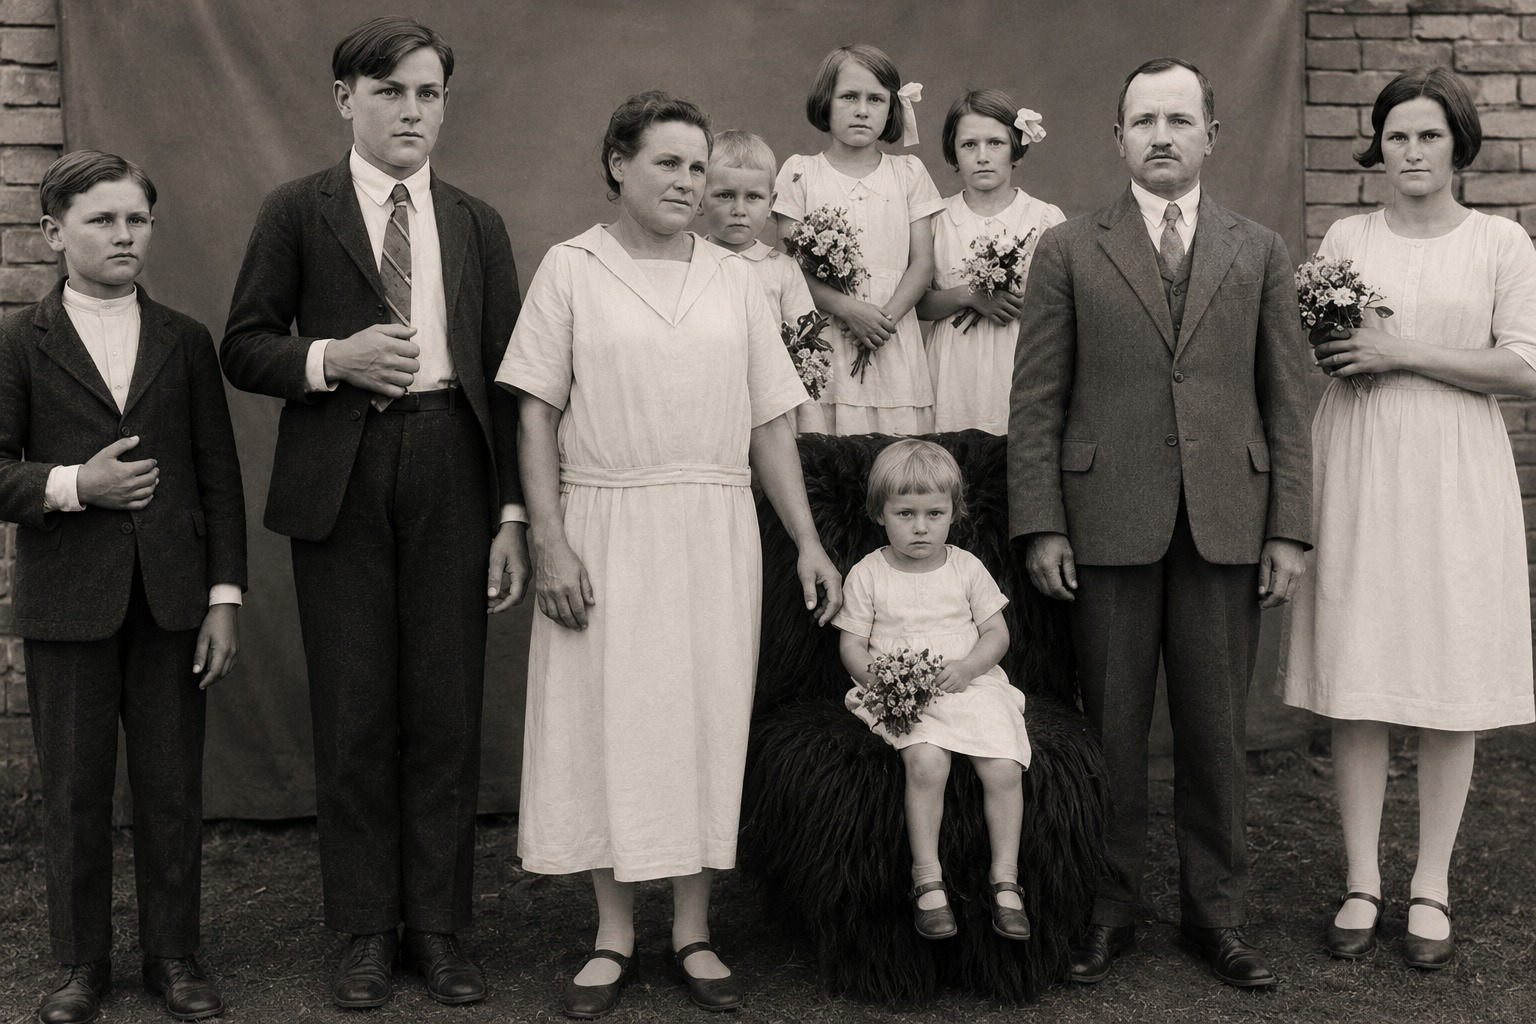
\includegraphics[width=0.85\linewidth,height=\textheight,keepaspectratio,alt={Johann Haas, der Fata (Zweiter von rechts), und Maria Meier Haas, die Mota (in der Mitte, mit dem Baby auf dem Arm), mit den sieben Kindern, die sie in Santa Catarina großzogen. Nach dem sichtbaren Alter der Kinder dürfte das Foto aus der zweiten Hälfte der 1920er-Jahre stammen, schon in Ituporanga; wer welches Kind ist, muss noch mit den Cousins geklärt werden. Familienarchiv. Mit KI restaurierte Fassung; das Original liegt im Repositorium, und Einzelheiten der Gesichter können retuschiert sein.}]{imagens/foto_familia_johann_haas_e_maria_meyer_restaurada.jpg}
\caption{Johann Haas, der \emph{Fata} (Zweiter von rechts), und Maria
Meier Haas, die \emph{Mota\index[pessoas]{meier, maria@Meier, Maria}} (in der Mitte, mit dem Baby auf dem Arm),
mit den sieben Kindern, die sie in Santa Catarina großzogen. Nach dem
sichtbaren Alter der Kinder dürfte das Foto aus der zweiten Hälfte der
1920er-Jahre stammen, schon in Ituporanga\index[lugares]{ituporanga@Ituporanga}; wer welches Kind ist, muss
noch mit den Cousins geklärt werden. Familienarchiv. Mit KI restaurierte
Fassung; das Original liegt im Repositorium, und Einzelheiten der
Gesichter können retuschiert sein.}
\end{figure}

Der Mann mit dem Schnurrbart ist Johann Haas\index[pessoas]{haas, johann@Haas, Johann}, der \emph{Fata}. Die Frau
in der Mitte ist Maria Katharina Meier Haas, die \emph{Mota\index[pessoas]{meier, maria@Meier, Maria}}. Die sieben
Kinder und Jugendlichen sind die Kinder, die sie in Santa Catarina
großzogen: Gertrudes, Fernando, Alexandre, Agnes, Elza, Baldoíno und
Maria. Eines davon ist mein Vater. Das Baby auf dem Arm der Mutter
dürfte die Jüngste sein, Maria, geboren 1926, was die Fotografie auf
etwa 1927 datieren würde; das Kind, das vorne sitzt, könnte mein Vater
sein, mit drei oder vier Jahren, in Weiß gekleidet, wie man damals
kleine Jungen anzuziehen pflegte; es könnte aber auch jemand anderes
sein, und ich will aus einer Vermutung keine Bildunterschrift machen.
Die beiden jungen Männer im Anzug wären Fernando und Alexandre, und die
junge Frau rechts Gertrudes, die Älteste. All das ist aus dem sichtbaren
Alter erschlossen. Ich muss mich noch mit den Cousins zusammensetzen und
Gesicht für Gesicht prüfen.

Was ich mit Sicherheit weiß, ist, was auf der Fotografie fehlt. Es
fehlen Hildegard und Frida, die beiden ersten Töchter, die vor der Reise
in Deutschland starben. Es fehlen Luisa\index[pessoas]{haas, luisa@Haas, Luisa} und Walter, die mit den Eltern
den Ozean überquerten und klein starben; wo, darüber sind sich die
Quellen der Familie nicht einig, und dieser Widerspruch bleibt für das
nächste Kapitel. Und es fehlt João, der noch nicht geboren war und der
ebenfalls klein sterben sollte. Wenn ich dieses Foto betrachte, suche
ich auch nach den Abwesenden.

\section{\texorpdfstring{Der \emph{Fata}}{Der Fata}}\label{der-fata}

Die Enkel nannten ihn \emph{Fata\index[pessoas]{haas, johann@Haas, Johann}}. In meiner Kindheit hielt ich das für
einen Spitznamen, eines jener erfundenen Wörter, die kleine Kinder
benutzen und die die Familie übernimmt. Ich habe lange gebraucht, um zu
verstehen, dass es einfach \emph{Vater} war, so ausgesprochen, wie die
Kinder ihn zu Hause riefen, und mit den brasilianischen Ohren der Enkel
gehört. Genauso bei der \emph{Mota\index[pessoas]{meier, maria@Meier, Maria}}: \emph{Mutter}. In dem Text, den
meine Schwester Marise\index[pessoas]{lourenco, marise haas@Lourenço, Marise Haas} 2013 zum hundertsten Jahrestag der Ankunft
schreiben sollte, verwendet sie beide Formen nebeneinander, \emph{Vater
(Fata\index[pessoas]{haas, johann@Haas, Johann})}, \emph{Mutter (Mota\index[pessoas]{meier, maria@Meier, Maria})}, als würde sie übersetzen und zugleich
bewahren. Die Enkel erbten von den Kindern das Wort für \emph{Vater} und
das Wort für \emph{Mutter} und machten Eigennamen daraus. In keiner
anderen Familie kenne ich Großeltern, die so genannt wurden, und ich
denke gern, dass das etwas über jenes Haus aussagt: Die Kinder sprachen
so viel und so selbstverständlich mit ihren Eltern, dass das gewöhnliche
Wort zum Namen wurde.

Johann Haas\index[pessoas]{haas, johann@Haas, Johann} wurde im Juli 1884 in Bayern\index[lugares]{bayern@Bayern} geboren. Er stammte aus einer
Maurerfamilie und spezialisierte sich auf ein Handwerk, das heute fast
verschwunden ist: die Stuckarbeit. Er machte Fensterumrahmungen,
Portaleinfassungen, Altarornamente, all das, was in den Kirchen und den
reicheren Häusern Europas jener Zeit dem rohen Mauerwerk den letzten
Schliff gab. Es war eine Arbeit, die eine sichere Hand und ein
Künstlerauge verlangte, und er sollte sie in ein Land mitnehmen, in dem
kaum jemand Geld für Ornamente hatte.

In Brasilien rettete ihn diese Fertigkeit mehr als einmal. In den ersten
Jahren, auf trockenem, saurem Boden im Hinterland von Anitápolis\index[lugares]{anitapolis@Anitápolis}, wo der
Ackerbau kaum zum Essen reichte, war es der Gips, der das Brot kaufte:
Er begann, Grabmäler aus Terrazzo für die Friedhöfe der Gegend
herzustellen, verziert mit Mustern und mit von Hand modellierten Engeln.
Später, in Ituporanga\index[lugares]{ituporanga@Ituporanga}, ernährte ihn das Maurerhandwerk, und er brachte
es seinen Söhnen bei. Die Familie baute in der Stadt die Hauptkirche,
das Pfarrhaus, das Franziskanerseminar und die Erweiterung des
Schwesternkrankenhauses. Sie baute auch Häuser, Schulen, Backöfen,
Herde, Treppen und Sägewerke in der ganzen Gegend, nicht immer mit
seinen eigenen Händen, aber mit den Händen derer, die bei ihm gelernt
hatten.

Was in den Erinnerungen aber am häufigsten auftaucht, ist sein Wesen.
\emph{„Unser João war verspielt und lustig: ein Witzbold``}, schrieb
Marise\index[pessoas]{lourenco, marise haas@Lourenço, Marise Haas}. Er ließ keine Gelegenheit aus, etwas Komisches zu sagen. Die
Enkel, die in seinen letzten Jahren in Ribeirão das Pacas\index[lugares]{ribeirao das pacas@Ribeirão das Pacas} mit ihm
zusammenlebten, erzählen, dass sie sich gern in seine Nähe setzten, um
Geschichten zu hören, vor allem wenn er ein paar Bier getrunken hatte,
wenn sich die Zunge löste und Deutschland wieder in den Gesprächen
auftauchte.

Er war auch ein Mann, der las. Das ist ein Detail, das mich rührt,
vielleicht aus Berufskrankheit. Sie waren arme Einwanderer, wie die
meisten, die in die Kolonien kamen, aber, wie es im Text zum hundertsten
Jahrestag heißt, \emph{gebildet}. Sie brachten Bücher aus Deutschland
mit, und diese Bücher wurden im Haus im Wald immer wieder gelesen.
Später hatte die Familie Zeitungen abonniert, vor allem solche aus der
Gegend von Blumenau\index[lugares]{blumenau@Blumenau}, wo die deutschsprachige Presse noch stark war, um
die Nachrichten aus Brasilien und aus dem fernen Land zu verfolgen. Ich
stelle mir den \emph{Fata\index[pessoas]{haas, johann@Haas, Johann}} vor, abends nach einem ganzen Tag auf der
Baustelle, wie er beim Licht der Petroleumlampe eine Woche alte Zeitung
aus Blumenau\index[lugares]{blumenau@Blumenau} liest und nach einer Nachricht aus Bayern\index[lugares]{bayern@Bayern} sucht. Ich weiß
nicht, ob die Szene genau so stattgefunden hat. Ich weiß, dass etwas
Ähnliches oft stattgefunden hat.

Und es gab noch eine Fertigkeit, die ich erst viel später verstand und
die sich als Spur erweisen sollte. Laut dem Text zum hundertsten
Jahrestag wurde Johann häufig als Dolmetscher gerufen, weil er mehrere
deutsche Mundarten beherrschte. Wenn man heute an Deutsch denkt, denkt
man an eine einzige Sprache, die des Radios und der Bücher. Aber das
Deutschland, in dem er geboren wurde, war als Staat erst seit dreizehn
Jahren geeint, und als Sprache war es davon weit entfernt. Ein Bauer aus
Pommern und ein Bauer aus Bayern\index[lugares]{bayern@Bayern} konnten echte Schwierigkeiten haben,
einander zu verstehen. In den brasilianischen Kolonien, wo sich
Einwanderer aus allen Regionen mischten, war jemand, der sich zwischen
diesen Mundarten bewegen konnte, wertvoll. Für den, der forscht, war es
auch ein Zeichen: Der \emph{Fata\index[pessoas]{haas, johann@Haas, Johann}} hatte ein geschultes Ohr für Akzente,
und sein eigener Akzent verriet, woher er kam.

\begin{figure}
\centering
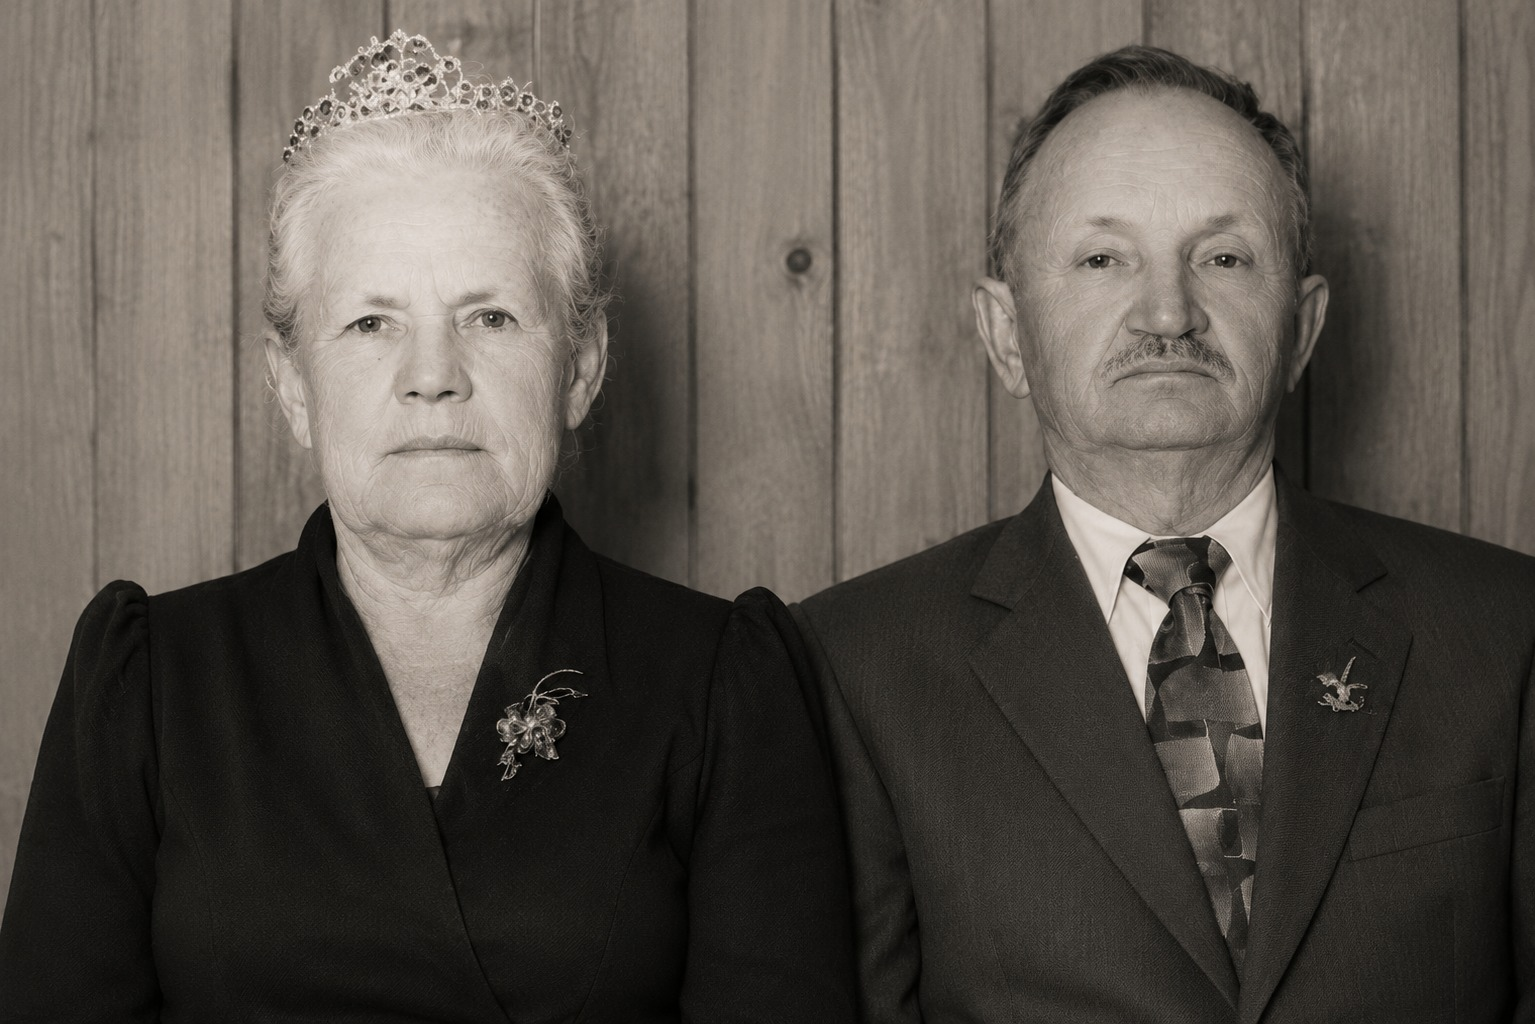
\includegraphics[width=0.75\linewidth,height=\textheight,keepaspectratio,alt={Der Fata und die Mota bei der Goldenen Hochzeit, 1957, wenn man fünfzig Jahre ab der Hochzeit von 1907 rechnet: sie mit einem kleinen Diadem im weißen Haar und einer Blume am dunklen Kleid; er in Anzug und Krawatte, mit einer Anstecknadel am Revers. Familienarchiv. Mit KI restaurierte Fassung; das Original liegt im Repositorium, und Einzelheiten der Gesichter können retuschiert sein.}]{imagens/haas_bodas_de_ouro_fata_e_mota_restaurada.jpg}
\caption{Der \emph{Fata} und die \emph{Mota} bei der Goldenen Hochzeit,
1957, wenn man fünfzig Jahre ab der Hochzeit von 1907 rechnet: sie mit
einem kleinen Diadem im weißen Haar und einer Blume am dunklen Kleid; er
in Anzug und Krawatte, mit einer Anstecknadel am Revers. Familienarchiv.
Mit KI restaurierte Fassung; das Original liegt im Repositorium, und
Einzelheiten der Gesichter können retuschiert sein.}
\end{figure}

\section{\texorpdfstring{Die \emph{Mota}}{Die Mota}}\label{die-mota}

Wenn der \emph{Fata\index[pessoas]{haas, johann@Haas, Johann}} die Stimme des Hauses war, dann war die \emph{Mota\index[pessoas]{meier, maria@Meier, Maria}}
der Boden.

Maria Katharina Meier wurde im April 1888 in Heumaden\index[lugares]{heumaden@Heumaden} in Bayern\index[lugares]{bayern@Bayern} geboren.
Aus welchem Haus sie stammte, erfuhr ich erst viel später. Bevor sie
nach Brasilien aufbrach, verdiente sie neben der Hausarbeit einen Lohn
mit Kühemelken. Nach der Familienüberlieferung war sie es, die sich mit
der Feldarbeit auskannte, und wahrscheinlich war sie der praktische
Rückhalt des ganzen Abenteuers: Der \emph{Fata\index[pessoas]{haas, johann@Haas, Johann}} konnte Mauern bauen,
aber wer wusste, wie man die Erde zum Tragen bringt, die Tiere versorgt
und mitten im Busch einen Haushalt am Laufen hält, das war die
\emph{Mota\index[pessoas]{meier, maria@Meier, Maria}}.

In den Jahren in Rio Novo\index[lugares]{rio novo@Rio Novo}, als die Familie in einem kleinen Haus mitten
im Wald lebte, verbrachte der \emph{Fata\index[pessoas]{haas, johann@Haas, Johann}} tagelang in der Stadt, wo er
als Maurer arbeitete. Die \emph{Mota\index[pessoas]{meier, maria@Meier, Maria}} blieb allein mit den Kindern. Sie
versorgte das Feld, die Tiere, die Kinder und verteidigte sich, in den
Worten des Textes zum hundertsten Jahrestag, so gut sie konnte, den
Blick immer auf den Weg gerichtet, in Erwartung des Mannes, der die
Vorräte brachte, die das Land nicht hergab. In diesem Haus wurden Agnes,
Elza, mein Vater und Maria geboren. Ich denke oft an sie, wenn vom Mut
der Pioniere die Rede ist. Den Mut, sich dem Unbekannten zu stellen,
schreibt man gewöhnlich denen zu, die aufbrechen. Es gibt auch den Mut
derer, die bleiben, allein, auf einer Lichtung, mit vier oder fünf
kleinen Kindern, und den Geräuschen der Nacht lauschen.

Sie hat nie Portugiesisch gelernt. Der Kontakt mit Menschen, die diese
Sprache sprachen, war gering; ihr Leben spielte sich zwischen Haus,
Feld, Familie und Kirche ab, und an all diesen Orten sprach man Deutsch.
Als die Enkel geboren wurden, viele von ihnen schon ohne
Deutschkenntnisse, tat sich zwischen der Großmutter und ihnen eine
Entfernung auf, die keine der beiden Seiten gewählt hatte. Marise\index[pessoas]{lourenco, marise haas@Lourenço, Marise Haas}
erzählt, dass dies die Verständigung sehr erschwerte, die \emph{Mota\index[pessoas]{meier, maria@Meier, Maria}}
aber nicht daran hinderte, das Herz der Enkel mit Blicken, festen Gesten
und dem zu berühren, was sie liebevoll ihr \emph{„Brummeln``} nennt. Ich
mag dieses Wort. Ich stelle mir eine weißhaarige alte Frau vor, die auf
Bairisch vor sich hin brummelt, vor einem Kind, das kein Wort versteht
und trotzdem alles versteht.

In den letzten Jahren, in Ribeirão das Pacas\index[lugares]{ribeirao das pacas@Ribeirão das Pacas}, ging die \emph{Mota\index[pessoas]{meier, maria@Meier, Maria}} auf
Stöcke aus Holzstücken gestützt über das Feld. Die Enkel, die ihr am
nächsten waren, die Kinder von Agnes und Maria, die in der Nähe wohnten,
halfen ihr, sie zu halten. Sie sind es, die die lebendigsten
Erinnerungen an sie bewahren, und sie sind es, die mir in diesem Kapitel
fehlen: Ich muss noch jeden von ihnen in Ruhe anhören, mit
Aufnahmegerät, und um Erlaubnis bitten, das Gesagte zu zitieren. Vorerst
habe ich die Zusammenfassung, die Marise\index[pessoas]{lourenco, marise haas@Lourenço, Marise Haas} aus vielen Stimmen gemacht hat,
und ein Bild, das in allen wiederkehrt. Die \emph{Mota\index[pessoas]{meier, maria@Meier, Maria}} umarmte.
\emph{„Sie ließ keine Gelegenheit aus, zu umarmen, zu umarmen, zu
umarmen``}, schrieb meine Schwester. Und sie hatte blaue Augen, die der
Text \emph{unendlich sanft} nennt.

\begin{figure}
\centering
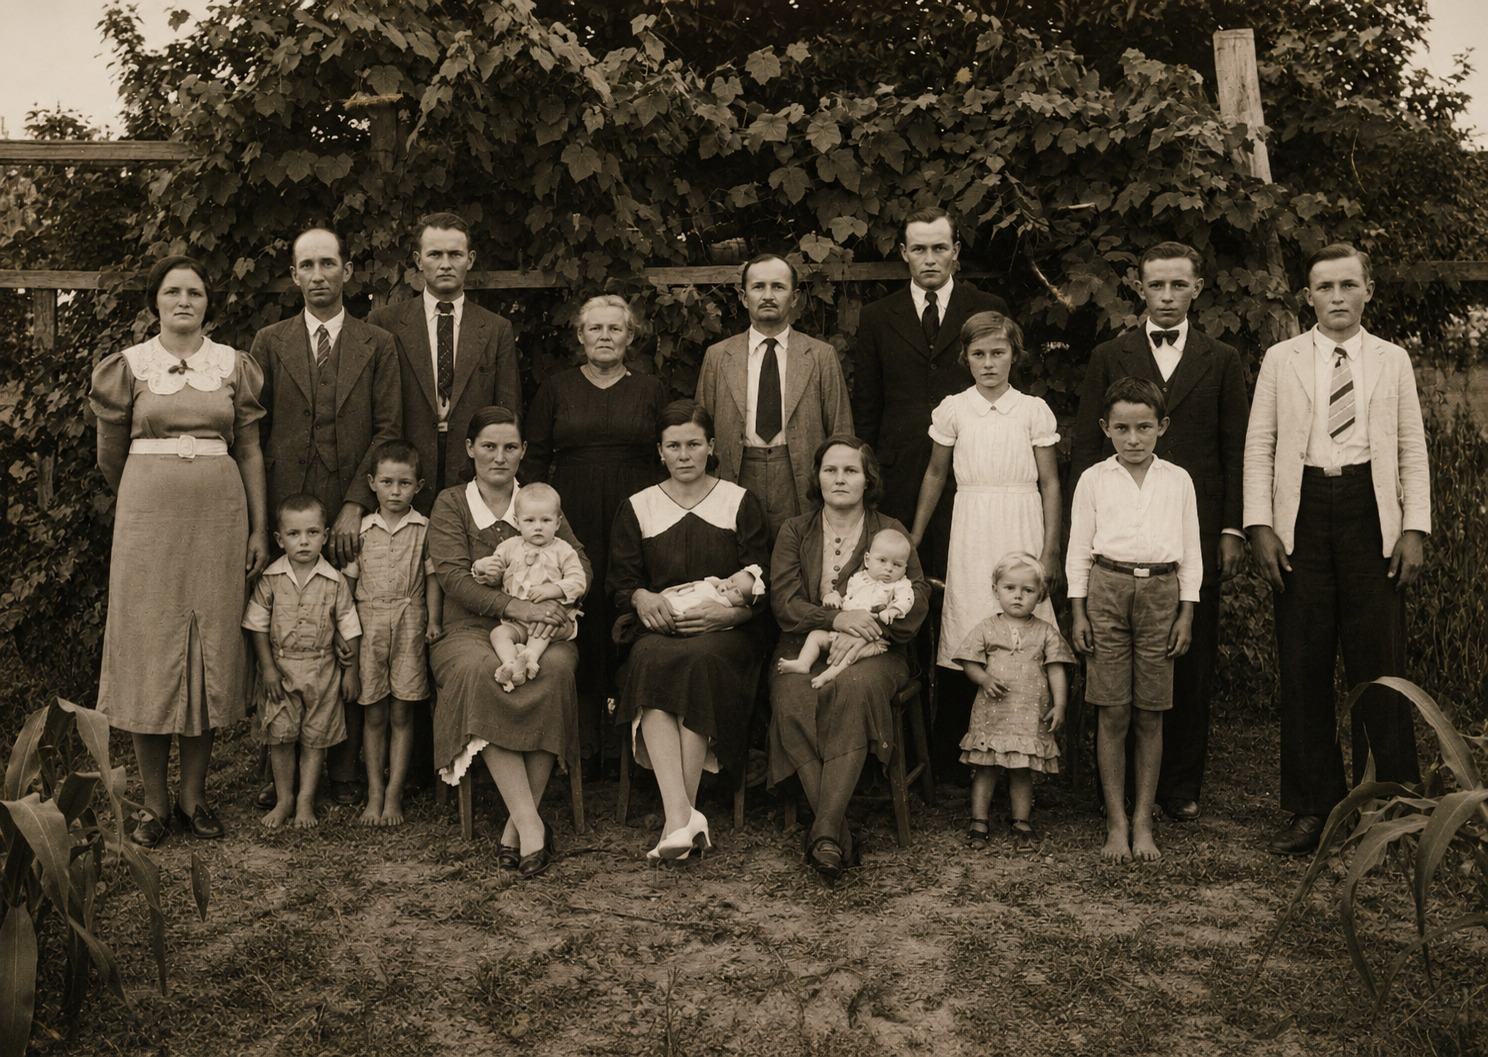
\includegraphics[width=0.85\linewidth,height=\textheight,keepaspectratio,alt={Die ersten Enkel des Fata, mit den Großeltern unter einer Weinlaube versammelt, wahrscheinlich Ende der 1930er-Jahre. Der Fata und die Mota stehen in der Mitte der hinteren Reihe; vorn drei sitzende Mütter mit Babys auf dem Schoß und barfüßige stehende Kinder. Die Zuordnung der einzelnen Personen ist noch zu bestätigen. Familienarchiv. Mit KI restaurierte Fassung; das Original liegt im Repositorium, und Einzelheiten der Gesichter können retuschiert sein.}]{imagens/haas_primeiros_netos_do_fata_restaurada.jpg}
\caption{Die ersten Enkel des \emph{Fata}, mit den Großeltern unter
einer Weinlaube versammelt, wahrscheinlich Ende der 1930er-Jahre. Der
\emph{Fata\index[pessoas]{haas, johann@Haas, Johann}} und die \emph{Mota\index[pessoas]{meier, maria@Meier, Maria}} stehen in der Mitte der hinteren Reihe;
vorn drei sitzende Mütter mit Babys auf dem Schoß und barfüßige stehende
Kinder. Die Zuordnung der einzelnen Personen ist noch zu bestätigen.
Familienarchiv. Mit KI restaurierte Fassung; das Original liegt im
Repositorium, und Einzelheiten der Gesichter können retuschiert sein.}
\end{figure}

Auf dieser anderen Fotografie, die die Familie als das Bild der ersten
Enkel aufbewahrt, erscheint die \emph{Mota\index[pessoas]{meier, maria@Meier, Maria}} in einem dunklen Kleid,
schon mit hellem Haar, stehend inmitten von Söhnen, Töchtern,
Schwiegersöhnen, Schwiegertöchtern und Enkeln, unter einer dicht
belaubten Weinlaube. Sie ist die Einzige, die mit so etwas wie einem
halben Lächeln in die Kamera schaut. Neben ihr, mit dunkler Krawatte,
der \emph{Fata\index[pessoas]{haas, johann@Haas, Johann}}. Die Kinder vorn sind barfuß, wie die Kinder in den
Kolonien gewöhnlich herumliefen, und die Mütter halten die Babys mit der
Selbstverständlichkeit von Menschen, die Übung darin haben. Ich kenne
nicht die Namen aller Personen auf dem Foto und will nichts riskieren.
Ich weiß, dass es ein Erntebild ist: Gut zwanzig Jahre, nachdem sie mit
zwei Kindern, die nicht groß werden sollten, in Brasilien angekommen
waren, standen die beiden da, umgeben von Menschen, die es nur gab, weil
sie geblieben waren.

João Haas starb am 19. März 1969 und Maria am 8. November 1973, beide
mit fünfundachtzig Jahren. Sie sind auf dem Friedhof von Aurora\index[lugares]{aurora@Aurora}
begraben, nahe bei vielen Gräbern, die er selbst gemacht hat.

\section{Zwei Wörter}\label{zwei-wuxf6rter}

Lange Zeit passte alles, was die Familie über die genaue Herkunft der
beiden wusste, in zwei Wörter.

Auf der Seite der \emph{Mota\index[pessoas]{meier, maria@Meier, Maria}} war das Wort \emph{Heumaden\index[lugares]{heumaden@Heumaden}}. Auf der
Seite des \emph{Fata\index[pessoas]{haas, johann@Haas, Johann}} \emph{Sandberg\index[lugares]{sandberg@Sandberg}}, manchmal begleitet von
\emph{Leonberg\index[lugares]{leonberg@Leonberg}}. Es waren Wörter, die mehr gesprochen als geschrieben
wurden, und sie veränderten sich ein wenig, je nachdem, wer sie
aussprach. In der Tabelle, die mein Cousin Agenor\index[pessoas]{haas, agenor@Haas, Agenor} über Jahre
zusammengetragen hat und von der ich im nächsten Kapitel erzählen werde,
erscheint das Dorf der \emph{Mota\index[pessoas]{meier, maria@Meier, Maria}} als \emph{Heimaden} geschrieben, mit
\emph{i}, und Johann erscheint als geboren „in Leonberg\index[lugares]{leonberg@Leonberg}, das heute
Maxhütte heißt und im Bundesland Bayern\index[lugares]{bayern@Bayern} liegt``. Das war viel mehr, als
ich hatte. Es war auch, wie ich herausfinden sollte, ein Minenfeld.

Der Unterschied zwischen \emph{Heumaden\index[lugares]{heumaden@Heumaden}} und \emph{Heimaden} scheint
klein, ein Vokal, aber er sagt viel darüber, wie Namen reisen. Ein Wort,
das neunzig Jahre lang von Mund zu Mund weitergegeben wird, von
Menschen, die die Ursprungssprache nicht mehr sprechen, passt sich
allmählich dem Ohr derer an, die es wiederholen. In \emph{Heumaden\index[lugares]{heumaden@Heumaden}}
steckt das \emph{Heu}, und der Rest des Namens erinnert an die
\emph{Mahd}, und das Dorf ist, so stelle ich mir vor, wohl aus
irgendeiner Heuwiese entstanden, die im Sommer gemäht wurde, um das Vieh
im Winter zu füttern. \emph{Heim} dagegen ist das Zuhause. Ich weiß
nicht, ob der Tausch von dem kam, der zuhörte, oder von dem, der
schrieb, und ich habe keine Möglichkeit, es herauszufinden. Aber ich
finde es schön, dass das Heudorf auf seinem Weg durch das Gedächtnis von
drei brasilianischen Generationen einem Heimatdorf ähnlich geworden ist.

Die Namen der Menschen erlitten denselben Verschleiß. Aus Meier wurde in
vielen brasilianischen Papieren Meyer, und beide Schreibweisen bestehen
bis heute in den Dokumenten der Familie nebeneinander. Aus Johann wurde
João, und Maria bekam im Gedächtnis der Familie ein Katharina dazu, das
im Taufbuch der Name der älteren Schwester war. In der Tabelle erscheint
der Vater der \emph{Mota\index[pessoas]{meier, maria@Meier, Maria}} als Adam Meyer und die Mutter als Franciska
Meyer, mit dem Familiennamen des Mannes, wie man verheiratete Frauen
damals einzutragen pflegte. Jede dieser kleinen Veränderungen ist
harmlos. Zusammengenommen können sie einen Menschen in einem Archiv auf
der anderen Seite des Meeres unkenntlich machen.

Für einen Meteorologen besteht eine Beobachtungsstation aus zwei Dingen:
einer Reihe von Messwerten und einer Position. Die Messwerte allein
nützen nichts. Eine Temperatur von minus zwei Grad um sechs Uhr morgens
ist eine banale Angabe, wenn die Station auf einem Berggipfel steht, und
ein Alarmsignal, wenn sie in einer Küstenniederung steht. Deshalb hat
jede Station Koordinaten: Breite, Länge, Höhe. Und deshalb ist einer der
tückischsten Fehler, die man bei der Datenanalyse machen kann, der
Positionsfehler: ein richtiger Messwert, der dem falschen Ort zugeordnet
wird. Er sieht nicht falsch aus. Die Zahlen sind plausibel, das Format
ist tadellos, nichts fällt auf. Aber sobald er in die Karte eingeht,
verfälscht er alles um sich herum. Das Analyseprogramm passt die
Isolinien an, um diesen Wert unterzubringen, und was ein glattes Feld
sein sollte, bekommt eine seltsame Blase, einen falschen Kälte- oder
Wärmekern, der einen unaufmerksamen Vorhersager davon überzeugen kann,
dass dort etwas ist, wo nichts ist.

Die Ortsnamen in einer Genealogie funktionieren wie die Koordinaten
einer Station. Wenn sie stimmen, fügen sich die Messwerte, die Daten,
die Namen der Eltern, die Berufe, zu einer stimmigen Karte. Wenn sie
falsch sind, wird alles, was danach kommt, auf einem verschobenen Punkt
errichtet. Und die Namen deutscher Dörfer sind besonders tückisch, weil
sie sich wiederholen.

\section{Die Gefahr der
Namensvettern}\label{die-gefahr-der-namensvettern}

Man braucht nur die beiden Wörter in eine Internetkarte einzugeben, um
das Problem zu verstehen.

Leonberg\index[lugares]{leonberg@Leonberg} ist für jeden Deutschen und für die meisten Karten eine Stadt
in Baden-Württemberg, etwa fünfzehn Kilometer westlich von Stuttgart. Es
ist eine bekannte Stadt mit historischer Altstadt, einem Schloss, einer
Rasse riesiger Hunde, die ihren Namen trägt, und einer Autobahn, die
daran vorbeiführt. Wer „Leonberg\index[lugares]{leonberg@Leonberg}, Deutschland`` sucht, landet fast immer
dort. Und Heumaden\index[lugares]{heumaden@Heumaden} gibt es, durch einen Zufall, der wie absichtlich
eingefädelt wirkt, ebenfalls in der Umgebung von Stuttgart: Es ist ein
Stadtteil von Stuttgart selbst, im Bezirk Sillenbuch, etwa zwanzig
Kilometer von Leonberg\index[lugares]{leonberg@Leonberg} entfernt.

Stellt euch die Versuchung vor. Ein brasilianischer Forscher mit zwei
Wörtern, die fast hundert Jahre lang mündlich überliefert wurden, gibt
die beiden Namen ein und entdeckt, dass beide existieren, Seite an
Seite, im selben Ballungsraum im Südwesten Deutschlands. Es sieht aus
wie ein Fund. Es sieht aus wie die Bestätigung, dass die ganze Familie,
\emph{Fata\index[pessoas]{haas, johann@Haas, Johann}} und \emph{Mota\index[pessoas]{meier, maria@Meier, Maria}}, aus derselben Gegend stammte, was erklären
würde, wie die beiden sich kennengelernt hatten. Die Daten sind
plausibel, das Format ist tadellos, nichts fällt auf. Es ist der
Positionsfehler in Reinform.

Ich werde hier nicht behaupten, dass ich in diese Falle getappt bin,
denn ich habe keine Aufzeichnung darüber, und ich will keinen Fehltritt
erfinden, um die Geschichte dramatischer zu machen. Aber ich weiß, dass
sie auf dem Weg aufgestellt war, und ich weiß, dass viele
Familienforscher, in Brasilien und anderswo, schon Monate in
gleichnamigen Städten verloren haben, in Archiven, die nie ein einziges
Papier ihrer Vorfahren aufbewahrt hatten. Die Genealogieforen sind voll
von solchen Geschichten. Deshalb widme ich ihr ein paar Zeilen: damit
ihr, wenn ihr diese Forschung eines Tages fortsetzt, wisst, dass das
erste Ergebnis auf der Karte fast nie das richtige ist.

Es gab mindestens drei Anzeichen dafür, dass die Gegend um Stuttgart
nicht die Antwort war. Das erste stand in Agenors eigener Notiz:
Leonberg\index[lugares]{leonberg@Leonberg}, sagte er, liege in \emph{Bayern\index[lugares]{bayern@Bayern}} und habe seinen Namen in
\emph{Maxhütte} geändert. Das Leonberg\index[lugares]{leonberg@Leonberg} bei Stuttgart war nie bayerisch
und hat auch nie seinen Namen geändert. Das zweite war das Wort
\emph{Sandberg\index[lugares]{sandberg@Sandberg}}, das auf keiner Karte in der Nähe von Stuttgart
auftauchte. Das dritte war der Akzent.

Die Mundarten rund um Stuttgart sind schwäbisch, aus der alemannischen
Familie, verwandt mit den Mundarten der deutschen Schweiz und des
Elsass. Die bayerischen gehören zu einer anderen Familie, der
bairischen, verwandt mit den Mundarten Österreichs. Für ein
brasilianisches Ohr ist das alles Deutsch. Für einen Deutschen ist es
der Unterschied zwischen einem Gaúcho aus dem Grenzland im äußersten
Süden Brasiliens und einem Nordestino aus dem Sertão, dem trockenen
Hinterland des Nordostens, und manchmal mehr. Der Titel dieses Kapitels
spricht von einem bayerischen Akzent und nimmt damit eine
Schlussfolgerung vorweg, die erst die Dokumente später bestätigen
sollten. Aber die Überlegung lag schon bereit: Wenn der \emph{Fata\index[pessoas]{haas, johann@Haas, Johann}}, der
sich zwischen Mundarten bewegte und gerade dafür gerufen wurde, sie
ineinander zu übersetzen, aus Stuttgart gewesen wäre, wäre er mit dem
Schwäbischen aufgewachsen, und die Familie hätte eine andere Melodie von
ihm im Ohr behalten. Und der einzige schriftliche Hinweis, den ich
hatte, Agenors Notiz, sagte klar und deutlich \emph{Bayern\index[lugares]{bayern@Bayern}}.

Wenn man Leonberg\index[lugares]{leonberg@Leonberg} innerhalb Bayerns sucht, taucht etwas anderes auf. In
der Oberpfalz\index[lugares]{oberpfalz@Oberpfalz}, der Region im Nordosten Bayerns, die an Böhmen grenzt,
gut zwanzig Kilometer nördlich von Regensburg\index[lugares]{regensburg@Regensburg}, gibt es eine Gemeinde
namens Maxhütte-Haidhof\index[lugares]{maxhutte-haidhof@Maxhütte-Haidhof}. Der Name kommt von einem Eisenwerk, der
\emph{Maximilianshütte}, die im 19. Jahrhundert gegründet wurde und um
die herum eine Arbeiterstadt wuchs. Leonberg\index[lugares]{leonberg@Leonberg} und Sandberg\index[lugares]{sandberg@Sandberg} sind
Ortsteile, die heute zu dieser Gemeinde gehören. Agenors Notiz stimmte,
und das Wort \emph{Sandberg\index[lugares]{sandberg@Sandberg}} passte: Es war der Name eines kleinen
Ortes, der mit Leonberg\index[lugares]{leonberg@Leonberg} verbunden war, neben dem Eisenwerk, und der Ort,
an dem, allem Anschein nach, Johanns Familie gelebt hatte.

Und Heumaden\index[lugares]{heumaden@Heumaden}? Das gibt es ebenfalls in der Oberpfalz\index[lugares]{oberpfalz@Oberpfalz}. Es ist ein kleines
Dorf der Gemeinde Moosbach\index[lugares]{moosbach@Moosbach} im Landkreis Neustadt an der Waldnaab, keine
zwanzig Kilometer von der heutigen Grenze zur Tschechischen Republik
entfernt, in einer Gegend mit Hügeln, Wäldern und kleinen Bauernorten.
Es liegt etwa fünfzig Kilometer Luftlinie von Maxhütte-Haidhof\index[lugares]{maxhutte-haidhof@Maxhütte-Haidhof} entfernt
und mehr als zweihundert von Stuttgart. Die zuständige Pfarrei ist
St.~Peter und Paul in Moosbach\index[lugares]{moosbach@Moosbach}.

Ich trug die beiden Punkte auf der Karte ein, wie ich zwei Stationen
eintragen würde. Zwei Dörfer derselben Region, getrennt durch eine
Entfernung, die man zu Fuß in zwei Tagen oder mit der Bahn in wenigen
Stunden zurücklegte, beide in der Oberpfalz\index[lugares]{oberpfalz@Oberpfalz}, beide mit derselben
Mundart. Plötzlich hörten die beiden Wörter auf, Legenden zu sein, und
wurden zu Koordinaten: Heumaden\index[lugares]{heumaden@Heumaden}, etwa 49,6° nördlicher Breite und 12,4°
östlicher Länge; Leonberg\index[lugares]{leonberg@Leonberg}, in Maxhütte-Haidhof\index[lugares]{maxhutte-haidhof@Maxhütte-Haidhof}, etwa 49,2° Nord und
12,1° Ost.

Aber in Agenors Notiz gab es ein drittes Wort, das zu nichts davon
passte. Ihm zufolge hatten Johann und Maria am 3. August 1907 in
\emph{Eibenstock\index[lugares]{eibenstock@Eibenstock}} geheiratet. Eibenstock, wenn es die Stadt ist, die die
Karten zeigen, liegt nicht in Bayern\index[lugares]{bayern@Bayern}. Es liegt in Sachsen\index[lugares]{sachsen@Sachsen}, im
Erzgebirge, an der tschechischen Grenze, ein gutes Stück weiter
nördlich. Was hätten ein Stuckateur aus Leonberg\index[lugares]{leonberg@Leonberg} und eine junge Frau aus
Heumaden\index[lugares]{heumaden@Heumaden} dort zu suchen gehabt? Arbeit vielleicht. Eine Baustelle, eine
Saison, ein Verwandter. Oder vielleicht ist es ein weiterer
Namensvetter, eine weitere verschobene Station. Ich weiß es nicht. Ich
lasse den Punkt mit einem Fragezeichen auf der Karte stehen, und so geht
man mit einem verdächtigen Wert um: Man löscht ihn nicht, aber man
vertraut ihm auch nicht, bevor man ihn überprüft hat.

Ich hatte jetzt zwei wirkliche Dörfer anstelle von zwei Wörtern, ein
Hochzeitsdatum an einem rätselhaften Ort und eine Handvoll Fragen, die
kein Familiengespräch beantworten würde: wo die Geburtseinträge zu
finden wären, wer die Eltern von Johann und Maria waren, ob Geschwister
in Bayern\index[lugares]{bayern@Bayern} geblieben waren, ob jemand auf der anderen Seite noch
denselben Familiennamen trug.

Es waren zu große Fragen für einen einzelnen Mann mit einem Computer und
ein paar freien Abenden pro Woche. Die gute Nachricht war, dass ich
nicht allein war. In der Familie gab es, über ganz Brasilien verstreut,
andere Neugierige, die seit Jahren Teile sammelten, jeder mit seinem
Stück des Puzzles und keiner mit dem vollständigen Bild.

\section{Für euch zum Entdecken}\label{fuxfcr-euch-zum-entdecken-1}

\begin{itemize}
\tightlist
\item
  Welches der Kinder auf der Fotografie mit den neun Gesichtern ist
  Baldoíno? Setzt euch mit den Cousins zusammen und prüft Gesicht für
  Gesicht.
\item
  Ist das Eibenstock\index[lugares]{eibenstock@Eibenstock} aus Agenors Notiz wirklich die Stadt in Sachsen\index[lugares]{sachsen@Sachsen},
  oder ist es ein weiterer Namensvetter? Und was hätten ein Stuckateur
  aus Leonberg\index[lugares]{leonberg@Leonberg} und eine junge Frau aus Heumaden\index[lugares]{heumaden@Heumaden} dort zu suchen gehabt?
\item
  Kam der Tausch von \emph{Heumaden\index[lugares]{heumaden@Heumaden}} zu \emph{Heimaden} von dem, der
  zuhörte, oder von dem, der schrieb?
\item
  Was sagte die \emph{Mota\index[pessoas]{meier, maria@Meier, Maria}} in ihrem „Brummeln``? Fragt die Enkel, die
  in Ribeirão das Pacas\index[lugares]{ribeirao das pacas@Ribeirão das Pacas} in ihrer Nähe wohnten, die Kinder von Agnes und
  Maria.
\end{itemize}

\chapter{Die Bruderschaft der Detektiv-Cousins}\label{cap-3}

\emph{27,6° S · 48,5° W, Florianópolis\index[lugares]{florianopolis@Florianópolis}, SC}

\begin{quote}
\emph{Kein Beobachter sieht das ganze Gewitter. Das Netz sieht es.}
\end{quote}

Zwei ernsthafte Menschen aus der Familie haben die Geschichte desselben
Mädchens aufgeschrieben, und sie sind sich weder über das Jahr noch über
den Kontinent ihrer Geburt einig. Nach meiner Schwester wurde Gertrudes,
die Schwester meines Vaters, am 5. Mai 1913 in der Einwandererbaracke
von Laguna\index[lugares]{laguna@Laguna} geboren. Nach einem Cousin wurde sie am 22. Oktober 1911
geboren, noch in Deutschland, und kam mit einem Jahr auf der
\emph{Formosa} herüber. Auf diesen Widerspruch bin ich nach und nach
gestoßen.

\section{Hundert Jahre später}\label{hundert-jahre-spuxe4ter}

Am 30. März 2013 kamen die Nachkommen von João und Maria Meyer Haas
zusammen, um den hundertsten Jahrestag ihrer Ankunft in Brasilien zu
feiern. Wir waren, nach der Zählung, die man damals machte, mehr als
sechshundert direkte Nachkommen, verstreut über Santa Catarina, Paraná
und andere Winkel des Landes und der Welt. Ein guter Teil davon war
dort.

Ich werde das Fest nicht rekonstruieren. Ich habe keine Notizen von
jenem Tag, und die Bilder, die in der Erinnerung umgehen, sind zu vage,
um daraus eine Szene zu machen, ohne am Ende etwas zu erfinden. Was mir
vom hundertsten Jahrestag geblieben ist, ist ein Text. Meine jüngere
Schwester, Marise\index[pessoas]{lourenco, marise haas@Lourenço, Marise Haas} Haas Lourenço, schrieb an jenem Tag eine Geschichte
von João und Maria und las sie vor, unterzeichnet mit „Florianópolis\index[lugares]{florianopolis@Florianópolis},
März 2013``. Dieser Text ist bis heute die vollständigste Quelle, die
die Familie über die beiden besitzt, und ein guter Teil von Teil II
dieses Buches stützt sich darauf.

\begin{ficha}

\textbf{Archivkarte}: \emph{Geschichte von João und Maria Meyer Haas},
Text von Marise\index[pessoas]{lourenco, marise haas@Lourenço, Marise Haas} Haas Lourenço, vorgelesen zum hundertsten Jahrestag der
Ankunft (30.03.2013), unterzeichnet mit „Florianópolis\index[lugares]{florianopolis@Florianópolis}, März 2013``.
Digitale Kopie im Repositorium der Familie:
\texttt{livro/fontes/historia\_joao\_e\_maria\_marise\_2013.txt}. Von
der Autorin angegebene Quellen: Dokumente und Fotos; Recherchen in
Archiven, Museen und Bibliotheken; Interviews; Erzählungen.

\end{ficha}

Ich habe diesen Text nach jenem Tag oft gelesen, und jede Lektüre zeigte
mir etwas anderes. Beim ersten Mal las ich ihn als Enkel: eine
bewegende, gut erzählte Geschichte, mit Verlusten und Errungenschaften,
mit dem Mut der Großeltern und der Dankbarkeit der Nachkommen. Beim
zweiten Mal las ich ihn als Forscher und begann zu unterstreichen. Beim
dritten Mal las ich ihn als Meteorologe und merkte, dass der Text selbst
das Ergebnis eines Netzes war.

Marise\index[pessoas]{lourenco, marise haas@Lourenço, Marise Haas} beginnt mit einer Erklärung zur Methode, die ich gern selbst
geschrieben hätte. Sie sagt, viele hätten dazu beigetragen, dass die
Geschichte geschrieben werden konnte, und um niemanden zu vergessen,
nenne sie lieber gar keinen Namen. Sie sagt, der Text \emph{„entspringt
nicht dem Kopf der Person, die ihn geschrieben hat``}, sondern versuche,
der Wahrheit so nahe wie möglich zu kommen. Und sie zählt die Quellen
auf: Dokumente und Fotos, Recherchen in Archiven, Museen und
Bibliotheken, Interviews, Erzählungen. Darin steckt, ohne dass sie das
Wort benutzt, die genaue Beschreibung einer Synthesearbeit: viele
Teilbeobachtungen von ungleicher Qualität, zu einem einzigen Bild
zusammengefügt.

Gleich danach macht sie eine Bemerkung, die mir damals nur wie eine
Höflichkeit vorkam und die ich heute für den wichtigsten Satz des Textes
halte. Die Familie Haas, schreibt sie, \emph{„ist kein Familienname``},
sondern die Gesamtheit unzähliger anderer, ohne die es keine Familie
gibt. Und sie dankt einigen davon namentlich: den Meyers, der Familie
der \emph{Mota\index[pessoas]{meier, maria@Meier, Maria}}; den Sebolds, der Familie von Onkel Augusto; den da
Rosas, der Familie von Tante Rosalina; den Klettenbergs, der Familie von
Tante Paula; den Boeings, der Familie von Onkel João; den Nagels, der
Familie von Onkel Paulo; den Doerners, der Familie von Tante Adelina,
die meine Mutter war; und den Sautners, der Familie von Onkel Martin\index[pessoas]{sautner, martin@Sautner, Martin}.
Und damit allen anderen Familiennamen, ohne die jene Familie von mehr
als sechshundert Menschen nicht existieren würde.

Wie genau diese Liste war, verstand ich erst Monate später, als ich sie
mit einer anderen Quelle verglich. Aber schon beim ersten Lesen berührte
sie mich aus einem anderen Grund. Ich hatte jahrelang an meine
Genealogie als an eine Linie gedacht, die Haas-Linie, die von mir zu
meinem Vater hinaufstieg, von meinem Vater zum \emph{Fata\index[pessoas]{haas, johann@Haas, Johann}}, vom
\emph{Fata\index[pessoas]{haas, johann@Haas, Johann}} nach Bayern\index[lugares]{bayern@Bayern}. Marise\index[pessoas]{lourenco, marise haas@Lourenço, Marise Haas} sagte, mit aller Behutsamkeit, dass
diese Linie nicht für sich allein existierte. Dass jede Generation aus
der Begegnung zweier Familien entstanden war und dass die Hälfte, die
nicht den Familiennamen trug, für das Ergebnis genauso verantwortlich
war wie die andere. Es war dasselbe, was ich am Tisch in Vidal Ramos\index[lugares]{vidal ramos@Vidal Ramos}
gesehen hatte, zwischen den Haas meines Vaters und den Doerners meiner
Mutter. Jetzt stand es geschrieben.

\begin{figure}
\centering
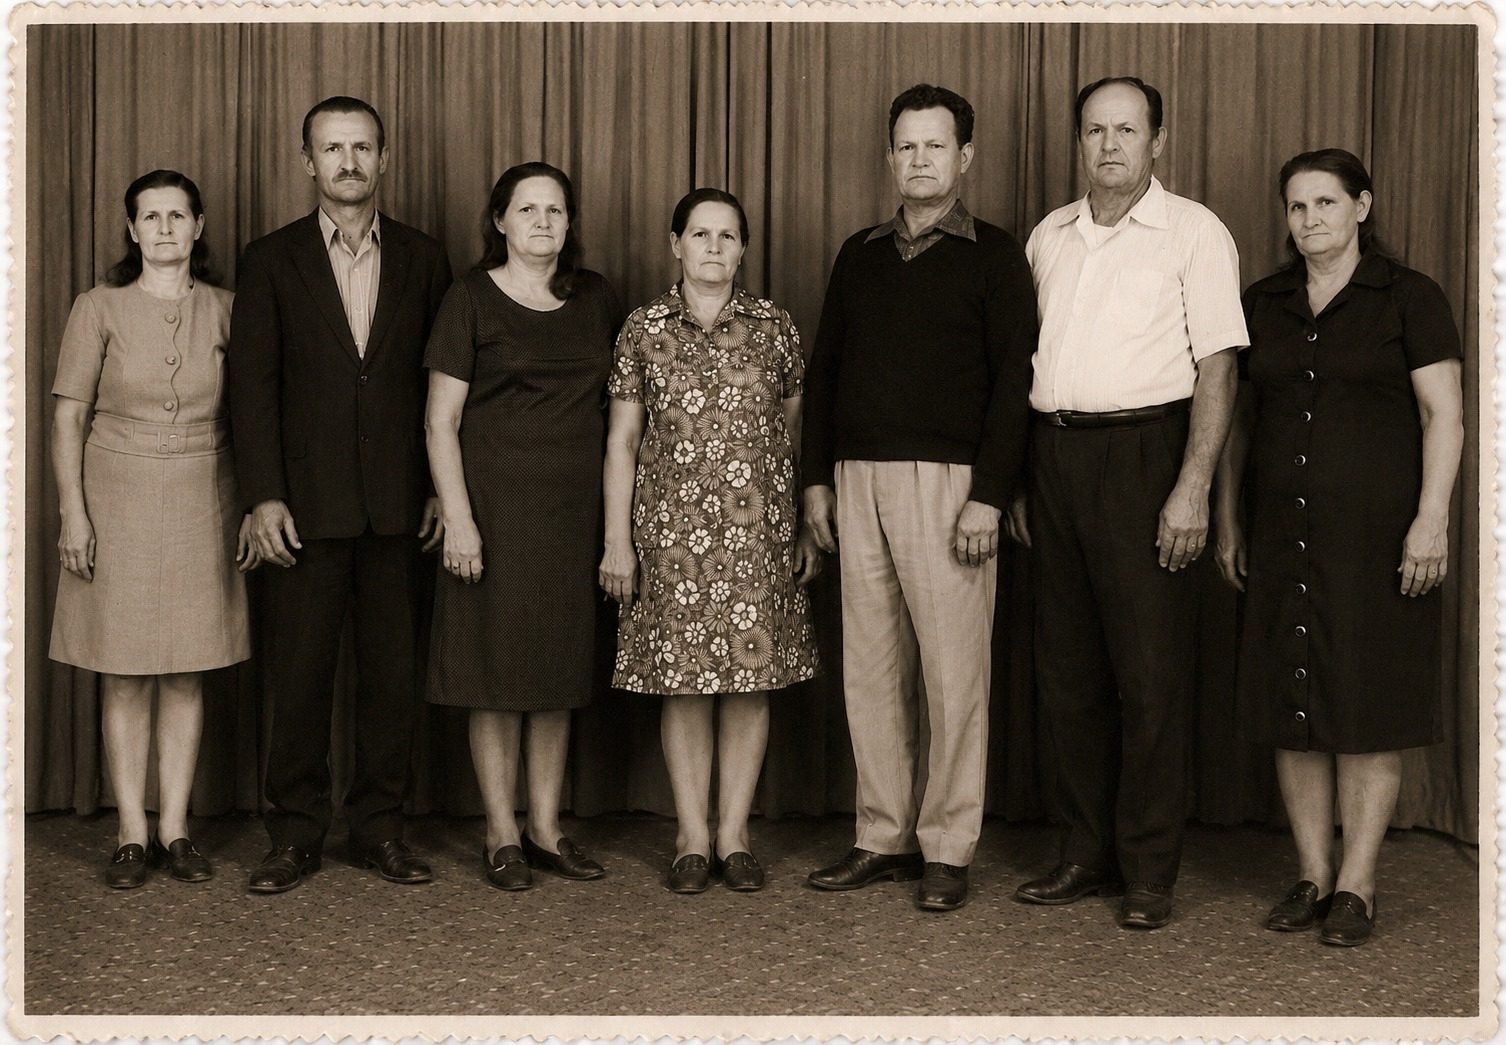
\includegraphics[width=0.85\linewidth,height=\textheight,keepaspectratio,alt={Die Haas-Geschwister, versammelt zu einem Studioporträt vor einem Vorhang: vier Frauen und drei Männer im reiferen Alter, die sieben Kinder von Johann und Maria, die das Erwachsenenalter erreichten, darunter Baldoíno, mein Vater. Das Datum und die Position jedes Geschwisters auf dem Foto sind noch zu vermerken. Familienarchiv. Mit KI restaurierte Fassung; das Original liegt im Repositorium, und Einzelheiten der Gesichter können retuschiert sein.}]{imagens/haas_irmaos_reunidos_restaurada.jpg}
\caption{Die Haas-Geschwister, versammelt zu einem Studioporträt vor
einem Vorhang: vier Frauen und drei Männer im reiferen Alter, die sieben
Kinder von Johann und Maria, die das Erwachsenenalter erreichten,
darunter Baldoíno, mein Vater. Das Datum und die Position jedes
Geschwisters auf dem Foto sind noch zu vermerken. Familienarchiv. Mit KI
restaurierte Fassung; das Original liegt im Repositorium, und
Einzelheiten der Gesichter können retuschiert sein.}
\end{figure}

\section{Der Text und was er nicht
sagt}\label{der-text-und-was-er-nicht-sagt}

Marises Text erzählt die Geschichte der Reihe nach. Die Hochzeit 1907,
noch in jungen Jahren. Johanns Handwerk, aus einer Maurerfamilie,
Fachmann für Stuck, Dolmetscher zwischen Mundarten. Marias Arbeit, die
gegen Lohn Kühe molk. Die Krise in Deutschland, die Kriegsgefahr, der
frühe Tod der beiden ersten Töchter, Hildegard und Frida, \emph{„aus
Gründen, die wir nicht kennen``}. Die Geburt von Luisa\index[pessoas]{haas, luisa@Haas, Luisa} 1910 und von
Walter 1912. Die Entscheidung aufzubrechen, getroffen, so stellt sie es
sich vor, nach vielen Gesprächen und vielen Meinungen dafür und dagegen.
Die Einschiffung auf der \emph{Formosa} in Marseille\index[lugares]{marseille@Marseille}, mit der
schwangeren Maria und den beiden Kleinen auf dem Arm.

Dann die Ankunft. Der Text sagt, das Schiff sei am 26. März 1913 in
Brasilien angekommen, die Ausschiffung in Rio de Janeiro\index[lugares]{rio de janeiro@Rio de Janeiro} sei verweigert
worden, und der Dampfer sei von Hafen zu Hafen die Küste
entlanggefahren, unter Quarantäne, mit zu vielen Passagieren, schlechtem
Essen und mangelhafter Hygiene, und mit vielen Toten an Bord. Die
Familie sei schließlich in Laguna\index[lugares]{laguna@Laguna} an Land gegangen, in die
Einwandererbaracke gebracht worden, und dort sei sechs Tage später, am
5. Mai, Gertrudes geboren worden. Luisa\index[pessoas]{haas, luisa@Haas, Luisa} und Walter, von der Reise
geschwächt, hätten es nicht überstanden. Fast nichts davon, so sollte
ich später herausfinden, hält den Dokumenten stand.

Von da an führt die Geschichte zum Lote 17, dem Landlos Nr. 17, in Rio
do Ouro, heute Anitápolis\index[lugares]{anitapolis@Anitápolis}, nach Ituporanga\index[lugares]{ituporanga@Ituporanga}, Rio Novo\index[lugares]{rio novo@Rio Novo}, Águas Negras\index[lugares]{aguas negras@Águas Negras}, zu
den Bauten der Stadt, zum Krieg, zum Radio im Keller, zum Alter in
Ribeirão das Pacas\index[lugares]{ribeirao das pacas@Ribeirão das Pacas} und zu den Gräbern in Aurora\index[lugares]{aurora@Aurora}. Marise\index[pessoas]{lourenco, marise haas@Lourenço, Marise Haas} verschweigt die
harten Teile nicht. Sie spricht von der Politik der Landnahme auf
indigenem Gebiet und von den Bugreiros, den Indianerjägern, die pro Kopf
bezahlt wurden, und nennt das beim Namen, den es verdient: ein vom Staat
geförderter Völkermord. Sie spricht von den Nachrichten über Gewalt
gegen Deutschstämmige während des Krieges, die die Familie erreichten
und den \emph{Fata\index[pessoas]{haas, johann@Haas, Johann}} dazu brachten, das Gewehr geladen in Reichweite zu
halten. Und sie endet mit einer Frage, die sie selbst beantwortet:
\emph{„Klingt das nach einer traurigen Geschichte? Nein, traurig ist sie
nicht.``}

Als Enkel stimmte ich zu. Als Forscher begann ich Fragen zu stellen, die
der Text nicht beantwortete und auch nicht beantworten musste. An
welchem Tag genau verließen sie Deutschland? Wurde die Ausschiffung in
Rio wirklich verweigert? Gab es eine Quarantäne? In welchem Hafen von
Santa Catarina gingen sie an Land? Wo wurden Luisa\index[pessoas]{haas, luisa@Haas, Luisa} und Walter begraben?
Wenn Gertrudes in der Baracke von Laguna\index[lugares]{laguna@Laguna} geboren wurde, gibt es dann
einen Taufeintrag in der Pfarrei? Und woher in Deutschland kamen die
beiden? Der Text nennt kein einziges Dorf.

Ein Text, der geschrieben wurde, um bei einer Hundertjahrfeier vor
sechshundert Menschen vorgelesen zu werden, ist nicht der Ort für
Fußnoten. Es waren Fragen, die nur andere Dokumente beantworten konnten,
und ich wusste, dass einige dieser Dokumente schon in den Händen von
jemandem aus der Familie waren.

\section{Die Tabelle aus Londrina}\label{die-tabelle-aus-londrina}

Dieser Jemand war mein Cousin ersten Grades Agenor\index[pessoas]{haas, agenor@Haas, Agenor} Haas.

Agenor\index[pessoas]{haas, agenor@Haas, Agenor} wurde 1943 in Ituporanga\index[lugares]{ituporanga@Ituporanga} geboren, als ältester Sohn von Alexandre
Haas und Paula Klettenberg, was ihn auf demselben Weg wie mich zum Enkel
des \emph{Fata\index[pessoas]{haas, johann@Haas, Johann}} und der \emph{Mota\index[pessoas]{meier, maria@Meier, Maria}} macht, nur zweiundzwanzig Jahre
früher. Er ist Bauingenieur, Absolvent der Bundesuniversität von Paraná,
hat sein Leben der Ausführung von Bauprojekten gewidmet und lebt seit
vielen Jahren in Londrina. Jahrelang hat er, ohne Aufhebens, mit der
Geduld eines Ingenieurs und der Methode eines Menschen, der an
Kostenvoranschläge und Zeitpläne gewöhnt ist, eine Tabelle mit allen
Nachkommen von Johann und Maria angelegt, die er finden konnte.

Als die Tabelle bei mir ankam, in einem der vielen Nachrichtenwechsel,
die wir hatten, brauchte ich eine Weile, um zu begreifen, wie groß das
war, was da vor mir lag. Es sind 291 Zeilen. In der ersten Spalte die
Kinder von Johann und Maria und ihre Ehepartner; in der zweiten die
Enkel; in der dritten die Urenkel; in der vierten die Ururenkel. Nach
der Zusammenfassung, die der Tabelle beiliegt, sind es 11 Kinder, 63
Enkel, 194 Urenkel und 109 Ururenkel. In vielen Zellen stehen
Kommentare, Agenors Notizen, insgesamt 55, mit Daten, Orten, Berufen und
kleinen Biografien.

Eines der ersten Dinge, die mir auffielen, war, dass die meisten dieser
Notizen den Computer nicht verlassen durften. Agenor\index[pessoas]{haas, agenor@Haas, Agenor} hatte gesammelt,
was die Familie ihm schickte, und die Familie schickte alles:
vollständige Anschriften, Telefonnummern, E-Mail-Adressen, Schulbildung,
Beruf, Familienstand, Namen von Kindern. Es war ein kostbares Porträt
einer Familie zu einem bestimmten Zeitpunkt zu Beginn des 21.
Jahrhunderts, und es war auch eine Sammlung persönlicher Daten lebender
Menschen, die ihrer Veröffentlichung nie zugestimmt haben. Deshalb kommt
keine dieser Angaben in dieses Buch. Über die lebenden Nachkommen
spreche ich nur in Zahlen. Von den Notizen verwende ich nur die, die die
Stammeltern und die Kinder von Johann und Maria betreffen, die alle
schon verstorben sind oder zu den Gestalten der Familiengeschichte
gehören. Wenn eines Tages ein Cousin seine eigene Geschichte erzählen
will, soll er sie mit seiner eigenen Stimme erzählen.

Die Notizen zu den Stammeltern aber waren Gold wert.

In Johanns Zelle schrieb Agenor\index[pessoas]{haas, agenor@Haas, Agenor} eine kleine Zusammenfassung seines
Lebens. Dort steht, er sei Maurer gewesen, Deutscher, geboren in
Leonberg\index[lugares]{leonberg@Leonberg}, \emph{„das heute Maxhütte heißt``}, in Bayern\index[lugares]{bayern@Bayern}, Sohn von Josef
Haas und Franziska. Er habe am 3. August 1907 in Eibenstock\index[lugares]{eibenstock@Eibenstock} geheiratet.
Er habe Deutschland am 13. März 1913 verlassen und sei am 26. April nach
44 Tagen Reise auf dem Schiff \emph{Formosa} in Rio de Janeiro\index[lugares]{rio de janeiro@Rio de Janeiro}
angekommen. In seinen Worten: \emph{„Die Eintragung ihrer Ausschiffung
in Florianópolis\index[lugares]{florianopolis@Florianópolis} wurde noch nicht gefunden.``} Er habe bis 1918 in Rio
do Ouro gelebt, dann in Rio Novo\index[lugares]{rio novo@Rio Novo}, dann in der Stadt Ituporanga\index[lugares]{ituporanga@Ituporanga}, wieder
in Rio Novo\index[lugares]{rio novo@Rio Novo}, ab 1930 in Águas Negras\index[lugares]{aguas negras@Águas Negras} und schließlich in Rio das Pacas,
Aurora\index[lugares]{aurora@Aurora}, wo er am 19. März 1969 starb. In Marias Zelle steht, sie sei am
7. April 1888 in \emph{Heimaden} geboren, Tochter von Adam und Franciska
Meyer, und am 8. November 1973 gestorben.

Es war das erste Mal, dass ich die Namen von Johanns Eltern schriftlich
sah. Es war das erste Mal, dass ich ein Hochzeitsdatum sah. Es war das
erste Mal, dass ich das Wort \emph{Maxhütte} sah. Und es war, wie ich
bald merkte, auch das erste Mal, dass ich die Geschichte anders erzählt
sah als in Marises Text.

\section{Wenn die Quellen sich
widersprechen}\label{wenn-die-quellen-sich-widersprechen}

Ich legte die beiden Fassungen nebeneinander, wie ich es tue, wenn ich
zwei Reanalysen desselben Sturms vergleiche. Wenn zwei Modelle
übereinstimmen, atmet man auf. Wenn sie sich widersprechen, beginnt die
interessante Arbeit, denn der Unterschied zwischen ihnen zeigt
gewöhnlich genau auf die Stelle, an der die Daten am dürftigsten sind.

Die Widersprüche zeigten sich sofort.

Der erste betraf Johanns Geburtsdatum. Agenor\index[pessoas]{haas, agenor@Haas, Agenor} schrieb 8. Juli 1884. Das
Datum, das ich heute für sicher halte, ist ein anderes und stammt aus
einem Dokument, von dem ich erst an seiner Stelle erzähle. Der
Unterschied ist klein, nur wenige Tage, aber in einer genealogischen
Untersuchung können wenige Tage den Unterschied ausmachen zwischen dem
Finden und dem Nichtfinden eines Eintrags in einem Standesamtsregister.
Damals konnte ich noch nicht wissen, welches der beiden Daten stimmte.

Der zweite betraf das Datum der Abreise. Agenor\index[pessoas]{haas, agenor@Haas, Agenor} sagte 13. März 1913. Die
Familie bewahrt eine Fotografie auf, die vor der Reise aufgenommen
wurde, mit einer deutschen Inschrift auf der Rückseite: \emph{„Zum
Andenken! vor unserer Abreise nach Brasilien, 7. März 1913``}. Ein
Abschiedsfoto kann einige Tage vor der Einschiffung gemacht worden sein,
und die beiden Daten schließen sich nicht unbedingt aus. Aber sie waren
ein weiteres Teil, das eingepasst werden musste.

Der dritte betraf die Ankunft. Marise\index[pessoas]{lourenco, marise haas@Lourenço, Marise Haas} sprach vom 26. März 1913 in Rio de
Janeiro. Agenor\index[pessoas]{haas, agenor@Haas, Agenor} sprach vom 26. April und rechnete nach: 44 Tage Reise.
Ich machte dieselbe Rechnung, und sie geht auf: Vom 13. März bis zum 26.
April sind es tatsächlich 44 Tage. Agenors Notiz war in sich stimmig.
Nur war der Tag derselbe, der 26., und der Monat ein anderer. Das hatte
ganz den Anschein eines einzigen Versehens, eines vertauschten Monats
auf irgendeinem Papier irgendwann im Lauf der Überlieferung, das sich
dann in die Berechnung der Tage fortgepflanzt hatte. Es war, als fände
man in einer Datenreihe einen Wert, der vollkommen zu seinen Nachbarn
passt, bis auf eine Ziffer.

Der vierte war der schwerwiegendste, und er betraf Gertrudes. Nach dem
Text zum hundertsten Jahrestag wurde sie am 5. Mai 1913 in der
Einwandererbaracke von Laguna\index[lugares]{laguna@Laguna} geboren, sechs Tage nach der Ausschiffung:
Sie war das Kind, das Maria während der Reise im Leib trug. Nach Agenors
Tabelle wurde Gertrudes am 22. Oktober 1911 geboren, noch in
Deutschland, und kam mit einem Jahr auf der \emph{Formosa} herüber.

Der fünfte hing mit dem vierten zusammen. In Marises Text hießen die
beiden Kinder, die nach der Ankunft starben, Luisa\index[pessoas]{haas, luisa@Haas, Luisa} und Walter, 1910 und
1912 in Deutschland geboren, und sie starben in Laguna\index[lugares]{laguna@Laguna}. In Agenors
Tabelle gibt es weder Luisa\index[pessoas]{haas, luisa@Haas, Luisa} noch Walter. Stattdessen gibt es eine Lina
und einen Valter, die in Brasilien, in Rio do Ouro\index[lugares]{rio do ouro@Rio do Ouro}, geboren und klein
gestorben sein sollen, begraben in Anitápolis\index[lugares]{anitapolis@Anitápolis}. In der Tabelle stehen die
beiden zwischen Alexandre, Jahrgang 1917, und Agnes, Jahrgang 1920, als
wären sie in diesem Zeitraum geboren. Es gibt sogar ein merkwürdiges
Detail: In Valters Notiz heißt es, er \emph{„starb, als sie noch klein
war``}, in der weiblichen Form, als wäre der Satz aus Linas Notiz
kopiert und nicht berichtigt worden.

Schließlich war da Eibenstock\index[lugares]{eibenstock@Eibenstock}, der Ort der Hochzeit, der weder in der
Nähe von Leonberg\index[lugares]{leonberg@Leonberg} noch in der Nähe von Heumaden\index[lugares]{heumaden@Heumaden} lag. Und es gab ein
Detail bei der Zählung. Die Zusammenfassung spricht von elf Kindern;
aber als ich die erste Spalte Zeile für Zeile durchging, fand ich zwölf
Namen, weil der kleine João, der Jüngste, der als Kind starb, allein
gegen Ende der Tabelle auftaucht. Nach Marises Text kommt man ebenfalls
auf zwölf: die vier verlorenen Kinder, die sieben, die groß wurden, und
João. Der Unterschied scheint hier nur davon abzuhängen, wer zählt und
wie.

Eine Zeit lang glaubte ich, ich müsste mich zwischen den beiden Quellen
entscheiden. Dann merkte ich, dass das nicht der Fall war. Keine der
beiden war ein Originaldokument. Beide waren Zusammenfassungen, gemacht
von ernsthaften Menschen, auf der Grundlage von Erinnerungen und
Papieren, die in der Familie umliefen, und jede hatte Fehler und Treffer
von ihren eigenen Quellen geerbt. Ich brauchte eine unabhängige
Beobachtung.

Sie tauchte in Gestalt einer Passagierliste auf.

\begin{ficha}

\textbf{Archivkarte}: Passagierliste des Dampfers \emph{Formosa}, aus
Marseille\index[lugares]{marseille@Marseille} kommend, unterzeichnet „Rio, le 26 Mars 1913``. Zeilen 161 bis
164: Haas Johann, 28 Jahre, verheiratet; Haas Marie, 25 Jahre,
verheiratet; Haas Luisa\index[pessoas]{haas, luisa@Haas, Luisa}, 2 Jahre; Haas Walter, 1 Jahr. Alle Deutsche,
Landwirte, dritte Klasse. Vermerk am Fuß des Blattes: „Le Nº 70 continue
sur Santos. Restent 174 passagers``. Bild im Repositorium:
\texttt{imagens/doc\_haas\_navio\_formosa\_1913.jpg} (abgebildet in
Kapitel 5).

\end{ficha}

Das Manifest der \emph{Formosa} ist das erste Dokument von außerhalb der
Familie, das ich zu dieser Geschichte gefunden habe, und deshalb
behandle ich es mit dem Respekt, der einer direkten Messung gebührt. Es
bestätigt mehrere Dinge auf einmal. Es bestätigt das Schiff, es
bestätigt Marseille\index[lugares]{marseille@Marseille}, es bestätigt das Datum des 26. März 1913 in Rio de
Janeiro, wie Marise\index[pessoas]{lourenco, marise haas@Lourenço, Marise Haas} gesagt hatte. Es bestätigt, dass Johann 28 Jahre alt
war. Und es bestätigt, dass zwei Kinder an Bord waren, Luisa\index[pessoas]{haas, luisa@Haas, Luisa}, zwei Jahre
alt, und Walter, ein Jahr alt.

Und es führt keine Gertrudes auf.

Das schließt den Fall nicht ab, aber es wiegt schwer. Wäre Gertrudes im
Oktober 1911 geboren worden, wäre sie mit anderthalb Jahren an Bord
gewesen und würde, abgesehen von einem Eintragungsfehler, auf der Liste
erscheinen. Mehr noch: Luisa\index[pessoas]{haas, luisa@Haas, Luisa} wurde 1910 geboren und Walter 1912;
zwischen die beiden ein weiteres Kind zu setzen, das im Oktober 1911
geboren wäre, wäre biologisch möglich, aber sehr unwahrscheinlich.
Gertrudes wurde also nach der Reise geboren. Wann und wo, habe ich erst
viel später herausgefunden, und ich erzähle es in Kapitel 5. Und das
Manifest widerlegt noch einen anderen Teil der Überlieferung: Die vier
Haas stehen lebend auf der in Rio unterzeichneten Liste, ohne jeden
Vermerk eines Todesfalls an Bord. Was Lina und Valter betrifft, ist die
einfachste Hypothese, dass es Luisa\index[pessoas]{haas, luisa@Haas, Luisa} und Walter sind, durch mehrere
Schichten Erinnerung hindurch gesehen: Lina könnte Luisas Rufname zu
Hause gewesen sein, und Valter ist Walter, so geschrieben, wie man es
auf Portugiesisch ausspricht. Und hier war Agenor\index[pessoas]{haas, agenor@Haas, Agenor} näher an der Wahrheit
als der Text zum hundertsten Jahrestag: Mein Vater hat mir erzählt, dass
er mit seinen Geschwistern nach Anitápolis\index[lugares]{anitapolis@Anitápolis} gefahren ist, um die
sterblichen Überreste der kleinen Geschwister nach Ituporanga\index[lugares]{ituporanga@Ituporanga} zu holen,
wo Walter begraben liegt. Die Kinder starben in Rio do Ouro\index[lugares]{rio do ouro@Rio do Ouro}, nicht in
Laguna\index[lugares]{laguna@Laguna}.

Das Manifest hinterlässt auch eigene Fragen. Maria wird mit 25 Jahren
geführt, wurde aber erst im April, nach der Ankunft, 25; ein Jahr
Unterschied, das mich daran erinnert, dass Bordlisten in Eile ausgefüllt
wurden, von Beamten, die aufschrieben, was man ihnen sagte. Und der
Vermerk am Fuß des Blattes, wonach ein Passagier nach Santos weiterfuhr
und 174 an Bord blieben, deutet auf ein Schiff hin, das weiter Menschen
an der Küste verteilte, von Hafen zu Hafen, genau wie das
Familiengedächtnis es erzählt. Agenors Satz über die Eintragung der
Ausschiffung \emph{„in Florianópolis\index[lugares]{florianopolis@Florianópolis}``}, die nie gefunden wurde, bekommt
einen anderen Sinn: Vielleicht wurde sie nicht gefunden, weil die
Ausschiffung nicht dort stattfand.

Und dann erinnerte ich mich an Marises Liste der Familiennamen. Ich ging
zurück zu Agenors Tabelle, zur ersten Spalte, wo jedes Kind von Johann
und Maria neben seinem Ehepartner steht, und las die Vornamen der Reihe
nach: Gertrudes und Augusto; Fernando, den Agenor\index[pessoas]{haas, agenor@Haas, Agenor} Ferdinand schreibt,
und Rosalina; Alexandre und Paula; Agnes und João; Elza und Paulo;
Baldoíno und Adelina; Maria und Martin. Es sind genau die Onkel und
Tanten, denen Marise\index[pessoas]{lourenco, marise haas@Lourenço, Marise Haas} dankt, in derselben Reihenfolge: Onkel Augusto,
Tante Rosalina, Tante Paula, Onkel João, Onkel Paulo, Tante Adelina,
Onkel Martin\index[pessoas]{sautner, martin@Sautner, Martin}. Zwei Quellen, von verschiedenen Menschen in verschiedenen
Städten geschrieben, ohne dass die eine gemacht worden wäre, um die
andere zu überprüfen, und die an diesem Punkt ineinandergriffen wie
Teile, die mit derselben Säge zugeschnitten waren. Es war das erste Mal
in dieser Forschung, dass ich die ganz besondere Freude empfand, zwei
unabhängige Beobachtungen übereinstimmen zu sehen.

\section{Das Netz}\label{das-netz}

Es gibt ein meteorologisches Instrument, das ich besonders schön finde:
die Radiosonde. Es ist ein kleiner Kasten mit Sensoren für Temperatur,
Feuchtigkeit und Luftdruck, befestigt an einem gasgefüllten Latexballon.
Zweimal am Tag, zur selben Uhrzeit, lässt in Hunderten von Stationen
rund um den Planeten jemand einen solchen Ballon steigen. Er steigt etwa
anderthalb Stunden lang, sendet dabei Daten per Funk und platzt
schließlich in mehr als zwanzig Kilometern Höhe. Jeder einzelne Aufstieg
erzählt für sich wenig: das vertikale Profil der Atmosphäre an einem
einzigen Ort, zu einem einzigen Zeitpunkt. Aber wenn man die Aufstiege
aller Stationen zusammennimmt, zur selben Stunde gemacht, entsteht das
dreidimensionale Bild der ganzen Atmosphäre.

Genau das geschah ab 2013 mit der Familie. Marise\index[pessoas]{lourenco, marise haas@Lourenço, Marise Haas} hatte ihr Stück, aus
Interviews und Erzählungen. Agenor\index[pessoas]{haas, agenor@Haas, Agenor} hatte seines, aus jahrelanger
Korrespondenz mit den Zweigen, die über Paraná und Santa Catarina
verstreut waren. Ich hatte die Erinnerungen an Vidal Ramos\index[lugares]{vidal ramos@Vidal Ramos}, die Aufnahme
meiner Mutter, die Fotografien. Andere Cousins hatten andere Dinge: eine
Urkunde in einer Schublade, einen Namen, an den sich eine Tante
erinnerte, eine Fotografie ohne Beschriftung. Niemand hatte das
vollständige Bild. Zusammen begannen wir, eine Karte zu haben.

In dieser Phase behandelte ich die Familie, wie ich eine Datenbank
behandle. Berufskrankheit. Ich begann, jede neue Information zusammen
mit der Quelle abzulegen, aus der sie stammte, jedes Datum mit dem Namen
dessen, der es genannt hatte, jeden Widerspruch neben der
konkurrierenden Fassung vermerkt. Als die Korrespondenz mit den Cousins
zu groß wurde, um sie von Hand zu verfolgen, schrieb ich ein kleines
Python-Programm, das meinen Posteingang nach den Nachrichten über
Genealogie durchsucht und sie in einer einzigen Datei ordnet, mit Datum,
Absender und Anhängen, damit nichts in einem vergessenen Ordner verloren
geht. Es ist ein bescheidenes Programm, wie es ein Student an einem
Nachmittag schreiben würde, aber es hat mir viele Abende erspart.

Später kam der Stammbaum zu FamilySearch, der großen gemeinschaftlichen
Genealogie-Datenbank der Kirche Jesu Christi der Heiligen der Letzten
Tage, in der jeder einen Verwandten hinzufügen oder berichtigen kann,
sofern er die Quelle angibt. Der Vorteil ist enorm: Der Stammbaum gehört
nicht mehr mir, sondern allen, die sich um ihn kümmern wollen. Der
Nachteil ebenfalls: Jeder Fehler, einmal eingetragen, breitet sich aus.
Dort zeigt sich der Zweifel an der Geburt meines Vaters im Kleinen, denn
ein Eintrag lässt ihn in Rio Novo\index[lugares]{rio novo@Rio Novo} bei Águas Mornas\index[lugares]{aguas mornas@Águas Mornas} geboren sein und
nicht in Rio Novo\index[lugares]{rio novo@Rio Novo} bei Ituporanga\index[lugares]{ituporanga@Ituporanga}. Noch ein Namensvetter auf der Lauer,
diesmal innerhalb von Santa Catarina. Von Zeit zu Zeit lädt ein anderes
Programm, ebenfalls in Python, den Teil des Stammbaums, der mich
interessiert, aus der Datenbank herunter und speichert ihn in einer
Datei in dem Format, das Genealogen zum Datenaustausch verwenden,
GEDCOM. In der letzten, die ich erzeugt habe, umfasste der direkte
Stammbaum von Matheus und Lucas etwa dreißig Personen, mehr als
zweihundert zitierte Quellen und achtundfünfzig Paare geografischer
Koordinaten, von deutschen Dörfern bis zu Friedhöfen in Santa Catarina.

Das Merkwürdige ist, dass die Daten umso hartnäckiger wieder zu Menschen
wurden, je mehr ich die Familie als Daten behandelte. Ein Sterbedatum
von 1913 in einer Tabellenzelle ist eine Zahl. Dasselbe Datum, wenn man
entdeckt, dass es das eines zweijährigen Mädchens ist, das auf dem Arm
der Mutter den Ozean überquerte und die ersten Monate in Brasilien nicht
überlebte, passt nicht mehr in eine Zelle. Der Widerspruch zwischen
Luisa\index[pessoas]{haas, luisa@Haas, Luisa} und Lina, den ich zunächst als Konsistenzproblem behandelt hatte,
endete als Frage nach dem Namen, mit dem eine Mutter ihre Tochter rief.

\section{Wohin die Pfeile zeigen}\label{wohin-die-pfeile-zeigen}

Am Ende dieser Phase, die sich über einige Jahre hinzog, war das Netz zu
einem Schluss gekommen, den keiner von uns auf einmal formulierte, den
wir aber alle nach und nach annahmen.

Auf brasilianischer Seite gab es noch viel zu tun: den Geburtseintrag
von Gertrudes suchen und die Sterbeeinträge von Luisa\index[pessoas]{haas, luisa@Haas, Luisa} und Walter in
Anitápolis\index[lugares]{anitapolis@Anitápolis}, die Grundbücher von Anitápolis und die Friedhofsregister von
Ituporanga\index[lugares]{ituporanga@Ituporanga} prüfen, die Bauten in Ituporanga datieren. Aber die Fragen,
die uns am meisten beschäftigten, würden nicht hier beantwortet werden.
Wer waren Josef Haas\index[pessoas]{haas, josef@Haas, Josef} und Franziska, die Eltern von Johann? Wer waren
Adam und Franziska, die Eltern von Maria? An welchem Tag genau wurde
Johann geboren? Waren Geschwister in Deutschland geblieben? Gab es in
Leonberg\index[lugares]{leonberg@Leonberg} oder in Heumaden\index[lugares]{heumaden@Heumaden} noch jemanden vom selben Blut?

Diese Antworten standen nicht bei FamilySearch, nicht in Agenors
Tabelle, nicht in Marises Text und nicht in meinem Posteingang. Sie
standen in Büchern. In den Personenstandsbüchern eines kleinen
bayerischen Standesamts, in den Tauf- und Heiratsbüchern einer
katholischen Pfarrei in der Oberpfalz\index[lugares]{oberpfalz@Oberpfalz}, von Hand in deutscher Schrift
geschrieben, von Beamten und Pfarrern, die seit mehr als einem
Jahrhundert tot waren. Einige dieser Bücher vielleicht digitalisiert in
irgendeinem Diözesanarchiv. Andere, fast sicher, nur persönlich
einzusehen, an einem Schalter, vor jemandem, der bereit war, sie
aufzuschlagen.

Ich kann nicht genau sagen, wann dieser Schluss aufhörte, ein Satz zu
sein, und zu einem Vorhaben wurde. Es gab keine Zeremonie. Es war nur
die Feststellung, an einem der vielen Abende vor dem Bildschirm, dass
alle Pfeile auf meiner Karte auf denselben Ort zeigten, auf der anderen
Seite des Ozeans, und dass keiner von ihnen allein dort ankommen würde.
Wenn ich wissen wollte, was am Ende jener Linien lag, musste jemand
hinfahren.

Bis zu dieser Reise sollten noch einige Jahre vergehen. Vorher aber muss
dieses Buch tun, was mich das Netz der Cousins gelehrt hat: in der Zeit
zurückgehen und die Geschichte so erzählen, wie die Dokumente und die
Erinnerungen es erlauben, mit offen gezeigten Zweifeln. Und zwar ein
wenig vor 1913 und vor dem Kai von Marseille\index[lugares]{marseille@Marseille}, in einem Arbeiterdorf in
Bayern\index[lugares]{bayern@Bayern}, im Schatten eines Eisenwerks, an einem Julitag des Jahres 1884.

\section{Für euch zum Entdecken}\label{fuxfcr-euch-zum-entdecken-2}

\begin{itemize}
\tightlist
\item
  Wen hat Marise\index[pessoas]{lourenco, marise haas@Lourenço, Marise Haas} angehört, um den Text zum hundertsten Jahrestag zu
  schreiben? Sie hat es vorgezogen, keinen Namen zu nennen. Fragt sie,
  sie ist eure Tante, und fragt die älteren Cousins.
\item
  Wer hat Agenor\index[pessoas]{haas, agenor@Haas, Agenor} den Namen \emph{Lina} genannt? Wurde Luisa\index[pessoas]{haas, luisa@Haas, Luisa} zu Hause so
  gerufen, oder kam dieser Name von anderswo?
\item
  In welchem Jahr holten die Geschwister die sterblichen Überreste der
  Kinder aus Anitápolis\index[lugares]{anitapolis@Anitápolis}? Walter ist in Ituporanga\index[lugares]{ituporanga@Ituporanga} begraben; und Luisa\index[pessoas]{haas, luisa@Haas, Luisa},
  wo liegt sie? Sucht in den Sterbeeinträgen von Anitápolis\index[lugares]{anitapolis@Anitápolis} und in den
  Friedhofsregistern von Ituporanga\index[lugares]{ituporanga@Ituporanga}.
\item
  In welchem Hafen von Santa Catarina gingen die Haas an Land, wenn die
  Eintragung der Ausschiffung in Florianópolis\index[lugares]{florianopolis@Florianópolis} nie aufgetaucht ist?
\end{itemize}

\part{Der Dampfer Formosa und der
Urwald}\label{der-dampfer-formosa-und-der-urwald}

\begin{boletim}

Vorhergesagte Verlagerung: Marseille\index[lugares]{marseille@Marseille}, Rio de Janeiro\index[lugares]{rio de janeiro@Rio de Janeiro}, Laguna\index[lugares]{laguna@Laguna}. Seegang
von der Seite, lange Quarantäne. Im Bergland dichter Wald und
Versprechen, die sich nicht erfüllen.

\end{boletim}

\chapter{Vor der Abreise: Von den Rädern in Heumaden zum Rauch von
Leonberg\index[lugares]{leonberg@Leonberg}}\label{cap-4}

\emph{49,2° N · 12,1° O, Maxhütte-Haidhof\index[lugares]{maxhutte-haidhof@Maxhütte-Haidhof} · 49,6° N · 12,4° O, Heumaden\index[lugares]{heumaden@Heumaden},
Bayern\index[lugares]{bayern@Bayern}}

\begin{quote}
\emph{Jede Kaltfront hat einen Ursprung, den niemand sieht: ein Stück
Luft, das eines Tages zu lange an derselben Stelle stillstand.}
\end{quote}

Laut der Notiz von Vetter Agenor\index[pessoas]{haas, agenor@Haas, Agenor} haben Johann und Maria, zwei Katholiken
aus Bayern\index[lugares]{bayern@Bayern}, am 3. August 1907 in Eibenstock\index[lugares]{eibenstock@Eibenstock} geheiratet. Wenn es das
Eibenstock\index[lugares]{eibenstock@Eibenstock} ist, das ich von den Landkarten kenne, dann liegt es in
Sachsen\index[lugares]{sachsen@Sachsen}, und Sachsen war überwiegend lutherisch. Was hatten die beiden
dort zu suchen? Um bei dieser Frage anzukommen, muss ich dort anfangen,
wo jeder von ihnen herkam.

\section{Zwei Uhr nachts in Heumaden}\label{zwei-uhr-nachts-in-heumaden}

\emph{Heumaden\index[lugares]{heumaden@Heumaden}, Oberpfalz\index[lugares]{oberpfalz@Oberpfalz}, 7. April 1888}

Ich stelle mir vor, dass die Hebamme zu Fuß kam. Im April sind die
Feldwege in der Oberpfalz\index[lugares]{oberpfalz@Oberpfalz} noch feucht vom Tauwetter, und ein Fuhrwerk
hätte mehr Lärm gemacht, als der Anlass verlangte. Sie hieß Glas (mehr
sagt das Pfarrbuch nicht über sie: ein Nachname und eine Aufgabe,
\emph{Hebamme}), und wahrscheinlich kannte sie jedes Haus im Dorf von
der Küchentür her. Heumaden\index[lugares]{heumaden@Heumaden} war nicht groß: eine Handvoll Häuser aus
Stein und Holz, ein paar Scheunen, wellige Felder, die zu den dunklen
Wäldern an der böhmischen Grenze hin abfallen. Die Kirche stand in
Moosbach\index[lugares]{moosbach@Moosbach}, die Pfarrei St.~Peter und Paul, und dorthin brachte man die
Neugeborenen, die Brautpaare und die Toten.

Um zwei Uhr in der Frühe jenes 7. April wurde im Haus des kleinen
Krämers Georg Adam Meier\index[pessoas]{meier, georg adam@Meier, Georg Adam} ein Mädchen geboren. Die Mutter, Franziska
Voit, war sechsundzwanzig Jahre alt, der Vater neunundzwanzig. Sie waren
seit etwas mehr als drei Jahren verheiratet (die Trauung war am 23.
November 1884 in derselben Kirche von Moosbach\index[lugares]{moosbach@Moosbach} gewesen) und hatten im
Juni 1886 schon ein Mädchen namens Maria Katharina taufen lassen. Die
Neugeborene von 1888 bekam nur den Namen Maria. Die Familie hat sie
immer Maria Katharina genannt, und das Taufbuch deutet an, woher die
Verwechslung kam: Der Name gehörte der älteren Schwester. Ob jenes erste
Mädchen klein gestorben ist, wie so viele, hat uns das Sterbebuch von
Moosbach\index[lugares]{moosbach@Moosbach} noch nicht verraten. Getauft wurde sie am selben Tag, wie es im
katholischen Bayern\index[lugares]{bayern@Bayern} üblich war; Patin war, so das Pfarrbuch, Katharina
Reichenberger, Bäuerin aus Burgtreswitz\index[lugares]{burgtreswitz@Burgtreswitz}, dem Dorf der Mutter. Sie war
die Patin aller Mädchen des Paares.

Ich schreibe diese Zeilen mit einer Freiheit, von der ihr, Matheus und
Lucas, wissen müsst. Ich weiß nicht, ob es in jener Nacht regnete. Ich
weiß nicht, ob die Hebamme zu Fuß kam, ob eine Lampe brannte, ob der
Vater in der Küche oder im Stall wartete. Was ich weiß, stammt aus einem
handgeschriebenen Buch in alter deutscher Schrift, das ich erst später
richtig aufschlagen werde, wenn ich von der Winterreise 2018 erzähle.
Für den Moment genügt es zu sagen, dass die Tatsachen dort stehen: der
Tag, die Stunde, der Name der Hebamme, der Beruf des Vaters. Der Rest
ist das, was ein Meteorologe tut, wenn er eine einzige
Beobachtungsstation hat und die ganze Karte zeichnen muss: Er
interpoliert, vorsichtig, im Wissen, dass er sich irren kann.

Eines kann ich mit einiger Sicherheit behaupten, denn das ist
Klimatologie und nicht Genealogie: Die Nächte Anfang April sind in
diesem Teil Bayerns kalt. Die Oberpfalz\index[lugares]{oberpfalz@Oberpfalz} liegt im Herzen des Kontinents,
fern vom Atlantik, der die Winter im Rheinland mildert. Wenn sich ein
Hoch über Mitteleuropa festsetzt und trockene Luft von Osten über die
böhmischen Berge herabsinkt, stürzt die Temperatur in der Nacht ab. Die
Bauern hatten einen Namen für diesen Wind von der Grenze:
\emph{Böhmischer Wind}. Er war kalt und beharrlich, trocknete die Haut
aus und ließ die Pfützen gefrieren. Ich stelle mir gern vor, dass das
Erste, was die Mota\index[pessoas]{meier, maria@Meier, Maria} auf dieser Welt einatmete, ein wenig von dieser
kontinentalen Luft war, derselben Luft, von der sie gut siebzig Jahre
später ihren Enkeln, in einem Deutsch, das diese kaum verstanden, sagen
sollte, sie habe sie nie wieder gespürt.

Marias Vater, Georg Adam, war der Sohn von Michael Meier\index[pessoas]{meier, michael@Meier, Michael}, der in
Heumaden\index[lugares]{heumaden@Heumaden} das Handwerk des \emph{Wagners} ausübte. Für dieses Wort gibt
es im Portugiesischen keine genaue Entsprechung: Der Wagner baut
\emph{Wagen}, und vor allem ihre Räder. Es war ein Handwerk der
Genauigkeit: das Holz auswählen, es biegen, die Speichen in die Nabe
setzen, den erhitzten Eisenreifen aufziehen, der sich beim Abkühlen
zusammenzieht und das ganze Rad umschließt wie eine Umarmung. Georg Adam
lernte das Handwerk vom Vater und war bei seiner Heirat 1884 noch
\emph{Wagner}. Die Mutter, Franziska, stammte aus dem Nachbardorf
Burgtreswitz\index[lugares]{burgtreswitz@Burgtreswitz}, Tochter des \emph{Bauern} Johann Voit\index[pessoas]{voit, johann@Voit, Johann} und der Barbara
Woppmann.

Nach Maria verzeichnet das Taufbuch von Moosbach\index[lugares]{moosbach@Moosbach} noch zwei Kinder des
Paares: Theresia\index[pessoas]{meier, theresia@Meier, Theresia} im Juni 1891 und Michael im Februar 1893. Bei den
Taufen wechselt der Beruf des Vaters: \emph{Wagner} 1886, \emph{Krämer}
1888 und 1891, \emph{Häusler} 1893. Da steigt eine Familie die Leiter
hinab, an einem Ort, an dem sich das Land nicht vermehrte. Merkt euch
diesen Satz, denn er ist der Schlüssel zu diesem ganzen Kapitel.

Und nach 1892 verstummt das Buch. Keine weitere Taufe, Hochzeit oder
Beerdigung aus diesem Haus taucht in Moosbach\index[lugares]{moosbach@Moosbach} auf, während die Onkel und
Vettern, die in Heumaden\index[lugares]{heumaden@Heumaden} blieben, bis 1935 weiter Seiten füllen. Wohin
gingen Georg Adam, Franziska und die Kinder? Die Antwort lag, wie ihr in
Kapitel 7 sehen werdet, in einer Schublade der Familie, aufgeschrieben
von einer der Schwestern der Mota\index[pessoas]{meier, maria@Meier, Maria}.

Die gemeinschaftlich gepflegten Stammbäume im Internet geben Maria
weitere Geschwister (Johann Baptist, Barbara, Margaretha, Josef, Georg,
Anna), aber keines davon steht mit diesen Eltern im Taufbuch von
Moosbach\index[lugares]{moosbach@Moosbach}. Entweder wurden sie anderswo geboren, nach 1892, oder sie
gehören zu einer anderen Familie Meier. Die Frage bleibt offen.

\begin{figure}
\centering
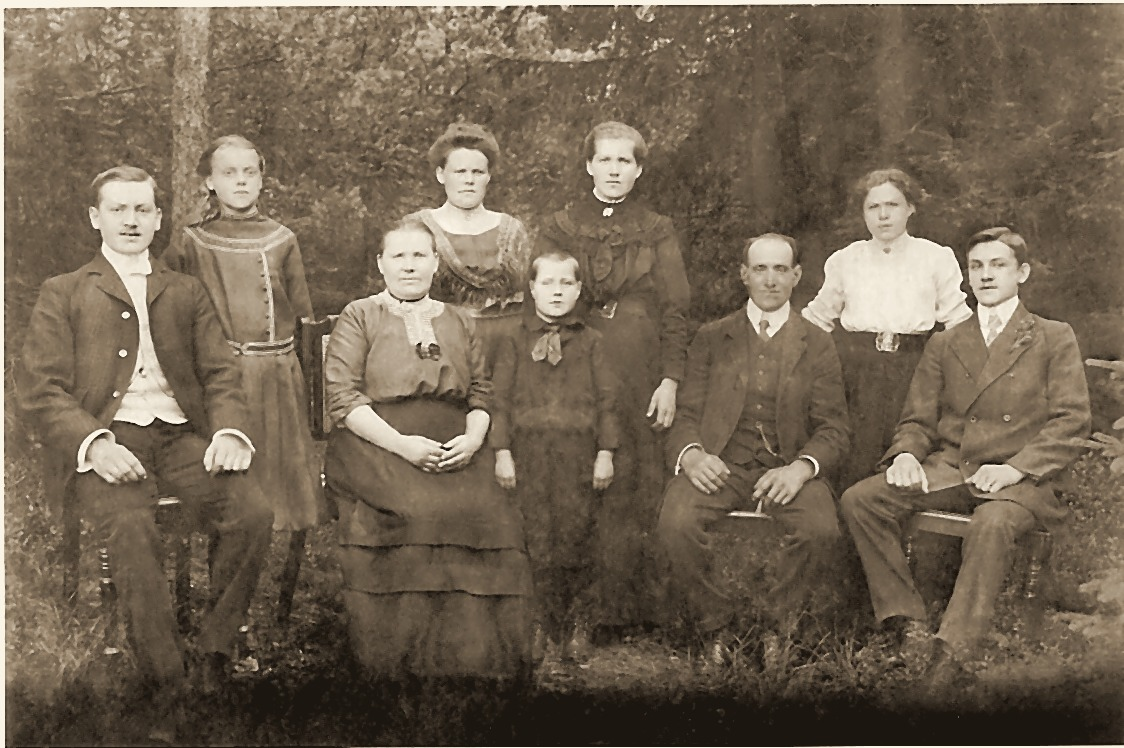
\includegraphics[width=0.85\linewidth,height=\textheight,keepaspectratio,alt={Die Familie der Mota in Deutschland, vor der Abreise 1913. Familienbesitz; wer welche Person ist, muss noch bestätigt werden. Kontrast und Farbtöne korrigiert.}]{imagens/meier_familia_da_mota_alemanha_restaurada.jpg}
\caption{Die Familie der Mota in Deutschland, vor der Abreise 1913.
Familienbesitz; wer welche Person ist, muss noch bestätigt werden.
Kontrast und Farbtöne korrigiert.}
\end{figure}

\section{Der Ziegelknecht, der nicht zu uns
gehörte}\label{der-ziegelknecht-der-nicht-zu-uns-gehuxf6rte}

\emph{Stoffen\index[lugares]{stoffen@Stoffen}, Oberbayern, 1847, und Leonberg\index[lugares]{leonberg@Leonberg}, Oberpfalz\index[lugares]{oberpfalz@Oberpfalz}, 1878}

In den ersten Fassungen dieses Buches begann die andere Seite der
Geschichte in einem Dorf namens Stoffen\index[lugares]{stoffen@Stoffen} bei Landsberg am Lech in
Oberbayern, fast dreihundert Kilometer südwestlich von Heumaden\index[lugares]{heumaden@Heumaden}. Die
Stammbäume im Internet sagten, Josef Haas\index[pessoas]{haas, josef@Haas, Josef}, der Vater des Fata\index[pessoas]{haas, johann@Haas, Johann}, sei dort
am 19. Mai 1847 geboren, Sohn des \emph{Ziegelknechts} Georg Haas und
der Maria Anna Albrecht. Ich fand die Taufe, las das Wort
\emph{Ziegelknecht}, es gefiel mir, und ich schrieb seitenweise über den
Lehm von Stoffen\index[lugares]{stoffen@Stoffen}, den Gips von Sandberg\index[lugares]{sandberg@Sandberg} und das Senklot von Ituporanga\index[lugares]{ituporanga@Ituporanga},
als wären es drei Generationen desselben Handwerks.

Es war ein Namensvetter. Joseph Haas ist ein häufiger Name im
katholischen Bayern\index[lugares]{bayern@Bayern}, und die Taufe von Stoffen\index[lugares]{stoffen@Stoffen} ist echt, aber sie gehört
zu einem anderen Joseph. Aufgeklärt hat den Irrtum das Trauungsbuch von
Leonberg\index[lugares]{leonberg@Leonberg}. Am 4. März 1878 (die standesamtliche Trauung war am 1. März
gewesen) trug der Pfarrer die Heirat von \emph{Haas Joseph} ein, ledig,
\emph{Fabrikarbeiter} in Leonberg\index[lugares]{leonberg@Leonberg}, mit Franziska Dengler\index[pessoas]{dengler, franziska@Dengler, Franziska}, Tochter eines
Bergmanns. In der Spalte für die Eltern des Bräutigams steht klar und
deutlich \emph{Mich. Haas} und \emph{Kunigunde Stadelmann\index[pessoas]{stadelmann, kunigunde@Stadelmann, Kunigunde}}. Nicht Georg
und Maria Anna. Der Großvater des Fata\index[pessoas]{haas, johann@Haas, Johann} hieß Michael.

\begin{ficha}

\textbf{Archivkarte}: Pfarrei Leonberg\index[lugares]{leonberg@Leonberg} (Bistum Regensburg\index[lugares]{regensburg@Regensburg}), Trauungsbuch
1874--1919 (Matricula: \texttt{Leonberg\index[lugares]{leonberg@Leonberg}\_Bul012}), S. 8, Jahrgang 1878,
Eintrag Nr. 4 vom 4. März. Bräutigam: Joseph Haas, ledig,
\emph{Fabrikarbeiter} in Leonberg\index[lugares]{leonberg@Leonberg}; Eltern: \emph{Mich. Haas} und
\emph{Kunigunde Stadelmann\index[pessoas]{stadelmann, kunigunde@Stadelmann, Kunigunde}}. Braut: Franziska Dengler\index[pessoas]{dengler, franziska@Dengler, Franziska} aus Plattenhof,
Tochter der Margaretha Dengler, später verheiratete Rockinger. Die Namen
der Eltern des Bräutigams hat Antigravity gelesen, und ich habe die
Lesung am Bild überprüft. Den Herkunftsort der Eltern, den Antigravity
als Etzgersrieth\index[lugares]{etzgersrieth@Etzgersrieth} liest, habe ich noch nicht überprüft.

\end{ficha}

Und jetzt kommt der Teil, bei dem ich den Stift weglegen musste. Nach
der Lesung von Antigravity, die ich noch mit eigenen Augen überprüfen
muss, stammten Michael Haas\index[pessoas]{haas, michael@Haas, Michael} und Kunigunde Stadelmann\index[pessoas]{stadelmann, kunigunde@Stadelmann, Kunigunde} aus Etzgersrieth\index[lugares]{etzgersrieth@Etzgersrieth},
einem Dorf der Pfarrei Moosbach\index[lugares]{moosbach@Moosbach}, etwa vier Kilometer von Heumaden\index[lugares]{heumaden@Heumaden}
entfernt. Sollte sich das bestätigen, verliert der Satz, den ich weiter
unten in diesem Kapitel geschrieben habe, zwischen den Familien des Fata\index[pessoas]{haas, johann@Haas, Johann}
und der Mota\index[pessoas]{meier, maria@Meier, Maria} hätten fünfzig Kilometer gelegen, seinen Sinn. Die
Großväter der beiden wären in dieselbe Kirche St.~Peter und Paul
gegangen, hätten ihre Kinder am selben Taufbecken taufen lassen und ihre
Toten auf demselben Friedhof begraben. Johann und Maria könnten, bevor
sie ein Brautpaar wurden, Kinder von Nachbarn gewesen sein.

Ich bewahre diese Geschichte vom Ziegelknecht aus Stoffen\index[lugares]{stoffen@Stoffen} hier auf,
statt sie zu löschen, weil sie etwas lehrt, das für eure ganze Forschung
gilt: Ein gleicher Name und ein plausibles Datum ergeben noch keinen
Menschen. Man muss die Eltern prüfen, den Ehepartner, den Ort. Ich habe
das nicht getan und jahrelang einen Mann meinen Ururgroßvater genannt,
der nie zu uns gehörte.

Die Frage, die mir der \emph{Ziegelknecht} gestellt hat, bleibt aber
bestehen, denn sie gilt auch für die echten Haas: Warum haben so viele
aus unserer Familie, auf beiden Seiten des Ozeans, mit ihren Händen an
Dingen gearbeitet, die ihnen nicht gehörten?

Die ehrlichste Antwort, die ich gefunden habe, führt über das Erbe. Im
alten Bayern\index[lugares]{bayern@Bayern} (in Oberbayern, in der Oberpfalz\index[lugares]{oberpfalz@Oberpfalz} von Heumaden\index[lugares]{heumaden@Heumaden}) wurde das
Bauernland nicht unter den Kindern aufgeteilt. Nach Brauch und oft auch
nach Gesetz galt das \emph{Anerbenrecht}. Der Hof ging ungeteilt an
einen Sohn, meist an den ältesten oder an den jüngsten, je nach Gegend.
Die anderen bekamen bestenfalls eine Abfindung in Geld, eine Aussteuer,
das Recht, im Haus zu wohnen, solange sie ledig waren. Dahinter stand
das Überleben des Hofes: Ein Hof, der in jeder Generation zerstückelt
wird, ernährt irgendwann niemanden mehr. Im Rheinland und an der Mosel\index[lugares]{mosel@Mosel},
woher die Vorfahren meiner Mutter kamen, galt das Gegenteil (die
Realteilung, die das Land in immer schmalere Streifen zerschnitt), und
diese andere Geschichte erzähle ich in den Kapiteln von Teil III. Beide
Systeme hatten am Ende dieselbe Wirkung: Sie drängten Menschen vom Land.

In Bayern\index[lugares]{bayern@Bayern} hatte der Bruder, der nicht erbte, wenige Wege. Er konnte als
Knecht auf dem Hof des Bruders bleiben. Er konnte ein Handwerk lernen,
und das waren zu einem guten Teil die Handwerke von Lehm, Stein, Holz
und Eisen. Er konnte in die Stadt gehen, in die Fabriken, die um die
Mitte des Jahrhunderts entstanden. Oder er konnte auswandern. Ich weiß
nicht, ob Michael Haas\index[pessoas]{haas, michael@Haas, Michael} ein Sohn war, der nicht erbte. Ich weiß, dass
sein Sohn Joseph nicht auf dem Land blieb: Er ging in die Fabrik.

Ich will hier nicht alles zur Theorie machen. Auf das Erbe komme ich in
Kapitel 15 zurück, wo es mehr Raum verdient. Ich bitte euch nur, das
Muster zu bemerken, weil es sich wiederholt: das Eisen von Sandberg\index[lugares]{sandberg@Sandberg}, der
Gips des Fata\index[pessoas]{haas, johann@Haas, Johann}, das Senklot von Ituporanga\index[lugares]{ituporanga@Ituporanga}. Generationen von Haas-Männern
haben ihre Familien ernährt, indem sie Dinge bauten, in denen andere
wohnen würden.

\section{Der Rauch der
Maximilianshütte}\label{der-rauch-der-maximilianshuxfctte}

\emph{Sandberg\index[lugares]{sandberg@Sandberg} bei Leonberg\index[lugares]{leonberg@Leonberg}, Oberpfalz\index[lugares]{oberpfalz@Oberpfalz}, Juli 1884}

Irgendwann in seiner Jugend (ich weiß nicht, wann, und nicht, warum)
landete Josef Haas\index[pessoas]{haas, josef@Haas, Josef} in Sandberg\index[lugares]{sandberg@Sandberg} bei Leonberg\index[lugares]{leonberg@Leonberg}, nicht weit von Regensburg\index[lugares]{regensburg@Regensburg}.
Dort gab es seit der Mitte des Jahrhunderts ein Eisenwerk, die
\emph{Maximilianshütte}, benannt nach König Maximilian II. von Bayern\index[lugares]{bayern@Bayern}.
Das Werk gab später der Gemeinde selbst den Namen: Maxhütte-Haidhof\index[lugares]{maxhutte-haidhof@Maxhütte-Haidhof}, zu
der heute Leonberg\index[lugares]{leonberg@Leonberg} und Sandberg\index[lugares]{sandberg@Sandberg} gehören. Es ist der seltene Fall einer
Stadt, die so heißt wie ihre Fabrik.

Ich stelle mir gern vor, was er dort vorfand: die Hochöfen, die das
Eisenerz mit Kohle und eingeblasener Luft schmelzen, in einem Feuer, das
nie ausgeht. Ein Hüttenwerk des 19. Jahrhunderts hatte seinen Geruch,
seinen Lärm und seinen Rauch; an Tagen mit Inversionswetterlage muss der
Himmel tief und grau gehangen haben, der Rauch der Schlote gefangen
unter einem Deckel aus kalter Luft. Ich kenne dieses Phänomen gut: Es
ist dasselbe, das an Wintermorgen im Itajaí\index[lugares]{itajai@Itajaí}-Tal den Nebel unten in den
Tälern festhält, bis die Sonne warm genug ist, um ihn aufzulösen.

In den Dokumenten erscheint Josef als \emph{Fabrikarbeiter}. Er
heiratete Franziska Dengler\index[pessoas]{dengler, franziska@Dengler, Franziska}. Und am 11. Juli 1884, um fünf Uhr
nachmittags, kam in Sandberg\index[lugares]{sandberg@Sandberg} der Sohn zur Welt, den sie Johann nannten:
mein Urgroßvater, der Mann, den die brasilianischen Enkel den Fata\index[pessoas]{haas, johann@Haas, Johann}
nennen würden. Zwei Tage später, am 13. Juli, ging Josef zum Standesamt
Leonberg\index[lugares]{leonberg@Leonberg}, um die Geburt anzuzeigen. Der Eintrag bekam die Nummer 47
jenes Jahres.

Hier gibt es eine kleine Abweichung, die ich festhalten muss, denn
dieses ganze Buch besteht aus ehrlich vermerkten Abweichungen. Vetter
Agenor\index[pessoas]{haas, agenor@Haas, Agenor} schrieb in der Tabelle, die das Rückgrat unserer Genealogie
bildet, Johann sei am „08. Juli 1884`` geboren. Das Standesamtsregister
sagt 11. Juli. Ich halte mich an das Register, angelegt zwei Tage nach
der Geburt nach den Angaben des Vaters selbst. Agenor\index[pessoas]{haas, agenor@Haas, Agenor} arbeitete mit dem,
was er hatte (Familienerinnerung, brasilianische Dokumente, die die
Angaben früherer Dokumente wiederholten), und drei Tage Unterschied nach
einem Jahrhundert und einem Ozean sind fast ein Lob seiner Genauigkeit.

Johann war kein Einzelkind. Agenors Tabelle gibt ihm die Geschwister
Josef, Alois, Georg, Maria, Franziska und Therese. Antigravity hat die
Taufbücher von Leonberg\index[lugares]{leonberg@Leonberg} Seite für Seite gelesen und eine andere Liste
von Kindern des Joseph Haas und der Franziska Dengler\index[pessoas]{dengler, franziska@Dengler, Franziska} gefunden: Barbara
(1879), Joseph (1880), Kunigunda (1882), Johann (1884), Franz Xaver
(1888, mit zwölf Tagen gestorben), Georg (1889) und Sebastian (1891).
Die beiden Listen stimmen nur bei Josef und Georg überein. Ich habe
diese Seiten noch nicht überprüft und lasse deshalb beide Listen hier
nebeneinander stehen. Eine kinderreiche Arbeiterfamilie in einem
Fabrikort. Keines dieser Geschwister taucht in Brasilien auf.

In dieser Lesung steckt eine Einzelheit, die, falls sie sich bestätigt,
eine andere Frage löst. Nach dem Taufbuch von Leonberg\index[lugares]{leonberg@Leonberg} wäre Johann am 8.
Juli 1884 geboren und nicht am 11. Von dort käme dann Agenors Datum.

\begin{figure}
\centering
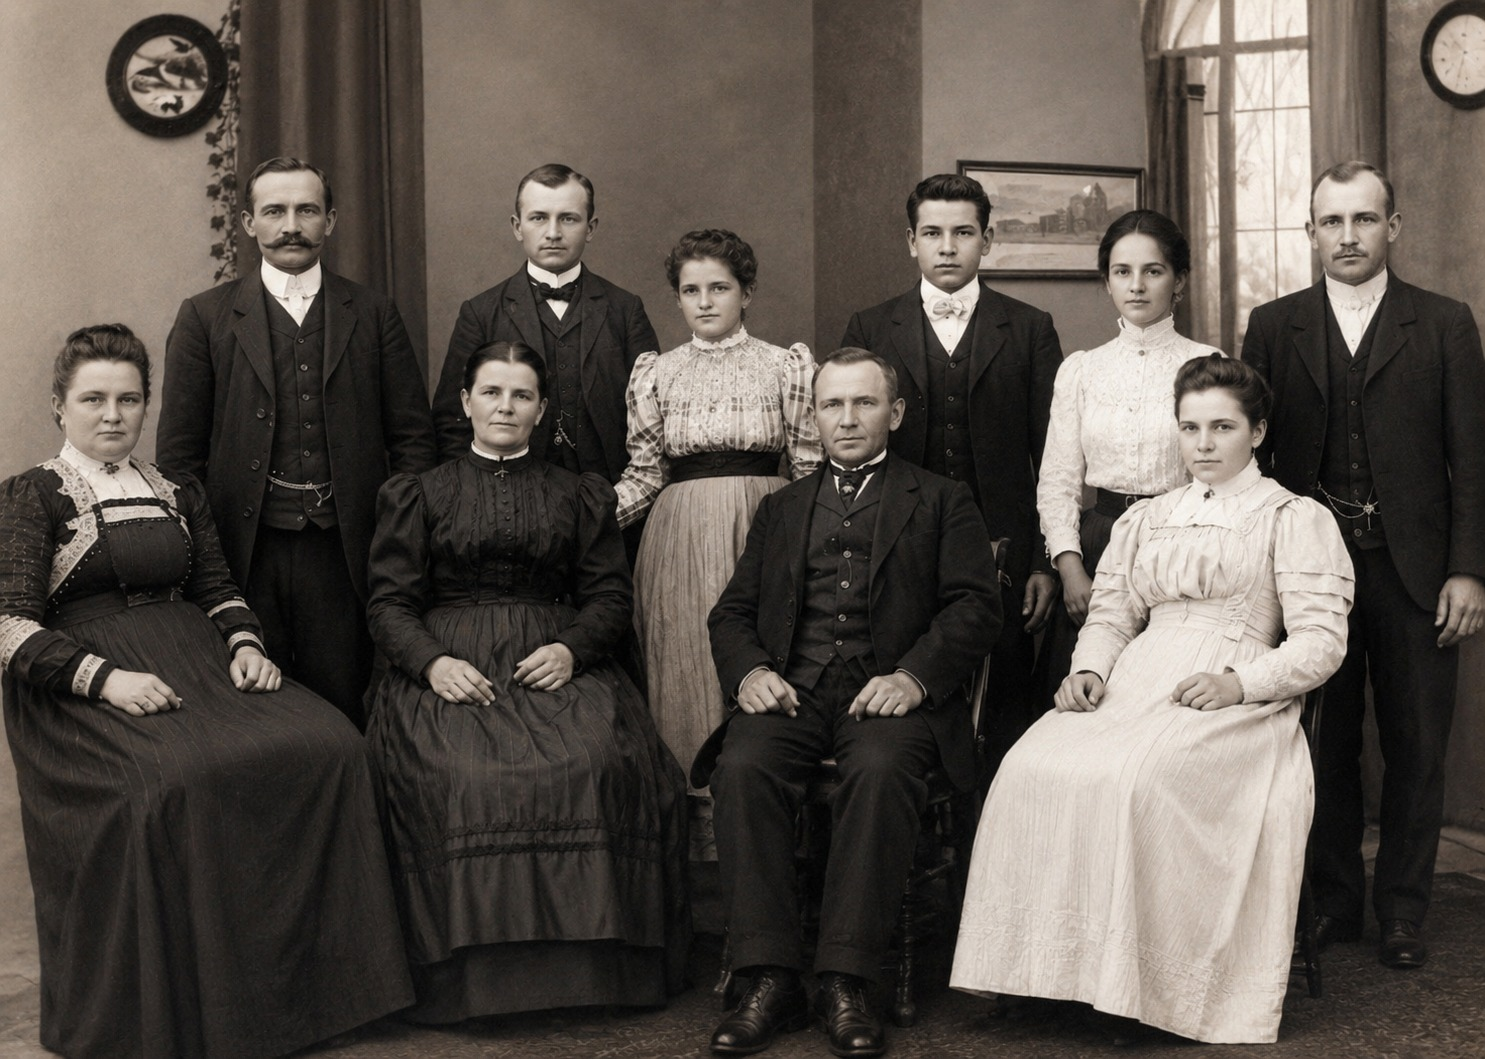
\includegraphics[width=0.85\linewidth,height=\textheight,keepaspectratio,alt={Die Familie des Fata in Deutschland, vor 1913. Familienbesitz; wer welche Person ist, muss im Einzelnen noch bestätigt werden. Mit KI restaurierte Fassung; das Original liegt im Repositorium, und Einzelheiten der Gesichter können retuschiert worden sein.}]{imagens/haas_familia_do_fata_alemanha_restaurada.jpg}
\caption{Die Familie des Fata in Deutschland, vor 1913. Familienbesitz;
wer welche Person ist, muss im Einzelnen noch bestätigt werden. Mit KI
restaurierte Fassung; das Original liegt im Repositorium, und
Einzelheiten der Gesichter können retuschiert worden sein.}
\end{figure}

Dieses Atelierfoto ist mit der allgemeinen Beschriftung „Familie des
Fata\index[pessoas]{haas, johann@Haas, Johann} in Deutschland`` auf uns gekommen. Es zeigt elf Menschen: ein
älteres Paar sitzt in der Mitte, umgeben von jungen Frauen in hellen
Kleidern und jungen Männern mit Weste und Schnurrbart. Es ist verlockend
zu sagen, das sitzende Paar seien Josef und Franziska und einer der
stehenden jungen Männer sei Johann. Ich selbst glaubte, beim Mann mit
Schnurrbart links eine gewisse Geometrie des Gesichts wiederzuerkennen.
Aber ich weiß es nicht. Soweit ich weiß, stehen auf der Rückseite keine
Namen. Ich lasse die Frage lieber offen, wie eine Station ohne Daten,
als die Karte mit einer Vermutung zu füllen, die später jemand als
Gewissheit zitiert.

Was die Familie über Johann bewahrt hat, betrifft sein Handwerk. Der
Text zum hundertjährigen Jubiläum, den meine Schwester Marise\index[pessoas]{lourenco, marise haas@Lourenço, Marise Haas} Haas
Lourenço 2013 schrieb, sagt, er „stammte aus einer Maurerfamilie und
hatte sich auf die Arbeit mit Gips spezialisiert, er fasste Fenster,
Portale und Altäre ein``. Ein Stuckateur also: der Handwerker, der
kommt, nachdem der Maurer die Wand hochgezogen hat, um ihr Form und
Schmuck zu geben. Die Gesimse der bayerischen Barockkirchen, die
Medaillons an den Decken, die Fensterumrahmungen der Bürgerhäuser: All
das war Arbeit von Stuckateuren. Es war ein Handwerk für feine Hände und
viel Geduld: den Gips in der richtigen Konsistenz anrühren, die
Profilschablone an der Wand entlangziehen, Blätter, Engel und Voluten
von Hand modellieren.

Johann kam aus einer Fabrikstadt, Sohn eines Arbeiters. Dass er bis zum
Zierstuck gelangte, ist für mich ein kleiner sozialer Aufstieg: vom Arm,
der den Ofen füttert, zur Hand, die zeichnet. Marise\index[pessoas]{lourenco, marise haas@Lourenço, Marise Haas} hat noch eine
Einzelheit festgehalten, die mich bewegt: Man rief ihn oft als
Dolmetscher, weil er mehrere deutsche Dialekte beherrschte, „die in
einem Land, dessen Sprache noch nicht vereinheitlicht war, noch sehr
lebendig waren``. Das Deutschland von 1900 war ein junges Land,
politisch erst seit drei Jahrzehnten geeint, und ein Bayer aus der
Oberpfalz\index[lugares]{oberpfalz@Oberpfalz} konnte echte Mühe haben, einen Sachsen\index[lugares]{sachsen@Sachsen}, einen Schwaben oder
einen Norddeutschen zu verstehen. Ich stelle mir Johann auf den
Baustellen vor, zwischen Arbeitertrupps von überallher, wie er die
Anweisungen des Poliers in den Dialekt eines jeden übersetzt. Ein Mann
mit gutem Gehör, der den Tonfall wechselte, wie man ein Werkzeug
wechselt.

Vielleicht war er deshalb später der Geschichtenerzähler, an den sich
die Enkel erinnern. Wer sein Leben lang übersetzt, lernt, dass jeder
Satz mindestens zwei Fassungen hat.

\begin{figure}
\centering
\includegraphics[width=0.9\linewidth,height=\textheight,keepaspectratio,alt={Woher sie kamen: die Herkunftsorte der Familienzweige in Europa. Die Punkte mit Fragezeichen stammen aus der Überlieferung, nicht aus Dokumenten. Karte des Autors.}]{imagens/mapa_europa_origens.jpg}
\caption{Woher sie kamen: die Herkunftsorte der Familienzweige in
Europa. Die Punkte mit Fragezeichen stammen aus der Überlieferung, nicht
aus Dokumenten. Karte des Autors.}
\end{figure}

\section{Eibenstock, August 1907}\label{eibenstock-august-1907}

Ich weiß nicht, wie Johann und Maria sich kennengelernt haben.

Das ist der Satz, der mir in diesem Kapitel am schwersten fällt. Er aus
einem Hüttenort bei Regensburg\index[lugares]{regensburg@Regensburg}, sie aus einem Bauerndorf an der
böhmischen Grenze. Zwischen Sandberg\index[lugares]{sandberg@Sandberg} und Heumaden\index[lugares]{heumaden@Heumaden} liegen etwa fünfzig
Kilometer Luftlinie, weit genug, dass sich zwei junge Leute aus diesen
Familien kaum zufällig auf einem Kirchenfest begegnet wären. Und doch
sind sie sich begegnet. Wenn Johanns Großeltern tatsächlich aus
Etzgersrieth\index[lugares]{etzgersrieth@Etzgersrieth} kamen, wie ich oben erzählt habe, schrumpft die Entfernung
auf vier Kilometer, und den Zufall braucht es nicht mehr.

Vetter Agenor\index[pessoas]{haas, agenor@Haas, Agenor} notierte, dass sie am 3. August 1907 in Eibenstock\index[lugares]{eibenstock@Eibenstock}
geheiratet haben. Wenn es das Eibenstock\index[lugares]{eibenstock@Eibenstock} ist, das ich von den Landkarten
kenne, liegt es nicht in Bayern\index[lugares]{bayern@Bayern}, sondern in Sachsen\index[lugares]{sachsen@Sachsen}, im Erzgebirge, nahe
der böhmischen Grenze: eine Gegend des Bergbaus, der Stickerei und der
Talsperren, etwa hundert Kilometer von Heumaden\index[lugares]{heumaden@Heumaden} und deutlich weiter von
Sandberg\index[lugares]{sandberg@Sandberg} entfernt. Den Eintrag dieser Hochzeit habe ich noch nicht
gesehen; ich weiß nicht, in welcher Kirche sie stattfand und wer die
Trauzeugen waren. Sachsen\index[lugares]{sachsen@Sachsen} war überwiegend lutherisch, und die beiden
waren katholisch. All das macht Eibenstock\index[lugares]{eibenstock@Eibenstock} zu einer der offenen Fragen
dieses Buches.

Ich habe eine Hypothese, und ich stelle sie als Hypothese vor. Johanns
Arbeit war ihrer Natur nach Wanderarbeit: Der Stuckateur geht dorthin,
wo gebaut wird. Und auch Marias Arbeit führte sie laut Marise\index[pessoas]{lourenco, marise haas@Lourenço, Marise Haas} aus dem
Haus: „Maria verdiente, neben der Hausarbeit, Lohn mit dem Melken von
Kühen.`` Ein neunzehnjähriges Mädchen, Tochter eines kleinen Bauern mit
sieben Kindern, das gegen Lohn Kühe molk, also auf fremden Höfen. Das
ist das Bild einer Tochter, die nicht erben würde. Wieder das
\emph{Anerbenrecht}: Das Land der Meiers in Heumaden\index[lugares]{heumaden@Heumaden} würde an einen
einzigen der Brüder gehen, und die anderen mussten ihr Auskommen suchen,
wo es Arbeit gab. Es ist durchaus möglich, dass die beiden sich fern von
zu Hause begegnet sind, beide im Dienst anderer, an einem Ort, der
keinem von ihnen gehörte. Aber mehr ist es nicht: eine Möglichkeit.

Zwei Spuren geben dieser Möglichkeit eine Adresse. Die erste ist eine
Familienerinnerung: Als sie 1913 nach Brasilien aufbrachen, wohnten
Johann und Maria in Chemnitz\index[lugares]{chemnitz@Chemnitz}, der großen Industriestadt Sachsens, der
Stadt der Textil- und Maschinenfabriken, die in jenen Jahren schnell
wuchs und Maurer brauchte. Die zweite liegt in einer Schublade der
Familie: Briefe aus Deutschland mit der Absenderadresse Dorfstadt\index[lugares]{dorfstadt@Dorfstadt}, einem
Ortsteil von Falkenstein\index[lugares]{falkenstein@Falkenstein} im Vogtland\index[lugares]{vogtland@Vogtland}. Eibenstock\index[lugares]{eibenstock@Eibenstock} liegt zwischen beiden,
am Rand des Erzgebirges, ein paar Dutzend Kilometer von Falkenstein\index[lugares]{falkenstein@Falkenstein} und
etwas weiter von Chemnitz\index[lugares]{chemnitz@Chemnitz} entfernt. Wenn die Erinnerung stimmt, ist die
Hochzeit von 1907 kein geographisches Rätsel mehr: Es war keine Reise
nach Sachsen\index[lugares]{sachsen@Sachsen}, sondern eine Hochzeit in der Gegend, in der die beiden
schon lebten und arbeiteten. Und ein wahrscheinliches Warum tauchte 2026
auf, in den Briefen, von denen ich in Kapitel 7 erzähle: Marias Familie
verließ Heumaden\index[lugares]{heumaden@Heumaden} und landete im Vogtland\index[lugares]{vogtland@Vogtland}, bei Falkenstein\index[lugares]{falkenstein@Falkenstein}, wo 1971 noch
drei Schwestern und ein Bruder von ihr lebten. Wenn sie 1907 schon dort
waren, hat Maria in der Nähe ihrer Mutter geheiratet. Und noch immer
fehlt das Papier. Es steht im Trauungsbuch von Eibenstock\index[lugares]{eibenstock@Eibenstock} und, falls die
Kinder dort geboren wurden, in den Registern von Chemnitz\index[lugares]{chemnitz@Chemnitz}.

Was Marise\index[pessoas]{lourenco, marise haas@Lourenço, Marise Haas} sagt und was die Familie immer wiederholt hat: Sie heirateten
jung, „mit dem Traum, der uns allen so eigen ist, eine Familie zu
gründen``. Johann war dreiundzwanzig, Maria neunzehn. Marise\index[pessoas]{lourenco, marise haas@Lourenço, Marise Haas} fügt einen
Satz hinzu, den ich treffend finde: Sie war es, „die sich mit der Arbeit
auf dem Land auskannte, und gewiss der Halt für die große Reise, die sie
bald antreten sollten``.

\begin{figure}
\centering
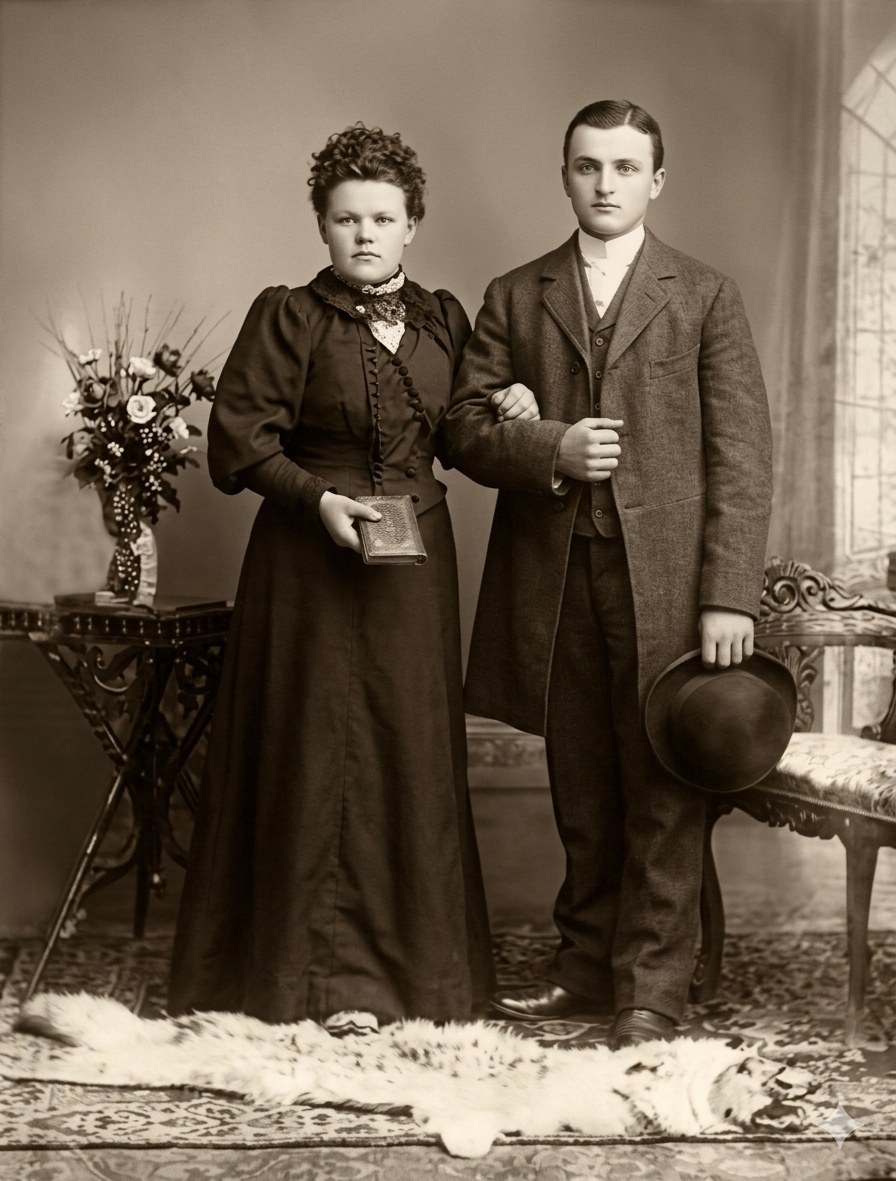
\includegraphics[width=0.6\linewidth,height=\textheight,keepaspectratio,alt={Johann und Maria, der Fata und die Mota, auf dem Hochzeitsbild, wahrscheinlich vom August 1907. Familienbesitz. Mit künstlicher Intelligenz überarbeitete Fassung einer alten Kopie: Hintergrund und Schärfe der Gesichter könnten von der Maschine retuschiert sein; Haltung, Kleidung und Personen sind die des Originals.}]{imagens/haas_casamento_fata_e_mota_1907_versao_ia.jpg}
\caption{Johann und Maria, der Fata und die Mota, auf dem Hochzeitsbild,
wahrscheinlich vom August 1907. Familienbesitz. Mit künstlicher
Intelligenz überarbeitete Fassung einer alten Kopie: Hintergrund und
Schärfe der Gesichter könnten von der Maschine retuschiert sein;
Haltung, Kleidung und Personen sind die des Originals.}
\end{figure}

Das ist ihr Hochzeitsbild. Es entstand im Atelier eines Fotografen, vor
einem gemalten Hintergrund, mit einem Blumentischchen auf der einen und
einem Polsterstuhl auf der anderen Seite, wie man es damals in ganz
Deutschland machte. Maria trägt ein dunkles Kleid mit Puffärmeln und
Spitzenkragen und hält ein Büchlein in der Hand, wohl das Messbuch oder
Gebetbuch. Das weiße Brautkleid war noch ein Luxus reicher Leute; die
Bräute aus dem Volk heirateten in Schwarz, im besten Kleid, das sie
hatten, und trugen es danach ein Leben lang an Sonntagen. Johann trägt
Überzieher, Weste und hohen Kragen, den Hut in der Hand. Sie stützt sich
auf seinen Arm. Beide blicken ernst in die Kamera, mit den runden
Gesichtern von neunzehn und dreiundzwanzig Jahren. Keiner von beiden
ahnte an diesem Tag, dass sie sechs Jahre später auf einem Schiff nach
Brasilien sitzen würden und dass dieses Bild mit ihnen über den Ozean
reisen und bis in eure Hände gelangen würde.

\begin{figure}
\centering
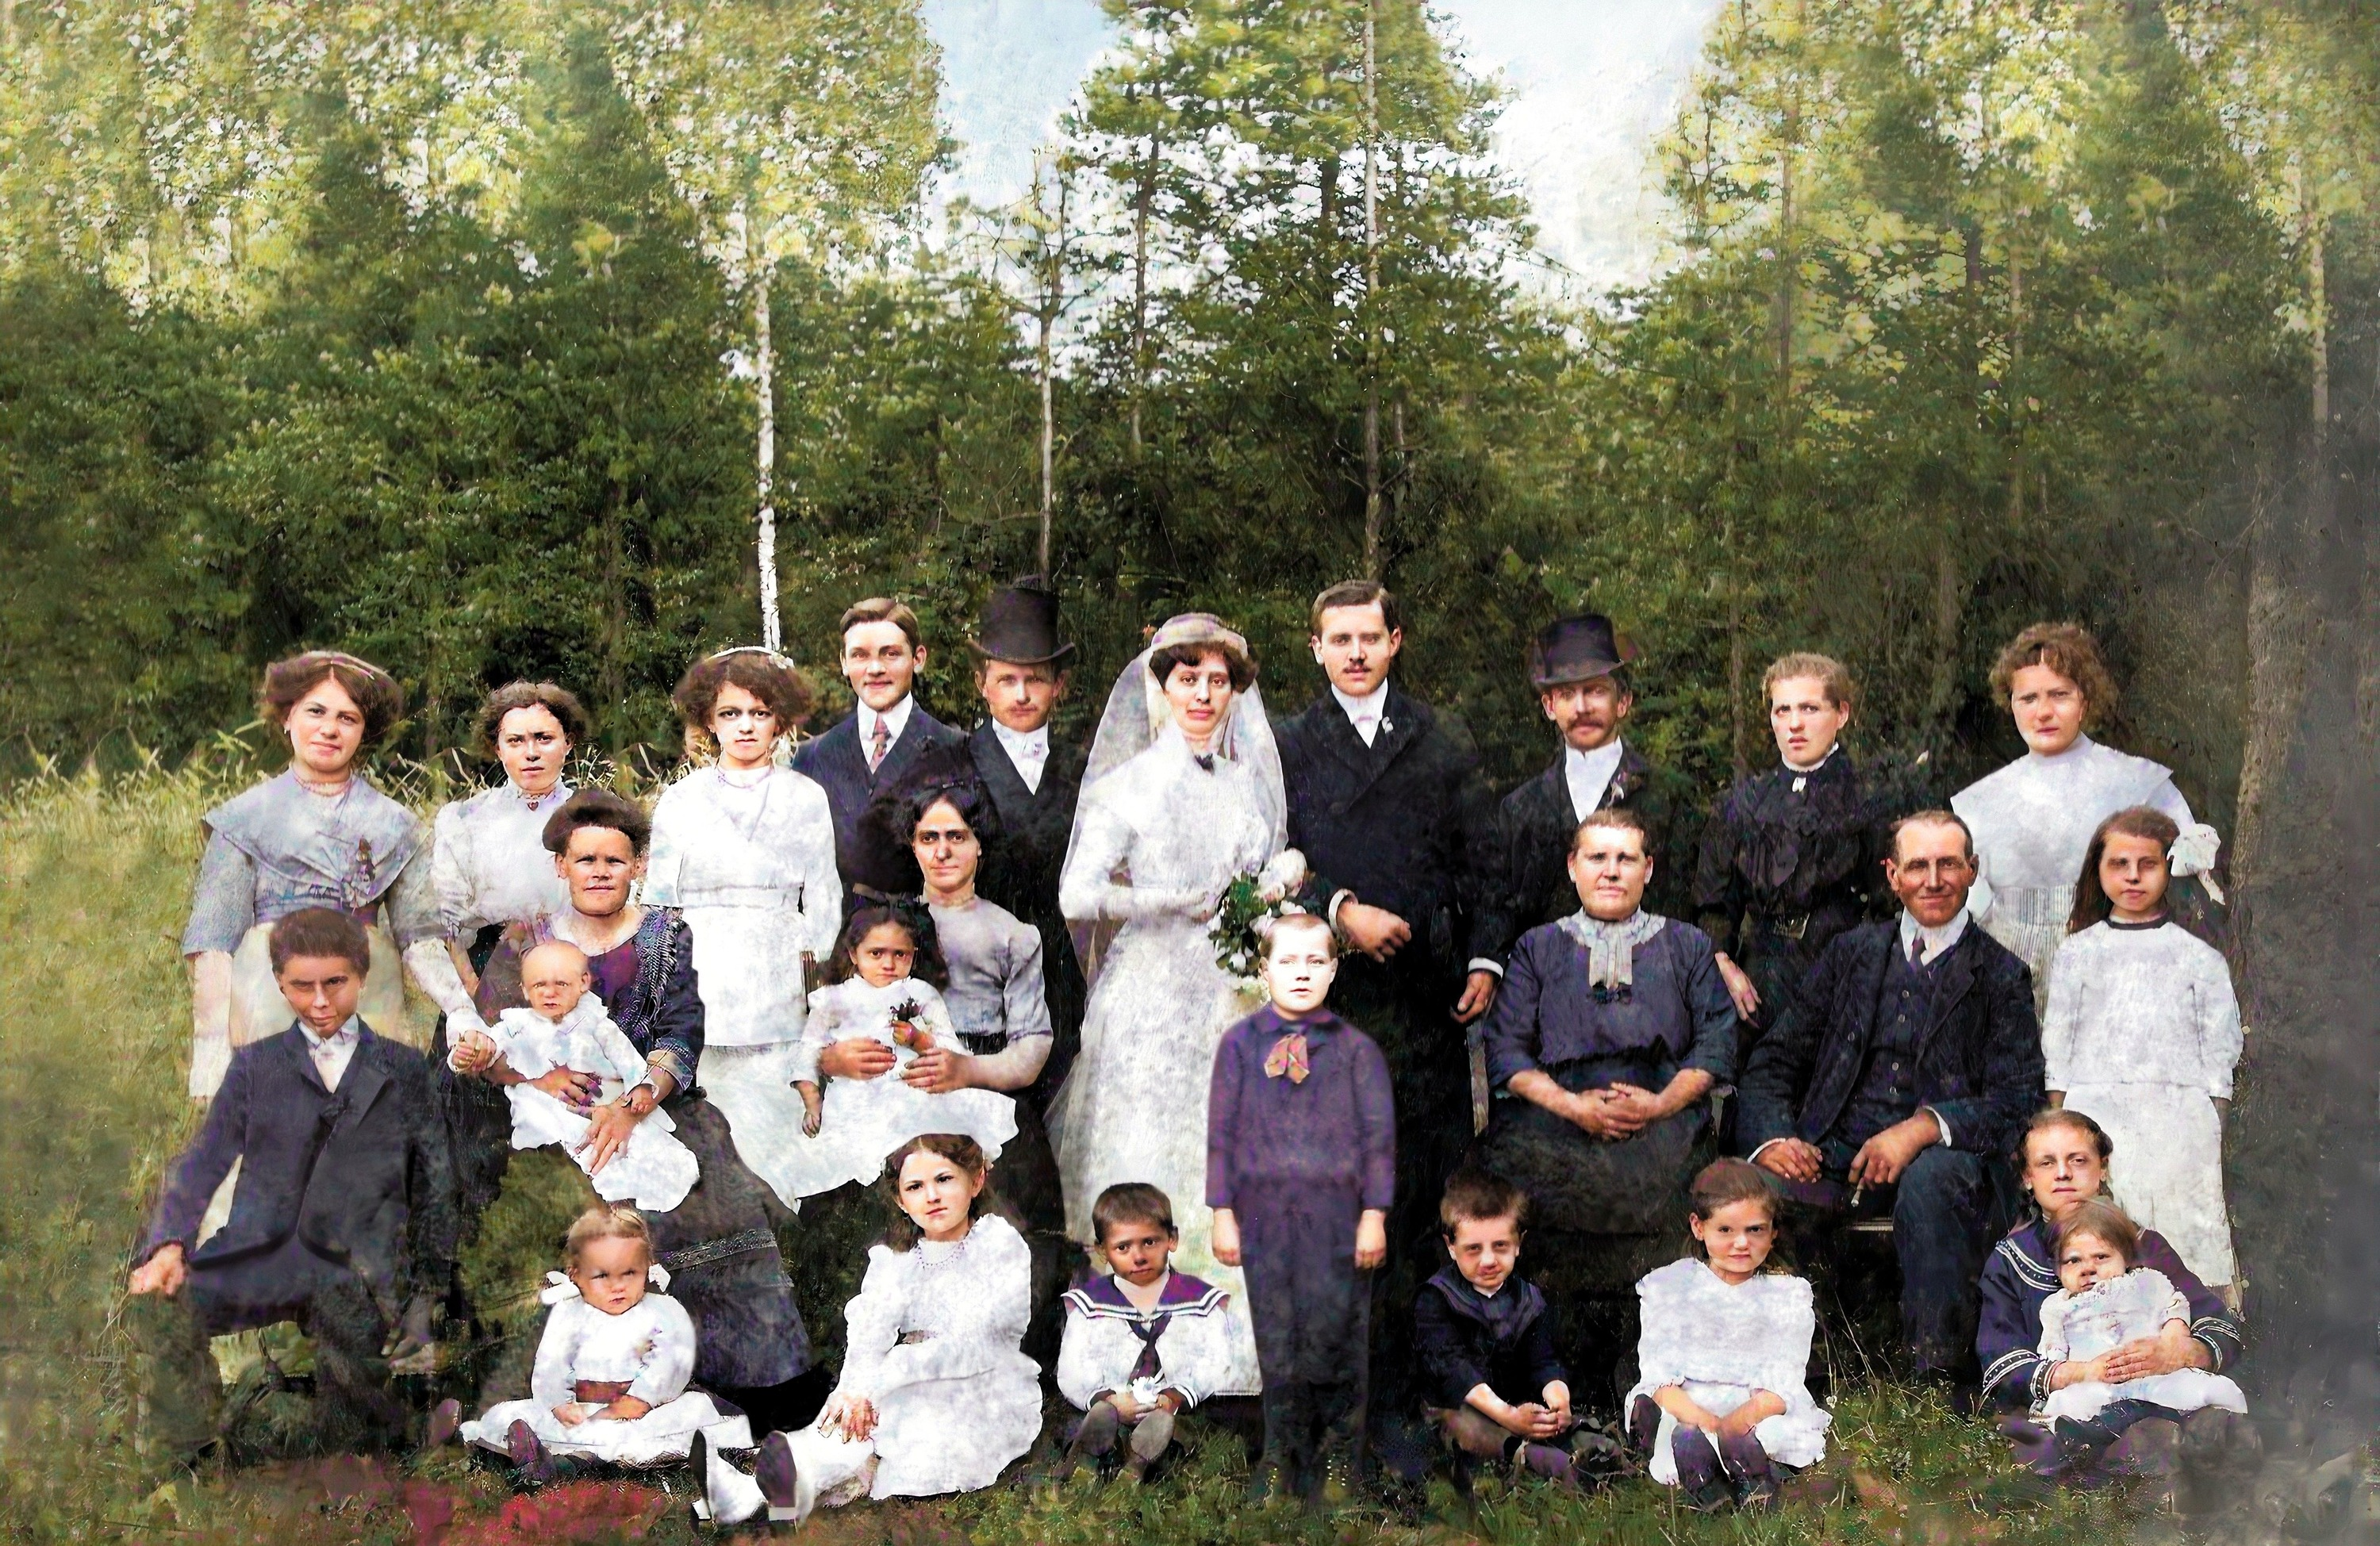
\includegraphics[width=0.85\linewidth,height=\textheight,keepaspectratio,alt={Hochzeitsfoto aus der Familie der Mota in Deutschland, auf einer Waldlichtung. Familienbesitz. Links sitzend, mit einem Baby auf dem Schoß, die Mota; das Brautpaar ist noch nicht identifiziert. Mit KI kolorierte und restaurierte Fassung (MyHeritage); die Farben sind eine Rekonstruktion, und das Schwarzweiß-Original liegt im Repositorium.}]{imagens/meier_familia_da_mota_alemanha_casamento_restaurada.jpg}
\caption{Hochzeitsfoto aus der Familie der Mota in Deutschland, auf
einer Waldlichtung. Familienbesitz. Links sitzend, mit einem Baby auf
dem Schoß, die Mota\index[pessoas]{meier, maria@Meier, Maria}; das Brautpaar ist noch nicht identifiziert. Mit KI
kolorierte und restaurierte Fassung (MyHeritage); die Farben sind eine
Rekonstruktion, und das Schwarzweiß-Original liegt im Repositorium.}
\end{figure}

Dieses andere Foto hat mich immer beschäftigt. Es ist eine Hochzeit, im
Freien aufgenommen, auf einer Lichtung zwischen Tannen und Birken: die
Braut mit Schleier und Strauß, der Bräutigam mit schmalem Schnurrbart,
zwei Männer mit Zylinder, ein Dutzend Kinder im Sonntagsstaat, die im
Gras sitzen, ältere Frauen in Schwarz und junge Frauen in Weiß. Es kam
zu mir als „Hochzeit in der Familie der Mota\index[pessoas]{meier, maria@Meier, Maria}``, und jahrelang habe ich
mich gefragt, ob es die Hochzeit von Johann und Maria ist. Sie ist es
nicht. Die Familie hat die Mota\index[pessoas]{meier, maria@Meier, Maria} erkannt: Sie sitzt links, im dunklen
Kleid, mit einem Baby auf dem Schoß. Sie war also schon Mutter, und das
Foto ist nach 1908 entstanden. Das Baby kann Hildegard, Frida, Luisa\index[pessoas]{haas, luisa@Haas, Luisa}
oder Walter sein; die Blätter an den Birken sagen, dass es Sommer war.

Wessen Hochzeit war es? Ich habe die Gesichter dieses Fotos neben die
des Abschiedsfotos von 1913 und die der Familie der Mota\index[pessoas]{meier, maria@Meier, Maria} im Wäldchen
gestellt.

\begin{figure}
\centering
\includegraphics[width=0.95\linewidth,height=\textheight,keepaspectratio,alt={In der ersten Reihe das Abschiedsfoto von 1913: die Frau links, der Mann mit Schnurrbart, die Mota und der Fata. In der zweiten das Hochzeitsfoto: die ältere Frau und der ältere Mann, die rechts sitzen, die Mota mit dem Baby, die Braut, der Bräutigam, der Mann mit Zylinder und Schnurrbart rechts vom Bräutigam und die junge Frau, die neben der Mota sitzt. In der dritten das Familienfoto im Wäldchen: die ältere Frau und der ältere Mann, der Mann mit Schnurrbart links, der junge Mann rechts und drei junge Frauen, die hinten stehen.}]{imagens/rostos_tres_fotos_meier.jpg}
\caption{In der ersten Reihe das Abschiedsfoto von 1913: die Frau links,
der Mann mit Schnurrbart, die Mota\index[pessoas]{meier, maria@Meier, Maria} und der Fata\index[pessoas]{haas, johann@Haas, Johann}. In der zweiten das
Hochzeitsfoto: die ältere Frau und der ältere Mann, die rechts sitzen,
die Mota\index[pessoas]{meier, maria@Meier, Maria} mit dem Baby, die Braut, der Bräutigam, der Mann mit Zylinder
und Schnurrbart rechts vom Bräutigam und die junge Frau, die neben der
Mota\index[pessoas]{meier, maria@Meier, Maria} sitzt. In der dritten das Familienfoto im Wäldchen: die ältere Frau
und der ältere Mann, der Mann mit Schnurrbart links, der junge Mann
rechts und drei junge Frauen, die hinten stehen.}
\end{figure}

Ich sehe drei Übereinstimmungen, und mehr als Übereinstimmungen sind es
nicht. Das ältere Paar, das auf der Hochzeit rechts sitzt, hat dieselben
Gesichter wie das sitzende Paar im Wäldchen: die Frau mit dem runden
Gesicht und dem Spitzenkragen, der Mann mit der hohen Stirn und den
großen Ohren. Wenn es dasselbe Paar ist, ist es die Familie Meier, und
die beiden wären Georg Adam und Franziska, die Eltern der Mota\index[pessoas]{meier, maria@Meier, Maria}. Dann ist
es die Hochzeit eines ihrer Kinder. Der Bräutigam wiederum erinnert
stark an den Mann mit Schnurrbart, der auf dem Foto im Wäldchen links
sitzt. Und die dunkelhaarige Braut passt gut zu der Frau links auf dem
Abschiedsfoto von 1913.

Wenn sich das alles bestätigt, schließt sich die Geschichte auf eine
Weise, die ich nicht zu erfinden wagte: Dies ist die Hochzeit einer
Schwester der Mota\index[pessoas]{meier, maria@Meier, Maria}, vielleicht mit Walter Heckel\index[pessoas]{heckel, walter@Heckel, Walter}, und dieses Paar stand
im März 1913 mit seinem kleinen Kind neben Johann und Maria, für das
Foto, das bei ihnen bleiben sollte. Und diese Schwester schrieb
achtundfünfzig Jahre später aus Rempesgrün\index[lugares]{rempesgrun@Rempesgrün}, sie habe den Abschied am
Bahnhof nie vergessen. Das sind viele „Wenn``. Die Namen von Braut und
Bräutigam müssen im Heiratsregister eines Standesamts im Vogtland\index[lugares]{vogtland@Vogtland}
stehen, um 1908 bis 1912, und den Schlüssel zu dieser Tür haben die
Verwandten dort.

Wo wurde das Foto aufgenommen? Ich entscheide mich für das Vogtland\index[lugares]{vogtland@Vogtland},
wahrscheinlich für Rempesgrün\index[lugares]{rempesgrun@Rempesgrün} oder die Umgebung. Den Ausschlag gibt die
Familie: Die Meiers verschwinden nach 1892 aus den Moosbacher Büchern,
und 1971 lebten die Schwestern der Mota\index[pessoas]{meier, maria@Meier, Maria} noch dort, zwischen Rempesgrün\index[lugares]{rempesgrun@Rempesgrün}
und Dorfstadt\index[lugares]{dorfstadt@Dorfstadt}. Eine Hochzeit ihrer Kinder um 1910 fand wohl dort statt.
Die Landschaft bestätigt, was die Familie nahelegt. Das Vogtland\index[lugares]{vogtland@Vogtland} liegt
höher und ist kälter als die Gegend um Heumaden\index[lugares]{heumaden@Heumaden}, ein Land der Fichten
und Birken, und genau dieser dunkle, dichte Wald steht im Hintergrund
aller drei Fotos: der Hochzeit, der Familie im Wäldchen und des
Abschieds von 1913. Ich halte diese Entscheidung als meine fest, damit
ihr wisst, dass sie eine Deutung ist und kein Dokument. Wenn eines Tages
der Heiratseintrag auftaucht oder der Stempel eines Fotografen auf der
Rückseite einer Kopie, dann gilt der.

Die ersten Ehejahre, schrieb Marise\index[pessoas]{lourenco, marise haas@Lourenço, Marise Haas}, „erwiesen sich als schwer und
leidvoll``. Hier kommen wir zu dem Teil des Kapitels, den ich am
liebsten überspringen würde.

Johann und Maria bekamen in Deutschland zwei Töchter, die klein starben:
Hildegard (Agenor\index[pessoas]{haas, agenor@Haas, Agenor} schreibt Hildegart) und Frida. Wir kennen weder die
Geburtsdaten noch die Sterbedaten noch die Ursache. „Aus Gründen, die
wir nicht kennen``, sagt der Jubiläumstext, mit einer Nüchternheit, die
ich respektiere. Wir wissen nicht, wo sie begraben sind. Vielleicht in
Eibenstock\index[lugares]{eibenstock@Eibenstock}, vielleicht an einem anderen Ort, an den die Arbeit das Paar
geführt hatte.

1907 war die Säuglingssterblichkeit in Deutschland noch hoch; in vielen
ländlichen Gegenden und Arbeitervierteln erlebte eines von fünf Kindern
seinen ersten Geburtstag nicht. Das zu sagen, mindert nichts. Ich habe
selbst zwei Söhne und kann „Hildegard und Frida`` nicht lesen, ohne kurz
innezuhalten. Es sind die ersten beiden Namen einer Liste, die dieses
Buch bis zum Ende tragen wird, der Liste der Kinder, die es nicht
geschafft haben: fünf der zwölf Kinder des Fata\index[pessoas]{haas, johann@Haas, Johann} und der Mota\index[pessoas]{meier, maria@Meier, Maria}. Die
anderen drei Namen nenne ich noch nicht. Ihr, Matheus und Lucas, seid
da, weil die anderen sieben durchgehalten haben.

\section{Luisa, Walter und die
Entscheidung}\label{luisa-walter-und-die-entscheidung}

\emph{Deutschland, 1910 bis 1913}

1910 wurde Luisa\index[pessoas]{haas, luisa@Haas, Luisa} geboren, 1912 Walter. Zwei lebende Kinder nach zwei
Verlusten. Ich weiß nicht, wo sie geboren wurden; die Register, nach
denen ich suche, sind noch nicht aufgetaucht. Ich weiß, dass sie im März
1913 lebten und gesund genug waren, um mit dem Zug quer durch Europa zu
fahren und in Marseille\index[lugares]{marseille@Marseille} an Bord eines Schiffes zu gehen, und das weiß
ich aus einem Dokument, das ich im nächsten Kapitel zeige und in dem die
beiden mit zwei Jahren und einem Jahr verzeichnet sind.

Ende 1912 wurde Maria wieder schwanger. Jedenfalls ergibt sich das aus
Marises Text, denn Vetter Agenor\index[pessoas]{haas, agenor@Haas, Agenor} hat die Dinge anders festgehalten.

In seiner Tabelle steht eine Tochter namens Gertrudes, geboren in
Deutschland am 22. Oktober 1911, die mit einem Jahr auf dem Schiff
mitgekommen wäre. Marises Text sagt etwas anderes: dass Gertrudes im Mai
1913 in Brasilien geboren wurde und Maria mit ihr schwanger an Bord
ging. Beide Fassungen können nicht zugleich stimmen, und im nächsten
Kapitel stelle ich sie nebeneinander, zusammen mit dem Dokument, das
schwerer wiegt. Vorerst folge ich Marise\index[pessoas]{lourenco, marise haas@Lourenço, Marise Haas}: Im März 1913 hatten Johann und
Maria zwei kleine Kinder und ein drittes unterwegs.

Was bringt ein solches Paar dazu fortzugehen?

Marise\index[pessoas]{lourenco, marise haas@Lourenço, Marise Haas} spricht von der „großen wirtschaftlichen und politischen Krise``
in Deutschland und von dem „drohenden Krieg``, der „das Paar
verfolgte``. Mir gefällt, dass sie nicht vereinfacht hat. Das
Deutschland von 1912 war zugleich eine Industriemacht in voller
Expansion und ein Land enormer Ungleichheit, in dem die
Lebenshaltungskosten schneller stiegen als die Löhne der Arbeiter und
Landarbeiter. Und die Luft war geladen. Die Balkankrisen, das
Flottenwettrüsten mit England, die von Jahr zu Jahr wachsenden
Militärhaushalte: All das erreichte die Dörfer über die Zeitungen und
die Gespräche im Wirtshaus. Niemand wusste genau, was geschehen würde,
aber viele ahnten, dass etwas geschehen würde. In der Meteorologie
nennen wir das Labilität: Die Atmosphäre sammelt Energie, die Luftsäule
ist bereit aufzusteigen, und es fehlt nur noch ein Auslöser.

Für einen jungen Familienvater bedeutete Krieg etwas sehr Konkretes: die
Einberufung. Johann war achtundzwanzig. Es ist möglich (und hier
spekuliere ich wieder), dass die Angst, eingezogen zu werden und Maria
mit den Kindern allein zu lassen, ebenso schwer wog wie das fehlende
Geld.

Auf der anderen Seite des Ozeans lag Brasilien. Seit dem Ende des 19.
Jahrhunderts warben die brasilianische Regierung und die Regierungen der
Südstaaten in Europa um Siedler: billiges Land, in Raten zahlbar,
Werkzeug, Saatgut, Hilfe in den ersten Monaten. In Santa Catarina hatte
die Bundesregierung kurz zuvor im Landesinneren, an den Hängen des
Gebirges, eine Siedlungskolonie gegründet und sie Anitápolis\index[lugares]{anitapolis@Anitápolis} genannt, zu
Ehren von Anita Garibaldi, der Heldin von Laguna\index[lugares]{laguna@Laguna}. Dorthin sollten die
Haas gehen, auch wenn das an dem Tag, an dem sie den Aufbruch
beschlossen, noch nicht feststand. Marise\index[pessoas]{lourenco, marise haas@Lourenço, Marise Haas} schreibt, sie gingen „ins
Paradies``, in Anführungszeichen, die von ihr stammen und die ganze
Ironie dessen tragen, der weiß, was danach kam.

Ich vermute, dass das Land selbst das entscheidende Argument war. Ein
Maurer, Sohn eines Arbeiters, und eine Melkerin, Tochter eines kleinen
Bauern mit sieben Kindern: Keiner der beiden würde in Bayern\index[lugares]{bayern@Bayern} je ein
Stück Boden erben. Nicht, wenn sie hundert Jahre alt würden. Das
\emph{Anerbenrecht} hatte diese Tür verschlossen, noch bevor sie geboren
waren. In Brasilien, so stand es in den Prospekten, warteten
Siedlerparzellen, die \emph{lotes coloniais}, auf jeden, der arbeiten
wollte.

Marise\index[pessoas]{lourenco, marise haas@Lourenço, Marise Haas} besteht auf einem Punkt, den ich wichtig finde und nicht
weglassen will: Die Entscheidung „war weder willkürlich noch
einseitig``. Beide kamen aus gefestigten Familien, in denen „das Gewicht
der Meinung der Eltern ebenso groß war wie der Respekt, den die Kinder
ihnen entgegenbrachten``. Es gab Gespräche, Stimmen dafür und dagegen.
Ich stelle mir den Küchentisch in Heumaden\index[lugares]{heumaden@Heumaden} vor, an einem Winterabend,
Georg Adam und Franziska, die hören, wie die Tochter sagt, sie gehe mit
dem Mann und den Enkeln fort, in ein Land, von dem sie kaum den Namen
der Hauptstadt kannten. Ich stelle mir die Stille danach vor.

\emph{Und wenn ihr nicht zurückkommt?}

Ich weiß nicht, ob jemand diesen Satz gesagt hat. Aber jemand muss ihn
gedacht haben, denn das Foto, das sie vor der Abreise machen ließen,
sieht aus wie ein endgültiger Abschied. Marise\index[pessoas]{lourenco, marise haas@Lourenço, Marise Haas} schrieb, sie hätten sich
verabschiedet „mit Gesten, aus denen die Gewissheit sprach, dass sie
sich nie wiedersehen würden``. Sie hatte recht: Sie haben sich nie
wiedergesehen.

Ich möchte dieses Kapitel mit einer Übung beenden, die ich bei der
Arbeit oft mache. Wenn ich ein Unwetter analysiere, suche ich den
Moment, in dem es unausweichlich wurde: den Augenblick, in dem die
warme, feuchte Luft auf die Kaltfront traf und aufzusteigen begann, und
von dem an keine kleine Kraft es mehr auflösen konnte. In der Genealogie
der Haas steht dieser Augenblick in keinem Dokument. Er geschah in zwei
Menschen, an einem Datum, das niemand notiert hat, im Winter 1912 auf
1913. Davor waren die Haas Bayern\index[lugares]{bayern@Bayern} mit einer bayerischen Zukunft,
wahrscheinlich arm, wahrscheinlich gezeichnet vom kommenden Krieg.
Danach waren es wir.

Anfang März 1913 stellten sich Johann, Maria, Luisa\index[pessoas]{haas, luisa@Haas, Luisa} und Walter vor einem
Fotografen auf, neben Verwandten, die bleiben würden. Am 7. bekam das
Foto eine Inschrift: \emph{Zum Andenken! vor unserer Abreise nach
Brasilien}. Danach kamen, so stelle ich es mir vor, die Koffer, die
Bücher, die sie laut Marise\index[pessoas]{lourenco, marise haas@Lourenço, Marise Haas} mitnahmen, die Winterkleider, die drüben zu
nichts nütze sein würden, und ein Bahnhof.

Der Zug fuhr nach Süden. Nach Frankreich, ans Meer.

\section{Für euch zum Entdecken}\label{fuxfcr-euch-zum-entdecken-3}

\begin{itemize}
\tightlist
\item
  Wessen Hochzeit ist das Foto auf der Lichtung, auf dem die Mota\index[pessoas]{meier, maria@Meier, Maria} mit
  einem Baby auf dem Schoß sitzt? Sind Braut und Bräutigam die Schwester
  der Mota\index[pessoas]{meier, maria@Meier, Maria} und Walter Heckel\index[pessoas]{heckel, walter@Heckel, Walter}? Der Heiratseintrag, um 1908 bis 1912,
  müsste in einem Standesamt im Vogtland\index[lugares]{vogtland@Vogtland} liegen.
\item
  Warum haben zwei Katholiken aus Bayern\index[lugares]{bayern@Bayern} in Eibenstock\index[lugares]{eibenstock@Eibenstock} geheiratet? Das
  dortige Trauungsbuch müsste sagen, in welcher Kirche es war und wer
  die Trauzeugen waren.
\item
  Stammten Michael Haas\index[pessoas]{haas, michael@Haas, Michael} und Kunigunde Stadelmann\index[pessoas]{stadelmann, kunigunde@Stadelmann, Kunigunde}, die Großeltern des
  Fata\index[pessoas]{haas, johann@Haas, Johann}, wirklich aus Etzgersrieth\index[lugares]{etzgersrieth@Etzgersrieth}, dem Nachbarort von Heumaden\index[lugares]{heumaden@Heumaden}? Sucht
  die Taufe von Joseph Haas im Taufbuch von Moosbach\index[lugares]{moosbach@Moosbach}, um 1850.
\item
  Welche der beiden Geschwisterlisten des Fata\index[pessoas]{haas, johann@Haas, Johann} stimmt, die von Agenor\index[pessoas]{haas, agenor@Haas, Agenor}
  oder die aus den Leonberger Büchern?
\item
  Wer hat die Briefe aus Dorfstadt\index[lugares]{dorfstadt@Dorfstadt} in Falkenstein\index[lugares]{falkenstein@Falkenstein} unterschrieben, die in
  einer Schublade der Familie liegen?
\item
  Wo sind Hildegard und Frida begraben, und woran sind sie gestorben?
  Wenn beide in Chemnitz\index[lugares]{chemnitz@Chemnitz} geboren wurden, fangt mit den dortigen
  Registern an.
\item
  Wer sind die elf Menschen auf dem Atelierfoto der Familie des Fata\index[pessoas]{haas, johann@Haas, Johann}?
  Zeigt das Foto den älteren Vettern und Cousinen: Kann jemand einen
  Namen nennen?
\end{itemize}

\chapter{März 1913: Von Marseille nach Rio de Janeiro}\label{cap-5}

\emph{43,3° N · 5,4° O, Marseille\index[lugares]{marseille@Marseille} · 22,9° S · 43,2° W, Rio de Janeiro\index[lugares]{rio de janeiro@Rio de Janeiro}}

\begin{quote}
\emph{Ein Fluss vergisst den Weg zum Meer nicht. Familien vergessen ihn
manchmal; Papiere fast nie.}
\end{quote}

\section{\texorpdfstring{\emph{Zum
Andenken!}}{Zum Andenken!}}\label{zum-andenken}

Auf dem Abschiedsfoto sind sieben Menschen. Auf der Schiffsliste vier.

Das Foto ist kaum größer als eine Handfläche, und unsere Kopie ist die
Reproduktion einer Reproduktion, körnig, mit zugelaufenen Schatten.
Trotzdem gehört es zu den wichtigsten Bildern dieses Buches. Am linken
Rand hat jemand in weißen Buchstaben auf den dunklen Hintergrund aus
Sträuchern drucken lassen: \emph{Zum Andenken! vor unserer Abreise nach
Brasilien, 7. März 1913.}

\begin{figure}
\centering
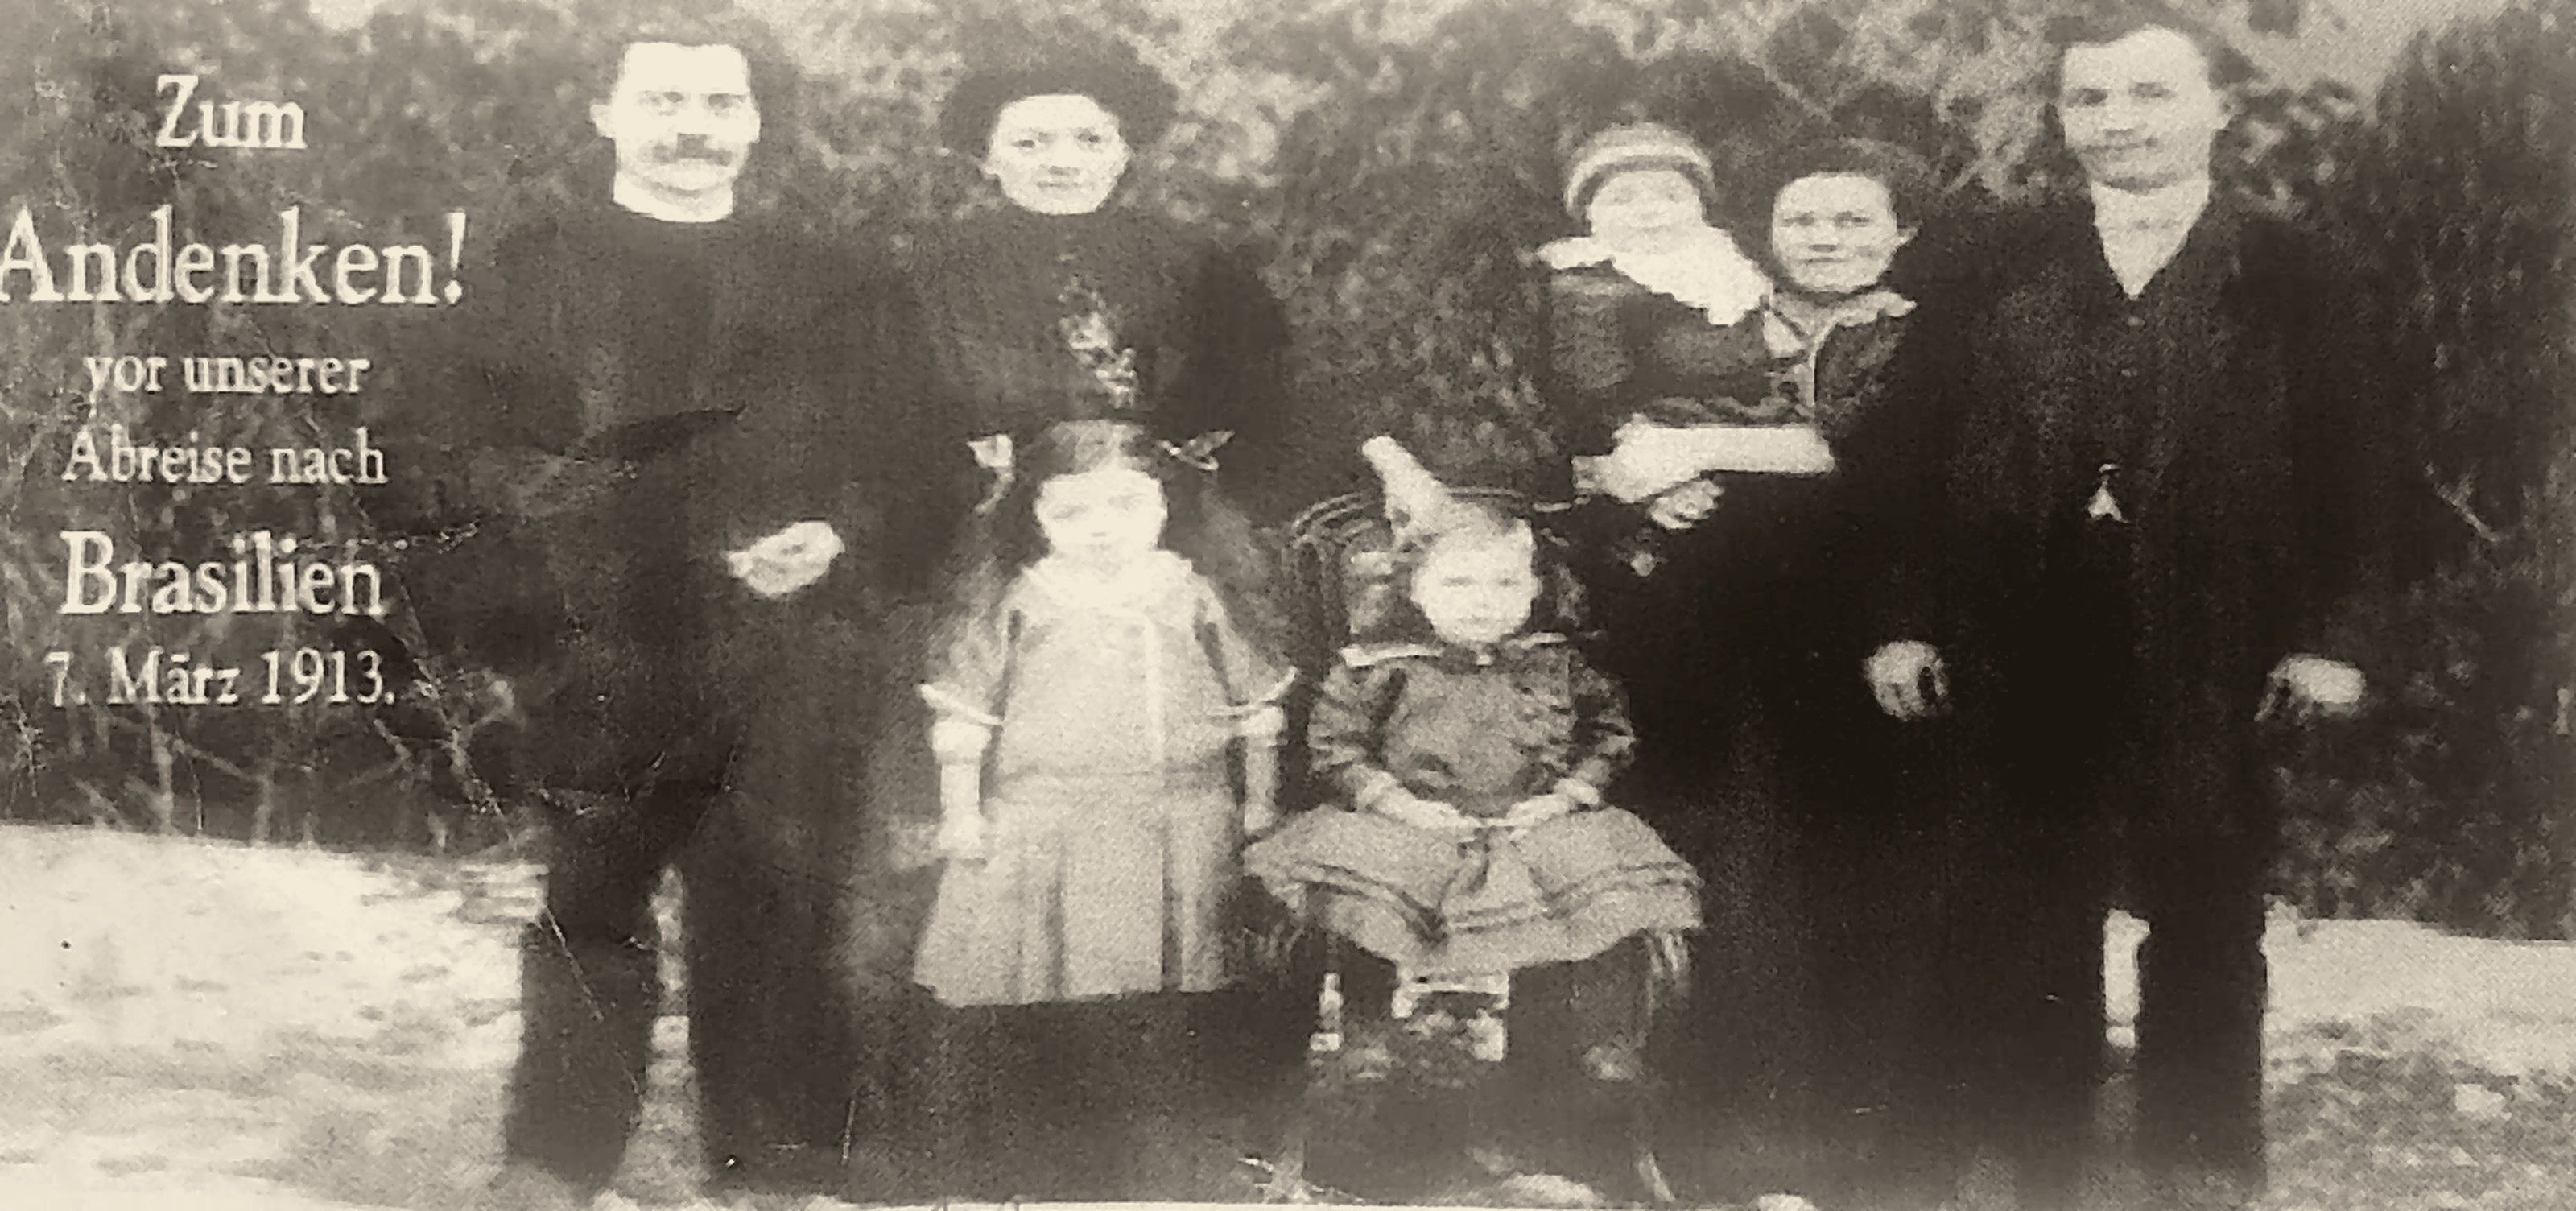
\includegraphics[width=0.95\linewidth,height=\textheight,keepaspectratio,alt={„Zum Andenken! vor unserer Abreise nach Brasilien, 7. März 1913.`` Abschiedsfoto, sehr wahrscheinlich in Deutschland vor der Reise nach Brasilien aufgenommen. Rechts die Mota mit Walter auf dem Arm und der Fata; in der Mitte Luisa und ein weiteres Kind; links ein noch nicht identifiziertes Paar aus der Verwandtschaft. Familienbesitz. Kontrast und Rauschen vom Autor korrigiert.}]{imagens/haas_despedida_abreise_brasilien_1913_restaurada.jpg}
\caption{\emph{„Zum Andenken! vor unserer Abreise nach Brasilien, 7.
März 1913.``} Abschiedsfoto, sehr wahrscheinlich in Deutschland vor der
Reise nach Brasilien aufgenommen. Rechts die Mota\index[pessoas]{meier, maria@Meier, Maria} mit Walter auf dem Arm
und der Fata\index[pessoas]{haas, johann@Haas, Johann}; in der Mitte Luisa\index[pessoas]{haas, luisa@Haas, Luisa} und ein weiteres Kind; links ein noch
nicht identifiziertes Paar aus der Verwandtschaft. Familienbesitz.
Kontrast und Rauschen vom Autor korrigiert.}
\end{figure}

Sieben Menschen stehen auf dem Bild, auf hellem Boden: festgetretene
Erde, vielleicht alter Schnee, das ist nicht zu sagen. Links ein Mann
mit Schnurrbart in dunkler Kleidung, die Hände vor dem Körper gefaltet.
Neben ihm eine Frau mit hochgestecktem Haar, ebenfalls in Dunkel. Rechts
eine Frau, die ein Baby mit Häubchen auf dem Arm hält, und neben ihr ein
junger Mann ohne Schnurrbart in zugeknöpfter Jacke. Zwischen den
Erwachsenen zwei Kinder: ein stehendes Mädchen in hellem Kleid mit einer
Schleife im Haar und ein kleineres Kind, das in einem Rüschenkleid auf
einem Korbstühlchen sitzt.

Ich habe lange auf dieses Bild geschaut, und jahrelang hat es mir mehr
Fragen als Antworten gegeben. Entschlüsselt hat es das Gedächtnis der
Familie: Die Frau mit dem Baby auf dem Arm ist die Mota\index[pessoas]{meier, maria@Meier, Maria}, und der junge
Mann ohne Schnurrbart neben ihr ist der Fata\index[pessoas]{haas, johann@Haas, Johann}. Johann war achtundzwanzig,
Maria vierundzwanzig. Das Baby mit dem Häubchen muss Walter sein, ein
Jahr alt, wie die Passagierliste sagt. Luisa\index[pessoas]{haas, luisa@Haas, Luisa}, zwei Jahre alt, ist eines
der beiden Kinder in der Mitte, das stehende Mädchen oder das Kind auf
dem Korbstühlchen. Das andere Kind gehört also nicht zu ihnen, und das
Paar links, der Mann mit Schnurrbart und die Frau mit dem hochgesteckten
Haar, sind die Verwandten, die zurückblieben.

Wer waren sie? Das ist die Frage, die mich jetzt nicht mehr loslässt.
Eine Schwester der Mota\index[pessoas]{meier, maria@Meier, Maria} mit ihrem Mann und einem kleinen Kind, oder ein
Bruder des Fata\index[pessoas]{haas, johann@Haas, Johann} mit seiner Frau? 1971 schrieb eine Schwester der Mota\index[pessoas]{meier, maria@Meier, Maria}
aus Rempesgrün\index[lugares]{rempesgrun@Rempesgrün}, sie habe den Abschied am Bahnhof nie vergessen, als sie
die Schwester zum letzten Mal sah (Kapitel 7). War sie die Frau links,
zwei Schritte von ihrer Schwester entfernt, wenige Tage vor dem Zug?

Eine Frage, die ich mir oft gestellt habe, ist, ob das Foto nicht in
Marseille\index[lugares]{marseille@Marseille} aufgenommen wurde, am Kai, am Tag vor der Einschiffung. Der
Kalender ließe es zu: Die \emph{Formosa} kam am 26. März in Rio an, und
die Überfahrt dauerte etwas mehr als zwei Wochen, das Schiff muss also
um den 8. bis 10. März ausgelaufen sein. Das Foto selbst zieht aber in
die andere Richtung. Der Boden ist weiß, von Schnee oder Reif, was in
Marseille\index[lugares]{marseille@Marseille} im März selten ist, und im Hintergrund stehen Kiefern- und
Tannensträucher wie in den Wäldern Sachsens und der Oberpfalz\index[lugares]{oberpfalz@Oberpfalz}. Die
Inschrift sagt \emph{vor unserer Abreise}, und sie war für die bestimmt,
die blieben. Dafür musste man entwickeln, Abzüge machen und sie
übergeben, und ein Auswanderer der dritten Klasse auf der Durchreise in
Marseille\index[lugares]{marseille@Marseille} hätte dafür weder Zeit noch Geld gehabt. Am wahrscheinlichsten
ist das Foto in Deutschland entstanden, in den letzten Tagen zu Hause.
Und dieses Zuhause lag, wie ich meine, im Vogtland\index[lugares]{vogtland@Vogtland}: derselbe
Fichtenhintergrund wie auf dem Hochzeitsfoto und dem Familienfoto im
Wäldchen (Kapitel 4), dieselbe höher gelegene, kältere Gegend, in der
die Schwestern der Mota\index[pessoas]{meier, maria@Meier, Maria} lebten und in der Anfang März noch Schnee lag.

Die Familie der Mota\index[pessoas]{meier, maria@Meier, Maria} ist auf einem anderen Foto festgehalten, dem aus
Kapitel 4, aufgenommen in einem Wäldchen, mit einem älteren Paar in der
Mitte und jungen Leuten und Kindern ringsum. Ich habe die Gesichter der
beiden Fotos nebeneinandergestellt.

\begin{figure}
\centering
\includegraphics[width=0.95\linewidth,height=\textheight,keepaspectratio,alt={Oben die vier Erwachsenen des Abschiedsfotos von 1913: die Frau links, die Mota mit Walter auf dem Arm, der Mann mit Schnurrbart und der Fata. Darunter die Gesichter vom Foto der Familie der Mota aus Kapitel 4: die beiden jungen Frauen, die hinten stehen, die junge Frau in weißer Bluse, das Mädchen links, die sitzende ältere Frau, der sitzende Mann mit Schnurrbart links, der sitzende ältere Herr und der junge Mann rechts.}]{imagens/rostos_despedida_1913_e_familia_meier.jpg}
\caption{Oben die vier Erwachsenen des Abschiedsfotos von 1913: die Frau
links, die Mota\index[pessoas]{meier, maria@Meier, Maria} mit Walter auf dem Arm, der Mann mit Schnurrbart und der
Fata\index[pessoas]{haas, johann@Haas, Johann}. Darunter die Gesichter vom Foto der Familie der Mota\index[pessoas]{meier, maria@Meier, Maria} aus Kapitel
4: die beiden jungen Frauen, die hinten stehen, die junge Frau in weißer
Bluse, das Mädchen links, die sitzende ältere Frau, der sitzende Mann
mit Schnurrbart links, der sitzende ältere Herr und der junge Mann
rechts.}
\end{figure}

Ich kann mit diesen Bildern nichts behaupten, und ich misstraue jedem,
der es tut. Die Kopie von 1913 ist so körnig, dass ein Gesicht zu einem
hellen Fleck mit zwei dunklen Punkten wird. Trotzdem: Schaut in Ruhe
hin. Der Mann mit Schnurrbart von 1913 hat dieselbe Gesichtsform wie der
Mann mit Schnurrbart, der auf dem Foto aus dem Wäldchen links sitzt.
Wenn es derselbe Mann ist, war er auf beiden Fotos der Familie der Mota\index[pessoas]{meier, maria@Meier, Maria}:
sehr wahrscheinlich ein Schwiegersohn der Meiers, verheiratet mit einer
der Schwestern. Dann wäre die Frau links auf dem Bild von 1913 diese
Schwester. Auch der junge Mann, der auf dem Foto aus dem Wäldchen rechts
sitzt, erinnert an den Fata\index[pessoas]{haas, johann@Haas, Johann} von 1913. Das ältere Paar wären Georg Adam
und Franziska, beide um die fünfzig, und der Junge mit Krawatte, etwa
acht Jahre alt und lange nach 1892 geboren, könnte der Karl\index[pessoas]{meier, karl@Meier, Karl} aus den
Briefen sein. Das sind viele „Wenn``. Das überlasse ich euch, und den
Verwandten in Rempesgrün\index[lugares]{rempesgrun@Rempesgrün}, falls sie diese Fotos eines Tages mit uns
ansehen.

Was das Foto ohne jede Zweideutigkeit aussagt, sind das Datum und die
Absicht. Am 7. März 1913 wusste jemand, dass er nach Brasilien
aufbrechen würde, und wollte, dass die Zurückbleibenden eine Erinnerung
hatten. Im Wort \emph{Andenken} steckt \emph{denken}: Es ist das, was
einen an jemanden denken lässt. Das Foto war dafür gemacht, von denen
angeschaut zu werden, die blieben. Es ist eine schöne Ironie, dass es
den Ozean überquert hat und zu uns gelangt ist, zu denen, die gingen.

\section{Zeilen 161 bis 164}\label{zeilen-161-bis-164}

\emph{Marseille\index[lugares]{marseille@Marseille}, März 1913}

Die meisten deutschen Auswanderer fuhren von Hamburg oder Bremen ab, den
großen Nordseehäfen. Die Haas fuhren von Marseille\index[lugares]{marseille@Marseille} ab. Die Erklärung,
die ich von meinem Vater hörte, lautet: 1913 habe die deutsche Regierung
in Erwartung des Krieges die Auswanderung verboten, und deshalb sei die
Familie über einen Hafen außerhalb Deutschlands ausgereist. Johann war
28, im wehrpflichtigen Alter. Das Gesetz, das dies bestätigt, habe ich
noch nicht gefunden, und ich muss herausfinden, ob es ein allgemeines
Verbot gab oder Beschränkungen für Männer im wehrfähigen Alter. Andere
Gründe können mitgespielt haben: eine billigere Überfahrt bei einer
französischen Reederei oder ein Auswanderungsagent, der mit den
Mittelmeerschiffen zusammenarbeitete.

Die Geschichte hat eine Folge für euch. Weil sie auf diese Weise
ausgereist war, hielt die Familie es für unmöglich, die deutsche
Staatsangehörigkeit zu bekommen. Nur hat der Fata\index[pessoas]{haas, johann@Haas, Johann} die seine nie
aufgegeben. Er lebte in Brasilien als Ausländer und ging von Zeit zu
Zeit zur Polícia Federal, der Bundespolizei, bei der sich Ausländer
melden mussten, um sich registrieren zu lassen. Wenn die Papiere das
bestätigen, kann die Staatsangehörigkeit vom Vater auf den Sohn bis zu
euch weitergegeben worden sein. Ich bin kein Anwalt: Die Antwort hängt
von den deutschen Gesetzen der damaligen Zeit und von den Dokumenten ab,
und entscheiden wird die deutsche Behörde. Aber es ist eine Tür, die
offen sein könnte, und der Fata\index[pessoas]{haas, johann@Haas, Johann} selbst hat sie so hinterlassen.

Ich stelle mir die Zugfahrt vor: von Bayern\index[lugares]{bayern@Bayern} nach Südwesten, über die
französische Grenze, das Rhonetal hinunter. Ich stelle mir den Moment
vor, in dem sich die Luft veränderte. Wer Anfang März aus dem
kontinentalen bayerischen Winter kommt und Marseille\index[lugares]{marseille@Marseille} erreicht, findet
eine andere Welt: Mittelmeerlicht, Olivenbäume und vielleicht den
Mistral, den kalten, trockenen Wind, der das Rhonetal herabweht und in
Böen über den Hafen fegt. Die Urgroßeltern tauschten den Böhmischen Wind
gegen den Mistral, und bald würden sie den Mistral gegen die Passatwinde
tauschen. So zeichne ich, aus Berufsgewohnheit, ihre Route als eine
Folge von Winden.

Im Hafen der Dampfer \emph{Formosa}. Und an Bord eine Liste.

\begin{figure}
\centering
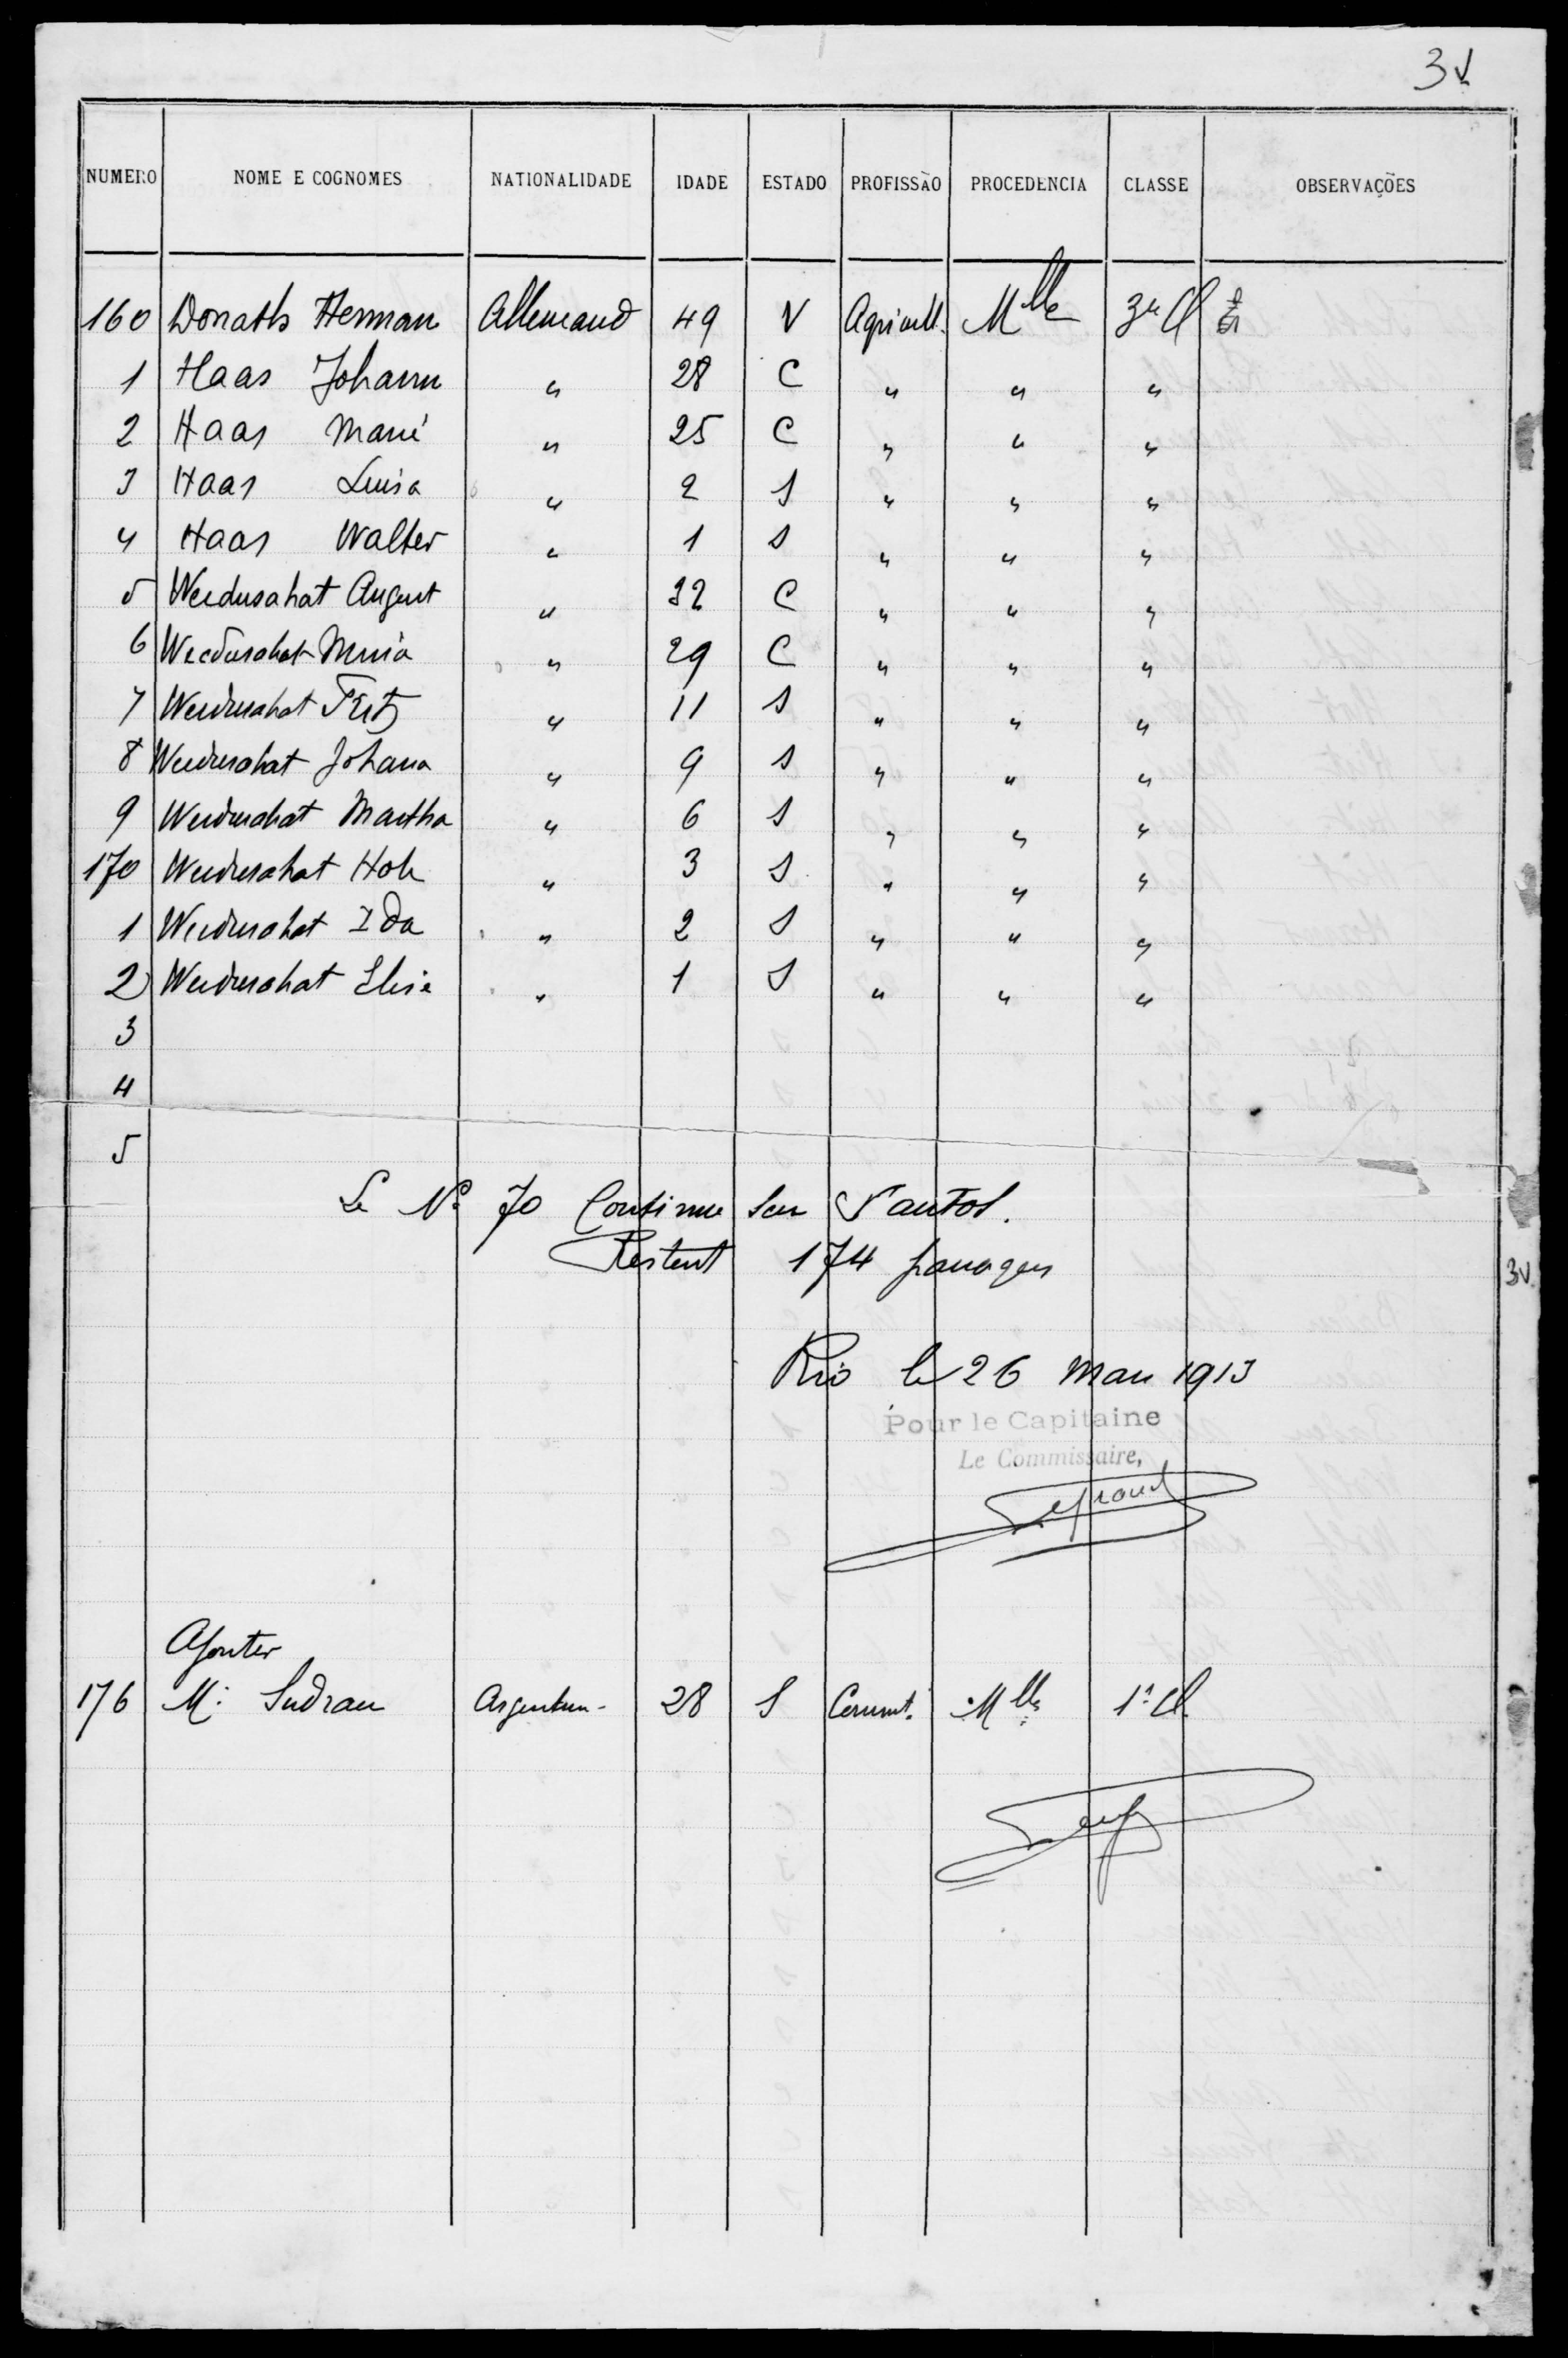
\includegraphics[width=0.9\linewidth,height=\textheight,keepaspectratio,alt={Passagierliste des Dampfers Formosa, Blatt 31, mit der Familie Haas in den Zeilen 161 bis 164: Johann, 28 Jahre; Marie, 25; Luisa, 2; Walter, 1. Unten der Vermerk „Le Nº 70 continue sur Santos. Restent 174 passagers`` und das Datum „Rio, le 26 Mars 1913``.}]{imagens/doc_haas_navio_formosa_1913.jpg}
\caption{Passagierliste des Dampfers \emph{Formosa}, Blatt 31, mit der
Familie Haas in den Zeilen 161 bis 164: Johann, 28 Jahre; Marie, 25;
Luisa\index[pessoas]{haas, luisa@Haas, Luisa}, 2; Walter, 1. Unten der Vermerk „Le Nº 70 continue sur Santos.
Restent 174 passagers`` und das Datum „Rio, le 26 Mars 1913``.}
\end{figure}

\begin{ficha}

\textbf{Archivkarte}: Passagierliste des Dampfers \emph{Formosa} aus
Marseille\index[lugares]{marseille@Marseille}, vorgelegt in Rio de Janeiro\index[lugares]{rio de janeiro@Rio de Janeiro}. Blatt Nummer 31. Gedruckte
Spaltenköpfe auf Portugiesisch (\emph{Numero, Nome e Cognomes,
Nationalidade, Idade, Estado, Profissão, Procedencia, Classe,
Observações}), handschriftlich auf Französisch ausgefüllt. Zeilen 161
bis 164: \emph{Haas Johann}, 28, \emph{C} (verheiratet); \emph{Haas
Marie}, 25, \emph{C}; \emph{Haas Luisa\index[pessoas]{haas, luisa@Haas, Luisa}}, 2, \emph{S} (ledig); \emph{Haas
Walter}, 1, \emph{S}. Staatsangehörigkeit \emph{Allemand}, Beruf
\emph{Agricult.}, Herkunft \emph{M\textsuperscript{lle}} (Marseille\index[lugares]{marseille@Marseille}) und
\emph{3\textsuperscript{e} Cl.} (dritte Klasse), alles ab Zeile 160
durch Wiederholungszeichen angegeben. Vermerk unten: \emph{„Le Nº 70
continue sur Santos. Restent 174 passagers.``} Datum und Unterschrift:
\emph{„Rio, le 26 Mars 1913. Pour le Capitaine, Le Commissaire``}. Bild:
\texttt{imagens/doc\_haas\_navio\_formosa\_1913.jpg}.

\end{ficha}

Als ich dieses Dokument zum ersten Mal sah, war das Gefühl ähnlich, wie
wenn man in einer Datenreihe, die man für verloren hielt, eine saubere
Beobachtung findet, mit Uhrzeit und Koordinate. Bis dahin hatten wir von
der Reise 1913 nur mündliche Erinnerung, viele Male weitererzählt.
Plötzlich gab es ein Papier, geschrieben von jemandem außerhalb der
Familie, im selben Jahr, und es sagte: Sie waren hier.

Das Papier sagt Dinge, die die Erinnerung nicht sagte. Es sagt, dass
Johann sich als \emph{agriculteur}, als Landwirt, angab und nicht als
Stuckateur, was völlig einleuchtet, denn Brasilien wollte Siedler für
den Ackerbau, nicht städtische Handwerker, und wahrscheinlich hatte der
Auswanderungsagent allen geraten, sich so einzutragen. Es sagt, dass
Maria fünfundzwanzig war, während sie im März 1913 in Wahrheit noch
vierundzwanzig war: Fünfundzwanzig wurde sie erst am 7. April, schon auf
der brasilianischen Seite des Ozeans. Ein kleiner Unterschied, von der
Art, die am Schalter aufgerundet wird. Es sagt, dass sie dritter Klasse
reisten, wie fast alle Auswanderer. Und es sagt ohne jede
Zweideutigkeit, dass Luisa\index[pessoas]{haas, luisa@Haas, Luisa}, zwei Jahre alt, und Walter, ein Jahr alt, an
Bord waren.

Weiter unten auf demselben Blatt steht eine ganze Familie mit schwer
lesbarem Nachnamen (etwa \emph{Weidushat}), Vater, Mutter und sechs
Kinder von elf Jahren abwärts. Ich denke an die Gespräche in der dritten
Klasse zwischen Maria und jener anderen Mutter mit sechs Kindern. Ich
weiß nichts über sie. Ich weiß, dass sie sich dieselbe Seite teilten und
wahrscheinlich dasselbe Zwischendeck.

Wie die Überfahrt war, weiß ich auch nicht. Siebzehn oder achtzehn Tage
vielleicht, von Marseille\index[lugares]{marseille@Marseille} nach Rio: das Mittelmeer, die Straße von
Gibraltar, die afrikanische Küste, die äquatorialen Kalmen, der
Südostpassat. Für eine Frau, die vielleicht schwanger war und sich im
Zwischendeck der dritten Klasse um ein einjähriges Kind und ein
zweijähriges Mädchen kümmerte, war wohl jeder dieser Tage lang. Ich
werde keine Stürme erfinden. Die Reanalyse für 1913 ist zu grob, um mir
zu sagen, was die \emph{Formosa} erlebt hat, und mir ist ehrliches
Schweigen lieber als erfundenes Drama.

Ich weiß, dass sie am 26. März in Rio ankamen. Das Manifest sagt es.

\begin{figure}
\centering
\includegraphics[width=0.85\linewidth,height=\textheight,keepaspectratio,alt={Die Reise von 1913, von Marseille nach Rio de Janeiro. Der Verlauf ist schematisch: Ich kenne weder die Route noch die Zwischenhäfen dieser Reise, und der Ort der Ankunft in Santa Catarina ist weiterhin offen. Karte des Autors.}]{imagens/mapa_viagem_1913.jpg}
\caption{Die Reise von 1913, von Marseille nach Rio de Janeiro. Der
Verlauf ist schematisch: Ich kenne weder die Route noch die
Zwischenhäfen dieser Reise, und der Ort der Ankunft in Santa Catarina
ist weiterhin offen. Karte des Autors.}
\end{figure}

\section{Was das Papier sagt und was es nicht
sagt}\label{was-das-papier-sagt-und-was-es-nicht-sagt}

\emph{Rio de Janeiro\index[lugares]{rio de janeiro@Rio de Janeiro}, 26. März 1913}

Viele Jahre lang erzählte die Familie die Ankunft nur auf eine Weise.
Der Jubiläumstext, den Marise\index[pessoas]{lourenco, marise haas@Lourenço, Marise Haas} 2013 schrieb, hielt diese Fassung fest:
Die Ausschiffung in Rio sei verweigert worden, das Schiff sei von Hafen
zu Hafen die Küste entlanggefahren und habe Quarantäne gehalten, mit zu
vielen Menschen, schlechtem Essen und „unzähligen Todesfällen`` an Bord,
bis die Familie erschöpft in Laguna\index[lugares]{laguna@Laguna} an Land ging.

Ich muss euch gegenüber deutlich sein, denn die ersten Fassungen dieses
Buches stützten sich zu sehr auf diesen Text. Er wurde hundert Jahre
nach den Ereignissen geschrieben, aus Erinnerungen aus dritter und
vierter Hand, um auf einem Fest vorgelesen zu werden. Er hat das große
Verdienst, zusammengetragen zu haben, was die Familie wusste. Aber wo er
sich mit Dokumenten vergleichen lässt, irrt er häufig. Deshalb ist die
Regel dieses Buches einfach: \textbf{Wenn das zeitgenössische Papier und
die Überlieferung sich widersprechen, halte ich mich an das Papier}, und
die Überlieferung wird zur Frage, nicht zur Antwort.

Das zeitgenössische Papier ist in diesem Punkt die Liste der
\emph{Formosa}. Sie wurde am 26. März 1913 in Rio de Janeiro\index[lugares]{rio de janeiro@Rio de Janeiro} vom
Zahlmeister des Schiffes unterschrieben, um den brasilianischen Behörden
übergeben zu werden. Darin stehen lebend, in den Zeilen 161 bis 164, die
vier Haas: Johann, Marie, Luisa\index[pessoas]{haas, luisa@Haas, Luisa} und Walter. Niemand aus der Familie ist
auf der Überfahrt gestorben. Die Spalte für Bemerkungen, in die ein
Todesfall an Bord eingetragen worden wäre, ist leer. Der Vermerk unten
auf der Seite (\emph{„Le Nº 70 continue sur Santos. Restent 174
passagers``}) besagt, dass ein Passagier nach Santos weiterfuhr und die
übrigen blieben. Rio war der Ankunftshafen der Familie. Kein Dokument,
das ich gesehen habe, spricht von einer verweigerten Ausschiffung, von
einem Schiff, das die Küste entlangirrte, oder von Toten an Bord.

Was das Papier nicht sagt, ist, was danach kam. Die Neuankömmlinge
durchliefen in der Regel die Einwandererherberge auf der Ilha das Flores
in der Guanabara-Bucht und wurden von dort in die Zielstaaten
weitergeschickt. Die Register der Ilha das Flores und der
Einwanderungsinspektion, die im brasilianischen Nationalarchiv (Arquivo
Nacional) liegen, müssten sagen, wann die Haas Rio verließen, auf
welchem Schiff und in welchen Hafen von Santa Catarina. Es kann
Florianópolis\index[lugares]{florianopolis@Florianópolis} gewesen sein, wo Vetter Agenor\index[pessoas]{haas, agenor@Haas, Agenor} gesucht hat, ohne etwas zu
finden, oder Laguna\index[lugares]{laguna@Laguna}, wie die Überlieferung sagt. Solange diese Bücher
nicht aufgeschlagen sind, weiß ich es nicht. Und ich werde die Lücke
nicht mit Quarantänen und Stürmen füllen.

\section{Gertrudes}\label{gertrudes}

Dasselbe gilt für die Geburt von Gertrudes. Die Überlieferung sagt, sie
sei am 5. Mai 1913 in der Einwandererbaracke von Laguna\index[lugares]{laguna@Laguna} geboren, dem
Barracão dos Imigrantes. Die Tabelle von Vetter Agenor\index[pessoas]{haas, agenor@Haas, Agenor} sagt, sie sei am
22. Oktober 1911 in Deutschland geboren und mit dem Schiff gekommen. Das
Manifest führt keine Gertrudes an Bord, und schon das machte das Datum
1911 schwer haltbar: Ein sechzehn Monate altes Mädchen stünde auf der
Liste, so wie die einjährigen Kinder auf derselben Seite.

Das fehlende Papier tauchte in den Indizes der katholischen
Kirchenbücher von Santa Catarina auf. Gertrud, Tochter von Johann Haas\index[pessoas]{haas, johann@Haas, Johann}
und Maria Meyer, wurde am 23. November 1913 in der Pfarrei Teresópolis
getauft, heute Águas Mornas\index[lugares]{aguas mornas@Águas Mornas}, die die Kolonie Anitápolis\index[lugares]{anitapolis@Anitápolis} betreute. Ihr
Profil bei FamilySearch gibt als Geburt den 5. Mai 1913 in Anitápolis\index[lugares]{anitapolis@Anitápolis}
an. Das Datum der Überlieferung stimmte; der Ort wahrscheinlich nicht.
Gertrudes wurde etwa sechs Wochen nach der Ankunft in Rio geboren, Maria
reiste also schwanger, wie die Familie es immer erzählt hat. Gertrudes
wuchs heran, heiratete im Mai 1932 in Ituporanga\index[lugares]{ituporanga@Ituporanga} Augusto Sebold, einen
Sohn von Siedlern aus Teresópolis, und ging mit ihm in den Norden von
Paraná. Sie starb am 23. Juni 1997 in Pindauvinha, Gemeinde Ivaiporã.

\begin{ficha}

\textbf{Archivkarte}: Taufe von Gertrud Haas, Tochter von Johann Haas\index[pessoas]{haas, johann@Haas, Johann}
und Maria Meyer, am 23.11.1913, Pfarrei Teresópolis (SC): „Brasil, Santa
Catarina, Registros da Igreja Católica, 1714--1977``, FamilySearch,
ark:/61903/1:1:QPQC-X62B. Heirat mit Augusto Sebold: kirchlich am
07.05.1932 und standesamtlich am 09.05.1932, Ituporanga\index[lugares]{ituporanga@Ituporanga} („Brasil, Santa
Catarina, Registro Civil, 1850--1999``, ark:/61903/1:1:X9B4-G1T4).
Geburtsdatum (05.05.1913, Anitápolis\index[lugares]{anitapolis@Anitápolis}) und Sterbedatum (23.06.1997,
Pindauvinha, Ivaiporã, PR) stammen aus dem Profil G8P8-X9D, bisher ohne
beigefügte Urkunde.

\end{ficha}

\section{Wo Luisa und Walter sind}\label{wo-luisa-und-walter-sind}

Auch über die beiden Kinder der \emph{Formosa} hat sich die schriftliche
Überlieferung geirrt. Der Jubiläumstext sagt, Luisa\index[pessoas]{haas, luisa@Haas, Luisa} und Walter seien
noch in den Baracken gestorben, geschwächt von der Reise. Agenors
Tabelle verzeichnet jedoch zwei Kinder, „Lina`` und „Valter``, begraben
in Rio do Ouro\index[lugares]{rio do ouro@Rio do Ouro}, Anitápolis\index[lugares]{anitapolis@Anitápolis}, dem Ort, an den die Familie nach der Ankunft
zog. Und es gibt einen Zeugen, den ich mit eigenen Ohren gehört habe:
meinen Vater.

Baldoíno erzählte mir, er sei mit seinen Geschwistern nach Anitápolis\index[lugares]{anitapolis@Anitápolis}
gefahren, um die sterblichen Überreste der kleinen Geschwister zu holen
und nach Ituporanga\index[lugares]{ituporanga@Ituporanga} zu bringen. Auf dieser Reise, oben im Gebirge, sah
er zum ersten Mal Schnee. Walter liegt heute in Ituporanga\index[lugares]{ituporanga@Ituporanga} begraben, bei
der Familie. Die Kinder haben die Reise also überlebt, sind in Rio do
Ouro angekommen und dort gestorben. Jahre später holten die Geschwister
sie.

„Lina`` ist sehr wahrscheinlich die Luisa\index[pessoas]{haas, luisa@Haas, Luisa} der Bordliste, unter ihrem
Rufnamen im Haus; „Valter`` ist Walter in brasilianischer Schreibweise.
Ich kenne noch nicht die Sterbedaten, nicht das Jahr der Umbettung und
nicht den Winter, in dem es im Gebirge schneite, sodass mein Vater den
Schnee sehen konnte. Aber die Geschichte steht jetzt auf drei Beinen:
einem Papier von Bord, einer sorgfältig angelegten Tabelle und dem
Bericht dessen, der die Überreste getragen hat. Sie hängt nicht mehr an
einem Satz, der für ein Fest geschrieben wurde.

Der Rest bleibt offen. Das Abreisedatum, das Agenor\index[pessoas]{haas, agenor@Haas, Agenor} notiert hat, der 13.
März, passt weder zum Foto vom 7. März noch zur Ankunft in Rio am 26.
Das Foto kann den Abschied zu Hause markieren und nicht die Einschiffung
in Marseille\index[lugares]{marseille@Marseille}; die Zugfahrt bis Frankreich dauerte Tage. Der 26. April,
ebenfalls von ihm notiert, liegt genau einen Monat nach der Ankunft in
Rio: Das kann die Ankunft in Santa Catarina sein, nach Herberge und
Küstenschiff, oder ein bloßer Irrtum im Monat. Die Taufe von Gertrudes
in Teresópolis legt nahe, dass die Familie über Florianópolis\index[lugares]{florianopolis@Florianópolis}, Palhoça
und Teresópolis nach Anitápolis\index[lugares]{anitapolis@Anitápolis} hinaufzog und nicht über Laguna\index[lugares]{laguna@Laguna}; aber
die Liste des Küstenschiffs ist noch nicht gefunden. Diese Fragen sind
am Ende dieses Buches einzeln aufgeführt, für alle, die suchen möchten.

\section{Laguna, Februar 2012}\label{laguna-februar-2012}

Im Februar 2012 fuhren wir nach Laguna\index[lugares]{laguna@Laguna} und Tubarão\index[lugares]{tubarao@Tubarão}: ich, Bárbara,
Matheus und Lucas. Matheus war neun; Lucas wurde bald sieben. Sie waren
nicht viel älter als Luisa\index[pessoas]{haas, luisa@Haas, Luisa} und Walter, als die beiden den Ozean
überquerten.

Damals hatte ich das Manifest der \emph{Formosa} noch nicht und wusste
nichts von all diesen Widersprüchen. Ich wusste, was die Familie
wiederholte: dass der Fata\index[pessoas]{haas, johann@Haas, Johann} und die Mota\index[pessoas]{meier, maria@Meier, Maria} über Laguna\index[lugares]{laguna@Laguna} gekommen waren und
dass dort die ersten Gräber der Familie in Brasilien lagen. Heute weiß
ich, dass der zweite Teil falsch ist, denn die Gräber waren in
Anitápolis\index[lugares]{anitapolis@Anitápolis}, und dass der erste noch auf ein Dokument wartet. Aber wir
sahen uns die Stadt mit diesem Gedanken im Kopf an.

Laguna\index[lugares]{laguna@Laguna} ist eine der ältesten Städte Santa Catarinas, gegründet im 17.
Jahrhundert. Die Altstadt hat portugiesische Kolonialhäuser, die
Hauptkirche Santo Antônio dos Anjos und enge Gassen, die zur Lagune
hinabführen. Es war die Heimat von Anita Garibaldi und der Schauplatz
der kurzlebigen Julianischen Republik von 1839. Es ist auch die Stadt
der Delfine, die seit Generationen die Schwärme von Meeräschen auf die
Wurfnetze der Fischer an der Hafeneinfahrt zutreiben, eine
Zusammenarbeit zwischen Arten, die Biologen bis heute erforschen. Vor
allem ist es eine Stadt, die um eine Wasserpassage herum gebaut ist: die
Barra, die Durchfahrt, die das Lagunensystem mit dem Ozean verbindet und
durch die die Schiffe ein- und ausfuhren.

Wenn die Urgroßeltern dort hereinkamen, haben sie keine Spur
hinterlassen. Es gibt keine Tafel, keinen Eintrag am Kai, keine
Gedenkstätte für die Einwandererbaracke, jedenfalls keine, die ich
gefunden hätte. Es gibt nur die Barra und das Wasser, das mit den
Gezeiten ein- und ausströmt.

In Tubarão\index[lugares]{tubarao@Tubarão}, ein paar Dutzend Kilometer flussaufwärts, sahen wir uns die
Sammlung von Willy Zumblick an, dem Maler der Stadt, der einen guten
Teil seines Lebens der Darstellung der Geschichte des südlichen Santa
Catarina widmete: Anita, Garibaldi, die Lastkähne der Julianischen
Republik, die Küstenlandschaft. Ich mag Historienmaler aus demselben
Grund, aus dem ich Reanalysen mag: Sie rekonstruieren, was niemand
fotografiert hat, und wissen, dass sie rekonstruieren.

Den Rest dieser Reise überlasse ich den Jungen und Bárbara, die ihre
eigenen Erinnerungen daran haben. Meine, die für dieses Buch zählt, ist
das Bild eines Geographen: Laguna\index[lugares]{laguna@Laguna} liegt an der Mündung eines Flusses.
Der Fluss ist der Tubarão\index[lugares]{tubarao@Tubarão}.

\section{Der Fluss, der zur Barra
hinabfließt}\label{der-fluss-der-zur-barra-hinabflieuxdft}

Wer vom Meer her nach Laguna\index[lugares]{laguna@Laguna} kommt, sieht den Tubarão\index[lugares]{tubarao@Tubarão} nicht. Er mündet
hinter der Stadt in das Lagunensystem, nachdem er von der Serra Geral
herabgekommen ist, die Stadt Tubarão\index[lugares]{tubarao@Tubarão} durchquert und sich durch die
Küstenebene geschlängelt hat. Das Wasser, das durch die Barra von Laguna\index[lugares]{laguna@Laguna}
hinausströmt, ist zu einem guten Teil Regen, der im Gebirge gefallen
ist.

Im März 1974 kam dieses Wasser auf einmal herunter.

Am 24. und 25. März 1974 verwüstete ein Hochwasser die Stadt Tubarão\index[lugares]{tubarao@Tubarão}. Es
war die bis dahin größte Naturkatastrophe in der Geschichte Santa
Catarinas. Die meistzitierten offiziellen Zahlen sprechen von etwa
zweihundert Toten und Zehntausenden Obdachlosen. Ganze Stadtviertel
standen unter Wasser; die Stadt brauchte Jahre, um sich zu erholen. Nach
der Tragödie wurde der Fluss im Stadtgebiet begradigt und kanalisiert:
Die Schleifen, die das Wasser über Jahrtausende gezeichnet hatte, wurden
von Ingenieuren durchschnitten, die das mit gutem Grund nicht noch
einmal erleben wollten.

Ich war im März 1974 acht Jahre alt. Ich dachte noch nicht daran,
Meteorologe zu werden. Wenn ich heute auf dieses Ereignis schaue, sehe
ich, was mein Beruf mich zu sehen gelehrt hat: ein Einzugsgebiet, das an
steilen Abbruchkanten entspringt, Steigungsregen empfängt, wenn feuchte
Meeresluft gegen das Gebirge gedrückt wird, dieses Wasser in wenigen
Stunden sammelt und in eine tief liegende Ebene schüttet, wo es
nirgendwohin kann als zur Seite. 1973 und 1974 befand sich der Pazifik
in einer La-Niña-Phase. Viele suchen in El Niño und La Niña gern die
Erklärung für jede Katastrophe, und hier muss ich vorsichtig sein: Diese
Schwankungen verändern die Wahrscheinlichkeiten, sie entscheiden nicht
das Schicksal. Das Klima lädt die Würfel; geworfen werden sie vom
Wetter, Tag für Tag. Eine Front, die stehen bleibt, ein Tief, das sich
vertieft, eine östliche Strömung, die einen Tag länger anhält: Das macht
aus einer Regenzeit eine Katastrophe.

Ich arbeite seit Jahren mit Hochwassermodellierung, Hydrologie und
Vorhersage. Einen guten Teil meiner Laufbahn habe ich damit verbracht
vorherzusehen, was die Flüsse Santa Catarinas tun werden, wenn der Regen
kommt: der Itajaí\index[lugares]{itajai@Itajaí}, der Tubarão\index[lugares]{tubarao@Tubarão} und auch der Taquari drüben in Rio Grande
do Sul, woher Bárbaras Familie stammt. Projekte will ich hier nicht
ausbreiten. Ich will einen Zufall festhalten, der mir erst beim
Schreiben dieses Kapitels aufgefallen ist: Die Stadt, die die Familie
immer als ihr Eingangstor bezeichnet hat, liegt an der Mündung eines
Flusses, der sechs Jahrzehnte später die größte Tragödie in der
Geschichte des Bundesstaates anrichten sollte. Und ihr Enkel würde, ohne
von dieser Verbindung zu wissen, sein Leben damit verbringen, genau
diese Art von Wasser zu erforschen.

Dieses Buch wird zu den Hochwassern zurückkehren. In Kapitel 13
erscheinen die drei Flüsse unserer Familien (der Tubarão\index[lugares]{tubarao@Tubarão}, der Itajaí\index[lugares]{itajai@Itajaí} und
der Taquari) gemeinsam, denn der Regen, der auf sie fällt, ist oft ein
und derselbe. Vorerst lasse ich nur dieses Bild stehen: die Barra von
Laguna\index[lugares]{laguna@Laguna} als Eingangstor. Durch sie kamen Einwandererschiffe herein; durch
sie geht jeden Tag der Regen aus dem Gebirge hinaus. Wenn die Haas sie
passiert haben, dann einmal, von außen nach innen. Der Fluss passiert
sie immer, von innen nach außen.

An einem Tag des Jahres 1913, den kein bisher gefundenes Papier
verzeichnet, erreichten Johann und Maria die Küste von Santa Catarina
und stiegen ins Gebirge hinauf. Sie hatten Luisa\index[pessoas]{haas, luisa@Haas, Luisa} und Walter bei sich,
die noch lebten, und früher oder später ein neugeborenes Mädchen namens
Gertrudes. Vor ihnen lagen die Hänge der Serra und das Versprechen eines
Stücks Land an einem Ort namens Rio do Ouro\index[lugares]{rio do ouro@Rio do Ouro}, Goldfluss.

Der Name war, wie so viele Namen jener Zeit, ein Versprechen, das das
Land nicht halten würde.

\section{Für euch zum Entdecken}\label{fuxfcr-euch-zum-entdecken-4}

\begin{itemize}
\tightlist
\item
  Hat Deutschland 1913 wirklich die Auswanderung verboten, wie mein
  Vater erzählte? Warum schifften sich die Haas in Marseille\index[lugares]{marseille@Marseille} ein, wenn
  die meisten deutschen Auswanderer von Hamburg oder Bremen abfuhren?
\item
  Wo sind die Ausländerkarten des Fata\index[pessoas]{haas, johann@Haas, Johann}, aus den Meldungen, die er bei
  der Polícia Federal machte? Sie könnten der Beweis sein, dass er
  Deutscher geblieben ist.
\item
  Auf welchem Schiff und über welchen Hafen kam die Familie nach Santa
  Catarina: Laguna\index[lugares]{laguna@Laguna}, Florianópolis\index[lugares]{florianopolis@Florianópolis} oder einen anderen? Die Bücher der
  Ilha das Flores und der Einwanderungsinspektion im Arquivo Nacional
  müssten es sagen.
\item
  Wer sind der Mann mit Schnurrbart und die Frau links auf dem Foto vom
  7. März, und wem gehört das Kind, das weder Luisa\index[pessoas]{haas, luisa@Haas, Luisa} noch Walter ist?
  Fragt die Vettern und Cousinen, ob es in irgendeiner Schachtel eine
  schärfere Kopie gibt.
\item
  In welchem Winter schneite es im Gebirge, als Baldoíno und seine
  Geschwister die Überreste der Kinder holten? Fragt die älteren Vettern
  und Cousinen, ob sie diese Geschichte von ihren Eltern gehört haben.
\end{itemize}

\chapter{Die Gipsengel von Rio do Ouro und die Rodungen von
Ituporanga\index[lugares]{ituporanga@Ituporanga}}\label{cap-6}

\emph{27,9° S · 49,1° W, Rio do Ouro\index[lugares]{rio do ouro@Rio do Ouro}, Anitápolis\index[lugares]{anitapolis@Anitápolis} · 27,4° S · 49,6° W,
Ituporanga\index[lugares]{ituporanga@Ituporanga}, SC}

\begin{quote}
\emph{Gips härtet in Minuten aus. Land in Generationen. Wer mit beidem
arbeitet, lernt, auf zweierlei Weise zu warten.}
\end{quote}

\section{Ein Brief aus Heumaden}\label{ein-brief-aus-heumaden}

\emph{Rio do Ouro\index[lugares]{rio do ouro@Rio do Ouro}, Santa Catarina, Ende 1914}

Irgendwann zwischen Ende 1914 und Anfang 1915 (ich kenne das Datum
nicht, und der Brief, falls es ihn noch gibt, ist nie durch meine Hände
gegangen) kam im Landesinneren von Santa Catarina ein Brief aus
Deutschland an. Er war von einer Schwester der Mota\index[pessoas]{meier, maria@Meier, Maria}. Es konnte Barbara
sein, die älteste der Mädchen, oder Margaretha, oder die kleine Anna,
die 1914 etwa sechzehn gewesen wäre. Woran sich die Familie erinnert,
ist der Inhalt: Der Krieg hatte begonnen. Sie sollten nicht versuchen
zurückzukommen.

Marise\index[pessoas]{lourenco, marise haas@Lourenço, Marise Haas} erzählt das im Jubiläumstext beiläufig, in einem Satz, der viel
verbirgt: „Auch wenn sie verzweifelt waren, unglücklich, und die Zeit
zurückdrehen wollten, konnten sie nicht mehr nach Deutschland zurück,
denn ein Brief von einer Schwester der Mutter warnte sie vor dem Beginn
des Krieges.`` \emph{Mutter}: das Wort, aus dem die brasilianischen
Enkel nach dem Gehör „Mota\index[pessoas]{meier, maria@Meier, Maria}`` gemacht haben.

Ich denke darüber nach, was dieser Satz verrät. Er verrät zunächst, dass
sie zurückwollten. Gut ein Jahr nach der Ankunft, mit zwei begrabenen
Kindern und einem Land, das nichts hergab, erwogen Johann und Maria
ernsthaft den Weg zurück. Und er verrät, dass jemand in Heumaden\index[lugares]{heumaden@Heumaden} davon
wusste: dass sie nach Hause schrieben, erzählten, was geschah, und dass
die Familie in Bayern\index[lugares]{bayern@Bayern} antwortete. Es gab noch einen Faden. Der Brief der
Schwester war zugleich die Nachricht, die diesen Faden durchschnitt, und
der Beweis, dass es ihn gab.

Ich stelle mir vor, wie Maria Johann den Brief beim Schein einer
Petroleumlampe vorliest, in einem Holzhaus mitten am Hang. Ich stelle
mir die Stille zweier Menschen vor, die gerade begreifen, dass sich die
Tür hinter ihnen geschlossen hat. Von nun an führte der einzige Weg nach
vorn, und, wie Marise\index[pessoas]{lourenco, marise haas@Lourenço, Marise Haas} sagt, „sie waren nicht allein, sie hatten
Gertrudes und viele Gefährten in derselben Lage``.

\begin{figure}
\centering
\includegraphics[width=0.9\linewidth,height=\textheight,keepaspectratio,alt={Das Santa Catarina der Familie: die Flüsse und die Orte, durch die die Zweige Haas, Dörner, Preis, Michels und Arns gekommen sind. Die Flüsse stammen aus meinem Hochwassermodell. Karte des Autors.}]{imagens/mapa_santa_catarina.jpg}
\caption{Das Santa Catarina der Familie: die Flüsse und die Orte, durch
die die Zweige Haas, Dörner, Preis, Michels und Arns gekommen sind. Die
Flüsse stammen aus meinem Hochwassermodell. Karte des Autors.}
\end{figure}

\section{Lote 17}\label{lote-17}

\emph{Rio do Ouro\index[lugares]{rio do ouro@Rio do Ouro}, Kolonie Anitápolis\index[lugares]{anitapolis@Anitápolis}, 1913 bis 1918}

Von der Küste aus, über einen Hafen, den ich noch nicht kenne, zog die
Familie ins Landesinnere, die Hänge der Serra Geral hinauf, an einen Ort
namens Rio do Ouro\index[lugares]{rio do ouro@Rio do Ouro}. Heute gehört Rio do Ouro zur Gemeinde Anitápolis\index[lugares]{anitapolis@Anitápolis}, im
Bergland südwestlich des Großraums Florianópolis\index[lugares]{florianopolis@Florianópolis}. Damals gehörte es zu
Palhoça; so verzeichnet Vetter Agenor\index[pessoas]{haas, agenor@Haas, Agenor} die Geburt seines Vaters
Alexandre: „in Rio do Ouro\index[lugares]{rio do ouro@Rio do Ouro}, Palhoça, gehört heute zu Anitápolis\index[lugares]{anitapolis@Anitápolis}``.

\begin{ficha}

\textbf{Archivkarte}: Genealogische Tabelle von Agenor\index[pessoas]{haas, agenor@Haas, Agenor} Haas,
biographische Notiz zu Alexandre Haas: \emph{„geboren am 23. Mai 1917 in
Rio do Ouro\index[lugares]{rio do ouro@Rio do Ouro}, Palhoça, gehört heute zu Anitápolis\index[lugares]{anitapolis@Anitápolis}, SC, war Maurer``}. In
der Notiz über die Stammeltern vermerkt Agenor\index[pessoas]{haas, agenor@Haas, Agenor}, Johann \emph{„lebte bis
1918 im Ort Rio do Ouro\index[lugares]{rio do ouro@Rio do Ouro} in Anitápolis\index[lugares]{anitapolis@Anitápolis}, SC, und zog dann nach Rio Novo\index[lugares]{rio novo@Rio Novo} in
Ituporanga\index[lugares]{ituporanga@Ituporanga}``}. Quelle: Abschrift der ursprünglichen
\texttt{.xls}-Tabelle, aufbewahrt im privaten Familienarchiv.

\end{ficha}

Anitápolis\index[lugares]{anitapolis@Anitápolis} war eine Siedlungskolonie, die die Bundesregierung wenige
Jahre zuvor an den Oberläufen von Flüssen, die aus dem Gebirge kommen,
für europäische Einwanderer angelegt hatte. Der Name ehrte Anita
Garibaldi, die Heldin von Laguna\index[lugares]{laguna@Laguna}. Diese Wendung gefällt mir: Wenn die
Überlieferung stimmt, kam die Familie über Anitas Heimat nach Santa
Catarina und lebte dann an dem Ort, der nach ihr benannt war. Später, ab
1918, sollten die Gebäude der Kolonie ein Patronato Agrícola
beherbergen, eine landwirtschaftliche Internatsschule für arme Jungen
und Waisen, die die Regierung zu Landarbeitern machen wollte.\footnote{Zum
  Patronato Agrícola von Anitápolis\index[lugares]{anitapolis@Anitápolis} (1918--1930) siehe Daniel Alves
  Boeira, \emph{Uma ``solução'' para a menoridade na Primeira República:
  o caso do Patronato Agrícola de Anitápolis\index[lugares]{anitapolis@Anitápolis}/SC (1918--1930)},
  Masterarbeit, UDESC, 2012, zitiert von Juliana da Silva Monteiro und
  Maria do Carmo Brazil in der \emph{Revista HISTEDBR On-line}, Bd. 19,
  2019.} Aber das war schon nach dem Weggang der Haas.

Marise\index[pessoas]{lourenco, marise haas@Lourenço, Marise Haas} erzählt: „Zusammen mit einem Freund kauften sie ein Stück Land.
Das Lote 17, in Rio do Ouro\index[lugares]{rio do ouro@Rio do Ouro}.`` Ein \emph{lote} war eine der vermessenen
Parzellen, in die man das Kolonieland aufteilte und an die Siedler
verkaufte. Ich weiß nicht, wer der Freund war: ein anderer Einwanderer
aus der Baracke vielleicht, jemand von derselben Reise. Der gemeinsame
Kauf sagt viel darüber, wie wenig sie hatten: nicht einmal genug für
eine ganze Parzelle. Und das Land, schreibt Marise\index[pessoas]{lourenco, marise haas@Lourenço, Marise Haas}, war „ein undankbarer
Boden: trocken und sauer, nicht imstande, genug Nahrung hervorzubringen,
nicht einmal für den eigenen Bedarf. Bis sie herausfanden, wie
unfruchtbar er war, hatten sie das Wenige, das sie besaßen, schon
hineingesteckt.``

Bei diesem Satz will ich verweilen, denn er sagt etwas über Bodenkunde
und über Siedlungspolitik. Die Böden an den Hängen der Serra Geral in
Santa Catarina, aus altem Gestein entstanden und über Jahrtausende von
reichlichem Regen ausgewaschen, sind meist sauer und nährstoffarm. Unter
dem atlantischen Regenwald, der Mata Atlântica, täuschen sie: Der Wald
wirkt üppig, weil er seine eigenen Nährstoffe wiederverwertet; die
fallenden Blätter ernähren die Wurzeln. Ist der Wald gerodet und das
Reisig verbrannt, zehren die ersten Ernten von der Asche; nach zwei,
drei Jahren ist der Boden erschöpft. Ein erfahrener Bauer aus Bayern\index[lugares]{bayern@Bayern}, an
einen anderen Boden und ein anderes Klima gewöhnt, konnte das nicht im
Voraus wissen. Ein Stuckateur aus der Stadt noch weniger. Und Maria, die
sich mit dem Land auskannte, kannte das Land von Heumaden\index[lugares]{heumaden@Heumaden}.

Auch die Versprechungen wurden nicht gehalten. Marise\index[pessoas]{lourenco, marise haas@Lourenço, Marise Haas} zählt auf, was die
Regierung versprochen und nicht geliefert hatte: Zuschüsse in Geld,
Werkzeug, Saatgut, Vieh, Baumaterial, Straßen, Investitionen in die
Gegend. Das ist ein Kehrreim, der fast mit denselben Worten wiederkehren
wird, wenn die Familie nach Ituporanga\index[lugares]{ituporanga@Ituporanga} zieht. Die Einwanderer, die
Anfang des 20. Jahrhunderts nach Brasilien kamen, wurden oft mit
Versprechen angeworben, die der brasilianische Staat nicht erfüllen
konnte (oder nicht erfüllen wollte).

Dort, auf dem Lote 17, zwischen dem Warten auf die Ernte und der
Enttäuschung über das Wenige, das sie einbrachte, begann die Familie ihr
Leben neu aufzubauen. Zwei Jungen wurden geboren: Fernando 1915 und
Alexandre am 23. Mai 1917. Nach vier verlorenen Kindern zwei Jungen, die
durchkamen. Ich versuche mir vorzustellen, was es für Maria bedeutete,
Fernando das erste Lebensjahr überstehen zu sehen, dann das zweite.
Jeder Geburtstag muss ein kleiner Sieg gewesen sein über eine Statistik,
die sie aus nächster Nähe kannte.

Hier in Rio do Ouro\index[lugares]{rio do ouro@Rio do Ouro} verortet Agenors Tabelle auch die Gräber von Lina
und Valter, auf dem Friedhof von Anitápolis\index[lugares]{anitapolis@Anitápolis}. Es sind Luisa\index[pessoas]{haas, luisa@Haas, Luisa} und Walter,
die beiden Kinder der \emph{Formosa}: Sie kamen lebend in Rio an,
stiegen mit den Eltern ins Gebirge hinauf, und erst im neuen Land
starben sie und wurden begraben. Dort blieben sie nicht für immer. Mein
Vater Baldoíno fuhr mit seinen Geschwistern nach Anitápolis\index[lugares]{anitapolis@Anitápolis}, um die
Überreste der kleinen Geschwister zu holen und nach Ituporanga\index[lugares]{ituporanga@Ituporanga} zu
bringen, wo Walter heute begraben liegt. Auf dieser Reise sah er zum
ersten Mal Schnee. Er erzählte mir das wie von einem Ausflug, und erst
viel später verstand ich, was es war: die in Brasilien geborenen
Geschwister, die im kalten Gebirge die Geschwister holten, die aus
Deutschland gekommen waren. Das Jahr dieser Reise kenne ich noch nicht,
ebenso wenig die Sterbedaten. Die Bücher des Friedhofs von Ituporanga\index[lugares]{ituporanga@Ituporanga}
und der Kapelle von Rio do Ouro\index[lugares]{rio do ouro@Rio do Ouro} müssten es sagen.

\section{Engel aus Granilit}\label{engel-aus-granilit}

In Rio do Ouro\index[lugares]{rio do ouro@Rio do Ouro} entdeckte der Fata\index[pessoas]{haas, johann@Haas, Johann} das Handwerk, das die Familie vor dem
Hunger retten sollte.

Marise\index[pessoas]{lourenco, marise haas@Lourenço, Marise Haas} schreibt: „Dass sie zwischen dem Warten auf die Ernte und der
Enttäuschung, so wenig ernten zu können, keinen Hunger litten,
verdankten sie allein dem Vater, der, an Unglück gewöhnt, neben seiner
Arbeit als Maurer sein Geschick als Stuckateur umstellte und Grabmäler
aus Granilit baute, die er mit Zeichnungen und Engelsfiguren aus Gips
verzierte.``

Granilit ist eine Art Kunstmarmor: Zement, vermischt mit Marmor- oder
Granitsplittern, der nach dem Aushärten geschliffen und poliert wird,
bis er wie Stein glänzt. Es war der Marmor der Armen und über Jahrzehnte
das Material unzähliger Gräber auf den Friedhöfen im Landesinneren
Südbrasiliens. Ein Handwerker, der Granilit beherrschte, konnte mit
Zement, Sand und Geduld ein Grab herstellen, das aussah wie aus edlem
Stein. Und wenn er obendrein Engel aus Gips modellieren konnte, um es zu
krönen, hatte er etwas anzubieten, das kein anderer Siedler der Gegend
herzustellen wusste.

Der Fata\index[pessoas]{haas, johann@Haas, Johann} konnte es. Die Jahre mit Umrahmungen, Gesimsen und Altären in
Deutschland fanden hier eine Verwendung, die er nie hätte vorhersehen
können: Statt barocke Kirchen zu schmücken, schmückte er den Tod der
Siedler. In einem Land frisch angekommener Einwanderer, mit hoher
Sterblichkeit und Familien, die ihre Toten so ehren wollten, wie man es
von zu Hause kannte, gab es Nachfrage. Und es lag eine traurige Art von
Gerechtigkeit darin. Ein Mann, der vier Kinder verloren hatte, verdiente
sein Brot damit, Engel für die Gräber der Kinder anderer zu machen.

Wie diese Engel aussahen, weiß ich nicht. Ich habe kein Foto eines
Grabes in Rio do Ouro\index[lugares]{rio do ouro@Rio do Ouro}, das er gemacht hat. Ich stelle mir kleine Figuren
vor, mit angelegten Flügeln, mit gefalteten Händen oder einer Blume in
der Hand, das Gesicht geneigt: das klassische Repertoire der
Grabplastik, das er auf Hunderten deutscher Friedhöfe gesehen haben
muss. Ich stelle mir die Formen vor, die er selbst gebaut haben könnte
und mit denen sich derselbe Engel auf mehreren Gräbern wiederholen ließ,
mit kleinen Abwandlungen von Hand. Aber das ist schon, was ich mir
vorstelle. Was die Familie weiß, ist, dass es die Engel gab, dass es
viele waren und dass er sie sein Leben lang weiter gemacht hat.

Das ist ein Motiv, das sich durch das Buch ziehen wird. Die Gipsengel
des Fata\index[pessoas]{haas, johann@Haas, Johann} entstanden aus dem Hunger in Rio do Ouro\index[lugares]{rio do ouro@Rio do Ouro}. Fünfzig Jahre später,
als er in Aurora\index[lugares]{aurora@Aurora} starb, wurde er auf einem Friedhof begraben, auf dem
viele Gräber von ihm stammten. Die Engel, die er geformt hatte, um zu
überleben, wachten am Ende über seinen eigenen Schlaf. Wenn ihr eines
Tages nach Aurora\index[lugares]{aurora@Aurora} fahrt, Matheus und Lucas, schaut euch die Gräber rings
um die Urgroßeltern an. Einige davon stammen von den Händen, die, auf
Umwegen, auch eure gemacht haben.

1918 hatte die Familie etwas Geld zusammengelegt und war zu einem
Schluss gekommen: Auf dem Lote 17 ging es nicht weiter.

\section{Die Rodungen und wer schon dort
war}\label{die-rodungen-und-wer-schon-dort-war}

\emph{Ituporanga\index[lugares]{ituporanga@Ituporanga}, Alto Vale do Itajaí\index[lugares]{itajai@Itajaí}, 1918}

1918 zogen die Haas nach Ituporanga\index[lugares]{ituporanga@Ituporanga} im Alto Vale do Itajaí\index[lugares]{itajai@Itajaí}, dem oberen
Itajaí\index[lugares]{itajai@Itajaí}-Tal, „im Gefolge einer neuen Auswanderungswelle, gefördert von
den Regierenden des Bundesstaates``, schreibt Marise\index[pessoas]{lourenco, marise haas@Lourenço, Marise Haas}, „die daran
interessiert waren, weite, von Indigenen bewohnte Landstriche zu
besetzen``. Billiges Land, Werkzeug und Saatgut, die mit der künftigen
Ernte bezahlt werden sollten. Viele Siedler von der Küste verkauften,
was sie hatten, und zogen hinauf.

Zuerst wohnten sie zur Miete im Ortskern. Dann kauften sie „eine gute
Menge Land`` in Rio Novo\index[lugares]{rio novo@Rio Novo}, einem Ortsteil von Ituporanga\index[lugares]{ituporanga@Ituporanga}. Dort fanden sie
dichten Wald vor, der mit der Axt gerodet werden musste, Baum für Baum,
und in dem, so Marise\index[pessoas]{lourenco, marise haas@Lourenço, Marise Haas} in einem Satz, den ich außergewöhnlich finde, „der
Unterschied zwischen Männern und Frauen zu Boden fiel``.

An dieser Stelle muss ich innehalten und etwas tun, was Familienberichte
selten tun. Ich muss sagen, wer vor den Haas in diesem Wald war.

Die Wälder des Itajaí\index[lugares]{itajai@Itajaí}-Tals und seiner Nebenflüsse, die Hänge von
Ituporanga\index[lugares]{ituporanga@Ituporanga} eingeschlossen, waren das Gebiet der Xokleng, die heute
lieber Laklãnõ genannt werden, ein Name, den man meist mit „Volk der
Sonne`` oder „die dort leben, wo die Sonne aufgeht`` übersetzt. Sie
waren Jäger und Sammler, die durch die Araukarienwälder der Hochebene
und die Wälder der Hänge zogen und dabei den Jahreszeiten der
Araukariensamen, des \emph{pinhão}, und des Wildes folgten. Die
europäische Kolonisierung des 19. und frühen 20. Jahrhunderts drang
genau in dieses Gebiet vor: Blumenau\index[lugares]{blumenau@Blumenau}, Brusque\index[lugares]{brusque@Brusque}, Joinville\index[lugares]{joinville@Joinville} und später die
Kolonien des Alto Vale wurden auf Land angelegt, das die Xokleng
bewohnten und von dem sie lebten.

Der Zusammenstoß war gewaltsam, auf beiden Seiten, und er war nicht
symmetrisch. Die Xokleng griffen Siedler an, die den Wald rodeten und
das Wild vertrieben. Die Regierungen und die Kolonisationsgesellschaften
antworteten, indem sie die sogenannten Bugreiros anheuerten: Trupps
bewaffneter Männer, die dafür bezahlt wurden, den Wald von Indigenen zu
„säubern``. Die Bugreiros überfielen die Lager im Morgengrauen, töteten
Männer, Frauen und Kinder und nahmen manchmal Ohren als Beweis für die
getane Arbeit mit, um ihren Lohn zu bekommen. Marise\index[pessoas]{lourenco, marise haas@Lourenço, Marise Haas} hat in dem Text,
den sie 2013 vor sechshundert Nachkommen vorlas, nichts beschönigt: Sie
schrieb, die Gegend sei „rechtmäßig bewohnt von Indigenen, die über die
Invasion und die Missachtung erzürnt waren``; einige Siedler hätten ein
friedliches Zusammenleben versucht, „aber die politischen Interessen
waren andere``; der Staat habe Bugreiros angeheuert „und sie für jeden
abgelieferten Skalp bezahlt``; und so sei „die Politik der Landnahme
erfolgreich gewesen, habe aber den Völkermord an der indigenen
Bevölkerung unter der Schirmherrschaft des Staates verschleiert``.

Lest diesen Satz noch einmal, denn er wurde von einer von uns
geschrieben, an einem Festtag, um der ganzen Familie laut vorgelesen zu
werden. Es ist ein mutiger Satz. Und er ist, soweit die
Geschichtsschreibung es zu sagen erlaubt, wahr. Der Anthropologe Sílvio
Coelho dos Santos aus Santa Catarina hat einen guten Teil seines Lebens
damit verbracht zu dokumentieren, was den Xokleng geschah, und das Wort,
das Historiker heute dafür verwenden, ist dasselbe wie bei
Marise\index[pessoas]{lourenco, marise haas@Lourenço, Marise Haas}.\footnote{Sílvio Coelho dos Santos, \emph{Índios e brancos no sul
  do Brasil: a dramática experiência dos Xokleng} (1973), neben weiteren
  Arbeiten des Autors. Die heutige Sicht der Laklãnõ selbst, die zu
  vertreten diesem Buch nicht zusteht, findet sich in den Äußerungen
  ihrer Anführerinnen und Anführer und bei indigenen Forschenden aus der
  Terra Indígena Ibirama-Laklãnõ.} 1914, nach Jahrzehnten des Mordens,
wurde eine kleine Gruppe überlebender Xokleng von Regierungsbeauftragten
am Ufer des Rio Plate kontaktiert, nahe dem heutigen Ibirama, und in
einem Reservat festgesetzt. Als die Haas 1918 ins Alto Vale kamen, lag
die „Befriedung`` erst kurz zurück, und das Gebiet war von seinen
Eigentümern mit Gewalt praktisch geleert worden.

Ich weiß nicht, ob die Haas je Kontakt mit den Xokleng hatten. Die
Familie hat keine solche Geschichte bewahrt, und ich werde keine
erfinden. Aber ich kann die Geschichte der Rodung in Rio Novo\index[lugares]{rio novo@Rio Novo} nicht so
erzählen, als hätte dieser Wald leer auf jemanden gewartet. Er war
geleert worden. Die Urgroßeltern haben niemanden getötet: Sie waren arm,
kamen spät, kauften Land, das andere „freigemacht`` hatten. Aber das
Land, auf dem euer Großvater Baldoíno geboren wurde, war mit Gewalt
einem Volk genommen worden, das es noch gibt und das noch immer ganz in
der Nähe lebt.

Es lebt noch, und es verliert noch. Die Terra Indígena Ibirama-Laklãnõ,
das indigene Schutzgebiet im Tal des Rio Hercílio, wenige Dutzend
Kilometer von Ituporanga\index[lugares]{ituporanga@Ituporanga} entfernt, ist heute die Heimat der Nachkommen
jener Überlebenden von 1914. Und gerade dort baute der Staat gegen Ende
des 20. Jahrhunderts die Barragem Norte, den Nord-Damm in José Boiteux,
der 1992 fertiggestellt wurde, um die Hochwasser des Itajaí\index[lugares]{itajai@Itajaí}
zurückzuhalten, die die Städte im mittleren und unteren Tal
überfluteten: Rio do Sul\index[lugares]{rio do sul@Rio do Sul}, Blumenau\index[lugares]{blumenau@Blumenau}, Gaspar, Itajaí\index[lugares]{itajai@Itajaí}. Der Stausee
überflutete einen Teil des Schutzgebiets. Um die von Siedlern
gegründeten Städte zu schützen, setzte man das Land unter Wasser, das
den Indigenen geblieben war. Es ist ein noch lebendiger Konflikt, der
bei jedem Hochwasser und bei jeder Diskussion über den Betrieb des Damms
wieder aufbricht.

Ich arbeite mit den Hochwassern des Itajaí\index[lugares]{itajai@Itajaí}. Über die Barragem Norte kann
ich nicht nur als Wasserbauingenieur schreiben. Sie ist auch ein Erbe,
und nicht alle Erbschaften in diesem Buch sind schön.

\section{Die Mota allein im Wald}\label{die-mota-allein-im-wald}

\emph{Rio Novo\index[lugares]{rio novo@Rio Novo}, Ituporanga\index[lugares]{ituporanga@Ituporanga}, 1920er Jahre}

In Rio Novo\index[lugares]{rio novo@Rio Novo} baute die Familie ein kleines Haus mitten im Wald. Hier
verschiebt sich der Blick in Marises Text: Im Mittelpunkt der Geschichte
steht nicht mehr der Fata\index[pessoas]{haas, johann@Haas, Johann}, sondern die Mota\index[pessoas]{meier, maria@Meier, Maria}.

Der Fata\index[pessoas]{haas, johann@Haas, Johann} blieb nicht zu Hause. Das Land gab wieder nicht genug her, und
er ging in die Stadt, um als Maurer zu arbeiten, manchmal tagelang am
Stück. Maria blieb. „Allein, Tag um Tag, arbeitete die Mutter und
kümmerte sich um die Kinder.`` Die Landwirtschaft diente der
Selbstversorgung: Mais, Bohnen, Maniok, ein Gemüsegarten, ein paar
Hühner und Schweine. „Die Haustiere vermischten sich mit den wilden, und
die Angst vor dem, was aus dem Wald kommen konnte, mischte sich mit dem
Mut einer Frau, die entschlossen war, das Leben ihrer Kinder zu
sichern.``

\emph{Rio Novo\index[lugares]{rio novo@Rio Novo}, irgendein Nachmittag, Mitte der 1920er Jahre}

Ich stelle mir irgendeinen Nachmittag vor. Maria ist auf dem Feld, die
Hacke in der Hand, und Gertrudes, die schon etwa zwölf ist, hütet die
Kleinen im Schatten. Fernando und Alexandre, etwa zehn und acht, tragen
Feuerholz. Ein Baby schläft in einem Korb. Am Waldrand ein Geräusch: ein
Tier, vielleicht eine Wildkatze, die es auf die Hühner abgesehen hat,
vielleicht nichts. Sie hält inne, schaut, fasst die Hacke anders. Dann
arbeitet sie weiter, hebt aber ab und zu den Blick zu dem Pfad, der zur
Straße führt. Marise\index[pessoas]{lourenco, marise haas@Lourenço, Marise Haas} sagt, sie habe „immer mit dem Blick auf die
Straße`` gelebt, „wartend, dass der Mann mit den Vorräten kam, die das
Land nicht hergab``.

\emph{Kommt der Vater heute?}

Ich stelle mir vor, dass eines der Kinder diese Frage oft gestellt hat.
Und ich stelle mir die Antwort vor, ebenfalls oft: \emph{Vielleicht
morgen.}

In diesem Haus kamen vier weitere Kinder zur Welt: Agnes, die in
Brasilien Inês heißen sollte, 1920; Elza 1922; Baldoíno am 20. April
1924; und Maria, die jüngste der Mädchen, 1926. Die Register dieser
Kinder erzählen den Umzug weniger sauber als die Überlieferung.
Alexandre wurde am 18. Juni 1917 getauft, noch in der Zeit von
Anitápolis\index[lugares]{anitapolis@Anitápolis}. Agnes wurde im Januar 1920 geboren, aber im März in
Teresópolis getauft, der alten Pfarrei im Süden. Elza wurde 1922 als in
Catuíra geboren eingetragen, heute Alfredo Wagner, am Weg durchs Gebirge
zwischen Anitápolis\index[lugares]{anitapolis@Anitápolis} und Ituporanga\index[lugares]{ituporanga@Ituporanga}. Und das Profil von Baldoíno bei
FamilySearch verlegt sein Rio Novo\index[lugares]{rio novo@Rio Novo} nach Águas Mornas\index[lugares]{aguas mornas@Águas Mornas}, wo es ein anderes
Rio Novo\index[lugares]{rio novo@Rio Novo} gibt. Das kann ein Fehler dessen sein, der das Profil angelegt
hat; es kann auch sein, dass die Familie mehr als einmal hin- und
hergezogen ist, bevor sie sich im Alto Vale niederließ. Der Weggang aus
Anitápolis\index[lugares]{anitapolis@Anitápolis} fällt in die Zeit zwischen Juni 1917 und Anfang 1920; der
Rest muss noch überprüft werden. Baldoíno ist mein Vater. Er wurde in
einem Siedlerhaus mitten im gerodeten Wald geboren, von einer Mutter,
die kein Portugiesisch sprach, während der Vater weit weg arbeitete, auf
einem Land, das bis wenige Jahre zuvor den Xokleng gehört hatte. In
meiner Erinnerung ist er der ruhige Mann aus Vidal Ramos\index[lugares]{vidal ramos@Vidal Ramos}, der wenig von
diesen Dingen erzählte. Erst jetzt, beim Zusammentragen der Papiere,
verstehe ich, aus welchem Schweigen diese Ruhe gemacht war.

Mit sieben Kindern, die sie „praktisch allein`` großziehen musste, und
weil die Kinder zur Schule gehen sollten, überzeugte Maria schließlich
die Familie, wieder in die Nähe des Ortskerns zu ziehen. Sie zogen nach
Águas Negras\index[lugares]{aguas negras@Águas Negras}, einem anderen Ortsteil von Ituporanga\index[lugares]{ituporanga@Ituporanga}, wo sie wieder Land
kauften, aber, so Marise\index[pessoas]{lourenco, marise haas@Lourenço, Marise Haas}, „die Landwirtschaft nicht mehr zu ihrer
Haupteinnahmequelle zu machen suchten``.\footnote{Die Chronologie in der
  Tabelle von Agenor\index[pessoas]{haas, agenor@Haas, Agenor} Haas ist etwas anders und ausführlicher: Rio Novo\index[lugares]{rio novo@Rio Novo}
  ab 1918; Ortskern von Ituporanga\index[lugares]{ituporanga@Ituporanga} von 1923 bis 1925; wieder Rio Novo\index[lugares]{rio novo@Rio Novo};
  Águas Negras\index[lugares]{aguas negras@Águas Negras} ab 1930; und schließlich Rio das Pacas in Aurora\index[lugares]{aurora@Aurora}.
  Baldoíno, 1924 geboren, erscheint in derselben Tabelle als in Rio Novo\index[lugares]{rio novo@Rio Novo}
  geboren, was zeigt, dass man diese Umzugsdaten mit etwas Spielraum
  lesen muss.} Die Schule war wichtig, weil die Kinder zu Hause nur
Deutsch sprachen. Die aus Deutschland mitgebrachten Bücher und die
Blumenauer Zeitungen, die die Familie abonniert hatte, hielten die
Sprache lebendig, aber in der Schule sollten die Kinder das
Portugiesisch lernen, das die Eltern nie beherrschten.

Dort wurde 1932 das letzte Kind geboren: João, der Name des Vaters,
übertragen in das neue Land. Er starb klein. Marise\index[pessoas]{lourenco, marise haas@Lourenço, Marise Haas} schreibt, sein Tod
„rief den Schmerz über den Verlust der ersten vier Kinder wieder wach
und spiegelte sich in allen``. Das fünfte. Maria war etwa
vierundvierzig.

Hildegard, Frida, Luisa\index[pessoas]{haas, luisa@Haas, Luisa}, Walter, João. Immer wenn ich diese fünf Namen
zusammen schreibe, denke ich, dass der Mut der Mota\index[pessoas]{meier, maria@Meier, Maria} im Wald von Rio Novo\index[lugares]{rio novo@Rio Novo}
mehr war, als Tieren und Einsamkeit zu trotzen. Es war der Mut, weiter
Kinder zu bekommen, nachdem sie welche verloren hatte, und die, die
blieben, weiter zu lieben, ohne Angst, auch sie zu verlieren. Marise\index[pessoas]{lourenco, marise haas@Lourenço, Marise Haas}
sagt, sie habe „nie eine Gelegenheit ausgelassen, zu umarmen, zu
umarmen, zu umarmen``. Jetzt verstehe ich ein wenig besser, warum.

\section{Die Bauten und der Fluss}\label{die-bauten-und-der-fluss}

In Ituporanga\index[lugares]{ituporanga@Ituporanga}, schreibt Marise\index[pessoas]{lourenco, marise haas@Lourenço, Marise Haas}, „setzte sich der Beruf des Vaters
durch``. Die Jungen, noch klein, begannen beim Fata\index[pessoas]{haas, johann@Haas, Johann} das Maurerhandwerk
zu lernen: Fernando, Alexandre und später Baldoíno. Das Handwerk „ging
den Jungen in Fleisch und Blut über``, und mit ihm sollten alle drei
ihre Familien ernähren, in verschiedenen Städten und Bundesstaaten.

Dann begann die Familie, die Stadt zu bauen, im wörtlichen Sinn. Der
Fata\index[pessoas]{haas, johann@Haas, Johann}, der in der Kirche von Ituporanga\index[lugares]{ituporanga@Ituporanga} auch Presbyter war, war vor allem
ein Kirchenbauer. Das Wort „Presbyter`` ist das der Familie. In der
katholischen Kirche ist ein Presbyter ein geweihter Priester, und der
Fata\index[pessoas]{haas, johann@Haas, Johann} war kein Priester. In den Kapellen der deutschen Kolonien, die von
Ordenspatres betreut wurden, die nicht jeden Sonntag überall sein
konnten, gab es Laien, die sich um die Kapelle kümmerten, um die
Schlüssel, die Bauarbeiten und den Friedhof, und die die Gebete
vorbeteten, wenn der Pfarrer nicht kam: die \emph{fabriqueiros}, eine
Art Kirchenpfleger, oder den Kapellenvorstand, den \emph{Vorstand}.
Wahrscheinlich war das seine Aufgabe. Nur die Pfarrchronik, das
\emph{livro do tombo} der Pfarrei Ituporanga\index[lugares]{ituporanga@Ituporanga}, kann das genaue Amt und
die Jahre angeben. Die Haas errichteten in Ituporanga\index[lugares]{ituporanga@Ituporanga} die Hauptkirche,
das Pfarrhaus, das Franziskanerseminar und den Erweiterungsbau des
Krankenhauses der Schwestern. Und in der ganzen Gegend „Vereinshäuser,
Schulen, Wohnhäuser, Trockenhäuser, Backöfen, Herde, Treppen, Sägewerke,
Grabmäler und so viele andere Bauten mehr``. Die Daten der einzelnen
Bauten habe ich noch nicht; die Pfarrchroniken und die Archive der
Gemeinde müssten sie haben, und eines Tages wird jemand aus der Familie
danach suchen. Was ich weiß, ist die Kette der Hände: Der Fata\index[pessoas]{haas, johann@Haas, Johann} lehrte
die Söhne, und Alexandre, der als Einziger in Ituporanga\index[lugares]{ituporanga@Ituporanga} blieb,
„hinterließ seine Spur an den größten Bauwerken der Stadt``.

Ich kehre für einen Augenblick nach Bayern\index[lugares]{bayern@Bayern} zurück, wo das Land ungeteilt
an einen einzigen Erben ging und wo Josef Haas\index[pessoas]{haas, josef@Haas, Josef}, der Vater des Fata\index[pessoas]{haas, johann@Haas, Johann}, das
Feld gegen den Rauch des Hüttenwerks eingetauscht hatte. Sein Sohn
Johann überquerte einen Ozean, um eigenes Land zu haben, und er bekam
es, dreimal: auf dem Lote 17, in Rio Novo\index[lugares]{rio novo@Rio Novo}, in Águas Negras\index[lugares]{aguas negras@Águas Negras}. Keines davon
hat ihn ernährt. Was die Familie am Ende ernährte, war das Handwerk, zu
dem der Mangel an Land die Haas Generation um Generation gedrängt hatte:
die Arbeit mit Lehm, Stein, Kalk und Gips.

Ituporanga\index[lugares]{ituporanga@Ituporanga} liegt am Rio Itajaí\index[lugares]{itajai@Itajaí} do Sul, einem der Quellflüsse des
Itajaí\index[lugares]{itajai@Itajaí}-Açu. Die Familie kam sieben Jahre nach einem der größten
Hochwasser in der Geschichte Blumenaus ins Alto Vale, dem von 1911, das
also zwei Jahre vor der Ankunft der Haas in Brasilien geschah, als sie
noch in Bayern\index[lugares]{bayern@Bayern} waren und nicht wussten, dass es das Itajaí\index[lugares]{itajai@Itajaí}-Tal gab.
Blumenau\index[lugares]{blumenau@Blumenau} hatte schon 1880 ein weiteres großes Hochwasser erlebt. Das
ganze Tal lebte seit der Gründung der Kolonien am Ufer von Flüssen, die
steigen.

Der Mechanismus ist das, was ich seit Jahrzehnten untersuche. Die
steilen Hänge des Alto Vale empfangen die Feuchtigkeit, die vom Ozean
kommt, von östlichen Winden gegen das Gebirge gedrückt oder vom
Low-Level-Jet, einem Starkwindband in den unteren Luftschichten, aus dem
Norden herangeführt, wenn eine Front über dem Bundesstaat liegen bleibt.
Der Regen fällt auf Hunderte kleiner Flüsse (den Itajaí\index[lugares]{itajai@Itajaí} do Sul, den
Itajaí\index[lugares]{itajai@Itajaí} do Oeste, den Itajaí do Norte, der der Hercílio ist), und alle
laufen in Rio do Sul\index[lugares]{rio do sul@Rio do Sul} zusammen und fließen von dort gemeinsam bis
Blumenau\index[lugares]{blumenau@Blumenau} und zum Meer. Wenn es im ganzen Alto Vale zur gleichen Zeit
stark regnet, kommen die Wasser gleichzeitig an, und das ganze Tal läuft
voll.

Um dem zu begegnen, baute man Jahrzehnte später die drei Rückhaltedämme
des Alto Vale: den West-Damm in Taió; den Nord-Damm in José Boiteux,
denselben, der einen Teil des Landes der Laklãnõ überflutete; und den
Süd-Damm in Ituporanga\index[lugares]{ituporanga@Ituporanga}, am Rio Itajaí\index[lugares]{itajai@Itajaí} do Sul, in den 1970er Jahren. Die
Barragem Sul liegt in der Gemeinde, die die Haas mit aufgebaut haben. An
Tagen mit starkem Regen hält sie das Wasser zurück, das von denselben
Hängen herabkommt, an denen der Fata\index[pessoas]{haas, johann@Haas, Johann} und die Mota\index[pessoas]{meier, maria@Meier, Maria} mit der Axt Lichtungen
schlugen. Ich weiß nicht, ob der Fata\index[pessoas]{haas, johann@Haas, Johann} die Bauarbeiten am Damm noch
erlebt hat; er starb 1969, schon in Aurora\index[lugares]{aurora@Aurora}. Aber ich stelle mir gern
vor, dass er, der Dinge baute, die halten sollten, die Logik eines
Bauwerks verstanden hätte, das einen Fluss zurückhalten soll.

Aurora\index[lugares]{aurora@Aurora} liegt etwas weiter talabwärts. Dorthin zogen die Urgroßeltern im
Alter, in die Nähe der Töchter Agnes und Maria, und dort liegen sie
begraben, umgeben von den Engeln, die er gemacht hat.

Vorher, 1939, als die Kinder erwachsen waren und die Stadt stand, traf
der Fata\index[pessoas]{haas, johann@Haas, Johann} eine Entscheidung, die niemand in der Familie je richtig
erklären konnte. Er wollte nach Deutschland zurück.

\section{Für euch zum Entdecken}\label{fuxfcr-euch-zum-entdecken-5}

\begin{itemize}
\tightlist
\item
  Welche der Schwestern der Mota\index[pessoas]{meier, maria@Meier, Maria} hat den Brief über den Krieg
  geschrieben: Barbara, Margaretha, Anna? Fragt die Vettern und
  Cousinen, ob dieser Brief noch in irgendeiner Schublade liegt.
\item
  Wer war der Freund, der das Lote 17 zusammen mit dem Fata\index[pessoas]{haas, johann@Haas, Johann} kaufte?
\item
  Warum wurde Elza 1922 als in Catuíra geboren eingetragen, und warum
  verlegt das Profil von Baldoíno sein Rio Novo\index[lugares]{rio novo@Rio Novo} nach Águas Mornas\index[lugares]{aguas mornas@Águas Mornas}? Ist
  die Familie hin- und hergezogen, bevor sie sich im Alto Vale
  niederließ?
\item
  Welches Amt hatte der Fata\index[pessoas]{haas, johann@Haas, Johann} in der Kirche, wenn die Familie ihn
  Presbyter nannte und er kein Priester war? Die Pfarrchronik
  (\emph{livro do tombo}) der Pfarrei Ituporanga\index[lugares]{ituporanga@Ituporanga} kann es sagen.
\end{itemize}

\chapter{Das Radio im Keller und die Kisten des Friedens
(1939--1973)}\label{cap-7}

\begin{quote}
\emph{Eine Station, die verstummt, löscht das Wetter nicht aus, das
gewesen ist. Sie hört nur auf, davon zu erzählen.}
\end{quote}

\emph{27,4° S · 49,6° W, Ituporanga\index[lugares]{ituporanga@Ituporanga}, SC · 27,3° S · 49,6° W, Aurora\index[lugares]{aurora@Aurora}, SC}

Während des Krieges hörte man das Radio im Haus unten im Keller, „immer
mit einem Enkel, der Wache hielt``, und der \emph{Fata\index[pessoas]{haas, johann@Haas, Johann}} hatte die Flinte
geladen und griffbereit. Wovor fürchtete sich ein Mann, der Gipsengel
für die Friedhöfe der Siedler formte?

Auf den alten synoptischen Wetterkarten, die ich meinen Studenten
manchmal zeige, gibt es einen Mangel, den beim ersten Hinsehen niemand
bemerkt. Man muss langsam schauen. An bestimmten Tagen der Kriegsjahre
bleiben ganze Regionen der Karte weiß. Nicht dass es dort keinen Wind
oder keinen Regen gegeben hätte: Es regnete, es wehte, die Fronten zogen
durch, wie sie es immer getan haben. Nur hatten die Stationen aufgehört
zu senden. Die Beobachter waren eingezogen worden, oder die Leitungen
waren gekappt, oder die Meldungen waren zum militärischen Geheimnis
geworden, weil das Wissen um das Wetter von morgen über dem Nordatlantik
Schiffe wert war. Wer das Klima jener Jahre mit den heutigen Reanalysen
rekonstruiert, arbeitet mit diesen Löchern. Er weiß, dass das Wetter in
ihnen weiterging, und muss es von den Rändern her erraten.

Die Geschichte der Familie hat zwischen 1939 und 1945 ein solches Loch.
Sechs Jahre lang sendete die Station Haas nicht mehr nach draußen. Auf
der Straße sprach man kein Deutsch, man schrieb nicht nach Bayern\index[lugares]{bayern@Bayern}, man
sagte nicht laut, was man im Radio gehört hatte. Was ich über diese
Jahre weiß, kam über einen einzigen Kanal zu mir: den Text, den Marise\index[pessoas]{lourenco, marise haas@Lourenço, Marise Haas}
Haas Lourenço 2013 zur Hundertjahrfeier vorlas und den sie aus den
Erinnerungen derer zusammengesetzt hatte, die jene Zeit erlebt hatten.
Das ist wenig, aber viel mehr als das Schweigen, das mein Vater Baldoíno
sein Leben lang über diese Dinge bewahrte. Dieses Kapitel versucht,
jenes Schweigen von den Rändern her zu lesen.

\section{Das Radio im Keller}\label{das-radio-im-keller}

\emph{Ituporanga\index[lugares]{ituporanga@Ituporanga}, Alto Vale do Itajaí\index[lugares]{itajai@Itajaí}, eine Nacht im Jahr 1942 oder
1943}

Ich stelle mir vor, dass es Nacht war, denn nachts kommt die Kurzwelle
am besten an. Das ist keine Erinnerung von irgendwem, das ist Physik:
Nach Sonnenuntergang löst sich die unterste Schicht der Ionosphäre auf,
und das Signal aus Europa springt mit geringeren Verlusten zwischen
Himmel und Meer hin und her, Sprung um Sprung, bis es in einem Tal im
Inneren von Santa Catarina niedergeht. Ein Mann von 58 Jahren mit den
Händen eines Stuckateurs steigt mit einer Petroleumlampe die
Kellertreppe hinunter und schaltet ein Gerät ein, das ein paar Sekunden
braucht, bis die Röhren warm sind. Zuerst kommt das Rauschen, dann eine
Stimme auf Deutsch, weit weg, mal lauter, mal leiser, als spräche jemand
aus einem Brunnen.

Draußen an der Straße steht ein Junge Wache. Der Text der
Hundertjahrfeier ist in diesem Punkt eindeutig: Das Radio, das die
Nachrichten aus der alten Heimat brachte, hörte man im Keller, „immer
mit einem Enkel, der Wache hielt``, damit kein Fremder in der Nähe war.
Ich denke oft an diesen Jungen. Die ältesten Enkel von Johann und Maria
waren in jenen Jahren Kinder oder kaum mehr. Gertrudes, die erste in
Brasilien geborene Tochter, war selbst gerade erst um die dreißig. Ein
Kind im Dunkeln an die Straße zu stellen, mit dem Auftrag, Bescheid zu
geben, wenn jemand kam, sagt viel darüber, wie groß die Angst in diesem
Haus war. Es sagt auch, dass die Angst weitergegeben wurde, wie man ein
Handwerk weitergibt: früh und ohne Erklärungen.

Ich weiß nicht, in welchem Haus dieser Keller war. Die Familie wohnte
damals in Ituporanga\index[lugares]{ituporanga@Ituporanga}, und am wahrscheinlichsten ist das Haus in Águas
Negras, wohin sie wegen der Schule der Kinder gezogen waren. Ich weiß
auch nicht, was für ein Gerät es war und welchen Sender sie einstellten.
Ich weiß, dass Johann schon immer Zeitung las. Marises Text erzählt,
dass die Familie Zeitungen abonniert hatte, vor allem aus der Gegend von
Blumenau\index[lugares]{blumenau@Blumenau}, und die aus Deutschland mitgebrachten Bücher aufbewahrte. Es
waren Leute, die von der Welt wissen wollten. 1942 war es zu einer Sache
für den Keller geworden, in dieser Sprache von der Welt wissen zu
wollen.

Die Szene hat eine zweite Figur, die der Text neben das Radio stellt. Im
Wissen um die Nachrichten, die umgingen, „zögerte`` der \emph{Fata\index[pessoas]{haas, johann@Haas, Johann}}
„nicht, seine Flinte zu laden und griffbereit zu halten``, um die
Familie zu schützen. Es ist ein Satz aus wenigen Worten, und ich lese
ihn, wie man ein Seismogramm liest. Johann Haas\index[pessoas]{haas, johann@Haas, Johann} war der Spaßmacher der
Familie, der Geschichtenerzähler nach ein paar Bier, der Mann, der
Gipsengel für die Friedhöfe der Siedler formte. Und es gab eine Zeit, in
der er mit einer geladenen Waffe neben dem Bett schlief, in einem Land,
das er sich ausgesucht hatte, in das er seine Frau gebracht und in dem
er zwei Kinder begraben hatte.

\section{Die Überfahrt, die nicht
stattfand}\label{die-uxfcberfahrt-die-nicht-stattfand}

\emph{Ituporanga\index[lugares]{ituporanga@Ituporanga}, 1939}

Das Loch in der Karte beginnt ein wenig früher. 1939, so erzählt der
Text der Hundertjahrfeier, wollte der \emph{Vater} nach Deutschland
zurück, und der Beginn des Zweiten Weltkriegs vereitelte den Versuch.
Marise\index[pessoas]{lourenco, marise haas@Lourenço, Marise Haas} war so ehrlich hinzuzufügen, dass sich aus den verschiedenen
Fassungen derer, die jenen Moment erlebt hatten, die Gründe und Umstände
des Plans nicht ermitteln ließen. Niemand weiß, ob es ein Besuch oder
eine endgültige Rückkehr sein sollte, ob eine Fahrkarte gekauft war oder
nur ein Wunsch bei Tisch ausgesprochen.

An dieser Stelle wird die Liste der offenen Fragen dieses Buches länger,
und ich habe gelernt, sie zu respektieren. Ich kann Hypothesen
aufzählen, aber keine auswählen. 1939 war Johann 55 Jahre alt und seit
26 Jahren in Brasilien. Die Söhne arbeiteten schon als Maurer, die
Bauten in Ituporanga\index[lugares]{ituporanga@Ituporanga} hatten der Familie in der Stadt einen Namen
gemacht, das Land in Águas Negras\index[lugares]{aguas negras@Águas Negras} war bezahlt. Vielleicht wollte er
seine Eltern wiedersehen, falls sie noch lebten, oder die Geschwister
aus Sandberg\index[lugares]{sandberg@Sandberg}, deren Namen ich erst 2018 erfahren sollte. Vielleicht
wollte Maria Heumaden\index[lugares]{heumaden@Heumaden} wiedersehen, ihre Schwestern, die Schwester, die
1914 geschrieben hatte, der Krieg habe begonnen und sie sollten nicht
versuchen zurückzukommen. Vielleicht war es nur das Alter, das die
Menschen an den Ort ihrer Geburt zurückzieht. Vielleicht sprach die
Propaganda, die über Radio und Zeitungen kam, von einem Deutschland, das
es nicht mehr gab. All das ist \emph{vielleicht}. Die Tatsache ist nur
eine: Im September 1939 begann in Europa der Krieg, und der Weg zurück,
der schon vorher lang gewesen war, schloss sich.

Es gibt eine Symmetrie, die mich beunruhigt. 1914 schloss der Brief der
Schwester der \emph{Mota\index[pessoas]{meier, maria@Meier, Maria}} die Tür zurück gleich nach der Ankunft. 1939
schloss ein anderer Krieg die Tür erneut, gerade als sie vielleicht
offen schien. Es ist seltsam, das Glück zu nennen, aber von hier aus
gesehen, mit dem, was wir über die Jahre 1939 bis 1945 in Europa wissen,
hat die vereitelte Reise der Familie womöglich Schlimmeres erspart. Das
konnten sie nicht wissen. Was sie 1939 hatten, war eine Enttäuschung und
ein Land, das bald anfangen würde, ihnen zu misstrauen.

\section{Die Sprache, die verstummte}\label{die-sprache-die-verstummte}

\emph{Santa Catarina, 1938 bis 1945}

Die Nationalisierungskampagne begann vor dem Krieg und nicht
seinetwegen. Seit 1937, mit dem \emph{Estado Novo}, der Diktatur von
Getúlio Vargas, hatte die Regierung beschlossen, dass Brasilien die von
Ausländern besiedelten Gebiete mit Gewalt „brasilianisieren`` müsse. In
Santa Catarina entwickelte die Kampagne unter dem Interventor Nereu
Ramos, dem von Vargas eingesetzten Statthalter, einen ganz eigenen
Eifer. Ab 1938 schlossen oder verstaatlichten Dekrete die
Gemeindeschulen, die auf Deutsch unterrichteten, verlangten gebürtig
brasilianische Lehrer, stellten die Vereine, die Schützenvereine und die
Chöre unter Aufsicht und brachten nach und nach die fremdsprachige
Presse zum Schweigen. Für eine Familie wie die Haas, deren Kinder in die
Schule gekommen waren und nur Deutsch sprachen, griff das in die Sprache
ein, die man bei Tisch sprach.

Die ersten beiden Kriegsjahre, erinnert Marises Text, waren
verhältnismäßig ruhig, weil Brasilien neutral blieb. Die Wende kam mit
dem Bruch mit den Achsenmächten. Der Text der Familie legt den Bruch ins
Jahr 1941. Die Geschichtsbücher legen ihn in den Januar 1942 und die
Kriegserklärung in den August desselben Jahres, nachdem deutsche U-Boote
vor der Küste brasilianische Schiffe versenkt hatten. Die Erinnerung
staucht die Daten zusammen, wie sie alles zusammenstaucht, aber der Sinn
ist derselbe. Von da an wurde es, so der Text, „gleichbedeutend mit
Feind``, ein Einwanderer oder Nachfahre von Deutschen oder Italienern zu
sein. Öffentlich Deutsch zu sprechen, konnte ins Gefängnis führen. In
den Dörfern des Tals zeigten Nachbarn Nachbarn an, manchmal aus Angst,
manchmal wegen Land, manchmal aus gar keinem Grund.

In diesem Klima kamen die Nachrichten ins Haus. Ich gebrauche dieses
Wort mit Absicht, und der Leser möge mir die Beharrlichkeit verzeihen.
Der Text der Hundertjahrfeier spricht von Nachrichten über Menschen, die
auf Plätzen und Straßen körperlich gefoltert wurden, die man zwang, Öl
und andere Flüssigkeiten zu schlucken, die man ihnen mit dem Gewehrlauf
einflößte. Ich kann diese Vorfälle nicht überprüfen: Ich weiß nicht, wo
sie sich zugetragen haben sollen, noch mit wem, noch wer sie zuerst
erzählt hat.\footnote{Der Bericht steht im Text der Hundertjahrfeier
  (Marise\index[pessoas]{lourenco, marise haas@Lourenço, Marise Haas} Haas Lourenço, 2013) und wird hier als Nachricht behandelt,
  die die Familie erreichte, nicht als gesicherte Tatsache. Zur
  Nationalisierungskampagne in Santa Catarina und ihren Folgen für die
  deutschbrasilianischen Gemeinden siehe unter anderem Giralda Seyferth,
  \emph{Nacionalismo e identidade étnica} (Florianópolis\index[lugares]{florianopolis@Florianópolis}, 1981). Offen
  bleibt, nach namentlich belegten Zeugenaussagen oder Polizeiakten aus
  der Gegend von Ituporanga\index[lugares]{ituporanga@Ituporanga} für diesen Zeitraum zu suchen.} Was ich
sagen kann, ist, dass diese Nachrichten die Familie erreichten, dass man
ihnen glaubte und dass sie das Verhalten eines Mannes veränderten, der
bis dahin nur Mauern hochgezogen hatte. Die Geschichtsschreibung Santa
Catarinas verzeichnet Verhaftungen, öffentliche Demütigungen und
Übergriffe während der Kampagne. Aber dieses Buch ist nicht der Ort,
einen Bericht, der von Mund zu Mund ging, zur gesicherten Tatsache zu
machen, und ich lasse ihn lieber so, wie er für sie war: ein Wind, der
von weit her kam, ohne dass man wusste, woher, und der die Fenster
schließen ließ.

\begin{ficha}

\textbf{Archivkarte}: \emph{História de João e Maria Meyer Haas}
(Geschichte von João und Maria Meyer Haas), Text von Marise\index[pessoas]{lourenco, marise haas@Lourenço, Marise Haas} Haas
Lourenço, vorgelesen zur Hundertjahrfeier der Ankunft am 30. März 2013
(Abschrift in
\texttt{livro/fontes/historia\_joao\_e\_maria\_marise\_2013.txt}). Es
ist die einzige schriftliche Quelle über die Jahre 1939 bis 1945 in der
Familie. Was sie festhält: den vereitelten Plan von 1939; das Ende der
brasilianischen Neutralität, das der Text auf 1941 datiert (historisch
Januar 1942); die Nachrichten über Folterungen, die die Familie
erreichten; die griffbereite Flinte; das Radio im Keller mit einem Enkel
als Wache; Deutsch nur noch zu Hause; die humanitäre Hilfe von 1945; den
Verlust des Kontakts zu den Verwandten in Deutschland. Keiner dieser
Punkte ist bislang durch ein unabhängiges Dokument bestätigt.

\end{ficha}

Was im Haus geschah, ist besser überliefert als das, was draußen
geschah, und es war auch das, was länger anhielt. „Deutsch sprechen nur
noch zu Hause, mit der Familie``, schreibt Marise\index[pessoas]{lourenco, marise haas@Lourenço, Marise Haas}. Und gleich danach
kommt der Satz, der für mich meinen Vater erklärt: Aus Angst und Scham,
„Deutsche`` zu sein, hörten viele auf, die Sprache zu sprechen, und das
begleitete die neuen Generationen.

Baldoíno war 18, als Brasilien in den Krieg eintrat. Es war das Alter,
in dem man eingezogen wird, in dem man auf der Straße angeschaut wird,
in dem man etwas beweisen muss. Er lernte beim Vater das Maurerhandwerk,
sprach Deutsch von der Wiege an und wuchs in einem Land auf, das ihn
plötzlich wie einen Verdächtigen behandelte. In Kapitel 1 habe ich
erzählt, dass er weder über den Krieg noch über die Sprache sprach.
Jetzt weiß ich, oder glaube zu wissen, woher dieses Schweigen kam. Es
war dieselbe Regel wie im Keller, ein ganzes Leben lang angewandt:
Manches hört man leise und erzählt es draußen nicht weiter.

Marises Text beschreibt das Dilemma besser, als ich es könnte. Diese
Menschen konnten sich von der Tradition und der Muttersprache nicht
lösen und wollten es auch nicht. Zugleich wollten sie nicht mehr als
Fremde angesehen werden, denn das waren sie nicht. Sie liebten
Brasilien, zahlten Steuern, hielten die Gesetze ein, und je mehr das
Land sie benachteiligte, desto schwerer fiel es ihnen, sich als
Brasilianer zu fühlen. Johann Haas\index[pessoas]{haas, johann@Haas, Johann} hatte die Hauptkirche von Ituporanga\index[lugares]{ituporanga@Ituporanga}
gebaut, das Pfarrhaus, das Franziskanerseminar, die Erweiterung des
Schwesternkrankenhauses. Ich weiß nicht, ob einer der Männer, die in
jenen Jahren die „Deutschen`` der Stadt misstrauisch beäugten, ohne es
zu wissen unter einer Decke betete, die er geformt hatte. Wahrscheinlich
ja.

Für mich ist die zum Schweigen gebrachte Sprache der längste Faden
dieses Buches und der persönlichste. Er beginnt bei der \emph{Mota\index[pessoas]{meier, maria@Meier, Maria}}, die
nie Portugiesisch lernte. Er führt durch den Keller von 1942 und durch
das Schweigen meines Vaters. Er kommt bei mir an, der ich 2018 Geduld,
ein Wörterbuch und Hilfe brauchte, um die deutsche Schrift zu lesen, mit
der ein bayerischer Standesbeamter die Geburt meines Großvaters
eingetragen hatte. In drei Generationen wurde aus der Sprache des Hauses
eine Sprache des Archivs. Die Nationalisierungskampagne hat das nicht
allein bewirkt, denn Einwanderersprachen gehen auch von selbst verloren,
mit der Zeit, den Heiraten und der Schule. Aber sie hat den Verlust
beschleunigt und ihn schmerzhaft gemacht.

\section{Kleider für ein verwüstetes
Land}\label{kleider-fuxfcr-ein-verwuxfcstetes-land}

\emph{Ituporanga\index[lugares]{ituporanga@Ituporanga}, 1945 und danach}

Der Krieg in Europa endete im Mai 1945. Deutschland war besiegt, in
Besatzungszonen geteilt, die Städte lagen in Trümmern, und Millionen
Menschen waren ohne Dach, ohne Essen und ohne Nachricht von irgendwem.
Im Alto Vale do Itajaí\index[lugares]{itajai@Itajaí} wird die Meldung über das Radio gekommen sein und
über die Zeitungen, die jetzt nur noch auf Portugiesisch erscheinen
durften, und ich stelle mir vor, dass sie mit einer Mischung aufgenommen
wurde, für die es kein Wort gibt: Erleichterung, Scham, Angst um die,
die geblieben waren, Müdigkeit.

Der Text der Hundertjahrfeier erzählt, was João und Maria taten. Mit
vielen Freunden zusammen schickten sie humanitäre Hilfe: Kleidung und
haltbare Lebensmittel. In meinem Kopf nenne ich diese Sendungen die
Kisten des Friedens. Der Name ist von mir, nicht von ihnen; ich weiß
nicht, wie die Familie sie nannte, und ob sie sie überhaupt irgendwie
nannte. Ich weiß auch nicht, auf welchem Weg sie gingen, ob über eine
Pfarrei, einen Einwandererverein oder eine Hilfsorganisation, die im
Süden Brasiliens Spenden sammelte und nach Europa verschiffte. Ich weiß,
dass viele deutschbrasilianische Gemeinden das nach dem Krieg taten und
dass die Sendungen denselben Ozean überquerten, den Johann und Maria
überquert hatten, in der Gegenrichtung.

Der nächste Satz des Textes ist der traurigste des Kapitels. Da sie den
Kontakt zu den Angehörigen, die drüben geblieben waren, völlig verloren
hatten, „wenn sie denn überhaupt noch welche hatten``, war ihnen von der
alten Heimat nur die Erinnerung geblieben. Das heißt, die Kisten hatten
keinen Empfänger. Sie gingen nicht an die Schwester in Heumaden\index[lugares]{heumaden@Heumaden} und
nicht an die Geschwister in Sandberg\index[lugares]{sandberg@Sandberg}, sondern an wen auch immer, der sie
brauchte, namenlose Menschen in einem Land, das einmal ihres gewesen
war. Ich kenne keine großzügigere und keine einsamere Geste: ein Paket
für die eigene Familie zu packen, ohne zu wissen, ob es sie noch gibt,
und es an ein ganzes Land zu schicken, in der Hoffnung, dass es ankommt.

Ich weiß nicht, ob je eine Antwort zurückkam. Diese Frage steht seit
Beginn der Recherche auf meiner Liste und ist noch offen. Hätte es einen
Brief gegeben, so wäre er, stelle ich mir vor, aufbewahrt und erinnert
worden, und Marise\index[pessoas]{lourenco, marise haas@Lourenço, Marise Haas} hätte ihn erwähnt. Das Schweigen des Textes legt
nahe, dass es keinen gab. Mehr als siebzig Jahre später, als ich mit dem
Namen meines Großvaters auf einem Zettel das Standesamt von
Maxhütte-Haidhof\index[lugares]{maxhutte-haidhof@Maxhütte-Haidhof} betrat, lieferte ich die letzte dieser Kisten ab.

\section{Ribeirão das Pacas}\label{ribeiruxe3o-das-pacas}

\emph{Aurora\index[lugares]{aurora@Aurora}, Alto Vale do Itajaí\index[lugares]{itajai@Itajaí}, 1950er und 1960er Jahre}

Marise\index[pessoas]{lourenco, marise haas@Lourenço, Marise Haas} schreibt, dass die Wunden heilten und die Narben blieben und dass
das Leben weiterging. Es ging weiter und zerstreute die Familie.
Fernando, Gertrudes und Elza zogen mit ihren Familien nach Paraná, in
einer weiteren der Wanderungswellen, die Söhne und Töchter
catarinensischer Siedler in die neuen Gebiete im Norden und Westen jenes
Bundesstaates führten. Agnes heiratete und zog nach Ribeirão das Pacas\index[lugares]{ribeirao das pacas@Ribeirão das Pacas}
im Landkreis Aurora\index[lugares]{aurora@Aurora}. Maria, die Jüngste, folgte der Schwester. Baldoíno
heiratete 1947 Adelina Doerner\index[pessoas]{doerner, adelina@Doerner, Adelina} und ging nach Vidal Ramos\index[lugares]{vidal ramos@Vidal Ramos}. Alexandre
blieb als Einziger in Ituporanga\index[lugares]{ituporanga@Ituporanga}, wo er an den größten Bauten der Stadt
seine Spur hinterließ.

Blickt man auf die Karte, so wiederholt die Zerstreuung der Kinder im
Kleinen die Geschichte der Familie selbst. Johann und Maria hatten
Bayern\index[lugares]{bayern@Bayern} verlassen, weil Land und Arbeit nicht für alle reichten. Die
Kinder verließen Ituporanga\index[lugares]{ituporanga@Ituporanga} zum Teil aus demselben Grund. Die
ungeschriebene Regel der Kolonien im Süden lautete, dass ein Kind bei
den Eltern blieb und die anderen anderswo Boden suchten, im Nachbartal,
auf der Hochebene, im benachbarten Bundesstaat. Die Anthropologin Ellen
Woortmann hat dieses Muster bei den Siedlern des Südens beschrieben, und
in der Familie Haas findet es sich vollständig: ein Kind, das bleibt,
die anderen, die gehen, ein Netz von Verwandten, das nicht zerreißt,
sondern sich ausdehnt. Mehr als sechshundert Nachkommen, bei der
Hundertjahrfeier 2013 über Brasilien und die Welt verstreut, nahmen dort
ihren Anfang.

Auch Johann und Maria zogen im Alter noch um. Sie suchten Zuflucht in
der Nähe der jüngsten Tochter und kauften neues Land in Ribeirão das
Pacas, damit die \emph{Mota\index[pessoas]{meier, maria@Meier, Maria}} weiter den Boden umgraben, die Pflanzen und
die Tiere versorgen konnte. Der Text nennt den Ort „Haus der
Süßigkeiten``, und ich verstehe den Ausdruck als den Traum von einem
ruhigen Winkel, in dem das Leben endlich zur Ruhe kommt. Ich weiß nicht,
ob Johann noch mit Gips arbeitete. Ich weiß, dass es rund um Aurora\index[lugares]{aurora@Aurora}
Siedlerfriedhöfe mit Gräbern gab, die er gemacht hatte, denn neben ihnen
liegen die beiden begraben.

Aus diesen Jahren stammen die Erinnerungen der Enkel, vor allem der
Kinder von Agnes und Maria, die in der Nähe wohnten. Sie waren es, die
der \emph{Mota\index[pessoas]{meier, maria@Meier, Maria}} halfen, die Stöcke aus Holzstücken zu halten, auf die
sie sich stützte, wenn sie über die Felder ging. Sie waren es, die sich
hinsetzten, um den Geschichten des \emph{Fata\index[pessoas]{haas, johann@Haas, Johann}} zuzuhören, am liebsten
nach ein paar Bier. Die \emph{Mota\index[pessoas]{meier, maria@Meier, Maria}} lernte nie Portugiesisch, und das,
sagt der Text, erschwerte die Verständigung mit den Enkeln, die kein
Deutsch sprachen, sehr. Es hinderte sie nicht daran, das Wichtige zu
verstehen. Sie sprach mit ihren blauen Augen, mit festen Gesten, mit
dem, was Marise\index[pessoas]{lourenco, marise haas@Lourenço, Marise Haas} „Brummeln`` nennt, und mit langen Umarmungen. Den Daten
nach war ich drei Jahre alt, als der \emph{Fata\index[pessoas]{haas, johann@Haas, Johann}} starb, und acht, als
die \emph{Mota\index[pessoas]{meier, maria@Meier, Maria}} starb. Die Erinnerungen, die ich hier verwende, sind
nicht meine. Es sind die der Enkel aus Aurora\index[lugares]{aurora@Aurora}, gesammelt und geordnet
von Marise\index[pessoas]{lourenco, marise haas@Lourenço, Marise Haas}, und ich nehme sie entgegen wie Daten einer Nachbarstation:
dankbar und mit der Pflicht, die Quelle anzugeben.

Es gab auch Feste, und der Text der Hundertjahrfeier legt Wert darauf zu
sagen, dass dies keine traurige Geschichte war. Es gab die Goldene
Hochzeit. Für manche Enkel, schreibt Marise\index[pessoas]{lourenco, marise haas@Lourenço, Marise Haas}, ist die Erinnerung an
dieses Fest so gegenwärtig, als wäre es gestern gewesen. Wenn die
Rechnung dem Kalender folgte, war es fünfzig Jahre nach Eibenstock\index[lugares]{eibenstock@Eibenstock}, also
1957, aber ich habe kein Dokument gefunden, das das Datum festlegt, und
lasse das Jahr als Schlussfolgerung stehen. Das Foto von jenem Tag steht
in Kapitel 2, und ich wiederhole es hier nicht. Wer will, kann ein paar
Dutzend Seiten zurückblättern und noch einmal den \emph{Fata\index[pessoas]{haas, johann@Haas, Johann}} und die
\emph{Mota\index[pessoas]{meier, maria@Meier, Maria}} ansehen, wie sie nebeneinander sitzen, fünfzig Jahre nach
dem Altar, mehr als vierzig nach der \emph{Formosa}, das Loch in der
Karte der Kriegsjahre schon hinter sich. Ich sehe dieses Foto an und
denke an den Keller. An jenem Tag wenigstens durften sie laut sein.

\section{Die Engel von Aurora}\label{die-engel-von-aurora}

\emph{Ribeirão das Pacas\index[lugares]{ribeirao das pacas@Ribeirão das Pacas}, Aurora\index[lugares]{aurora@Aurora}, 1969 und 1973}

Die letzten Jahre waren Jahre langer Krankheit. Der Text der
Hundertjahrfeier hält fest, mit welcher Aufmerksamkeit und Hingabe Maria
und ihre Schwester Agnes die Eltern in dieser Zeit pflegten. Er sagt
nicht, welche Krankheit es war, und ich frage den Text nicht mehr, als
er sagen will.

\begin{figure}
\centering
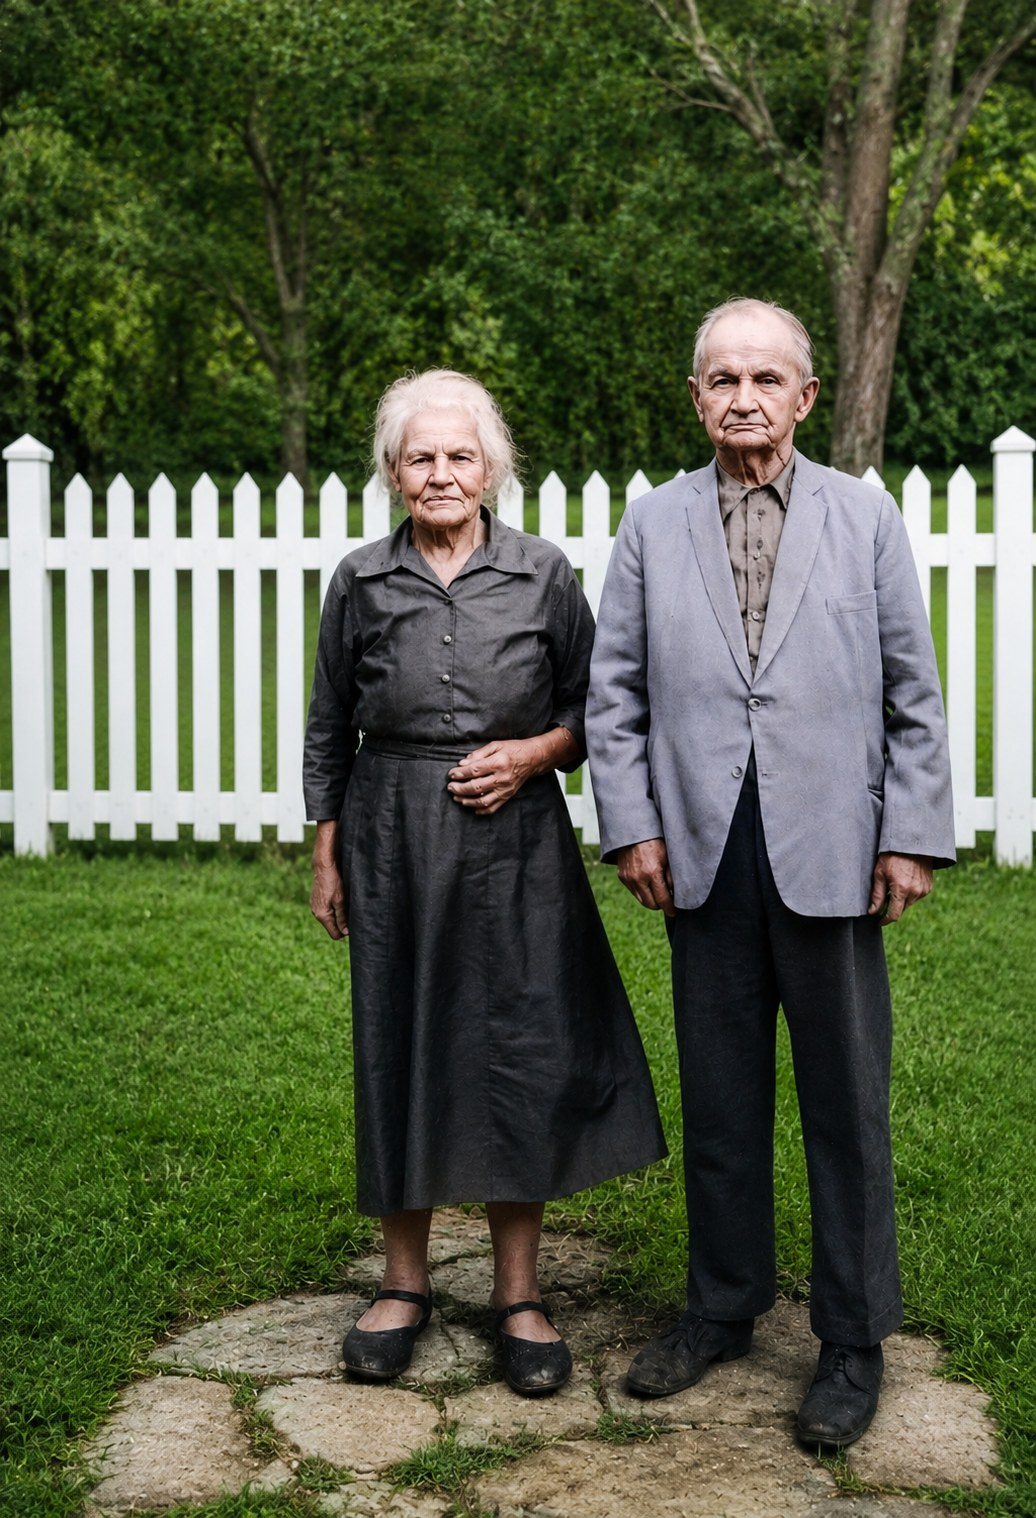
\includegraphics[width=0.7\linewidth,height=\textheight,keepaspectratio,alt={Das letzte gemeinsame Foto des Fata und der Mota, in Aurora. Dies ist eine mit künstlicher Intelligenz überarbeitete Fassung des Originals: Der weiße Zaun, der Rasen, die Bäume und die Farben sind Erfindungen der Maschine, und die Gesichter könnten retuschiert sein. Das verblasste Original ist das Dokument; dies ist eine Illustration davon.}]{imagens/haas_fata_e_mota_aurora_versao_ia.jpg}
\caption{Das letzte gemeinsame Foto des Fata und der Mota, in Aurora.
Dies ist eine mit künstlicher Intelligenz überarbeitete Fassung des
Originals: Der weiße Zaun, der Rasen, die Bäume und die Farben sind
Erfindungen der Maschine, und die Gesichter könnten retuschiert sein.
Das verblasste Original ist das Dokument; dies ist eine Illustration
davon.}
\end{figure}

Johann Haas\index[pessoas]{haas, johann@Haas, Johann} starb am 19. März 1969. Maria Katharina Meier Haas starb am
8. November 1973. Der Text der Familie sagt, beide seien mit 85 Jahren
gestorben. Die genaue Rechnung, die der Meteorologe nicht lassen kann,
ergibt für den \emph{Fata\index[pessoas]{haas, johann@Haas, Johann}} 84 Jahre und acht Monate, knapp vier Monate
vor dem 85. Die \emph{Mota\index[pessoas]{meier, maria@Meier, Maria}} war im April 85 geworden. Der Unterschied
ist für niemanden wichtig, außer für jemanden, der sein Leben lang
Datenreihen korrigiert hat, und ich vermerke ihn nur, damit mir keiner
vorwirft, ich hätte ihn übersehen. Wichtiger ist eine andere Rechnung.
Maria lebte viereinhalb Jahre ohne ihren Mann, in einem Land, dessen
Sprache sie nie sprach, umgeben von Töchtern und Enkeln, die sie durch
die Zuneigung verstanden. 1973 war sie wahrscheinlich einer der letzten
Menschen im Alto Vale, die noch auf Bairisch dachten.

\begin{figure}
\centering
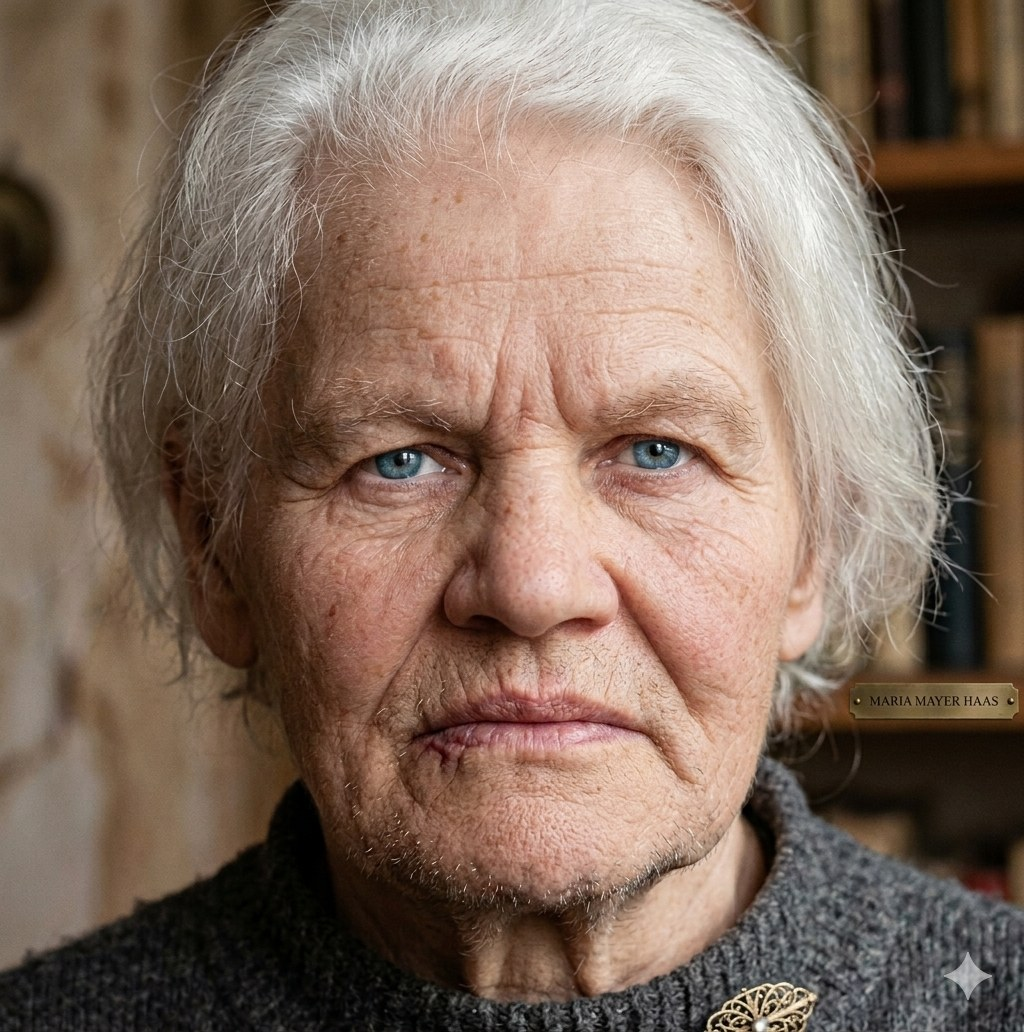
\includegraphics[width=0.55\linewidth,height=\textheight,keepaspectratio,alt={Die Mota im Alter. Mit künstlicher Intelligenz überarbeitete Fassung eines alten Fotos: Das Bücherregal, das Namensschildchen (auf dem die Maschine Mayer schrieb) und die Brosche sind ihre Erfindung, Haut und Haar wurden neu gezeichnet. Die blauen Augen sind die, an die sich die Familie erinnert.}]{imagens/haas_mota_retrato_velhice_versao_ia.jpg}
\caption{Die Mota im Alter. Mit künstlicher Intelligenz überarbeitete
Fassung eines alten Fotos: Das Bücherregal, das Namensschildchen (auf
dem die Maschine \emph{Mayer} schrieb) und die Brosche sind ihre
Erfindung, Haut und Haar wurden neu gezeichnet. Die blauen Augen sind
die, an die sich die Familie erinnert.}
\end{figure}

Ein Foto aus diesen letzten Jahren sagt mehr als die Daten. Die Mota\index[pessoas]{meier, maria@Meier, Maria}
sitzt, mit weißem Haar, geblümtem Kleid und langem Rock, die Hände auf
den Knien. Um sie herum stehen drei Frauen, und die jüngste hält ein
Baby im Arm. Es sind fünf Generationen: die Mota\index[pessoas]{meier, maria@Meier, Maria}, eine Tochter, eine
Enkelin, eine Urenkelin und ein Ururenkel. Das Mädchen aus Heumaden\index[lugares]{heumaden@Heumaden}, das
für Lohn Kühe molk, das 1907 in Schwarz heiratete und mit zwei kleinen
Kindern über den Ozean fuhr, erlebte noch, wie sie die vierte in
Brasilien geborene Generation im Arm halten konnte. Dem Alter nach muss
die Tochter Gertrudes sein, die Älteste, die kurz nach der Ankunft zur
Welt kam. Wer die anderen sind und wer das Baby ist, müssen mir die
Vettern und Cousinen noch sagen.

\begin{figure}
\centering
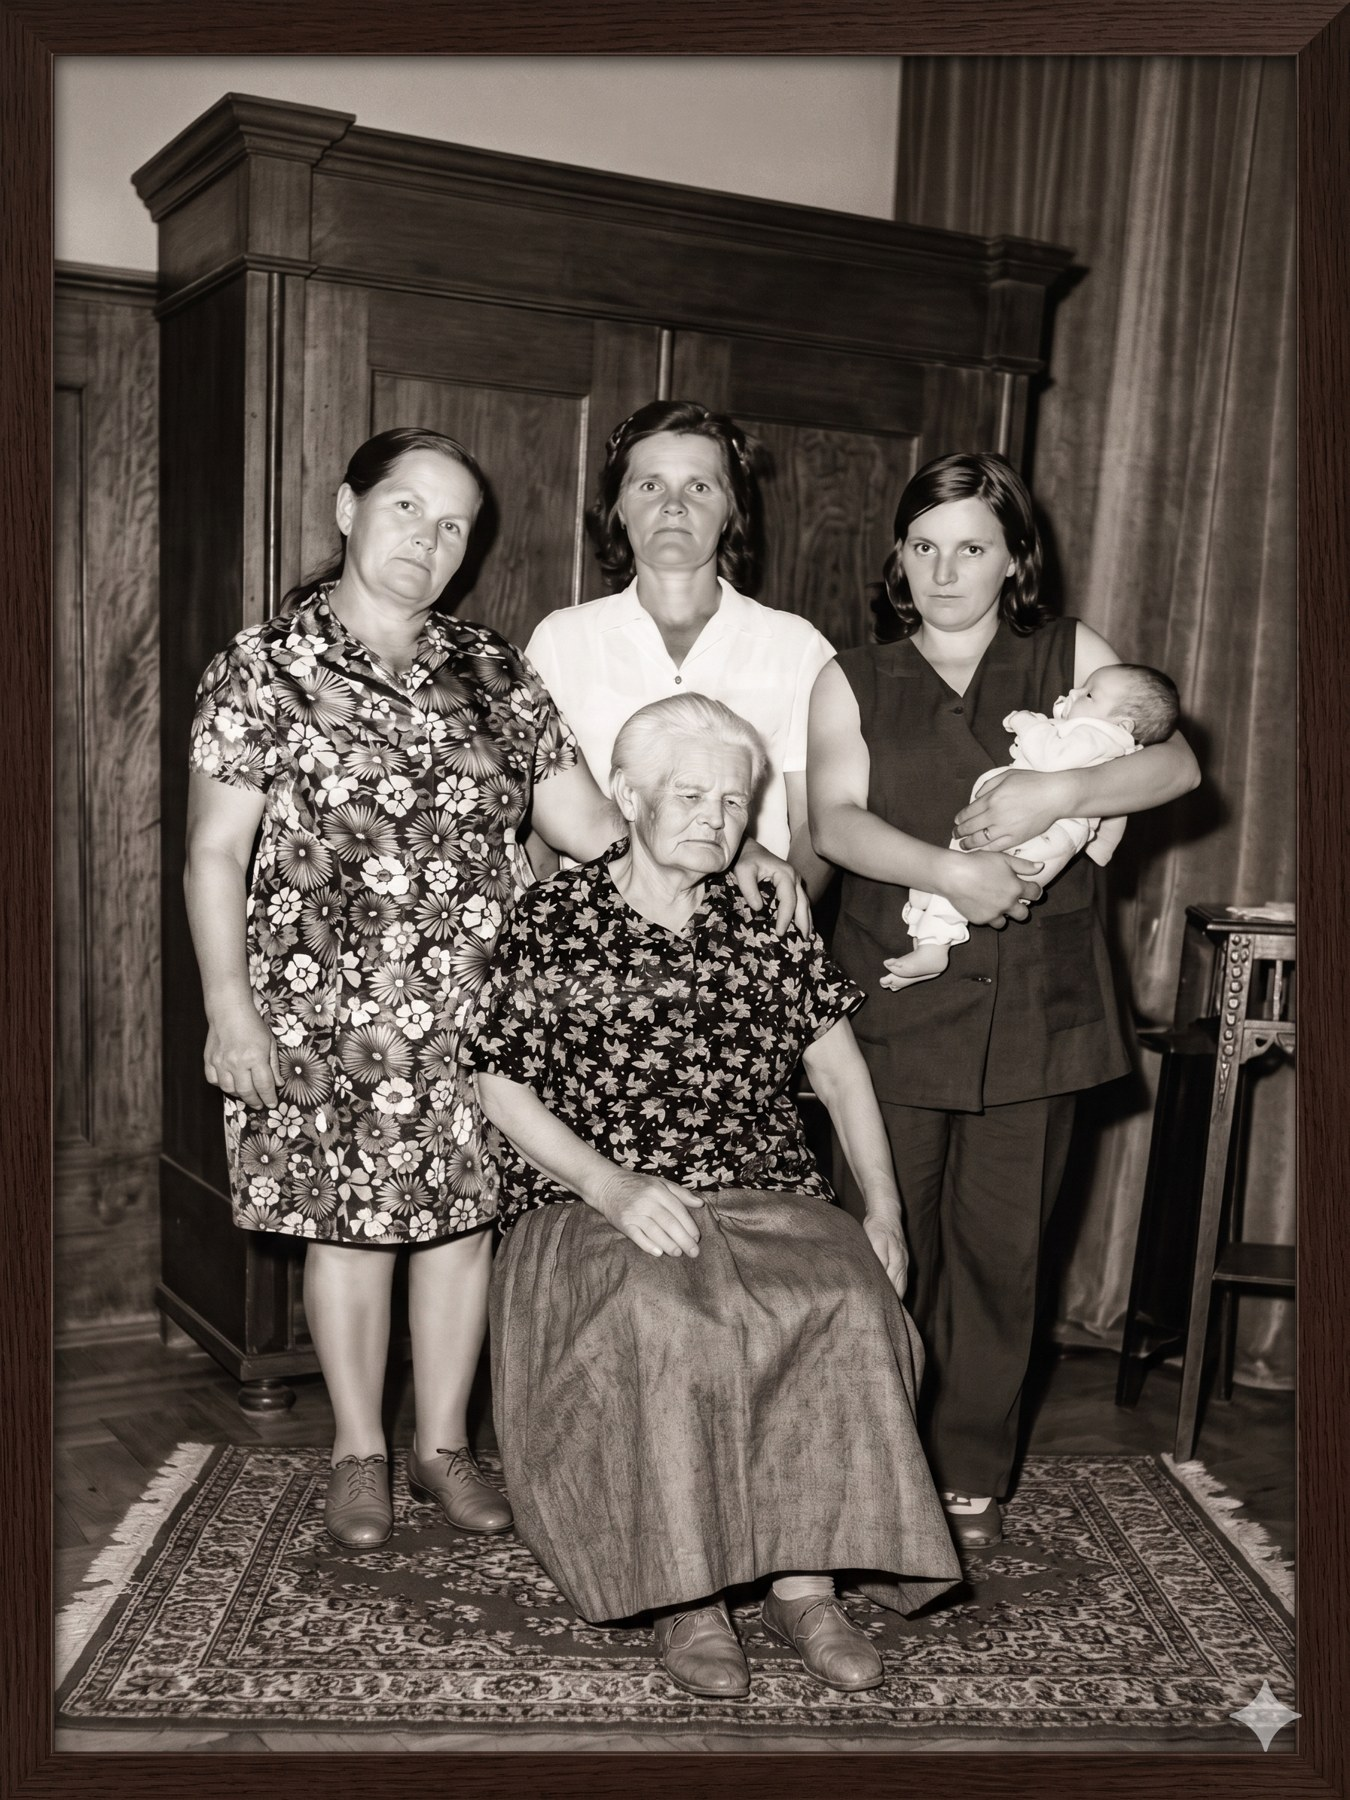
\includegraphics[width=0.7\linewidth,height=\textheight,keepaspectratio,alt={Fünf Generationen: die Mota, sitzend, mit einer Tochter, einer Enkelin und einer Urenkelin, die einen Ururenkel im Arm hält, Anfang der 1970er Jahre. Familienbesitz. Mit künstlicher Intelligenz restaurierte Fassung; Schrank, Vorhang und Teppich könnten von der Maschine neu gemacht sein, und die Namen müssen noch mit der Familie bestätigt werden.}]{imagens/haas_mota_cinco_geracoes_versao_ia.jpg}
\caption{Fünf Generationen: die Mota, sitzend, mit einer Tochter, einer
Enkelin und einer Urenkelin, die einen Ururenkel im Arm hält, Anfang der
1970er Jahre. Familienbesitz. Mit künstlicher Intelligenz restaurierte
Fassung; Schrank, Vorhang und Teppich könnten von der Maschine neu
gemacht sein, und die Namen müssen noch mit der Familie bestätigt
werden.}
\end{figure}

Sie liegen auf dem Friedhof von Aurora\index[lugares]{aurora@Aurora} begraben, neben vielen Gräbern,
die er gemacht hat. Ich schreibe diesen Satz und denke an die Gipsengel
von Rio do Ouro\index[lugares]{rio do ouro@Rio do Ouro}, die ersten, die er formte, um 1914, 1915 das Brot für
die Familie zu kaufen, als der saure Boden von Parzelle 17 nichts
hergab. Ein halbes Jahrhundert später wachen die Engel, die er für die
Toten anderer gemacht hat, über seinen Schlaf. Welche Gräber genau von
ihm sind, sagt der Text der Hundertjahrfeier nicht, und die Frage steht
auf der Liste der offenen Punkte. Dass ihn sein Handwerk bis zum Ende
begleitet hat, muss man aber nicht mehr beweisen.

Das Alto Vale, in dem die beiden ruhen, ist das Tal des Itajaí\index[lugares]{itajai@Itajaí} do Sul
und seiner Zuflüsse, dasselbe, das ich heute mit hydrologischen Modellen
untersuche. Zehn Jahre nach dem Tod der \emph{Mota\index[pessoas]{meier, maria@Meier, Maria}}, im Juli 1983, in
einem Jahr mit einem starken El Niño, fiel tagelang Regen auf das
Einzugsgebiet des Itajaí\index[lugares]{itajai@Itajaí}, und das Wasser stieg in Blumenau\index[lugares]{blumenau@Blumenau} auf etwa 15
Meter. Im August 1984 kam ein weiteres Hochwasser, das in Blumenau\index[lugares]{blumenau@Blumenau} die
Marke des Vorjahres ein wenig übertraf. Rio do Sul\index[lugares]{rio do sul@Rio do Sul}, gleich unterhalb von
Aurora\index[lugares]{aurora@Aurora}, stand beide Male unter Wasser, und das ganze Alto Vale lernte
von Neuem, dass es in einem Flussbecken lebte. Wenn ich auf meinen
Karten die Überschwemmungsflächen von 1983 und 1984 über dem Alto Vale
sehe, denke ich, dass die Familie, wie alle Siedlerfamilien, sich
entschieden hatte, am Wasser zu wohnen. Das Wasser war Weg, Kraft und
Gefahr zugleich. Zu diesen Flüssen kehre ich in Kapitel 13 zurück.

Johann und Maria hatten Bayern\index[lugares]{bayern@Bayern} im März 1913 mit zwei kleinen Kindern
verlassen und, der Überlieferung nach, einem Baby unterwegs. Sie
hinterließen in Brasilien sieben großgezogene Kinder, Dutzende Enkel und
einen Namen, der in die Kirchen von Ituporanga\index[lugares]{ituporanga@Ituporanga} geschrieben ist. Viele
Jahre lang schrieb ich auf eben dieser Seite, sie hätten auch einen
abgeschnittenen Faden hinterlassen: dass seit dem Krieg niemand aus der
Familie mehr nach Deutschland geschrieben habe und dass, als Maria
starb, auf der anderen Seite niemand davon erfuhr. Ich hatte unrecht,
und dieser Irrtum ist die beste Nachricht dieses Kapitels.

\section{Die Briefe aus Rempesgrün}\label{die-briefe-aus-rempesgruxfcn}

\emph{Ribeirão das Pacas\index[lugares]{ribeirao das pacas@Ribeirão das Pacas}, Aurora\index[lugares]{aurora@Aurora}, und Rempesgrün\index[lugares]{rempesgrun@Rempesgrün}, Sachsen\index[lugares]{sachsen@Sachsen}, 1971 bis
1974}

Im November 2026, als dieses Buch schon erschienen war, tauchte in der
Familie ein Bündel Luftpostumschläge auf, aus dünnem Papier, mit
Briefmarken der Deutschen Demokratischen Republik. Einer, mit der
Schreibmaschine adressiert, war an die \emph{Familie Johann Haas\index[pessoas]{haas, johann@Haas, Johann}} im
Alto Vale gerichtet. Die anderen gingen an Onkel Martin\index[pessoas]{sautner, martin@Sautner, Martin} Sautner, den
Mann von Tante Maria, der jüngsten Tochter des Fata\index[pessoas]{haas, johann@Haas, Johann} und der Mota\index[pessoas]{meier, maria@Meier, Maria}, in
Ribeirão das Pacas\index[lugares]{ribeirao das pacas@Ribeirão das Pacas}. Als Absender stand auf der Rückseite Walter Heckel\index[pessoas]{heckel, walter@Heckel, Walter}
aus Rempesgrün\index[lugares]{rempesgrun@Rempesgrün}, einem Dorf bei Auerbach\index[lugares]{auerbach@Auerbach} im sächsischen Vogtland\index[lugares]{vogtland@Vogtland}, drei
Kilometer von Dorfstadt\index[lugares]{dorfstadt@Dorfstadt} und Falkenstein\index[lugares]{falkenstein@Falkenstein} entfernt. Es ist dieselbe
Gegend, aus der die Briefe kamen, die die Familie immer aufbewahrt hat,
und nur ein paar Dutzend Kilometer von Eibenstock\index[lugares]{eibenstock@Eibenstock}, wo Johann und Maria
1907 geheiratet hatten.

Darin lagen vier Briefe. Sie wurden nur zur Hälfte eingescannt, jeweils
das obere linke Viertel des Blattes, und das Ende der Zeilen ist
abgeschnitten. Trotzdem reicht das Lesbare, um die Geschichte zu
verändern.

Der erste ist auf den 22. August 1971 datiert. Die Mota\index[pessoas]{meier, maria@Meier, Maria} lebte noch, sie
war dreiundachtzig. Es schreibt eine Frau, in einer runden Schrift der
alten Schule, mit einem kleinen Bogen über jedem \emph{u}. Dieser Bogen
ist eine Gewohnheit aus der alten deutschen Schreibschrift, der
\emph{Kurrent}, wo er das \emph{u} vom \emph{n} unterschied; sie schrieb
in lateinischer Schrift und konnte die Bewegung aus der Schulzeit doch
nicht ablegen. Sie bedankt sich für den Brief, der am 17. August
angekommen war, bedankt sich dafür, dass man die Freundschaft nicht
abreißen lässt, und schreibt dann die Zeile, bei der ich innehalten
musste:

\emph{Oft d{[}\ldots{]} am Bahnhof das habe ich n{[}\ldots{]} liebe
Schwester nicht mehr sehe.}

Das Ende der Zeilen ging beim Scannen verloren, doch der Sinn lässt
keinen Zweifel: Oft denkt sie an den Bahnhof und hat nie vergessen, dass
sie die liebe Schwester nicht mehr wiedersehen würde. Gleich darunter
erzählt sie, dass sie sich oft mit den beiden anderen Schwestern und mit
Karl\index[pessoas]{meier, karl@Meier, Karl} trifft und dass bei jedem Treffen jemand fragt, ob Post aus
Brasilien gekommen sei, denn sie hätten der Mutter versprochen, einander
weiter zu schreiben.

In Kapitel 4 habe ich mir einen Bahnhof im März 1913 vorgestellt, nach
dem Abschiedsfoto, und ich schrieb dazu, dass ich ihn mir
\emph{vorstellte}. Jetzt weiß ich, dass es einen Bahnsteig gab, dass
eine Schwester der Mota\index[pessoas]{meier, maria@Meier, Maria} darauf stand und sich achtundfünfzig Jahre lang
daran erinnerte.

\begin{figure}
\centering
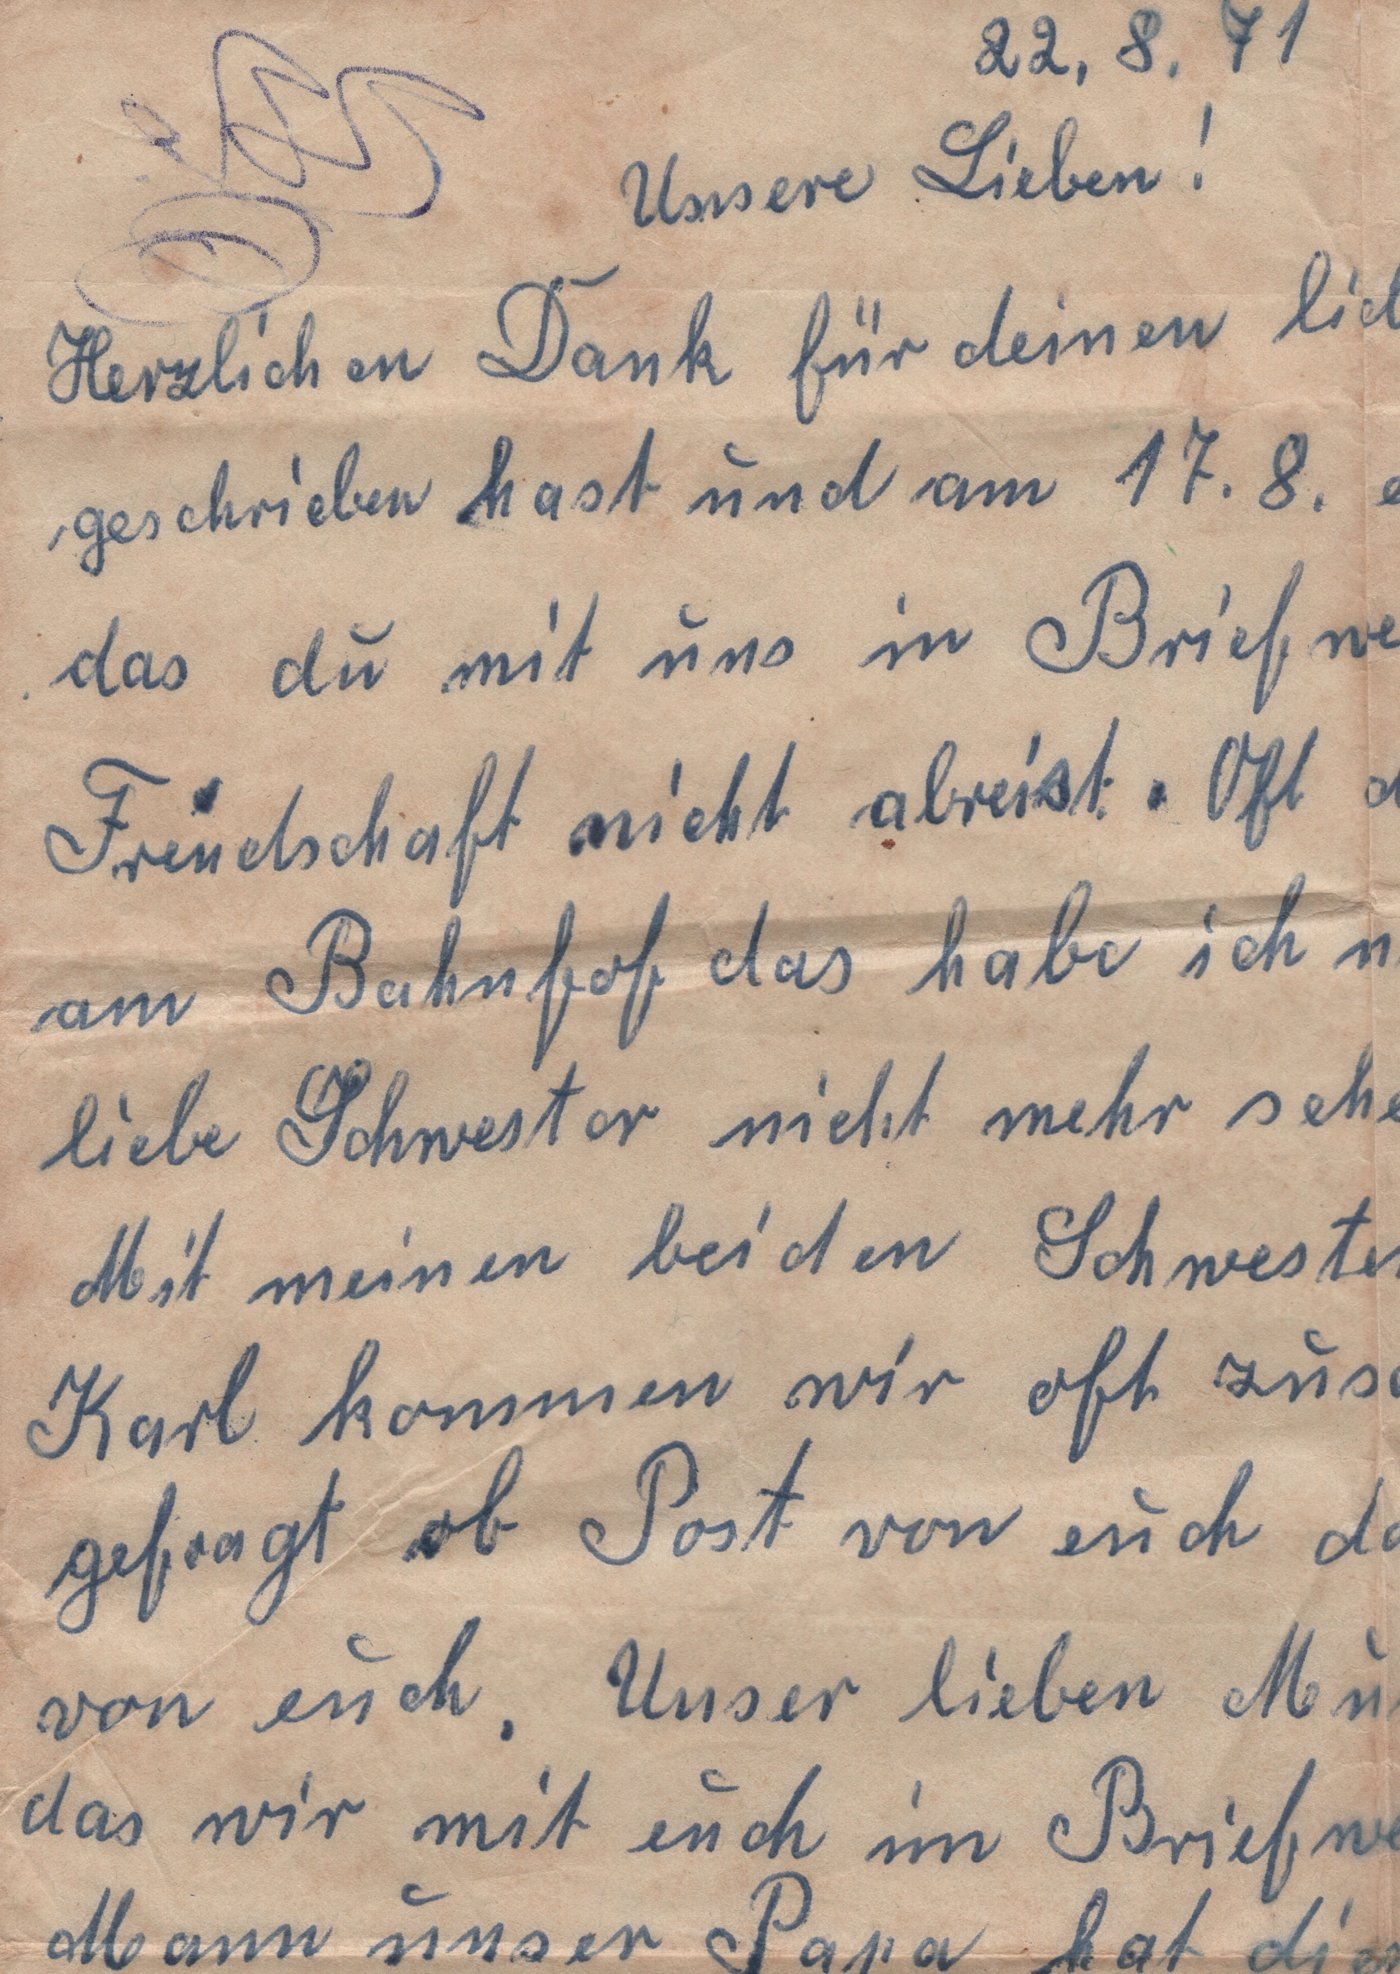
\includegraphics[width=0.75\linewidth,height=\textheight,keepaspectratio,alt={Der Anfang des Briefes vom 22. August 1971, geschrieben in Rempesgrün von einer Schwester der Mota. Achtet auf den kleinen Bogen über jedem u. Die rechte Seite des Blattes liegt außerhalb des Scans.}]{imagens/carta_rempesgruen_1971.jpg}
\caption{Der Anfang des Briefes vom 22. August 1971, geschrieben in
Rempesgrün\index[lugares]{rempesgrun@Rempesgrün} von einer Schwester der Mota\index[pessoas]{meier, maria@Meier, Maria}. Achtet auf den kleinen Bogen
über jedem \emph{u}. Die rechte Seite des Blattes liegt außerhalb des
Scans.}
\end{figure}

Der zweite Brief, ohne sichtbares Datum, beginnt mit
\emph{Rempesg{[}rün{]}} und ist von einer anderen, jüngeren Hand
geschrieben. Darin heißt es, jeder Brief aus Brasilien sei ein
\emph{Freudentag}; es sei bald sechzig Jahre her, dass man sich zuletzt
gesehen habe, was ihn etwa auf 1972 datiert; es sei gut zu wissen, dass
alle sich gut um die Mutter kümmerten und dass sie eine kleine Rente
bekomme. Die Schreiberin fragt nach Namen und Anschrift von jemandem aus
der Familie, der in Westdeutschland sein soll, und erzählt, dass ihr
Sohn Freunde in Veszprém in Ungarn habe und dass Ungarn, wie sie selbst,
sozialistisch sei.

Der dritte ist auf den 3. Januar 197{[}4{]} datiert, die letzte Ziffer
ist abgeschnitten, und er wurde nach dem Tod der Mota\index[pessoas]{meier, maria@Meier, Maria} geschrieben, denn
darin ist von den Eltern die Rede, \emph{die nicht mehr am Leben sind}.
Er beginnt so: \emph{Wir bedauern das Ableben Eurer l{[}ieben{]} Mutter.
Ihr Leben bestand aus M{[}ühe und{]} Sorge. Es bleibt eben niemand auf
{[}dieser{]} Erde.} Dann dankt er Tante Maria für den Brief und die
Fotos und erklärt mit einer Offenheit, über die ich lachen und fast
zugleich weinen musste, dass dort niemand den Brief übersetzen konnte,
weil er auf Portugiesisch geschrieben war, und die Sprachen dort
Deutsch, Englisch und Russisch seien. Onkel Martin\index[pessoas]{sautner, martin@Sautner, Martin}, heißt es, habe ihnen
immer schöne Briefe auf Deutsch geschrieben. Und er bittet darum, dass
der Briefwechsel nicht aufhört, auch wenn die Eltern nicht mehr leben:
Man brauche keine langen Briefe zu schreiben, Hauptsache, man wisse
immer, was auf dieser Seite vor sich gehe.

Der vierte ist wieder von der Frau mit dem Bogen über dem \emph{u}. Er
hat kein sichtbares Datum. Sie schreibt, sie habe lange auf Nachricht
gewartet und müsse mitteilen, dass Walter, ihr Mann, gestorben ist. Er
war blind und konnte nicht mehr gehen. Sein letztes Wort, schreibt sie,
sei ihr Name gewesen, so jedenfalls lese ich die abgeschnittene Zeile.
\emph{Es geht ein nach den andern.} Dann erzählt sie von den Söhnen,
Hans und Horst, von einem schönen Haus, das sie nach und nach
verschönern, und dass sie drei Schafe hat.

Die Schwester unserer Mota\index[pessoas]{meier, maria@Meier, Maria} war also die Frau von Walter Heckel\index[pessoas]{heckel, walter@Heckel, Walter}, und sie
war es, die aus Rempesgrün\index[lugares]{rempesgrun@Rempesgrün} schrieb. Für mich ist sie Theresia\index[pessoas]{meier, theresia@Meier, Theresia} Meier, die
kleine Schwester, die am 22. Juni 1891 geboren wurde, als die Mota\index[pessoas]{meier, maria@Meier, Maria} drei
Jahre alt war, und die dieselbe Patin hatte wie sie. Die Unterschrift,
die den Namen bestätigen würde, blieb in der Hälfte des Blattes, die der
Scanner nicht erfasst hat, und eines Tages werdet ihr sie lesen können.

Wer den Faden jahrzehntelang hielt, war Onkel Martin\index[pessoas]{sautner, martin@Sautner, Martin} Sautner. Die Mota\index[pessoas]{meier, maria@Meier, Maria}
schrieb nicht auf Portugiesisch, die Töchter und Enkel schrieben nicht
mehr auf Deutsch, und er war es, der sich in Ribeirão das Pacas\index[lugares]{ribeirao das pacas@Ribeirão das Pacas} an den
Tisch setzte und auf Deutsch auf die andere Seite des Eisernen Vorhangs
schrieb. Als die Mota\index[pessoas]{meier, maria@Meier, Maria} starb, erfuhr die Familie drüben davon. Sie
schickte ihr Beileid. Sie bat darum, nicht aufzuhören.

Und wir hörten auf. Ich weiß nicht, wann der letzte Brief kam und wer
nicht mehr antwortete. Ich weiß, dass mir, als ich 2012 mit dieser
Recherche begann, niemand von den Verwandten in Rempesgrün\index[lugares]{rempesgrun@Rempesgrün} erzählte und
dass ich Verwandte in Bayern\index[lugares]{bayern@Bayern} suchte, wo sie nicht waren. Die Karte hatte
ein Loch, aber es war nicht das Loch des Krieges: Es war unseres. Bevor
ich versuchen konnte, es zu schließen, musste ich noch viel weiter
zurückgehen. Meine Mutter, Adelina Doerner\index[pessoas]{doerner, adelina@Doerner, Adelina}, stammte von Leuten ab, die
fünfundachtzig Jahre vor der \emph{Formosa} nach Santa Catarina gekommen
waren, auf Segelschiffen, in einer Zeit, in der es noch keinen Dampf und
keine Quarantäne von Hafen zu Hafen gab, wohl aber die Flaute. Die
nächste Station dieser Rückwärtstrajektorie liegt in der Bucht von
Desterro\index[lugares]{desterro@Desterro}, im November 1828.

\section{Für euch zum Entdecken}\label{fuxfcr-euch-zum-entdecken-6}

\begin{itemize}
\tightlist
\item
  Wer sind, mit Namen, die fünf Generationen auf dem Foto mit der Mota\index[pessoas]{meier, maria@Meier, Maria},
  und wo und wann wurde es aufgenommen?
\item
  Welcher Enkel stand an der Straße Wache, während unten im Keller das
  Radio lief? Fragt die älteren Cousins und Cousinen.
\item
  Was wollte der Fata\index[pessoas]{haas, johann@Haas, Johann} 1939: einen Besuch oder die endgültige Rückkehr?
  War eine Fahrkarte gekauft oder nur ein Wunsch bei Tisch
  ausgesprochen? Wer die Fassungen von damals gehört hat, erinnert sich
  vielleicht noch an eine davon.
\item
  Auf welchem Weg gingen die Kisten von 1945, und kam je eine Antwort
  aus Deutschland zurück?
\item
  Welche Gräber auf dem Friedhof von Aurora\index[lugares]{aurora@Aurora} hat der Fata\index[pessoas]{haas, johann@Haas, Johann} gemacht? Der
  Text der Hundertjahrfeier sagt es nicht. Geht hin und schaut nach, und
  fragt die Enkel aus Aurora\index[lugares]{aurora@Aurora}.
\item
  Bestätigt die Unterschrift der Briefe, dass Tante Theresia\index[pessoas]{meier, theresia@Meier, Theresia} sie
  geschrieben hat? Und wer waren die beiden anderen Schwestern und der
  Bruder Karl\index[pessoas]{meier, karl@Meier, Karl}? Die vollständigen Blätter der Briefe, in A4 eingescannt,
  Vorder- und Rückseite, müssten die Antwort tragen.
\item
  Wer aus der Familie war um 1972 in Westdeutschland, die Person, nach
  deren Adresse die Verwandten in Rempesgrün\index[lugares]{rempesgrun@Rempesgrün} fragten?
\item
  Wo sind die Briefe, die Onkel Martin\index[pessoas]{sautner, martin@Sautner, Martin} geschrieben hat? Wenn die
  Verwandten drüben sie so aufbewahrt haben wie wir ihre, erzählen sie
  unsere Seite der Geschichte.
\end{itemize}

\part{Die Pioniere von 1828, die Mosel und die Klingen von
Solingen\index[lugares]{solingen@Solingen}}\label{die-pioniere-von-1828-die-mosel-und-die-klingen-von-solingen}

\begin{boletim}

Nordostpassat. Segelschiffe in der äquatorialen Flaute festgehalten.
Sichtweite: fast zwei Jahrhunderte.

\end{boletim}

\chapter{12. November 1828 --- Die ersten Schiffe von
Desterro\index[lugares]{desterro@Desterro}}\label{cap-8}

\begin{quote}
\emph{Vor der Dampfschifffahrt bestimmte der Wind den Tag der Ankunft.}
\end{quote}

\emph{49,7° N · 6,9° O, Hermeskeil\index[lugares]{hermeskeil@Hermeskeil}, Hunsrück\index[lugares]{hunsruck@Hunsrück} · 27,6° S · 48,8° W, São
Pedro de Alcântara, SC}

Ich weiß nicht, auf welchem Schiff Anton Michels\index[pessoas]{michels, anton@Michels, Anton} den Ozean überquerte.
Die Notiz, die ich über ihn habe, nennt zwei Routen mit zwei
Ankunftsdaten in Desterro\index[lugares]{desterro@Desterro}, fünf Tage auseinander. Ignazia Loch\index[pessoas]{loch, ignazia@Loch, Ignazia}, aus
demselben Zweig, hat einen Geburtseintrag an einem Ort, den es im
angegebenen Jahr noch gar nicht gab. Bernard Preis\index[pessoas]{preis, bernard@Preis, Bernard} hat ein Geburtsjahr
auf dem Papier und ein anderes auf dem Grabstein.

Bis hierher bin ich der Seite meines Vaters gefolgt, der näheren und
besser belegten Seite. Die Haas kamen 1913, und es gab Enkel, die noch
die Stimme des \emph{Fata\index[pessoas]{haas, johann@Haas, Johann}} Geschichten erzählen hörten. Wenn ich zur
Seite meiner Mutter, Adelina Doerner\index[pessoas]{doerner, adelina@Doerner, Adelina}, wechsle, ändert sich der
Zeitmaßstab. Die Michels, die Arns und, wie es scheint, die Preiss und
die Loch kamen nicht mit einem Dampfer nach Santa Catarina, mit
maschinengeschriebener Passagierliste und Hafenstempel. Sie kamen auf
Segelschiffen, fast ein Jahrhundert früher (die Doerner sollten später
kommen, auf einem anderen Weg), als Brasilien noch einen Kaiser hatte,
die Insel Santa Catarina Desterro\index[lugares]{desterro@Desterro} hieß und es in der Provinz keine
einzige deutsche Kolonie gab.

Der mütterliche Zweig ist deshalb aus anderem Stoff gemacht. Auf der
Haas-Seite hatte ich Erinnerung und suchte Dokumente. Auf der
Doerner-Seite habe ich Dokumente, viele, verstreut über
Kirchenbuchregister, Schiffslisten und Notizen deutscher und
brasilianischer Genealogen, und fast keine Erinnerung. Niemand hat Anton
Michels an Land gehen sehen. Niemand hat seine Stimme bewahrt. Was ich
habe, sind Daten, manche sicher, andere unmöglich, und Schreibweisen,
die sich mit jedem Schreiber ändern. Dieses Kapitel ist ein Versuch,
diesem Skelett Fleisch zu geben, ohne so zu tun, als wäre es mehr, als
es ist.

\section{Hermeskeil, Sommer 1828}\label{hermeskeil-sommer-1828}

\emph{Hermeskeil\index[lugares]{hermeskeil@Hermeskeil}, Hochwald im Hunsrück\index[lugares]{hunsruck@Hunsrück}, Rheinprovinz (Preußen), Juni
1828}

Anton Michels\index[pessoas]{michels, anton@Michels, Anton} wurde am 11. Mai 1822 in Hermeskeil\index[lugares]{hermeskeil@Hermeskeil} geboren und am
folgenden Tag getauft. Hermeskeil\index[lugares]{hermeskeil@Hermeskeil} liegt im Hochwald, dem hohen,
bewaldeten Teil des Hunsrücks, etwa dreißig Kilometer südöstlich von
Trier. Für einen Meteorologen ist das ein Ort, den man sich leicht
vorstellen kann: eine Hochfläche mittlerer Höhe, den Westwinden
ausgesetzt, die feucht vom Atlantik kommen und ihre Last als
Nieselregen, Nebel und lange Winter abladen. Ein Land für Roggen, Hafer,
Kartoffeln und Wald, weniger für Weizen. Ein Land, von dem man leben
konnte, wenn jede Familie genug davon hatte.

Die Familien hatten nicht genug. Um zu verstehen, warum ein
sechsjähriger Junge in Bremen die Planke eines Schiffes hinaufsteigt,
muss man eine Rechtsregel verstehen, die keiner meiner Vorfahren je
gelesen, die aber jeder von ihnen zu spüren bekommen hat: die
\emph{Realteilung}. Im Hunsrück\index[lugares]{hunsruck@Hunsrück}, an der Mosel\index[lugares]{mosel@Mosel}, in weiten Teilen des
Rheinlands und der Pfalz wurde das Land eines Vaters bei seinem Tod zu
gleichen Teilen unter allen Kindern aufgeteilt. Das klingt gerecht, und
in gewissem Sinn ist es das auch, nur wurden die Felder mit jeder
Generation von Neuem geteilt. Aus einem Acker, der eine Familie
ernährte, wurden zwei Streifen, die zwei Familien halb ernährten, dann
vier Streifen, die niemanden ernährten. Anfang des 19. Jahrhunderts gab
es Dörfer im Hunsrück\index[lugares]{hunsruck@Hunsrück}, in denen ein Bauer zehn oder fünfzehn Flurstücke
bewirtschaftete, über die ganze Gemarkung verstreut, jedes so groß wie
ein Hof. Im altbayerischen Land der Haas galt das Gegenteil, das
Anerbenrecht, und die Geschwister, die nicht erbten, wurden Ziegler und
Fabrikarbeiter. Hier erbten alle, und alle erbten wenig. Zwei
entgegengesetzte Wege zum selben Ergebnis: zu viele Menschen auf dem
Land.

Dazu kam das Klima, und hier bittet der Meteorologe ums Wort. Im April
1815 hatte der Vulkan Tambora in Indonesien einen der größten Ausbrüche
der letzten Jahrtausende. Der Schleier aus Schwefelaerosolen, der in die
Stratosphäre aufstieg, breitete sich über den Planeten aus und warf
einen Teil des Sonnenlichts zurück. Das folgende Jahr, 1816, ging in
Europa als das Jahr ohne Sommer in die Erinnerung ein: Frost im Juni,
endloser Regen, Ernten, die auf dem Feld verfaulten. Im Rheinland und im
Südwesten Deutschlands waren 1816 und 1817 Hungerjahre. Anton war noch
nicht geboren, aber er kam in einer Gegend zur Welt, die sich an diesen
Hunger erinnerte und daraus gelernt hatte, dass das Land versagen
konnte. Außerdem war das Rheinland nach dem Wiener Kongress gerade an
Preußen gefallen, mit neuen Steuern, Militärdienst und einer fernen
Verwaltung.

Auf diesen Boden fielen die Versprechungen der Auswanderungsagenten. In
den 1820er Jahren wollte das gerade unabhängig gewordene Kaiserreich
Brasilien europäische Siedler, um den Süden zu besetzen und zu
verteidigen, und ließ in Deutschland anwerben. Die Werber sprachen von
kostenlosem Land, von Werkzeug, von Saatgut, von Unterstützung in den
ersten Jahren. Ich stelle mir vor, dass diese Worte im Winter 1827 auf
1828 von Haus zu Haus durch die Dörfer des Hochwalds gingen. Ich stelle
mir auch die Entscheidung von Antons Eltern vor. Ihre Namen konnte ich
in meinen Quellen nicht sicher feststellen, und sie erscheinen hier nur
als „die Eltern``. Sie verkaufen das Wenige, das sie haben, und brechen
im Sommer 1828 mit den Kindern nach Bremen auf, um über den Ozean zu
fahren.

Für einen Sechsjährigen muss schon die Reise bis zum Hafen das größte
Abenteuer seines Lebens gewesen sein. Erst die Wege des Hunsrücks, dann
die Flüsse, dann die norddeutsche Tiefebene, die er nie gesehen hatte,
ohne Hügel und ohne Wald, mit einem riesigen Himmel. Bremen, die Masten,
der Geruch nach Teer. Wahrscheinlich verstand er das Wort
\emph{Brasilien} nicht. Er verstand, dass er mit der Familie irgendwohin
fuhr, und für ein Kind genügt das.

\section{Zwei Routen für denselben
November}\label{zwei-routen-fuxfcr-denselben-november}

\emph{Bremen, Juni und Juli 1828}

Der erste Zweifel taucht schon am Kai auf. Das Profil von Anton Michels\index[pessoas]{michels, anton@Michels, Anton}
bei FamilySearch enthält in den Notizen eine Zusammenfassung aus
deutschen Quellen, die ich hier wiedergebe, weil sie die beste
Beschreibung der Reise ist, die ich habe, und weil sie offen zeigt, dass
man nicht weiß, auf welchem Schiff er kam.

\begin{ficha}

\textbf{Archivkarte}: Notiz im Profil von Anton Michels\index[pessoas]{michels, anton@Michels, Anton} bei FamilySearch
(LDL7-7XZ), auf Deutsch, mit Verweis auf die Zusammenstellung
\emph{Emigration nach Brasilien 1828} von Ursula Buchholz. Sinngemäß:
„Am 7. November 1828 kamen mit der \emph{Luiza} 276 Personen in der
Kolonie São Pedro de Alcântara\index[lugares]{sao pedro de alcantara@São Pedro de Alcântara} an. Am 12. November 1828 kamen mit der
\emph{Marquês de Viana} weitere 259 Personen. Von diesen kamen 523
Kolonisten direkt aus Bremen (Bremerhaven). Darunter Leute aus den
Kreisen Cochem, Mayen, Bernkastel-Wittlich und Trier-Saarburg.`` Es
folgen zwei mögliche Routen: ab Bremen am 28. Juni 1828 mit der
\emph{Johanna Jakobs} nach Rio de Janeiro\index[lugares]{rio de janeiro@Rio de Janeiro} und von dort im Oktober mit
der \emph{Luiza} nach Desterro\index[lugares]{desterro@Desterro} (Ankunft am 7. November); oder ab Bremen
am 6. Juli 1828 mit der \emph{Charlotte \& Louise} nach Rio und von dort
im Oktober mit der \emph{Marquês de Viana} nach Desterro\index[lugares]{desterro@Desterro} (Ankunft am 12.
November). Als Einwanderungsdatum ist für Anton der 12. November 1828
eingetragen.

\end{ficha}

Die Notiz sagt „oder``. Das Datum, das in Antons Eintrag steht, der 12.
November, ist das der Ankunft der \emph{Marquês de Viana}, und danach
wäre er in Bremen auf der \emph{Charlotte \& Louise} abgefahren. Aber
dieselbe Notiz bietet die andere Route an, die \emph{Johanna Jakobs} und
die \emph{Luiza}, mit Ankunft fünf Tage früher, und genau diese Fassung
kam zuerst in meine Aufzeichnungen und in den Entwurf dieses Buches. Ich
kann es nicht entscheiden. Dazu müsste ich die Passagierlisten mit
seinem Namen sehen, und die habe ich nicht gesehen. Ich bleibe beim 12.
November, dem eingetragenen Datum, halte aber die andere Route am Leben.
In der Genealogie wie in der Wettervorhersage ist es besser, die
Unsicherheit zu veröffentlichen als eine falsche Gewissheit.

In diesen Zahlen steckt noch ein Detail. Von den 535, die mit den beiden
Briggs ankamen, kamen 523 direkt aus Bremen; die übrigen, stelle ich mir
vor, stießen unterwegs dazu, in Rio de Janeiro\index[lugares]{rio de janeiro@Rio de Janeiro}. Und die genannten
Herkunftsgebiete, Cochem, Mayen, Bernkastel-Wittlich und Trier-Saarburg,
zeichnen auf der Karte ein einziges Gebiet: Mosel\index[lugares]{mosel@Mosel} und Hunsrück\index[lugares]{hunsruck@Hunsrück}, das
linke Rheinufer. Die Pioniere von São Pedro de Alcântara\index[lugares]{sao pedro de alcantara@São Pedro de Alcântara} waren zum
großen Teil Nachbarn. Sie kamen aus denselben Hügeln, sprachen denselben
Dialekt und waren vor derselben Erbteilung geflohen. Belegt ist zum
Beispiel eine Familie Berens aus Wintrich an der Mosel\index[lugares]{mosel@Mosel}, die am 7.
November 1828 mit der Brigg \emph{Luiza} ankam und sich in der neuen
Kolonie niederließ.\footnote{Die Familie Berens (Berns) aus Wintrich,
  Bernkastel-Wittlich, wird von Toni Jochem als mit der Brigg
  \emph{Luisa\index[pessoas]{haas, luisa@Haas, Luisa}} am 7. November 1828 angekommen und in São Pedro de
  Alcântara angesiedelt genannt. Siehe den Artikel von Toni Jochem und
  Mitarbeitern über die Kolonien Piedade und Santa Isabel\index[lugares]{santa isabel@Santa Isabel} in der Reihe
  \emph{Páginas da Colonização: Estudos/subsídios históricos sobre a
  Colônia Alemã Santa Isabel\index[lugares]{santa isabel@Santa Isabel} --- 175 anos de Fundação} (2022--2023).}

\section{Flaute}\label{flaute}

\emph{Atlantik, zwischen Ärmelkanal und Rio de Janeiro\index[lugares]{rio de janeiro@Rio de Janeiro}, Juli bis
September 1828}

Ich weiß nicht, wie lange Antons Überfahrt dauerte, aber ich weiß, wie
diese Reisen waren, und ich weiß, wie der Ozean war, den er überquerte,
denn es ist derselbe wie heute. Ein Segelschiff, das Anfang Juli von
Bremen auslief, fuhr die Nordsee hinunter, passierte den Kanal, gewann
den Atlantik und suchte den Nordostpassat, der es mit der Regelmäßigkeit
eines Uhrwerks nach Süden und Südwesten schob. Bis dahin kam die Reise,
mit Glück, voran.

Dann kam der Gürtel, den die Seeleute fürchteten und den ich meinen
Studenten unter einem anderen Namen beibringe. In der Nähe des Äquators
treffen die Passate beider Hemisphären aufeinander, die Luft steigt auf,
bildet hohe Wolken und Schauer, und an der Oberfläche verschwindet der
Wind einfach. Heute nennen wir diesen Gürtel die Innertropische
Konvergenzzone. Die englischen Seeleute nannten ihn \emph{doldrums}, die
portugiesischen \emph{calmarias}, Kalmen. Ein Schiff konnte dort
tagelang liegen bleiben, manchmal wochenlang, mit schlaff hängenden
Segeln, unter einer feuchten Hitze, die nicht nachlässt, und auf einen
Hauch warten, der es von der Stelle brachte. Das Trinkwasser verdarb in
den Fässern, das Essen verdarb, die Kinder wurden krank. An diesem Punkt
der Reise begreift man, dass vor der Dampfschifffahrt der Wind den Tag
der Ankunft bestimmte.

Ich stelle mir Anton vor, sechs Jahre alt, an Deck eines Schiffes, das
mitten im Ozean stillliegt. Vielleicht fand er das schön, das Wasser
glatt wie ein Spiegel und rundherum der Horizont. Vielleicht sah er eine
Seebestattung, denn auf fast jeder Überfahrt jener Zeit starb jemand,
und fast immer waren es die Kinder und die Alten. Ich weiß nicht, ob
seine Familie jemanden verlor. Ich weiß, dass er überlebte. Auf einem
Auswandererschiff von 1828 war es ein Ereignis, dass ein Sechsjähriger
überlebte.

Nach der Flaute trug der Südostpassat das Schiff an der brasilianischen
Küste entlang bis Rio de Janeiro\index[lugares]{rio de janeiro@Rio de Janeiro}. Dort warteten die Kolonisten, gingen
an Land, wurden gezählt und neu verteilt. Im Oktober 1828 schifften sich
die für Santa Catarina Bestimmten auf zwei Küstenbriggs ein, der
\emph{Luiza} und der \emph{Marquês de Viana}, für die letzte Etappe der
Reise nach Süden, entlang einer Küste grüner Bergketten, die keiner von
ihnen kannte.

\section{Ein azorianisches Städtchen und eine Straße nach
Lages}\label{ein-azorianisches-stuxe4dtchen-und-eine-strauxdfe-nach-lages}

\emph{Nossa Senhora do Desterro\index[lugares]{desterro@Desterro}, November 1828 bis März 1829}

Die Brigg lief an einem Novembermorgen in die Bucht von Desterro\index[lugares]{desterro@Desterro} ein.
Wenn es tatsächlich die \emph{Marquês de Viana} war, dann am 12.
November 1828. Dieses Datum gibt dem Kapitel seinen Titel, und ich mag
es auch wegen seiner Unsicherheit, wie eine Beobachtung, die um fünf
Tage danebenliegen kann.

Für einen Jungen aus dem Hunsrück\index[lugares]{hunsruck@Hunsrück} muss das ein anderer Planet gewesen
sein. Die bewaldete Insel, das warme Wasser der Bucht, die weißen Häuser
eines Städtchens von Fischern und Bauern azorianischer Herkunft, die
eine Sprache sprachen, die er nicht verstand, und denselben Glauben
hatten wie er, auch wenn sie anders beteten. Die Bewohner von Desterro\index[lugares]{desterro@Desterro}
wussten ihrerseits nicht, was sie mit diesen Leuten mit hellem Haar und
Wollkleidung anfangen sollten. Ein Ort, der an Maniokmehl und Fisch
gewöhnt war, musste auf einen Schlag mehr als fünfhundert deutsche
Kolonisten unterbringen und ernähren, während die Regierung entschied,
wohin mit ihnen.

Etwas kann der Meteorologe nicht durchgehen lassen. Der Entwurf dieses
Buches sprach in einer ersten Fassung vom „Winter des Wartens`` in
Desterro\index[lugares]{desterro@Desterro}. Das war ein Irrtum der Hemisphäre. Anton kam im November an,
am Ende des südlichen Frühlings, und verbrachte in Desterro\index[lugares]{desterro@Desterro} den Sommer,
den ersten Sommer seines Lebens, in dem der Dezember heiß war. Die
Familie, die Bremen im nördlichen Sommer verlassen hatte, reihte zwei
Sommer aneinander und übersprang einen ganzen Winter. Ich denke gern,
dass der Junge sich über Weihnachten in der Hitze und die langen
Januartage wunderte und dass er irgendwann in jenem Sommer das Wort
\emph{mar}, Meer, auf Portugiesisch lernte.

Das Warten dauerte einige Monate. Im März 1829 wurden die Kolonisten
aufs Festland gebracht und zogen bergwärts, entlang der Straße, die die
Regierung anlegen ließ, um Desterro\index[lugares]{desterro@Desterro} mit Lages auf der Hochebene zu
verbinden. Dort, etwa dreißig Kilometer von der Küste, wurde die Kolonie
São Pedro de Alcântara\index[lugares]{sao pedro de alcantara@São Pedro de Alcântara} gegründet, die erste deutsche Kolonie in Santa
Catarina. Der Gedanke war, die Straße zu besiedeln, damit die Tropeiros,
die Viehtreiber, und ihre Herden unterwegs Unterkunft, Essen und
Menschen fanden, und zugleich Land zu besetzen, das das Kaiserreich für
leer hielt.

Leer war es nicht, aber das ist ein Gespräch, das schon in Kapitel 6
begonnen hat und hier nicht wiederholt werden soll. Gut war es auch bei
Weitem nicht. Die Hänge von São Pedro de Alcântara\index[lugares]{sao pedro de alcantara@São Pedro de Alcântara} waren steil, der
Boden arm und vom Regen ausgewaschen, und die Versprechungen von
Unterstützung und Werkzeug wurden, wie es fünfundachtzig Jahre später
den Haas in Rio do Ouro\index[lugares]{rio do ouro@Rio do Ouro} ergehen sollte, nur zur Hälfte oder gar nicht
eingelöst. In den folgenden Jahren verließen viele Familien die Kolonie
und verteilten sich in die Nachbartäler, nach Santo Amaro, in die
Niederung, wohin auch immer es Land gab, das etwas hergab. Anton Michels\index[pessoas]{michels, anton@Michels, Anton}
folgte dieser Bewegung. Als wir ihn in den Registern wiederfinden, schon
als Mann, lebt er in der Colônia Santa Isabel\index[lugares]{santa isabel@Santa Isabel}, die 1847 weiter oben an
derselben Straße nach Lages gegründet wurde. Er starb 1874 in Vargem
Grande, heute Gemeinde Águas Mornas\index[lugares]{aguas mornas@Águas Mornas}. Zwischen dem Jungen auf der Brigg
und dem Kolonisten von Santa Isabel\index[lugares]{santa isabel@Santa Isabel} liegen fast zwanzig Jahre, von denen
ich nichts weiß. Das nächste Kapitel beginnt, als sein Leben das einer
jungen Frau von der Mosel\index[lugares]{mosel@Mosel} kreuzt.

\section{Ignazia, das Mädchen ohne
Datum}\label{ignazia-das-muxe4dchen-ohne-datum}

\emph{São Pedro de Alcântara\index[lugares]{sao pedro de alcantara@São Pedro de Alcântara}, 1828?}

Im selben Zweig des Stammbaums, zwei Generationen über Gertrudes Preiss\index[pessoas]{preiss, gertrudes@Preiss, Gertrudes},
meiner Großmutter mütterlicherseits, steht ein Paar, das ebenfalls zu
dieser ersten Welle gehört, oder jedenfalls gehören müsste. Es sind
Bernard Preis\index[pessoas]{preis, bernard@Preis, Bernard} und Ignazia Loch\index[pessoas]{loch, ignazia@Loch, Ignazia}, die Eltern von Emanuel Preis\index[pessoas]{preis, emanuel@Preis, Emanuel}, meinem
Urgroßvater, den die Volkszählung von 1920 Manoel Preuss nennen wird.
Über Ignazia sagt der Eintrag Folgendes.

\begin{ficha}

\textbf{Archivkarte}: Profil von Agnes Ignacia (Ignazia) Loch bei
FamilySearch (LV7G-Z2H). Geburt: „1828, São Pedro de Alcântara\index[lugares]{sao pedro de alcantara@São Pedro de Alcântara}, Santa
Catarina, Brasil``. Tod: „von 1872 zu 1914``, also ein geschätzter
Zeitraum ohne Datum. In den Kirchenbuch- und Standesamtsregistern von
Santa Catarina, in denen sie als Mutter oder Großmutter vorkommt, wird
ihr Name geschrieben als Ignacia Loch, Ignazia Locho, Ignacia Lock,
Ignacia Locks, Ignazia Luch, Ignacia Roch und sogar Ignácio Lach.

\end{ficha}

Dieser Eintrag hat ein Problem, das man beim ersten Lesen sieht. Ignazia
kann nicht 1828 in São Pedro de Alcântara\index[lugares]{sao pedro de alcantara@São Pedro de Alcântara} geboren sein, denn 1828 gab es
São Pedro de Alcântara\index[lugares]{sao pedro de alcantara@São Pedro de Alcântara} nicht. Die Kolonisten kamen im November jenes
Jahres in Desterro\index[lugares]{desterro@Desterro} an, und die Kolonie wurde erst im März 1829 angelegt.
Ein Datum und ein Ort, die nicht zusammen bestehen können, sind für
jemanden, der mit Daten arbeitet, das Gleiche wie eine Station, die
mitten im Januar Schnee in Florianópolis\index[lugares]{florianopolis@Florianópolis} meldet: Irgendetwas wurde
falsch notiert, und man muss herausfinden, was.

Ich sehe vier Möglichkeiten. Die erste: Ignazia wurde 1828 in Europa
geboren, vor der Abreise, und kam als Säugling auf einer dieser Briggs
an. Dann ist der Ort falsch und das Jahr richtig. Die zweite: Sie wurde
an Bord geboren, während der Überfahrt oder beim Warten in Rio, was
häufig vorkam und erklären würde, warum jemand die Geburt später dem
einzigen brasilianischen Ort zuschrieb, den die Familie kannte. Die
dritte: Sie wurde in Desterro\index[lugares]{desterro@Desterro} geboren, zwischen November 1828 und März
1829, während des Wartens, und die Familienerinnerung hat die Stadt des
Wartens mit der Kolonie verschmolzen, die danach kam. Die vierte: Das
Jahr ist nur ungefähr, ein „um 1828``, das zum Datum wurde, und sie
wurde schon in der Kolonie geboren, 1829 oder später.

Die vierte halte ich für die wahrscheinlichste, aber ich kann sie nicht
beweisen. Emanuel, der Sohn, um den es uns geht, wurde 1864 geboren, und
es gibt Kinder, die bis 1872 getauft wurden. Wäre Ignazia 1828 geboren,
so wäre sie bei der letzten Geburt 44 gewesen, was möglich, aber selten
ist. Ein paar Jahre weniger würden alles gewöhnlicher machen. Das ist
nur eine Wahrscheinlichkeit, und eine Wahrscheinlichkeit ersetzt keinen
Taufeintrag. Deshalb wird Ignazia Lochs Geburtsdatum in diesem ganzen
Buch als ungefähr behandelt.

Auch der Familienname hilft nicht so viel, wie ich gern hätte. Loch ist
ein Name von der Mosel\index[lugares]{mosel@Mosel} und aus dem Hunsrück\index[lugares]{hunsruck@Hunsrück}, wie fast alle in diesem
Teil des Stammbaums. Er taucht in der Überlieferung von São Pedro de
Alcântara auf und ebenso in der Namensliste der Colônia Santa Isabel\index[lugares]{santa isabel@Santa Isabel}, ab
1847. In der Volkszählung von 1920 steht ein Pedro Loch Junior als
Eigentümer auf derselben Seite wie Manoel Preuss, im Tal des Capivari\index[lugares]{capivari@Capivari}.
Die Loch und die Preis lebten also mindestens drei Generationen lang
Seite an Seite, und ich kann noch immer nicht sagen, mit welcher
Schiffswelle Ignazias Familie kam.

\section{Der Mann aus Schweich}\label{der-mann-aus-schweich}

\emph{Schweich\index[lugares]{schweich@Schweich}, Mosel\index[lugares]{mosel@Mosel}, 1827 (oder 1829)}

Bernard Preis\index[pessoas]{preis, bernard@Preis, Bernard} ist, wenn möglich, noch schwerer zu fassen. Das Archiv
sagt, er sei 1827 in Schweich\index[lugares]{schweich@Schweich} geboren, einem Städtchen an der Mosel\index[lugares]{mosel@Mosel},
wenige Kilometer flussabwärts von Trier, einem Land der
Steillagen-Weinberge und der Schiffer. Neben diesem Datum steht aber
eine Notiz von anderer Hand.

\begin{ficha}

\textbf{Archivkarte}: Profil von Bernhard (Bernard) Preiss bei
FamilySearch (L58N-QCC). Geburt: 1827, Schweich\index[lugares]{schweich@Schweich}, Trier, Rheinland,
Preußen. Beigefügte Notiz: „Auf dem Grabstein steht das Datum 1829.``
Tod: 11. Oktober 1893, Alto São Martinho\index[lugares]{sao martinho@São Martinho}, Santa Catarina. In den
brasilianischen Registern, in denen er als Vater vorkommt, wird der Name
geschrieben als Bernard Preis\index[pessoas]{preis, bernard@Preis, Bernard}, Bernardo Preis, Bernard Preus, Bernardo
Reis, Bernardo Freis, Bernardo Treis und Bernardo Redo.

\end{ficha}

Der Papiereintrag sagt 1827, der Grabstein 1829. Einen Grabstein lassen
gewöhnlich die Kinder machen, die das Alter des Vaters vom Hörensagen
kennen, und ein genealogischer Eintrag wird gewöhnlich aus einer Taufe
zusammengestellt, was verlässlicher ist, oder aus einem bei einem
Todesfall angegebenen Alter, was es weniger ist. Ohne die Taufe in
Schweich\index[lugares]{schweich@Schweich} gesehen zu haben, kann ich nicht entscheiden. Ich bleibe, wie
bei Ignazia, beim Datum des Archivs und setze den Vorbehalt daneben.

Der größere Zweifel ist ein anderer: wann und wie Bernard nach Brasilien
kam. Ich weiß es nicht. Wenn er 1827 geboren wurde, könnte er als
Kleinkind mit der Welle von 1828 gekommen sein, was ihn zum
Reisegefährten von Anton Michels\index[pessoas]{michels, anton@Michels, Anton} gemacht hätte, ohne dass einer von
beiden wusste, dass ihre Kinder einmal heiraten würden. Er könnte auch
als junger Mann gekommen sein, mit der zweiten großen Welle von 1846 und
1847, die die Familie Arns brachte und Santa Isabel\index[lugares]{santa isabel@Santa Isabel} gründete. Oder
später, allein. Es gibt eine lose Spur, die ich der Ehrlichkeit halber
notiere, ohne ihr mehr Gewicht zu geben, als sie hat. Auf dem Plan der
Colônia da Piedade von 1850, rekonstruiert vom Forscher Beat Richard
Meier und zitiert vom Historiker Toni Jochem, erscheint eine Parzelle
eines gewissen Sebastian Preis, Nachbar von Familien, die im Januar 1847
angekommen waren.\footnote{Dieselbe Quelle wie in der vorigen Anmerkung,
  die sich auf Beat Richard Meier (1990) und den Plan der Deutschen
  Kolonie Nossa Senhora da Piedade von 1850 stützt. Die Beziehung
  zwischen Sebastian Preis und Bernard Preis\index[pessoas]{preis, bernard@Preis, Bernard} ist nur eine Hypothese, die
  zu prüfen bleibt.} War er ein Verwandter von Bernard, ein Vater, ein
Onkel, ein älterer Bruder? Oder nur ein Namensvetter, wie so viele, die
mich schon Wochen gekostet haben? Vorerst ist er ein Punkt auf der
Karte, ohne Pfeil, der ihn mit irgendetwas verbindet.

Was man sicher weiß, kommt später, schon in Brasilien. 1864 leben
Bernard und Ignazia in der Colônia Vargem Grande\index[lugares]{vargem grande@Vargem Grande} neben Santa Isabel\index[lugares]{santa isabel@Santa Isabel},
heute Águas Mornas\index[lugares]{aguas mornas@Águas Mornas}. Dort wird am 31. März der Sohn Emanuel geboren und
am 26. April desselben Jahres auf den Namen Manuel getauft. Danach
kommen unter anderen Nicolaus, getauft 1868, Peter 1870 und Johannes
1872. Es ist dasselbe Vargem Grande\index[lugares]{vargem grande@Vargem Grande}, in dem Anton Michels\index[pessoas]{michels, anton@Michels, Anton} 1874 sterben
sollte, und dieselbe Nachbarschaft, in der allem Anschein nach Helena
Michels geboren wurde, Antons Tochter, im selben Jahr 1864 wie Emanuel.
Die beiden Säuglinge von 1864, sie die Tochter eines Pioniers von 1828
und einer Einwanderin von 1847, er der Sohn eines Mannes aus Schweich\index[lugares]{schweich@Schweich},
dessen Ankunft niemand verzeichnet hat, wuchsen wahrscheinlich wenige
Kilometer voneinander auf, ohne dass jemand ahnen konnte, dass sie meine
Urgroßeltern werden würden.

Später zogen die Preis, wie die Michels, nach Süden, in die Täler des
Capivari\index[lugares]{capivari@Capivari} bei São Martinho\index[lugares]{sao martinho@São Martinho}, wo es neues Land gab. Bernard starb dort, in
Alto São Martinho\index[lugares]{sao martinho@São Martinho}, am 11. Oktober 1893, mit etwa 66 Jahren, wenn das
Datum auf dem Papier stimmt, mit etwa 64, wenn das auf dem Stein stimmt.
Zu dieser Zeit begann der Familienname im Mund der brasilianischen
Schreiber schon zu zerfallen. Aus Preis wurde Preiss, wurde Preuss,
wurde Reis, Freis, Treis. In einem Register ist sogar die Hochzeit einer
seiner Töchter auf 1809 datiert, fast zwanzig Jahre bevor es überhaupt
einen Preis in Santa Catarina gab, ein Beweis dafür, dass auch der
Tippfehler eine Naturgewalt ist. Meine Großmutter wird als Gertrudes
Preuss eingetragen werden und als Gertrudes Preiss\index[pessoas]{preiss, gertrudes@Preiss, Gertrudes} bekannt sein. In
diesem Buch verwende ich vereinbarungsgemäß Preis für Bernard und
Emanuel, wie sie in den ältesten Einträgen erscheinen, und Preiss für
Gertrudes, wie die Familie sie nannte. Es sind dieselben Menschen, in
der Schreibweise, die jeder Schreiber zustande brachte.

Ich denke an Bernard aus Schweich\index[lugares]{schweich@Schweich} und an Anton aus Hermeskeil\index[lugares]{hermeskeil@Hermeskeil} als zwei
Männer, die aus derselben Logik kamen. Beide wurden am linken Rheinufer
geboren, wenig mehr als zwanzig Kilometer voneinander entfernt, in
Gegenden, in denen die Realteilung die Felder bis auf die Knochen
zerstückelt hatte. Beide verließen Mosel\index[lugares]{mosel@Mosel} und Hunsrück\index[lugares]{hunsruck@Hunsrück}, um auf der
anderen Seite der Welt eine ganze Parzelle zu bekommen, ein Stück Land,
das kein Bruder teilen würde. Von der versprochenen Parzelle von 1828
bis zum „Los``, das ich jetzt meinen Söhnen in Form eines digitalen
Archivs zu übergeben versuche, zieht sich das portugiesische Wort
\emph{lote}, Parzelle und Los zugleich, durch dieses Buch. Jene Männer
überquerten den Ozean, um das Land nicht in Stücke teilen zu müssen.
Ihre Kinder, mit jeweils zehn, zwölf, fünfzehn Geschwistern, sollten
bald entdecken, dass die Rechnung auch in Brasilien nicht aufging und
dass das Mittel dasselbe war: wieder aufbrechen, weiter nach Süden,
weiter ins Landesinnere.

Neunzehn Jahre nach jenem November 1828 lief eine andere Brigg in die
Bucht von Desterro\index[lugares]{desterro@Desterro} ein. Unter den Passagieren war eine neunzehnjährige
junge Frau, geboren in einer Moselschleife. Sie sollte fast ein
Jahrhundert alt werden.

\section{Für euch zum Entdecken}\label{fuxfcr-euch-zum-entdecken-7}

\begin{itemize}
\tightlist
\item
  Auf welcher Route kam Anton Michels\index[pessoas]{michels, anton@Michels, Anton}: mit der \emph{Johanna Jakobs} und
  dann der \emph{Luiza} oder mit der \emph{Charlotte \& Louise} und dann
  der \emph{Marquês de Viana}? Das können nur die Passagierlisten mit
  seinem Namen sagen, und die habe ich nicht gesehen.
\item
  Wo und wann wurde Ignazia Loch\index[pessoas]{loch, ignazia@Loch, Ignazia} geboren, und mit welcher Schiffswelle
  kam ihre Familie? Ein Taufeintrag wäre mehr wert als alle meine
  Wahrscheinlichkeiten.
\item
  Wer war Sebastian Preis, Besitzer einer Parzelle auf dem Plan der
  Colônia da Piedade von 1850: ein Verwandter von Bernard oder nur ein
  Namensvetter?
\item
  Wurde Bernard Preis\index[pessoas]{preis, bernard@Preis, Bernard} 1827 geboren, wie das Archiv sagt, oder 1829, wie
  der Grabstein sagt? Und wann kam er nach Brasilien? Fangt mit der
  Taufe in Schweich\index[lugares]{schweich@Schweich} an, die ich nicht gesehen habe.
\end{itemize}

\chapter{Die Matriarchin von 96 Jahren --- Von Pünderich zu Parzelle
38}\label{cap-9}

\begin{quote}
\emph{Es gibt Flüsse, die so enge Schleifen ziehen, dass sie sich fast
selbst begegnen. Manche Leben auch.}
\end{quote}

\emph{50,0° N · 7,1° O, Pünderich\index[lugares]{punderich@Pünderich}, Mosel\index[lugares]{mosel@Mosel} · 28,1° S · 48,9° W, Vargem do
Cedro, São Martinho\index[lugares]{sao martinho@São Martinho}, SC}

Fünf Monate lang, im Jahr 1924, teilten sich eine 1827 geborene Frau und
ein Baby denselben Himmel über Santa Catarina. Die beiden haben sich nie
gesehen, und niemand hat sie je zusammen gedacht. Das Baby war Baldoíno
Haas, mein Vater. Die Frau, die länger lebte als alle anderen im
Stammbaum der Familie, ist der Grund, warum dieses Kapitel so heißt.
Angela Catharina Arns\index[pessoas]{arns, angela catharina@Arns, Angela Catharina} wurde im Dezember 1827 am Ufer der Mosel\index[lugares]{mosel@Mosel} geboren
und starb im September 1924 in einem Tal im Süden von Santa Catarina,
weniger als drei Monate vor ihrem 97. Geburtstag. Sie überquerte mit
neunzehn den Ozean, wurde mit sechsundvierzig Witwe, zog mit den Kindern
in ein anderes Tal und begrub, so gut wie sicher, zu viele Menschen.

In den Registern wechselt sie den Namen je nach der Hand, die schreibt.
Bei FamilySearch ist sie Angela Catharina Arend, aber in den
Kirchenbuch- und Standesamtsregistern erscheint sie als Catharina Arns,
Catharina Arens, Catarina Arns, Cathar. Arns, Catharina Arno und, in
einem Register von 1849, in einem jener Übertragungsunfälle, die ich
inzwischen lieben gelernt habe, als Angela Catharina Armando. Ich
verwende Arns, weil die Familie sie heute so nennt und weil der Vater,
Nikolaus, so in den Listen der Kolonie steht. Arend, die Form bei
FamilySearch, ist wahrscheinlich die ursprüngliche deutsche
Schreibweise. Die brasilianischen Schreiber des 19. Jahrhunderts
schrieben die deutschen Familiennamen so, wie sie sie hörten, und jedes
Ohr hörte etwas anderes. Wer forscht, muss, bevor er die Daten
abgleicht, erst herausfinden, dass es sich um dieselbe Person handelt.

\section{Eine Moselschleife}\label{eine-moselschleife}

\emph{Pünderich\index[lugares]{punderich@Pünderich}, Mosel\index[lugares]{mosel@Mosel}, Rheinprovinz (Preußen), 5. Dezember 1827}

Pünderich\index[lugares]{punderich@Pünderich} liegt in einer der engsten Schleifen der Mosel\index[lugares]{mosel@Mosel}, nahe Zell. Der
Fluss, der von Frankreich her nach Koblenz fließt, biegt sich dort zu
einer Schlinge um sich selbst, sodass das Dorf auf der einen Seite auf
die Weinberghänge der anderen schaut. Wer Fotos von der Mosel\index[lugares]{mosel@Mosel} gesehen
hat, kennt die Landschaft: Fachwerkdörfer, ans Ufer gedrängt, Kirchen
mit spitzen Türmen und über allem die Schieferhänge, so steil, dass die
Reben daran zu hängen scheinen.

Dieses Tal ist eine Lektion in Mikroklima, und ich kann ihr nicht
widerstehen. Die Traube dürfte so weit im Norden eigentlich nicht
reifen. Die Mosel\index[lugares]{mosel@Mosel} liegt auf fünfzig Grad Breite, viel zu nördlich für
Wein. Sie reift nur, weil das Tal tief eingeschnitten und windgeschützt
ist, weil die nach Süden gewandten Hänge die Sonne frontal, fast im
rechten Winkel, empfangen und weil der dunkle Schiefer die Wärme des
Tages speichert und nachts wieder abgibt, wie ein Wärmespeicher. Dazu
kommt der Fluss, der, breit wie er ist, Licht zurückwirft und die Fröste
abmildert. Der Moselweinberg ist ein Gleichgewicht aus Bruchteilen eines
Grades. Ein Jahr mit kurzem Sommer oder spätem Frost genügt, um die Lese
zu verderben.

An diesem Ort wurde Angela Catharina zu Beginn des Winters 1827 geboren,
Tochter von Nikolaus Arns\index[pessoas]{arns, nikolaus@Arns, Nikolaus}. Getauft wurde sie in der Dorfkirche Maria
Himmelfahrt. Als die Familie zwanzig Jahre später auswanderte, reiste
Nikolaus mit der „zweiten Ehefrau``, Maria Elisabetha Klering. Lange
Zeit konnte ich nur folgern, dass die erste, wahrscheinlich Angelas
Mutter, vor 1847 gestorben war. FamilySearch nennt einen Namen: Anna
Margaretha Simonis, geboren 1802 in Reil\index[lugares]{reil@Reil}, verheiratet mit Nikolaus am
27. November 1821 in Pünderich\index[lugares]{punderich@Pünderich} und gestorben in Pünderich am 3. Februar
1835, als Angela sieben Jahre alt war. Diese Angaben muss ich noch in
den Kirchenbüchern überprüfen. Wenn sie stimmen, wuchs Angela mit einer
Stiefmutter auf und überquerte an ihrer Seite den Ozean. In den
Dokumenten steht keine Zeile darüber, wie dieses Verhältnis war.
Festgehalten sei nur, dass die junge Frau, die sich nach Brasilien
einschiffte, schon jemanden verloren hatte.

Ich stelle mir ihre Kindheit nach dem Wenigen vor, das man über die
Moseldörfer jener Jahre weiß: die Arbeit im Weinberg von klein auf, die
Herbstlese mit Kiepen auf dem Rücken, den Hang hinauf und den Hang
hinunter, die Messe, der Dialekt. Ich stelle mir auch vor, wie das Land
schrumpfte. Dieselbe Realteilung, die im vorigen Kapitel die Felder des
Hunsrücks zerstückelt hatte, zerstückelte die Weinberge an der Mosel\index[lugares]{mosel@Mosel}.
Ein Rebstock mehr oder weniger machte einen Unterschied. Wenn ein
Weinberg unter sechs Kinder geteilt wird, erbt jedes ein paar Zeilen
Reben an einem Hang, den man nur zu Fuß hinaufkommt.

\section{Die sardische Brigg}\label{die-sardische-brigg}

\emph{Von Pünderich\index[lugares]{punderich@Pünderich} nach Desterro\index[lugares]{desterro@Desterro}, 1846 bis 5. Januar 1847}

1845 trat auf den Feldern Europas eine Krankheit auf, die niemand
kannte. Die Blätter der Kartoffel wurden dunkel, die Knollen verfaulten
in der Erde, und in wenigen Wochen gingen ganze Äcker verloren. Es war
die Kraut- und Knollenfäule, ein aus Amerika eingeschleppter
Mikroorganismus, dem genau das feuchte, milde Klima Nordwesteuropas
behagte. In Irland löste sie die Große Hungersnot aus. Im Rheinland und
an der Mosel\index[lugares]{mosel@Mosel}, wo die Kartoffel zum Brot der Armen geworden war, waren
die Jahre 1845 bis 1847 Jahre verlorener Ernten, explodierender Preise
und des Hungers, verschärft durch schlechte Getreideernten 1846. Für
eine Familie, die von ein paar Zeilen Reben und einem Kartoffelacker
lebte, war das der letzte Anstoß.

In dieser Krise entstand die zweite große Welle deutscher Auswanderung
nach Brasilien, die von 1845 bis 1847, die Petrópolis im Staat Rio de
Janeiro gründete und in Santa Catarina die Kolonien Santa Isabel\index[lugares]{santa isabel@Santa Isabel} und
Piedade. Die Schiffe liefen von Dünkirchen, Antwerpen und Hamburg aus.
Ich weiß nicht, von welchem Hafen die Familie Arns abfuhr. Ich weiß, mit
welchem Schiff sie den Ozean überquerte und mit welchem Boot sie in
Desterro\index[lugares]{desterro@Desterro} ankam, denn ihr Profil bei FamilySearch enthält eine Notiz, die
bis heute das genaueste Dokument ist, das ich über diesen Zweig besitze.

\begin{ficha}

\textbf{Archivkarte}: Einwanderungsnotiz im Profil von Angela Catharina
Arns (Arend) bei FamilySearch (L61J-RDG), die sich laut einer anderen
Notiz desselben Eintrags auf ein Buch über die Geschichte der Familie
Michels in Brasilien stützt: „Nikolaus Arns\index[pessoas]{arns, nikolaus@Arns, Nikolaus} kam aus Europa an Bord der
sardischen Brigg \emph{Eridano}, mit der zweiten Ehefrau, Maria
Elisabetha Klering, und den Kindern Anna Bárbara, Ângela Catharina,
Phillipp Joseph und Anna Maria. Sie kamen am 05.01.1847 in Desterro\index[lugares]{desterro@Desterro}
(heute Florianópolis\index[lugares]{florianopolis@Florianópolis}), Santa Catarina, an Bord der Sumaca \emph{14 de
Novembro} an. Sie gehörten zur zweiten Einwandererwelle für die Colônia
Santa Isabel\index[lugares]{santa isabel@Santa Isabel} und wurden in die Ortschaft Primeira Linha Velha geschickt
(die später Loeffelscheidt genannt wurde), Rio dos Bugres. Sie erhielten
die Parzelle Nummer 38.``

\end{ficha}

Eine sardische Brigg, also unter der Flagge des Königreichs Sardinien,
dessen wichtigster Hafen Genua war. Die Studien, die der Historiker Toni
Jochem zum 175-jährigen Bestehen von Santa Isabel\index[lugares]{santa isabel@Santa Isabel} zusammengetragen hat,
bestätigen das Bild dieser Reise in zwei Etappen. Die Einwanderer, die
Santa Isabel\index[lugares]{santa isabel@Santa Isabel} und die benachbarte Colônia da Piedade bildeten, kamen Ende
1846 in Rio de Janeiro\index[lugares]{rio de janeiro@Rio de Janeiro} an, auf Schiffen wie dem amerikanischen
Vollschiff \emph{Ariosta} und der sardischen Brigg \emph{Eridano}. Von
Rio aus wurden sie auf Küstenschiffe verteilt: Die \emph{Vênus} und die
\emph{14 de Novembro} brachten die für Santa Isabel\index[lugares]{santa isabel@Santa Isabel} Bestimmten, die
\emph{Affonso I} und die Korvette \emph{Bertioga} die für
Piedade.\footnote{Toni Jochem und Mitarbeiter, Reihe \emph{Páginas da
  Colonização: Estudos/subsídios históricos sobre a Colônia Alemã Santa
  Isabel --- 175 anos de Fundação} (2022--2023), besonders die
  Einleitung und der Artikel über die Kolonien Piedade und Santa Isabel\index[lugares]{santa isabel@Santa Isabel},
  der die Forschung von Beat Richard Meier (1990) und die Sammlung
  Ficker aufgreift. Das Datum 16. Juli 1847 (erste
  Vermessungsbescheinigungen) und das Zitat aus der Zeitung \emph{O
  Conciliador Catharinense} (1850) stammen aus diesen Texten.} Nach der
Rekonstruktion eines dieser Forscher entstanden die beiden Kolonien
zusammen, weil keine von ihnen genug Parzellen hatte, um alle zwischen
Ende 1846 und Anfang 1847 angekommenen Kolonisten aufzunehmen. Man
teilte sie nach den Schiffen auf, die sie brachten.

Angelas Überfahrt kann ich nur mit Vorstellungskraft rekonstruieren, und
mit ihr schreibe ich das Folgende. Die junge Frau war achtzehn, als sie
an Bord ging. Sie reiste mit dem Vater, der nicht mehr jung war, mit der
Stiefmutter und mit drei Geschwistern, und wahrscheinlich fiel ihr als
ältester oder fast ältester Schwester ein Teil der Sorge um die Kleinen
zu. Phillipp Joseph und Anna Maria waren, nach der Reihenfolge der
Notiz, die jüngsten. Eine Auswandererbrigg hatte für niemanden Kabinen.
Die Familien schliefen im Zwischendeck, zwischen Kisten und Bündeln, mit
wenig Licht und wenig Luft, und auf die Seekrankheit der ersten Wochen
dürften die Langeweile, die Hitze am Äquator und die Flaute gefolgt
sein, die ich im vorigen Kapitel beschrieben habe. Ihr Geburtstag fiel
auf den 5. Dezember. Wenn die Daten, die wir kennen, stimmen, wurde sie
auf See neunzehn, oder beim Warten in Rio de Janeiro\index[lugares]{rio de janeiro@Rio de Janeiro}, oder auf einem
Küstenschiff auf dem Weg nach Süden. Ich stelle mir vor, dass niemand
gefeiert hat. Ich stelle mir auch vor, dass jemand, vielleicht die
Stiefmutter, an den Tag gedacht hat, denn in den katholischen Familien
an der Mosel\index[lugares]{mosel@Mosel} gingen Namenstag und Geburtstag nicht unbemerkt vorüber.
Das ist ein Detail, das kein Dokument bestätigt und das ich mir erlaube,
weil es das einzige Geschenk ist, das ich ihr machen kann.

Angela war gerade neunzehn geworden, als die Sumaca, ein kleiner
Küstensegler, in die Bucht einlief. Es war der 5. Januar, Hochsommer.
Zum zweiten Mal in diesem Buch kommt eine Familie von der Mosel\index[lugares]{mosel@Mosel} oder aus
dem Hunsrück\index[lugares]{hunsruck@Hunsrück} in der heißen Jahreszeit in Desterro\index[lugares]{desterro@Desterro} an, nachdem sie Europa
in der Kälte verlassen hat, und ich denke an den Temperaturschock jenes
Januars, an die schwere Luft der Bucht, an die Wollkleidung, die zu
nichts taugte. Ich denke auch an einen Zufall, den keiner von ihnen
kennen konnte. Neunzehn Jahre zuvor war in derselben Bucht von einer
anderen Brigg ein Junge aus Hermeskeil\index[lugares]{hermeskeil@Hermeskeil} an Land gegangen, der Anton
Michels hieß.

\section{Parzelle 38}\label{parzelle-38}

\emph{Primeira Linha, Rio dos Bugres, Colônia Santa Isabel\index[lugares]{santa isabel@Santa Isabel}, 1847 bis
1874}

Die Colônia Santa Isabel\index[lugares]{santa isabel@Santa Isabel} hat kein genaues Gründungsdatum, und Toni
Jochem selbst, der ihr Jahre gewidmet hat, sagt das ganz deutlich. Man
weiß, dass der Name im Mai 1847 schon in einem Bericht der kaiserlichen
Regierung auftauchte und dass die ersten Vermessungsbescheinigungen für
die Parzellen am 16. Juli 1847 ausgestellt wurden. Eine Zeitung von 1850
schreibt, die Kolonie habe „im Juli 1847 ihren Anfang genommen``. Sie
liegt am Weg zwischen Desterro\index[lugares]{desterro@Desterro} und Lages, an derselben Straße, an der
zwei Jahrzehnte zuvor die Kolonisten von São Pedro de Alcântara\index[lugares]{sao pedro de alcantara@São Pedro de Alcântara}
angesiedelt worden waren, nur weiter oben, schon im Anstieg zum Gebirge,
auf dem Gebiet der heutigen Gemeinden Águas Mornas\index[lugares]{aguas mornas@Águas Mornas} und Rancho Queimado.

Die Familie Arns kam in die Primeira Linha, die Erste Linie, eine 1847
entlang des Rio dos Bugres angelegte Siedlungsreihe, die später den
Namen Loeffelscheidt bekam. Der Name erinnert an Löffelscheid, ein Dorf
in den Höhen über der Mosel\index[lugares]{mosel@Mosel}, und wahrscheinlich stammt er von
Kolonisten, die von dort kamen. Sie erhielt die Parzelle Nummer 38. Das
ist eine kleine Zahl, und ich habe mich mehr an sie gehängt, als ich
sollte, denn es ist der erste Grundbesitz der Familie in Amerika, den
ich belegen kann: ein Rechteck Wald am Hang, mit der Front zu einem
Fluss, dessen Namen heute niemand mehr gebrauchen würde.

Dieselbe Zeitung von 1850 beschreibt die Kolonie in wenigen Zeilen, die
so viel wert sind wie ein Foto. Sie habe schon mehr als siebzig
Menschen, es gebe Weiden, Tiere und Pflanzungen im Überfluss, und jede
Familie habe ihre eigene Mehlmühle und auch eine Zuckermühle. Weiter
heißt es, die Kolonie habe „einen Zweig in der großen Aue``, der
\emph{várzea grande}. Diese große Aue, nehme ich an, ist die Colônia
Vargem Grande\index[lugares]{vargem grande@Vargem Grande} am Rio Cubatão, neben Santa Isabel\index[lugares]{santa isabel@Santa Isabel}, wo Anton Michels\index[pessoas]{michels, anton@Michels, Anton} 1874
sterben und Emanuel Preis\index[pessoas]{preis, emanuel@Preis, Emanuel} 1864 geboren werden sollte. Laut dem
Wikipedia-Eintrag, der keine Quellen nennt und weder die Michels noch
die Preis erwähnt, entstand sie 1837, als 43 Deutsche und ein Däne São
Pedro de Alcântara verließen, weil das Land nichts taugte. Anton war
1837 fünfzehn. Ich weiß nicht, ob seine Familie unter denen war, die
fortgingen, aber das ist eine Spur für die Jahre, von denen ich nichts
weiß. Die Namen fügen sich zusammen wie Teile eines Puzzles, das jemand
zusammengesetzt und dann auf dem Boden verstreut hat.

Ich weiß nicht, wann und wie Angela Anton kennenlernte. Er war seit
seiner Kindheit in Brasilien, war zwischen São Pedro de Alcântara\index[lugares]{sao pedro de alcantara@São Pedro de Alcântara} und
den Nachbargebieten aufgewachsen, sprach, stelle ich mir vor, ein
Hunsrücker Deutsch, das schon mit portugiesischen Wörtern durchsetzt
war, und kannte Wald, Klima und Wege besser als die Neuankömmlinge. Sie
war eine junge Frau von der Mosel\index[lugares]{mosel@Mosel}, die kaum an Land gegangen war. Die
Gegend war klein, katholisch und deutschsprachig, und die Tanzfeste, die
Messen und die Hochzeiten der Nachbarn brachten diese Menschen zusammen.
Die Register sagen, dass Anton in der Colônia Santa Isabel\index[lugares]{santa isabel@Santa Isabel} lebte und
dass die beiden heirateten. Das Hochzeitsdatum ist nicht in meinem
Archiv. Antons Eintrag enthält einen Verweis auf die Zusammenstellung
von Ursula Buchholz über die Auswanderung von 1828, mit einer
Heiratsnummer, und Angelas Eintrag trägt dieselbe Nummer, ein Zeichen,
dass jemand in irgendeinem Buch die beiden schon verbunden hat. Dieses
Buch habe ich noch nicht gesehen.

Die Kinder, von denen ich eine Taufe habe, stammen aus der Zeit ab 1864.
Helena, meine Urgroßmutter, wurde am 1. Januar 1864 geboren und am 7.
Februar getauft; Catharina wurde 1866 getauft, Anton 1869, Stephan 1871.
In späteren Einträgen erscheinen weitere Michels mit denselben Eltern,
Maria, Elisabeth, José, ein Pedro, der nach Rio Grande do Sul ging, und
sehr wahrscheinlich gab es ältere Kinder, in den 1850er Jahren geboren,
die mein Archiv noch nicht erreicht hat. Angela war 36, als Helena
geboren wurde. Sie war so gut wie sicher nicht ihr erstes Kind.

Ich stelle mir Parzelle 38 in diesen Jahren vor, ohne irgendein Detail
bestätigen zu können: das Holzhaus, später vielleicht aus Fachwerk; die
Mehlmühle, die die Zeitung erwähnte, ein \emph{engenho de farinha}, in
dem Maniok zu Mehl verarbeitet wurde; Mais und Maniok an Stelle der
Reben. Der Moselwein brauchte einen sonnenzugewandten Hang und Schiefer,
der die Wärme speicherte. Am Hang in Santa Catarina war das Problem
umgekehrt: Es gab Wärme im Überfluss und Regen im Überfluss, und der
Boden ermüdete nach zwei oder drei Jahren Anbau und musste unter
Buschbrache, der \emph{capoeira}, ruhen. Die Kolonisten von der Mosel\index[lugares]{mosel@Mosel}
mussten fast alles verlernen, was sie über Landwirtschaft wussten.

\section{Witwe}\label{witwe}

\emph{Vargem Grande\index[lugares]{vargem grande@Vargem Grande} und Vargem do Cedro\index[lugares]{vargem do cedro@Vargem do Cedro}, 1874}

Anton Michels\index[pessoas]{michels, anton@Michels, Anton} starb 1874 in Vargem Grande\index[lugares]{vargem grande@Vargem Grande}. Er war Anfang fünfzig. Ich
weiß nicht, woran er starb, und das Archiv weiß es auch nicht. Der Junge
von der Brigg von 1828 verbrachte 46 Jahre in Brasilien, war Kolonist,
Ehemann und Vater und hinterließ, soweit ich weiß, keine einzige
geschriebene Zeile. Er starb, als das Kaiserreich noch stand, vor der
Eisenbahn, vor der Abschaffung der Sklaverei.

Angela war 46, hatte ein Haus voller Kinder, einige noch klein (Stephan,
das jüngste, von dem ich einen Eintrag habe, war noch keine drei), und
eine Entscheidung zu treffen. Die Notiz im Archiv sagt nur dies: Nachdem
sie Witwe geworden war, zog sie mit den Kindern nach Vargem do Cedro\index[lugares]{vargem do cedro@Vargem do Cedro} in
São Martinho\index[lugares]{sao martinho@São Martinho}. Der Entwurf dieses Buches nannte diese Bewegung in einer
ersten Fassung einen „Marsch``, und das Wort scheint mir passend, auch
wenn ich nicht weiß, ob der Umzug auf einmal geschah, mit dem Wagen,
oder nach und nach, ein Kind nach dem anderen.

Vargem do Cedro\index[lugares]{vargem do cedro@Vargem do Cedro} liegt ein gutes Stück weiter südlich, im Tal des Rio
Capivari\index[lugares]{capivari@Capivari}, in der heutigen Gemeinde São Martinho\index[lugares]{sao martinho@São Martinho}, etwa fünfzig Kilometer
Luftlinie von Santa Isabel\index[lugares]{santa isabel@Santa Isabel} entfernt. In den letzten Jahrzehnten des 19.
Jahrhunderts nahmen diese Täler die Kinder der alten Kolonien um das
heutige Florianópolis\index[lugares]{florianopolis@Florianópolis} auf. Das Land nahe der Hauptstadt war besetzt und
aufgeteilt, und die Familien mit zehn oder zwölf Kindern passten nicht
mehr auf die Parzellen der Eltern. Es war dasselbe Problem wie bei der
\emph{Realteilung}, jetzt auf brasilianischem Boden. Die Regel, die sich
in den Kolonien durchsetzte, wie ich in Kapitel 7 im Zusammenhang mit
den Kindern von Johann Haas\index[pessoas]{haas, johann@Haas, Johann} erzählt habe, war, dass ein Kind das Land
der Eltern übernahm und die anderen anderswo neues Land rodeten. Für
eine Witwe war es vielleicht die einzige Möglichkeit, nicht allein zu
bleiben, mit den Kindern zu gehen, die aufbrachen.

Das ist die einzige Erklärung, die ich habe, und sie ist eine
Schlussfolgerung. Es kann andere Gründe gegeben haben: eine Schuld, ein
Erbstreit, ein Schwiegersohn, der schon am Capivari\index[lugares]{capivari@Capivari} ansässig war, der
Wunsch, fern vom Grab des Mannes neu anzufangen. Die Preis gingen
denselben Weg und landeten in Alto São Martinho\index[lugares]{sao martinho@São Martinho}, wo Bernard 1893 starb.
Die Familien, die in Vargem Grande\index[lugares]{vargem grande@Vargem Grande} Nachbarn gewesen waren, fanden sich
in den Tälern des Südens wieder, oder sie hatten sich nie getrennt.

Es gibt eine Unstimmigkeit in den Registern, die dieser Umzug vielleicht
erklärt. Das Archiv gibt Vargem do Cedro\index[lugares]{vargem do cedro@Vargem do Cedro} als Geburtsort von Helena
Michels an, 1864. Aber 1864 lebte die Familie allem Anschein nach in
Vargem Grande\index[lugares]{vargem grande@Vargem Grande} und zog erst nach 1874 nach Vargem do Cedro\index[lugares]{vargem do cedro@Vargem do Cedro}. Ich vermute,
dass der eingetragene Ort der ist, an dem Helena lebte und starb, und
dass ihn jemand, der den Eintrag viel später anlegte, auf die Geburt
übertragen hat. Das ist ein häufiger Fehler, derselbe wie bei Stationen,
die die Lage ihres Sitzes statt die des Instruments angeben. Ich notiere
es und gehe weiter.

\section{Helena und Manoel}\label{helena-und-manoel}

\emph{Vargem do Cedro\index[lugares]{vargem do cedro@Vargem do Cedro}, São Martinho\index[lugares]{sao martinho@São Martinho}, 1890er Jahre bis 1945}

In Vargem do Cedro\index[lugares]{vargem do cedro@Vargem do Cedro} wuchs Helena Michels\index[pessoas]{michels, helena@Michels, Helena} auf und heiratete Emanuel Preis\index[pessoas]{preis, emanuel@Preis, Emanuel},
den Manoel, Sohn von Bernard und Ignazia. Beide waren 1864 geboren, sie
im Januar, er im März, und hatten ihre Kindheit, wie es scheint, in
derselben Nachbarschaft von Vargem Grande\index[lugares]{vargem grande@Vargem Grande} verbracht. Ob sie sich von
klein auf kannten, weiß ich nicht. Das Hochzeitsdatum habe ich nicht.
Die ersten Taufen von Kindern des Paares, die ich in den Registern
gefunden habe, stammen aus den 1890er Jahren und stehen in den Büchern
der Pfarrei São Sebastião in Vargem do Cedro\index[lugares]{vargem do cedro@Vargem do Cedro}. Elisabeth wurde 1894
getauft. Gertrudes, meine Großmutter, wurde am 5. März 1896 geboren. Es
kamen weitere, Pedro, Stephano, José, Antônio, Maria, Catharina, eine
große Familie wie alle in jenem Tal.

1920, als Brasilien seine Volkszählung durchführte, war Manoel Preuss
dabei, aufgeführt unter den Eigentümern landwirtschaftlicher Betriebe im
Distrikt São Martinho\index[lugares]{sao martinho@São Martinho}.

\begin{ficha}

\textbf{Archivkarte}: \emph{Recenseamento do Brasil, 1920. Relação dos
proprietários dos estabelecimentos rurais recenseados no Estado de Santa
Catharina} (Volkszählung Brasiliens 1920, Verzeichnis der Eigentümer der
erfassten landwirtschaftlichen Betriebe im Staat Santa Catharina;
Diretoria Geral de Estatística, Rio de Janeiro\index[lugares]{rio de janeiro@Rio de Janeiro}, 1927), S. 262: Landkreis
Imaruí\index[lugares]{imarui@Imaruí}, Distrikt São Martinho\index[lugares]{sao martinho@São Martinho}, Rio Capivari\index[lugares]{capivari@Capivari}. Auf derselben Seite stehen
Manoel Preuss (Emanuel Preis\index[pessoas]{preis, emanuel@Preis, Emanuel}, 1864--1927), Pedro Preuss, Stephano
Preuss, Catharina Preuss, Guilherme Eller und Roberto Dorner. Abschrift
in
\texttt{livros\_e\_artigos\_internet/10\_Livro\_Recenseamento\_1920\_Proprietarios\_Rurais\_Santa\_Catarina.md}.

\end{ficha}

Ich mag diese Seite, weil sie eine Landkarte ohne Zeichnung ist. 1920
stehen die Preuss, die Eller und die Dorner (die Familiennamen, die in
Kapitel 10 in der Hochzeit meiner Großeltern mütterlicherseits
zusammenkommen werden) untereinander, Eigentümer im selben Tal des
Capivari\index[lugares]{capivari@Capivari}. Der Zähler, der mit seinem Formular dort vorbeikam, konnte
nicht wissen, dass er auf einem einzigen Blatt die Hälfte der Vorfahren
einer Familie verzeichnete, die es noch nicht gab. Die andere Hälfte
rodete im selben Jahr 1920 Wald in Rio Novo\index[lugares]{rio novo@Rio Novo}, Ituporanga\index[lugares]{ituporanga@Ituporanga}, etwa hundert
Kilometer entfernt.

Emanuel Preis\index[pessoas]{preis, emanuel@Preis, Emanuel} starb am 27. März 1927 in Vargem do Cedro\index[lugares]{vargem do cedro@Vargem do Cedro}, vier Tage vor
seinem 63. Geburtstag. Helena lebte fast zwei Jahrzehnte als Witwe und
starb am 8. Juni 1945, einen Monat nach dem Ende des Krieges in Europa.
In Ituporanga\index[lugares]{ituporanga@Ituporanga} sammelten Johann und Maria Haas in eben diesen Monaten
vermutlich Kleider, um sie in ein verwüstetes Land zu schicken. Die
beiden Zweige der Familie kannten einander noch immer nicht.

\section{Fünf Monate im Jahr 1924}\label{fuxfcnf-monate-im-jahr-1924}

\emph{Vargem do Cedro\index[lugares]{vargem do cedro@Vargem do Cedro} und Rio Novo\index[lugares]{rio novo@Rio Novo}, April bis September 1924}

Angela Catharina lebte fünfzig Jahre als Witwe. Ich weiß nicht, wie
diese Jahre waren. Ich weiß, dass sie ihren Mann überlebte, so gut wie
sicher einige ihrer Kinder, wahrscheinlich auch Enkel. Sie durchlebte
die Zeit der Eisenbahn, die in den Süden des Staates kam, die
Abschaffung der Sklaverei, den Sturz des Kaiserreichs, die Republik und
den Ersten Weltkrieg, der die Deutschbrasilianer zum ersten Mal unter
Verdacht stellte. Sie wurde als Untertanin des Königs von Preußen
geboren und starb als Bürgerin einer südamerikanischen Republik, ohne,
so stelle ich mir vor, je die Sprache gewechselt zu haben. Als sie
starb, waren Helenas Töchter erwachsene Frauen, und Gertrudes, die
Enkelin, war 28 und mit einem jungen Mann namens Fernando Dörner\index[pessoas]{dorner, fernando@Dörner, Fernando}
verheiratet, dem Sohn eines Einwanderers aus dem Rheinland.

Sie starb am 15. September 1924 in Vargem do Cedro\index[lugares]{vargem do cedro@Vargem do Cedro}; das Archiv gibt
dasselbe Datum für Tod und Begräbnis an. Sie war 96 Jahre und neun
Monate alt. Es gibt einen Eintrag über sie in einem Grabregister im
Internet, unter dem Namen Angela Catharina Arns\index[pessoas]{arns, angela catharina@Arns, Angela Catharina} Michels, und das Buch
über die Familie Michels, das mein Archiv zitiert, nennt dasselbe Datum.

\begin{ficha}

\textbf{Archivkarte}: Profil von Angela Catharina Arns\index[pessoas]{arns, angela catharina@Arns, Angela Catharina} (Arend) bei
FamilySearch (L61J-RDG). Geburt: 5. Dezember 1827, Pünderich\index[lugares]{punderich@Pünderich},
Cochem-Zell; Taufe in der Kirche Maria Himmelfahrt, Pünderich\index[lugares]{punderich@Pünderich}.
Einwanderung: 5. Januar 1847, Desterro\index[lugares]{desterro@Desterro}. Wohnort: Colônia Santa Isabel\index[lugares]{santa isabel@Santa Isabel},
Águas Mornas\index[lugares]{aguas mornas@Águas Mornas}. Tod und Begräbnis: 15. September 1924, Vargem do Cedro\index[lugares]{vargem do cedro@Vargem do Cedro},
São Martinho\index[lugares]{sao martinho@São Martinho}, SC. Notizen: „Nachdem sie Witwe geworden war, zog sie mit
den Kindern nach Vargem do Cedro\index[lugares]{vargem do cedro@Vargem do Cedro}, São Martinho\index[lugares]{sao martinho@São Martinho}, Santa Catarina.``
Außerdem gibt es eine Gedenkseite im Register \emph{Find a Grave}
(Angela Catharina Arns\index[pessoas]{arns, angela catharina@Arns, Angela Catharina} Michels).

\end{ficha}

Jetzt die Rechnung, die mich dieses Kapitel hat schreiben lassen.
Baldoíno Haas\index[pessoas]{haas, baldoino@Haas, Baldoíno}, mein Vater, wurde am 20. April 1924 in Rio Novo\index[lugares]{rio novo@Rio Novo},
Ituporanga\index[lugares]{ituporanga@Ituporanga}, geboren, in dem Holzhaus mitten im Wald, wo die \emph{Mota\index[pessoas]{meier, maria@Meier, Maria}}
die Kinder allein großzog, während der \emph{Fata\index[pessoas]{haas, johann@Haas, Johann}} in der Stadt
arbeitete. Angela Catharina starb am 15. September 1924. Fünf Monate
lang, von April bis September jenes Jahres, lebten die älteste Frau aus
dem Zweig meiner Mutter und das Baby, das mein Vater werden sollte, zur
gleichen Zeit, wenig mehr als hundert Kilometer Luftlinie voneinander
entfernt, getrennt durch Gebirge, Flüsse und einen sozialen Abstand, der
damals unüberwindlich schien. Sie war die Matriarchin einer
Pionierfamilie von 1847, seit drei Generationen am Capivari\index[lugares]{capivari@Capivari} verwurzelt.
Er war das sechste in Brasilien geborene Kind eines Einwandererpaares,
das elf Jahre zuvor angekommen war und in dessen Haus nur Deutsch
gesprochen wurde. Niemand hätte in jenem Winter 1924 die beiden
miteinander verbunden.

Heute verbinde ich sie, und das nicht allein über den Stammbaum. Beide
haben in mir Spuren hinterlassen, die man messen kann. Die
Mitochondrien, die kleinen Kraftwerke der Zellen, haben eine eigene DNA,
die nur die Mutter an die Kinder weitergibt. Meine kam von Adelina, die
sie von Gertrudes hatte, die sie von Helena Michels\index[pessoas]{michels, helena@Michels, Helena} hatte, die sie von
Angela Catharina hatte. Das Y-Chromosom dagegen geht nur vom Vater auf
den Sohn über. Meines ist das von Baldoíno, der es vom \emph{Fata\index[pessoas]{haas, johann@Haas, Johann}}
hatte, der es von Josef Haas\index[pessoas]{haas, josef@Haas, Josef} hatte, dem Arbeiter aus Leonberg\index[lugares]{leonberg@Leonberg}, und von
Georg, dem Ziegler aus Stoffen\index[lugares]{stoffen@Stoffen}. Ich trage also die Mitochondrien der
ältesten Frau im Stammbaum und das Y des Babys von 1924. Als ich
entdeckte, dass die beiden zur gleichen Zeit in Santa Catarina gelebt
hatten, war das eine der größten Überraschungen dieser Recherche.

Bei euch, Matheus und Lucas, ändert sich die Rechnung zur Hälfte. Euer Y
ist dasselbe, das der Haas, denn es ist durch mich gegangen. Eure
Mitochondrien kommen von eurer Mutter, und ihre Linie führt hinauf über
Ilusca, über Oma Rosita\index[pessoas]{lohmann, rosita erica@Lohmann, Rosita Érica} und über Miguelina Leocádia Endres\index[pessoas]{endres, miguelina leocadia@Endres, Miguelina Leocádia}, bis dorthin,
wo ich noch nichts weiß.

Angela und Baldoíno lernten sich nicht kennen und sollten sich nie
kennenlernen. Dreiundzwanzig Jahre später, 1947, heiratete Baldoíno
Adelina Doerner\index[pessoas]{doerner, adelina@Doerner, Adelina}, Angelas Urenkelin, 1926 in São Martinho\index[lugares]{sao martinho@São Martinho} geboren, zwei
Jahre nach Angelas Tod. Der Faden, den die alte Dame aus Vargem do Cedro\index[lugares]{vargem do cedro@Vargem do Cedro}
hielt, ohne es zu wissen, landete in den Händen des Jungen aus Rio Novo\index[lugares]{rio novo@Rio Novo}.

Angela Catharina hat wahrscheinlich noch Urenkel zur Welt kommen sehen.
Sie verband die vorindustrielle Mosel\index[lugares]{mosel@Mosel} von 1827 mit dem Brasilien des
Radios von 1924. Ihretwegen, mehr als wegen irgendjemand anderem, können
meine Söhne sagen, dass sie eine Wurzel in einer Flussschleife haben, wo
die Traube allen Wahrscheinlichkeiten zum Trotz reift.

Auch ihr Name ist gereist. In der Familie meiner Großeltern
mütterlicherseits, Fernando und Gertrudes, kam die Erinnerung an die
früheren Generationen, so stelle ich mir vor, immer dünner an, wie es in
allen Siedlerfamilien geschieht: die Großmutter, die aus Deutschland
kam, die Urgroßmutter, die fast hundert wurde, jemand, der auf einem
alten Schiff ankam. Angelas Enkelin heiratete, wie ich gesagt habe, den
Sohn eines Mannes, den die Überlieferung in Solingen\index[lugares]{solingen@Solingen} geboren sein lässt,
der Stadt der Klingen, und der auf einem weit verschlungeneren Weg als
mit der sardischen Brigg in den Süden von Santa Catarina gekommen war.
Das nächste Kapitel geht ihm nach, bis zum Klang des Hammers auf dem
Amboss.

\section{Für euch zum Entdecken}\label{fuxfcr-euch-zum-entdecken-8}

\begin{itemize}
\tightlist
\item
  Ein Y-Chromosom-DNA-Test, den einer von euch macht, könnte zeigen, ob
  der Haas aus Leonberg\index[lugares]{leonberg@Leonberg} wirklich mit uns verwandt ist, wenn er oder
  jemand aus seiner Familie denselben Test macht. Und ein Test meiner
  mitochondrialen DNA, die die von Angela Catharina ist, könnte
  Verwandte von Angela Catharina in Deutschland finden. Lohnt es sich,
  das zu versuchen?
\item
  Wann und wo haben Anton Michels\index[pessoas]{michels, anton@Michels, Anton} und Angela Catharina geheiratet? Die
  Einträge der beiden tragen dieselbe Heiratsnummer, verbunden mit der
  Zusammenstellung von Ursula Buchholz, und dieses Buch habe ich noch
  nicht gesehen.
\item
  Wer war Angelas Mutter? FamilySearch nennt sie Anna Margaretha
  Simonis, aber das Dokument habe ich noch nicht gesehen. Anfangen
  sollte man mit Angelas Taufe in der Kirche Maria Himmelfahrt in
  Pünderich\index[lugares]{punderich@Pünderich}.
\item
  Wie viele Kinder hatte Angela vor Helena? Mein Archiv reicht noch
  nicht bis in die 1850er Jahre.
\item
  Warum verließ die Witwe Vargem Grande\index[lugares]{vargem grande@Vargem Grande} und ging nach Vargem do Cedro\index[lugares]{vargem do cedro@Vargem do Cedro},
  und geschah es auf einmal oder ein Kind nach dem anderen? Fragt die
  Ältesten der Familie, ob jemand noch von diesem Umzug erzählen gehört
  hat.
\end{itemize}

\chapter{Von den Schmieden in Solingen nach Capivari und Brusque
(Doerner, Eller und Peters)}\label{cap-10}

\begin{quote}
\emph{Jede Klinge bewahrt die Hitze der Schmiede. Jede Familie bewahrt
die eines Neuanfangs.}
\end{quote}

\emph{51,2° N · 7,1° O, Solingen\index[lugares]{solingen@Solingen}, Rheinland · 27,1° S · 48,9° W,
Brusque\index[lugares]{brusque@Brusque}, SC}

Eines Tages erzählte mir mein Großvater Fernando Dörner\index[pessoas]{dorner, fernando@Dörner, Fernando}, er habe in
Milizen von Kolonisten mitgemacht, die eine Invasion Südbrasiliens durch
Deutschland unterstützen wollten, und später habe er die Seiten
gewechselt. Kein Papier der Familie hält das fest. Bevor ich dahin
komme, muss ich erzählen, woher er stammte, und schon das ist schwierig:
Das Profil seines Vaters bei FamilySearch ist, nach der trockenen Notiz
eines Forschers, eine Verschmelzung von drei oder vier verschiedenen
Männern.

\section{Der Klang des Ambosses}\label{der-klang-des-ambosses}

\emph{Rheinland, Königreich Preußen, um 1854}

In Solingen\index[lugares]{solingen@Solingen} hörte man vor jedem anderen Geräusch den Hammer. Seit
Jahrhunderten lebte die Stadt auf den Höhen des Bergischen Landes,
zwischen dem Rhein und dem Tal der Wupper, von Klingen: Schwertern,
Messern, Scheren, Rasiermessern. Die Bäche, die zur Wupper hinabflossen,
trieben die Schleifsteine an, und in jedem Tal stand ein \emph{Kotten},
die kleine Werkstatt, in die das Metall noch dunkel aus der Schmiede kam
und aus der es poliert wieder hinausging. Es war ein Gewerbe der Häuser
und der Familien, in dem das Handwerk zusammen mit dem Nachnamen vom
Vater auf den Sohn überging.

Aus dieser Welt stammt wahrscheinlich mein Urgroßvater Carlos Dörner\index[pessoas]{dorner, carlos@Dörner, Carlos}.
Was ein brasilianisches Dokument über ihn sicher sagt, ist wenig, aber
fest: Der Eintrag seiner zweiten Eheschließung im Jahr 1900 nennt ihn
einen Sohn von Guilherme Dörner\index[pessoas]{dorner, guilherme@Dörner, Guilherme} und Joanna Lauterjung\index[pessoas]{lauterjung, joanna@Lauterjung, Joanna}, fünfundvierzig
Jahre alt und „gebürtig aus Europa``. Geboren wurde er also um 1854 oder
1855.

Ich muss hier korrigieren, was die ersten Fassungen dieses Buches
sagten, denn sie hatten von FamilySearch abgeschrieben. Dort erscheint
Carlos als „Carl Reinhard Dörner``, geboren am 20. November 1854 in
Solingen\index[lugares]{solingen@Solingen}, in einem Profil, das mehrere Männer vermischt. Ein Forscher
hat darin eine trockene Notiz hinterlassen: \emph{obviously a merger of
3-4 different men}. Für die Verwirrung gibt es mindestens drei Gründe.
Erstens hatte Carlos zwei Geburtsurkunden, und das allein genügt schon,
um eine Person in einem Register zu verdoppeln. Zweitens hatte er einen
Sohn namens Carlos Reinaldo Doerner, und „Reinaldo`` ist die
portugiesische Form von Reinhard: Sehr wahrscheinlich ist der Name des
Sohnes am Vater hängen geblieben. Drittens hatte Guilherme Brüder, und
es ist möglich, dass auch andere Dörner-Familien, die von Onkeln des
Carlos, einen Sohn namens Carl hatten. In einer Zeit, in der man in
allen Zweigen die Namen der Großväter wiederholte, kann ein in den
1850er-Jahren geborener „Carl Dörner`` unserer sein oder ein Vetter von
ihm. Deshalb bleiben das Datum 20. November 1854 und die Solinger Taufe
in diesem Buch eine Hypothese, die noch zu prüfen ist, und keine
Tatsache.

Die Einträge, die FamilySearch gesammelt hat, beginnen mit einer Taufe
in Deutschland und enden auf der anderen Seite des Ozeans mit einem
Landwirt in Santa Catarina, der einfach Carlos Doerner heißt. Dazwischen
liegt eine Lücke, die ich noch nicht füllen konnte. Ich weiß nicht, in
welchem Jahr er sich einschiffte und auf welchem Schiff, ob er als Kind
mit den Eltern kam oder als junger Mann allein. Die
Familienüberlieferung verbindet den Namen Lauterjung mit den Solinger
Messermacherzünften. Das ist plausibel, denn die ganze Stadt lebte von
der Schneidwarenherstellung, aber ich notiere es als Überlieferung und
nicht als Beweis. Kein Dokument, das ich in Händen habe, sagt, dass
Wilhelm oder Joannas Vater Eisen geschmiedet hätten.

Trotzdem beginne ich die Geschichte der Dörner mit dem Bild des
Ambosses, weil es einem Gedanken dient, der sich durch das ganze Buch
zieht. Johann Haas\index[pessoas]{haas, johann@Haas, Johann} brachte aus Bayern\index[lugares]{bayern@Bayern} das Lot und den Gips mit. Die
Meier aus Heumaden\index[lugares]{heumaden@Heumaden} bauten Räder. Die Dörner kamen aus der Klingenstadt.
Matheus, Lucas: Ihr stammt von Menschen ab, die hartes Material in etwas
Nützliches zu verwandeln wussten. In der Kolonie übte keiner von ihnen
sein ursprüngliches Handwerk aus. Carlos Doerner erscheint in den
brasilianischen Papieren als Landwirt. Die Hand, die vielleicht gelernt
hatte, Stahl zu härten, lernte nun, den Wald zu roden, am Hang Mais zu
pflanzen und fünfzehn Kinder großzuziehen.

Wenn in der Meteorologie eine Luftmasse einen Ozean überquert, verliert
sie manche Eigenschaften und gewinnt andere hinzu, aber ein guter
Analytiker erkennt ihre Herkunft noch immer. Wir nennen das
Modifikation. Auch die Einwandererfamilien wurden so modifiziert. Sie
verloren das Handwerk, die Sprache des Dorfes, manchmal die Konfession,
und bewahrten etwas anderes, das schwerer zu benennen und hartnäckiger
ist. In diesem Kapitel suche ich dieses Andere im Zweig meiner Mutter.

\section{Die Eller aus Westfalen}\label{die-eller-aus-westfalen}

\emph{Westfalen\index[lugares]{westfalen@Westfalen} und São Bonifácio\index[lugares]{sao bonifacio@São Bonifácio}, 1850er- und 1860er-Jahre}

Der zweite Strom dieses Kapitels kommt aus Westfalen\index[lugares]{westfalen@Westfalen}. Franz Adam Eller\index[pessoas]{eller, franz adam@Eller, Franz Adam}
wurde am 3. März 1832 in einer Pfarrei St.~Peter und Paul in Westfalen\index[lugares]{westfalen@Westfalen}
getauft. FamilySearch sagt nicht, in welcher der vielen Kirchen dieses
Namens, und die Notiz eines anderen Forschers erklärt, dass „Adam`` sein
zweiter Vorname war und nicht Teil des Nachnamens. Franz Adam heiratete
Anna Maria Knopker\index[pessoas]{knopker, anna maria@Knopker, Anna Maria}, von der ich fast nichts weiß außer dem Namen und
dass sie in Deutschland geboren wurde. Aus dieser Ehe ging Anna Eller\index[pessoas]{eller, anna@Eller, Anna}
hervor, meine Urgroßmutter.

Die ersten Fassungen dieses Buches sagten, Anna sei 1858 in Rio Grande
do Sul geboren, und ich hatte sogar schon eine Seite über das Mädchen
geschrieben, das den Minuano, den kalten Südwind der Pampa, früher
gekannt haben sollte als die Buchstaben. Ich musste sie streichen. Bei
FamilySearch tragen Datum und Ort von Annas Geburt einen Vermerk des
Systems selbst, dass sie automatisch erzeugt wurden, das heißt, von
einem Algorithmus ausgefüllt, ohne jedes Dokument. Ihre Geschwister
erzählen eine andere Geschichte. Guilherme Eller wurde im August 1860 in
Deutschland geboren; Mathilde kam am 31. Januar 1866 zur Welt und Maria
am 28. Oktober 1869, beide in São Bonifácio\index[lugares]{sao bonifacio@São Bonifácio}, Santa Catarina. Die Eller
kamen also in der ersten Hälfte der 1860er-Jahre aus Westfalen\index[lugares]{westfalen@Westfalen} in die
Kolonien Teresópolis und São Bonifácio\index[lugares]{sao bonifacio@São Bonifácio}, und Anna wurde um 1858 bis 1860
geboren, wahrscheinlich noch in Deutschland. Kein Papier, das ich kenne,
bringt sie nach Rio Grande do Sul. Daraus bleibt eine Lehre, die für den
ganzen Stammbaum gilt: Eine Angabe aus einem gemeinschaftlichen
Stammbaum ohne Quelle ist nur eine Vermutung, die wie ein Dokument
aussieht. In den Registern erscheint Annas Beruf als \emph{doméstica},
Hausfrau, und so nannte man damals fast jede Arbeit einer Frau.

Sicher ist, dass Anna Eller\index[pessoas]{eller, anna@Eller, Anna} und Carlos Doerner in Santa Catarina
heirateten und in der Gegend von Imaruí\index[lugares]{imarui@Imaruí} und São Martinho\index[lugares]{sao martinho@São Martinho} eine Familie
gründeten. São Martinho\index[lugares]{sao martinho@São Martinho} war damals ein Distrikt von Imaruí\index[lugares]{imarui@Imaruí}, und deshalb
erscheinen dieselben Orte in den Dokumenten mal unter dem einen, mal
unter dem anderen Namen.

Die erste Ehe wurde wahrscheinlich um 1877 geschlossen: Das älteste
Kind, das ich in den Taufbüchern gefunden habe, Wilhelm Dörner, Sohn von
Carl Dörner und Anna Eller\index[pessoas]{eller, anna@Eller, Anna}, wurde am 4. August 1878 getauft. Danach
folgen eine Maria Anna 1880, ein Carlos Reinaldo 1882 (der Sohn, dessen
Name, wie ich erzählt habe, mit dem des Vaters verwechselt wurde), eine
Paulina Rosalia im Januar 1886, ein Robert 1890 und eine Wilhelmina
1892. FamilySearch führt außerdem eine Maria, verheiratet mit Alberto
Feuser, geboren im Mai 1886, was neben Paulina Rosalia, die vier Monate
früher geboren wurde, unmöglich ist; eines der beiden Daten ist falsch.
Carlos Reinaldo, der Sohn von 1882, lebte in Vargem do Cedro\index[lugares]{vargem do cedro@Vargem do Cedro}, heiratete
1907 Catharina Back, hatte neun Kinder und starb am 2. Oktober 1953.
Seine Einträge, Taufe, Heirat und Tod, stehen alle in den Registern, und
darum bin ich mir so sicher, dass der „Reinhard`` im Profil des Vaters
zu ihm gehört. Die Erinnerung der Familie zählt zehn Kinder aus dieser
Ehe: Carlos Filho, Guilhermina, Adolfo, Bertha, Maria, Guilherme,
Augusto, Anna, Germano und Fernando. Die beiden Listen stimmen nicht
ganz überein. Guilherme ist Wilhelm und Guilhermina ist Wilhelmina, aber
Robert und Paulina Rosalia fehlen in der Liste der Familie, und Adolfo,
Augusto und Germano habe ich in den Registern noch nicht gefunden.
Bertha habe ich gefunden, aber auf der anderen Seite: Sie wurde am 7.
März 1901 in Vargem do Cedro\index[lugares]{vargem do cedro@Vargem do Cedro} geboren und ist eine Tochter aus der
zweiten Ehe. Vielleicht sind einige Kinder klein gestorben und aus der
Erinnerung verschwunden. Vielleicht waren Taufnamen und Rufnamen
verschieden, wie es oft vorkam. Ich halte den Unterschied fest und gehe
weiter: Die Zahl zehn ist die der Familie, und es ist Sache der nächsten
Forscher, sie in den Büchern zu prüfen.

Der Jüngste dieser ersten Reihe war Fernando Dörner\index[pessoas]{dorner, fernando@Dörner, Fernando}, geboren am 24.
August 1897 in São Martinho\index[lugares]{sao martinho@São Martinho}. Er ist mein Großvater mütterlicherseits.
Kurz nach seiner Geburt, um 1898, starb Anna Eller\index[pessoas]{eller, anna@Eller, Anna}. FamilySearch verlegt
ihren Tod nach Imaruí\index[lugares]{imarui@Imaruí}. Das genaue Datum steht in keinem Dokument, das
ich gesehen habe. Sie war etwa vierzig Jahre alt und hinterließ ein Kind
in der Wiege und ein Haus voller Kinder. Sie ist die erste der Frauen in
diesem Buch, die fast zugleich mit der Geburt eines Kindes stirbt. Sie
wird nicht die letzte sein, und die andere werdet ihr in Kapitel 12
kennenlernen. Damals gehörte auch der Tod im Kindbett zu den
Bedingungen, unter denen die Familien lebten.

\section{Eintrag Nummer 23}\label{eintrag-nummer-23}

\emph{Kapelle São José\index[lugares]{sao jose@São José}, Capivari\index[lugares]{capivari@Capivari}, 29. April 1900}

Ein fünfundvierzigjähriger Mann, Witwer und mit einem Haus voller
Kinder, bleibt in einer Kolonie nicht lange allein. Wer kocht, wer
kümmert sich um den zweijährigen Jüngsten, wer melkt die Kuh, während er
auf dem Feld ist? In der Kolonistengesellschaft war die zweite Ehe eines
Witwers eine Frage des Überlebens, und die Nachbarn und der Pfarrer
wussten das. Ich stelle mir vor, dass Carlos Doerner ungefähr so an
einem Herbstmorgen des Jahres 1900 zur Kapelle São José\index[lugares]{sao jose@São José} in Capivari\index[lugares]{capivari@Capivari} kam,
um Hulda Peters zu heiraten.

Hulda war am 20. August 1870 in Capivari\index[lugares]{capivari@Capivari} geboren und am 5. Dezember
desselben Jahres in Teresópolis, dem heutigen Águas Mornas\index[lugares]{aguas mornas@Águas Mornas}, getauft
worden. Sie war die Tochter von João Peters (in den älteren Einträgen
Johann Heinrich Theodor Peters) und Paulina Büchner. Sie war
neunundzwanzig, sechzehn Jahre jünger als der Bräutigam. Mit der Heirat
bekam sie auf einen Schlag eine ganze Familie zu versorgen.

In der Familie wurde die Geschichte von Carlos Doerner schief erzählt.
Mehr als einmal hörte ich, halb lachend, der Urgroßvater habe „zwei
Frauen gehabt``, und es gab sogar welche, die von dreien sprachen.
Fünfzehn Kinder und zwei Ehefrauen, in einer Zeit, in der kaum jemand
die Daten kannte, brachten solche Legenden hervor. Das Dokument löst sie
auf. Carlos war Witwer und heiratete erneut, wie es Gesetz und Kirche
vorsahen.

\begin{figure}
\centering
\includegraphics[width=0.85\linewidth,height=\textheight,keepaspectratio,alt={Eintrag Nr. 23 im Heiratsbuch der Kapelle São José (Capivari, SC) vom 29. April 1900: die Heirat von Carlos Dörner, 45 Jahre, Sohn von Guilherme Dörner und Joanna Lauterjung, mit Hulda Peters, 29 Jahre, Tochter von João Peters und Paulina Büchner. Am rechten Rand die Namen der Brautleute.}]{imagens/casamento_carlos_doerner_hulda_peters_1900.jpg}
\caption{Eintrag Nr. 23 im Heiratsbuch der Kapelle São José (Capivari,
SC) vom 29. April 1900: die Heirat von Carlos Dörner\index[pessoas]{dorner, carlos@Dörner, Carlos}, 45 Jahre, Sohn von
Guilherme Dörner\index[pessoas]{dorner, guilherme@Dörner, Guilherme} und Joanna Lauterjung\index[pessoas]{lauterjung, joanna@Lauterjung, Joanna}, mit Hulda Peters, 29 Jahre,
Tochter von João Peters und Paulina Büchner. Am rechten Rand die Namen
der Brautleute.}
\end{figure}

Ich öffne das Bild des Eintrags auf dem Bildschirm, vergrößere es und
lese Zeile für Zeile, wie ich es in Moosbach\index[lugares]{moosbach@Moosbach} mit der alten deutschen
Schrift getan habe (diese Geschichte kommt noch). Hier ist die Schrift
die schräge Handschrift eines Landpfarrers aus dem Inneren von Santa
Catarina, auf Portugiesisch und in der Rechtschreibung jener Zeit: „Es
wurden in den Stand der Ehe aufgenommen Carlos Dörner\index[pessoas]{dorner, carlos@Dörner, Carlos} im Alter von
fünfundvierzig Jahren, ehelicher Sohn von Guilherme Dörner\index[pessoas]{dorner, guilherme@Dörner, Guilherme} und Joanna
Lauterjung, mit Hulda Peters im Alter von neunundzwanzig Jahren,
eheliche Tochter von João Peters und Paulina Büchner, er gebürtig aus
Europa und sie aus Capivary, und beide wohnhaft in Capivary``. Die
Altersangaben passen zu den Geburtsdaten: Er war im November
fünfundvierzig geworden, und sie würde im August dreißig werden. Am
rechten Rand stehen die Nummer, 23, und die beiden Namen.

Viele Jahre lang kursierte in der Forschung eine zweite Fassung des
Eintrags Nummer 23, deren Herkunft ich nie finden konnte. Sie sprach von
derselben Kapelle und demselben Tag, nannte aber andere Trauzeugen
(Augusto Peters und Henrique Hömke), sagte, die Brautleute hätten in
Braço do Norte\index[lugares]{braco do norte@Braço do Norte} gewohnt, war von einem Padre Francisco Auling
unterschrieben und enthielt einen schönen Satz: „nach Dispens vom
Hindernis der gemischten Religion''. Ich bin zum Bild zurückgekehrt und
habe um eine zweite, sorgfältige Lesung Zeile für Zeile gebeten. Das
Buch sagt etwas anderes: Die Ehe wurde in Gegenwart des Hochwürden
Frederico Tombröck geschlossen, mit den Trauzeugen José May und João
Peters, dem Vater der Braut, und der Eintrag ist von Padre Huberto
Ohters unterschrieben. Es gibt keine Dispens, keinen Auling, keinen
Hömke und kein Braço do Norte\index[lugares]{braco do norte@Braço do Norte}. Jene zweite Fassung stützt sich auf kein
Dokument, das irgendjemand gesehen hat, und ich lege sie beiseite.

\begin{ficha}

\textbf{Archivkarte}: Eintrag Nr. 23/1900, Heiratsbuch, das die Kapelle
São José\index[lugares]{sao jose@São José} (Capivari\index[lugares]{capivari@Capivari}) und die Kapelle São Ludgero\index[lugares]{sao ludgero@São Ludgero} umfasst; Gegend von
Braço do Norte\index[lugares]{braco do norte@Braço do Norte}, SC. Heirat von Carlos Dörner\index[pessoas]{dorner, carlos@Dörner, Carlos} (45 Jahre, aus Europa
gebürtig) und Hulda Peters (29 Jahre, aus Capivari\index[lugares]{capivari@Capivari}) am 29. April 1900,
in Gegenwart des Hochwürden P. Frederico Tombröck; Trauzeugen José May
und João Peters; beide wohnhaft in Capivari\index[lugares]{capivari@Capivari}; unterschrieben von P.
Huberto Ohters. Keine Erwähnung einer Dispens. Datei:
\texttt{imagens/casamento\_carlos\_doerner\_hulda\_peters\_1900.png}.

\end{ficha}

Als Wissenschaftler behalte ich die Lehre. Ein Satz, der oft wiederholt
wird, mit dem Namen eines Pfarrers und allem, muss aus keinem Dokument
stammen. Wenn zwei Fassungen sich widersprechen, entscheidet die Quelle,
die man öffnen und lesen kann, und hier liegt sie vor uns.

Ich halte mich an das, was die Seite sagt: eine katholische Trauung, in
einer katholischen Kapelle, vor katholischen Priestern. Während der
Forschung habe ich einmal geschrieben, die Doerner seien lutherisch
gewesen und die Ehe habe deshalb eine Dispens gebraucht. Das war falsch.
Die Doerner waren katholisch, so wie die Familie sie immer in Erinnerung
hatte und wie die Papiere bestätigen: Die Kinder aus Carlos' erster Ehe
erscheinen in den Verzeichnissen der \emph{Registros da Igreja
Católica}, der katholischen Kirchenbücher von Santa Catarina, und wurden
mindestens seit 1878 von Priestern getauft.

Es gab allerdings lutherische Dörner in jener Landschaft, und vielleicht
kam die Verwechslung daher. In einem Sammelband mit Studien über die
Kolonie Santa Isabel\index[lugares]{santa isabel@Santa Isabel}, herausgegeben von Toni Jochem, verzeichnet ein
Aufsatz von Antônio Carlos Glück und Lucas Mendes Laureth über die
lutherischen Holländer der Region eine Henriette Dörner, geboren am 24.
Oktober 1866, getraut am 12. Juli 1891 in der evangelischen Kirche von
Santa Isabel\index[lugares]{santa isabel@Santa Isabel}. Derselbe Aufsatz erzählt, dass der lutherische Pastor
Christian Zluhan ab 1879 das Tal des Capivari\index[lugares]{capivari@Capivari} hinabzog, um die
verstreuten evangelischen Familien im Süden zu betreuen, und 1886 bis
nach Braço do Norte\index[lugares]{braco do norte@Braço do Norte} kam. Nichts deutet darauf hin, dass Henriette mit
Carlos verwandt war. Eine Zeit lang glaubte ich auch, Hulda sei am
Vortag der Hochzeit in die Kirche aufgenommen worden, wegen eines Akts
vom 28. April 1900 in einem Verzeichnis; die Prüfung zeigte, dass dieser
Eintrag in Wahrheit die Taufe der Tochter Joanna im Juli 1902 ist. Es
bleibt also kein Papier, das bei dieser Hochzeit von einer anderen
Konfession spricht.

Auf der Seite der Haas und auf der Seite der Doerner also Katholiken.
Auf der Seite eurer Mutter waren, wie ihr in den nächsten Kapiteln sehen
werdet, fast alle lutherisch: die Lohmann, die Hoeveler und die Funke
mit ihrem Adventskranz. Als Bárbara und ich 1995 heirateten, brachten
wir, soweit ich weiß, zum ersten Mal beide Glaubenstraditionen unter ein
Dach.

Mit Hulda hatte Carlos weitere Kinder. Die Familie bewahrt die Namen
Laura, Clara, Carlos Júnior, Ida und Ricardo. Die Verzeichnisse geben
eine andere Liste: Bertha, 1901; Joanna, 1902; Emma, 1903, die mit
vierzehn Jahren starb; João, 1905; Gustavo, 1906; und einen Martinho.
Die beiden Listen haben keinen einzigen Namen gemeinsam. Es kann
Rufnamen geben, Kinder, die die Verzeichnisse nicht erfasst haben, oder
Erinnerungen an Vettern und Cousinen, die sich mit denen an Geschwister
vermischt haben.

Hier taucht der andere Carlos auf. Am selben FamilySearch-Profil hängt
eine standesamtliche Heirat vom 9. Oktober 1893 in Águas Mornas\index[lugares]{aguas mornas@Águas Mornas}, die
eines Carl Dörner mit Charlotte Elisabetha Stock aus São Bonifácio\index[lugares]{sao bonifacio@São Bonifácio}, mit
Kindern, die 1896, 1898 und 1900 geboren wurden: Emma, Teodoro und
Daniel. 1893 war unser Carlos mit Anna Eller\index[pessoas]{eller, anna@Eller, Anna} verheiratet, die 1897 noch
Fernando bekommen sollte. Es sind also zwei Männer mit demselben Namen,
Zeitgenossen, die nur wenige Meilen voneinander entfernt wohnten.
Wahrscheinlich waren sie verwandt, vielleicht Vettern, Söhne von Brüdern
des Guilherme; aber das ist noch eine Hypothese. Im Stammbaum, der
dieses Buch begleitet, habe ich die beiden Familien getrennt. Zählt man
die beiden Ehen unseres Carlos zusammen, kommt man auf die fünfzehn, die
die Familie mit einer Mischung aus Stolz und Staunen wiederholt.
Fünfzehn Kinder von zwei Müttern, Geschwister und Halbgeschwister, die
zusammen im selben Haus aufwuchsen, und ein Jüngster der ersten Reihe,
Fernando, der keine Erinnerung an die eigene Mutter bewahrt haben
dürfte. Für ihn war Hulda die Frau, die ihn großzog. Die Papiere sagen
nicht, wie er sie nannte.

Diese Zahl sagt auch etwas über das Land. Im Rheinland und in Westfalen\index[lugares]{westfalen@Westfalen},
woher die Dörner und die Eller kamen, zerstückelte die Realteilung die
Güter mit jeder Generation, bis kein Land mehr übrig war, das eine
Familie ernähren konnte, und das war einer der Antriebe der
Auswanderung. In der Kolonie in Santa Catarina passten fünfzehn Kinder
nicht auf eine Parzelle von fünfundzwanzig Hektar. Die Lösung, die die
Anthropologin Ellen Woortmann für die Kolonisten des Südens so gut
beschrieben hat, war fast immer dieselbe: Ein Sohn blieb bei den Eltern
und fand die anderen ab, und die übrigen zogen zu neuen Siedlungsgrenzen
weiter, ins Alto Vale, in den Westen Santa Catarinas und nach Paraná. So
verteilte sich die Familie, statt sich zu zerteilen. Mein Großvater
Fernando war einer von denen, die gingen.

\section{Fernando und Gertrudes}\label{fernando-und-gertrudes}

\emph{São Martinho\index[lugares]{sao martinho@São Martinho}, Santa Catarina, um 1921}

In Kapitel 9 haben wir gesehen, woher Gertrudes Preiss\index[pessoas]{preiss, gertrudes@Preiss, Gertrudes} kam. Sie wurde am
5. März 1896 geboren, Tochter von Emanuel (Manoel) Preis und Helena
Michels, Enkelin von Bernard Preis\index[pessoas]{preis, bernard@Preis, Bernard} und Ignazia Loch\index[pessoas]{loch, ignazia@Loch, Ignazia} auf der einen und
von Anton Michels\index[pessoas]{michels, anton@Michels, Anton} und Angela Catharina Arns\index[pessoas]{arns, angela catharina@Arns, Angela Catharina} auf der anderen Seite. Sie
war also eine Enkelin der sechsundneunzigjährigen Matriarchin und die
Enkelin eines Jungen, der 1828 in Desterro\index[lugares]{desterro@Desterro} an Land gegangen war. Als
Gertrudes und Fernando heirateten, flossen in einem einzigen Paar fast
alle Ströme von Teil III zusammen: die Mosel\index[lugares]{mosel@Mosel} von Pünderich\index[lugares]{punderich@Pünderich}, der Hunsrück\index[lugares]{hunsruck@Hunsrück}
von Hermeskeil\index[lugares]{hermeskeil@Hermeskeil}, Schweich\index[lugares]{schweich@Schweich} bei Trier, Solingen\index[lugares]{solingen@Solingen} und Westfalen\index[lugares]{westfalen@Westfalen}. Ich habe
immer gewusst, dass meine Großmutter mütterlicherseits „altes Blut aus
Santa Catarina`` hatte, aber erst beim Zusammensetzen des Stammbaums
merkte ich, wie viel. Über sie stammte Adelina von den ersten deutschen
Kolonisten des Bundesstaates ab; über Fernando von einem Einwanderer aus
dem Rheinland, vielleicht aus der Klingenstadt, und von einer jungen
Frau aus Westfalen\index[lugares]{westfalen@Westfalen}.

Das Hochzeitsdatum hat mir Mühe gemacht. Die Verzeichnisse von
FamilySearch führen das Paar mehr als einmal. Ein standesamtlicher
Eintrag, mit den verstümmelten Namen „Fernando Doermer e Gertruda
Preuss``, nennt den 25. Februar 1913. Ein katholischer Eintrag,
„Fernando Dorner e Gertrud Puno``, nennt den 9. Juli 1921. Und es gibt
einen dritten, ebenfalls standesamtlich, ebenfalls aus São Martinho\index[lugares]{sao martinho@São Martinho}, mit
demselben Tag und demselben Monat wie der erste: 25. Februar 1923. Damit
löst sich das Rätsel. Neunzehnhundertdreiundzwanzig wurde in einem der
Verzeichnisse als neunzehnhundertdreizehn gelesen. Das Paar heiratete am
9. Juli 1921 kirchlich und am 25. Februar 1923 auf dem Standesamt, dem
\emph{cartório}, vier Monate nach der Geburt der ersten Tochter, Hilda
Ana, im Oktober 1922. Zuerst kirchlich und erst später standesamtlich zu
heiraten, war in den Kolonien verbreitet. 1921 war er dreiundzwanzig
Jahre alt und sie fünfundzwanzig.

\begin{ficha}

\textbf{Archivkarte}: Heirat von Fernando Dörner\index[pessoas]{dorner, fernando@Dörner, Fernando} und Gertrudes Preiss\index[pessoas]{preiss, gertrudes@Preiss, Gertrudes}.
(a) Kirchlich: „Brasil, Santa Catarina, Registros da Igreja Católica,
1714--1977``, Eintrag „Fernando Dorner and Gertrud Puno``, 09.07.1921,
Vargem do Cedro\index[lugares]{vargem do cedro@Vargem do Cedro} (ark:/61903/1:1:6BGD-68BP). (b) Standesamtlich: „Brasil,
Santa Catarina, Registro Civil, 1850--1999``, São Martinho\index[lugares]{sao martinho@São Martinho}, 25.02.1923
(ark:/61903/1:1:XSXC-4TP1); derselbe Eintrag erscheint auch mit dem
Datum 25.02.1913 im Verzeichnis, wahrscheinlich eine Fehllesung des
Jahres. In allen ist der Bräutigam Sohn von Carlos Doerner und Anna
Eller.

\end{ficha}

Am 30. Oktober 1926 wurde in São Martinho\index[lugares]{sao martinho@São Martinho} die Tochter Adelina geboren.
Sie war meine Mutter, die Dona Adelina aus Kapitel 1, die Frau, die bei
der Eisernen Hochzeit, dem 65. Hochzeitstag, im Jahr 2012 bereit war,
vor meiner Kamera ihr eigenes Leben zu erzählen. Sie heiratete meinen
Vater 1947 und zog ins Alto Vale do Itajaí\index[lugares]{itajai@Itajaí}, weit weg von den Tälern im
Süden, in denen sie geboren war. Ihre Eltern verließen São Martinho\index[lugares]{sao martinho@São Martinho},
lebten in Vidal Ramos\index[lugares]{vidal ramos@Vidal Ramos} und gingen später nach Brusque\index[lugares]{brusque@Brusque}, ins Tal des
Itajaí\index[lugares]{itajai@Itajaí}-Mirim. Die Daten hätte ich meine Mutter fragen sollen, und ich
habe es nicht getan; am Ende habe ich sie aus den Einträgen der Kinder
zusammengesetzt. Im Oktober 1926, als Adelina geboren wurde, war die
Familie noch in São Martinho\index[lugares]{sao martinho@São Martinho}. Im März 1930 ließ sie bereits Kinder in
Vidal Ramos\index[lugares]{vidal ramos@Vidal Ramos} eintragen: Ottilia, geboren im Januar 1929, die im Juni 1930
mit einem Jahr und fünf Monaten starb. Danach kamen Irma 1931, Lino
Fernando 1937 und Celso, der 1939 geboren wurde und im selben Jahr
starb. Im März 1948 heirateten Adelina und ihr Bruder Lindolfo am selben
Tag standesamtlich, auf dem Standesamt von Vidal Ramos\index[lugares]{vidal ramos@Vidal Ramos}. Der Umzug nach
Vidal Ramos\index[lugares]{vidal ramos@Vidal Ramos} fand also zwischen Ende 1926 und Anfang 1930 statt, und 1948
war die Familie noch dort.

Ein Text, den ich nicht kannte, schließt diese Lücken. 2011
veröffentlichte Fábio Sidney Thiesen im \emph{Jornal Mirim} von Vidal
Ramos (Ausgabe Nr. 508, 6. Juli 2011) ein Porträt des Paares, das aus
der Erinnerung der Familie zusammengestellt war. Ihm zufolge kamen
Fernando und Gertrudes im Mai 1927 auf dem Rücken von Maultieren nach
Vidal Ramos\index[lugares]{vidal ramos@Vidal Ramos}, mit Hilda, Lindolfo und Adelina, die sieben Monate alt war
und auf dem Arm der Mutter reiste. Die Rechnung passt zur Urkunde:
Adelina wurde im Oktober 1926 geboren. Das erste Land lag am unteren
Molungu, in einem Haus mit gestampftem Lehmboden, wo sie vier Jahre
blieben, mit Hilfe der Familie Petry. Danach kauften sie Land in Santa
Cruz und bauten ein Sägewerk auf, das ab 1931 die Haupttätigkeit der
Familie war. Um 1935 zogen sie ins Zentrum, um einen Laden von Ernesto
Brás Barni zu führen. Und 1964 zogen sie, auf der Suche nach ärztlicher
Behandlung, nach Brusque\index[lugares]{brusque@Brusque}, ins Haus der Tochter Hilda. Das ist
Familienerinnerung in einer Zeitung, kein Dokument; aber die Daten, die
ich prüfen kann, stimmen. Warum sie Vidal Ramos\index[lugares]{vidal ramos@Vidal Ramos} verließen, weiß ich zum
Teil, weil Fernando selbst es mir erzählt hat, und ich erzähle es weiter
unten.

Im September 2012, wenige Monate nach der Eisernen Hochzeit, kam die
Familie Doerner zu einem Familienfest zusammen, und im selben Monat
unternahmen wir die Reise nach Rio Grande do Sul, die ihr in Kapitel 12
sehen werdet. Von dem Fest blieben Fotos und ein Gefühl: dass die
fünfzehn Kinder von Carlos Doerner zu Hunderten von Menschen geworden
waren, die größtenteils nichts voneinander wussten. Es ist dasselbe
Gefühl wie bei der Hundertjahrfeier der Haas im Jahr 2013.

\section{Der Großvater mit einem einzigen
Bild}\label{der-grouxdfvater-mit-einem-einzigen-bild}

\emph{Vidal Ramos\index[lugares]{vidal ramos@Vidal Ramos} und Brusque\index[lugares]{brusque@Brusque}, 1927 bis 1981}

Von diesem Großvater habe ich sehr wenig. Ich habe keinen Brief und
keinen Gegenstand. Ich habe zwei Urkunden vom Standesamt, die über den
Tod seiner Frau und die über seinen eigenen, die Erinnerung an Gespräche
und ein einziges Bild, das erst auftauchte, als dieses Buch schon
geschrieben war.

\begin{figure}
\centering
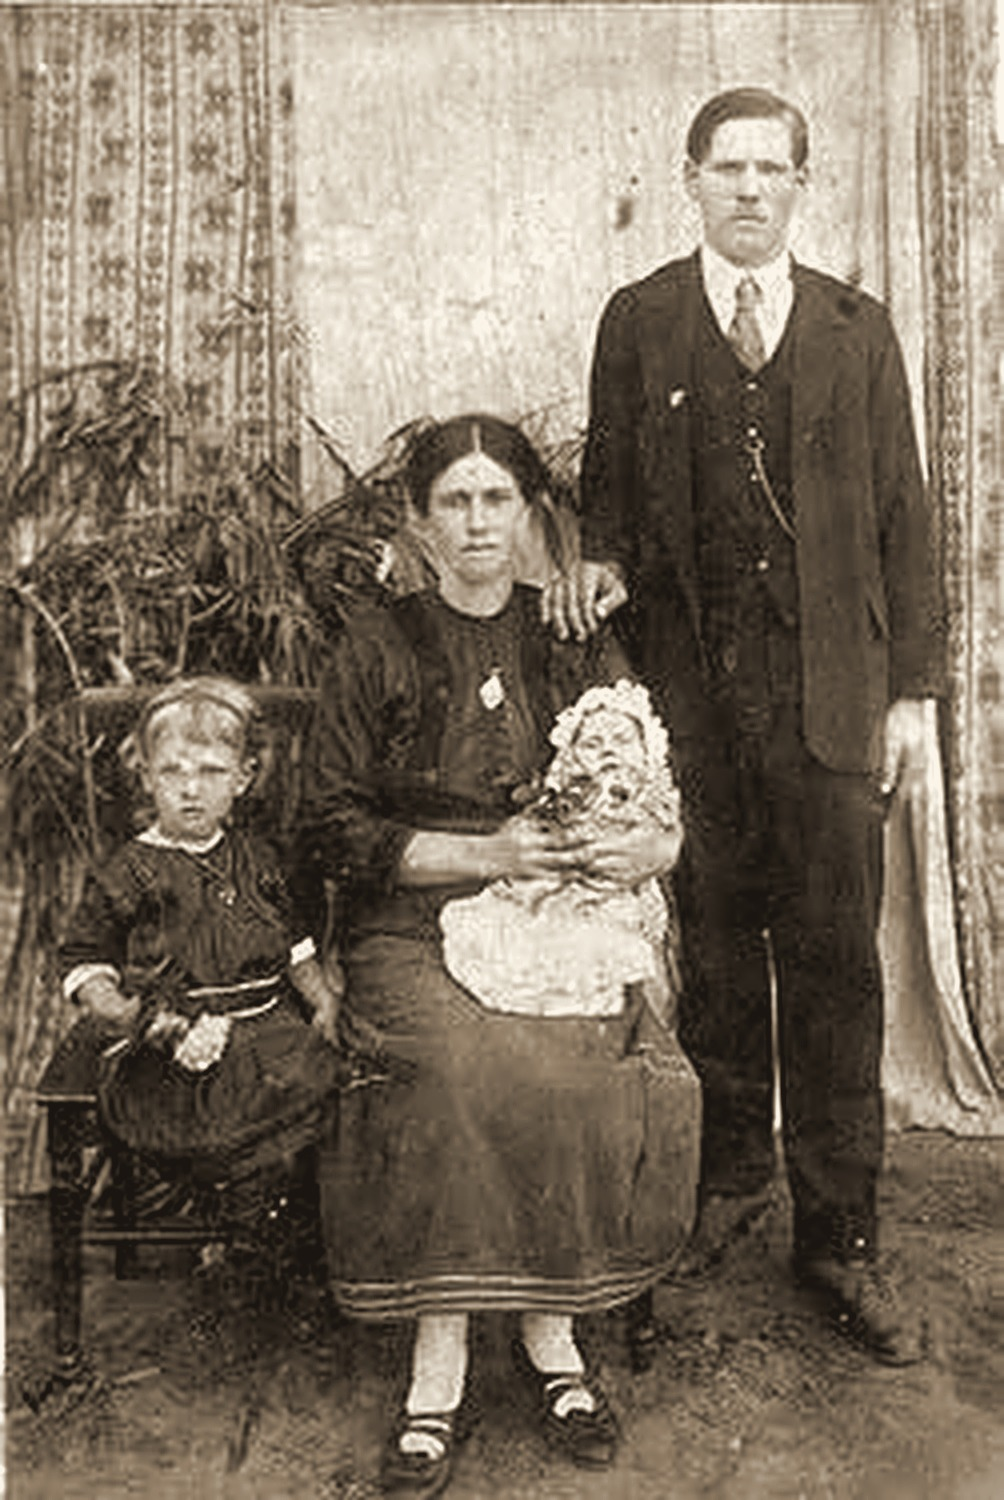
\includegraphics[width=0.6\linewidth,height=\textheight,keepaspectratio,alt={Fernando Dörner und Gertrudes Preiss mit Hilda Ana, die auf dem Stuhl sitzt, und Adelina, meiner Mutter, als Baby auf Gertrudes' Schoß. Um 1927, kurz vor oder kurz nach dem Umzug nach Vidal Ramos. Reproduktion eines kleinen Abzugs, vergrößert und im Kontrast korrigiert; das Original liegt im Repositorium.}]{imagens/doerner_fernando_gertrudes_hilda_adelina_c1927_restaurada.jpg}
\caption{Fernando Dörner und Gertrudes Preiss mit Hilda Ana, die auf dem
Stuhl sitzt, und Adelina, meiner Mutter, als Baby auf Gertrudes' Schoß.
Um 1927, kurz vor oder kurz nach dem Umzug nach Vidal Ramos\index[lugares]{vidal ramos@Vidal Ramos}.
Reproduktion eines kleinen Abzugs, vergrößert und im Kontrast
korrigiert; das Original liegt im Repositorium.}
\end{figure}

Es ist ein Atelierfoto aus dem Landesinneren: ein gemusterter Vorhang,
eine Vase mit Blattpflanzen, ein Stuhl für das Mädchen. Fernando steht,
in dunklem Anzug, mit Weste und Uhrkette, die Hand auf der Schulter
seiner Frau. Er ist etwa dreißig und hat den ernsten Blick eines
Menschen, der nur wenige Male im Leben für einen Fotografen posiert.
Gertrudes sitzt und hält Adelina, die in Weiß gekleidet ist. Hilda Ana,
im dunklen Kleid, schaut direkt in die Kamera. Als das Foto 2017 in den
sozialen Netzwerken herumging, schrieb jemand aus der Familie, das Baby
sei Onkel Lindolfo; aber es ist meine Mutter, und Onkel Lindolfo, damals
etwa zweieinhalb Jahre alt, ist nicht auf dem Bild. Es ist das einzige
Gesicht meines Großvaters, das ich außerhalb der Erinnerung kenne. Für
uns Enkel war er der \emph{Opapa\index[pessoas]{dorner, fernando@Dörner, Fernando}} und Gertrudes die \emph{Omama\index[pessoas]{preiss, gertrudes@Preiss, Gertrudes}}. Falls
ein Vetter oder eine Cousine noch ein anderes Foto von Fernando Dörner\index[pessoas]{dorner, fernando@Dörner, Fernando}
aufbewahrt, vor allem aus den Jahren in Vidal Ramos\index[lugares]{vidal ramos@Vidal Ramos} oder Brusque\index[lugares]{brusque@Brusque}, dann
ist es das Stück, das in diesem Archiv am meisten fehlt.

Auf der Seite der Haas hat der Fata\index[pessoas]{haas, johann@Haas, Johann} sichtbare Spuren des Glaubens
hinterlassen: Er war Kirchenältester in Ituporanga\index[lugares]{ituporanga@Ituporanga} und Erbauer von
Kirchen. Auch Fernando war ein sehr religiöser Mann. Der Artikel von
2011 erzählt, dass er die Erbauer der Kirche, des Pfarrsaals und der
Schule von Vidal Ramos\index[lugares]{vidal ramos@Vidal Ramos} beherbergte und verpflegte, die Estrada da
Igreja, die Kirchstraße, anlegte, Land für den Sportverein Clube
Esportivo Fluminense und für die Schule Escola Cacilda Guimarães
schenkte und mehrere Jahre lang \emph{delegado de polícia} war, also
örtlicher Polizeichef, ohne dafür etwas zu bekommen. Er sagt auch, dass
er ein eifriger Leser war und Zeitschriften abonniert hatte, die nur mit
Mühe an den Ort gelangten. Ich weiß noch nicht, in welchen Jahren er
\emph{delegado} war und wie sich das mit der Geschichte kreuzt, die er
mir erzählt hat.

Die Eltern meiner Mutter gingen nicht direkt von São Martinho\index[lugares]{sao martinho@São Martinho} nach
Brusque\index[lugares]{brusque@Brusque}. Vorher lebten sie in Vidal Ramos\index[lugares]{vidal ramos@Vidal Ramos}, im Alto Vale, der Stadt, in
der ich aufwachsen sollte. Dort geschah diese Geschichte, die kein
Papier der Familie festhält.

Ich habe immer gern den Geschichten älterer Leute zugehört, und das
blieb meiner Mutter nicht verborgen. Als ich schon auf die
weiterführende Schule ging, kam mein Großvater zu uns ins Haus. Er hatte
Hautkrebs, die Krankheit roch schon sehr stark, und er wollte vor seinem
Tod die Angelegenheiten mit den Grundstücken regeln. Eines Tages fragte
ich ihn, wie der Zweite Weltkrieg in Vidal Ramos\index[lugares]{vidal ramos@Vidal Ramos} gewesen sei. Ich fragte
nicht, was er getan hatte. Er selbst spürte, dass er darüber sprechen
musste.

Mein Großvater erzählte mir dann, dass er Hitler unterstützt und in
Milizen von Kolonisten mitgemacht habe, die eine Invasion Südbrasiliens
durch Deutschland unterstützen wollten. Er erzählte auch, dass er die
Seiten gewechselt habe. Nach seinen Worten merkte er beim Lesen von
Zeitschriften wie den \emph{Seleções do Reader's Digest}, dass er auf
der falschen Seite stand. Der Wechsel wurde in Vidal Ramos\index[lugares]{vidal ramos@Vidal Ramos} nicht
akzeptiert. Zusammen mit den Krankheiten meiner Großmutter war er einer
der Gründe, die ihn bewogen, von dort wegzugehen und nach Brusque\index[lugares]{brusque@Brusque} zu
ziehen.

Er sagte, es vergehe kein Tag, an dem er nicht bereue, Hitler
unterstützt zu haben, und das müsse er mit Gott ausmachen. Er sagte
auch, ein Führer wie Hitler übe einen Zauber auf die Menschen aus, und
das werde wieder geschehen. Er starb 1981. Ich weiß nicht, an wen er
dachte, und auch nicht, ob er an jemanden dachte.

Das Wort für das, was er in jenen Jahren war, ist Fünfte Kolonne: der
Bewohner eines Landes, der bereit ist, von innen heraus der Invasion
einer fremden Armee zu helfen. Das Wort ist meines, nicht seines, und
der einzige Beweis, den ich habe, ist das, was er mir selbst gesagt hat.
Er hätte einem Enkel von fünfzehn oder sechzehn Jahren, der nicht einmal
danach gefragt hatte, nichts erzählen müssen. Er erzählte es trotzdem,
krank und dem Tod nahe.

Ich schreibe es so auf, wie ich es bewahrt habe, ohne Szenen
hinzuzufügen und ohne Anführungszeichen zu setzen, wo ich die genauen
Worte nicht habe. Es gibt eine Angabe, die hilft, die Geschichte
zeitlich einzuordnen. Die brasilianische Ausgabe der \emph{Seleções do
Reader's Digest} erschien erstmals im Februar 1942, im Monat nach dem
Abbruch der Beziehungen Brasiliens zu Deutschland, Italien und Japan,
als Teil der amerikanischen Propaganda im Rahmen der Politik der guten
Nachbarschaft. Wenn die Zeitschriften, die er las, die \emph{Seleções}
auf Portugiesisch waren, dann kann der Seitenwechsel nicht vor 1942
liegen. Ich weiß nicht, was für eine Gruppe das war, wer sie
organisierte, wie viele es waren, ob sie Waffen hatten, und auch nicht,
in welchen Jahren er dabei war. Ich weiß nicht, wie die Zeitschriften
nach Vidal Ramos\index[lugares]{vidal ramos@Vidal Ramos} kamen und welche Artikel er las. Das Wort „Miliz`` war
das, das er benutzte, oder das, das ich behalten habe; es kann eine
förmliche Organisation gewesen sein, die mit einer Partei oder einem
Verein verbunden war, oder eine Gruppe von Nachbarn, die sich unterhielt
und übte. Die Geschichte Santa Catarinas in den 1930er- und
1940er-Jahren kennt all das, und es steht mir nicht zu, zu erraten, was
in seinem Fall zutraf. Historiker, die diese Zeit erforscht haben, wie
René Gertz und Marlene de Fáveri, beschreiben den Rahmen, in dem er sich
bewegte: den bis 1937 im Itajaí\index[lugares]{itajai@Itajaí}-Tal starken Integralismus, die
brasilianische faschistische Bewegung; die Ortsgruppen der NSDAP unter
den Deutschbrasilianern bis zum Verbot von 1938; die
Nationalisierungskampagne; und nach 1942 die Angst vor der „Fünften
Kolonne``, die Durchsuchungen, die Verhaftungen und die Spaltungen
innerhalb der Gemeinden selbst. Sie zeigen auch, dass es keinen
deutschen Militärplan für eine Invasion Südbrasiliens gab, auch wenn
viele in den Kolonien daran glaubten, dafür oder dagegen. Nichts davon
sagt, was mein Großvater getan hat. Es sagt nur, dass die Geschichte,
die er mir erzählte, in ihre Zeit passt.

Es war auch nicht der einzige Konflikt. In Vidal Ramos\index[lugares]{vidal ramos@Vidal Ramos} gab es einen
Landstreit, in dem sich mein Großvater gegen die anderen Kolonisten
stellte, und diese Kolonisten wurden schließlich verhaftet. Der Artikel
von 2011 erzählt die Episode genauso, mit mehr Einzelheiten. Viele
Kolonisten weigerten sich, für das Land zu bezahlen, und lehnten sich
gegen die Gesellschaft auf, die es ihnen verkauft hatte. Fernando, der
seines bezahlt hatte, stellte sich auf die Seite der Gesellschaft. Als
die Aufständischen in Brusque\index[lugares]{brusque@Brusque} inhaftiert wurden, war er es, der für die
Familien, die ohne ihre Männer zurückgeblieben waren, die Felder
bestellte, bis die Männer etwa ein Jahr später freikamen, nachdem die
Gesellschaft gesiegt hatte. Ich kenne weder das Jahr noch den Namen der
Gesellschaft noch die Namen der Verhafteten.

Derselbe Artikel erinnert an die andere Seite des Krieges. In der
Kampagne des Estado Novo, des autoritären Regimes von Getúlio Vargas
(1937--1945), gegen die Deutschbrasilianer wurde die Familie als
verdächtig behandelt, und Deutsch zu sprechen und zu lesen wurde zum
belastenden Umstand. Der Großvater, „enttäuscht``, hätte den Enkeln
beinahe verboten, die Sprache zu lernen, um sie zu schützen. Der Artikel
spricht nicht von Milizen. Das öffentliche Gedächtnis der Familie hat
die Verfolgung bewahrt; mir hat er auch erzählt, was davor kam. Beides
kann wahr sein.

Ich kenne das Datum nicht, die Namen nicht und nicht die Seite des
Gesetzes in jedem Moment des Landaufstands. Was ich weiß, ist, dass die
beiden Episoden zusammen gelesen werden müssen, innerhalb einer größeren
Geschichte: der Landkonflikte in den Kolonien, des Misstrauens gegenüber
den Deutschbrasilianern während des Estado Novo und des Krieges, der
Verhaftungen von Kolonisten, der Spaltungen innerhalb der Gemeinden
selbst. Ein Mann, der in der einen Frage die Seiten wechselte und in der
anderen gegen seine Nachbarn stand, verließ Vidal Ramos\index[lugares]{vidal ramos@Vidal Ramos} nicht nur wegen
der Gesundheit seiner Frau.

Ich werde meinen Großvater nicht mit dem richten, was ich heute weiß,
und ihn auch nicht mit dem freisprechen, was ich nicht weiß. Ich tue
lieber, was ein Forscher tut, wenn eine Angabe nicht aufgeht: notieren,
die Quelle suchen und warten. Die Fragen dazu stehen, eine nach der
anderen, in einem eigenen Dokument im Repositorium. Sie richten sich an
Zeitungen der Zeit, an Gerichtsverfahren und polizeiliche
Ermittlungsakten, an die Archive des Bundesstaates und an die Studien
über Nationalsozialismus und Integralismus in Santa Catarina. Wenn
Antworten kommen, gehören sie hierher. Wenn nicht, bleibt, was er mir
erzählt hat. Für den, der zugehört hat, ist auch das eine Quelle: die
eines Mannes, der alt und krank seinem Enkel sagte, dass er sich geirrt
habe, dass er sich geändert habe und dass er es jeden Tag bereue.

\section{Zwei Sterbeurkunden in
Brusque\index[lugares]{brusque@Brusque}}\label{zwei-sterbeurkunden-in-brusque}

\emph{Brusque\index[lugares]{brusque@Brusque}, Santa Catarina, April 1970 und Mai 1981}

Die beiden letzten Dokumente dieses Kapitels sind Sterbeurkunden, und
ich lese sie mit der Sorgfalt, die man einem Familienbrief
entgegenbringt.

Gertrudes starb zuerst. Es war um halb neun am Abend des 9. April 1970,
zu Hause, in Brusque\index[lugares]{brusque@Brusque}. Der Arzt, Dr.~Germano Hoffmann, bescheinigte ein
Karzinom. Der Eintrag wurde am 14. April beim Standesamt aufgenommen,
und wer erschien, um den Tod anzuzeigen, war der Ehemann selbst,
Fernando Doerner, der am Fuß des Eintrags unterschreibt. Die Urkunde
sagt, sie sei aus Imaruí\index[lugares]{imarui@Imaruí} gebürtig gewesen, vierundsiebzig Jahre alt,
Hausfrau, Tochter von Manoel Preus und Helena Michels\index[pessoas]{michels, helena@Michels, Helena}, beide verstorben,
und verheiratet mit Fernando Doerner, mit dem sie sechs volljährige
Kinder hinterließ. Der Standesbeamte schrieb sie der Reihe nach auf:
Hilda Ana, Lindolfo, Adelina, Irma, Olga und Lino Fernando. Das Grab
wurde auf dem katholischen Friedhof der Stadt angelegt.

\begin{figure}
\centering
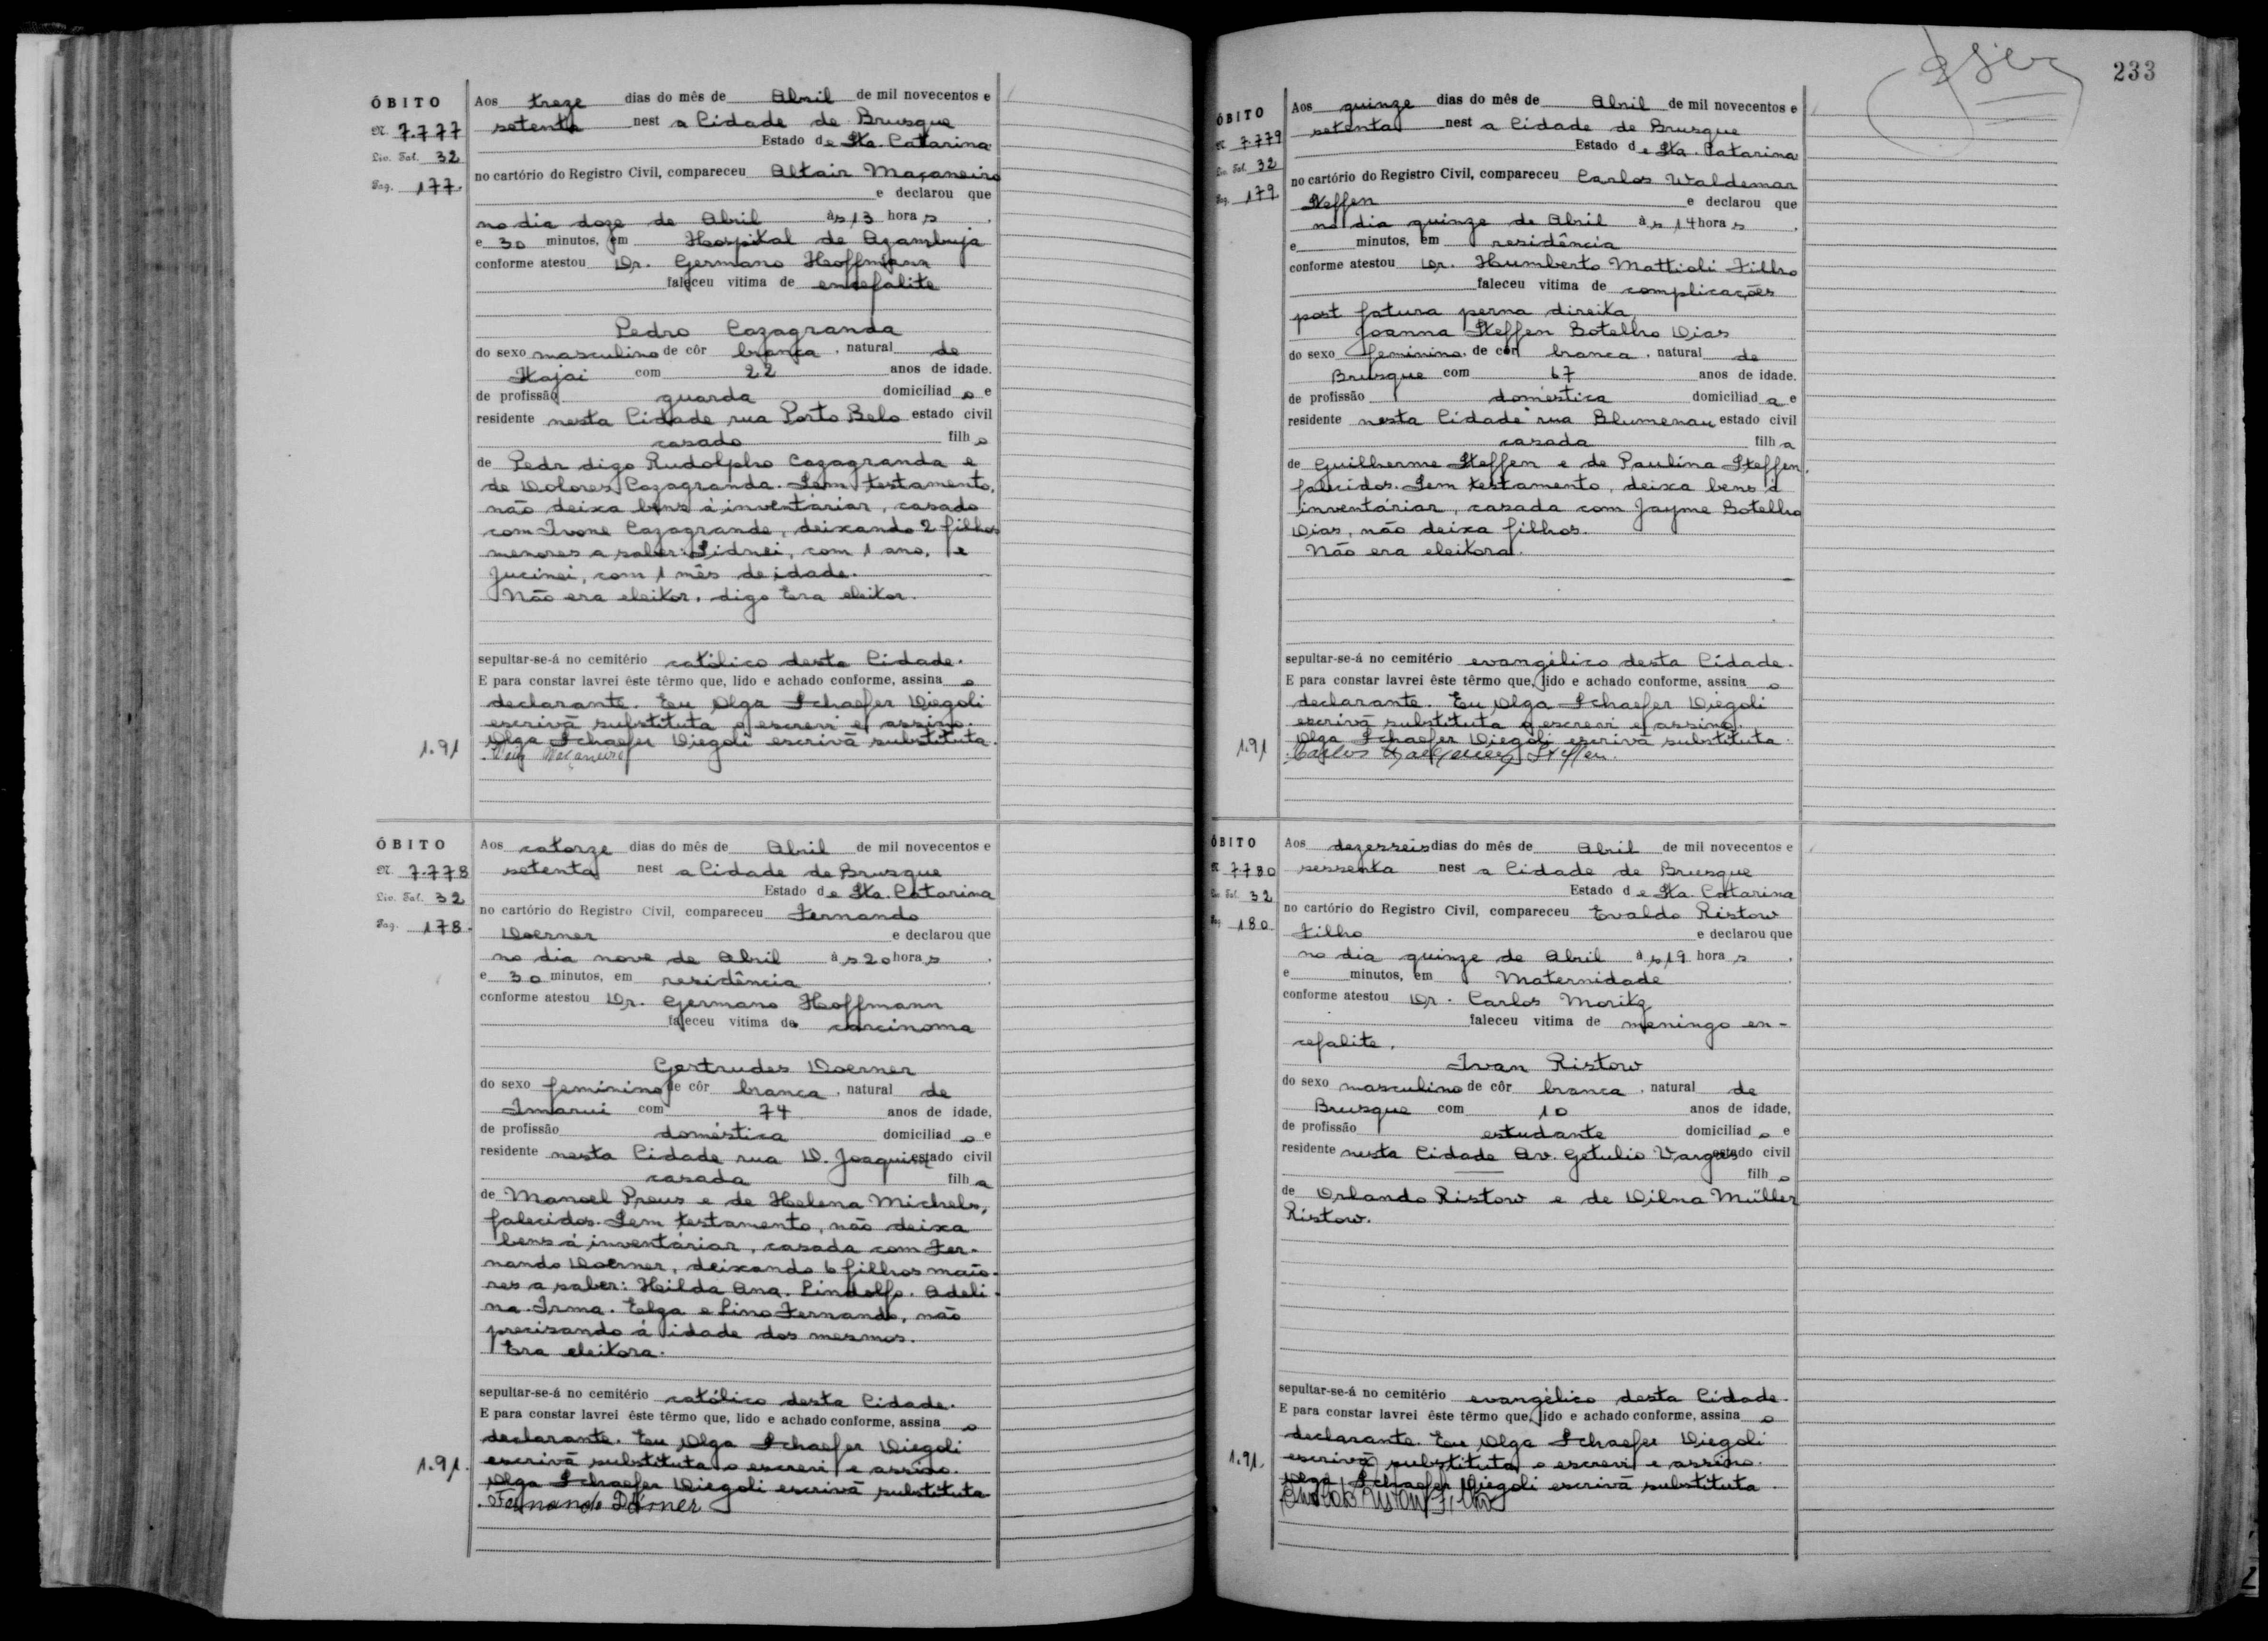
\includegraphics[width=0.85\linewidth,height=\textheight,keepaspectratio,alt={Sterbebuch des Standesamts von Brusque, April 1970: der Eintrag von Gertrudes Doerner (unten links), gebürtig aus Imaruí, 74 Jahre, Tochter von Manoel Preus und Helena Michels, verheiratet mit Fernando Doerner, der den Tod anzeigt und den Eintrag unterschreibt.}]{imagens/doc_doerner_obito_gertrudes_preiss_1970.jpg}
\caption{Sterbebuch des Standesamts von Brusque, April 1970: der Eintrag
von Gertrudes Doerner (unten links), gebürtig aus Imaruí\index[lugares]{imarui@Imaruí}, 74 Jahre,
Tochter von Manoel Preus und Helena Michels\index[pessoas]{michels, helena@Michels, Helena}, verheiratet mit Fernando
Doerner, der den Tod anzeigt und den Eintrag unterschreibt.}
\end{figure}

Ein Detail berührt mich mehr als die anderen. Der Anzeigende ist der
Ehemann. In fast allen Sterbeeinträgen, die ich bei dieser Recherche
gelesen habe, geht ein Sohn, ein Schwiegersohn, ein Nachbar, manchmal
ein Angestellter des Bestattungsunternehmens zum Standesamt. Hier war es
Fernando, mit zweiundsiebzig Jahren, der dem Standesbeamten die Namen
der Schwiegereltern und der sechs Kinder diktierte und unterschrieb. Ich
weiß nicht, ob er es aus Gewohnheit tat, aus Pflichtgefühl oder weil er
es keinem anderen überlassen wollte. Die Unterschrift steht da, am Fuß
von Eintrag 7.778, Blatt 178 von Buch 32.

Fernando lebte noch elf Jahre. Er starb um zehn Uhr morgens am 21. Mai
1981, zu Hause, in Brusque\index[lugares]{brusque@Brusque}, „ohne ärztlichen Beistand``, wie der Eintrag
sagt. Es gab keine ärztliche Bescheinigung, und deshalb nennt der
Eintrag keine Todesursache. Ich hatte ihn kurz zuvor, krank an
Hautkrebs, in unserem Haus gesehen; ich weiß nicht, wann er nach Brusque\index[lugares]{brusque@Brusque}
zurückkehrte. Er war dreiundachtzig Jahre alt. Er war Rentner, gebürtig
aus Imaruí\index[lugares]{imarui@Imaruí}, Witwer, Sohn von Carlos Dörner\index[pessoas]{dorner, carlos@Dörner, Carlos} und Anna Eller\index[pessoas]{eller, anna@Eller, Anna}, beide
verstorben. Er hinterließ fünf volljährige Kinder, kein Testament und
kein Vermögen, über das ein Inventar zu errichten gewesen wäre, was
vielleicht bedeutet, dass die Grundstücke geregelt waren, und er war
Wähler. Er wurde auf dem städtischen Friedhof beigesetzt, den die
Familie als Parque da Saudade kennt.

\begin{figure}
\centering
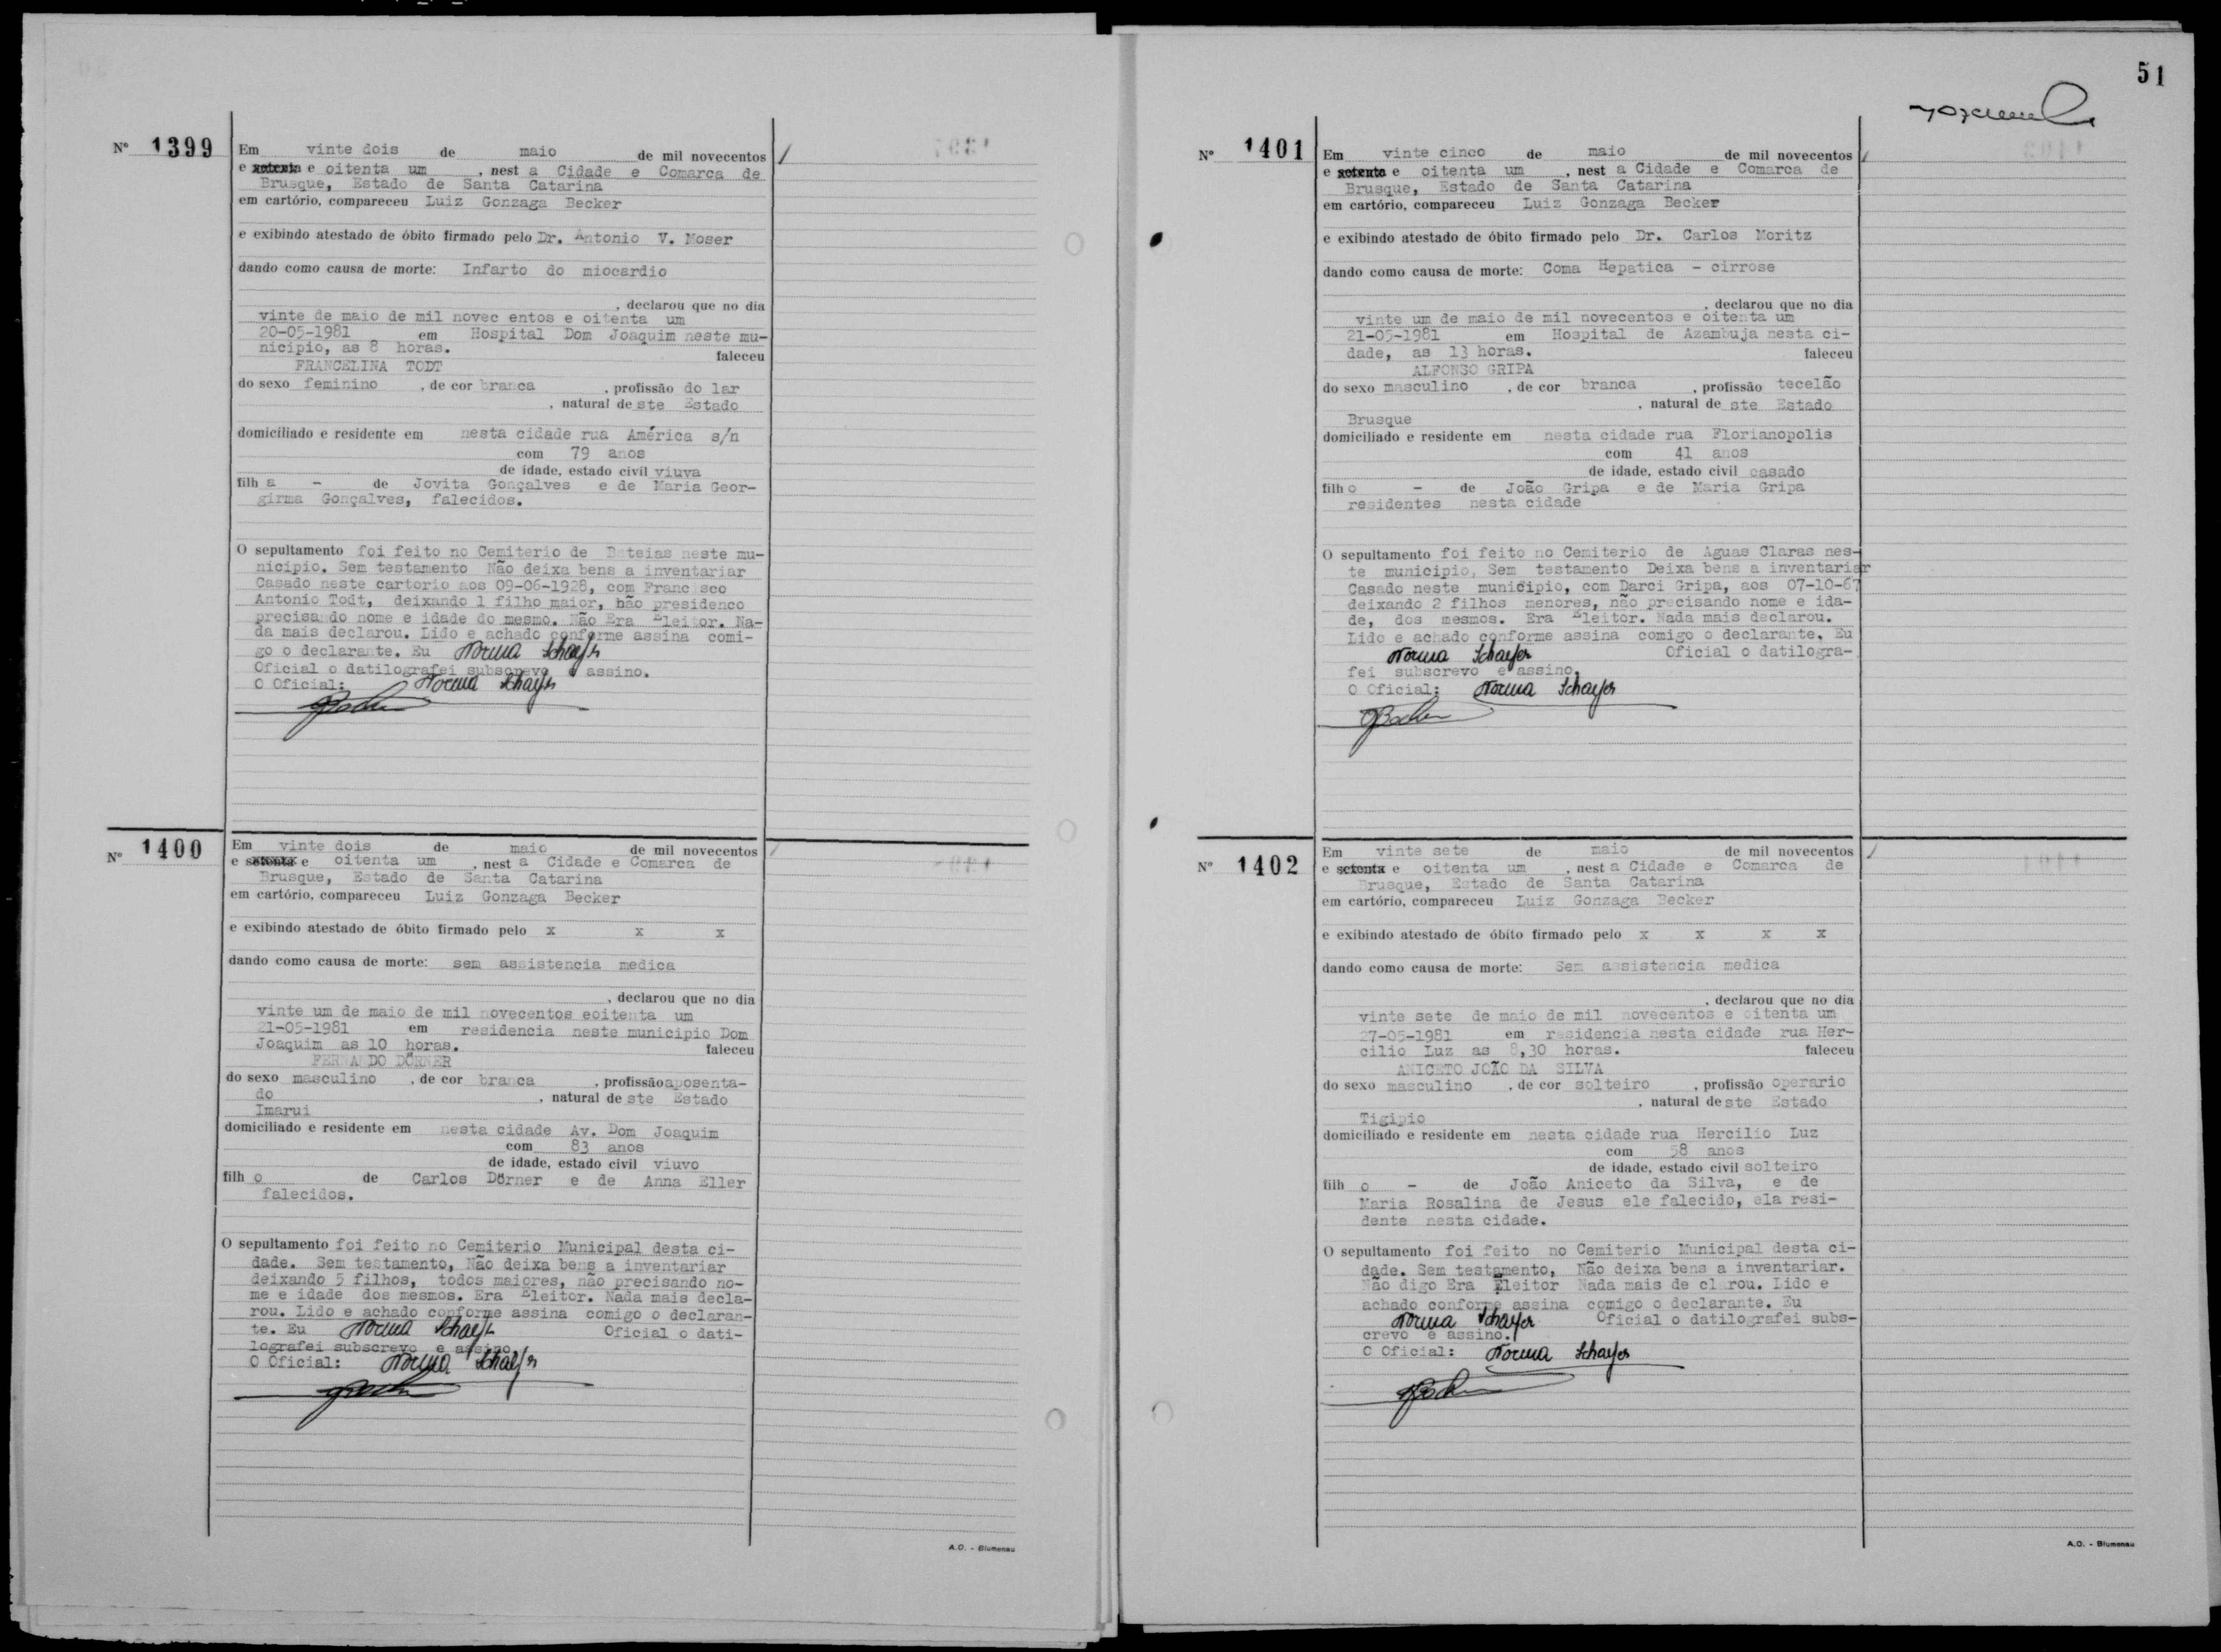
\includegraphics[width=0.85\linewidth,height=\textheight,keepaspectratio,alt={Sterbebuch des Standesamts von Brusque, Mai 1981: Eintrag Nr. 1400 (unten links), Fernando Dörner, 83 Jahre, Rentner, gebürtig aus Imaruí, Witwer, Sohn von Carlos Dörner und Anna Eller.}]{imagens/doc_doerner_obito_fernando_1981.jpg}
\caption{Sterbebuch des Standesamts von Brusque, Mai 1981: Eintrag Nr.
1400 (unten links), Fernando Dörner\index[pessoas]{dorner, fernando@Dörner, Fernando}, 83 Jahre, Rentner, gebürtig aus
Imaruí\index[lugares]{imarui@Imaruí}, Witwer, Sohn von Carlos Dörner\index[pessoas]{dorner, carlos@Dörner, Carlos} und Anna Eller\index[pessoas]{eller, anna@Eller, Anna}.}
\end{figure}

\begin{ficha}

\textbf{Archivkarte}: (1) Sterbeeintrag von Gertrudes Doerner,
Standesamt Brusque\index[lugares]{brusque@Brusque}, Buch 32, Bl. 178, Eintrag Nr. 7.778, aufgenommen am
14.04.1970; Tod am 09.04.1970, 20.30 Uhr, in der Wohnung; Bescheinigung
von Dr.~Germano Hoffmann, Karzinom; gebürtig aus Imaruí\index[lugares]{imarui@Imaruí}, 74 Jahre;
Tochter von Manoel Preus und Helena Michels\index[pessoas]{michels, helena@Michels, Helena}; Anzeigender: Fernando
Doerner; sechs volljährige Kinder: Hilda Ana, Lindolfo, Adelina, Irma,
Olga und Lino Fernando; Grab auf dem katholischen Friedhof von Brusque\index[lugares]{brusque@Brusque}.
(2) Sterbeeintrag von Fernando Dörner\index[pessoas]{dorner, fernando@Dörner, Fernando}, Standesamt Brusque\index[lugares]{brusque@Brusque}, Eintrag Nr.
1400, aufgenommen am 22.05.1981; Tod am 21.05.1981, 10 Uhr, in der
Wohnung, „ohne ärztlichen Beistand``; gebürtig aus Imaruí\index[lugares]{imarui@Imaruí}, 83 Jahre,
Rentner, Witwer; Sohn von Carlos Dörner\index[pessoas]{dorner, carlos@Dörner, Carlos} und Anna Eller\index[pessoas]{eller, anna@Eller, Anna}; fünf volljährige
Kinder; Grab auf dem städtischen Friedhof. Dateien:
\texttt{imagens/doc\_doerner\_obito\_gertrudes\_preiss\_1970.jpg} und
\texttt{imagens/doc\_doerner\_obito\_fernando\_1981.jpg}.

\end{ficha}

Zwei Beobachtungen des Forschers. Die erste: Beide Dokumente sagen
„gebürtig aus Imaruí\index[lugares]{imarui@Imaruí}`` und nicht São Martinho\index[lugares]{sao martinho@São Martinho}, wie FamilySearch. Das ist
kein Widerspruch, denn als sie geboren wurden, gehörte São Martinho\index[lugares]{sao martinho@São Martinho} zu
Imaruí\index[lugares]{imarui@Imaruí}, und der Standesbeamte in Brusque\index[lugares]{brusque@Brusque} schrieb den Namen der damaligen
Gemeinde auf. So ein Detail wirkt klein, aber wer Taufeinträge in den
falschen Büchern sucht, verliert seinetwegen Monate. Die zweite: 1970
lebten sechs Kinder, 1981 waren es fünf. Zwischen dem einen Eintrag und
dem anderen starb eines der Kinder von Fernando und Gertrudes. Die
beiden Urkunden sagen nicht, welches, aber das Standesamtsregister von
Brusque\index[lugares]{brusque@Brusque} sagt es: Lino Fernando, der Jüngste der Überlebenden, starb am
14. Februar 1979 mit einundvierzig Jahren. Fernando begrub einen Sohn
zwei Jahre vor seinem eigenen Tod.

Brusque\index[lugares]{brusque@Brusque} ist eine Flussstadt. Sie entstand 1860 als Colônia Itajahy am
Ufer des Itajaí\index[lugares]{itajai@Itajaí}-Mirim, des kleineren Arms des großen Flusses, der das
Tal durchzieht. Das Wasser war, wie in allen Kolonien, Straße, Energie
und Gefahr. Es trieb die ersten Webereien an, die der Stadt ihren Ruf
gaben, und stieg von Zeit zu Zeit bis in die Häuser. Fernando starb im
Mai 1981. Drei Jahre später, im August 1984, überschwemmte eines der
großen Hochwasser des Itajaí\index[lugares]{itajai@Itajaí}-Tals Brusque\index[lugares]{brusque@Brusque}. Weitere kamen im November
2008, bei der Katastrophe, die in Santa Catarina etwa
hundertfünfunddreißig Menschen tötete, und 2011. Jedes Mal kam dieselbe
Kombination zusammen: anhaltender Regen, der vom Meer gegen den Hang des
Küstengebirges zog, ein enger, zwischen Hügeln eingeschnittener Fluss
und eine Stadt, die dort gebaut ist, wo das Wasser schon immer floss.
Ich arbeite mit Hochwassermodellen für den Itajaí\index[lugares]{itajai@Itajaí}, und wenn ich die
Karte der Überschwemmungsgebiete von Brusque\index[lugares]{brusque@Brusque} öffne, suche ich fast
unwillkürlich die Straße, in der meine Großeltern wohnten. Ihren Namen
schreibe ich hier nicht. Es genügt zu sagen, dass sie, hätten sie etwas
länger gelebt, gesehen hätten, wie der Fluss in die Stadt kam, so wie er
ins ganze Tal kam. In Kapitel 13 komme ich auf diese Flüsse zurück, die
am Ende ein einziges Problem sind.

Manchmal denke ich an den Abstand zwischen dem ersten und dem letzten
Dokument dieses Kapitels. Auf der einen Seite das Rheinland der
Schmieden, wo um 1854 ein Junge geboren wird. Auf der anderen ein
Standesamt in Brusque\index[lugares]{brusque@Brusque} im Jahr 1981, wo sein Sohn, schon alt, als
„Rentner`` und „Wähler`` eingetragen wird, zwei Wörter, die sich kein
Dörner in Solingen\index[lugares]{solingen@Solingen} neben seinem eigenen Namen hätte vorstellen können.
Der Weg zwischen diesen beiden Punkten führt über das Westfalen\index[lugares]{westfalen@Westfalen} der
Eller, über zehn Kinder einer Frau, die früh starb, über eine Kapelle in
Capivari\index[lugares]{capivari@Capivari}, wo zwei Christen von vielleicht verschiedenen Konfessionen
eine Dispens brauchten, um zu heiraten, über fünf weitere Kinder einer
anderen Mutter, über einen Jüngsten, der seine eigene nie kannte, und
über eine junge Frau, die von den Schiffen des Jahres 1828 abstammte.
Aus diesem Weg ging Adelina hervor, und aus Adelina ging ich hervor.

Mit diesem Kapitel schließe ich den väterlichen Teil eures Stammbaums.
Von der Seite meines Vaters und meiner Mutter hatten wir schon vier
Jahrhunderte Geschichte. Es fehlte die andere Hälfte meiner Söhne.

\section{Für euch zum Entdecken}\label{fuxfcr-euch-zum-entdecken-9}

\begin{itemize}
\tightlist
\item
  Gibt es eine zweite Ausfertigung von Eintrag Nr. 23 im Buch der
  Mutterpfarrei? Und woher stammt die alte Abschrift mit Padre Auling
  und der Dispens?
\item
  In welchem Jahr und auf welchem Schiff fuhr Carlos Dörner\index[pessoas]{dorner, carlos@Dörner, Carlos} über den
  Ozean, und wurde er wirklich in Solingen\index[lugares]{solingen@Solingen} geboren? Kein Dokument, das
  ich habe, gibt darauf Antwort.
\item
  Was für eine Gruppe war das, bei der mein Großvater Fernando
  mitmachte, wer organisierte sie und in welchen Jahren? Die Fragen
  stehen in einem eigenen Dokument im Repositorium und richten sich an
  Zeitungen der Zeit, an Gerichtsverfahren und polizeiliche
  Ermittlungsakten und an die Archive des Bundesstaates.
\item
  Als mein Großvater sagte, der Zauber eines Führers wie Hitler werde
  wieder geschehen, wovon sprach er? Schaut euch eure eigene Zeit an und
  entscheidet, ob er recht hatte.
\item
  Bewahrt ein Vetter oder eine Cousine noch ein anderes Foto von
  Fernando Dörner\index[pessoas]{dorner, fernando@Dörner, Fernando} auf, vor allem aus den Jahren in Vidal Ramos\index[lugares]{vidal ramos@Vidal Ramos} oder
  Brusque\index[lugares]{brusque@Brusque}? Fragt auch die Verwandten in Vidal Ramos\index[lugares]{vidal ramos@Vidal Ramos}, was man sich über
  den Landaufstand erzählt: das Jahr, die Gesellschaft, die Verhafteten.
\end{itemize}

\part{Bárbaras Horizonte}\label{buxe1rbaras-horizonte}

\begin{boletim}

Feuchte Luft steigt im Taquari-Tal auf. Beständige Strömungen zwischen
Joinville\index[lugares]{joinville@Joinville}, Estrela\index[lugares]{estrela@Estrela} und Arroio do Meio\index[lugares]{arroio do meio@Arroio do Meio}. Mikroklimate einer Familie.

\end{boletim}

\chapter{In der Garage von Oma Rosita, in den Bildern von Opa Erno und
im Vermächtnis von Dr.~Carlos Heinz Funke\index[pessoas]{funke, carlos heinz@Funke, Carlos Heinz}}\label{cap-11}

\begin{quote}
\emph{Es gibt Häuser, in denen Weihnachten mit dem Duft von Plätzchen
beginnt. In einem davon wartete die andere Hälfte dieser Geschichte auf
mich.}
\end{quote}

\emph{26,3° S · 48,8° W, Joinville\index[lugares]{joinville@Joinville}, SC}

\section{Vier Generationen in einer
Garage}\label{vier-generationen-in-einer-garage}

Auf dem Foto, das dieses Kapitel eröffnet, sind fünf Menschen zu sehen,
und die Bildunterschrift der Familie nennt nur vier beim Namen. Das Bild
ist das Foto eines Fotos. Jemand hat mit dem Handy eine Albumseite
fotografiert und dabei, ohne es zu wollen, oben im Bild ein Stück der
vorigen Seite mit aufgenommen: einen weißen Dachvorsprung, einen sehr
blauen Himmel und zwei dunkle Vögel, die auf der Dachrinne sitzen.
Darunter, geschützt von der Plastikfolie des Albums, ist die Szene, auf
die es ankommt. Es ist eine Garage in Joinville\index[lugares]{joinville@Joinville}, Anfang 2005. Hinten
eine Holztür und ein dunkles Auto, und draußen das Grün eines Gartens.

Nach der Bildunterschrift, die die Familie dazu geschrieben hat, sind
dort vier Generationen versammelt. Die Urgroßmutter Oma Rosita\index[pessoas]{lohmann, rosita erica@Lohmann, Rosita Érica} Lohmann
Hoeveler, mit weißem Haar und geblümtem Kleid, auf einen Rollator aus
Aluminium gestützt. Ihre Enkelin Bárbara, im bedruckten Kleid, mit dem
runden Bauch einer Frau, die ihr zweites Kind erwartet. Dieses Kind bist
du, Lucas, der am 10. März jenes Jahres zur Welt kommen sollte. Und die
Großmutter, Dra. Ilusca Leocádia Hoeveler Funke, mit einem blonden
Jungen im blauen T-Shirt auf dem Arm: Das bist du, Matheus, geboren am
20. Juni 2002. Durch einen Zufall, der mich immer wieder amüsiert, bist
du am selben Tag geboren wie ich. Ich bekam ein Geburtstagsgeschenk mit
siebenunddreißig Jahren Verspätung.

\begin{figure}
\centering
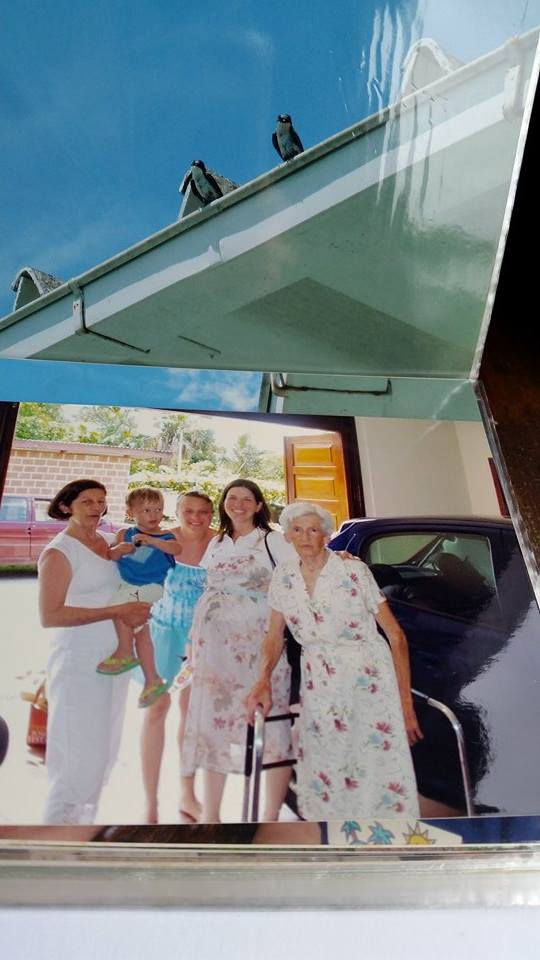
\includegraphics[width=0.85\linewidth,height=\textheight,keepaspectratio,alt={Vier Generationen in der Garage des Familienhauses in Joinville, Anfang 2005: die Urgroßmutter Oma Rosita Lohmann Hoeveler mit dem Rollator; Bárbara Funke Haas, schwanger mit Lucas; und die Großmutter Dra. Ilusca Leocádia Hoeveler Funke mit Matheus auf dem Arm. Das Bild ist die Reproduktion einer Albumseite.}]{imagens/lohmann_4_geracoes_oma_rosita_ilusca_barbara_matheus.jpg}
\caption{Vier Generationen in der Garage des Familienhauses in
Joinville\index[lugares]{joinville@Joinville}, Anfang 2005: die Urgroßmutter Oma Rosita\index[pessoas]{lohmann, rosita erica@Lohmann, Rosita Érica} Lohmann Hoeveler mit
dem Rollator; Bárbara Funke Haas, schwanger mit Lucas; und die
Großmutter Dra. Ilusca Leocádia Hoeveler Funke mit Matheus auf dem Arm.
Das Bild ist die Reproduktion einer Albumseite.}
\end{figure}

Ich mag dieses Bild wegen dessen, was es zeigt, und wegen dessen, was es
verbirgt. Es zeigt eine Linie von Frauen: Rosita, 1918 im Vale do
Taquari in Rio Grande do Sul geboren; Ilusca, die zwischen Estrela\index[lugares]{estrela@Estrela} und
Nova Petrópolis\index[lugares]{nova petropolis@Nova Petrópolis} aufwuchs; Bárbara, am 27. Juli 1972 in Porto Alegre
geboren und in Joinville\index[lugares]{joinville@Joinville} aufgewachsen. Es verbirgt fast alles, was vor
ihnen kam: die Segelschiffe von 1846, einen Hof von vierundzwanzig
Kolonien, eine Frau, die sechsundzwanzig Tage nach einer Geburt starb,
ein neues Haus in Palmas\index[lugares]{palmas@Palmas}, gegenüber dem Salto do Taquari. Nichts davon
ist auf dem Foto zu sehen, aber all das war darin, stand an einem
Sommertag in einer Garage. Die fünfte Person, eine junge Frau im blauen
Kleid, nennt die Bildunterschrift nicht, und ich lasse es dabei.

In den vorigen Kapiteln bin ich den Strömen gefolgt, die in mir
zusammenfließen: den Haas und den Meier aus Bayern\index[lugares]{bayern@Bayern}, den Doerner, den
Preiss, den Michels und den Arns. Jetzt muss ich tun, was ein
Meteorologe tut, wenn er merkt, dass seine Rückwärtstrajektorie nur die
Hälfte der Feuchtigkeit eines Gewitters erklärt hat: die andere Quelle
suchen. Matheus und Lucas sind nicht nur Haas. Sie sind auch Funke,
Hoeveler, Lohmann, Endres, Schnack und Wingert. Diese Hälfte kann ich
nicht allein erzählen.

Deshalb spricht in diesem Teil IV auch Bárbara. Die kursiven Abschnitte,
die immer mit ihrem Namen eingeleitet werden, sind von ihr, in der
ersten Person. Der Rest bleibt meine Stimme, die Stimme dessen, der von
außen in diese Familie kam, als Schwiegersohn, und die Namen nach und
nach lernte.

\section{Die andere Hälfte}\label{die-andere-huxe4lfte}

Joinville\index[lugares]{joinville@Joinville} hat ein Klima, das ich als Meteorologe immer theatralisch
fand. Die Stadt liegt eingezwängt zwischen der Baía da Babitonga im
Osten und der Mauer der Serra do Mar im Westen, die dort Serra Dona
Francisca heißt. Die feuchte Luft vom Ozean wird gegen den Hang
gedrückt, steigt auf, kühlt ab und gibt ihre Feuchtigkeit als Regen ab.
Deshalb regnet es so viel in Joinville\index[lugares]{joinville@Joinville}. Es ist eine der regenreichsten
Städte Südbrasiliens, mit ganzen Tagen voller Nieselregen und
Sommernachmittagen, an denen der Regen ohne jede Vorwarnung schwer
herunterkommt. Die Kolonisten, die 1851 ankamen, um die Colônia Dona
Francisca zu gründen, lernten das schnell. Ihre Nachkommen haben bis
heute die Gewohnheit, einen Regenschirm neben der Tür stehen zu haben.

In dieser Stadt zwischen Meer und Gebirge ließen sich die Funke nieder,
und hierher kamen später die Hoeveler aus Rio Grande do Sul. Bárbaras
Vater, der Arzt Carlos Heinz Funke\index[pessoas]{funke, carlos heinz@Funke, Carlos Heinz}, wurde dort am 10. August 1939
geboren. Die Mutter, Ilusca, kam aus Rio Grande. Ich weiß nicht, und ich
werde es nicht erfinden, wo und wie die beiden sich kennenlernten. Er
studierte Medizin in Rio Grande do Sul, und das Universitätsleben in
Porto Alegre oder in der Umgebung ist der wahrscheinlichste Schauplatz,
aber das ist nur eine Hypothese. Ich weiß, dass sie heirateten, dass sie
vier Kinder hatten (Bárbara, Katherine, Alessandra und Paulo Jacques)
und dass Oma Rosita\index[pessoas]{lohmann, rosita erica@Lohmann, Rosita Érica} ihre letzten Jahre in ihrer Nähe verbrachte, in
Joinville\index[lugares]{joinville@Joinville}.

Die Funke bringen eine Überraschung mit, die ich erst sah, als ich die
beiden Stammbäume zusammenlegte. In den Einträgen bei FamilySearch sind
Paulo Funke\index[pessoas]{funke, paulo@Funke, Paulo} und Hulda, Bárbaras Urgroßeltern, 1881 und 1889 in Glauchau\index[lugares]{glauchau@Glauchau}
in Sachsen\index[lugares]{sachsen@Sachsen} geboren, und ihr Sohn Oscar Martin, Bárbaras Großvater, kam
am 1. Dezember 1910 im Bezirk Glauchau\index[lugares]{glauchau@Glauchau} zur Welt. Glauchau liegt wenige
Dutzend Kilometer von Chemnitz\index[lugares]{chemnitz@Chemnitz} entfernt. Und Chemnitz ist die Stadt, in
der nach der Erinnerung meiner Familie der Fata\index[pessoas]{haas, johann@Haas, Johann} und die Mota\index[pessoas]{meier, maria@Meier, Maria} lebten,
bevor sie 1913 aufbrachen. Um 1910 ist es also möglich, dass die
Urgroßeltern auf meiner Seite und die von Bárbara in derselben Gegend
Sachsens lebten, ohne voneinander zu wissen, und dass sie alle am Ende
in Santa Catarina landeten. Kein Papier sagt, dass sie sich begegnet
sind. Und es gibt noch einen Zweig weit weg von dort: Dora Marta, die
Oma Dora\index[pessoas]{aenishaenslin, dora marta@Aenishaenslin, Dora Marta}, war die Tochter von Jacques Aenishaenslin\index[pessoas]{aenishaenslin, jacques@Aenishaenslin, Jacques}, der in der Schweiz
geboren war, in einer Familie aus Ormalingen\index[lugares]{ormalingen@Ormalingen} bei Basel.

Als ich Bárbara heiratete, fügte ich meinem Stammbaum einen Zweig hinzu,
den ich nicht kannte. Auf meiner Seite Katholiken aus Bayern\index[lugares]{bayern@Bayern}, von der
Mosel\index[lugares]{mosel@Mosel} und aus dem Rheinland. Auf ihrer Seite Lutheraner aus
Braunschweig, aus Schleswig-Holstein, aus der evangelischen Tradition
des Vale do Taquari und der Serra Gaúcha. Auf meiner Seite Leute, die
mit ihren Händen Kirchen bauten. Auf ihrer Seite Leute, die lehrten und
heilten. Ich will daraus keine Formel machen, denn Familien sind
gemischter als jede Zusammenfassung, aber der Gegensatz ist da, und ich
habe ihn seit den ersten Sonntagsessen in Joinville\index[lugares]{joinville@Joinville} gespürt.

Hier gebe ich Bárbara das Wort.

\emph{In meiner Erinnerung gehört Oma Rosita\index[pessoas]{lohmann, rosita erica@Lohmann, Rosita Érica} so sehr zum Haus in
Joinville\index[lugares]{joinville@Joinville} wie die Küche. Sie kam aus Rio Grande, aus einer Familie mit
zwölf Geschwistern, und ich habe lange gebraucht, um zu verstehen, was
das bedeutete. Wenn sie von ihren Geschwistern sprach, klangen die Namen
wie die von Romanfiguren: Urbano, Armando, Sunta, Arlindo. Lange waren
sie für mich mehr Namen als Gesichter: Leute, die weit weg lebten, in
einem Tal, das sie vor langer Zeit verlassen hatte.}

\emph{Der Name, der mich am unmittelbarsten mit ihr verbindet, ist nicht
einmal meiner, sondern der meiner Mutter. Ilusca Leocádia. Das Leocádia
kam von der Urgroßmutter, Miguelina Leocádia Endres\index[pessoas]{endres, miguelina leocadia@Endres, Miguelina Leocádia}, der Mutter von Oma
Rosita. In unserer Familie werden die Namen so weitergegeben, nach
innen, im zweiten Vornamen, wie etwas, das man nicht ankündigt, das aber
auch nicht verloren geht.}

\section{Der Arzt von Pirabeiraba}\label{der-arzt-von-pirabeiraba}

Dr.~Carlos Heinz Funke\index[pessoas]{funke, carlos heinz@Funke, Carlos Heinz}, der in den Dokumenten mal als Heinz, mal als
Heins erscheint, starb 1989 in Joinville\index[lugares]{joinville@Joinville}, mit etwa fünfzig Jahren.
Bárbara war damals ein Teenager. Ich habe ihn nicht gekannt. Ich weiß
von ihm, was die Familie erzählt und was die Stadt bewahrt hat, und die
Stadt hat einiges bewahrt.

In Pirabeiraba\index[lugares]{pirabeiraba@Pirabeiraba}, dem ländlichen Distrikt nördlich von Joinville\index[lugares]{joinville@Joinville} am Fuß
des Gebirges, tragen zwei öffentliche Einrichtungen seinen Namen. Die
eine ist die Gesundheitsstation Unidade Básica de Saúde da Família
Dr.~Carlos Heinz Funke\index[pessoas]{funke, carlos heinz@Funke, Carlos Heinz}. Die andere ist die städtische
Landwirtschaftsschule Escola Agrícola Municipal Carlos Heins Funke,
gegründet 1989, im Jahr seines Todes, und am 15. Februar 1990 zum
Betrieb zugelassen.

\begin{ficha}

\textbf{Archivkarte}: Escola Agrícola Municipal Carlos Heins Funke,
Pirabeiraba\index[lugares]{pirabeiraba@Pirabeiraba}, Joinville\index[lugares]{joinville@Joinville} (SC). Gegründet 1989 durch das Dekret Nr. 6168/89
und das Gutachten 452/89; Betrieb zugelassen am 15.02.1990; der Eltern-
und Lehrerverein (APP) wurde durch das Gesetz Nr. 3.968 vom 05.07.1999
als gemeinnützig anerkannt. Die Schule bietet die Sekundarstufe I
(\emph{ensino fundamental}, 6. bis 9. Schuljahr) mit
landwirtschaftlicher Vorqualifizierung an, als Ganztagsschule, für
Schüler aus der ganzen Gemeinde. Quelle: institutionelle Seite des
Eltern- und Lehrervereins der Schule (abgerufen 2026).

\end{ficha}

Ich stelle mir gern vor, was dieser Name an einer Landwirtschaftsschule
einem Mann gesagt hätte, der sein Leben zwischen Sprechzimmern und
Krankenhäusern verbracht hat. Die Seite der Schule erklärt, das Ziel
sei, die Jugendlichen auf die Arbeit im landwirtschaftlichen Betrieb der
Familie vorzubereiten, „indem man das Interesse am Verbleiben auf dem
Land weckt``. Das ist fast eine Antwort, hundert Jahre später, auf das
Drama aller Familien dieses Buches, die zu viele Kinder für das
vorhandene Land hatten und sie fortgehen sahen. Ich weiß nicht, ob
Dr.~Carlos Heinz jemals daran gedacht hat. Ich weiß, dass die Namen, die
eine Stadt ihren Schulen und Gesundheitsstationen gibt, eine Art sind zu
sagen, wer sich um sie gekümmert hat.

Von seiner Familie habe ich zwei Fotos, und beide verlangen eine
vorsichtige Lesung.

Das erste ist ein Atelierporträt in Sepia, vom Alter fleckig, das die
Familie als „der Urgroßvater und die Familie von Oma Dora\index[pessoas]{aenishaenslin, dora marta@Aenishaenslin, Dora Marta}`` aufbewahrt.
Oma Dora\index[pessoas]{aenishaenslin, dora marta@Aenishaenslin, Dora Marta} ist die Mutter von Dr.~Carlos Heinz, Bárbaras Großmutter
väterlicherseits. In der Mitte sitzen ein Mann mit Schnurrbart, hellem
Anzug und Weste und eine Frau in einem weißen Kleid mit breitem Kragen,
die Hände im Schoß. Um sie herum neun junge Leute: junge Männer mit
Krawatte, junge Frauen mit kurzem Haar nach der Mode der späten
1920er-Jahre, ein Mädchen mit geradem Pony, ein Junge mit offenem
Kragen. Wenn ich richtig gezählt habe, sind es neun Kinder. Die
Zuordnung der einzelnen Gesichter, auch die von Dora, muss noch mit
jemandem bestätigt werden, der sie kennt, und ich wage sie nicht.

\begin{figure}
\centering
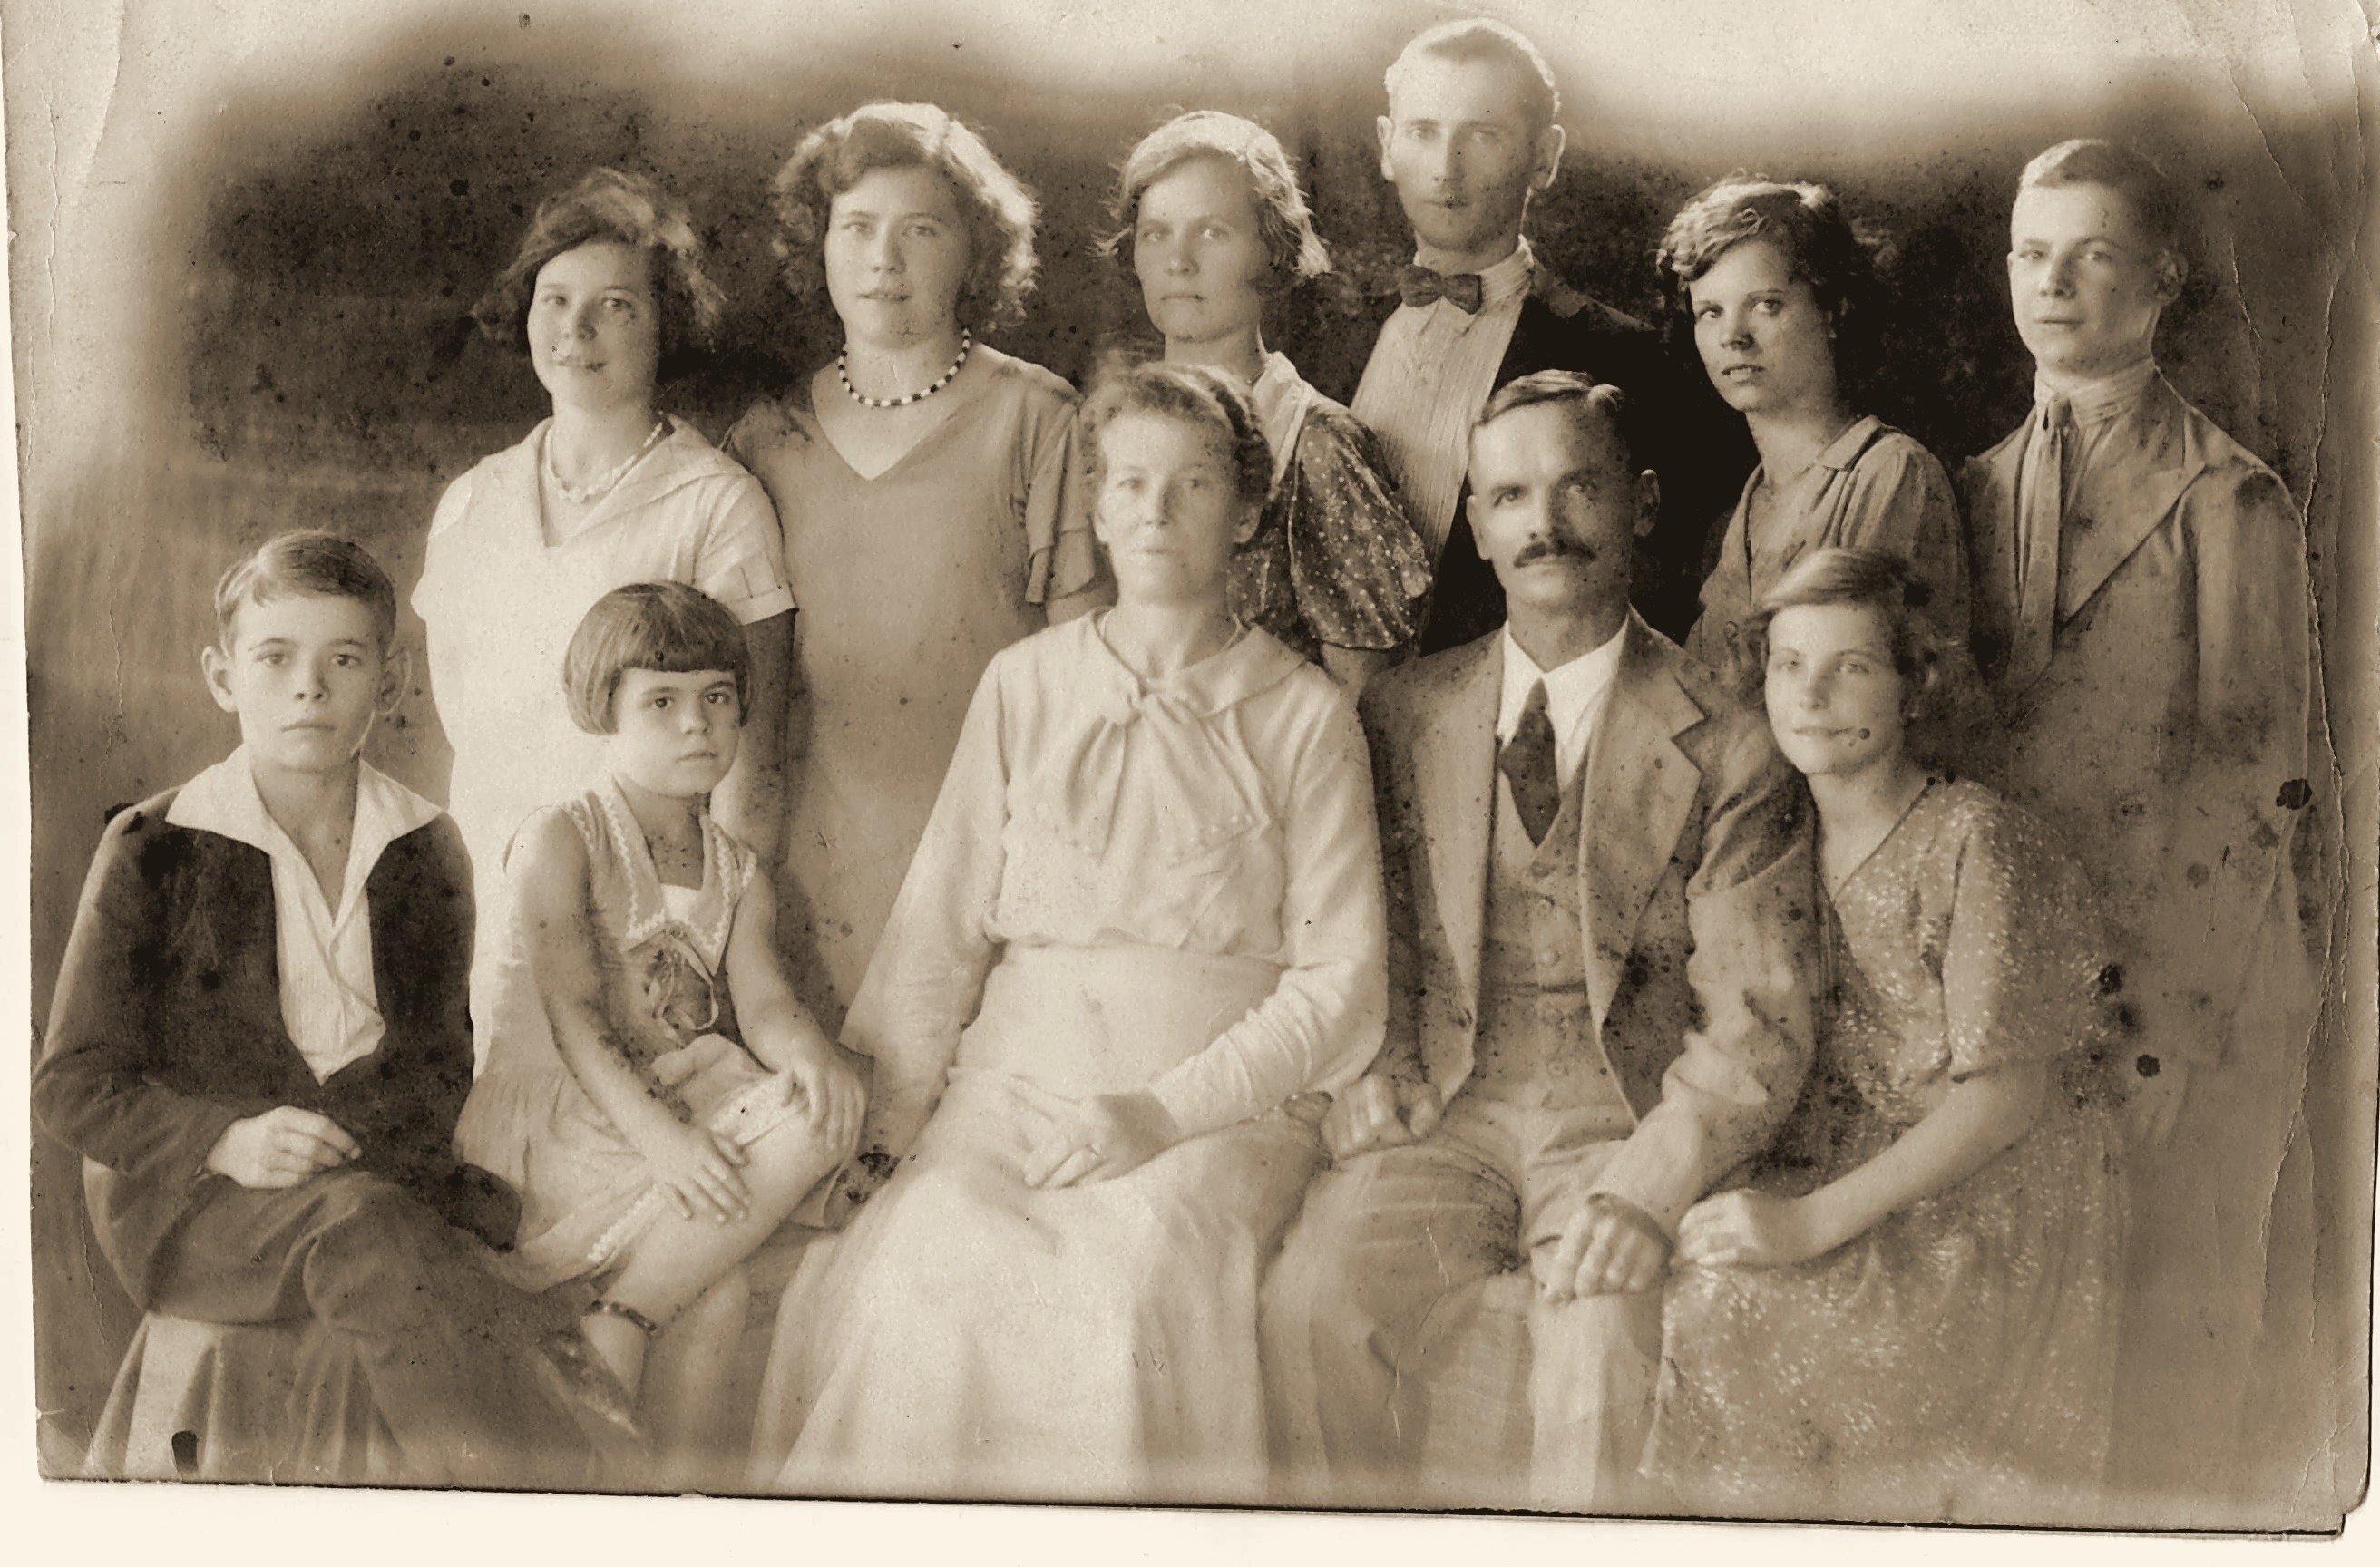
\includegraphics[width=0.85\linewidth,height=\textheight,keepaspectratio,alt={Familienporträt in Sepia, aufbewahrt als „der Urgroßvater und die Familie von Oma Dora``: das Ehepaar sitzend in der Mitte, umgeben von den Kindern, wahrscheinlich Ende der 1920er- oder Anfang der 1930er-Jahre. Die Zuordnung der einzelnen Personen steht noch aus. Kontrast und Töne korrigiert.}]{imagens/funke_bisavo_e_familia_oma_dora_restaurada.jpg}
\caption{Familienporträt in Sepia, aufbewahrt als „der Urgroßvater und
die Familie von Oma Dora\index[pessoas]{aenishaenslin, dora marta@Aenishaenslin, Dora Marta}``: das Ehepaar sitzend in der Mitte, umgeben
von den Kindern, wahrscheinlich Ende der 1920er- oder Anfang der
1930er-Jahre. Die Zuordnung der einzelnen Personen steht noch aus.
Kontrast und Töne korrigiert.}
\end{figure}

Das zweite wurde gut fünfzig Jahre später aufgenommen, in einem Festsaal
mit Kristallleuchtern und roten Vorhängen. Auf die Tischdecke eines mit
weißen Margeriten geschmückten Tisches hat jemand mit Kugelschreiber das
Datum geschrieben: 22/01/83. Acht Personen stehen nebeneinander und
lachen: sechs Frauen in bedruckten Kleidern und zwei Männer im Anzug,
einer davon mit einer weißen Nelke im Knopfloch. Die Familie führt das
Bild als „Oma Dora\index[pessoas]{aenishaenslin, dora marta@Aenishaenslin, Dora Marta} mit ihren sieben Geschwistern``. Acht ist also die
richtige Summe, Dora und sieben weitere. Wenn auf dem alten Porträt neun
Kinder waren, dann ist eines der Geschwister 1983 nicht zum Fest
gekommen, oder meine Zählung auf dem alten Bild ist falsch. Ich
überlasse die Frage lieber Bárbara und ihren Schwestern, als eine
Antwort zu erzwingen.

\begin{figure}
\centering
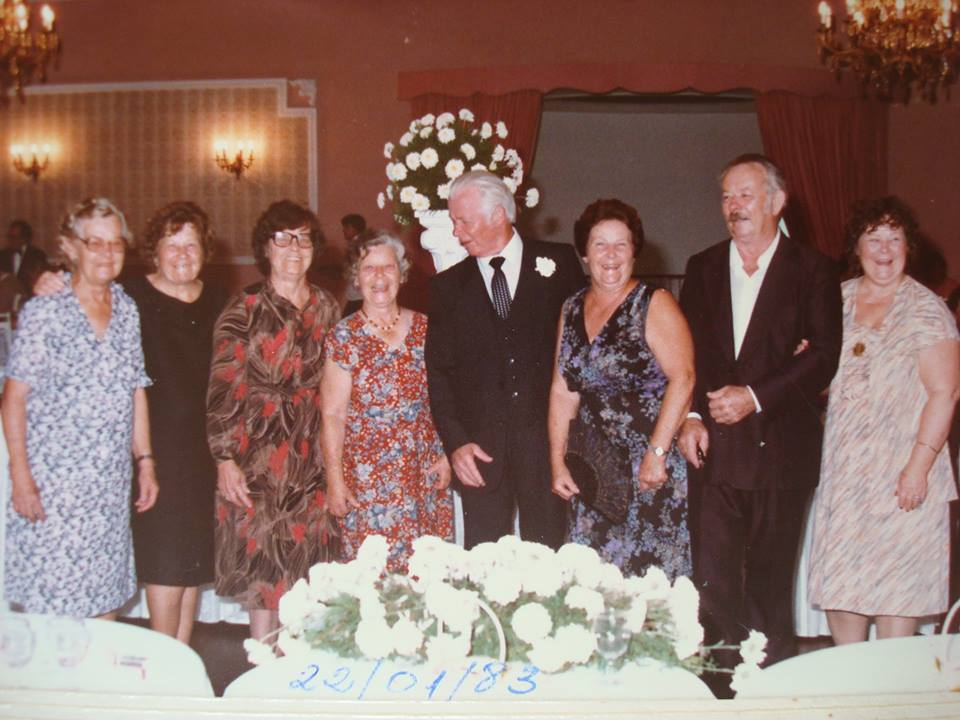
\includegraphics[width=0.85\linewidth,height=\textheight,keepaspectratio,alt={Oma Dora und ihre sieben Geschwister in einem Festsaal, am 22. Januar 1983 (Datum auf die Tischdecke geschrieben).}]{imagens/funke_oma_dora_7_irmaos_1983.jpg}
\caption{Oma Dora und ihre sieben Geschwister in einem Festsaal, am 22.
Januar 1983 (Datum auf die Tischdecke geschrieben).}
\end{figure}

Wenn ich die beiden Bilder nebeneinander betrachte, sehe ich etwas, das
die Genealogie selten zeigen kann: die Zeit, die an denselben Menschen
arbeitet. Die ernsten jungen Leute im Atelier, die mit der Feierlichkeit
von Menschen in die Kamera blicken, die nicht wissen, ob es je ein
zweites Foto geben wird, werden zu den lachenden Alten im Festsaal, die
keine Angst mehr vor der Kamera haben und sich umarmen, um ins Bild zu
passen. Zwischen dem einen Bild und dem anderen liegen ein Weltkrieg,
die Nationalisierungskampagne, die das Deutsche in den Schulen und auf
den Straßen verbot, und die Verwandlung Joinvilles von einer
Kolonistenstadt in eine Industriestadt. Dazwischen liegt auch das ganze
Leben von Dr.~Carlos Heinz, der im Januar 1983 dreiundvierzig Jahre alt
war und noch sechs vor sich hatte.

Pirabeiraba\index[lugares]{pirabeiraba@Pirabeiraba}, wo die Schule und die Gesundheitsstation mit seinem Namen
stehen, ist ein guter Ort, um Joinville\index[lugares]{joinville@Joinville} zu verstehen. Der Distrikt liegt
im Norden der Stadt, wo die Ebene auf das Gebirge trifft. Dort führt die
alte Estrada Dona Francisca vorbei, im 19. Jahrhundert angelegt, um die
Kolonie an der Küste mit der Hochebene von São Bento zu verbinden, eines
der Werke, auf die die Kolonisten am stolzesten waren. Es ist ein Land
der kleinen Höfe, der Bananen- und Reisfelder, der Kolonistenhäuser mit
gepflegten Gärten und auch der Flüsse, die eilig aus dem Gebirge
herabkommen und nach einem starken Regen leicht über die Ufer treten.
Ein Arzt, der dort arbeitete, behandelte Bauern, Arbeiter, die jeden Tag
zu den Fabriken der Stadt hinunterfuhren, Kinder mit Würmern, Alte mit
Bluthochdruck. Ich habe keine Liste der Orte, an denen Dr.~Carlos Heinz
praktizierte, und ich werde keine erfinden. Aber dass sein Name für zwei
Einrichtungen in diesem Distrikt gewählt wurde, sagt recht deutlich,
dass die Stadt ihn dort anerkannt hat.

Über ihren Vater schreibt Bárbara wenig, und ich respektiere dieses Maß.

\emph{Es ist seltsam, den Namen des eigenen Vaters auf einem Schild zu
sehen. Man wächst auf und nennt einen Menschen Papa, der für die anderen
der Doktor war. Nachdem er gestorben war (ich war damals ein Teenager),
ging sein Name an eine Schule und an eine Gesundheitsstation und gehörte
nicht mehr nur uns. Heute denke ich, dass auch das eine Art Erbe ist: zu
wissen, dass die Arbeit eines Menschen weiter genützt hat, nachdem er
gegangen war, an Orten, an denen keiner von uns war.}

Dr.~Carlos Heinz wäre übrigens um ein Haar im Deutschland Hitlers
geboren worden. Die Geschichte wird in Bárbaras Familie erzählt, und ich
halte sie so fest, wie sie mich erreicht hat.

\section{Der Weinkeller von 1939}\label{der-weinkeller-von-1939}

\emph{Sachsen\index[lugares]{sachsen@Sachsen} und Joinville\index[lugares]{joinville@Joinville}, 1939}

Im Jahr 1939 reisten Oscar Martin Funke\index[pessoas]{funke, oscar martin@Funke, Oscar Martin} und seine Frau, die Oma Dora\index[pessoas]{aenishaenslin, dora marta@Aenishaenslin, Dora Marta},
nach Deutschland. Oscar war 1910 in Glauchau\index[lugares]{glauchau@Glauchau} in Sachsen\index[lugares]{sachsen@Sachsen} geboren und als
Junge nach Joinville\index[lugares]{joinville@Joinville} gekommen; er war immer noch Deutscher. Dora war
Brasilianerin, 1914 in Joinville\index[lugares]{joinville@Joinville} geboren, und Bárbaras Familie bewahrt
über sie einen Satz, den ich nicht verbessern will: Sie hatte die
schönsten Beine von Blumenau\index[lugares]{blumenau@Blumenau}. In jenem Jahr war sie mit ihrem ersten
Kind schwanger.

Im Haus der Verwandten lud jemand Oscar ein, mit ihm in den Keller zu
gehen und einen Wein auszusuchen. Der Wein war der Vorwand. Unten, wo
niemand mithörte, sagte der Verwandte, was man in der Stube nicht laut
sagen durfte: Hitler sei schrecklich, der Krieg komme, und sie müssten
versuchen, sofort nach Brasilien zurückzukehren. Ein Mann von
neunundzwanzig Jahren, Deutscher, im wehrpflichtigen Alter, wäre
eingezogen worden, wenn er geblieben wäre.

Die Rückkehr war nicht einfach. Damit Oscar Deutschland verlassen
konnte, brauchte es die Hilfe des brasilianischen Konsuls, der ihm eine
Genehmigung ausstellte. Und im Hafen wurde um die Plätze auf dem Schiff
gestritten, in einer Zeit, in der viele weg wollten. Nach der
Überlieferung der Familie war es der Charme der Oma Dora\index[pessoas]{aenishaenslin, dora marta@Aenishaenslin, Dora Marta}, der die Sache
entschied. Schwanger, schön und Brasilianerin, bekam sie die Plätze.

Carlos Heinz Funke\index[pessoas]{funke, carlos heinz@Funke, Carlos Heinz} kam am 10. August 1939 in Joinville\index[lugares]{joinville@Joinville} zur Welt. Drei
Wochen später, am 1. September, überfiel Deutschland Polen, und der
Zweite Weltkrieg begann. Wäre der Verwandte nicht in den Weinkeller
gegangen, hätte der Konsul nein gesagt, hätte die Oma Dora\index[pessoas]{aenishaenslin, dora marta@Aenishaenslin, Dora Marta} am Kai
niemanden überzeugt, dann wäre der Schwiegervater, den ich nie
kennengelernt habe, im Sachsen\index[lugares]{sachsen@Sachsen} des Krieges geboren worden, als Sohn
eines Soldaten.

Ich kann diese Geschichte nicht lesen, ohne an die andere Seite der
Familie zu denken. 1913 verließen der Fata\index[pessoas]{haas, johann@Haas, Johann} und die Mota\index[pessoas]{meier, maria@Meier, Maria} Deutschland ein
Jahr vor dem Ersten Weltkrieg, durch die Tür von Marseille\index[lugares]{marseille@Marseille}, als die
Auswanderung nach den Worten meines Vaters schon versperrt war. 1939
verließen die Funke Deutschland wenige Wochen vor dem Zweiten, mit der
Hilfe eines Konsuls. Und beide Familien bewahrten dasselbe Bild eines
Kellers, in dem man die Wahrheit sagen konnte: den Keller in Ituporanga\index[lugares]{ituporanga@Ituporanga},
in dem der Fata\index[pessoas]{haas, johann@Haas, Johann} während des Krieges Radio hörte (Kapitel 7), und den
Weinkeller in Sachsen\index[lugares]{sachsen@Sachsen}, in dem ein Verwandter sagte, es sei Zeit zu
gehen.

\section{Der Lehrer von Nova
Petrópolis}\label{der-lehrer-von-nova-petruxf3polis}

Von der Seite von Bárbaras Mutter ist das älteste Foto, das ich habe,
das einer Schule. Auch dieses ist eine Reproduktion: ein kleines
Schwarzweißfoto, auf einen rosafarbenen Stoff gelegt und von oben
fotografiert. Darauf stehen etwa vierzig Schüler in Reihen vor einem
Gebäude, die vorderen in der Hocke, die hinteren stehend, fast alle in
weißem Hemd oder weißer Bluse, die Mädchen mit dunklem Rock. In der
Mitte, im dunklen Anzug, ein erwachsener Mann. Dahinter etwas, das wie
eine Fahne aussieht. Es ist Opa Erno\index[pessoas]{hoeveler, erno@Hoeveler, Erno} Hoeveler, euer Urgroßvater, Lehrer.

\begin{figure}
\centering
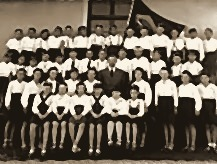
\includegraphics[width=0.85\linewidth,height=\textheight,keepaspectratio,alt={Der Urgroßvater Erno Hoeveler („Opa Erno``), lutherischer Lehrer an Gemeindeschulen in Rio Grande do Sul, umgeben von seinen Schülern. Reproduktion eines alten Fotos. Kontrast und Töne korrigiert.}]{imagens/hoeveler_vo_erno_escola_restaurada.jpg}
\caption{Der Urgroßvater Erno Hoeveler („Opa Erno``), lutherischer
Lehrer an Gemeindeschulen in Rio Grande do Sul, umgeben von seinen
Schülern. Reproduktion eines alten Fotos. Kontrast und Töne korrigiert.}
\end{figure}

Erno Hoeveler\index[pessoas]{hoeveler, erno@Hoeveler, Erno} war Lehrer an Schulen der evangelischen Gemeinde in
Estrela\index[lugares]{estrela@Estrela} und in Nova Petrópolis\index[lugares]{nova petropolis@Nova Petrópolis}, in Rio Grande do Sul. Er heiratete
Rosita Érica Lohmann\index[pessoas]{lohmann, rosita erica@Lohmann, Rosita Érica}, die Tochter von Francisco Jacob Lohmann\index[pessoas]{lohmann, francisco jacob@Lohmann, Francisco Jacob} und
Miguelina Endres\index[pessoas]{endres, miguelina leocadia@Endres, Miguelina Leocádia}, und hatte mit ihr vier Kinder, darunter Ilusca und
Walter. In den deutschen Kolonien des Südens war der Lehrer der
Gemeindeschule eine zentrale Gestalt, oft neben dem Pastor der einzige
gebildete Mann am Ort. Er brachte das Lesen auf Deutsch und auf
Portugiesisch bei, lehrte Rechnen und Katechismus und leitete häufig den
Chor und half beim Gottesdienst. Reich wurde man mit diesem Beruf nicht.
Ilusca selbst sagte das ganz schlicht in einer Zeitungsreportage über
die Weihnachten von früher in Joinville\index[lugares]{joinville@Joinville}: Der Vater war Lehrer und
verdiente wenig, und deshalb wurden viele Weihnachtsgeschenke repariert
und wiederverwendet, und manchmal bestand das Geschenk aus Äpfeln und
Keksen.

In derselben Reportage erzählt sie von zwei Geschenken, die ihre
Kindheit geprägt haben. Eine Puppe, die sie bis heute aufbewahrt, mit
Augen, die die Zeit schon eingesunken hat, und eine gebrauchte Geige,
die der Vater in einem Pfandhaus in Porto Alegre gekauft hatte. Ich lese
diesen Satz und sehe Opa Erno\index[pessoas]{hoeveler, erno@Hoeveler, Erno}, den ich auch nicht gekannt habe, mit dem
knappen Gehalt eines Kolonielehrers ein Pfandhaus in der Hauptstadt
betreten, zwischen Dingen wählen, die andere Familien aus Not
zurückgelassen hatten, und mit einer Geige für die Tochter wieder
herauskommen. Ich kenne weder das Jahr noch den Laden, und ich muss sie
nicht kennen. Als Ilusca heiratete, so erzählte sie, schenkte sie die
Geige einem Neffen.

Ilusca, die Tochter des Lehrers, der wenig verdiente, wurde
Rechtsanwältin. Für eine junge Frau, die um 1943 in einer
Kolonistenfamilie geboren war, Tochter eines Gemeindeschullehrers, war
das ein Generationensprung, so groß wie der von Johann Haas\index[pessoas]{haas, johann@Haas, Johann}, als er
Bayern\index[lugares]{bayern@Bayern} gegen Rio do Ouro\index[lugares]{rio do ouro@Rio do Ouro} eintauschte. In zwei Generationen hatte die
Familie, die vom knappen Gehalt eines Schulmeisters lebte, in ein und
demselben Haus in Joinville\index[lugares]{joinville@Joinville} eine Anwältin und einen Arzt. Ich verkläre
diesen Sprung nicht. Ich stelle mir vor, dass er Jahre des Lernens
gekostet hat, Entfernung von zu Hause und etwas Einsamkeit, wie er alle
Kolonistenkinder gekostet hat, die als Erste ihrer Familie an eine
Hochschule kamen. Aber er ist geschehen, und er wurde aus demselben
Stoff gemacht wie die Geige aus dem Pfandhaus: aus der Überzeugung, dass
es sich lohnte, für das Geld auszugeben, was einen Menschen bildet.

Die Tradition des Lehrens scheint auf dieser Seite der Familie tief zu
reichen. In Kapitel 12 werdet ihr lesen, dass der erste Lohmann, der
1846 nach Rio Grande do Sul kam, der Sohn eines Lehrers war und dass der
Lohmann-Familienverband in Deutschland stolz darauf war, seit dem 17.
Jahrhundert Schulmeister und Pastoren „in allen Verzweigungen`` gehabt
zu haben. Erno war ein Hoeveler, kein Lohmann, und er heiratete in die
Familie ein, statt in sie hineingeboren zu werden. Trotzdem fällt es
schwer, darin kein Muster zu sehen. Die Lohmann hatten eine Tradition
von Lehrern und verheirateten eine Tochter mit einem Lehrer.

Der lutherische Glaube war der andere Faden. Hier spricht wieder
Bárbara.

\emph{Kathe hat das einer Zeitung in Joinville\index[lugares]{joinville@Joinville} besser erzählt, als ich
es könnte: Weihnachten kam, wenn die Oma anfing, Plätzchen zu backen.
Die Ausstechformen, sagte meine Mutter im selben Interview, sind noch
dieselben. Den Advent nahm man ernst, mit dem Kranz mit vier Kerzen, an
jedem Sonntag eine mehr angezündet, und mit den Liedern aus dem
Gesangbuch. Am Abend des 24. ging meine Mutter als Erste ins Wohnzimmer
und zündete die Kerzen an, und die anderen kamen danach singend herein.
In der Krippe blieb die Wiege bis zum Weihnachtstag leer, weil das
Christkind erst kam, wenn es geboren wurde.}

\emph{Als mein Vater starb, musste jemand an Heiligabend seinen Platz
einnehmen und die Andacht und die Lieder anstimmen. Das war unser
Bruder, der Pianist der Familie. Ich glaube, das ist ein Erbe, so
greifbar wie ein Haus: der Platz an der Spitze der Familie am Abend des
24., der von einem zum anderen übergeht, wenn jemand fehlt.}

Für den Forscher in mir liegt der Wert dieses Abschnitts darin, dass er
nicht nur vom Gedächtnis eines einzigen Menschen abhängt. Die in
Joinville\index[lugares]{joinville@Joinville} veröffentlichte Reportage bringt die Aussagen von Katherine
und von Ilusca, und beide beschreiben dasselbe Haus und dieselben
Bräuche. Die Oma mit den Plätzchen, die Adventskerzen und die leere
Wiege sind dokumentiert.

Aus Nova Petrópolis\index[lugares]{nova petropolis@Nova Petrópolis} kam auch der Onkel, der einem Buch seinen Namen gab.
Walter Hoeveler\index[pessoas]{hoeveler, walter@Hoeveler, Walter}, Iluscas Bruder, in der Familie Onkel Walter, zog 1960
nach Florianópolis\index[lugares]{florianopolis@Florianópolis}. Katherine Funke, Journalistin und Schriftstellerin,
Bárbaras Schwester, veröffentlichte 2013 \emph{Viagens de Walter}
(„Walters Reisen``), von ihm inspiriert. Ich denke gern, dass in dieser
Familie außer gelehrt auch geschrieben wird. Katherine schrieb über den
Onkel, Bárbara schreibt hier mit mir, und ich schreibe für euch.

\section{Die Kiste mit den Bildern}\label{die-kiste-mit-den-bildern}

Oma Rosita\index[pessoas]{lohmann, rosita erica@Lohmann, Rosita Érica} starb 2014 in Joinville\index[lugares]{joinville@Joinville}, mit über neunzig Jahren. Die
Reportage über die Weihnachtsfeste erschien ein Jahr später, und darin
erzählt die Familie, dass am ersten Weihnachtsfest ohne sie der echte
Weihnachtsbaum durch einen künstlichen mit Lichterkette ersetzt wurde.
Ilusca erklärte den Wechsel mit einer einfachen Rechnung: Früher waren
es sechs Leute, die den Baum aufstellten, und jetzt war nur noch sie da.
In der ganzen Reportage ist das der Satz, der mich am meisten berührt:
Er spricht von Arbeitskraft. So zeigen sich Verluste in einer Familie:
Jemand fehlt, und eine Aufgabe, die vielen gehörte, gehört nur noch
einem.

Nach Rositas Tod blieben ihre Sachen zurück, darunter die Bilder. Ich
weiß nicht, ob sie alle in einer Kiste lagen, wie man es in Geschichten
sagt, oder verteilt in Alben und Schubladen. Ich weiß, dass eines
darunter war, das für diese Nachforschung mehr wert war als alle
anderen.

Es ist ein Hochzeitsbild in einem Rahmen aus erdfarbenem Karton mit
einer Zierleiste aus feinen Linien. Es ist nicht oval, wie ich es in
Erinnerung hatte und wie ich es sogar im Entwurf des Konzepts für dieses
Buch geschrieben hatte: Die Erinnerung rundet die Dinge ab. Die Braut
steht links, mit einem langen Schleier, der von einem Blumenkranz
gehalten wird, einem weißen Kleid mit hohem Kragen und langen Ärmeln und
einem ernsten, runden Gesicht. Der Bräutigam steht rechts, im dunklen
Anzug mit Weste, weißer Fliege, einem Blumensträußchen am Revers und
einer Uhrkette, die an der Weste zu sehen ist. Er hat einen Schnurrbart,
kurzes, zur Seite gekämmtes Haar, und die Hand der Braut ruht auf seinem
Arm. Hinter ihnen die gemalte Kulisse eines Fotoateliers, mit einem
falschen Fenster und gezeichnetem Blattwerk. Es sind Francisco Jacob
Lohmann und Miguelina Leocádia Endres\index[pessoas]{endres, miguelina leocadia@Endres, Miguelina Leocádia}, bei ihrer Hochzeit am 5.
September 1914. Bárbaras Urgroßeltern. Eure Ururgroßeltern.

\begin{figure}
\centering
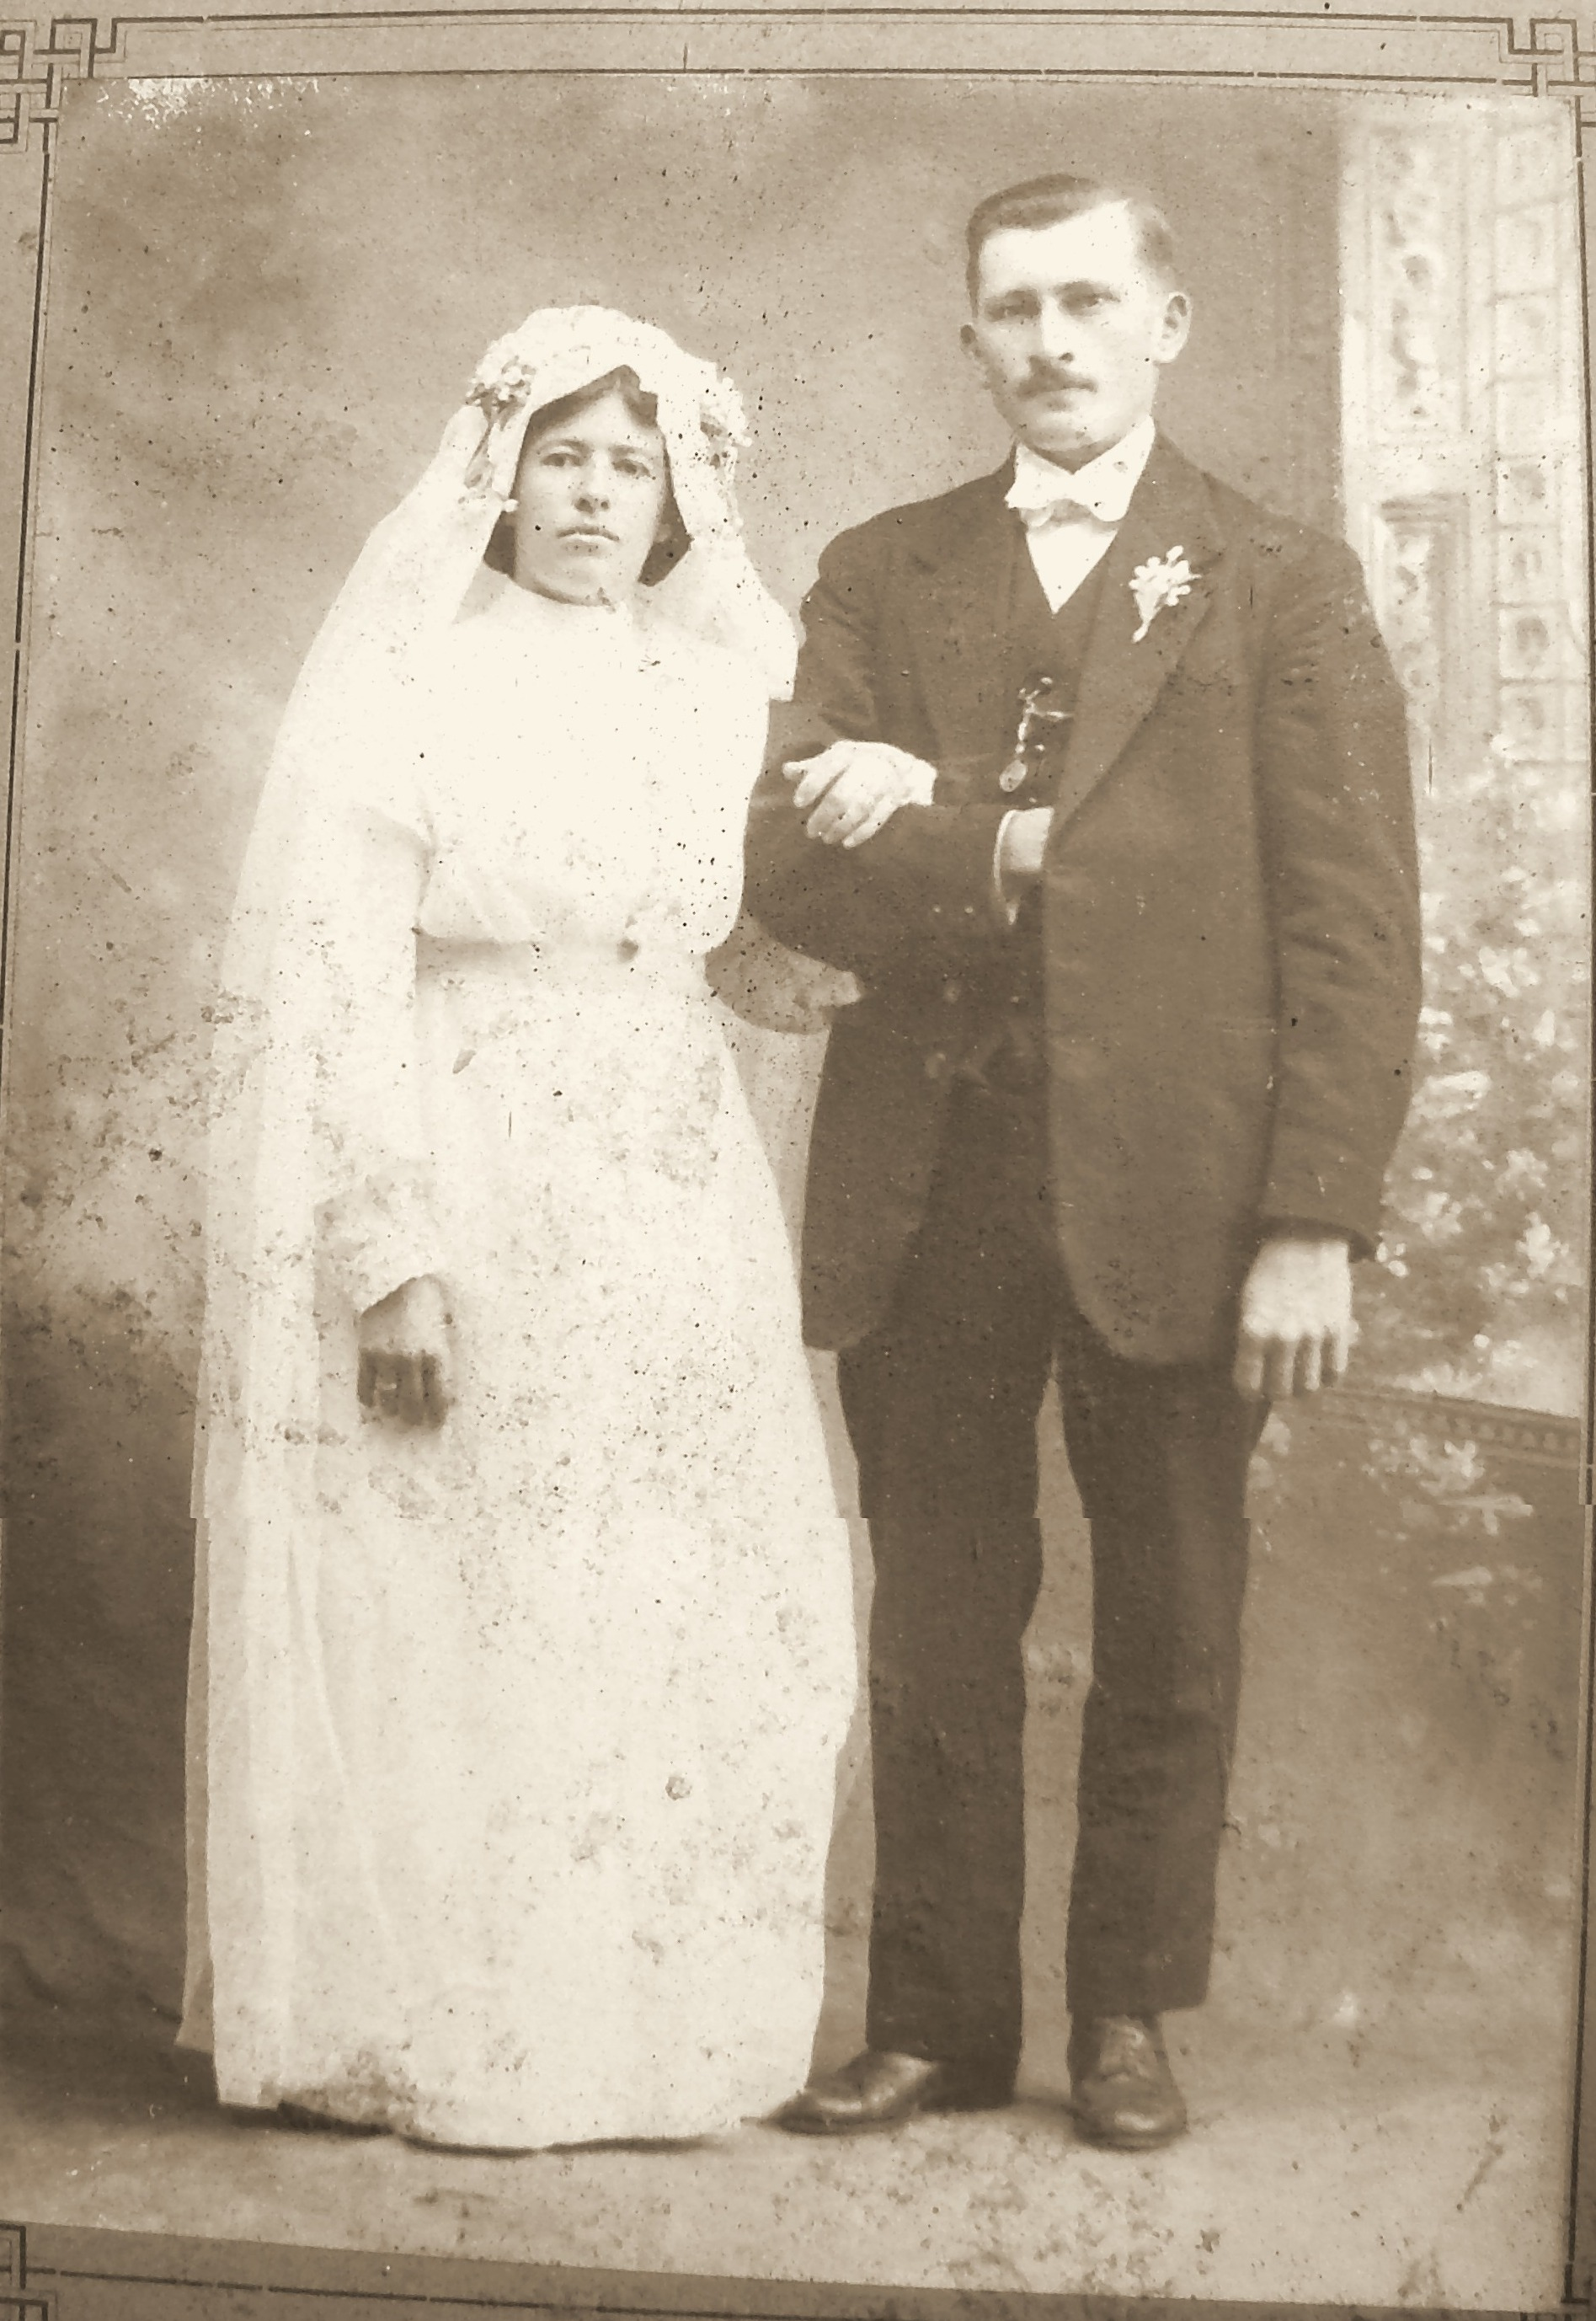
\includegraphics[width=0.85\linewidth,height=\textheight,keepaspectratio,alt={Hochzeitsbild von Francisco Jacob Lohmann (1889--1975) und Miguelina Leocádia Endres (geb. 1891) vom 5. September 1914, aufbewahrt von Oma Rosita: Bárbaras Urgroßeltern und die Ururgroßeltern von Matheus und Lucas. Kontrast und Töne korrigiert.}]{imagens/lohmann_bisavo_francisco_e_bisavo_michelina_restaurada.jpg}
\caption{Hochzeitsbild von Francisco Jacob Lohmann (1889--1975) und
Miguelina Leocádia Endres\index[pessoas]{endres, miguelina leocadia@Endres, Miguelina Leocádia} (geb. 1891) vom 5. September 1914, aufbewahrt
von Oma Rosita\index[pessoas]{lohmann, rosita erica@Lohmann, Rosita Érica}: Bárbaras Urgroßeltern und die Ururgroßeltern von Matheus
und Lucas. Kontrast und Töne korrigiert.}
\end{figure}

Aus Gewohnheit rechne ich nach. Francisco wurde am 20. November 1889
geboren, war also am Tag des Bildes vierundzwanzig Jahre alt. Miguelina,
geboren am 9. Dezember 1891, war zweiundzwanzig. Auf der anderen Seite
des Ozeans hatte einen Monat zuvor der Erste Weltkrieg begonnen. In
Santa Catarina waren die Haas seit anderthalb Jahren in Brasilien und
hatten Luisa\index[pessoas]{haas, luisa@Haas, Luisa} und Walter begraben. Nichts davon ist auf dem Bild zu
sehen, und vielleicht ist nichts davon bis in jenes Atelier im Vale do
Taquari gedrungen, wo ein junger Mann, der seine Mutter nie gekannt
hatte, mit Schnurrbart und Fliege posierte, um seine eigene Familie zu
gründen.

Dieser junge Mann, der seine Mutter nie gekannt hatte, ist die Spur, die
mich zum nächsten Kapitel geführt hat. Als ich den Stammbaum bei
FamilySearch aufbaute, brachte das Profil von Francisco Jacob ein Datum,
das mich innehalten ließ: Seine Mutter, Suzana Regina Schnack\index[pessoas]{schnack, suzana regina@Schnack, Suzana Regina}, starb am
16. Dezember 1889, sechsundzwanzig Tage nach seiner Geburt. Dieser Mann
wuchs ohne Mutter auf und sollte mit der jungen Frau mit dem Schleier
auf dem Bild zwölf Kinder haben. Eine der Töchter war Rosita, die das
Bild ihr Leben lang aufbewahrte und es der Enkelin hinterließ.

Ich schließe dieses Kapitel mit Bárbara.

\emph{Ich hatte dieses Bild schon oft gesehen, ohne es wirklich
anzuschauen. Es war das Foto der Urgroßeltern, mehr nicht. Erst als
Reinaldo anfing, den Stammbaum aufzubauen, und wir uns mit den Daten vor
uns hinsetzten, verstand ich, dass der junge Mann mit dem Schnurrbart
seine Mutter verloren hatte, als er noch keinen Monat alt war. Ich
dachte an die Frau, die ihn großgezogen hat, an das Haus, in dem er
aufwuchs, und daran, was es für einen solchen Mann bedeutet, zwölf
Kinder zu haben. Ich weiß nicht, ob Oma Rosita\index[pessoas]{lohmann, rosita erica@Lohmann, Rosita Érica} diese Geschichte im
Einzelnen kannte. Wenn ja, fand sie vielleicht, dass man so etwas nicht
erzählt.}

\emph{Da beschlossen wir hinzufahren. Wenn die Oma nicht mehr da war, um
zu erzählen, so waren ihre Geschwister noch da. Im September 2012 fuhren
wir mit den Jungen nach Rio Grande.}

In der Ordnung des Buches erzähle ich diese Reise jetzt, nach Rositas
Tod. In der Ordnung des Lebens fand sie früher statt, im September 2012,
als Oma Rosita\index[pessoas]{lohmann, rosita erica@Lohmann, Rosita Érica} noch in Joinville\index[lugares]{joinville@Joinville} lebte und vier ihrer Geschwister im
Vale do Taquari auf uns warteten. Um zu verstehen, wer Francisco und
Miguelina auf dem Hochzeitsbild waren, mussten wir dorthin, das Gebirge
hinunter.

\section{Für euch zum Entdecken}\label{fuxfcr-euch-zum-entdecken-10}

\begin{itemize}
\tightlist
\item
  Wann und warum kamen die Funke aus Glauchau\index[lugares]{glauchau@Glauchau} nach Joinville\index[lugares]{joinville@Joinville}? Sind sich
  die Funke und die Haas vor 1913 in Sachsen\index[lugares]{sachsen@Sachsen} begegnet?
\item
  Wer ist die junge Frau im blauen Kleid auf dem Foto aus der Garage?
  Fragt eure Mutter und eure Tanten.
\item
  Auf dem alten Bild der Familie von Oma Dora\index[pessoas]{aenishaenslin, dora marta@Aenishaenslin, Dora Marta} habe ich neun Kinder
  gezählt; beim Fest am 22. Januar 1983 sind Dora und sieben weitere zu
  sehen. Fehlte eines der Geschwister, oder habe ich mich verzählt?
  Bárbara und ihre Schwestern sind die Ersten, die ihr fragen solltet.
\item
  Wer ging 1939 mit Oscar in den Weinkeller, und in welcher Stadt? War
  es Glauchau\index[lugares]{glauchau@Glauchau}, wo er geboren wurde? Mit welchem Schiff kehrte das Paar
  zurück, und was stand in der Genehmigung des brasilianischen Konsuls?
  Fragt in Bárbaras Familie, ob jemand den Reisepass oder die
  Schiffskarte aufbewahrt hat.
\item
  Wo und wie haben sich Carlos Heinz Funke\index[pessoas]{funke, carlos heinz@Funke, Carlos Heinz} und Ilusca kennengelernt? Das
  Universitätsleben in Porto Alegre ist nur eine Hypothese von mir.
\item
  Wer ist der Neffe, der die Geige aus dem Pfandhaus bekam, als Ilusca
  heiratete, und wo ist diese Geige heute?
\end{itemize}

\chapter{Von der Fazenda Lohmann zu den Friedhöfen von Estrela --- Das
Taquari-Tal}\label{cap-12}

\begin{quote}
\emph{Die Flüsse des Südens haben ein langes Gedächtnis. Wer an ihren
Ufern wohnt, braucht auch eines.}
\end{quote}

\emph{29,3° S · 51,9° W, Palmas\index[lugares]{palmas@Palmas}, Arroio do Meio\index[lugares]{arroio do meio@Arroio do Meio}, RS}

Die Familie sagt, Francisco Jacob Lohmann\index[pessoas]{lohmann, francisco jacob@Lohmann, Francisco Jacob} und Miguelina Leocádia Endres\index[pessoas]{endres, miguelina leocadia@Endres, Miguelina Leocádia}
hätten zwölf Kinder gehabt. Die Register geben zweien von ihnen
Geburtsdaten, die vor der Hochzeit der Eltern liegen, und führen zwei
Walter. Auf der Fotografie vor dem neuen Haus habe ich elf gezählt.

\section{September 2012}\label{september-2012}

\emph{Arroio do Meio\index[lugares]{arroio do meio@Arroio do Meio} und Estrela\index[lugares]{estrela@Estrela}, Rio Grande do Sul, 25. September 2012}

Wir kamen im Frühling ins Taquari-Tal. Die Hügel waren tiefgrün, und der
Fluss zog breit zwischen ihnen dahin. Matheus war zehn, Lucas sieben.
Wir hatten eine Liste mit Namen dabei. Das Ziel der Reise war leicht zu
sagen und schwer zu erfüllen: die Geschwister von Oma Rosita\index[pessoas]{lohmann, rosita erica@Lohmann, Rosita Érica} zu finden,
solange sie noch lebten.

Von den zwölf Kindern von Francisco Jacob Lohmann\index[pessoas]{lohmann, francisco jacob@Lohmann, Francisco Jacob} und Miguelina Leocádia
Endres lebten 2012 noch einige, verstreut über Arroio do Meio\index[lugares]{arroio do meio@Arroio do Meio}, Estrela\index[lugares]{estrela@Estrela}
und die Umgebung, in Kolonistenhäusern und Kleinstadthäusern. Nach den
Daten, die FamilySearch uns liefert, war Onkel Urbano etwa
achtundneunzig Jahre alt, Onkel Armando etwa sechsundneunzig, Tante
Sunta etwa einundneunzig und der Jüngste, Onkel Arlindo, achtundachtzig.
Sie waren die letzte Generation, die Francisco und Miguelina mit eigenen
Augen gesehen hatte.

Die Gespräche jener Tage werde ich hier nicht nachzeichnen. Ich habe sie
nicht aufgenommen, so wie ich meine Mutter bei der Eisernen Hochzeit
aufgenommen habe, und meine Erinnerung daran ist die eines bewegten
Besuchers, nicht die eines Protokollführers. Es wäre leicht, den Onkeln
und Tanten schöne Sätze über das Hochwasser von 1941, über den
verwitweten Vater oder über das neue Haus in den Mund zu legen. Das tue
ich nicht. Was ich tun kann: die Fotografien beschreiben, die über das,
was sie zeigen, nicht lügen, und sagen, was ich empfunden habe.

Der Besuch bei Onkel Armando fand auf der Veranda eines Kolonistenhofs
statt. Auf dem Foto sitzt er auf einem niedrigen Stuhl, in einem dunklen
Wollpullover, das weiße Haar zerzaust, mit dem schiefen Lächeln eines
Mannes, den etwas belustigt, das außerhalb des Bildes geblieben ist. Ich
sitze neben ihm, in einer Jacke, den Arm um seine Schultern gelegt. Die
Bildunterschrift der Familie sagt, dass Bárbara bei diesem Besuch dabei
war. Im Hintergrund eine gemauerte Säule mit abblätterndem Putz, eine
alte Satellitenschüssel, ein Backsteinschuppen, die Weide und der
bewaldete Hügel. Der Himmel ist weiß. Es ist die Landschaft fast aller
deutschen Kolonien im Süden, und ich erkannte sie wieder, als wäre es
die von Vidal Ramos\index[lugares]{vidal ramos@Vidal Ramos}.

\begin{figure}
\centering
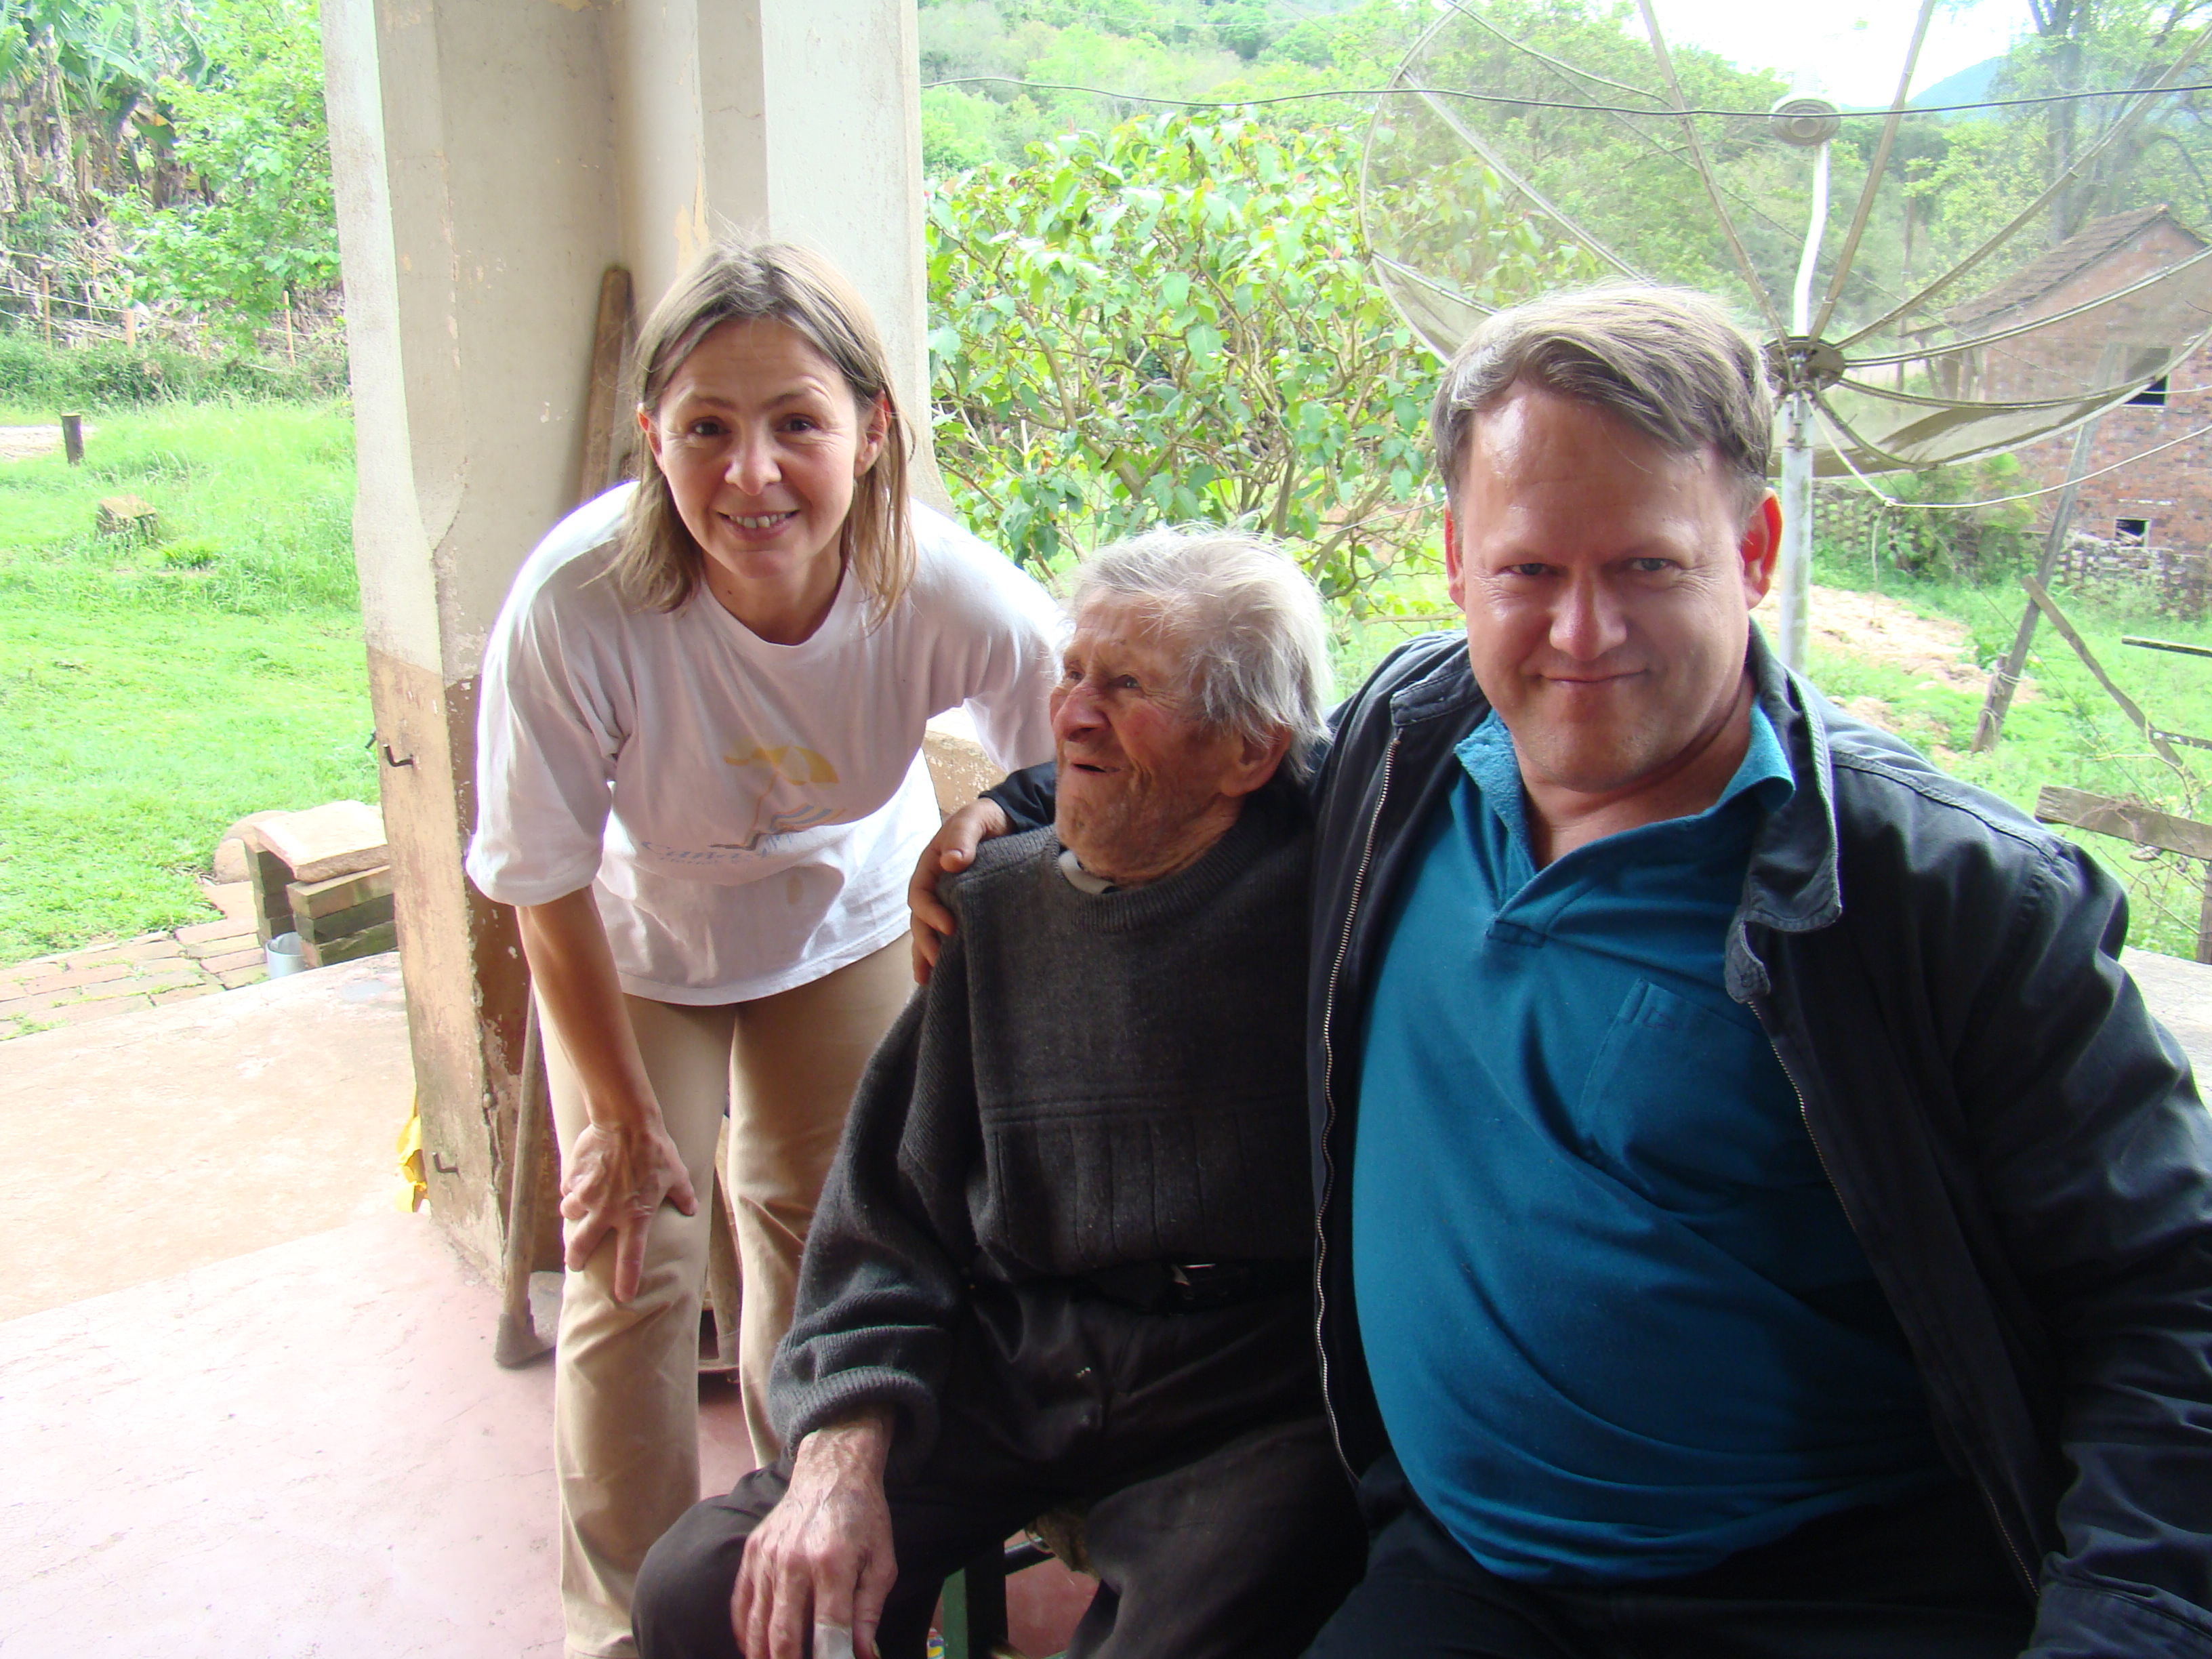
\includegraphics[width=0.85\linewidth,height=\textheight,keepaspectratio,alt={Besuch bei Onkel Armando Ernesto Lohmann (geb. 1916), einem Bruder von Oma Rosita, auf der Veranda seines Hauses im Taquari-Tal, September 2012.}]{imagens/lohmann_visita_tio_armando_2012.jpg}
\caption{Besuch bei Onkel Armando Ernesto Lohmann (geb. 1916), einem
Bruder von Oma Rosita\index[pessoas]{lohmann, rosita erica@Lohmann, Rosita Érica}, auf der Veranda seines Hauses im Taquari-Tal,
September 2012.}
\end{figure}

Im Haus von Onkel Urbano, dem ältesten der Geschwister, die wir trafen,
zeigt das Foto eine gelbe Veranda mit einem Topf Orchideen im
Hintergrund. Er sitzt in der Mitte, in einem gemusterten Pullover und
einer Anzughose, die großen Hände im Schoß gefaltet, mit dem festen
Blick eines Mannes, der fast ein Jahrhundert gesehen hat. Neben ihm eine
Frau in einer lila Bluse. Ich stehe links, Matheus auf dem Arm, der mit
beiden Daumen nach oben zeigt, und Lucas im roten T-Shirt steht hinter
uns auf einem Strohstuhl, lacht und überragt alle. Dahinter stehen
weitere Verwandte aus dem Haus. Wie in der Garage in Joinville\index[lugares]{joinville@Joinville} verbindet
das Bild weit entfernte Enden derselben Linie: meine Söhne am jüngsten,
einen Urgroßonkel am ältesten.

\begin{figure}
\centering
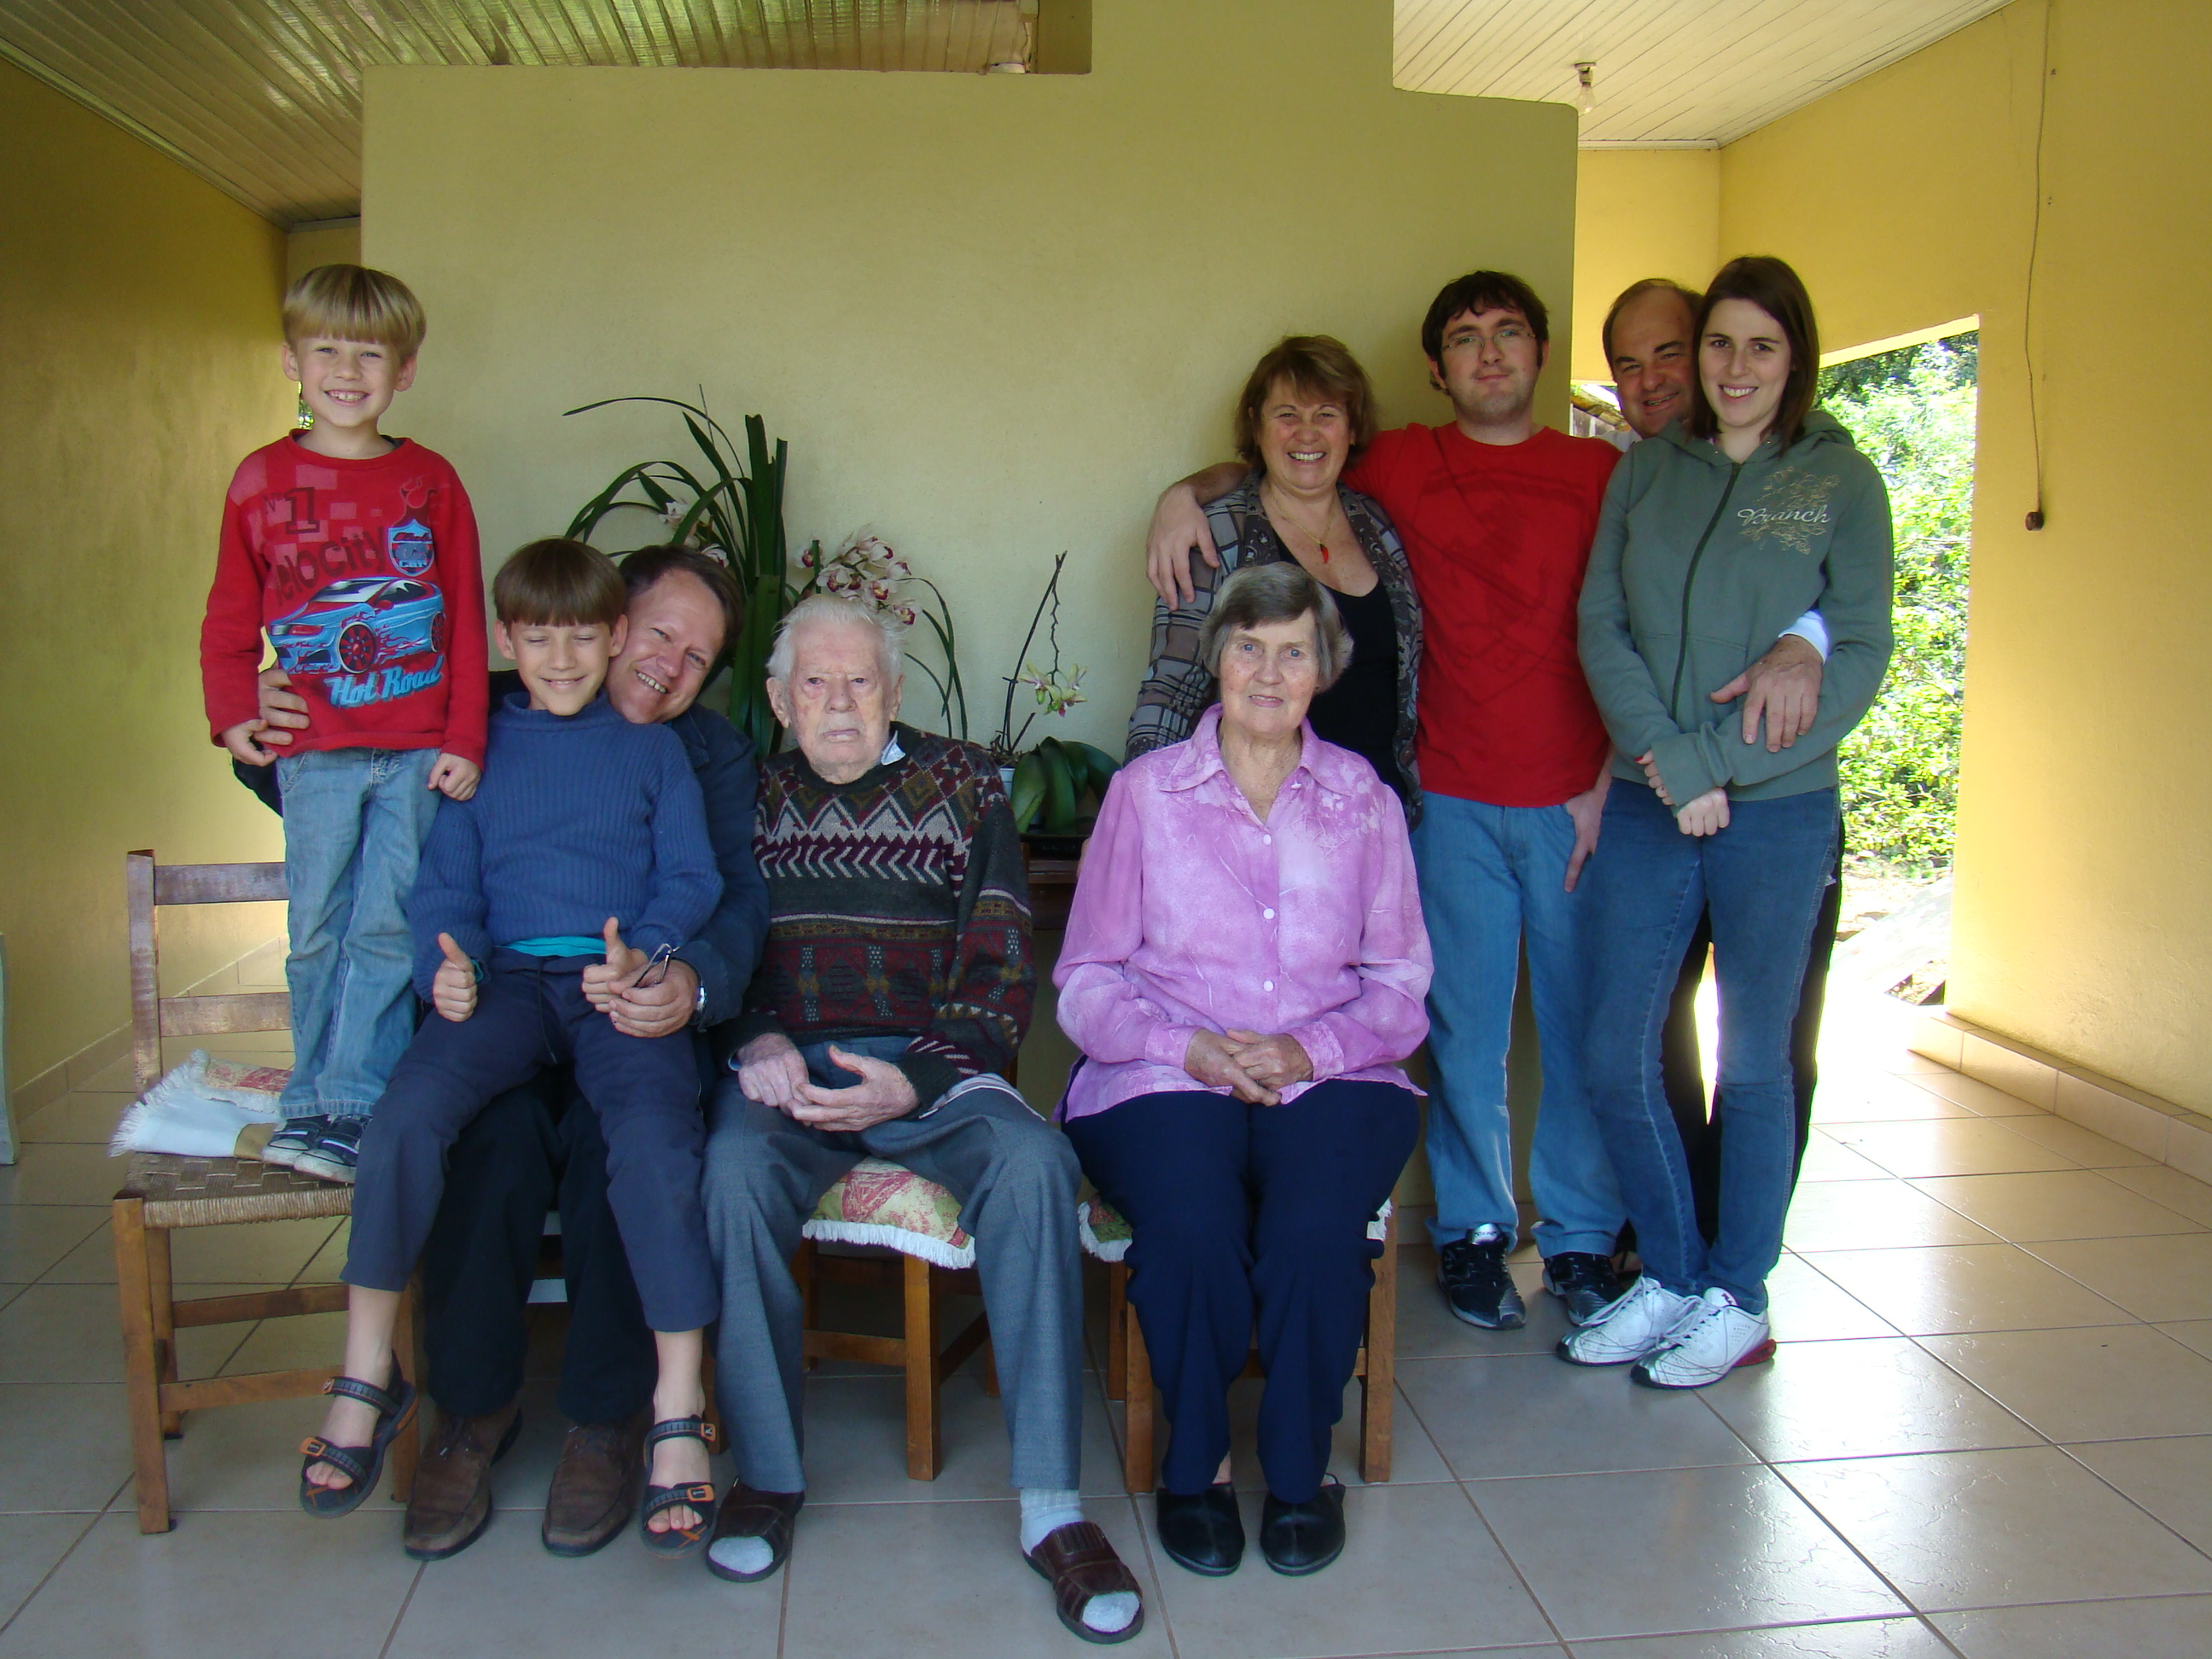
\includegraphics[width=0.85\linewidth,height=\textheight,keepaspectratio,alt={Besuch bei Onkel Urbano Aldo Lohmann (geb. 1914), dem ältesten der Geschwister von Oma Rosita, die die Familie im September 2012 antraf, mit Reinaldo, Matheus und Lucas und Verwandten aus dem Haus.}]{imagens/lohmann_visita_tio_urbano_2012.jpg}
\caption{Besuch bei Onkel Urbano Aldo Lohmann (geb. 1914), dem ältesten
der Geschwister von Oma Rosita\index[pessoas]{lohmann, rosita erica@Lohmann, Rosita Érica}, die die Familie im September 2012
antraf, mit Reinaldo, Matheus und Lucas und Verwandten aus dem Haus.}
\end{figure}

Der Besuch bei Onkel Arlindo war am Abend, in einem Zimmer mit
Spitzengardinen, einem Bild einer gelben Orchidee an der Wand und rotem
Teppichboden. Auf dem Foto, mit Blitz aufgenommen, stehen wir alle,
aneinandergelehnt wie auf einem Abschlussfoto, außer einer alten Dame,
die in der Ecke sitzen geblieben ist. Lucas steht genau in der Mitte, im
roten T-Shirt, Matheus im blauen Pullover links. Onkel Arlindo starb am
7. Februar 2018 in Estrela\index[lugares]{estrela@Estrela}, einen Tag nach seinem vierundneunzigsten
Geburtstag. Am Tag davor, dem 6. Februar, stand ich am Schalter des
\emph{Standesamts} Maxhütte-Haidhof\index[lugares]{maxhutte-haidhof@Maxhütte-Haidhof} in der Oberpfalz\index[lugares]{oberpfalz@Oberpfalz}, den Geburtseintrag
meines Großvaters in den Händen. Die beiden Daten sind in meinem
Kalender für immer verbunden.

\begin{figure}
\centering
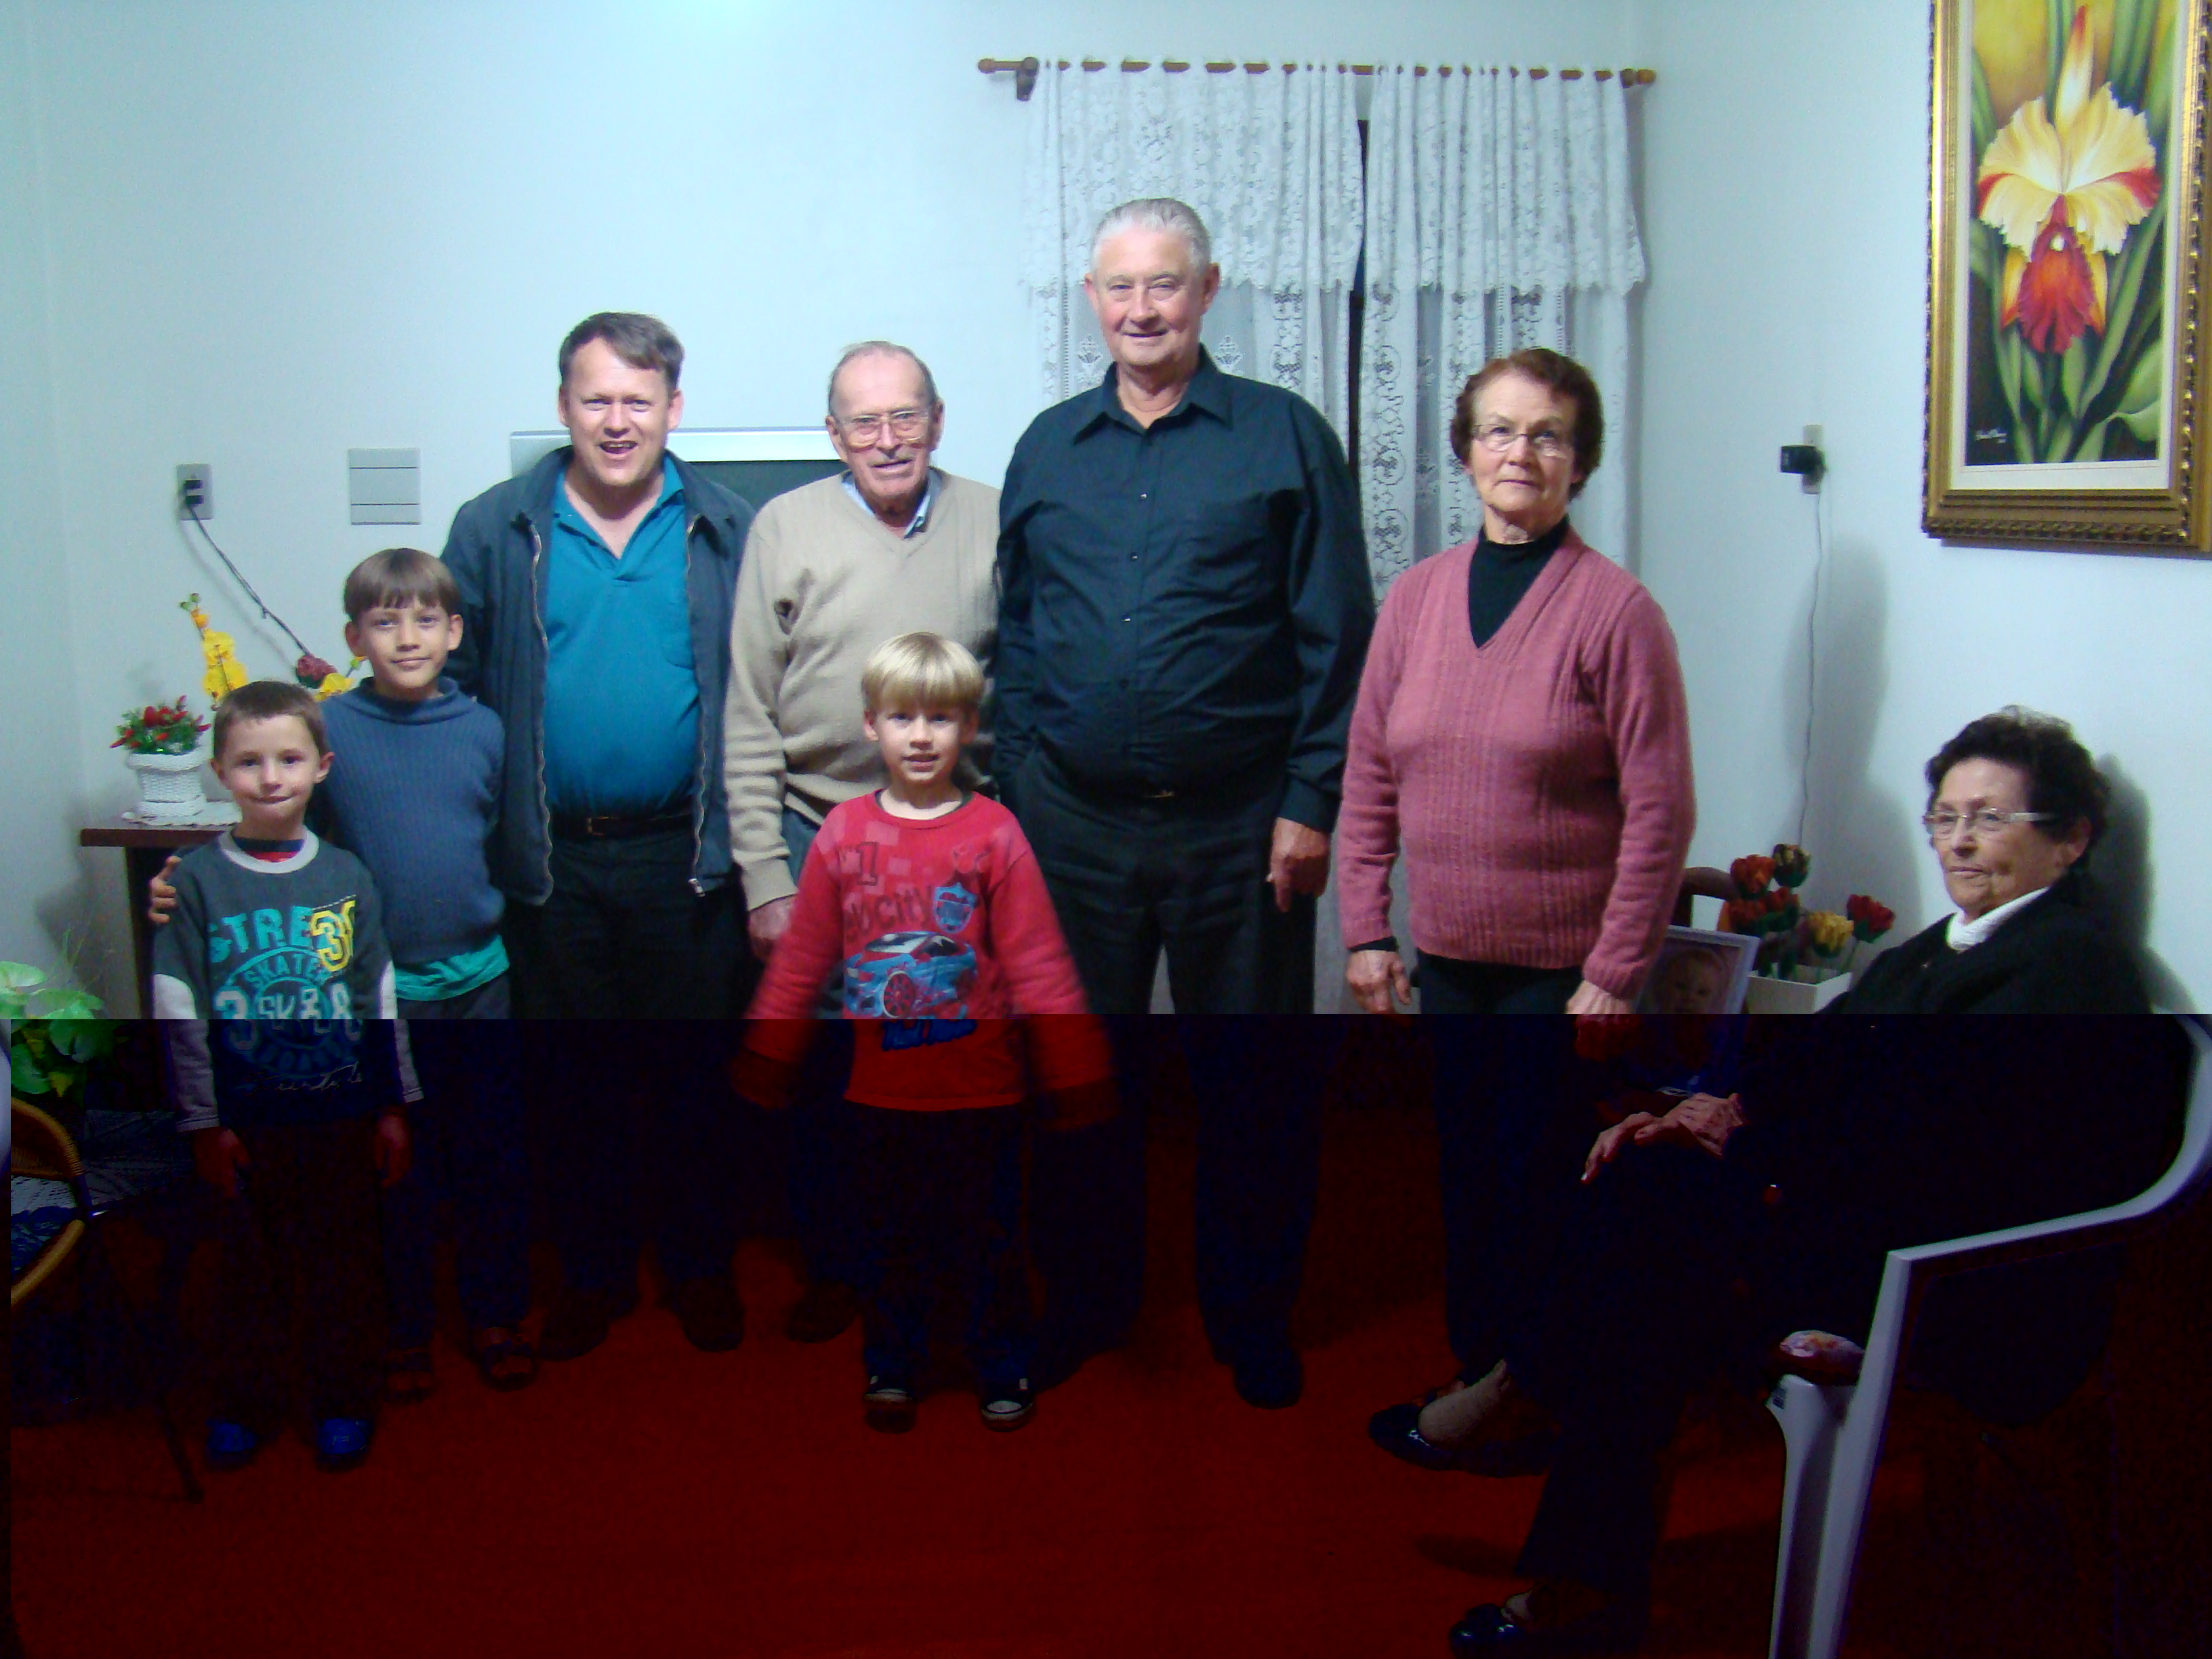
\includegraphics[width=0.85\linewidth,height=\textheight,keepaspectratio,alt={Besuch bei Onkel Arlindo Erno Lohmann (1924--2018), dem Jüngsten der zwölf Geschwister, im September 2012: Reinaldo, Matheus und Lucas mit dem Großonkel und Familienangehörigen.}]{imagens/lohmann_visita_tio_arlindo_2012.jpg}
\caption{Besuch bei Onkel Arlindo Erno Lohmann (1924--2018), dem
Jüngsten der zwölf Geschwister, im September 2012: Reinaldo, Matheus und
Lucas mit dem Großonkel und Familienangehörigen.}
\end{figure}

Das letzte Foto zeigt Tante Sunta, Asunda Erna Lohmann. Es ist mir das
liebste, wegen eines Details. Sie sitzt in einem abgewetzten Ledersessel
auf einem Kieshof vor einem orange gestrichenen Haus, die Hände
gefaltet, mit dem ernsten Gesicht eines Menschen, der sich nicht gern
fotografieren lässt. Um sie herum stehen und sitzen Verwandte aus dem
Haus und eine junge Frau mit einem Hündchen auf dem Schoß. Matheus und
Lucas stehen an der Tür, und die Bildunterschrift der Familie hält fest,
dass Bárbara sie bei diesem Besuch begleitete. Im Vordergrund stehen,
Tante Sunta zugewandt, vier leere Stühle: einer aus weißem Plastik, zwei
aus Holz, ein gestreifter Strandstuhl. Dort hatte das Gespräch
stattgefunden. Wer für das Foto aufgestanden war, hatte die Stühle so
stehen lassen, wie sie waren, ihr zugewandt.

\begin{figure}
\centering
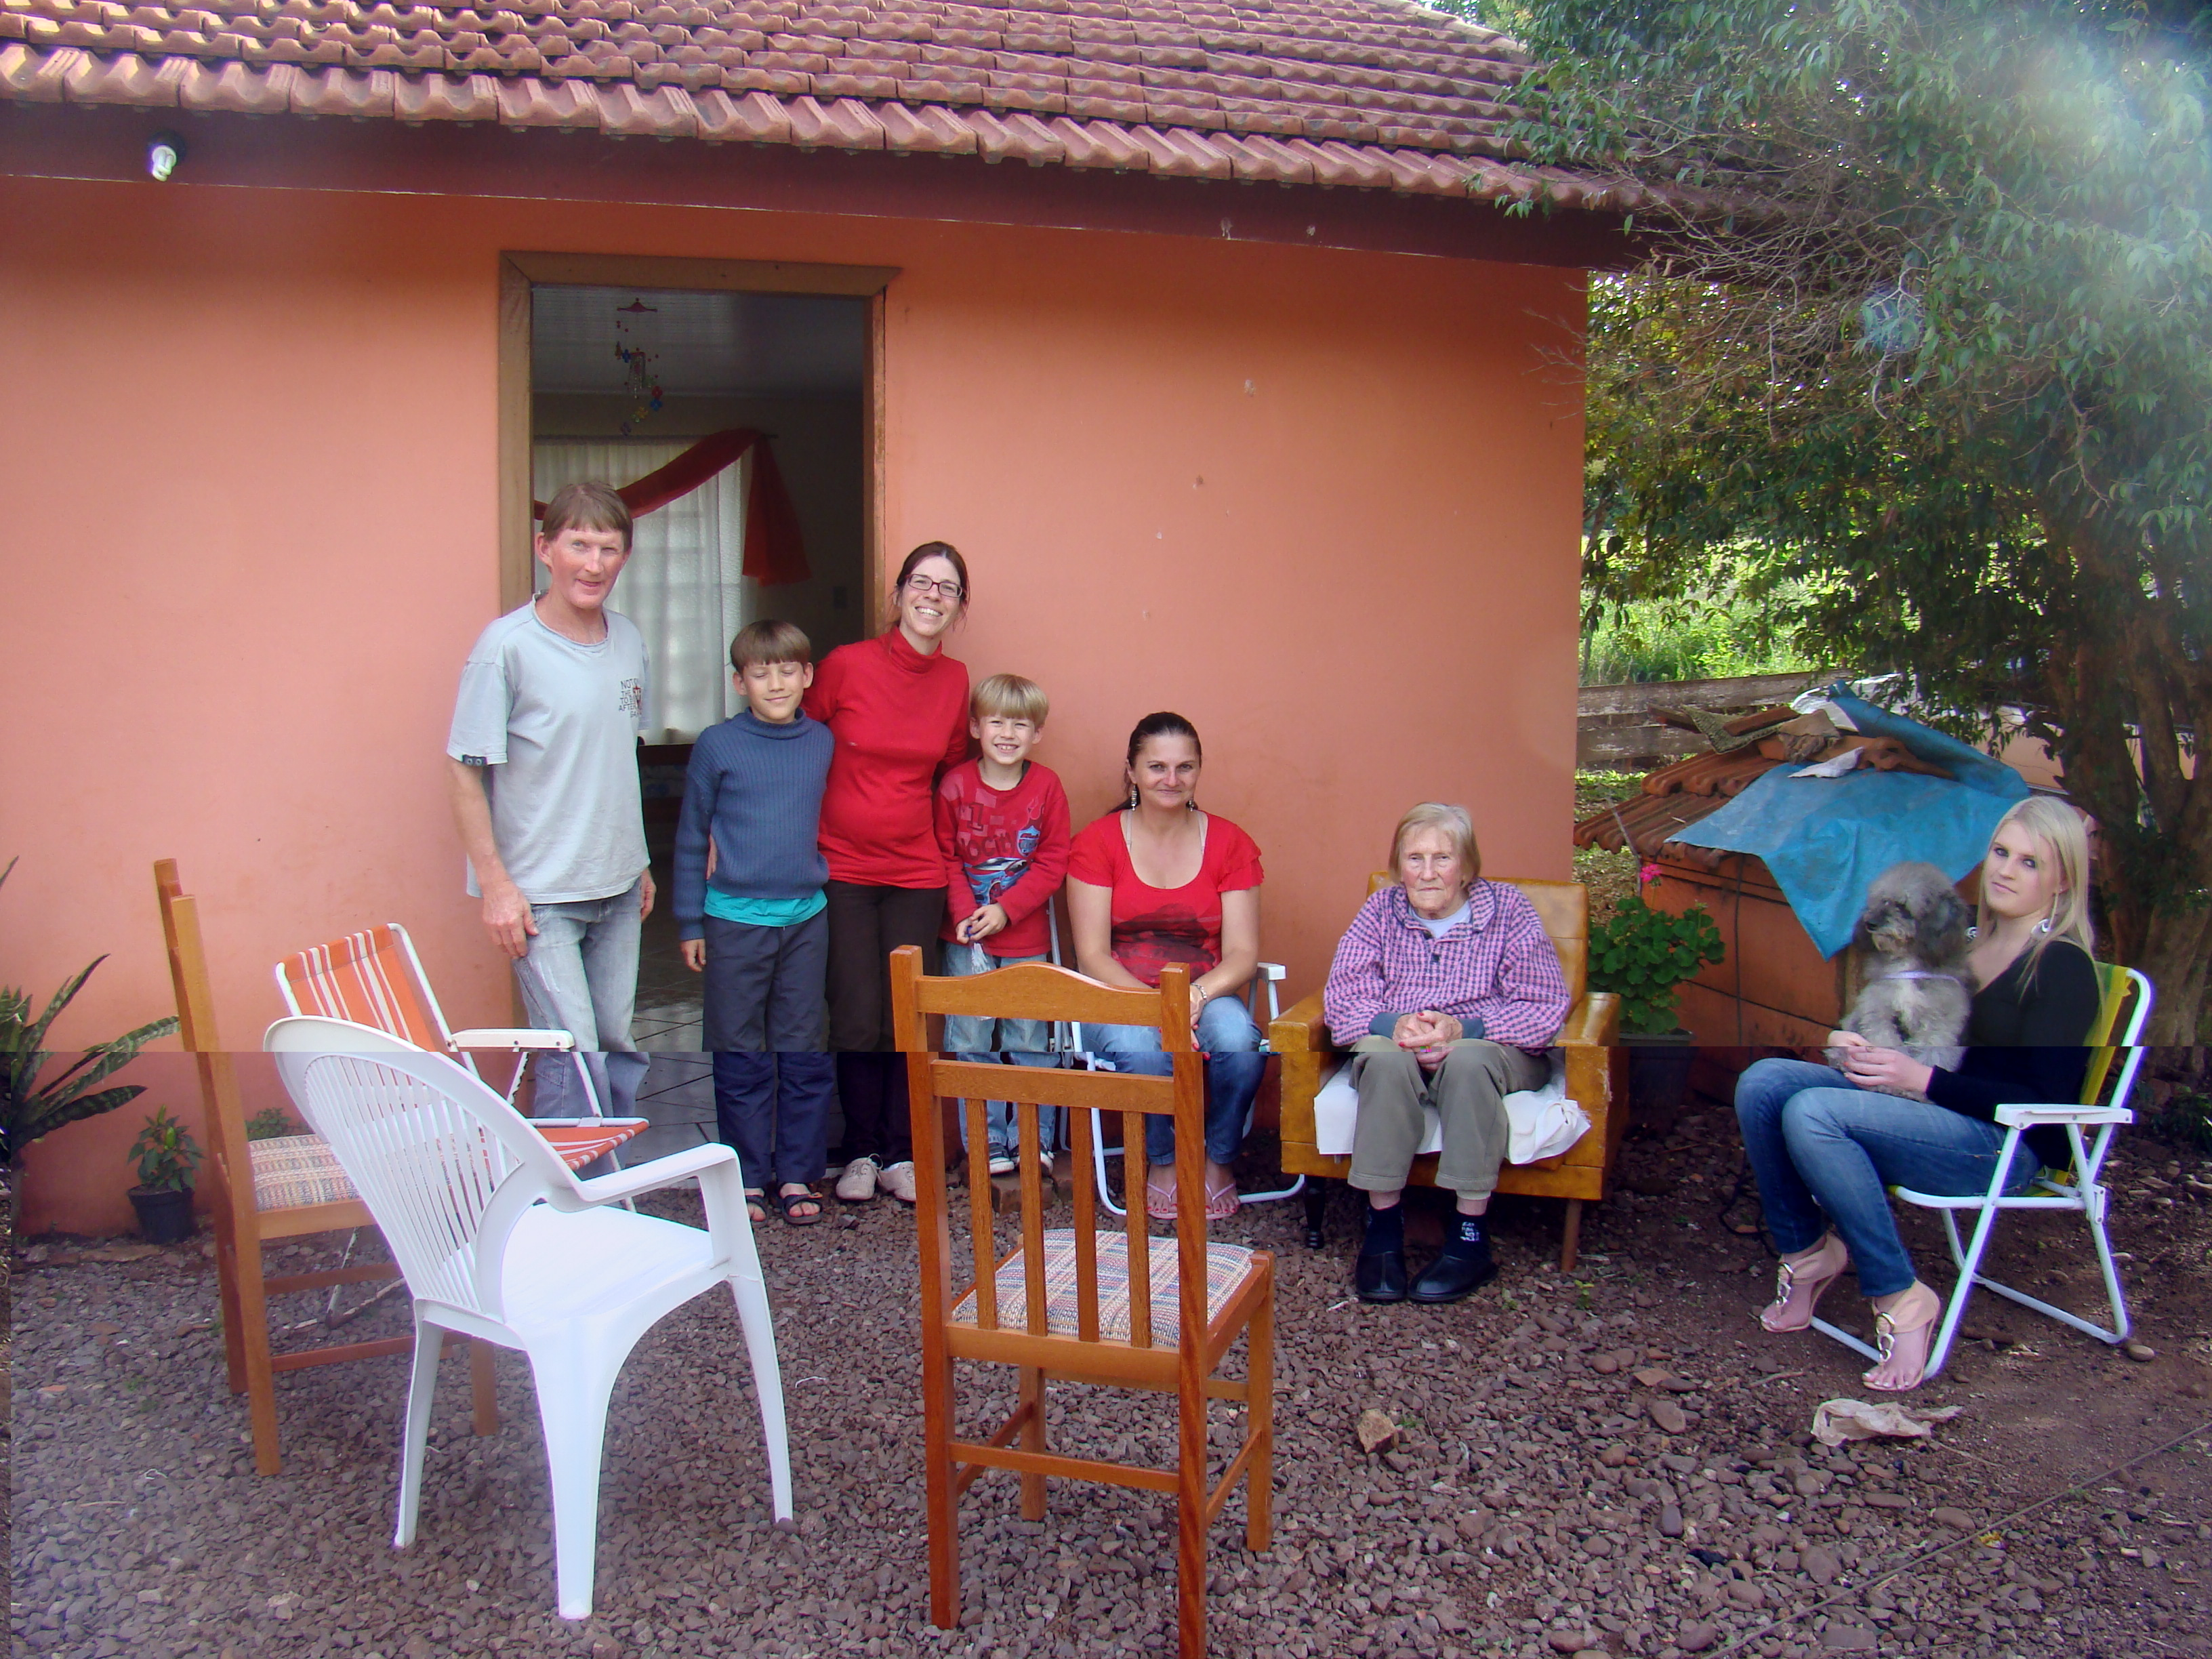
\includegraphics[width=0.85\linewidth,height=\textheight,keepaspectratio,alt={Besuch bei Tante Sunta (Asunda Erna Lohmann, geb. 1921), einer Schwester von Oma Rosita, im September 2012, mit Bárbara, Matheus und Lucas und Familienangehörigen. Im Vordergrund die Stühle des Gesprächs.}]{imagens/lohmann_visita_tia_sunta_2012.jpg}
\caption{Besuch bei Tante Sunta (Asunda Erna Lohmann, geb. 1921), einer
Schwester von Oma Rosita\index[pessoas]{lohmann, rosita erica@Lohmann, Rosita Érica}, im September 2012, mit Bárbara, Matheus und
Lucas und Familienangehörigen. Im Vordergrund die Stühle des Gesprächs.}
\end{figure}

Hier spricht Bárbara.

\emph{Ich wusste nicht genau, was mich erwartete. Es waren die
Geschwister meiner Großmutter, aber ich kannte sie fast nur dem Namen
nach. Was mich ergriff, waren die Gesichter. In jedem von ihnen war
etwas von der Oma: wie sie die Hände faltete, das Kinn, der leicht
misstrauische Blick in die Kamera. Es war, als sähe ich meine Großmutter
auf vier Menschen verteilt. Ich wollte, dass die Jungen genau
hinschauen, auch wenn sie nicht alles verstanden. Ich dachte, eines
Tages würden sie sich daran erinnern wollen, dass sie dort gewesen
sind.}

In jenen Tagen besuchten wir auch die Friedhöfe von Estrela\index[lugares]{estrela@Estrela} und Arroio
do Meio. Ich habe weniger Einzelheiten davon behalten, als mir lieb
wäre, und deshalb stützt sich das, was ich in den folgenden Abschnitten
über die Gräber schreibe, auch auf die Fotografien und die Datenblätter
der CAPEF, des genealogischen Forschungszentrums in Lajeado\index[lugares]{lajeado@Lajeado}, das die
Gründerfamilien von Estrela\index[lugares]{estrela@Estrela} rekonstruiert hat.

\section{\texorpdfstring{Von Harderode auf die
\emph{Hiran}}{Von Harderode\index[lugares]{harderode@Harderode} auf die Hiran}}\label{von-harderode-auf-die-hiran}

\emph{Harderode\index[lugares]{harderode@Harderode}, Herzogtum Braunschweig, September 1846}

Harderode\index[lugares]{harderode@Harderode} ist ein kleines Dorf in den Hügeln östlich der Weser, bei
Hameln\index[lugares]{hameln@Hameln}, der Stadt des Rattenfängers. Dort lebten zu Beginn des 19.
Jahrhunderts Johann Friedrich Christian Lohmann\index[pessoas]{lohmann, johann friedrich christian@Lohmann, Johann Friedrich Christian}, geboren am 23. Oktober
1788, und Sophie Dorothee Elizabeth Schrader\index[pessoas]{schrader, sophie dorothee elizabeth@Schrader, Sophie Dorothee Elizabeth}, geboren am 16. Februar
1796. Sie sind eure fünffachen Urgroßeltern, sieben Generationen über
Matheus und Lucas. Johann Friedrich war Lehrer, laut dem Datenblatt der
CAPEF, und das passt zu dem Stolz, den der Lohmann-Familienverband jener
Gegend auf seine Abstammung hatte. In einem Dokument von 1938 hieß es,
seit einem gewissen Tönnis Lohmann, Schulmeister und Küster um 1640,
habe die Sippe „in allen Verzweigungen'' Lehrer und Pfarrer
hervorgebracht. Ich lese dieses Dokument mit zweifacher Vorsicht. Die
eine ist das natürliche Misstrauen gegenüber jeder Genealogie, die sich
selbst rühmt. Die andere ist das Unbehagen über das Datum: 1938 hatte in
Deutschland das Interesse an Wappen und „Abstammung'' einen
Zusammenhang, den ich nicht übergehen kann. Aber der Beruf des Vaters
von Georg Karl\index[pessoas]{meier, karl@Meier, Karl} Maximilian ist eine einfache Tatsache, und die halte ich
fest.

Ihr Sohn Georg Karl Maximilian Lohmann\index[pessoas]{lohmann, georg karl maximilian@Lohmann, Georg Karl Maximilian} wurde am 12. Juli 1821 in
Harderode\index[lugares]{harderode@Harderode} geboren. Er war Kaufmann. Am 4. September 1846, mit
fünfundzwanzig Jahren, schiffte er sich an Bord der \emph{Hiran} nach
Brasilien ein. Die CAPEF berichtet ein Detail, das ich außergewöhnlich
finde: Die \emph{Hiran} war ein Frachtschiff und hatte außer dem Kapitän
und der Mannschaft nur zwei Passagiere an Bord, Georg Karl\index[pessoas]{meier, karl@Meier, Karl} und einen
Herrn Berwig. Ich vergleiche das mit der \emph{Formosa} von 1913, die
die Haas in der dritten Klasse mit Hunderten anderer Auswanderer
brachte, und mit den Briggs von 1828 und 1847, vollgestopft mit Familien
aus dem Hunsrück\index[lugares]{hunsruck@Hunsrück} und von der Mosel\index[lugares]{mosel@Mosel}. Euer vierfacher Urgroßvater hat den
Atlantik fast allein überquert, zwischen Kisten und Fässern, in einer
Zeit, in der die Reise drei Monate dauerte.

Ich stelle mir die Überfahrt vor, und ich sage dazu, dass es Vorstellung
ist: ein junger Mann aus Braunschweig, Lehrersohn, über die Reling eines
Frachtseglers gebeugt, der sieht, wie das Meer beim Überqueren des
Äquators die Farbe wechselt, und spürt, wie die Luft von Woche zu Woche
feuchter und wärmer wird. Falls er eine Ahnung von Meteorologie hatte,
und ein Lehrersohn hatte sie vielleicht, wird er in der Praxis gelernt
haben, was wir an der Universität lehren: dass der Nordostpassat die
Segelschiffe nach Süden schiebt, dass die äquatoriale Kalmenzone sie
festhält und dass der Südostpassat sie bis an die Küste Brasiliens
trägt. Die \emph{Hiran} erreichte Rio de Janeiro\index[lugares]{rio de janeiro@Rio de Janeiro} am 5. Dezember 1846,
zweiundneunzig Tage nach der Abfahrt.

Das Datenblatt der CAPEF sagt, es sei der Geburtstag der Prinzessin Dona
Isabel gewesen, mit Feierlichkeiten am Hof. Hier muss der Ermittler die
Legende berichtigen. Prinzessin Isabel wurde am 29. Juli 1846 geboren.
Im Dezember hatte sie keinen Geburtstag, sie war ein vier Monate alter
Säugling. Möglicherweise waren die erinnerten Feste die zum Geburtstag
von Kaiser Dom Pedro II. am 2. Dezember, die sich über einige Tage
hinzogen. Möglich ist auch, dass sich das Detail erst später an die
Geschichte geheftet hat. Am Wesentlichen ändert das nichts, aber es
zeigt, wie Familienerzählungen sich mit der Zeit ausschmücken. Auch
dieses Buch wird seine Ausschmückungen haben. Ich hoffe, ihr findet sie.

\begin{ficha}

\textbf{Archivkarte}: Georg Karl Maximilian Lohmann\index[pessoas]{lohmann, georg karl maximilian@Lohmann, Georg Karl Maximilian} (FamilySearch
\texttt{27QQ-TM9}). Geburt: 12.07.1821, Harderode\index[lugares]{harderode@Harderode} (Braunschweig).
Auswanderung: 04.09.1846 auf dem Frachtschiff \emph{Hiran}, mit nur
einem weiteren Passagier (Herr Berwig). Ankunft in Rio de Janeiro\index[lugares]{rio de janeiro@Rio de Janeiro}:
05.12.1846. Heirat: 06.05.1849 in Kaffeeschneis (Picada Café\index[lugares]{picada cafe@Picada Café}, damals São
Leopoldo) mit Bárbara Wingert\index[pessoas]{wingert, barbara@Wingert, Bárbara} (05.07.1828--24.11.1915). Tod: 28.07.1899,
Linha Lenz, Estrela\index[lugares]{estrela@Estrela} (RS). Quelle: CAPEF, \emph{Famílias fundadoras de
Estrela\index[lugares]{estrela@Estrela} --- Família Lohmann}. Vorbehalt: Die Verknüpfung des
Ankunftsdatums mit dem Geburtstag der Prinzessin Isabel ist nicht
haltbar (sie wurde am 29.07.1846 geboren).

\end{ficha}

Von Rio zog Georg Karl\index[pessoas]{meier, karl@Meier, Karl} weiter in den Süden, in die alte Kolonie São
Leopoldo, gegründet 1824. In Kaffeeschneis, der heutigen Gemeinde Picada
Café, heiratete er am 6. Mai 1849 Bárbara Wingert\index[pessoas]{wingert, barbara@Wingert, Bárbara}, geboren am 5. Juli
1828. Ich nenne den Namen eigens, weil er mich beim ersten Lesen lächeln
ließ. Bárbaras dreifache Urgroßmutter hieß ebenfalls Bárbara.

Das Paar hatte zwölf Kinder. Um ihnen Land zu sichern, tätigte Georg
Karl\index[pessoas]{meier, karl@Meier, Karl} 1870 den Kauf, der einem Ort seinen Namen gab. Nach der Geschichte,
die Forscherinnen aus der Region aufgezeichnet haben, verkaufte ihm ein
Grundbesitzer namens Cláudio José Monteiro vierundzwanzig Kolonien Land
in der damaligen Gemeinde Estrela\index[lugares]{estrela@Estrela}, entlang des Flusses Taquari. (Eine
\emph{colônia} war im Süden Brasiliens das übliche Landlos eines
Siedlers.) Die CAPEF spricht von etwa zwölfhundert Hektar, was Kolonien
von je rund fünfzig Hektar ergäbe. Die Größe einer Kolonie schwankte im
Lauf der Zeit, und die Rechnung muss nicht auf den Meter aufgehen. So
entstand die Fazenda Lohmann, heute eine Ortschaft der Gemeinde Roca
Sales, neun Kilometer vom Hauptort entfernt. Es gibt dort eine
evangelische Kirche mit dem Friedhof daneben, einen Tanzsaal, einen 1914
gegründeten Gesangverein und die Tradition der \emph{Kerb}-Bälle, mit
dem alten hausgemachten Ingwerbier, das in den Flaschen knallte. Die
Forscherinnen zählten etwa hundertzwanzig Familien, die meisten
evangelisch.

Zwölf Kinder und vierundzwanzig Kolonien: zwei Kolonien pro Kind. Die
Rechnung ist so rund, dass sie kein Zufall zu sein scheint. Ein
Einwanderer, der aus einem Land kam, in dem die Erbteilung in jeder
Generation die Kinder ohne Boden zurückließ, kaufte auf einen Schlag
genug Land, damit jedes Kind sein eigenes hätte. Im Bayern\index[lugares]{bayern@Bayern} der Haas
bekam der einzige Erbe alles, und die anderen wurden Ziegler und
Arbeiter. Auf der Fazenda Lohmann versuchte ein Vater, dass niemand
fortgehen musste. Es gelang ihm natürlich nicht. Die Enkel verteilten
sich über das Tal, nach Erechim, nach Paraná, und eine Urenkelin landete
in Joinville\index[lugares]{joinville@Joinville}.

Das Fachwerkhaus der Familie wurde abgebaut und im Historischen Park von
Lajeado\index[lugares]{lajeado@Lajeado} wieder aufgebaut, wo es als Museum der Familie Lohmann dient. Es
war Kulisse des Films \emph{A Paixão de Jacobina} über den Aufstand der
Mucker, die religiösen Konflikte, die 1874 die Kolonie São Leopoldo\index[lugares]{sao leopoldo@São Leopoldo}
erschütterten. Ich mag diese Ironie: das Haus einer braven lutherischen
Familie, gefilmt als Schauplatz eines Schismas. Georg Karl\index[pessoas]{meier, karl@Meier, Karl} starb am 28.
Juli 1899 in der Linha Lenz, Bárbara Wingert\index[pessoas]{wingert, barbara@Wingert, Bárbara} am 24. November 1915. Ihre
Gräber liegen auf dem kleinen Friedhof der Linha Winck in Estrela\index[lugares]{estrela@Estrela}, Seite
an Seite: zuerst ihres, dann seines, auf den Fotografien der CAPEF.
Georg Karls Bruder Georg August Christian, der 1848 mit seiner Schwester
Karoline kam, liegt auf dem Friedhof von Novo Paraíso, ebenfalls in
Estrela\index[lugares]{estrela@Estrela}, neben seiner Frau Katharina Ballus.

\section{Sechsundzwanzig Tage}\label{sechsundzwanzig-tage}

\emph{Arroio do Meio\index[lugares]{arroio do meio@Arroio do Meio}, Dezember 1889}

Das dritte Kind von Georg Karl\index[pessoas]{meier, karl@Meier, Karl} und Bárbara war Friedrich Lohmann\index[pessoas]{lohmann, friedrich@Lohmann, Friedrich},
geboren am 18. Februar 1853 in Estrela\index[lugares]{estrela@Estrela}. Er ist euer dreifacher
Urgroßvater. Er heiratete ein Mädchen aus einer anderen
Einwandererfamilie, Suzana Regina Schnack\index[pessoas]{schnack, suzana regina@Schnack, Suzana Regina}, geboren am 9. Juli 1858.

Die Schnacks kamen aus dem äußersten Norden Deutschlands, aus
Schleswig-Holstein, dem Land zwischen den Meeren. Julius Georg Schnack\index[pessoas]{schnack, julius georg@Schnack, Julius Georg}
wurde dort am 16. Februar 1830 geboren, als Sohn von Peter Friedrich
Ludwig Schnack und Regine Marie Wacker\index[pessoas]{wacker, regine marie@Wacker, Regine Marie}. Am 8. März 1857 heiratete er
Susanna Charlotte Köhnlein\index[pessoas]{kohnlein, susanna charlotte@Köhnlein, Susanna Charlotte} und hatte sieben Kinder in Estrela\index[lugares]{estrela@Estrela} und Arroio
do Meio. Zwei der Töchter heirateten zwei Lohmann-Brüder: Suzana Regina
den Friedrich, Elisa Sophie den August Georg. In den Kolonien war das
üblich. Familien, die zusammen ankamen, sich beim Roden halfen und sich
im Gottesdienst trafen, waren am Ende durch mehr als einen Faden
verbunden. Julius Georg wurde vierundneunzig Jahre alt und starb 1924 in
Arroio do Meio\index[lugares]{arroio do meio@Arroio do Meio}. Susanna Charlotte starb 1926 mit einundneunzig.

Ihre Tochter hatte nicht dasselbe Glück. Friedrich und Suzana Regina
hatten fünf Kinder: Júlio Carlos (1881), Alberto Jorge (1886), Berta
Guilhermina (1888), Adolfo André und Francisco Jacob, beide als 1889
geboren angegeben. Francisco Jacob kam am 20. November 1889 zur Welt.
Ich weiß nicht, ob Adolfo André sein Zwilling war oder Anfang jenes
Jahres geboren wurde und das Datum falsch ist. Das ist eine Frage an die
Taufbücher. Am 16. Dezember 1889, sechsundzwanzig Tage nach der Geburt,
starb Suzana Regina in Arroio do Meio\index[lugares]{arroio do meio@Arroio do Meio}. Sie war einunddreißig.

Der Eintrag sagt nicht, woran. In den 1880er-Jahren, in einer Kolonie im
Landesinneren von Rio Grande do Sul, war die wahrscheinlichste Ursache
eines solchen Todes, Wochen nach einer Geburt, das Kindbettfieber, eine
Infektion, die die Medizin der Zeit kaum verstand und die überall junge
Frauen tötete. Aber es ist eine Vermutung. Die Tatsache ist diese:
Friedrich wurde mit sechsunddreißig Jahren Witwer, mit fünf Kindern, das
jüngste keinen Monat alt. Soweit ich weiß, heiratete er nicht wieder,
und er lebte bis 1937. Wer zog Francisco Jacob auf? Eine ältere
Schwester, eine Schnack-Tante, eine Nachbarin mit Milch? Ich weiß es
nicht. Dieser ohne Mutter aufgewachsene Junge ist der junge Mann mit dem
Schnurrbart auf dem Hochzeitsbild von 1914.

In diesem Buch gibt es eine Entsprechung, die ich nicht geplant habe und
die mich beeindruckt hat, als ich sie bemerkte. In Kapitel 10 stirbt
Anna Eller\index[pessoas]{eller, anna@Eller, Anna} kurz nach der Geburt von Fernando Dörner\index[pessoas]{dorner, fernando@Dörner, Fernando}, dem Jüngsten, um
1898. Hier, neun Jahre früher, stirbt Suzana Regina Schnack\index[pessoas]{schnack, suzana regina@Schnack, Suzana Regina}
sechsundzwanzig Tage nach der Geburt von Francisco Jacob, dem Jüngsten.
Die beiden mutterlosen Jungen wuchsen Hunderte Kilometer voneinander
entfernt auf, ohne sich je zu kennen. Der eine wurde Bárbaras
Urgroßvater, der andere mein Großvater. In euch beiden, Matheus und
Lucas, treffen sich diese zwei Verluste.

\begin{ficha}

\textbf{Archivkarte}: \emph{Recenseamento do Brasil realizado em 1º de
setembro de 1920} (Volkszählung Brasiliens vom 1. September 1920), Bd.
III (Landwirtschaft), Verzeichnis der Eigentümer landwirtschaftlicher
Betriebe in Rio Grande do Sul (Rio de Janeiro\index[lugares]{rio de janeiro@Rio de Janeiro}, 1924). Unter den
Vorkommen des Familiennamens: „Adolpho André Lohmann'' (wahrscheinlich
der Bruder von Francisco Jacob), eine „Linha Lohmann'', „Frederico
Lohmann'' und „Frederico H. Lohmann'' (einer von ihnen vielleicht
Friedrich, damals 67 Jahre alt; die Gemeinde ließ sich nicht
bestätigen), außerdem Eigentümer namens Schnack und Endres. Die Liste
nennt keine Verwandtschaftsverhältnisse; die Zuordnungen sind
Hypothesen.

\end{ficha}

\section{Die Zwölf von Palmas}\label{die-zwuxf6lf-von-palmas}

\emph{Palmas\index[lugares]{palmas@Palmas}, Arroio do Meio\index[lugares]{arroio do meio@Arroio do Meio}, Mitte der 1930er-Jahre}

Francisco Jacob Lohmann\index[pessoas]{lohmann, francisco jacob@Lohmann, Francisco Jacob} heiratete Miguelina Leocádia Endres\index[pessoas]{endres, miguelina leocadia@Endres, Miguelina Leocádia} am 5.
September 1914. Sie war am 9. Dezember 1891 geboren, in einer
Endres-Familie aus dem Tal, deren Geschichte ich noch nicht gründlich
erforscht habe. Die Volkszählung von 1920 verzeichnet mindestens zwei
Eigentümer namens Endres in Rio Grande do Sul, aber ich weiß nicht,
welcher von ihnen, wenn überhaupt einer, ihr Vater war. Das Paar hatte
zwölf Kinder, und die Liste, die ich vom vielen Nachprüfen auswendig
kann, verdient es, vollständig aufgeschrieben zu werden, denn es ist die
Liste von Bárbaras Großonkeln und Großtanten: Walter Érico, Reinholdo,
Urbano Aldo, Armando Ernesto, Walter Erich, Blanca Erna, Albano Paulo,
Rosita Érica, Eldo Astor, Asunda Erna, Dulsa Iria und Arlindo Erno.

Ich schulde euch allerdings ein Geständnis des Ermittlers. Die Daten,
die die Register diesen zwölf Namen zuordnen, gehen nicht auf. Walter
Érico erscheint als 1911 geboren und Reinholdo als 1912, also vor der
Hochzeit von 1914. Es gibt zwei Walter, einen von 1911 und einen vom 27.
Dezember 1916, im selben Jahr wie Armando. Drei Kinder erscheinen als
1918 geboren, darunter Rosita, und zwei als 1921. Manche Daten sind wohl
nur ungefähr, eingetragen von jemandem, der sie aus dem Gedächtnis
errechnet hat. Und ich kann nicht ausschließen, dass die beiden Walter
eine einzige Person sind, die zweimal erfasst wurde, ein häufiger Fehler
in gemeinschaftlich gepflegten Stammbäumen. Die Familie sagt zwölf, und
ich schreibe zwölf, aber die Warnung lasse ich hier stehen.

Die kostbarste Fotografie dieses Zweigs hat mir geholfen, über das
Problem nachzudenken. Es ist ein Gruppenbild, sehr viel später
koloriert, mit einem darunter geklebten Zettel: „Família de Francisco
Jacob Lohmann casado com Miguelina Leocádia Endres\index[pessoas]{endres, miguelina leocadia@Endres, Miguelina Leocádia} Lohmann. (Foto por
ocasião da conclusão da casa nova em Palmas\index[lugares]{palmas@Palmas} -- Arroio do Meio\index[lugares]{arroio do meio@Arroio do Meio})``, also:
Familie von Francisco Jacob Lohmann\index[pessoas]{lohmann, francisco jacob@Lohmann, Francisco Jacob}, verheiratet mit Miguelina Leocádia
Endres Lohmann, Foto anlässlich der Fertigstellung des neuen Hauses in
Palmas\index[lugares]{palmas@Palmas}, Arroio do Meio\index[lugares]{arroio do meio@Arroio do Meio}. Die Eltern sitzen in der Mitte, sie in einem
dunklen Kleid mit weißem Spitzenkragen, er in einem blauen Anzug und mit
Schnurrbart, inzwischen ergraut, derselbe junge Mann vom Bild von 1914,
zwanzig und etliche Jahre später. Um sie herum die Kinder: die jungen
Frauen in Kleidern, die jungen Männer in Anzug und Krawatte, zwei
Mädchen mit Topfschnitt und Matrosenbluse, zwei Jungen in Knopfhemden.
Ich habe gezählt und nachgezählt: Es sind dreizehn Personen, die Eltern
und elf Kinder. Die Bildunterschrift nennt die elf Namen, und darunter
ist nur ein Walter, Walter Érico. Sie schreibt außerdem „Urbano Arno'',
wo die Register „Urbano Aldo'' haben, und „Reinboldo'', wo sie
„Reinholdo'' haben. Nach dem Alter der Kleinsten scheint der Jüngste,
Arlindo, geboren 1924, etwa zehn oder zwölf Jahre alt zu sein, und
deshalb setze ich das Foto in die Mitte der 1930er-Jahre. Rosita steht
ganz rechts, eine junge Frau mit breitem, ernstem Gesicht in einem
bestickten blauen Kleid.

\begin{figure}
\centering
\includegraphics[width=0.85\linewidth,height=\textheight,keepaspectratio,alt={Die Familie von Francisco Jacob Lohmann und Miguelina Leocádia Endres Lohmann vor dem neuen Haus in Palmas, Arroio do Meio (RS), wahrscheinlich Mitte der 1930er-Jahre. Laut der ursprünglichen Bildunterschrift von links nach rechts: Blanca Erna, Armando Ernesto, Urbano, Reinholdo, Walter Érico, Arlindo Erno, Eldo Astor, Asunda Erna, Miguelina, Dulsa Iria, Francisco Jacob, Albano Paulo und Rosita Érica, die spätere Oma Rosita, ganz rechts.}]{imagens/lohmann_familia_completa_palmas_arroio_do_meio.jpg}
\caption{Die Familie von Francisco Jacob Lohmann und Miguelina Leocádia
Endres Lohmann vor dem neuen Haus in Palmas\index[lugares]{palmas@Palmas}, Arroio do Meio\index[lugares]{arroio do meio@Arroio do Meio} (RS),
wahrscheinlich Mitte der 1930er-Jahre. Laut der ursprünglichen
Bildunterschrift von links nach rechts: Blanca Erna, Armando Ernesto,
Urbano, Reinholdo, Walter Érico, Arlindo Erno, Eldo Astor, Asunda Erna,
Miguelina, Dulsa Iria, Francisco Jacob, Albano Paulo und Rosita Érica,
die spätere Oma Rosita\index[pessoas]{lohmann, rosita erica@Lohmann, Rosita Érica}, ganz rechts.}
\end{figure}

Die andere Fotografie zeigt das Haus selbst. Es ist ein weißes
zweistöckiges Haus mit hohem, steilem Dach und einer Dachgaube, einer
Veranda mit Säulen und weißem Geländer voller Blumentöpfe und einem
hohen gemauerten Sockelgeschoss, das sich zum Gefälle des Geländes
öffnet. Die Familie steht aufgereiht entlang der Fassade, klein vor dem
Bau. Die Erde ringsum ist noch kahl, von der Baustelle aufgewühlt.
Dahinter ein bewaldeter Hügel und das offene Tal. Ich stelle mir den
Stolz jenes Tages vor, und hier ist das Wort „vorstellen'' ehrlich: ein
Mann, der ohne Mutter geboren wurde, in einer Kolonie, in der sein
Großvater vierundzwanzig Kolonien für seine Kinder gekauft hatte,
versammelt die elf oder zwölf Kinder, die er hatte, vor dem Haus, das er
für sie gebaut hatte.

\begin{figure}
\centering
\includegraphics[width=0.85\linewidth,height=\textheight,keepaspectratio,alt={Das neue Haus der Familie Lohmann in Palmas, Arroio do Meio, frisch fertiggestellt, mit der Familie vor der Veranda. Das Haus liegt auf 45 Metern Höhe, gegenüber dem Salto, der Stromschnelle des Taquari.}]{imagens/lohmann_casa_nova_palmas_arroio_do_meio.jpg}
\caption{Das neue Haus der Familie Lohmann in Palmas, Arroio do Meio,
frisch fertiggestellt, mit der Familie vor der Veranda. Das Haus liegt
auf 45 Metern Höhe, gegenüber dem Salto, der Stromschnelle des Taquari.}
\end{figure}

Zu diesem Bild lasse ich Bárbara sprechen.

\emph{Was mich beeindruckt, ist, dass alle für das Foto eines Hauses so
herausgeputzt sind. Die Jungen in zugeknöpften Hemden, die Mädchen mit
Matrosenschleife, der Urgroßvater im Anzug. Als wäre das Haus ein
Familienmitglied, das gerade angekommen ist. Und ich glaube, das war es.
Oma Rosita\index[pessoas]{lohmann, rosita erica@Lohmann, Rosita Érica} ist von dort weggegangen, hat einen Lehrer geheiratet, in
Estrela\index[lugares]{estrela@Estrela} und in Nova Petrópolis\index[lugares]{nova petropolis@Nova Petrópolis} gelebt und ist am Ende in Joinville\index[lugares]{joinville@Joinville}
gelandet. Aber in diesem weißen Haus war sie ein junges Mädchen.}

Die Kinder von Francisco und Miguelina gingen den Weg aller großen
Familien der Kolonie. Einige blieben im Tal, andere zogen fort. Rosita
heiratete Erno Hoeveler\index[pessoas]{hoeveler, erno@Hoeveler, Erno} und lebte an den Schulen, an denen er
unterrichtete. Arlindo heiratete 1949 Hilda Rahmeier, lebte in Estrela\index[lugares]{estrela@Estrela}
und starb dort. Die anderen kenne ich nur aus den Namen und den Fotos
von 2012. Ein Kommentar, den ein Nachkomme in einem Blog zur Geschichte
des Tals hinterlassen hat, bewahrt eine Episode dieser Zerstreuung, die
ich nicht kannte. Júlio Carlos Lohmann, der älteste Bruder von Francisco
Jacob, soll in Erechim einen Hof besessen haben, der während der
Revolution von 1923 überfallen wurde, dem Bürgerkrieg in Rio Grande do
Sul zwischen den Chimangos, den Anhängern der Landesregierung, und den
aufständischen Maragatos. Er, seine Frau und die drei Kinder sollen mit
Schüssen vertrieben worden sein und auf der Fazenda Lohmann, beim
Großvater und den Onkeln, in Roca Sales Zuflucht gefunden haben, bevor
sie sich in Estrela\index[lugares]{estrela@Estrela} niederließen. Ich halte es fest, wie ich es bekommen
habe: ein Familienzeugnis, ohne Dokument, das es bestätigt. Aber es
zeigt, welche Aufgabe das 1870 gekaufte Land fünfzig Jahre später noch
hatte: Es war der Ort, an den man zurückkehrte, wenn alles schiefging.

\section{Der Fluss vor dem Haus}\label{der-fluss-vor-dem-haus}

Der Salto do Taquari in Palmas\index[lugares]{palmas@Palmas} liegt genau gegenüber dem Haus. Für
jemanden, der baut, ist ein solcher Fluss ein großzügiger Nachbar. Er
bringt die fruchtbare Erde der Auen, treibt Mühlen an und war lange die
Straße, auf der die Dampfer die Ernten des Tals nach Porto Alegre
brachten. Die Kolonisten am Taquari ließen sich, wie die am Itajaí\index[lugares]{itajai@Itajaí} und
am Tubarão\index[lugares]{tubarao@Tubarão}, aus guten Gründen am Wasser nieder.

Aber die Flüsse des Südens haben lange Launen. Der Taquari entspringt
unter dem Namen Rio das Antas auf den Hochflächen der Serra und sammelt
den Regen eines riesigen Einzugsgebiets mit steilen Hängen. Wenn eine
Kaltfront langsam über Rio Grande do Sul hinwegkriecht, gespeist von der
Feuchtigkeit, die der Low-Level-Jet aus Amazonien östlich der Anden
heranführt, oder wenn sich über dem Bundesstaat ein außertropischer
Zyklon bildet und an einem Tag den Regen eines Monats ausschüttet, dann
strömt all dieses Wasser in wenigen Stunden im Tal zusammen. Der Fluss
steigt um Meter. Diese Meteorologie kenne ich gut, denn ich habe einen
großen Teil meines Berufslebens damit verbracht, sie vorherzusagen und
zu modellieren, am Itajaí\index[lugares]{itajai@Itajaí} und am Taquari.

Im Mai 1941, wenige Jahre nach dem Foto vom neuen Haus, hatte der
Taquari eines der größten Hochwasser seiner aufgezeichneten Geschichte.
Das gesamte Einzugsgebiet des Guaíba trat über die Ufer, und Porto
Alegre stand wochenlang unter Wasser. Die zwölf Geschwister von Palmas\index[lugares]{palmas@Palmas}
waren damals zwischen siebzehn und dreißig Jahre alt. Sehr
wahrscheinlich haben alle dieses durch das Tal steigende Wasser im
Gedächtnis behalten, und das Hochwasser von 41 wurde, wie für alle
Familien am Taquari, zum Maß aller anderen. Ich habe jedoch keinen
Bericht von ihnen darüber. Ich habe 2012 nicht gefragt. Heute würde ich
zuerst danach fragen.

Das topografische Profil, das ich Jahre später erstellt habe, setzt die
Casa Lohmann auf fünfundvierzig Meter Höhe, gegenüber dem Salto. In
dieses Profil habe ich die Linien der großen Hochwasser eingezeichnet,
das von 1941 und die späteren. Was die Zeichnung zeigt, erzähle ich hier
nicht. Diese Geschichte gehört ins nächste Kapitel, zusammen mit der des
Tubarão\index[lugares]{tubarao@Tubarão} und der des Itajaí\index[lugares]{itajai@Itajaí}, denn die drei sind dieselbe Geschichte. Ich
sage nur, was in Brasilien jeder aus den Zeitungen erfuhr. Im September
2023 schüttete ein außertropischer Zyklon über dem Taquari-Tal einen
Regen aus, der Dutzende Menschen tötete, und Roca Sales, wo die Fazenda
Lohmann liegt, Muçum und Arroio do Meio\index[lugares]{arroio do meio@Arroio do Meio}, wo Palmas\index[lugares]{palmas@Palmas} liegt, wurden
verwüstet. Im November 2023 stieg der Fluss erneut. Im Mai 2024, bei der
größten Klimakatastrophe in der Geschichte von Rio Grande do Sul, stieg
er noch einmal, höher, als sich irgendjemand erinnerte.

Onkel Arlindo lebte nicht mehr, um es zu sehen. Er starb im Februar
2018, in demselben Monat, in dem ich die Bücher von Maxhütte-Haidhof\index[lugares]{maxhutte-haidhof@Maxhütte-Haidhof}
aufschlug. Von den anderen Geschwistern kenne ich die Daten nicht, und
ich werde keine vermuten. Aber als ich 2023 und 2024 im Fernsehen die
Bilder von Roca Sales und Arroio do Meio\index[lugares]{arroio do meio@Arroio do Meio} unter dem Schlamm sah, suchte
ich als Erstes auf der Karte zwei Koordinaten: die der Fazenda Lohmann
und die des weißen Hauses gegenüber dem Salto. Dann suchte ich die Fotos
vom September 2012 heraus, die Veranden, die Stühle im Kreis, die
Kieshöfe. Es waren dieselben Orte.

Hier beschließt Bárbara den Teil IV.

\emph{Ich sehe mir das Profil des Hauses an, mit den Hochwasserlinien
darüber, und es fällt mir schwer, die beiden Bilder zusammenzubringen.
Das Haus ist das vom Foto, auf dem alle ihre Sonntagskleider tragen. Ich
dachte an meine Großonkel und Großtanten, an die Stühle um Tante Sunta,
und ich dachte, dass wir rechtzeitig gekommen waren, um die Menschen zu
sehen, aber nicht wussten, dass wir auch rechtzeitig kamen, um die Orte
noch so zu sehen, wie sie waren.}

Ihr beide, Matheus und Lucas, wart an diesen Orten, als ihr klein wart.
Ihr seid auf den Fotos, im roten T-Shirt und im blauen Pullover, auf dem
Arm eines Vaters und auf einem Stuhl stehend, neben Onkeln und Tanten,
die vor dem Ersten Weltkrieg geboren waren. Vielleicht erinnert ihr euch
nicht. Deshalb habe ich dieses Kapitel geschrieben. Das nächste beginnt,
wo dieses endet: beim steigenden Wasser und bei den Familien, die seit
fast zwei Jahrhunderten ihre Häuser an seinem Ufer bauen.

\section{Für euch zum Entdecken}\label{fuxfcr-euch-zum-entdecken-11}

\begin{itemize}
\tightlist
\item
  War Adolfo André der Zwilling von Francisco Jacob, oder wurde er
  Anfang 1889 geboren und das Datum ist falsch? Die Taufbücher können es
  sagen.
\item
  Wer zog Francisco Jacob nach dem Tod von Suzana Regina am 16. Dezember
  1889 auf?
\item
  Gab es unter den Kindern von Francisco und Miguelina zwei Walter oder
  nur einen, der zweimal erfasst wurde? Die Bildunterschrift des Fotos
  aus Palmas\index[lugares]{palmas@Palmas} nennt nur Walter Érico.
\item
  Was haben die Geschwister von Palmas\index[lugares]{palmas@Palmas} vom Hochwasser im Mai 1941 im
  Gedächtnis behalten? Ich habe 2012 nicht gefragt. Fragt die Nachkommen
  von Onkel Urbano, Onkel Armando, Tante Sunta und Onkel Arlindo.
\end{itemize}

\part{Drei Flüsse, das Klima und ein
Erbe}\label{drei-fluxfcsse-das-klima-und-ein-erbe}

\begin{boletim}

Hochwasserwarnung für die Einzugsgebiete von Tubarão\index[lugares]{tubarao@Tubarão}, Itajaí\index[lugares]{itajai@Itajaí} und
Taquari; Hagel auf der Insel. Wiederkehrperiode: eine Generation.

\end{boletim}

\chapter{Drei Flüsse, ein einziger Regen}\label{cap-13}

\emph{28,5° S · 49,0° W, Tubarão\index[lugares]{tubarao@Tubarão}, SC · 27,4° S · 49,6° W, Ituporanga\index[lugares]{ituporanga@Ituporanga}, SC
· 29,3° S · 51,9° W, Palmas\index[lugares]{palmas@Palmas}, Arroio do Meio\index[lugares]{arroio do meio@Arroio do Meio}, RS}

\begin{quote}
\emph{Ein Fluss vergisst seinen Weg nicht; vergessen tun wir.}
\end{quote}

Das schlimmste Hochwasser, das Santa Catarina bis dahin erlebt hatte,
kam 1974, in einem La-Niña-Jahr, als der Süden theoretisch hätte
trockener sein müssen.

\section{Die Karte auf dem Tisch}\label{die-karte-auf-dem-tisch}

Seit ich mit dieser Spurensuche begonnen habe, geht mir eine Karte nicht
aus dem Kopf, und sie hat weder Gemeindegrenzen noch Pfarreinamen. Es
ist eine Karte der Flusseinzugsgebiete. Wenn ich sie auf dem Küchentisch
ausbreite, wie ich es so oft mit den Wetterkarten gemacht habe, die die
Jungen überall im Haus herumliegen sahen, erscheinen drei blaue Linien,
die vom Gebirge zum Meer hinabführen, und neben jeder eine Handvoll
Familiennamen.

Die erste ist der Rio Tubarão\index[lugares]{tubarao@Tubarão}, der von der Serra Geral herabkommt und
sich in die Lagunen von Laguna\index[lugares]{laguna@Laguna} ergießt. Über Laguna, so sagt die
Familienüberlieferung, kamen Johann und Maria 1913 nach Santa Catarina;
die Dokumente belegen vorerst nur, dass sie in Rio de Janeiro\index[lugares]{rio de janeiro@Rio de Janeiro} an Land
gingen. Die zweite ist der Itajaí\index[lugares]{itajai@Itajaí} mit seinen drei Armen, die sich im
Alto Vale, dem oberen Itajaí\index[lugares]{itajai@Itajaí}-Tal, vereinigen, wo \emph{Fata\index[pessoas]{haas, johann@Haas, Johann}} und
\emph{Mota\index[pessoas]{meier, maria@Meier, Maria}} in Rio Novo\index[lugares]{rio novo@Rio Novo} Wald rodeten, die Hauptkirche von Ituporanga\index[lugares]{ituporanga@Ituporanga}
errichteten und in Aurora\index[lugares]{aurora@Aurora} alt wurden, und wo mein Vater Baldoíno sich in
Vidal Ramos\index[lugares]{vidal ramos@Vidal Ramos} niederließ. Ein Stück daneben fließt der Itajaí\index[lugares]{itajai@Itajaí}-Mirim, der
an Brusque\index[lugares]{brusque@Brusque} vorbeizieht, wo Fernando Dörner\index[pessoas]{dorner, fernando@Dörner, Fernando} und Gertrudes Preiss\index[pessoas]{preiss, gertrudes@Preiss, Gertrudes} ruhen,
die Eltern meiner Mutter. Die dritte blaue Linie ist der Taquari in Rio
Grande do Sul, der als Rio das Antas auf den Hochflächen der Serra
entspringt und zwischen Felswänden eingezwängt hinabläuft, bis er sich
auf der Höhe von Roca Sales, Arroio do Meio\index[lugares]{arroio do meio@Arroio do Meio}, Lajeado\index[lugares]{lajeado@Lajeado} und Estrela\index[lugares]{estrela@Estrela} zur Aue
weitet. Dort liegen die Fazenda Lohmann, das Haus in Palmas\index[lugares]{palmas@Palmas}, die Gräber
der Linha Lenz und fast alles, was Bárbara von der Seite ihrer
Großmutter geerbt hat.

Jahrelang habe ich diese drei Linien als Genealoge betrachtet. Erst
später, ein wenig beschämt über die Verspätung, merkte ich, dass ich sie
auch als Meteorologe ansah. Die drei Flüsse, die die Geschichte meiner
Söhne durchziehen, gehören zu den am besten untersuchten Flüssen
Südbrasiliens, gerade weil sie zu denen gehören, die am häufigsten über
die Ufer treten. Jeder hat sein Gespensterhochwasser, das die Alten nur
mit der Jahreszahl nennen, ohne mehr sagen zu müssen: „das von 74'',
„das von 83'', „das von 41''. In den letzten Jahren hat jeder ein neues
Datum bekommen, das er neben das alte stellen kann.

Meine Arbeit an der Universität kreist seit Langem darum, diese
Wassermassen vorherzusagen: Modelle, die sagen, wie viel Regen fallen
wird, die Regen in Abfluss umrechnen und den Abfluss über das Gelände
verteilen. Dies ist kein Fachbericht, aber ich kann nicht über diese
drei Täler schreiben und so tun, als wüsste ich nicht, was ich weiß. Das
wäre, als beschriebe ich das Hochzeitsbild von Francisco und Miguelina,
ohne zu sagen, dass es an einer Wand hängt, die das Wasser schon
erreicht hat.

Der Titel dieses Kapitels ist eine Provokation des Lehrers. Es gab nicht
einen einzigen Regen über Tubarão\index[lugares]{tubarao@Tubarão} 1974, dem Itajaí\index[lugares]{itajai@Itajaí} 1983 und dem Taquari
2024. Aber es gibt eine einzige Maschine, die diese Regenfälle erzeugt,
und bevor ich jeden Fluss besuche, muss ich ihren Deckel öffnen.

\section{Die Regenmaschine}\label{die-regenmaschine}

Stellt euch, wie ich es von meinen Studierenden verlange, einen Fluss
vor, den man nicht sieht. Östlich der Anden, zwischen Bolivien, Paraguay
und dem Norden Argentiniens, weht zu bestimmten Zeiten ein schmales Band
starken Windes in etwas mehr als einem Kilometer Höhe. Die Meteorologen
nennen es Low-Level-Jet, einen Strahlstrom der unteren Atmosphäre. Er
entsteht aus der warmen, feuchten Luft Amazoniens, die die Passatwinde
nach Westen schieben, bis sie gegen die Andenmauer prallt; da sie nicht
hinüberkommt, biegt die Luft nach Süden ab und fließt an der Kordillere
entlang wie Wasser in einer Rinne. Es ist ein Fluss in der Luft, und er
trägt als Wasserdampf mehr Wasser als viele echte Flüsse in ihrem Bett.
Wenn dieser Jet den Süden des Kontinents erreicht und auf einen
Mechanismus trifft, der die Luft zum Aufsteigen zwingt, kondensiert der
Dampf, und Amazonien fällt als Regen über Paraguay, Rio Grande do Sul
und Santa Catarina.

Der häufigste Hebungsmechanismus hier ist die Kaltfront. Eine polare
Luftmasse rückt von Süden vor, dichter als die tropische Luft, schiebt
sich wie ein Keil unter sie und hebt sie an. Meistens zieht die Front
durch: Es regnet einen Tag, der Wind dreht auf Süd, der Himmel klart
auf, und die Temperatur fällt. Die Gefahr liegt bei den Fronten, die
stehen bleiben. Wenn die kalte Luft nicht die Kraft hat weiterzuziehen
und die warme nicht die Kraft, sie zurückzudrängen, verharrt die Front
tagelang über demselben Landstreifen, von hinten gespeist vom
Low-Level-Jet wie von einem Gartenschlauch, den jemand offen gelassen
hat. Man nennt das eine quasistationäre Front, und sie hat die üble
Angewohnheit, sich genau entlang der Einzugsgebiete des Südens
auszurichten.

Die dritte Figur ist der außertropische Zyklon. Entlang der Fronten, vor
allem nahe der Küste von Uruguay und Rio Grande do Sul, fällt der
Luftdruck manchmal stark ab, und die Luft beginnt im Uhrzeigersinn zu
kreisen, dem Drehsinn der Zyklone auf der Südhalbkugel. Ein solcher
Zyklon bündelt die ganze Feuchtigkeit ringsum, saugt auf der einen Seite
Luft von Norden an, auf der anderen Luft von Süden, und kann an einem
Tag ausschütten, was normalerweise in einem Monat fällt. Ein solcher
Zyklon setzte sich in den ersten Septembertagen 2023 über dem
Taquari-Tal fest.

Die vierte Figur kennt jeder in Santa Catarina aus den Nachrichten: El
Niño. Alle paar Jahre wird das Wasser des äquatorialen Pazifiks vor Peru
und Ecuador wärmer als normal. Das scheint weit weg, aber der erwärmte
Ozean verschiebt die Orte, an denen die tropische Atmosphäre aufsteigt
und absinkt, und diese Verschiebung pflanzt sich bis zu unserem Himmel
fort. In Südbrasilien sind El-Niño-Jahre tendenziell regenreicher, vor
allem im Winter und im Frühling, mit Fronten, die häufiger stehen
bleiben, und einem stärkeren Subtropenjet, der die Wettersysteme über
uns festhält. Die umgekehrte Schwester, La Niña, mit kaltem Wasser im
selben Pazifik, lässt den Süden meist trockener.

Meist. Es gibt einen Satz, den ich so lange wiederhole, bis die
Studierenden ihn auswendig können: \emph{Klima ist kein Schicksal}. El
Niño zinkt die Karten, aber er zieht nicht die Karte. Er macht bestimmte
Winter anfälliger für Hochwasser, so wie ein Spiel mit mehr roten Karten
Herz wahrscheinlicher macht; trotzdem kommt Pik, und Herz kommt auch in
Spielen, die niemand gezinkt hat. Die drei Täler der Familie erteilen
mir jeweils eine Lektion über diesen Satz.

Ein letzter Mechanismus fehlt noch, der catarinensischste von allen: das
Gebirge. Die feuchtigkeitsbeladene Luft vom Meer muss aufsteigen, wenn
sie gegen den Steilabfall der Serra Geral oder die Hänge der Serra do
Mar stößt. Beim Aufsteigen kühlt sie ab; beim Abkühlen kondensiert sie;
beim Kondensieren regnet es. Das ist der orografische Niederschlag. In
Santa Catarina, wo das Gebirge nur wenige Dutzend Kilometer vom Meer
entfernt liegt, kann er zur Hauptfigur werden. Genau das geschah im
November 2008.

\section{Tubarão, 1974: die Mündung, an der alles
begann}\label{tubaruxe3o-1974-die-muxfcndung-an-der-alles-begann}

\emph{Tubarão\index[lugares]{tubarao@Tubarão}, Santa Catarina, 24. und 25. März 1974}

Seit Tagen regnete es am Gebirgshang, und der Regen bewegte sich nicht
von der Stelle. Der Rio Tubarão\index[lugares]{tubarao@Tubarão}, der eingezwängt zwischen Hügeln
herabläuft, bis er die Ebene erreicht, stieg nach den Berichten der Zeit
in der Nacht von Sonntag auf Montag und hörte nicht mehr auf zu steigen.
Die Stadt liegt in einer tiefen Ebene, vom Fluss durchschnitten und ihm
zugeneigt, und das Wasser drang auf einmal ein. Die Fotos aus jener Zeit
zeigen Dächer wie Inseln, Menschen auf Wassertanks, Boote, wo vorher
Straßen waren, und ein Meer aus braunem Schlamm, das wochenlang
brauchte, um zurückzugehen. Die am häufigsten zitierten amtlichen Zahlen
sprechen von etwa zweihundert Toten und Zehntausenden Obdachlosen. Es
war bis dahin die größte Naturkatastrophe in der Geschichte Santa
Catarinas.\footnote{Die Zahlen der Toten und Obdachlosen von 1974
  schwanken je nach Quelle; ich verwende hier die am häufigsten
  zitierten amtlichen Werte, ohne Genauigkeit zu beanspruchen.}

Ich war acht Jahre alt. Ehrlicherweise kann ich nicht sagen, was ich
empfand, denn ich habe keine getreue Erinnerung an jene Tage, die nicht
von dem durchsetzt wäre, was ich später gelernt habe. Aber ich weiß, was
das Ereignis für jemanden bedeutete, der, wie ich, später die Atmosphäre
in diesem Bundesstaat erforschen sollte: Das Hochwasser von Tubarão\index[lugares]{tubarao@Tubarão}
wurde zu einer Art Stunde null des catarinensischen Bewusstseins für
Hochwasser. Danach wurde der Fluss begradigt und kanalisiert; die
Mäanderschleife, die sich früher durch die Stadt wand, wurde
abgeschnitten und durch ein geraderes, schnelleres Bett ersetzt, von
Deichen eingefasst. Eine ganze Generation wuchs mit dem Satz auf, so
etwas werde sich nicht wiederholen.

Was mich als Meteorologen am meisten beschäftigt: 1973 und 1974 waren
La-Niña-Jahre. Die Karten waren theoretisch zugunsten der Trockenheit im
Süden gezinkt. Dennoch genügte eine Lage mit anhaltendem Regen am
Gebirgshang, gespeist von der Feuchtigkeit des Ozeans und vom Relief
festgehalten, um die schlimmste Tragödie hervorzubringen, die der
Bundesstaat bis dahin erlebt hatte. Wenn ich den Studierenden sage, dass
Klima kein Schicksal ist, denke ich an Tubarão\index[lugares]{tubarao@Tubarão}: Das „günstige'' Jahr hat
niemanden geschützt.

Hier faltet sich die genealogische Karte auf eine Weise über die
hydrologische, die mich noch immer frösteln lässt. Der Tubarão\index[lugares]{tubarao@Tubarão} endet in
Laguna\index[lugares]{laguna@Laguna}. Durch die Lagunen von Laguna erreicht er das Meer, und durch
diesen Kanal sollen, nach der Familienüberlieferung, einundsechzig Jahre
zuvor Johann und Maria nach Santa Catarina gekommen sein. Als wir im
Februar 2012 in Laguna\index[lugares]{laguna@Laguna} waren, war Matheus neun und Lucas sechs. Für sie,
nehme ich an, war es ein Ferienstrand. Ich blickte auf das Wasser der
Lagunen und dachte an zwei Dinge, die ich bis dahin in getrennten
Schubladen aufbewahrt hatte: an eine Familie von Bayern\index[lugares]{bayern@Bayern}, die vielleicht
dort an Land ging, mit einer Tochter kurz vor der Geburt und zwei
kleinen Kindern, und an einen Fluss, der 1974 alles, was er einer Stadt
entrissen hatte, in genau diese Lagunen spülte.

Zwischen dem einen und dem anderen gibt es keinen ursächlichen
Zusammenhang; es gibt nur den Ort.

\section{Itajaí: das Tal von Fata und
Mota\index[pessoas]{meier, maria@Meier, Maria}}\label{itajauxed-das-tal-von-fata-und-mota}

Der Itajaí\index[lugares]{itajai@Itajaí} ist der Fluss meiner Kindheit und der Fluss meines Berufs. Er
entspringt in drei Armen. Der Itajaí\index[lugares]{itajai@Itajaí} do Oeste fließt durch Taió und Rio
do Oeste; der Itajaí\index[lugares]{itajai@Itajaí} do Sul durch Ituporanga\index[lugares]{ituporanga@Ituporanga} und Aurora\index[lugares]{aurora@Aurora}; der Itajaí do
Norte, den viele noch Hercílio nennen, kommt aus José Boiteux und
Ibirama. Der westliche und der südliche Arm treffen sich in Rio do Sul\index[lugares]{rio do sul@Rio do Sul},
der nördliche stößt ein Stück weiter unten dazu, und von dort fließt der
vereinte Fluss nach Blumenau\index[lugares]{blumenau@Blumenau}, Gaspar, Ilhota und Itajaí\index[lugares]{itajai@Itajaí}, wo er das Meer
erreicht. Der Itajaí\index[lugares]{itajai@Itajaí}-Mirim, sein bekanntester Nebenfluss, entspringt in
den Hügeln von Vidal Ramos\index[lugares]{vidal ramos@Vidal Ramos}, fließt durch Brusque\index[lugares]{brusque@Brusque} und mündet erst nahe
der Mündung in den Hauptfluss.\footnote{Ich vereinfache die Geografie
  der Teileinzugsgebiete; die genauen Quell- und Zusammenflusspunkte der
  einzelnen Arme werden in verschiedenen Quellen leicht unterschiedlich
  beschrieben.}

Wenn ich auf dieser Karte die Orte der Familie meines Vaters markiere,
liegen fast alle auf einer blauen Linie. Rio Novo\index[lugares]{rio novo@Rio Novo}, wo der \emph{Fata\index[pessoas]{haas, johann@Haas, Johann}}
mit der Axt Wald rodete und wo Agnes, Elza, Baldoíno und Maria geboren
wurden, ist Land des Itajaí\index[lugares]{itajai@Itajaí} do Sul. Ituporanga\index[lugares]{ituporanga@Ituporanga}, wo er und seine Kinder
die Hauptkirche, das Pfarrhaus, das Seminar und den Erweiterungsbau des
Schwesternkrankenhauses errichteten, liegt am selben Fluss. Ribeirão das
Pacas in Aurora\index[lugares]{aurora@Aurora}, wo die beiden alt wurden und wo sie zwischen den
Grabmälern begraben sind, die er selbst geformt hat, liegt ein Stück
flussabwärts. Vidal Ramos\index[lugares]{vidal ramos@Vidal Ramos}, wohin mein Vater zog, liegt am Oberlauf des
Itajaí\index[lugares]{itajai@Itajaí}-Mirim; Brusque\index[lugares]{brusque@Brusque}, wo die Eltern meiner Mutter starben, liegt am
selben Mirim, breiter und gefährlicher, einige Tage Wasserweg weiter
unten. Fällt ein Regentropfen auf das Haus meiner Eltern und verdunstet
er unterwegs nicht, kommt er durch Brusque\index[lugares]{brusque@Brusque}, bevor er das Meer erreicht.

Der Itajaí\index[lugares]{itajai@Itajaí} trat schon lange über die Ufer, bevor die Haas kamen.
Blumenau\index[lugares]{blumenau@Blumenau} erinnert sich an große Hochwasser 1880, als die Kolonie noch
jung war, und 1911, zwei Jahre bevor die \emph{Formosa} in Marseille\index[lugares]{marseille@Marseille}
ablegte. Ich nehme an, hätte die Nachricht Bayern\index[lugares]{bayern@Bayern} erreicht, hätte sie
nichts geändert: Niemand wählt sein Ziel nach der Hochwasserstatistik,
sondern nach dem Versprechen von Land.

Die Hochwasser, von denen ich erzählen hörte und die ich später
untersuchte, waren die von 1983 und 1984. Im Juli 1983, während eines
der stärksten El Niños des Jahrhunderts, stieg der Fluss in Blumenau\index[lugares]{blumenau@Blumenau}
über fünfzehn Meter; im Jahr darauf, im August 1984, noch etwas
höher.\footnote{Die Blumenauer Werte sind die des historischen Pegels
  der Stadt, etwa 15,3 m im Jahr 1983 und 15,5 m im Jahr 1984. Ich runde
  lieber nicht nach oben.} Das von 1983 ist das Musterbeispiel für die
Maschine, von der ich sprach: ein kräftiger El Niño im Pazifik, ein
starker Subtropenjet über dem Süden, Fronten, die kamen und nicht mehr
gingen, wochenlanger Regen auf einen Boden, der nichts mehr aufnahm. Ich
verwende diesen Fall im Unterricht. Das von 1984, ein Jahr später, als
der Pazifik nicht mehr im selben Zustand war, ist das Gegenbeispiel, das
ich gern gleich danach zeige: wieder die Mahnung, dass der gezinkte
Würfel nicht der einzige auf dem Tisch ist.

Dann kam der November 2008, für mich das Hochwasser, das am schwersten
einem Laien zu erklären ist, gerade weil es den anderen nicht gleicht.
Es gab keinen großen Fluss, der wochenlang langsam stieg; es gab einen
hartnäckigen Regen vom Meer her. Ein Hochdruckgebiet über dem Atlantik
schob tagelang eine feuchte Ostströmung gegen den Gebirgshang und die
Hügel des Tals. Die Luft, zum Aufsteigen gezwungen, schüttete ohne Pause
Regen auf einen schon durchtränkten Boden. Die Hügel begannen
nachzugeben. Morro do Baú, Ilhota, Gaspar, Stadtteile von Blumenau\index[lugares]{blumenau@Blumenau}: Die
Namen jenes Novembers sind Namen von Hangrutschungen, nicht nur von
Pegelständen. In Santa Catarina starben etwa hundertfünfunddreißig
Menschen. Auch Brusque\index[lugares]{brusque@Brusque} am Itajaí\index[lugares]{itajai@Itajaí}-Mirim wurde getroffen, wie schon 1984
und wieder 2011, im selben Jahr, in dem Rio do Sul\index[lugares]{rio do sul@Rio do Sul}, am Zusammenfluss der
drei Arme im Alto Vale, das Wasser erneut über seinem Zentrum steigen
sah.

Wer Vorhersagen macht, dem hat 2008 eine Lektion in Demut erteilt.
Anhaltenden Regen über einer Region vorherzusagen ist das eine; zu
sagen, wo genau ein Hang abrutschen wird, ist etwas anderes, das bis
heute kein Modell mühelos leistet. Die Vorhersage ist eine Wissenschaft
der Wahrscheinlichkeiten für Flächen; die Tragödie geschieht an einem
Hang, in einem Haus, in einem Zimmer.

Im Alto Vale gibt es außerdem ein Erbe aus Beton. Nach wiederholten
Hochwassern baute die öffentliche Hand drei Rückhaltedämme an den
Oberläufen des Itajaí\index[lugares]{itajai@Itajaí}: die Barragem Oeste in Taió; die Barragem Sul in
Ituporanga\index[lugares]{ituporanga@Ituporanga} am Itajaí\index[lugares]{itajai@Itajaí} do Sul, in den 1970er-Jahren; und die Barragem
Norte in José Boiteux, fertiggestellt 1992. Die Idee ist einfach: an
Tagen mit Starkregen einen Teil des Wassers oben zurückhalten und es
danach langsam ablassen, um den Scheitel des Hochwassers abzuflachen,
das Rio do Sul\index[lugares]{rio do sul@Rio do Sul} und Blumenau\index[lugares]{blumenau@Blumenau} erreicht. Die Barragem Sul liegt wenige
Kilometer von den Bauten entfernt, die der \emph{Fata\index[pessoas]{haas, johann@Haas, Johann}} in Ituporanga\index[lugares]{ituporanga@Ituporanga}
errichtete; seine Enkel wuchsen mit der Staumauer als Teil der
Landschaft auf, so selbstverständlich wie der Turm der Hauptkirche.

Die Barragem Norte hat eine andere Geschichte, und ich kann sie nicht
nur zur Hälfte erzählen. Ihr Stausee hat einen Teil der Terra Indígena
Ibirama-Laklãnõ überflutet, des Gebiets der Xokleng, desselben Volkes,
das zu Beginn des vorigen Jahrhunderts verdrängt, gejagt und
eingepfercht wurde, damit Kolonisten wie meine Urgroßeltern den Wald des
Alto Vale roden konnten. Das Bauwerk, das die Städte flussabwärts
schützt, wurde auf dem Land derer gebaut, die durch die Kolonisierung
schon fast alles verloren hatten. Der Konflikt darum ist noch lebendig,
mit Dörfern, die Auenland verloren haben, Straßen, die bei jedem
Hochwasser abgeschnitten werden, und einem Misstrauen, das kein
Fachbericht ausräumt. Ich sage das hier, weil ich, wenn ich die
Hauptkirche von Ituporanga\index[lugares]{ituporanga@Ituporanga} und den Gipsengel von Aurora\index[lugares]{aurora@Aurora} erbe, auch die
Tatsache erbe, dass sie auf einem Boden errichtet wurden, der andere
Besitzer hatte, und dass selbst die Ingenieurskunst, die ich bewundern
gelernt habe, das Risiko ungleich verteilt.

\section{Taquari: das Haus auf 45
Metern}\label{taquari-das-haus-auf-45-metern}

\emph{Palmas\index[lugares]{palmas@Palmas}, Arroio do Meio\index[lugares]{arroio do meio@Arroio do Meio}, Rio Grande do Sul, Mai 1941}

Im Mai 1941 war die Familie von Francisco Jacob Lohmann\index[pessoas]{lohmann, francisco jacob@Lohmann, Francisco Jacob} und Miguelina
Leocádia Endres zahlreich und jung: zwölf Kinder, das älteste dreißig
Jahre alt, der Jüngste, Arlindo, siebzehn. Rosita, die spätere
\emph{Oma} von Bárbara, war Anfang zwanzig. Seit Wochen regnete es über
Rio Grande do Sul, und der Taquari, der von den Hochflächen der Serra
zwischen Basaltwänden eingezwängt herabkommt, hatte, wenn er die Auen
von Roca Sales, Arroio do Meio\index[lugares]{arroio do meio@Arroio do Meio}, Lajeado\index[lugares]{lajeado@Lajeado} und Estrela\index[lugares]{estrela@Estrela} erreichte, keinen
anderen Weg als zur Seite. Das Hochwasser vom Mai 1941 wurde für die
folgenden Generationen des Tals zum Maßstab, an dem alle anderen
gemessen wurden. Ich weiß nicht, ob das neue Haus in Palmas\index[lugares]{palmas@Palmas}, das von den
Fotografien mit der ganzen Familie auf der Veranda, in jenem Jahr schon
stand. Ich weiß, dass die Lohmanns in Palmas\index[lugares]{palmas@Palmas} gegenüber dem Fluss und dem
Salto lebten, und ich stelle mir vor, dass sie jene Tage verbrachten wie
alle Flussanwohner: das Wasser beobachten, den Abstand bis zur Tür
messen, entscheiden, wann die Sachen aus dem Erdgeschoss geholt werden.

Es war außerdem ein Jahr mit starkem El Niño. Die Karten waren gezinkt,
und es kam Herz.

Das Hochwasser von 1941 blieb mehr als achtzig Jahre lang die größte
Referenz des Taquari. Die Alten im Tal nannten es so, wie die in
Blumenau\index[lugares]{blumenau@Blumenau} 1983 nennen: als Grenze zwischen dem, was zu fürchten
vernünftig war, und dem, was unmöglich schien. Dann, in etwas mehr als
acht Monaten, zwischen September 2023 und Mai 2024, durchbrach der Fluss
diese Grenze zweimal und erinnerte alle mit Nachdruck daran, dass es sie
ein drittes Mal gab.

Im September 2023, am 4. und 5., bildete sich über Rio Grande do Sul ein
außertropischer Zyklon und vertiefte sich. In wenigen Stunden fiel
außergewöhnlich viel Regen über den Oberläufen des Taquari und seiner
Nebenflüsse. Die Hochwasserwelle lief mit einer Geschwindigkeit durch
das Tal, die selbst diejenigen überraschte, die seit Generationen mit
dem Fluss lebten. Muçum stand fast vollständig unter Wasser; Roca Sales,
wo die Fazenda Lohmann liegt, wurde verwüstet; in Arroio do Meio\index[lugares]{arroio do meio@Arroio do Meio} und
Lajeado\index[lugares]{lajeado@Lajeado} wurden ganze Viertel zerstört. Mehr als fünfzig Menschen starben
im Taquari-Tal. Im November kam ein neues Hochwasser, über ein Tal, das
noch den Schlamm aus den Häusern schaufelte.

Im Mai 2024 kam die größte Klimakatastrophe in der Geschichte von Rio
Grande do Sul. Tagelang regnete es anhaltend über weiten Teilen des
Bundesstaats, mit dem Low-Level-Jet, der Feuchtigkeit heranpumpte,
Fronten, die nicht weiterzogen, und einer atmosphärischen Blockade, die
alles an seinem Platz hielt. Der Taquari brach in Lajeado\index[lugares]{lajeado@Lajeado} und Estrela\index[lugares]{estrela@Estrela}
Rekorde; der Guaíba überflutete Porto Alegre; etwa hundertachtzig
Menschen starben im Bundesstaat. Es war wieder ein Jahr mit starkem El
Niño, dem von 2023 und 2024. Nach den Aufzeichnungen, die ich
zusammengetragen habe, war der Scheitel in Palmas\index[lugares]{palmas@Palmas} am 12. Mai.

Wer mit Hochwasservorhersage arbeitet, kennt das Unbehagen jener Tage:
die Niederschlagskarten auf einem Bildschirm, die Abflussganglinien auf
einem anderen, der Wunsch zu verstehen, was geschieht, und das Wissen,
dass Verstehen in Echtzeit niemanden rettet. Erst danach, als das Wasser
zurückgegangen war, tat ich, was ein Meteorologe mit dem Kopf voller
Genealogie am Ende tut: Ich öffnete das Satellitenbild von Palmas\index[lugares]{palmas@Palmas},
setzte den Cursor auf das Haus der Lohmanns und zog eine Linie bis ans
andere Flussufer.

\begin{figure}
\centering
\includegraphics[width=0.95\linewidth,height=\textheight,keepaspectratio,alt={Topografisches und hydrologisches Profil, vom Autor auf einem Satellitenbild von Palmas, Arroio do Meio (RS), gezogen. Die etwa 2,5 km lange Linie beginnt an der Casa Lohmann auf 45 m Höhe, führt die Uferböschung hinab, quert den Taquari knapp unterhalb des Salto und durchläuft die Aue bis zur Granja Lohmann am anderen Ufer. Im unteren Diagramm erscheint das Flussbett in Blau; darüber die Linie der Hochwasser von 1941 und 2023 und, etwas höher, die Linie des Scheitels vom 12.05.2024, die bis an den Fuß des Hauses reicht und die ganze Aue bedeckt.}]{imagens/lohmann_perfil_topografico_enchente_2024_palmas.jpg}
\caption{Topografisches und hydrologisches Profil, vom Autor auf einem
Satellitenbild von Palmas\index[lugares]{palmas@Palmas}, Arroio do Meio\index[lugares]{arroio do meio@Arroio do Meio} (RS), gezogen. Die etwa 2,5 km
lange Linie beginnt an der Casa Lohmann auf 45 m Höhe, führt die
Uferböschung hinab, quert den Taquari knapp unterhalb des Salto und
durchläuft die Aue bis zur Granja Lohmann am anderen Ufer. Im unteren
Diagramm erscheint das Flussbett in Blau; darüber die Linie der
Hochwasser von 1941 und 2023 und, etwas höher, die Linie des Scheitels
vom 12.05.2024, die bis an den Fuß des Hauses reicht und die ganze Aue
bedeckt.}
\end{figure}

Der obere Teil der Abbildung ist ein Satellitenbild des Tals, schräg,
als blickten wir von einem Hügel herab. Links liegt Palmas\index[lugares]{palmas@Palmas} mit der
Straße, die dem Fluss folgt; in der Mitte der Taquari, breit und dunkel,
und der weiße Schaum des Salto, wo das Felsbett das Wasser zum Brechen
zwingt; rechts die rechteckigen Felder der Aue, die Granja Lohmann, die
Bahnlinie und weiter hinten der bewaldete Hang. Der rote Pfeil markiert
die Casa Lohmann auf 45 Metern Höhe. Die weiße Linie ist der Weg, den
ich gezogen habe: zweieinhalb Kilometer, vom Haus bis zu den Gebäuden
auf der anderen Seite.

Der untere Teil ist das, was diese Linie „sieht'', wenn man das Gelände
durchschneidet wie einen Kuchen. Links fällt der Hügel von Palmas\index[lugares]{palmas@Palmas} steil
zu der Geländestufe ab, auf der das Haus steht; gleich danach stürzt das
Gelände die Uferböschung hinunter bis zum Fluss, der als blauer Fleck am
Talgrund erscheint. Auf der anderen Seite steigt das Gelände kaum an und
breitet sich zu einer fast ebenen Aue aus, nur von einer kleinen
Erhebung auf halber Strecke unterbrochen, bevor es wieder zum Gebirge
ansteigt. Über diesen Schnitt habe ich zwei waagrechte Linien
gezeichnet. Die untere markiert, wie hoch die Hochwasser von 1941 und
2023 reichten, die an dieser Stelle praktisch zusammenfallen. Die obere
markiert den Scheitel vom 12. Mai 2024. Sie verläuft dicht am Fuß des
Hauses.

Zahlen setze ich an diese Linien nicht, und das mit Absicht. Ein Profil
wie dieses ist eine Skizze: Es hängt von der Genauigkeit des
Geländemodells ab, vom Höhenbezug, von den Hochwassermarken, die sich
zusammentragen lassen. Es dient zum Nachdenken, nicht als Gutachten.
Aber die Zeichnung sagt, selbst als Skizze, zwei Dinge mit einer
Klarheit, die keine Zahl übertreffen würde. Erstens: Die Lohmanns, die
dort bauten, wussten, was sie taten. Das Haus steht nicht in der Aue, wo
die Erde fruchtbarer und leichter zu pflügen ist, sondern auf der ersten
Stufe des Hangs, einige Meter über der Marke von 1941, der höchsten, die
sie oder ihre Eltern kannten. Zweitens: Dieses Wissen, in Generationen
von Beobachtung angesammelt, wurde 2024 eingeholt. Das Wasser, das
achtzig Jahre lang die Schwelle respektiert hatte, kam bis an sie heran.
Die Aue auf der anderen Seite, mit den Feldern und der Granja, lag ganz
unter dem Fluss; nur die kleine Anhöhe in der Mitte blieb verschont, wie
eine Insel.

In diesem Diagramm steckt eine Lehre, die nicht nur hydrologisch ist.
Die Weisheit der Alten, ein Stück über dem größten bekannten Hochwasser
zu bauen, ist gut und bleibt die erste Regel jedes Ingenieurs. Aber sie
hat einen blinden Fleck: Das größte bekannte Hochwasser ist nur das
größte, das geschah, während jemand hinsah. Der Fluss hat ein längeres
Gedächtnis als wir, und vielleicht hat er jetzt auch eine andere Kraft.

\section{Was die Wissenschaft weiß und was
nicht}\label{was-die-wissenschaft-weiuxdf-und-was-nicht}

An dieser Stelle erwartet der Leser, dass ich über den Klimawandel
spreche, und das werde ich tun, aber so, wie ich es im Hörsaal tue:
indem ich trenne, was wir wissen, was wir vermuten und was wir nicht
wissen.

Wir wissen, dass eine wärmere Atmosphäre mehr Wasserdampf aufnehmen
kann. Das ist Laborphysik: Mit jedem Grad mehr kann die Luft einige
Prozent mehr Feuchtigkeit halten, bevor sie gesättigt ist. Mehr
verfügbarer Dampf bedeutet, dass mehr Wasser fallen kann, wenn die
üblichen Mechanismen in Gang kommen, die Front, die stehen bleibt, der
Zyklon, der sich vertieft, die Ostströmung gegen das Gebirge. Wir wissen
auch, dass der Planet sich in den letzten Jahrzehnten erwärmt hat und
dass diese Erwärmung zum größten Teil auf menschliche Aktivitäten
zurückgeht. Wir wissen, dass die Messreihen in Südbrasilien eine Zunahme
von Starkregen zeigen. Diese drei Aussagen sind so gut belegt wie alles,
was in einem Physikstudium gelehrt wird.

Wir vermuten, mit guter Grundlage, dass Ereignisse wie die von 2023 und
2024 am Taquari in einem erwärmten Klima wahrscheinlicher geworden sind,
als sie in einem Klima wie dem von 1941 wären. Attributionsstudien
versuchen, dieses „wahrscheinlicher'' zu messen, und die Ergebnisse
weisen in diese Richtung. Aber eine gut begründete Vermutung ist keine
Gewissheit, und ich misstraue jedem, der das eine wie das andere
behandelt, in welche Richtung auch immer.

Wir wissen vieles nicht, oder nur schlecht, was wir gern wüssten. Wir
wissen nicht genau, wie sich El Niño in einem wärmeren Ozean verhalten
wird. Wir können nicht Tage im Voraus vorhersagen, an welchem Hang die
Erde nachgeben wird. Wir wissen nicht, wie viel von der Verwüstung eines
Hochwassers auf den Regen zurückgeht und wie viel auf das, was wir mit
dem Gelände gemacht haben: die bebauten Auen, die abgeholzten Hänge, die
begradigten Flüsse, die schneller fließen und das Wasser auf einmal an
die Stadt flussabwärts weitergeben. Der nach 1974 begradigte Tubarão\index[lugares]{tubarao@Tubarão} ist
ein Beispiel, das in beide Richtungen gelehrt wird, als Bauwerk, das
geschützt hat, und als Bauwerk, das das Verhalten des Flusses verändert
hat.

Ich misstraue den beiden Reden, die ich am häufigsten höre. Die eine
sagt, Hochwasser habe es immer gegeben, und 1941 beweise, dass sich
nichts geändert habe; die andere, jedes Hochwasser sei der Beweis für
die Apokalypse, und es sei nichts mehr zu machen. Die erste vergisst,
dass die Physik nicht verhandelt; die zweite vergisst, dass Klima kein
Schicksal ist. Dazwischen liegt eine geduldige Arbeit ohne Schlagzeilen:
messen, modellieren, vorhersagen, warnen, Gefahrenkarten zeichnen,
entscheiden, wo gebaut werden darf. An diese Arbeit glaube ich.

\section{Warum die Aue}\label{warum-die-aue}

Bleibt die Frage, die ich mir seit Jahren stelle, jedes Mal, wenn ich
die Karte mit den drei blauen Linien und den Familiennamen daneben
ansehe: Warum zogen sie so nah ans Wasser?

Die kurze Antwort lautet, dass es keine andere Straße gab. Als die
Kolonisten an den Itajaí\index[lugares]{itajai@Itajaí}, an den Taquari, in die Täler im Süden Santa
Catarinas kamen, bedeckte der atlantische Regenwald alles, und der
einzige offene Weg war der Fluss. Auf ihm kamen die Kanus, die Flöße,
die Lebensmittel und die Nachrichten; auf ihm gingen das Holz, der
Tabak, das Schmalz und der Mais hinaus. Die deutsche Kolonie in
Südbrasilien wurde von den Wasserläufen her entworfen: Die Grundstücke
waren schmale, lange Streifen, mit der Stirnseite zum Fluss oder Bach
und dem hinteren Ende den Hang hinauf, sodass jede Familie Zugang zum
Wasser, zur ebenen Aue und zum bewaldeten Hang hatte.

Das Wasser war auch Energie. Die Mühlen, die Sägewerke, die
Maniokmühlen, die ersten Zuckerrohrpressen liefen mit der Kraft der
Gefälle. Und die Aue hatte den besten Boden: Die Erde, die der Fluss bei
jedem Hochwasser ablagerte, war dunkel und locker, ohne Steine, leicht
mit dem Pflug zu bearbeiten. Dasselbe Übertreten, das zerstörte, düngte
auch. Die Kolonisten wussten das. Was die Alten am Taquari
„Hochwassererde'' nennen, war immer die begehrteste und die teuerste.

\emph{Fata\index[pessoas]{haas, johann@Haas, Johann}} und \emph{Mota\index[pessoas]{meier, maria@Meier, Maria}} wählten nicht die Aue: Sie kamen 1918 nach
Ituporanga\index[lugares]{ituporanga@Ituporanga}, als das tiefe Land schon besetzt war, und stiegen hinauf
nach Rio Novo\index[lugares]{rio novo@Rio Novo}, wo es Wald zu roden gab. Aber die Stadt, die sie mit
aufbauten, wuchs wie fast alle im Tal am Fluss entlang. Die Lohmanns in
Palmas\index[lugares]{palmas@Palmas} trafen die klügste Wahl, die man mit dem damaligen Wissen treffen
konnte: in der Aue pflanzen und auf der Stufe wohnen. Und die Eltern
meiner Mutter beendeten ihr Leben in Brusque\index[lugares]{brusque@Brusque}, einer Stadt, die dem
Itajaí\index[lugares]{itajai@Itajaí}-Mirim ebenso ihre Industrie verdankt wie ihre Hochwasser.

Was hinterlässt diese Wahl den folgenden Generationen? Vor allem ganze
Städte, gebaut an dem Ort, an dem der Fluss von Zeit zu Zeit sein will.
Das lässt sich nicht rückgängig machen; Blumenau\index[lugares]{blumenau@Blumenau}, Lajeado\index[lugares]{lajeado@Lajeado}, Estrela\index[lugares]{estrela@Estrela} und
Rio do Sul\index[lugares]{rio do sul@Rio do Sul} werden nicht den Hang hinaufziehen. Sie hinterlässt auch ein
angesammeltes Wissen, das Gold wert ist und das wir gerade verlieren:
die an die Wände gemalten Hochwassermarken, die Gewohnheit, die Dinge
oben aufzubewahren, die Erinnerung der Alten, die am Geruch des Windes
und an der Farbe des Wassers erkannten, wann es Zeit war zu gehen. Und
schließlich hinterlässt sie eine Verantwortung, die unsere ist und nicht
ihre: nicht zu verwechseln, was sie wussten, mit dem, was wir jetzt
wissen müssen. Sie bauten über dem größten Hochwasser, das sie kannten.
Wir wissen, dass das größte Hochwasser, das wir kennen, vielleicht nicht
das größte ist, das kommen wird.

Ich denke an meine Söhne, wenn ich das schreibe. Matheus und Lucas haben
in den drei Tälern eine Geografie der Zuneigung: die Gräber von Aurora\index[lugares]{aurora@Aurora},
das Haus in Vidal Ramos\index[lugares]{vidal ramos@Vidal Ramos}, die Friedhöfe von Brusque\index[lugares]{brusque@Brusque} und der Linha Lenz,
das Haus in Palmas\index[lugares]{palmas@Palmas}, dessen Bild an den Wänden der Familie hängt. Sie
haben auch, ohne dass jemand sie gefragt hätte, den Teil der Geschichte
geerbt, der in keiner Urkunde steht: in Tälern zu leben, die die
Vorfahren wählten, weil sie großzügig waren, und die von Zeit zu Zeit
etwas zurückfordern. Ich will nicht, dass sie Angst vor diesen Orten
haben. Ich will, dass sie sie kennen, wie Meteorologen ein Unwetter
kennen, ohne Panik und ohne Illusion.

Der Regentropfen, der auf das Gebirge fällt, weiß nicht, nach welcher
Seite er abfließen wird. Eine Handbreit dorthin, und er fließt durch den
Tubarão\index[lugares]{tubarao@Tubarão} nach Laguna\index[lugares]{laguna@Laguna}; eine Handbreit hierher, und er fließt durch den
Itajaí\index[lugares]{itajai@Itajaí} nach Brusque\index[lugares]{brusque@Brusque} oder Blumenau\index[lugares]{blumenau@Blumenau}; viel weiter südlich fällt dieselbe
Feuchtigkeit, die mit dem Low-Level-Jet aus Amazonien kam, auf die
Hochflächen der gaúchischen Serra und fließt durch den Rio das Antas
hinab, bis sie vor dem Haus in Palmas\index[lugares]{palmas@Palmas} zum Taquari wird. Es ist eine
einzige Atmosphäre, eine einzige Maschine, die verschiedene Regen für
verschiedene Täler erzeugt.

Nach den Flüssen blieb noch zu verstehen, was genau man von denen
empfängt, die vorher kamen: das Land, das Handwerk, den Glauben, die
Sprache, die Namen und, wie ich gerade an der Linie eines topografischen
Profils entdeckt habe, das Risiko. Von diesem Inventar handelt Kapitel
15.

\section{Für euch zum Entdecken}\label{fuxfcr-euch-zum-entdecken-12}

\begin{itemize}
\tightlist
\item
  Stand das neue Haus in Palmas\index[lugares]{palmas@Palmas} schon beim Hochwasser vom Mai 1941?
\item
  Wo kamen Johann und Maria nach Santa Catarina? Die Überlieferung sagt
  Laguna\index[lugares]{laguna@Laguna}; die Dokumente belegen vorerst nur die Ankunft in Rio de
  Janeiro.
\item
  Wie hoch liegen die beiden Linien, die ich in das Profil von Palmas\index[lugares]{palmas@Palmas}
  gezeichnet habe? Ich habe sie ohne Zahlen gelassen, weil sie vom
  Geländemodell, vom Höhenbezug und von den Hochwassermarken abhängen,
  die sich zusammentragen lassen. Welche Marken gibt es dort noch?
\item
  Welche Dörfer der Terra Indígena Ibirama-Laklãnõ haben durch den
  Stausee der Barragem Norte Auenland verloren, und wie erzählen sie
  diese Geschichte?
\end{itemize}

\chapter{Der Faden des Wetters: das Klima, das die Familie
zusammennäht}\label{cap-14}

\begin{quote}
\emph{Die Papiere sagen, wo die Familie war. Das Wetter sagt, was sie
dort durchgestanden hat.}
\end{quote}

\emph{27,6° S · 48,5° W, Florianópolis\index[lugares]{florianopolis@Florianópolis}, SC · und alle anderen Punkte
dieses Buches}

Mein Vater sah zum ersten Mal Schnee auf einer Reise, bei der er die
sterblichen Überreste von Luisa\index[pessoas]{haas, luisa@Haas, Luisa} und Walter in Anitápolis\index[lugares]{anitapolis@Anitápolis} holte, und bis
heute weiß ich nicht, in welchem Winter das war.

\section{Was mich mit diesen Orten
verbindet}\label{was-mich-mit-diesen-orten-verbindet}

Matheus, Lucas: Wenn ihr die Karte öffnet, auf der ich die Orte dieses
Buches markiert habe, seht ihr Punkte, verstreut über zwei Kontinente.
Heumaden\index[lugares]{heumaden@Heumaden} und Leonberg\index[lugares]{leonberg@Leonberg} in der Oberpfalz\index[lugares]{oberpfalz@Oberpfalz}. Chemnitz\index[lugares]{chemnitz@Chemnitz} und Eibenstock\index[lugares]{eibenstock@Eibenstock} in
Sachsen\index[lugares]{sachsen@Sachsen}. Pünderich\index[lugares]{punderich@Pünderich} an der Mosel\index[lugares]{mosel@Mosel}. Desterro\index[lugares]{desterro@Desterro}, Anitápolis\index[lugares]{anitapolis@Anitápolis}, Ituporanga\index[lugares]{ituporanga@Ituporanga}, Vidal
Ramos, Brusque\index[lugares]{brusque@Brusque}, São Martinho\index[lugares]{sao martinho@São Martinho}. Estrela\index[lugares]{estrela@Estrela} und Palmas\index[lugares]{palmas@Palmas} am Taquari.
Florianópolis\index[lugares]{florianopolis@Florianópolis}, wo ihr wohnt. Was diese Punkte im Stammbaum verbindet,
ist das Blut. Was mich im Leben mit ihnen verbindet, ist etwas anderes:
An fast allen habe ich irgendwann zum Himmel hinaufgeschaut.

Ich bin Meteorologe. Mein Leben lang habe ich den Regen untersucht, der
vom Gebirge herabkommt, das Hochwasser, das im Tal steigt, den Hagel,
der aus einer Wolke fällt, deren Entstehen das Radar kaum bemerkt hat.
Jahrelang dachte ich, diese Arbeit und diese Familienforschung liefen
auf getrennten Gleisen: auf dem einen Gleichungen und Modelle, auf dem
anderen Urkunden und Fotografien. Erst als ich die beiden Karten
übereinanderlegte, merkte ich, dass sich die Gleise ständig kreuzten.
Kapitel 13 hat von den großen Hochwassern der drei Flüsse erzählt.
Dieses erzählt, wie ich mit den Werkzeugen meines Berufs an diese Orte
zurückkehre und zu verstehen versuche, welches Wetter dort herrschte.
Die Werkzeuge liegen an demselben Ort, an dem ich den Stammbaum
aufbewahrt habe: in offenen Repositorien, die ihr öffnen, ausführen und
korrigieren könnt.

\section{Die Karten jedes Jahres}\label{die-karten-jedes-jahres}

In Kapitel 13 habe ich gesagt, El Niño „zinkt die Karten, aber er zieht
nicht die Karte''. Ich wollte wissen, wie die Karten in den Momenten
lagen, die für diese Familie wichtig sind. In einem meiner Repositorien
pflege ich eine Sammlung der Klimaindizes, die die internationalen
Zentren veröffentlichen: die Temperatur des äquatorialen Pazifiks, die
Oszillationen des Atlantiks, die Zahl der Sonnenflecken. Einer davon,
der Niño-3.4-Index, misst, wie viel wärmer oder kälter als normal das
Wasser des zentralen Pazifiks ist. Über einem halben Grad spricht man
von El Niño, unter minus einem halben Grad von La Niña. Die
rekonstruierte Reihe beginnt 1854, und so konnte ich eine Frage stellen,
die kein Großvater hätte beantworten können: Wie stand es um den Pazifik
in dem Monat, in dem sich jedes Ereignis zutrug?

{\def\LTcaptype{none} % do not increment counter
\begin{longtable}[]{@{}
  >{\raggedright\arraybackslash}p{(\linewidth - 6\tabcolsep) * \real{0.2222}}
  >{\centering\arraybackslash}p{(\linewidth - 6\tabcolsep) * \real{0.2778}}
  >{\centering\arraybackslash}p{(\linewidth - 6\tabcolsep) * \real{0.2778}}
  >{\raggedright\arraybackslash}p{(\linewidth - 6\tabcolsep) * \real{0.2222}}@{}}
\toprule\noalign{}
\begin{minipage}[b]{\linewidth}\raggedright
Moment der Familie
\end{minipage} & \begin{minipage}[b]{\linewidth}\centering
Monat
\end{minipage} & \begin{minipage}[b]{\linewidth}\centering
Niño-3.4 (°C)
\end{minipage} & \begin{minipage}[b]{\linewidth}\raggedright
Zustand des Pazifiks
\end{minipage} \\
\midrule\noalign{}
\endhead
\bottomrule\noalign{}
\endlastfoot
Maria Meier\index[pessoas]{meier, maria@Meier, Maria} wird in Heumaden\index[lugares]{heumaden@Heumaden} geboren & Apr.~1888 & +0,3 & neutral \\
Hochzeit in Eibenstock\index[lugares]{eibenstock@Eibenstock} & Aug.~1907 & −0,1 & neutral \\
Abfahrt mit der \emph{Formosa} & März 1913 & −0,7 & schwache La Niña \\
Fernando und Gertrudes kommen nach Vidal Ramos\index[lugares]{vidal ramos@Vidal Ramos} & Mai 1927 & −0,9 & La
Niña \\
Hochwasser des Taquari & Mai 1941 & +0,7 & El Niño \\
Hochwasser von Tubarão\index[lugares]{tubarao@Tubarão} & März 1974 & −1,1 & La Niña \\
Hochwasser des Itajaí\index[lugares]{itajai@Itajaí} & Juli 1983 & +0,1 & Ende eines sehr starken El
Niño \\
Hochwasser des Itajaí\index[lugares]{itajai@Itajaí} & Aug.~1984 & −0,3 & neutral \\
Katastrophe im Itajaí\index[lugares]{itajai@Itajaí}-Tal & Nov.~2008 & −0,5 & schwache La Niña \\
Hochwasser des Itajaí\index[lugares]{itajai@Itajaí} & Sept.~2011 & −0,5 & schwache La Niña \\
Zyklon und Hochwasser des Taquari & Sept.~2023 & +1,4 & starker El
Niño \\
Katastrophe in Rio Grande do Sul & Mai 2024 & +1,1 & abklingender El
Niño \\
Riesenhagel im Großraum Florianópolis\index[lugares]{florianopolis@Florianópolis} & Aug.~2026 & +1,4 & El Niño \\
\end{longtable}
}

\begin{ficha}

\textbf{Archivkarte}: Anomalie der Meeresoberflächentemperatur in der
Niño-3.4-Region (ERSST v5), gleitendes Dreimonatsmittel, zentriert auf
den Monat des Ereignisses, vom Autor berechnet aus dem Repositorium
\texttt{indices\_climaticos} (Indizes von NOAA PSL, NCEI und CPC). Die
Werte vor 1950 stammen aus einer Rekonstruktion mit wenigen Messungen
und sind mit größerer Vorsicht zu lesen. Die Einstufung verwendet den
Schwellenwert von ±0,5 °C.

\end{ficha}

Die Tabelle beweist nichts, und gerade deshalb zeige ich sie. Sie ist
die beste Veranschaulichung, die ich kenne, für den Satz, den ich meinen
Studierenden wiederhole: \emph{Klima ist kein Schicksal}. Die beiden
Katastrophen am Taquari, die von 1941 und die von 2023 und 2024, kamen
bei warmem Pazifik, wie es das Lehrbuch vorsieht. Aber Tubarão\index[lugares]{tubarao@Tubarão} versank
1974 bei kaltem Pazifik, und die Tragödien am Itajaí\index[lugares]{itajai@Itajaí} 2008 und 2011 kamen
mit La Niña, als die Karten theoretisch die Trockenheit im Süden
begünstigten. Selbst das Hochwasser vom Juli 1983, das alle mit dem
großen El Niño von 1982 und 1983 verbinden, kam, als der zentrale
Pazifik schon wieder normal war; der Ozean hatte die Atmosphäre Monate
vorher vorbereitet, und die Rechnung kam danach. Der Index sagt, wie die
Karten lagen. Welche Karte gezogen wird, hängt von einer Kaltfront ab,
die stehen bleibt, von einem Zyklon, der sich vertieft, von einem
Gebirge, das dem Wind im Weg steht.

In der Tabelle steckt auch ein Zufall, der mich mehr rührt, als er
sollte. Die beiden großen Umzüge der Familie, deren Monat ich kenne, die
Abfahrt von 1913 und der Aufstieg nach Vidal Ramos\index[lugares]{vidal ramos@Vidal Ramos} 1927, fanden in
La-Niña-Jahren statt. Das bedeutet nichts. Damals wusste niemand, was
der äquatoriale Pazifik war. Aber ich stelle mir gern vor, dass die
Karten auf beiden Reisen auf der Seite des trockenen Wetters lagen:
weniger Regen auf den Erdstraßen, weniger angeschwollene Flüsse, die man
auf Mauleseln durchqueren musste, mit einem sieben Monate alten Mädchen
auf dem Arm.

\section{Der Schnee, den mein Vater
sah}\label{der-schnee-den-mein-vater-sah}

\emph{Gebirge zwischen Anitápolis\index[lugares]{anitapolis@Anitápolis} und Ituporanga\index[lugares]{ituporanga@Ituporanga}, ein Winter noch ohne
Datum}

Mein Vater Baldoíno sah zum ersten Mal Schnee auf der Reise, bei der er
mit seinen Geschwistern die sterblichen Überreste von Luisa\index[pessoas]{haas, luisa@Haas, Luisa} und Walter
in Anitápolis\index[lugares]{anitapolis@Anitápolis} holte. Ich habe das in Kapitel 5 erzählt. Das Jahr kenne
ich noch nicht. Die Physik kenne ich.

Schnee in Santa Catarina ist eine Sache des Gebirges und der polaren
Luft. Nachdem eine Kaltfront durchgezogen ist, schiebt das nachfolgende
Hochdruckgebiet eine kalte, trockene Luftmasse nach Norden. Ist noch
Feuchtigkeit vorhanden, wenn diese Luft eintrifft, und liegt das Gelände
hoch genug, wird aus dem Regen der Front Schnee. Der Weg der Familie
zwischen dem Alto Vale und Anitápolis\index[lugares]{anitapolis@Anitápolis} führte genau durch solches
Gelände: die Quellgebiete der Flüsse, die von der Serra Geral
herabkommen, wo die Meeresluft den Hang hinaufsteigt und abkühlt.
Darüber habe ich ein ganzes Buch geschrieben, \emph{Meteorologia de
Mesoescala e de Montanhas} (Meteorologie der Mesoskala und der Gebirge),
das ich im Unterricht verwende und dessen Text und Abbildungen ebenfalls
in einem offenen Repositorium liegen. Als ich das Kapitel über den
orografischen Niederschlag schrieb, dachte ich an Gleichungen und an
Wetterstationen. Heute weiß ich, dass ich über den ersten Schnee meines
Vaters schrieb.

Das Datum dieser Reise ist eine der Fragen dieses Buches. Die
Aufzeichnungen über Schnee im catarinensischen Gebirge, in den Zeitungen
und in den Messreihen der Stationen, können es eingrenzen: Es gab
Winter, in denen es oben im Gebirge schneite, und andere, in denen
nicht. Wenn man diese Winter mit Baldoínos Alter und mit der Überführung
nach Ituporanga\index[lugares]{ituporanga@Ituporanga} abgleicht, müsste sich die Antwort ergeben. Ich notiere
die Frage, zusammen mit den anderen.

\section{Der Itajaí-Mirim im
Computer}\label{der-itajauxed-mirim-im-computer}

\emph{Vidal Ramos\index[lugares]{vidal ramos@Vidal Ramos}, Brusque\index[lugares]{brusque@Brusque} und das Alto Vale do Itajaí\index[lugares]{itajai@Itajaí}}

Der Fluss von Vidal Ramos\index[lugares]{vidal ramos@Vidal Ramos} ist der Itajaí\index[lugares]{itajai@Itajaí}-Mirim. Er entspringt in den
Bergen oberhalb der Stadt, in der ich aufgewachsen bin, fließt durch
Botuverá und durchquert Brusque\index[lugares]{brusque@Brusque}, wo Fernando und Gertrudes ihre letzten
Jahre verbrachten und wo sie begraben sind. Der Fluss des \emph{Fata\index[pessoas]{haas, johann@Haas, Johann}}
ist der Itajaí\index[lugares]{itajai@Itajaí} do Sul, der an Ituporanga\index[lugares]{ituporanga@Ituporanga} vorbeifließt, mit der Barragem
Sul wenige Kilometer von der Stadt entfernt.

Auch diese Flüsse wohnen in einem meiner Repositorien. Dort habe ich
eine Plattform zur Modellierung und Vorhersage von Hochwasser für das
gesamte Einzugsgebiet des Itajaí\index[lugares]{itajai@Itajaí} aufgebaut: zehn miteinander verbundene
Flüsse, vom Itajaí\index[lugares]{itajai@Itajaí}-Açu bis zum Itajaí-Mirim, über den Itajaí do Oeste,
den Hercílio und den Benedito, mit den drei Rückhaltedämmen, deren
Schleusen bedient werden (der Oeste in Taió, der Sul in Ituporanga\index[lugares]{ituporanga@Ituporanga}, der
Norte in José Boiteux). Das Modell tut zweierlei. Es blickt nach vorn,
mit Unsicherheitsbändern, und versucht zu sagen, wie hoch der Fluss in
den nächsten Stunden steigen wird. Und es blickt zurück: Es spielt die
großen Hochwasser der Vergangenheit nach, die von 1983, 2008, 2011 und
2023, um aus ihnen zu lernen.

Diese zweite Funktion nenne ich \emph{Replay}, und dort treffen sich
Arbeit und Familie. Wenn ich das Hochwasser von 1983 durchlaufen lasse,
sehe ich auf dem Bildschirm, wie der Itajaí\index[lugares]{itajai@Itajaí}-Açu in Blumenau\index[lugares]{blumenau@Blumenau} auf etwas
über fünfzehn Meter steigt. Und aus Enkelgewohnheit schiebe ich die
Karte zu einer Ecke, die die Zeitungen damals kaum zeigten: dem
Itajaí\index[lugares]{itajai@Itajaí}-Mirim in Brusque\index[lugares]{brusque@Brusque}, der Stadt mit dem Haus von Tante Hilda, wo
meine Großeltern ab 1964 wohnten. Fernando war schon gestorben, zwei
Jahre vor dem Hochwasser; Gertrudes dreizehn Jahre davor. Sie haben
dieses Wasser nicht gesehen. Ihre Kinder und Enkel schon. Und ich, der
ich damit arbeite, habe gelernt, ein Hochwasser zu lesen, wie man eine
Urkunde liest: mit dem Datum, dem Ort und den Zeugen.

Das Modell lehrt eines. Ein Damm, ein Modell, eine Vorhersage beseitigen
das Hochwasser nicht. Sie verändern die Zeit, die uns bleibt, um ihm aus
dem Weg zu gehen. Die Kolonisten, die zur Zeit des \emph{Fata\index[pessoas]{haas, johann@Haas, Johann}} den
Itajaí\index[lugares]{itajai@Itajaí} hinaufzogen, hatten diese Zeit nicht. Ihr habt sie.

\section{Hagel über eurem Haus}\label{hagel-uxfcber-eurem-haus}

\emph{Großraum Florianópolis\index[lugares]{florianopolis@Florianópolis}, 29. August 2026}

Der jüngste Punkt auf dieser Karte ist eurer. Am 29. August 2026,
während dieses Buch entstand, zog eine Superzelle mit großem Hagel über
den Großraum Florianópolis\index[lugares]{florianopolis@Florianópolis}. Eine Superzelle ist ein Gewitter, das
rotiert: Der Aufwind in ihrem Inneren ist so stark und so geordnet, dass
er Eisstücke lange genug in der Schwebe halten kann, damit sie Schicht
um Schicht wachsen, bis ihr eigenes Gewicht sie herunterholt.

Ich habe diesen Tag mit dem WRF-Modell simuliert, auf einem Gitter von
einem Kilometer über der Insel und dem Festland, und daraus eine
dreidimensionale Visualisierung gebaut: den Hagelkern in Magenta, den
Regen in Blau, die Wolke in Weiß und am Boden die gelb-rote Spur der
größten Körner, die das Modell berechnet hat. Auf dieser Karte eure
Straße zu suchen, war eine der seltsamsten Erfahrungen meiner Laufbahn.
Ich sah auf ein Phänomen, das ich seit Jahrzehnten untersuche, und
zugleich auf den Ort, an dem meine Söhne schlafen.

Die Tabelle oben sagt, dass der Pazifik in jenem Monat im
El-Niño-Zustand war. In einem anderen Repositorium habe ich untersucht,
was El Niños mit dem Regen in Florianópolis\index[lugares]{florianopolis@Florianópolis} machen: dreißig Episoden
zwischen 1940 und 2024, an der Station des Nationalen Meteorologischen
Instituts (INMET) auf der Insel. Das Ergebnis ist dieselbe Lehre wie am
Itajaí\index[lugares]{itajai@Itajaí}. Es gibt El Niños, die die Insel durchnässen, wie der vom Februar
2015, mit fast doppelt so viel Regen wie im Monatsmittel, und es gibt El
Niños, die fast ohne Spuren vorübergehen. Die gezinkten Karten erhöhen
die Wahrscheinlichkeit; das Datum legen sie nicht fest.

\section{An den Grenzen dessen, was ich
weiß}\label{an-den-grenzen-dessen-was-ich-weiuxdf}

\emph{Die Canyons der Serra Geral und das, was noch keinen Namen hat}

Es gibt zwei Dinge, an denen ich arbeite, die noch keine gesicherte
Wissenschaft sind, und ich erzähle sie euch als Hypothesen.

Das erste begann mit den Gewittern im Gebirge. In Canyon-Landschaften
wie denen der Serra Geral, desselben Steilabfalls, den die Familie von
Desterro\index[lugares]{desterro@Desterro} nach Anitápolis\index[lugares]{anitapolis@Anitápolis} hinaufstieg, kann sich ein Gewitter auf eine
Weise verhalten, die die gängigen Modelle schlecht wiedergeben. 2024
habe ich als Preprint eine Arbeit über das veröffentlicht, was ich
extreme orografische Konvektionsereignisse genannt habe: Superzellen,
eingezwängt in einen Canyon, die bei ihrem Zusammenbruch eine enorme
Menge an Wasser und Eis auf einen einzigen Punkt konzentrieren würden,
mit genug Kraft, um den Fels zu Amphitheatern auszuwaschen. Es ist ein
Vorschlag, der Kritik der Kollegen unterworfen, und keine Tatsache.

Das zweite ist kühner, und deshalb nenne ich es bei dem Namen, den ich
ihm gegeben habe: die Toró-Hypothese. (\emph{Toró} heißt im
brasilianischen Portugiesisch ein plötzlicher Wolkenbruch.) Sie
versucht, einen katastrophalen, extrem konzentrierten Niederschlag zu
beschreiben, der aus dem Zusammenbruch einer Superzelle in ihrer
Endphase entstünde, und fragt sogar, ob solche Phänomene nicht hinter
manchen Bildern stecken, die die Mythologien vieler Völker als Drachen
bewahrt haben. Ich habe die Modelle geschrieben, den Code offengelegt,
und ich hoffe, dass jemand versucht, sie zu widerlegen. So kommt die
Wissenschaft voran. Fällt die Hypothese, wird sie gezeigt haben, wo der
Fehler lag. Bleibt sie stehen, wird sie in den Gewittern des Gebirges
begonnen haben, das die Familie durchquerte.

Ich erzähle das hier aus einem Grund. Dieses ganze Buch ist eine Übung
darin, das Dokument von der Überlieferung zu trennen, die Tatsache von
der Hypothese. Es wäre nicht ehrlich, das mit dem Leben der anderen zu
tun und nicht mit meiner eigenen Arbeit.

\section{Der Faden}\label{der-faden}

Zum Schluss dieses Kapitels denke ich, dass das Wetter die erste Figur
dieser Familie war, vor jedem von uns. Es war der Regen, der den Boden
von Rio do Ouro\index[lugares]{rio do ouro@Rio do Ouro} karg und sauer machte und die Familie hinauf ins Alto
Vale ziehen ließ. Es war die Kälte des Gebirges, die meinem Vater seinen
ersten Schnee schenkte, auf einer Reise der Trauer. Es war der
Itajaí\index[lugares]{itajai@Itajaí}-Mirim, der neben dem Haus floss, in dem meine Großeltern alt
wurden, und der Taquari, der bis an die Tür der Casa Lohmann stieg. Es
war der Hagel von 2026, der nahe an eurem Haus vorbeizog.

Die Papiere sagen, wo die Familie war. Das Wetter sagt, was sie dort
durchgestanden hat. Ich habe mein Leben lang gelernt, das Zweite zu
lesen; dieses Buch ist mein Versuch, das Erste zu lesen. Beides hat am
selben Ort Platz: in offenen Repositorien mit Versionskontrolle, wo
jeder Fehler korrigiert werden kann und jede Frage auf die nächste
Generation warten kann. Gewissheit hat niemand. Das Erbe, das ihr nach
meinem Wunsch empfangen sollt, ist die Gewohnheit, den Himmel und die
Papiere mit derselben Geduld zu befragen.

\section{Für euch zum Entdecken}\label{fuxfcr-euch-zum-entdecken-13}

\begin{itemize}
\tightlist
\item
  In welchem Winter sah Baldoíno zum ersten Mal Schnee? Gleicht die
  Schneeaufzeichnungen aus dem catarinensischen Gebirge, in den
  Zeitungen und in den Messreihen der Stationen, mit seinem Alter und
  mit der Überführung nach Ituporanga\index[lugares]{ituporanga@Ituporanga} ab.
\item
  Wie stand der Niño-3.4-Index in den Monaten, in denen ihr geboren
  wurdet? Die Reihe liegt im Repositorium \texttt{indices\_climaticos}.
\item
  Stimmt die Hagelspur, die das Modell für den 29. August 2026 berechnet
  hat, mit dem überein, was wirklich gefallen ist? Fragt die Nachbarn
  und vergleicht mit der Visualisierung.
\item
  Was bräuchte es, um die Toró-Hypothese zu widerlegen? Die Modelle und
  der Code sind offen.
\end{itemize}

\chapter{Was man erbt}\label{cap-15}

\emph{49,7° N · 7,0° O, Hermeskeil\index[lugares]{hermeskeil@Hermeskeil}, Hunsrück\index[lugares]{hunsruck@Hunsrück} · 49,2° N · 12,1° O,
Maxhütte-Haidhof\index[lugares]{maxhutte-haidhof@Maxhütte-Haidhof}, Bayern\index[lugares]{bayern@Bayern}}

\begin{quote}
\emph{Das Land wird geteilt; alles andere bringt umso mehr ein, je öfter
man es teilt.}
\end{quote}

\section{Das Land, das nicht für alle
reichte}\label{das-land-das-nicht-fuxfcr-alle-reichte}

Fast jede Auswanderung, die ich im Stammbaum von Matheus und Lucas
gefunden habe, beginnt, wenn man nur tief genug gräbt, an einem
Küchentisch, an dem ein Vater und eine Mutter eine unmögliche Rechnung
zu lösen versuchten: Wie hinterlässt man allen Kindern das Land, ohne am
Ende keinem etwas zu hinterlassen? Als ich mit dieser Spurensuche
begann, glaubte ich, ich sei hinter Namen her. Nach und nach merkte ich,
dass ich hinter Erbteilungen her war.

Das Deutschland des 19. Jahrhunderts war ein Flickenteppich von
Erbrechten, der von Tal zu Tal, manchmal von Dorf zu Dorf verschieden
war. Die Historiker fassen diesen Flickenteppich gewöhnlich in zwei
große Bräuche zusammen. Im Westen und Südwesten, im Hunsrück\index[lugares]{hunsruck@Hunsrück}, an der
Mosel\index[lugares]{mosel@Mosel}, in weiten Teilen des Rheinlands und der Pfalz, herrschte die
\emph{Realteilung}: Jedes Kind bekam seinen Anteil an allem, ein Stück
vom Weinberg, ein Stück vom Acker, ein Stück von der Wiese. Das klingt
gerecht, und es war gerecht, aber mit jeder Generation wurden die
Parzellen schmaler. Nach drei oder vier Generationen konnte eine Familie
Dutzende von Streifen besitzen, die über den ganzen Hang verstreut lagen
und von denen keiner groß genug war, um einen Haushalt zu ernähren. Am
anderen Ende, in Altbayern, in Westfalen\index[lugares]{westfalen@Westfalen}, in Niedersachsen und in
Schleswig-Holstein, galt das \emph{Anerbenrecht}: Der Hof ging ungeteilt
an ein einziges Kind, meist den ältesten Sohn, manchmal den jüngsten,
und die anderen erhielten eine Abfindung in Geld, wenn Geld da war, oder
bloß das Recht, im Haus wohnen zu bleiben, solange sie ledig waren.

Lange Zeit hielt ich das für zwei gegensätzliche Lösungen. Heute halte
ich sie für zwei verschiedene Arten, Auswanderer hervorzubringen.

Aus der Welt der Realteilung kamen die frühesten Pioniere in der Familie
meiner Mutter. Anton Michels\index[pessoas]{michels, anton@Michels, Anton} wurde 1822 in Hermeskeil\index[lugares]{hermeskeil@Hermeskeil} geboren, hoch oben
im Hunsrück\index[lugares]{hunsruck@Hunsrück}, einem Land mit langem Winter und kargem Boden, und kam 1828
als Sechsjähriger mit einem der ersten Schübe deutscher Siedler in Santa
Catarina nach Desterro\index[lugares]{desterro@Desterro}. Angela Catharina Arns\index[pessoas]{arns, angela catharina@Arns, Angela Catharina} wurde 1827 in Pünderich\index[lugares]{punderich@Pünderich}
geboren, in einer Moselschleife, wo die Weinberge in so steilen
Terrassen ansteigen, dass man die Erde nach jedem Regen wieder nach oben
tragen muss; ihr Vater Nikolaus schiffte sich 1847 mit der Familie ein.
Bernard Preis\index[pessoas]{preis, bernard@Preis, Bernard} kam aus Schweich\index[lugares]{schweich@Schweich}, ebenfalls an der Mosel\index[lugares]{mosel@Mosel}, in der Nähe von
Trier. Die Nachlassverzeichnisse dieser Familien habe ich nicht, und es
wäre unredlich, die genaue Größe der Parzellen zu erfinden, die sie
zurückließen. Aber ich weiß, was die Realteilung in der ersten Hälfte
des 19. Jahrhunderts aus diesen Hängen machte, ich weiß, dass sich
Hunsrück\index[lugares]{hunsruck@Hunsrück} und Mosel\index[lugares]{mosel@Mosel} in jenen Jahrzehnten in Richtung Brasilien
entvölkerten, und ich weiß, dass meine Vorfahren ein Teil dieser
Entvölkerung waren.\footnote{Die massenhafte Auswanderung aus dem
  Hunsrück\index[lugares]{hunsruck@Hunsrück} und von der Mosel\index[lugares]{mosel@Mosel} nach Südbrasilien im 19. Jahrhundert ist
  gut dokumentiert; der als \emph{Hunsrik} bekannte Dialekt, der in
  Gemeinden in Rio Grande do Sul und Santa Catarina noch gesprochen
  wird, ist eine ihrer Spuren. Der Zusammenhang zwischen Realteilung und
  Auswanderung ist eine klassische These der deutschen Agrargeschichte,
  aber sie war nicht die einzige Ursache: Missernten, Steuern und die
  Militäraushebung fielen ebenfalls ins Gewicht.} Ich stelle mir vor,
dass für einen Sohn aus Hermeskeil\index[lugares]{hermeskeil@Hermeskeil} oder Pünderich\index[lugares]{punderich@Pünderich} das Versprechen einer
ganzen Kolonie, eines zusammenhängenden Stücks Land ohne
Streifennachbarn, fast schwindelerregend gewesen sein muss.

Aus der Welt des Anerbenrechts kamen die Haas und zum Teil die Meier. In
Bayern\index[lugares]{bayern@Bayern} wurde das Land nicht zerstückelt. Der Sohn, der erbte, bekam das
Haus, das Vieh und den Hofnamen. Die Geschwister, die nicht erbten,
mussten sich einen anderen Platz in der Welt suchen: Sie wurden Knechte
und Mägde, Handwerker, Soldaten, Fabrikarbeiter, oder sie gingen über
den Ozean. Josef Haas\index[pessoas]{haas, josef@Haas, Josef}, Sohn von Michael Haas\index[pessoas]{haas, michael@Haas, Michael} und Kunigunde Stadelmann\index[pessoas]{stadelmann, kunigunde@Stadelmann, Kunigunde},
arbeitete als Arbeiter im Eisenwerk Maximilianshütte, in Sandberg\index[lugares]{sandberg@Sandberg} und
Leonberg\index[lugares]{leonberg@Leonberg} in der Oberpfalz\index[lugares]{oberpfalz@Oberpfalz}. Josefs Sohn, mein Großvater Johann, wurde
dort 1884 geboren und lernte das Handwerk des Maurers und Stuckateurs.
Allem Anschein nach sind das aufeinanderfolgende Generationen ohne
eigenen Grund und Boden. Als Johann und Maria 1913 beschlossen
fortzugehen, ließen sie die Aussicht zurück, niemals Eigentum zu
besitzen.

Die Meier aus Heumaden\index[lugares]{heumaden@Heumaden} hatten etwas mehr. Michael Meier\index[pessoas]{meier, michael@Meier, Michael} war
\emph{Wagner}; sein Sohn Georg Adam begann im selben Handwerk und
erscheint dann als \emph{Krämer} und schließlich als \emph{Häusler},
ohne eigenes Ackerland. Die Voit aus Burgtreswitz\index[lugares]{burgtreswitz@Burgtreswitz} waren \emph{Bauern}
mit eigenem Land. Doch Maria Katharina war eines der acht Kinder von
Georg Adam und Franziska, und als sie heiratete, molk sie gegen Lohn die
Kühe anderer Leute. Das ist ein kurzer Satz in dem Text zum
Hundertjahrfeier, den Marise\index[pessoas]{lourenco, marise haas@Lourenço, Marise Haas} geschrieben hat, und ich lese ihn wie eine
Abhandlung über Erbrecht: Die Tochter eines kleinen Krämers arbeitete in
einem Land des Anerbenrechts als Magd im Stall fremder Leute.

Auf Bárbaras Seite kamen die Lohmann aus Harderode\index[lugares]{harderode@Harderode} in der Gegend von
Braunschweig und die Schnack aus Schleswig-Holstein, beides Länder des
Anerbenrechts. Georg Karl Maximilian Lohmann\index[pessoas]{lohmann, georg karl maximilian@Lohmann, Georg Karl Maximilian} war nach der in Rio Grande
do Sul veröffentlichten Familiengenealogie der Sohn eines Lehrers und
arbeitete als Kaufmann; in Brasilien wurde er Landwirt.\footnote{Die
  Angaben zum Beruf von Georg Karl Maximilian Lohmann\index[pessoas]{lohmann, georg karl maximilian@Lohmann, Georg Karl Maximilian} und zur Größe des
  Landes stammen aus der in Estrela\index[lugares]{estrela@Estrela} (RS) veröffentlichten Genealogie der
  Familie Lohmann, die im Familienarchiv abgeschrieben vorliegt.} Ich
weiß nicht, ob er ein Sohn war, der nicht erben würde. Ich weiß aber,
dass in einer Welt, in der das Land ungeteilt an einen Einzigen ging,
ein Kaufmann und Lehrerssohn kaum Aussicht hatte, je eigenes Land zu
besitzen. Und ich weiß, was er tat, als er konnte.

\section{Die Kolonie und der Sohn, der
bleibt}\label{die-kolonie-und-der-sohn-der-bleibt}

Die Maßeinheit dieses neuen Lebens war die \emph{Kolonie}. In den
Südprovinzen Brasiliens bezeichnete das Wort zugleich das staatliche
Siedlungsunternehmen und das einzelne Grundstück, das jeder Familie
zugeteilt wurde: in Santa Catarina etwa fünfundzwanzig Hektar, ein
langer Streifen mit der Front zu einem Fluss oder zu einer Pikade, einem
in den Urwald geschlagenen Weg, und der Rückseite den Berg hinauf. Für
jemanden aus dem Hunsrück\index[lugares]{hunsruck@Hunsrück} war das eine Unermesslichkeit, für einen
landlosen Bayern\index[lugares]{bayern@Bayern} ein Wunder. Für alle wurde es aber auch zu einer
langsamen Falle, die eine oder zwei Generationen brauchte, um
zuzuschnappen.

Die Falle heißt Fruchtbarkeit. Nicht die des Bodens, der nach wenigen
Jahren Brandrodung erschöpft war, sondern die der Familien. Die Siedler
hatten viele Kinder, weil sie Arbeitskräfte brauchten und weil Kinder
oft starben. Meine Vorfahren waren darin vorbildlich. Johann und Maria
hatten zwölf Kinder, von denen sieben in Brasilien das Erwachsenenalter
erreichten. Carlos Doerner hatte fünfzehn: zehn mit Anna Eller\index[pessoas]{eller, anna@Eller, Anna} und fünf
mit Hulda Peters. Francisco Jacob Lohmann\index[pessoas]{lohmann, francisco jacob@Lohmann, Francisco Jacob} und Miguelina Endres\index[pessoas]{endres, miguelina leocadia@Endres, Miguelina Leocádia} hatten
zwölf; Franciscos Großvater Georg Karl\index[pessoas]{meier, karl@Meier, Karl} hatte ebenfalls zwölf. Man muss
nur nachrechnen, um das Problem zu sehen. Eine Kolonie für fünfzehn
Kinder ist die Realteilung von vorn, nur schneller.

Die Familien wussten das, und sie fanden eine Lösung, die in keinem
Gesetzbuch stand: Eines der Kinder blieb mit den Eltern auf der Kolonie,
pflegte sie im Alter und zahlte den Geschwistern mit der Zeit einen Teil
vom Wert des Landes aus; die anderen zogen fort. Die Anthropologin Ellen
Woortmann hat diese Regelung so genau beschrieben, dass ich meine eigene
Familie auf Seiten wiedererkannte, die über Menschen geschrieben sind,
die ich nie gekannt habe.\footnote{Ellen F. Woortmann, \emph{Herdeiros,
  parentes e compadres: colonos do Sul e sitiantes do Nordeste} („Erben,
  Verwandte und Gevattern: Kolonisten des Südens und Kleinbauern des
  Nordostens``; São Paulo: Hucitec; Brasília: Editora UnB, 1995). Ich
  fasse hier mit meinen eigenen Worten und etwas vereinfacht eine
  Argumentation zusammen, die viel reicher ist, als diese Zeilen es
  erlauben.} In ihrer Studie über Kolonisten deutscher Herkunft in Rio
Grande do Sul zeigt sie, dass die Kolonie weniger als Eigentum eines
Einzelnen gedacht war denn als Erbgut einer Familie, das man ungeteilt
bewahren und weitergeben musste; dass die Wahl des Erben, oft des
jüngsten Sohnes, der bei den Eltern blieb, wenn die älteren schon fort
waren, zugleich die Wahl dessen war, der die Alten versorgen würde; und
dass die übrigen Kinder nicht einfach enterbt wurden, sondern Hilfe
bekamen, sich anderswo niederzulassen, auf neuem Land, das die Familie
kaufen oder roden half. Es war ein tropisches Anerbenrecht, aus Not und
ohne Gesetz neu erfunden.

Wer fortging, bildete die Siedlungsfronten, die im Lauf des 20.
Jahrhunderts die Kolonien nach Westen und Norden schoben: vom Vale do
Taquari ins Alto Uruguai, von der Küste Santa Catarinas ins Alto Vale,
vom Alto Vale in den Westen des Bundesstaats und nach Paraná. Jede
Siedlergeneration unternahm innerhalb Brasiliens dieselbe Reise, die
ihre Eltern über den Ozean gemacht hatten, und aus ganz ähnlichen
Gründen.

In der Familie von \emph{Fata\index[pessoas]{haas, johann@Haas, Johann}} und \emph{Mota\index[pessoas]{meier, maria@Meier, Maria}} zeigt sich das Muster
ganz von selbst. Fernando, Gertrudes und Elza gingen nach Paraná. Agnes
und Maria gingen nach Ribeirão das Pacas\index[lugares]{ribeirao das pacas@Ribeirão das Pacas} in Aurora\index[lugares]{aurora@Aurora}. Baldoíno, mein
Vater, ging nach Vidal Ramos\index[lugares]{vidal ramos@Vidal Ramos}. Alexandre blieb in Ituporanga\index[lugares]{ituporanga@Ituporanga}. Johann und
Maria beendeten ihr Leben in Aurora\index[lugares]{aurora@Aurora} und sind dort begraben. Ich habe
keine Dokumente darüber, wie das, was sie hinterließen, in der Praxis
aufgeteilt wurde, noch darüber, welches der Kinder, wenn überhaupt
eines, förmlich die Rolle des Erben übernahm; ich werde es nicht
erfinden. Die Zerstreuung aber kenne ich auswendig, denn es ist die
Zerstreuung meiner Onkel und Tanten und meiner Cousins und Cousinen.
Agenor\index[pessoas]{haas, agenor@Haas, Agenor}, der Cousin ersten Grades, der die Tabelle mit den
zweihunderteinundneunzig Zeilen angelegt hat, wurde in Ituporanga\index[lugares]{ituporanga@Ituporanga}
geboren und baute sich sein Leben in Londrina auf. Als sich 2013 zum
Hundertjahrfeier mehr als sechshundert Nachkommen versammelten, kamen
sie aus vielen Orten, die der \emph{Fata\index[pessoas]{haas, johann@Haas, Johann}} nie gesehen hatte.

Auf Bárbaras Seite wurde die Rechnung anders aufgemacht, und in größerem
Maßstab. 1870 kaufte Georg Karl\index[pessoas]{meier, karl@Meier, Karl} Lohmann von einem gewissen Cláudio José
Monteiro vierundzwanzig Kolonien in der Gegend, die heute zu Roca Sales
gehört.\footnote{Der Kauf von 1870 und der Name des Verkäufers sind in
  einer 2010 veröffentlichten Notiz zur Ortsgeschichte festgehalten, die
  auf einer wissenschaftlichen Arbeit über Fazenda Lohmann beruht, heute
  Teil der Gemeinde Roca Sales.} Die Familiengenealogie sagt, er habe
das Land, etwa zwölfhundert Hektar, erworben, um den Wohlstand seiner
zwölf Kinder zu sichern. Die Arithmetik ist verlockend: zwei Kolonien
pro Kind. Ob die Teilung diesem Plan folgte, weiß ich nicht, und ich
werde nicht so tun, als wüsste ich es. Aber die Absicht, so wie die
Familie sie bewahrt hat, ist die eines Mannes, der das Problem der
einzelnen Kolonie aus der Nähe gesehen hatte und es auf einen Schlag
lösen wollte, indem er Land für die nächste Generation kaufte, bevor sie
fortgehen musste.

Das gekaufte Land hielt nicht alle. Die Gegend heißt bis heute Fazenda
Lohmann, und dort lebt eine Gemeinschaft von Nachkommen, mit einer
evangelischen Kirche, dem Friedhof daneben und einem 1914 gegründeten
Chor. Doch Georg Karls Enkel zerstreuten sich wie die jedes anderen
Siedlers. Einer von ihnen, Júlio Carlos, der ältere Bruder von Francisco
Jacob, versuchte sein Glück auf einer Farm in Erechim im Alto Uruguai
und wurde dort, nach einer Familienerinnerung, die ich von einem
Nachkommen aufgezeichnet fand, während der Revolution von 1923, eines
Bürgerkriegs in Rio Grande do Sul, mit Schüssen vertrieben und fand
wieder Zuflucht bei den Verwandten in Roca Sales.\footnote{Die
  Erinnerung an Júlio Carlos Lohmann hat ein Nachkomme in einem
  öffentlichen Kommentar zur Geschichte von Fazenda Lohmann
  festgehalten; ich habe sie nicht durch ein Dokument bestätigt und gebe
  sie als Familienüberlieferung wieder.}

\section{Was durch die Hände geht}\label{was-durch-die-huxe4nde-geht}

Wenn sich das Land schlecht teilen ließ, so gab es Dinge, die sich gut
teilen ließen. Das erste davon war das Handwerk.

Das Senklot und die Maurerkelle, die Johann im Gepäck mitbrachte oder in
Brasilien kaufte (ich weiß nicht, ob sie auf der \emph{Formosa}
mitkamen), waren vielleicht das einträglichste Erbe der Familie. Mit
ihnen und mit dem Stuckateurwissen, das er in Bayern\index[lugares]{bayern@Bayern} gelernt hatte,
formte er Grabmäler aus Kunststein und Gipsengel für die
Kolonistenfriedhöfe von Anitápolis\index[lugares]{anitapolis@Anitápolis}, als das Land von Lote 17 sich
weigerte, Essen herzugeben. Mit ihnen baute er zusammen mit seinen
Söhnen in Ituporanga\index[lugares]{ituporanga@Ituporanga} die Hauptkirche, das Pfarrhaus, das
Franziskanerseminar und den Erweiterungsbau des Schwesternkrankenhauses.
Fernando, Alexandre und Baldoíno lernten das Maurerhandwerk. Ein
Handwerk lässt sich nicht zerstückeln. Drei Söhnen beigebracht, wird es
zu drei ganzen Handwerken; den Enkeln beigebracht, wird es zur
Tradition. Ich stelle mir vor, dass der Handgriff, mit dem man eine Wand
mit dem Lot prüft, mehr Generationen überdauert hat als jede Urkunde.

Die Meier aus Heumaden\index[lugares]{heumaden@Heumaden} machten Räder. Der Wagner war ein vollständiger
Handwerker, der das richtige Holz für die Nabe, die Speichen und die
Felge auszuwählen wusste und dann alles mit dem glühenden Eisen des
Schmieds verbinden musste. Die Doerner brachten über die Lauterjung die
Erinnerung an die Klingen von Solingen\index[lugares]{solingen@Solingen} mit, der deutschen Stadt der
Messer und Schwerter. Ich weiß nicht, wie viel von diesen Handwerken in
wirklichen Händen über den Ozean kam und wie viel nur als Familienstolz.
Merkwürdig ist, dass die Vorfahren von Matheus und Lucas auf beiden
Seiten Leute der Präzision waren: das Lot, das keine Abweichung duldet,
das Rad, das vollkommen rund sein muss, die Klinge, die eine Schneide
braucht.

Auf Bárbaras Seite war es ein anderes Handwerk, das weitergegeben wurde.
Opa Erno\index[pessoas]{hoeveler, erno@Hoeveler, Erno} Hoeveler war lutherischer Lehrer an den Gemeindeschulen von
Estrela\index[lugares]{estrela@Estrela} und Nova Petrópolis\index[lugares]{nova petropolis@Nova Petrópolis}, und es gibt ein Foto von ihm inmitten
seiner Schüler, das eine ganze Biografie aufwiegt. Der Lehrberuf ist,
was das Erben angeht, ein seltsames Handwerk: Was er hinterlässt, bleibt
nicht bei den eigenen Kindern, sondern bei den Kindern der anderen. Auch
der Vater von Georg Karl\index[pessoas]{meier, karl@Meier, Karl} Lohmann, drüben in Braunschweig, war Lehrer.
Dr.~Carlos Heinz Funke\index[pessoas]{funke, carlos heinz@Funke, Carlos Heinz}, Bárbaras Vater, studierter Mediziner, hinterließ
seinen Namen einer Landwirtschaftsschule und einer Gesundheitsstation in
Pirabeiraba\index[lugares]{pirabeiraba@Pirabeiraba} in Joinville\index[lugares]{joinville@Joinville}.

Und ich? Manchmal denke ich, dass Physik und Meteorologie auf ihre Weise
ein Präzisionshandwerk sind, geerbt von Maurern und Wagnern. Die Bahn
einer Luftmasse zu berechnen ist gar nicht so verschieden davon, die
Flucht einer Mauer zu prüfen. Der Unterschied ist, dass die Mauer des
\emph{Fata\index[pessoas]{haas, johann@Haas, Johann}} seit fast einem Jahrhundert steht und meine Vorhersage für
morgen in irgendeiner Einzelheit falsch sein wird. Vielleicht mag ich
sein Lot deshalb so sehr.

\section{Messe, Gottesdienst und die Sprache des
Hauses}\label{messe-gottesdienst-und-die-sprache-des-hauses}

Der Glaube war ein weiteres Erbe, das sich nicht teilen ließ und das
gerade deshalb manchmal die Familien teilte.

Auf der Seite meines Vaters waren die Haas und die Meier bayerische
Katholiken, Leute der Messe, der Prozession und des Lieblingsheiligen,
und es war eine katholische Kirche, für die Johann in Ituporanga\index[lugares]{ituporanga@Ituporanga} Mauern
hochzog. Auf der Seite meiner Mutter ebenso: Die Preiss und die Michels,
Leute von der Mosel\index[lugares]{mosel@Mosel} und aus dem Hunsrück\index[lugares]{hunsruck@Hunsrück}, und die Doerner waren
katholisch. Als der Witwer Carlos Doerner am 29. April 1900 in der
Kapelle São José\index[lugares]{sao jose@São José} in Capivari\index[lugares]{capivari@Capivari} Hulda Peters heiratete, heiratete er vor
einem katholischen Priester, mit Trauzeugen aus der Gemeinde. Jahrelang
habe ich wiederholt, die Doerner seien lutherisch gewesen und im Eintrag
stehe eine „Dispens vom Hindernis der gemischten Religion``. Die zweite
Lesung zeigte, dass dieser Satz dort nicht steht (Kapitel 10), und die
Familie hat mich korrigiert: Die Doerner waren katholisch.

Auf Bárbaras Seite ist die vorherrschende Tradition lutherisch: die
Lohmann, die Hoeveler, die evangelische Kirche, die bis heute die Mitte
der Gemeinschaft von Fazenda Lohmann bildet. Opa Erno\index[pessoas]{hoeveler, erno@Hoeveler, Erno} war lutherischer
Lehrer. Als Bárbaras Familie und meine zusammenkamen, kamen also zwei
Traditionen zusammen, die die Vorfahren auf beiden Seiten drei
Generationen zuvor für unvereinbar gehalten hätten. Matheus und Lucas
stammen von Leuten ab, die den Rosenkranz beteten, und von Leuten, die
Luthers Choräle sangen, und ich könnte nicht sagen, welches der beiden
Erbteile in ihnen schwerer wiegt. Vielleicht keines, und vielleicht ist
genau das das Erbe: zu wissen, dass die Mauern zwischen den Traditionen
von Menschen gebaut wurden und dass andere Menschen, wie Bárbara und ich
im Jahr 1995, sie überschritten haben.

Die Sprache ist das zerbrechlichste aller Erbstücke, denn sie ist das
einzige, das jeden Tag gebraucht werden muss, damit es nicht stirbt.

Die \emph{Mota\index[pessoas]{meier, maria@Meier, Maria}}, so erzählt man sich in der Familie, hat nie wirklich
Portugiesisch gelernt. Als die Familie wegen der Schule nach Águas
Negras zog, kamen ihre Kinder ins Klassenzimmer und sprachen nur
Deutsch. Das war die erste brasilianische Generation der Haas: Kinder,
die aus Not zweisprachig waren, die zu Hause bairischen Dialekt sprachen
und auf der Straße Portugiesisch. Dann kam die Nationalisierungskampagne
der Regierung Vargas, und mit ihr das Jahr 1941, in dem Deutschsprechen
in der Öffentlichkeit Anlass zu Misstrauen, zu Demütigung und manchmal
zu Gefängnis wurde. Das Radio wanderte in den Keller, und ein Enkel
hielt an der Straße Wache. Die Nachrichten, die zur Familie drangen,
erzählten von Leuten, die zur Strafe für einen Satz in der falschen
Sprache Öl schlucken mussten. Ich weiß nicht, wie viel davon im
Einzelfall stimmte; ich weiß, dass es genügte, damit eine ganze
Generation beschloss, die Kinder müssten diese Sprache nicht lernen.

In der Generation meines Vaters wurde die Sprache ins Haus
zurückgezogen, wie das Radio; in meiner kam sie schon nicht mehr
vollständig an. Ich bin nicht mit der Sprache meiner Großeltern
aufgewachsen. Ich trage niemandem etwas nach; heute verstehe ich, dass
das Schweigen eine Form von Schutz war, derselbe Schutz, der die Männer
der Kolonie über den Krieg schweigen ließ. Aber es war ein Verlust, und
wie groß er war, merkte ich erst, als ich als Erwachsener und Professor
ein Wörterbuch, ein Lehrbuch der Paläografie und sehr viel Geduld
brauchte, um die \emph{Kurrentschrift} in den Einträgen meiner eigenen
Urgroßeltern zu lesen: diese spitze deutsche Schrift, in der das
\emph{e} wie ein \emph{n} aussieht und das \emph{s} seine Form je nach
Stellung im Wort wechselt. Ich lernte das \emph{M} von Meier zu
erkennen, bevor ich auf Deutsch einen Kaffee bestellen konnte. Die
Sprache, die mein Großvater aus Sandberg\index[lugares]{sandberg@Sandberg} mitgebracht und die mein Vater
nicht mehr weitergegeben hatte, musste ich rückwärts wieder lernen, von
den Dokumenten aus, so wie man den Grundriss eines Hauses aus seinen
Fundamenten rekonstruiert.

\section{Namen, Wasser und das, was niemand zu erben
wählt}\label{namen-wasser-und-das-was-niemand-zu-erben-wuxe4hlt}

Manches erbt man, ohne dass es jemand bemerkt, und die Namen sind davon
das Sichtbarste.

Miguelina Leocádia Endres\index[pessoas]{endres, miguelina leocadia@Endres, Miguelina Leocádia}, Bárbaras Urgroßmutter, heiratete 1914
Francisco Jacob Lohmann\index[pessoas]{lohmann, francisco jacob@Lohmann, Francisco Jacob}. Zwei Generationen später erhielt ihre Enkelin,
Bárbaras Mutter, den Namen Ilusca Leocádia. Ich weiß nicht, wer
beschloss, das \emph{Leocádia} zu wiederholen, und auch nicht, ob es
eine bewusste Ehrung war oder einfach Brauch; aber der Name hat ein
halbes Jahrhundert überdauert und ist bei ihr angekommen. Das tun Namen:
Sie sind der einzige Teil des Erbes, den man jedem Kind vollständig
mitgeben kann, ohne dass ein anderes etwas verliert.

Im Stammbaum von Matheus und Lucas wiederholen sich die Namen von Zweig
zu Zweig, als hätten sich die Familien, ohne einander zu kennen,
abgesprochen. Es gibt zwei Gertrudes, die sich nie begegnet sind:
Gertrudes Preiss\index[pessoas]{preiss, gertrudes@Preiss, Gertrudes}, 1896 in São Martinho\index[lugares]{sao martinho@São Martinho} geboren, die Mutter meiner
Mutter, und Gertrudes Haas, 1913 kurz nach der Ankunft geboren, die
älteste Schwester meines Vaters. Es gibt zwei Fernandos: Fernando
Dörner, den Vater meiner Mutter, und Fernando Haas, den Onkel, der nach
Paraná ging. Es gibt Walter überall: den kleinen Walter, der auf der
\emph{Formosa} mitkam und die Ankunft nicht überlebte, und zwei Walter
unter den zwölf Geschwistern von \emph{Oma} Rosita. Und es gibt die
Kosenamen, die wie Namen gelten: \emph{Fata\index[pessoas]{haas, johann@Haas, Johann}} und \emph{Mota\index[pessoas]{meier, maria@Meier, Maria}}, die
bairischen Wörter für Vater und Mutter, die die Enkel wie Eigennamen
gebrauchten und die mitten im Portugiesisch der Kolonie ein Stück
oberpfälzischen Dialekt bewahrt haben.

Und schließlich gibt es das Erbe, das niemand wählt und das kein
Testament erwähnt: das Risiko.

Im vorigen Kapitel habe ich auf einem Satellitenbild die Linie gezogen,
die vom Haus Lohmann in Palmas\index[lugares]{palmas@Palmas} bis ans andere Ufer des Taquari führt.
Die Lohmann bauten dort mit der Klugheit von Leuten, die den Fluss
kannten: das Haus auf der Geländestufe am Hang, über dem höchsten
Hochwasser, das sie erlebt hatten, die Felder in der fruchtbaren Aue
darunter. Im Mai 2024 stand das Wasser am Fuß des Hauses. Die Haas
wiederum halfen, eine Stadt am Ufer des Itajaí\index[lugares]{itajai@Itajaí} do Sul zu errichten; die
Eltern meiner Mutter beendeten ihr Leben in Brusque\index[lugares]{brusque@Brusque}, am Ufer des
Itajaí\index[lugares]{itajai@Itajaí}-Mirim. Matheus und Lucas haben mit den Porträts und den
Familiennamen eine Geografie der Zuneigung geerbt, die zugleich eine
Geografie der Hochwasser ist. Die Häuser und Grundstücke, die die
Vorfahren wählten, weil sie nah am Wasser lagen, das Straße, Energie und
guter Boden war, liegen immer noch nah am Wasser, und das Wasser steigt
immer noch von Zeit zu Zeit, vielleicht mit mehr Wucht als früher.

Das Risiko ist ein Erbe wie die anderen, und wie die anderen verlangt
es, dass man etwas damit anfängt. Die Generation des \emph{Fata\index[pessoas]{haas, johann@Haas, Johann}}
antwortete auf das Risiko mit dem, was sie hatte: Erinnerung,
Markierungen an der Wand, die Gewohnheit, die Dinge oben aufzubewahren.
Meine Generation hat Modelle, Satelliten, automatische Pegel und
Warnsysteme. Die meiner Söhne wird entscheiden müssen, was mit Städten
geschehen soll, die nicht den Berg hinaufziehen können. Ich weiß nicht,
wie die Antwort aussehen wird. Ich weiß, dass sie davon abhängt, dass
sich jemand erinnert, wie hoch das Wasser schon einmal stand.

\section{Das neue Grundstück}\label{das-neue-grundstuxfcck}

Ich kehre zum Küchentisch vom Anfang zurück, zu Vater und Mutter im
Hunsrück\index[lugares]{hunsruck@Hunsrück} oder in Bayern\index[lugares]{bayern@Bayern}, die eine unmögliche Rechnung zu lösen
versuchen. Auch ich habe eine Rechnung aufzumachen, und sie ist zum
Glück einfacher.

Was ich Matheus und Lucas hinterlasse, ist keine Kolonie, auch nicht
vierundzwanzig, und kein Streifen Weinberg an der Mosel\index[lugares]{mosel@Mosel}. Es ist ein
Archiv. Ein digitales Repositorium mit dem Stammbaum der Familie, dem
FamilySearch-Archiv mit seinen mehr als zweihundert Quellen, Agenors
Tabelle mit den zweihunderteinundneunzig Zeilen und den fünfundfünfzig
biografischen Notizen, dem Text zum Hundertjahrfeier, den Marise\index[pessoas]{lourenco, marise haas@Lourenço, Marise Haas}
geschrieben hat, den Urkunden aus Bayern\index[lugares]{bayern@Bayern} und aus Brusque\index[lugares]{brusque@Brusque}, den Porträts
aus der Garage von \emph{Oma} Rosita, der Passagierliste der
\emph{Formosa} mit den vier Namen in den Zeilen 161 bis 164, dem
Geländeprofil des Hauses in Palmas\index[lugares]{palmas@Palmas}, den kleinen Programmen, die ich
geschrieben habe, um Ordnung ins Chaos zu bringen. Ich denke mir dieses
Ganze als ein Grundstück. Es ist das Land, das meine Generation mit Axt
und Geduld in einem Urwald aus Papieren und Erinnerungen gerodet hat.

Dieses Grundstück hat eine Eigenschaft, die keine Kolonie je hatte: Man
kann es teilen, ohne dass es schrumpft. Wenn ich es Matheus ganz und
Lucas ganz gebe, bekommt keiner von beiden weniger. Wenn sie es ganz an
ihre Kinder weitergeben, und an die Cousins und Cousinen, und an die
sechshundert Nachkommen von \emph{Fata\index[pessoas]{haas, johann@Haas, Johann}} und \emph{Mota\index[pessoas]{meier, maria@Meier, Maria}}, wird jeder das
ganze Archiv bekommen. Es ist endlich eine Realteilung, die nicht arm
macht: die gleiche Teilung, von der die Bauern in Pünderich\index[lugares]{punderich@Pünderich} geträumt
hätten, wenn sich Land so verhielte wie Information.

Aber es gibt eine Bedingung, und es ist dieselbe, die für die Kolonie
galt. Ein verlassenes Grundstück wird wieder zu Wald. Ein Repositorium,
das niemand öffnet, niemand berichtigt, niemand ergänzt, wird wieder zu
Schweigen. Der Erbe war in den Kolonien derjenige, der blieb, der sich
um die Alten und um das Land kümmerte. Auf diesem Grundstück wird der
Erbe derjenige sein, der die Forschung fortsetzt: wer den Sterbeeintrag
von Luisa\index[pessoas]{haas, luisa@Haas, Luisa} und Walter findet, den ich bis heute nicht gefunden habe, wer
herausfindet, woher genau Ignazia Loch\index[pessoas]{loch, ignazia@Loch, Ignazia} kam, wer in \emph{Kurrentschrift}
die Briefe liest, die vielleicht noch in irgendeiner Schublade in Bayern\index[lugares]{bayern@Bayern}
liegen.

Lange Zeit hatte dieses Grundstück allerdings eine Grenze ohne
Grenzstein. Ich wusste, woher die Lohmann, die Michels, die Arns, die
Doerner kamen; ich hatte Schiffslisten, Kirchenbucheinträge, Dorfnamen.
Aber der Ausgangspunkt der Haas, der genaue Ort, von dem Johann
aufgebrochen war, und der Meier, das Haus, in dem Maria geboren war,
waren für mich immer noch Wörter auf einem Blatt Papier: Sandberg\index[lugares]{sandberg@Sandberg},
Leonberg\index[lugares]{leonberg@Leonberg}, Heumaden\index[lugares]{heumaden@Heumaden}, Moosbach\index[lugares]{moosbach@Moosbach}. Wie ein Landvermesser, der zu dem in den
Boden gesetzten Stein gehen muss, um zu prüfen, ob die Karte stimmt,
musste ich dorthin.

Das tat ich im Winter 2018. Im Januar jenes Jahres, mit der
Passagierliste der \emph{Formosa} im Rucksack und einer Liste von Fragen
an einen Standesbeamten, den ich noch nicht kannte, überquerte ich den
Ozean in umgekehrter Richtung, hundertfünf Jahre nachdem \emph{Fata\index[pessoas]{haas, johann@Haas, Johann}} und
\emph{Mota\index[pessoas]{meier, maria@Meier, Maria}} ihn überquert hatten. Sie waren von Deutschland ans
Mittelmeer hinabgezogen; ich zog vom Mittelmeer hinauf nach Bayern\index[lugares]{bayern@Bayern}. Ich
wollte den Grenzstein suchen. Ob auf der anderen Seite des Meeres noch
jemand das Buch aufbewahrte, in dem unser Name begann?

\section{Für euch zum Entdecken}\label{fuxfcr-euch-zum-entdecken-14}

\begin{itemize}
\tightlist
\item
  Welches der Kinder von \emph{Fata\index[pessoas]{haas, johann@Haas, Johann}} und \emph{Mota\index[pessoas]{meier, maria@Meier, Maria}} übernahm, wenn
  überhaupt eines, die Rolle des Erben, und wie wurde das aufgeteilt,
  was sie hinterließen? Ich habe keine Dokumente. Fragt die Ältesten der
  Familie, in Ituporanga\index[lugares]{ituporanga@Ituporanga}, in Aurora\index[lugares]{aurora@Aurora} und in Paraná.
\item
  Wurden die vierundzwanzig Kolonien, die Georg Karl\index[pessoas]{meier, karl@Meier, Karl} Lohmann 1870
  kaufte, wirklich zu je zwei unter den zwölf Kindern aufgeteilt?
\item
  Wurde Júlio Carlos Lohmann in der Revolution von 1923 wirklich mit
  Schüssen aus Erechim vertrieben? Ich habe nur die Erinnerung, die ein
  Nachkomme aufgezeichnet hat; das Dokument fehlt.
\item
  Wer beschloss, Miguelinas \emph{Leocádia} im Namen von Ilusca zu
  wiederholen, und war es eine Ehrung oder Brauch? Fragt in der Familie
  eurer Mutter.
\end{itemize}

\part{Winter in Bayern}\label{winter-in-bayern}

\begin{boletim}

Kontinentales Hoch über Mitteleuropa. Temperaturen unter null. Klarer
Himmel für die Arbeit in den Archiven.

\end{boletim}

\chapter{Im Winter über die Alpen}\label{cap-16}

\emph{41,9° N · 12,5° O, Rom · 45,4° N · 12,3° O, Venedig · 49,2° N ·
12,1° O, Maxhütte-Haidhof\index[lugares]{maxhutte-haidhof@Maxhütte-Haidhof}}

\begin{quote}
\emph{Wetterbericht für Teil VI. Lage: ein Nachkomme in Bewegung entlang
des Meridians, von Süden nach Norden, auf 12° Ost. Tendenz: fallende
Temperaturen und zunehmende Feuchte der Erinnerung. Sicht: so weit die
Archive es zulassen.}
\end{quote}

\section{Ein Meridian namens Zuhause}\label{ein-meridian-namens-zuhause}

Ich habe es erst hinterher bemerkt, mit der Karte auf dem Bildschirm und
den Koordinaten der Reise in einer Tabelle, wie ich es mit den Stationen
eines Experiments mache: Rom liegt auf 12,5 Grad östlicher Länge.
Venedig auf 12,3. Maxhütte-Haidhof\index[lugares]{maxhutte-haidhof@Maxhütte-Haidhof}, wo euer Urgroßvater Johann geboren
wurde, auf 12,1. Moosbach\index[lugares]{moosbach@Moosbach}, die Pfarrei von Heumaden\index[lugares]{heumaden@Heumaden}, wo eure
Urgroßmutter Maria geboren wurde, auf 12,4. Florenz rutscht ein wenig
nach Westen aus, auf 11,3, wie ein Schüler, der aus der Reihe tritt, um
sich ein Schaufenster anzusehen, aber gleich wieder zurückkommt.

Mit anderen Worten, meine Söhne: Die Reise von 2018 war, fast ohne
Absicht, ein Meridionalschnitt. Eine gerade Linie von Süden nach Norden,
den italienischen Stiefel hinauf, über die Alpen und hinein in die
Oberpfalz\index[lugares]{oberpfalz@Oberpfalz}, ohne sich je mehr als ein Grad vom selben Meridian zu
entfernen. Wenn wir in der Meteorologie den Aufbau einer Front verstehen
wollen, machen wir genau das: Wir schneiden die Atmosphäre entlang einer
Linie auf und sehen nach, wie sich Temperatur, Wind und Feuchte von
einer Seite zur anderen ändern. Wir nennen das einen Vertikalschnitt.
Ich hatte keinen Vertikalschnitt durch Europa geplant. Ich hatte
geplant, zu einem Standesamt zu kommen.

Ich schreibe dieses Kapitel in dem Wissen, dass es, was die Dokumente
angeht, das schwächste von Teil VI ist. Ich habe Daten: Rom am 24.
Januar, Florenz am 28., Venedig am 29. Ich habe den Ordner, den ich ohne
jede Fantasie \texttt{Europa\_gopro} genannt habe, mit seinen 518 Fotos.
Ich habe den 6. Februar, um den es im nächsten Kapitel geht, und den
16., um den es im letzten geht. Zwischen Venedig und Bayern\index[lugares]{bayern@Bayern} liegt eine
Woche, über die dieses Buch absichtlich schweigen wird.\footnote{Die
  Daten für Rom, Florenz, Venedig, Maxhütte-Haidhof\index[lugares]{maxhutte-haidhof@Maxhütte-Haidhof} und Greenwich
  stammen aus den Aufzeichnungen der Reise. Der Abschnitt zwischen dem
  30. Januar und dem 5. Februar 2018 ist nicht dokumentiert und wird
  deshalb nicht erzählt.} In diesem ganzen Buch habe ich von den
Moosbacher Kirchenbüchern, von der Passagierliste der \emph{Formosa} und
von Agenors Tabelle verlangt, mir zu zeigen, was sie sagen, und es wäre
nicht gerecht, von mir selbst weniger zu verlangen. Was ich nicht zeigen
kann, erzähle ich nicht. Was ich mir vorstelle, sage ich, dass ich es
mir vorstelle.

Ihr werdet merken, dass das Kapitel gerade deshalb viel von Richtungen
spricht und wenig von Orten. Ein Meteorologe fühlt sich dabei wohl. Ein
Vektor ist nichts anderes: eine Richtung und ein Betrag.

\section{Rom, 24. Januar: der Ausgangspunkt,
rückwärts}\label{rom-24.-januar-der-ausgangspunkt-ruxfcckwuxe4rts}

Ich begann die Reise am Ende ihres Weges zu schreiben. So berechnet man
eine Rückwärtstrajektorie: Man geht von dem Punkt aus, an dem das
Luftpaket angekommen ist, und lässt das Modell rückwärts laufen, Stunde
für Stunde, bis man herausfindet, woher es kam. Johann und Maria waren
1913 ein Luftpaket, das aus der Oberpfalz\index[lugares]{oberpfalz@Oberpfalz} aufbrach, zum Mittelmeer
hinabzog und über den Atlantik bis nach Rio de Janeiro\index[lugares]{rio de janeiro@Rio de Janeiro} geweht wurde. Ich
war 2018 dasselbe Luftpaket, nur dass der Film rückwärts lief: von
Brasilien ans Mittelmeer, vom Mittelmeer zu den Alpen, von den Alpen
nach Bayern\index[lugares]{bayern@Bayern}.

Es war nicht derselbe Hafen. Sie hatten sich in Marseille\index[lugares]{marseille@Marseille} eingeschifft,
auf 5 Grad östlicher Länge, und wir kamen über Italien. Aber das
Mittelmeer im Januar ist ein und dasselbe Meer, und das Erste, was der
Körper eines Menschen aus Santa Catarina im winterlichen Rom spürt, ist
die Fremdheit eines Lichts, das zu tief steht für die Wärme, die es
verspricht. Auf 42 Grad nördlicher Breite steigt die Mittagssonne Ende
Januar kaum über dreißig Grad Höhe. In Florianópolis\index[lugares]{florianopolis@Florianópolis} stand sie am selben
Tag fast im Zenit. Es ist derselbe Stern, von zwei Seiten der Erde aus
gesehen, und der Unterschied zwischen den beiden Lichtern ist der ganze
Unterschied zwischen den Jahreszeiten. Von Berufs wegen wusste ich das,
aber etwas zu wissen und es im Nacken zu spüren sind zweierlei.

Rom hat mit unserer Geschichte nichts zu tun. Kein Haas, kein Meier,
kein Doerner ist dort gewesen, soviel ich weiß. Und doch begann ich in
Rom, die Reise als Rückkehr zu denken. Vielleicht wegen der Kirchen.
Jede Barockfassade, jede Fensterumrahmung, jeder Stuckengel an einem
Seitenaltar erinnerte mich daran, dass euer Urgroßvater Johann davon
gelebt hatte. Der Text, den meine Schwester Marise\index[pessoas]{lourenco, marise haas@Lourenço, Marise Haas} zum Hundertjahrfeier
geschrieben hat, sagt, er habe sich „darauf spezialisiert, mit Gips zu
arbeiten und Fenster, Portale und Altäre einzufassen, in einer Arbeit,
die Kunst und Kunstfertigkeit verband``. Ich habe nie eine Umrahmung
gesehen, die er in Deutschland gemacht hat. Ich habe die Gräber in
Aurora\index[lugares]{aurora@Aurora} gesehen, die Gipsengel, die er in Rio do Ouro\index[lugares]{rio do ouro@Rio do Ouro} formte, um Brot auf
den Tisch zu bringen, und die am Ende über seinen eigenen Schlaf
wachten. Und dort in Rom, vor einem Handwerk, das zweitausend Jahre alt
ist, begriff ich, dass der Fata\index[pessoas]{haas, johann@Haas, Johann} zu einer Ahnenreihe gehörte, die viel
älter ist als unsere: der Reihe der Männer, die Gips leicht aussehen
lassen können.

Ich will nicht übertreiben. Ein Stuckateur aus der Oberpfalz\index[lugares]{oberpfalz@Oberpfalz} zu Beginn
des 20. Jahrhunderts war kein römischer Künstler. Er war ein gelernter
Handwerker, der wahrscheinlich in Dorfkirchen arbeitete, in den Häusern
gut gestellter Leute, bei Umbauten, die niemand signierte. Aber die
Geste ist dieselbe: die Hand, die die Masse glättet, bevor sie hart
wird, die Form, die sich wiederholt, der Engel, der genauso herauskommt
wie der vorige und doch ein wenig anders. Meine Söhne, wenn ihr in
irgendeiner Kirche eine alte Stuckumrahmung seht, dann denkt daran, dass
es in eurer Familie einen Mann gibt, der so etwas konnte.

Dann war da noch die Frage des Glaubens, an der man in Rom nicht
vorbeikommt. Die Haas und die Meier waren bayerische Katholiken; die
Moosbacher Kirchenbücher, die ihr in Kapitel 18 sehen werdet, sind
Bücher einer Pfarrei St.~Peter und Paul, also derselben beiden Apostel,
deren Andenken diese Stadt beherrscht. Die Preiss und die Michels von
der Mosel\index[lugares]{mosel@Mosel} und die Doerner aus dem Rheinland, auf der Seite von Oma
Adelina, waren ebenfalls Katholiken. Auf der Seite eurer Mutter waren
die Lohmann und die Hoeveler lutherisch, und Opa Erno\index[pessoas]{hoeveler, erno@Hoeveler, Erno} unterrichtete an
evangelischen Gemeindeschulen. Ihr seid also Söhne zweier Familien, die
jede auf einer Seite einer religiösen Grenze standen und die sie ohne
Aufhebens überschritten hat, so wie man von Stein zu Stein über einen
Bach geht. In Rom, mitten auf einem der beiden Ufer dieses Baches,
dachte ich mit einer gewissen Zärtlichkeit daran.

\section{Florenz und Venedig: die letzte Ebene vor der
Wand}\label{florenz-und-venedig-die-letzte-ebene-vor-der-wand}

Von Rom aus nach Norden wird Italien zwischen Bergen und Meer immer
schmaler, und der Winter wechselt sein Gesicht. Florenz am 28. und
Venedig am 29. sind die beiden letzten Stationen des Schnitts vor der
Alpenwand. Ich werde sie nicht wie ein Reiseführer beschreiben. Darüber
könnt ihr überall lesen, und unsere Geschichte ist nicht dort
vorbeigekommen. Mich interessiert, was sie auf der Linie bedeuteten.

Florenz liegt in einem Tal, dem des Arno, umgeben von Hügeln. Ein
Meteorologe sieht ein solches Tal und denkt sofort an eine Inversion: In
ruhigen Winternächten fließt die kalte Luft die Hänge hinab und sammelt
sich am Grund wie Wasser in einer Schüssel, und am Morgen ist es in der
Stadt kälter als auf den Hügeln ringsum. Es ist dasselbe Phänomen, das
ich als Kind in den Tälern des Itajaí\index[lugares]{itajai@Itajaí} sah, der Nebel, der die Kälte der
Nacht festhält, bis die Sonne ihn auflöst. Ich habe im ersten Kapitel
davon erzählt, als es um die Morgen in Vidal Ramos\index[lugares]{vidal ramos@Vidal Ramos} ging. Ihm auf der
anderen Seite der Welt wieder zu begegnen war, als erkenne man auf einem
Bahnhof einen Cousin.

Venedig ist etwas anderes. Venedig ist eine Stadt, die auf dem
Entschluss gebaut ist, nicht fortzugehen. Eine flache Lagune, ein Boden,
der absinkt, Gezeiten, die steigen, und trotzdem seit mehr als tausend
Jahren Menschen, die bleiben, Pfähle einrammen und Kirchen auf dem
Wasser errichten. Wir in Santa Catarina haben dafür einen Namen: Laguna\index[lugares]{laguna@Laguna},
portugiesisch für Lagune. Die Übereinstimmung geht über den Namen
hinaus. Laguna\index[lugares]{laguna@Laguna}, nach der Familienüberlieferung das Tor, durch das unsere
Leute nach Santa Catarina kamen, ist ebenfalls eine Stadt an der Mündung
einer Lagune, am Ufer eines Flusses, der über die Ufer tritt. In Kapitel
13 habe ich erzählt, was der Tubarão\index[lugares]{tubarao@Tubarão} im März 1974 angerichtet hat. In
Venedig sah ich auf das stille Wasser der Kanäle und dachte an das
stille Wasser des Kanals von Laguna\index[lugares]{laguna@Laguna}.

In Venedig, am Ende der Po-Ebene, spürte ich zum ersten Mal das Gewicht
dessen, was vor mir lag. Im Norden erscheinen die Alpen bei klarer Luft
wie eine weiße Mauer am Horizont. Ich kann nicht sagen, ob ich sie an
jenem Tag gesehen habe, und ich werde nicht erfinden, dass ich sie sah.
Aber ich weiß, dass sie da waren und dass alles, was ich suchen gekommen
war, auf ihrer anderen Seite lag.

\section{Der umgekehrte Vektor von
1913}\label{der-umgekehrte-vektor-von-1913}

Im Rucksack trug ich eine Kopie der Passagierliste der \emph{Formosa}.
Ich habe in Kapitel 5 erzählt, wie ich sie las: die Zeilen 161 bis 164,
vier Namen in der Handschrift eines französischen Schreibers. \emph{Haas
Johann, 28, marié. Haas Marie, 25, mariée. Haas Luisa\index[pessoas]{haas, luisa@Haas, Luisa}, 2. Haas Walter,
1.} Deutsche, Landwirte, aus Marseille\index[lugares]{marseille@Marseille} kommend, dritte Klasse.
Unterzeichnet wurde das Dokument in Rio, „le 26 Mars 1913``.

Eine Einzelheit störte mich, und sie stört mich bis heute. Die Liste
sagt, Maria sei 25 gewesen. Aber Maria wurde am 7. April 1888 geboren
und war im März 1913 noch 24. Fünfundzwanzig wurde sie erst wenige
Wochen später, schon auf brasilianischem Boden, wahrscheinlich mit
Gertrudes schwanger. Hat der Schreiber aufgerundet? Hat sie selbst
aufgerundet, wie es junge Leute tun, die älter wirken wollen, und alte,
die jünger wirken wollen? Oder ist es nur die eilige Arithmetik von
jemandem, der im Bauch eines Schiffes Hunderte von Zeilen ausfüllt? Ich
weiß es nicht. Ich halte die Abweichung fest, weil ein Forscher so etwas
nicht durchgehen lassen darf, und weil sie mich daran erinnert, dass
auch hinter dem Dokument menschliche Hände stehen.

Johann dagegen war wirklich 28. Er wurde im Juli 1884 geboren. Im März
1913 fehlten ihm noch vier Monate bis zum 29. Geburtstag. Ich war, als
ich 2018 Italien hinaufzog, 52. Fast doppelt so alt wie er. Ich habe
viel darüber nachgedacht. Ein Mann von 28 Jahren, mit einer Frau von 24,
vielleicht schwanger, einer zweijährigen Tochter und einem einjährigen
Sohn, zwei schon begrabenen Töchtern, Hildegard und Frida, und einem
Foto, aufgenommen am 7. März, mit der Aufschrift \emph{Zum Andenken! vor
unserer Abreise nach Brasilien}. Er zog von Deutschland ans Meer hinab,
um nie wieder zurückzukehren. Ich zog vom Meer nach Bayern\index[lugares]{bayern@Bayern} hinauf, um
mit einem Blatt Papier zurückzukehren.

Ich weiß nicht, auf welchem Weg sie hinunterzogen. Das ist eine weitere
Lücke. Agenors Tabelle sagt, sie seien am 13. März aufgebrochen; das
Abschiedsfoto ist vom 7. März; das Schiff kam am 26. in Rio an. Zwischen
Bayern\index[lugares]{bayern@Bayern} und Marseille\index[lugares]{marseille@Marseille} liegen tausend Kilometer, und 1913 war der
natürliche Weg die Eisenbahn. Aber über welche Strecke? Durch die
Schweiz, durch einen der Eisenbahntunnel, die es schon gab, unter den
Alpen hindurch? Durch das Elsass, das damals deutsch war, und dann das
Rhônetal hinab? 1913 war die Alpenwand schon seit Jahrzehnten von
Eisenbahntunneln durchlöchert. Die Brennerbahn zwischen Innsbruck und
Bozen war seit 1867 in Betrieb. Der Mont-Cenis-Tunnel zwischen Savoyen
und dem Piemont seit 1871. Der Gotthardtunnel in der Schweiz seit 1882.
Der Simplon, der jüngste und längste von allen, war 1906 eröffnet
worden, ein Jahr vor ihrer Hochzeit. Ein bayerischer Auswanderer auf dem
Weg nach Marseille\index[lugares]{marseille@Marseille} hatte also mehr als eine Wahl, und gut möglich, dass
er die Alpen gar nicht überqueren musste: Der kürzeste Weg an die
französische Küste führte vielleicht über Straßburg, über Lyon, durch
das Rhônetal, westlich um die Berge herum. Ich habe diese Übung oft auf
der Karte gemacht und mit dem Finger plausible Routen nachgezogen, wie
ein Student, der die Bahn eines Zyklons nur aus Anfangs- und Endposition
zu erraten versucht. Alle Routen waren möglich. Keine war belegt. Wenn
man in der Meteorologie zwei Punkte hat und keine Daten dazwischen, dann
interpoliert man, und eine Interpolation ist keine Beobachtung. Ich habe
die Routen mit Bleistift auf der Karte stehen lassen und sie nicht mit
Tinte nachgezogen.

Dann ist da noch der Abstecher über Eibenstock\index[lugares]{eibenstock@Eibenstock}, wo sie 1907 heirateten.
Wenn dieses Eibenstock\index[lugares]{eibenstock@Eibenstock} die Stadt im Erzgebirge in Sachsen\index[lugares]{sachsen@Sachsen} ist, mehr als
hundert Kilometer von Heumaden\index[lugares]{heumaden@Heumaden} und Leonberg\index[lugares]{leonberg@Leonberg} entfernt, dann war das junge
Paar schon einmal innerhalb Deutschlands gewandert, bevor es ans andere
Ende der Welt ging, und der Ausgangspunkt von 1913 war womöglich gar
nicht Bayern\index[lugares]{bayern@Bayern}. Die Familie erinnert sich, dass sie in Chemnitz\index[lugares]{chemnitz@Chemnitz} wohnten,
als sie aufbrachen. Wenn es so war, fuhr der Zug, der sie nach Marseille\index[lugares]{marseille@Marseille}
brachte, in Sachsen\index[lugares]{sachsen@Sachsen} ab. Ich habe kein Papier, das es bestätigt. Ich sage
das lieber, als eine schöne Linie zu zeichnen, die es nicht gibt.

Was ich kenne, ist die Richtung: von Norden nach Süden, von der Kälte
zum Meer. Meteorologen nennen den Transport einer Eigenschaft durch den
Wind Advektion: die warme Luft, die aus den Tropen heraufkommt, die
kalte Luft, die vom Pol herabkommt. Die Familie Haas wurde 1913 nach
Süden advehiert, und sie trug mit sich die Sprache, das Handwerk, den
bayerischen Katholizismus, das Bier, das der Fata\index[pessoas]{haas, johann@Haas, Johann} trank, bevor er
Geschichten erzählte, die Holzkrücke, die die Mota\index[pessoas]{meier, maria@Meier, Maria} Jahrzehnte später
benutzen würde. Hundertfünf Jahre danach betrieb ich die Advektion in
umgekehrter Richtung: Ich trug Brasilien nach Bayern\index[lugares]{bayern@Bayern} hinein. Ich trug
das Portugiesisch hinein, das sie nie richtig gesprochen hatten. Ich
trug die Familiennamen hinein, die sich unterwegs mit ihrem verbunden
hatten: Doerner, Preiss, Michels, Klettenberg, Funke. Ich trug die Frage
hinein.

\section{Die weiße Wand}\label{die-weiuxdfe-wand}

Die Alpen sind vor allem ein Hindernis. Für jemanden, der das Wetter
studiert, ist ein Gebirge eine Barriere, die die Luft überwinden oder
umströmen muss, und bei dieser Anstrengung verändert sie ihr Wesen. Wenn
der Wind von Süden gegen die Alpen weht, wird die feuchte Mittelmeerluft
gezwungen, am italienischen Hang aufzusteigen. Beim Aufsteigen dehnt sie
sich aus und kühlt ab. Beim Abkühlen kondensiert sie, und auf der
Südseite regnet oder schneit es. Wenn sie oben ankommt, hat sie dort
schon einen guten Teil ihrer Feuchtigkeit gelassen. Dann sinkt sie den
Nordhang hinab, wird zusammengedrückt und erwärmt sich und kommt in den
Tälern Österreichs und Bayerns als trockener, lauer Wind zur Unzeit an.
Dort heißt er \emph{Föhn}. In München heißt es, er mache Kopfweh und
schlechte Laune. Es ist eines der schönsten Phänomene, die ich kenne,
weil es zeigt, dass ein Gebirge zwei Klimate nicht nur trennt: Es
erzeugt ein drittes.

Das Gegenstück zum Föhn gibt es auch, für den, der von Norden kommt.
Wenn die kalte Kontinentalluft nach Süden vordringt und auf die Alpen
trifft, staut sie sich am Hang, sammelt sich wie Wasser hinter einem
Damm und läuft schließlich durch die Täler und Pässe über und stürzt als
eisiger Wind nach Italien hinab. An der Adria nennt man ihn \emph{Bora},
im Rhônetal \emph{Mistral}. Der Mistral ist übrigens der Wind von
Marseille\index[lugares]{marseille@Marseille}: der kalte Wind, der von Norden durch den Rhônekorridor
herabkommt und den Hafen mit Böen fegt, die mehr als hundert Kilometer
pro Stunde erreichen können, vor allem im Winter und im Frühjahr. Gut
möglich, dass die Familie Haas im März 1913 unter einem vom Mistral
blankgefegten Himmel auf die Einschiffung wartete, mit aufgewühltem Meer
und den Kleidern eng an den Leib gepresst. Ich kann es nicht wissen.
Aber wenn es so war, dann war der letzte europäische Wind, den sie im
Gesicht spürten, ein Wind, der von den Bergen kam, die sie gerade hinter
sich gelassen hatten.

Ich dachte an den Föhn als Bild für das, was mit Einwanderern geschieht.
Die Luft, die auf der anderen Seite des Berges herabkommt, ist nicht
mehr dieselbe, die hinaufgestiegen ist. Sie hat Feuchtigkeit verloren,
Wärme gewonnen, den Namen gewechselt. Johann und Maria verließen Bayern\index[lugares]{bayern@Bayern}
als Bayern\index[lugares]{bayern@Bayern} und kamen in Santa Catarina als „Deutsche`` an, ein Wort, das
dreißig Jahre später, während des Krieges, fast zu einer Anklage werden
sollte. Ihre Kinder wuchsen auf und sprachen zu Hause Deutsch und in der
Schule Portugiesisch. Die Enkel, wie ich, wuchsen mit Portugiesisch auf
und verstanden das Deutsche halb. Für euch, Matheus und Lucas, ist
Deutsch wieder etwas anderes: eine Sprache, die man zu lernen wählt,
nicht eine, die man erbt oder versteckt.

Und ich, im Aufstieg, ging den umgekehrten Weg des Föhns. Wer einen Berg
hinaufsteigt, wird nicht wärmer, sondern kälter. Italien blieb zurück,
das Licht wurde weißer, und (das kann ich behaupten, weil es Physik ist
und nicht Erinnerung) mit jedem Kilometer nach Norden und jedem Meter
nach oben wurde der Winter ernster.

Von der eigentlichen Überquerung werde ich nicht erzählen, was ich nicht
zeigen kann. Die Alpen bleiben für dieses Buch, was sie in meiner
Vorstellung für den Fata\index[pessoas]{haas, johann@Haas, Johann} und die Mota\index[pessoas]{meier, maria@Meier, Maria} waren: eine weiße Wand zwischen
dem Leben davor und dem Leben danach. Ich weiß nicht, über welchen Pass
sie sie 1913 überquerten. Ich werde nicht im Einzelnen sagen, über
welchen ich sie 2018 überquerte.

Ein Bild begleitet mich seitdem, und ehrlicherweise muss ich sagen, dass
es zusammengesetzt ist und kein Foto: der Schnee als Grenze. Für
jemanden von der Küste Santa Catarinas ist Schnee ein seltenes Ereignis,
eine Sache des Hochlands, von São Joaquim und Urubici, die es in die
Zeitung schafft. Für einen Bayern\index[lugares]{bayern@Bayern} ist Schnee vier Monate im Jahr der
Normalzustand. Maria Meier\index[pessoas]{meier, maria@Meier, Maria} wuchs an einem Ort auf, an dem der Winter die
Felder weiß zudeckte. Sie starb 1973 in Aurora\index[lugares]{aurora@Aurora}, ohne je wieder Schnee
gesehen zu haben, soviel ich weiß. Sie war 24, als sie zum Meer
hinabzog. Jahrzehnte nach ihrer Ankunft in Brasilien sahen die Enkel
sie, auf Holzstöcke gestützt, über die Felder von Ribeirão das Pacas\index[lugares]{ribeirao das pacas@Ribeirão das Pacas}
gehen, und sie sprach ein Deutsch, das sie nicht verstanden. Ich frage
mich, ob sie in den kalten Julinächten im Alto Vale, wenn der Reif die
Weide weiß färbte, an Heumaden\index[lugares]{heumaden@Heumaden} dachte.

\section{Der Vorabend}\label{der-vorabend}

Für Bayern\index[lugares]{bayern@Bayern} hat das nächste Kapitel Datum und Adresse. Dieses nicht. Ich
weiß, dass wir am 6. Februar 2018 in Maxhütte-Haidhof\index[lugares]{maxhutte-haidhof@Maxhütte-Haidhof} waren, einer
kleinen Stadt etwa zwanzig Kilometer nördlich von Regensburg\index[lugares]{regensburg@Regensburg}. Regensburg
ist die nächste größere Stadt, die Hauptstadt der Oberpfalz\index[lugares]{oberpfalz@Oberpfalz}, mit ihrem
gotischen Dom und ihrer Steinernen Brücke über die Donau. Wahrscheinlich
haben wir den Vorabend dort verbracht oder in der Nähe; das legt die
Karte nahe, und so würde ein vernünftiger Reisender es machen. Aber ich
werde es nicht beschwören. Stattdessen erzähle ich den Vorabend so, wie
ich ihn mir vorstelle, und ihr wisst, dass er vorgestellt ist.

Ich stelle mir ein überheiztes Hotelzimmer vor, wie europäische Zimmer
im Winter oft sind, mit dieser trockenen Luft, die die Lippen
aufspringen lässt. Ich stelle mir vor, wie Bárbara schläft und ich wach
bin, mit der Mappe voller Papiere auf dem Schoß. In der Mappe stelle ich
mir vor, was, wie ich weiß, darin hätte sein müssen: die Kopie der
Passagierliste der \emph{Formosa}; ein ausgedruckter Stammbaum mit den
Namen Johann Haas\index[pessoas]{haas, johann@Haas, Johann} und seiner Eltern Josef Haas\index[pessoas]{haas, josef@Haas, Josef} und Franziska Dengler\index[pessoas]{dengler, franziska@Dengler, Franziska};
das Datum 11. Juli 1884, an dem ich schon zweifelte, weil Agenor\index[pessoas]{haas, agenor@Haas, Agenor} in der
Tabelle „8. Juli`` notiert hatte; der Name „Leonberg\index[lugares]{leonberg@Leonberg}`` und der Name
„Sandberg\index[lugares]{sandberg@Sandberg}``, die beiden Wörter, die aus dem Gedächtnis der Familie
stammten und die ich wiederholte wie jemand, der eine Adresse in einer
fremden Sprache auswendig lernt. Ich stelle mir eine handgeschriebene
Liste von Fragen vor, auf Portugiesisch, mit den deutschen Wörtern, die
ich würde sagen müssen: \emph{Geburtsurkunde}, \emph{Standesamt},
\emph{Urgroßvater}.

Ich stelle mir die Angst vor. Die muss ich mir nicht vorstellen, denn es
ist dieselbe Angst, die jeder Forscher kennt: im Archiv anzukommen und
nichts zu finden. Das Buch kann im Krieg verbrannt sein. Der Eintrag
kann in einer anderen Gemeinde liegen. Der Beamte hat vielleicht keine
Zeit, keine Geduld oder keine Erlaubnis. Das Datum kann falsch sein, der
Name anders geschrieben, die Familie in einem anderen Dorf gewohnt
haben. Ich hatte die halbe Welt durchquert, um einer Zeile in einem Buch
von 1884 nachzugehen, und es gab keinerlei Garantie, dass diese Zeile
existierte.

In der Meteorologie nennen wir das die Unsicherheit der Vorhersage. Wir
lassen das Modell viele Male laufen, mit kleinen Abweichungen in den
Anfangsbedingungen, und sehen zu, wie sich der Fächer der möglichen
Ergebnisse öffnet. Je weiter in die Zukunft, desto weiter öffnet sich
der Fächer. Am Vorabend des 6. stand mein Fächer ganz offen. An einem
Ende die verschlossene Tür, die vergebliche Reise. Am anderen das
aufgeschlagene Buch auf dem Schalter.

Ich stelle mir vor, dass ich wenig geschlafen habe. Ich stelle mir vor,
dass ich irgendwann in der Nacht den Vorhang aufzog und auf die Straße
sah. Und ich weiß (das schon, weil es die Physik des Ortes und der
Jahreszeit ist), dass es draußen kalt war, die trockene, kontinentale
Kälte des bayerischen Winters, die von Osten kommt, aus Böhmen, und die
der Fata\index[pessoas]{haas, johann@Haas, Johann} und die Mota\index[pessoas]{meier, maria@Meier, Maria} ihr ganzes Leben lang gekannt hatten, bevor sie
sie gegen die feuchte Wärme der brasilianischen Küste eintauschten.

Was ich in jener Nacht nicht wusste, war, nach welcher Seite sich der
Fächer schließen würde, und was das Standesamt von Maxhütte-Haidhof\index[lugares]{maxhutte-haidhof@Maxhütte-Haidhof}
außer dem Buch von 1884 noch bereithielt.

Aber das ist der nächste Morgen.

\section{Für euch zum Entdecken}\label{fuxfcr-euch-zum-entdecken-15}

\begin{itemize}
\tightlist
\item
  Auf welchem Weg kamen Johann und Maria 1913 nach Marseille\index[lugares]{marseille@Marseille}? Durch die
  Schweiz, über Straßburg und Lyon oder auf einem anderen Weg? Keine
  Route ist belegt.
\item
  Wo fuhr dieser Zug ab: in Bayern\index[lugares]{bayern@Bayern} oder in Chemnitz\index[lugares]{chemnitz@Chemnitz}, wo sie nach der
  Erinnerung der Familie wohnten? Und ist das Eibenstock\index[lugares]{eibenstock@Eibenstock} der Hochzeit
  von 1907 wirklich die Stadt im Erzgebirge?
\item
  Wer hat sich bei Marias Alter in der Passagierliste der \emph{Formosa}
  vertan: der Schreiber oder sie selbst?
\item
  Was geschah zwischen dem 30. Januar und dem 5. Februar 2018? Dieses
  Buch schweigt. Stammt eines der 518 Fotos im Ordner
  \texttt{Europa\_gopro} aus dieser Woche? Fragt auch die, die dabei
  waren.
\end{itemize}

\chapter{6. Februar 2018: Die Tür des Standesamts}\label{cap-17}

\emph{49,2° N · 12,1° O, Maxhütte-Haidhof\index[lugares]{maxhutte-haidhof@Maxhütte-Haidhof} (ehemals Leonberg\index[lugares]{leonberg@Leonberg} und
Sandberg\index[lugares]{sandberg@Sandberg}), Oberpfalz\index[lugares]{oberpfalz@Oberpfalz}}

\begin{quote}
\emph{Ein Name, von anderen geschrieben, ist eine Erinnerung. Ein Name,
mit eigener Hand geschrieben, ist eine Gegenwart.}
\end{quote}

\section{Regensburger Straße 18}\label{regensburger-strauxdfe-18}

Im System der Stadtverwaltung tauchte ein Haas auf, 1941 in Leonberg\index[lugares]{leonberg@Leonberg}
geboren und noch immer in der Stadt wohnhaft. Ich war wegen etwas
anderem gekommen.

Die Adresse hatte ich mir lange vor der Abreise aus Brasilien notiert,
und sie ist das Einzige an jenem Morgen, das ich ohne jedes Zögern
aufschreiben kann: Regensburger Straße, Hausnummer 18. Dort ist das
\emph{Standesamt} von Maxhütte-Haidhof\index[lugares]{maxhutte-haidhof@Maxhütte-Haidhof} untergebracht. Die Straße trägt
den Namen der großen Stadt im Süden, Regensburg\index[lugares]{regensburg@Regensburg}, in deren Richtung sie
zeigt. So benennen die kleinen Städte in Deutschland gern ihre
Hauptstraßen: nach einer Richtung. Die Regensburger Straße ist die
Straße, die nach Regensburg\index[lugares]{regensburg@Regensburg} führt. Ein Meteorologe schätzt diese
Ehrlichkeit. Auch die Winde heißen nach dem, woher sie kommen.

Ich hatte mir vorgenommen, in diesem Kapitel, dem wichtigsten des
Buches, strenger zu sein als in jedem anderen. Deshalb werde ich weder
die Farbe der Tür beschreiben noch die genaue Temperatur an jenem Morgen
noch den ersten Satz, den ich auf der anderen Seite des Schalters hörte.
Ich habe mir diese Dinge nicht notiert, und nach ein paar Jahren beginnt
das Gedächtnis, die Lücken mit dem Wahrscheinlichen zu füllen. Ich weiß,
wie das funktioniert. Es ist derselbe Vorgang, den die numerischen
Modelle bei der Assimilation von Beobachtungen benutzen: Wo keine Daten
sind, setzt das Modell ein, was die Physik für wahrscheinlich hält.
Manchmal trifft es. Manchmal erzeugt es einen Sturm, den es nie gegeben
hat. In diesem Kapitel will ich nur die Beobachtungen.

Die Beobachtungen sind diese. Am 6. Februar 2018 waren wir im Standesamt
von Maxhütte-Haidhof\index[lugares]{maxhutte-haidhof@Maxhütte-Haidhof}. Bedient wurden wir vom Standesbeamten Peter Henn.
Wir gingen mit einer Kopie des Geburtseintrags Nr. 47 aus dem Jahr 1884
hinaus, ausgestellt vom Standesamt Leonberg\index[lugares]{leonberg@Leonberg}: der Geburt von Johann Haas\index[pessoas]{haas, johann@Haas, Johann},
dem Fata\index[pessoas]{haas, johann@Haas, Johann}, meinem Großvater, eurem Urgroßvater. Und wir gingen mit der
Auskunft über den Haas von 1941 hinaus, nach dem ich nicht gesucht hatte
und der mich seitdem begleitet.

Mehr muss ich nicht sagen, damit ihr versteht, warum dies der Höhepunkt
des Buches ist. Der Rest dieses Kapitels ist der Versuch, diesen vier
Sätzen das Gewicht zu geben, das sie für mich hatten.

Von Herrn Henn bewahre ich den Namen und die Dankbarkeit. Ich werde
keine Gespräche zwischen uns erfinden. Ich kann nur sagen, was jeder
wiedererkennen wird, der schon einmal in einem europäischen Archiv
geforscht hat: Die Anfrage eines Ausländers, in einem Deutsch aus dem
Wörterbuch, mit einem ausgedruckten Stammbaum und einer Schiffsliste in
der Hand, ist an einem gewöhnlichen Vormittag nicht die einfachste Sache
der Welt. Dass er sie angenommen, gesucht, gefunden und das Papier
ausgestellt hat, ist ein Dienst an der Allgemeinheit, der für uns die
Größe eines Jahrhunderts hatte. Sollte dieses Buch je zu ihm gelangen,
so möge er diesen Absatz als Dank annehmen.

\section{Eine Stadt mit dem Namen eines
Hüttenwerks}\label{eine-stadt-mit-dem-namen-eines-huxfcttenwerks}

Maxhütte-Haidhof\index[lugares]{maxhutte-haidhof@Maxhütte-Haidhof} ist eine Stadt mit einem merkwürdigen Namen, auch für
Deutsche. Eine \emph{Hütte} ist eine kleine, einfache Behausung, im
Berg- und Eisenwesen aber auch ein Hüttenwerk, das Haus, in dem Eisen
geschmolzen wird. \emph{Max} steht für Maximilian, König Maximilian II.
von Bayern\index[lugares]{bayern@Bayern}, der um die Mitte des 19. Jahrhunderts regierte und dem in
jener Zeit gegründeten Eisenwerk seinen Namen lieh, der
\emph{Maximilianshütte}. Haidhof war der Ort, an dem sich das Werk
ansiedelte. Die Stadt wuchs um die Schlote herum und hieß am Ende wie
sie. Leonberg\index[lugares]{leonberg@Leonberg} und Sandberg\index[lugares]{sandberg@Sandberg}, die beiden Namen, die die Familie im
Gedächtnis behalten hat, sind Ortsteile, die heute zur selben Gemeinde
gehören.

Josef Haas\index[pessoas]{haas, josef@Haas, Josef}, mein Urgroßvater, euer Ururgroßvater, war Arbeiter in diesem
Werk. Der Eintrag von 1884 nennt ihn \emph{Fabrikarbeiter}. Jahrelang
habe ich hier geschrieben, er sei in Stoffen\index[lugares]{stoffen@Stoffen} bei Landsberg am Lech
geboren, als Sohn eines Ziegeleiarbeiters namens Georg Haas. In Kapitel
4 habe ich erzählt, wie das Heiratsbuch von Leonberg\index[lugares]{leonberg@Leonberg} diesen Irrtum
aufgelöst hat: Der Joseph aus Stoffen\index[lugares]{stoffen@Stoffen} war ein anderer, und die Eltern
des unseren waren Michael Haas\index[pessoas]{haas, michael@Haas, Michael} und Kunigunde Stadelmann\index[pessoas]{stadelmann, kunigunde@Stadelmann, Kunigunde}. Das ist der
häufigste Fehler in der Genealogie, ein Vetter jenes Fehlers, bei dem
man in einem Kirchenbuch mit dem Auge um eine Zeile verrutscht: ein
gleicher Name, ein plausibles Datum, und niemand prüft die Eltern. Woher
Michael und Kunigunde kamen, habe ich noch nicht mit eigenen Augen
gesehen. Eine Lesung, die noch zu prüfen ist, sagt Etzgersrieth\index[lugares]{etzgersrieth@Etzgersrieth}, ein
Nachbarort von Heumaden\index[lugares]{heumaden@Heumaden}. So weit reicht der Faden vorerst.

Ich denke oft an diese Linie, die in Leonberg\index[lugares]{leonberg@Leonberg} endet. Ein junger Mann
verlässt sein Dorf und geht in ein Eisenwerk arbeiten. In Kapitel 15
habe ich vom Erbrecht in Altbayern gesprochen, wo das Land meist
ungeteilt an ein einziges Kind ging und die anderen sehen mussten, wo
sie blieben. Ich weiß nicht, ob das bei Michael oder Josef der Fall war.
Aber ich weiß, dass das Muster so aussieht: Wer nicht erbt, wird
Arbeiter, und der Arbeiter geht dorthin, wo es Arbeit gibt. Um die Mitte
des 19. Jahrhunderts gab es in Bayern\index[lugares]{bayern@Bayern} Arbeit dort, wo Schlote standen.

Und dann lernt der Sohn dieses Arbeiters, Johann, das
Stuckateurhandwerk, heiratet ein Mädchen aus Heumaden\index[lugares]{heumaden@Heumaden}, bekommt vier
Kinder, verliert zwei und tut mit 28 Jahren, was sein Vater getan hatte,
nur in größerem Maßstab: Er geht dorthin, wo es Land gibt. Vom Dorf zum
Arbeiter in Leonberg\index[lugares]{leonberg@Leonberg}, vom Arbeiter in Leonberg zum Kolonisten in Rio do
Ouro. Generation um Generation Aufbrüche, immer fort vom Land der
Eltern. Die Haas sind eine Familie von Leuten, die nicht geerbt haben
und deshalb in Bewegung gerieten. Vielleicht haben sich Johanns
Nachkommen deshalb später über Paraná, über Londrina, über halb
Brasilien verstreut.

Die Oberpfalz\index[lugares]{oberpfalz@Oberpfalz} hat eine lange Geschichte mit dem Eisen. Deutsche
Historiker nennen die Gegend manchmal „das Ruhrgebiet des
Mittelalters``: Es gab Erz in den Hügeln, Holz in den Wäldern für die
Holzkohle und Flüsse, die die Hämmer antrieben, und jahrhundertelang
schmiedeten diese Dörfer Eisen für halb Europa. Die
\emph{Maximilianshütte} des 19. Jahrhunderts war das industrielle
Kapitel dieser alten Geschichte, mit Hochöfen, Walzwerken und
Eisenbahnen. Heute ist das Werk, das der Stadt den Namen gab,
Industriegeschichte, wie so viele andere in Europa. Aber 1884 war es das
Herz von Leonberg\index[lugares]{leonberg@Leonberg}.

Ich versuche, mir die Kindheit des Fata\index[pessoas]{haas, johann@Haas, Johann} an diesem Ort vorzustellen, und
kann sie nicht vom Lärm trennen. Ein Junge, der neben einem Eisenwerk
aufwächst, wächst mit dem Pfiff der Schichtwechsel auf, sieht nachts den
Feuerschein der Öfen, atmet eine Luft, die, wenn ich sie messen könnte,
sicher mehr Ruß enthielt als die Luft von Heumaden\index[lugares]{heumaden@Heumaden}. Merkwürdig, dass er
dem Vater nicht ins Werk folgte. Er zog den Gips vor, einen Stoff ganz
anderer Natur: Eisen schmilzt bei fünfzehnhundert Grad, Gips härtet bei
Raumtemperatur; Eisen macht Schienen, Gips macht Engel. Der Text zum
Hundertjahrfeier sagt, Johann sei „aus einer Familie von Maurern
gekommen``. Vielleicht war die Familie der Mutter, die Dengler, eine
Familie von Bauleuten; vielleicht Josefs ältere Brüder; vielleicht hat
auch nur Johann selbst die Kelle statt des Hammers gewählt. Ich weiß es
nicht. Ich weiß, dass er, als er nach Santa Catarina kam, keine Gießerei
suchte. Er suchte Mauern zum Hochziehen und Gräber zum Schmücken. Und
das brachte er seinen Söhnen bei.

Fernando, Alexandre und Baldoíno, der Vater eures Vaters, lernten das
Handwerk bei ihm, noch als Jungen, und mit der Maurerkelle ernährten sie
ihre Familien. Wenn ich an die Linie denke, die von den Hochöfen in
Sandberg\index[lugares]{sandberg@Sandberg} ins Alto Vale do Itajaí\index[lugares]{itajai@Itajaí} führt, sehe ich eine Familie, die immer
mit Erde gearbeitet hat, die durch Feuer oder Wasser verwandelt wurde:
Erz, zu Eisen geschmolzen, Gipsstein, gemahlen und angerührt zu Gips,
Sand und Kalk zu Mörtel.

Am 6. Februar 2018 kam zum ersten Mal seit hundertfünf Jahren jemand mit
diesem Familiennamen zurück, um ein Blatt Papier abzuholen.

\section{Das Buch von 1884}\label{das-buch-von-1884}

Das deutsche Personenstandswesen, wie wir es kennen, ist jung. Bis in
die 1870er-Jahre beurkundete in Bayern\index[lugares]{bayern@Bayern} die Kirche die Geburten, in den
Taufbüchern der Pfarreien. Ab 1876 machte ein Reichsgesetz die
Zivilstandsregister verpflichtend, und jede Gemeinde bekam ihr
\emph{Standesamt} mit ihrem \emph{Standesbeamten}, der die Anzeigen
entgegennahm. Ein vorgedrucktes Formular in deutscher Schrift, mit
Lücken, die von Hand ausgefüllt wurden. Johann kam acht Jahre danach zur
Welt. Deshalb gibt es für ihn ein standesamtliches Dokument und nicht
nur ein kirchliches.

Das Dokument verdient es, in Ruhe gelesen zu werden, Zeile für Zeile, so
wie ich es gelesen habe.

Oben die Nummer: \emph{Nr. 47}. Darunter Ort und Datum der Anzeige:
Leonberg\index[lugares]{leonberg@Leonberg}, 13. Juli 1884. Dann der vorgedruckte Text, unterbrochen von
der Handschrift des Schreibers. \emph{Vor dem unterzeichneten
Standesbeamten erschien heute, der Persönlichkeit nach bekannt}, und
hier schreibt die Feder: \emph{Josef Haas\index[pessoas]{haas, josef@Haas, Josef}, Fabrikarbeiter}. Wohnhaft in
Leonberg\index[lugares]{leonberg@Leonberg}. Katholischer Religion. Und zeigte an, dass von der Franziska
Haas, geborenen Dengler, seiner Ehefrau, katholischer Religion, wohnhaft
bei ihm in Leonberg\index[lugares]{leonberg@Leonberg}, zu Leonberg in seiner Wohnung am elften Juli des
Jahres tausend achthundert achtzig und vier, nachmittags um fünf Uhr,
ein Kind männlichen Geschlechts geboren worden sei, welches den Vornamen
erhalten habe:

\emph{Johann}.

Der Name ist in einer größeren Schrift geschrieben als das Übrige,
sorgfältiger, fast feierlich. Vielleicht bilde ich mir das ein.
Vielleicht hatte der Schreiber einfach mehr Platz in der Zeile. Aber wer
dieses Papier liest, nachdem er sein ganzes Leben lang den Namen des
Großvaters getragen hat, hat den Eindruck, dass jemand 1884 wusste, dass
dieser Name um die Welt gehen würde.

Darunter die Schlussformel: \emph{Vorgelesen, genehmigt und
unterschrieben}. Und darunter die Unterschrift des Anzeigenden.
\emph{Josef Haas\index[pessoas]{haas, josef@Haas, Josef}}. In seiner eigenen Hand. Eine zittrige, schräge
Schrift, die Schrift eines Mannes, der nicht jeden Tag schrieb, aber
schreiben konnte. Noch weiter unten \emph{Der Standesbeamte} und das
Kürzel des Beamten von 1884, das ich nicht entziffern konnte.

\begin{ficha}

\textbf{Archivkarte}: Geburtseintrag Nr. 47/1884, Standesamt Leonberg\index[lugares]{leonberg@Leonberg}
(heute \emph{Standesamt} Maxhütte-Haidhof\index[lugares]{maxhutte-haidhof@Maxhütte-Haidhof}, Regensburger Straße 18),
beurkundet am 13.07.1884; Kopie erhalten am 06.02.2018. Anzeigender:
Josef Haas\index[pessoas]{haas, josef@Haas, Josef}, \emph{Fabrikarbeiter}, wohnhaft in Leonberg\index[lugares]{leonberg@Leonberg}, katholisch.
Mutter: Franziska Haas, geborene Dengler, katholisch, wohnhaft in
Leonberg\index[lugares]{leonberg@Leonberg}. Geburt: 11. Juli 1884, \emph{nachmittags um fünf Uhr}, in der
Wohnung des Anzeigenden in Leonberg\index[lugares]{leonberg@Leonberg}. Männliches Geschlecht. Vorname:
Johann. Schlussformel: \emph{Vorgelesen, genehmigt und unterschrieben},
mit der Unterschrift des Vaters Josef Haas\index[pessoas]{haas, josef@Haas, Josef} und dem Kürzel des Beamten.
Bild im Repositorium:
\texttt{imagens/doc\_haas\_nascimento\_johann\_1884.jpg}.

\end{ficha}

\begin{figure}
\centering
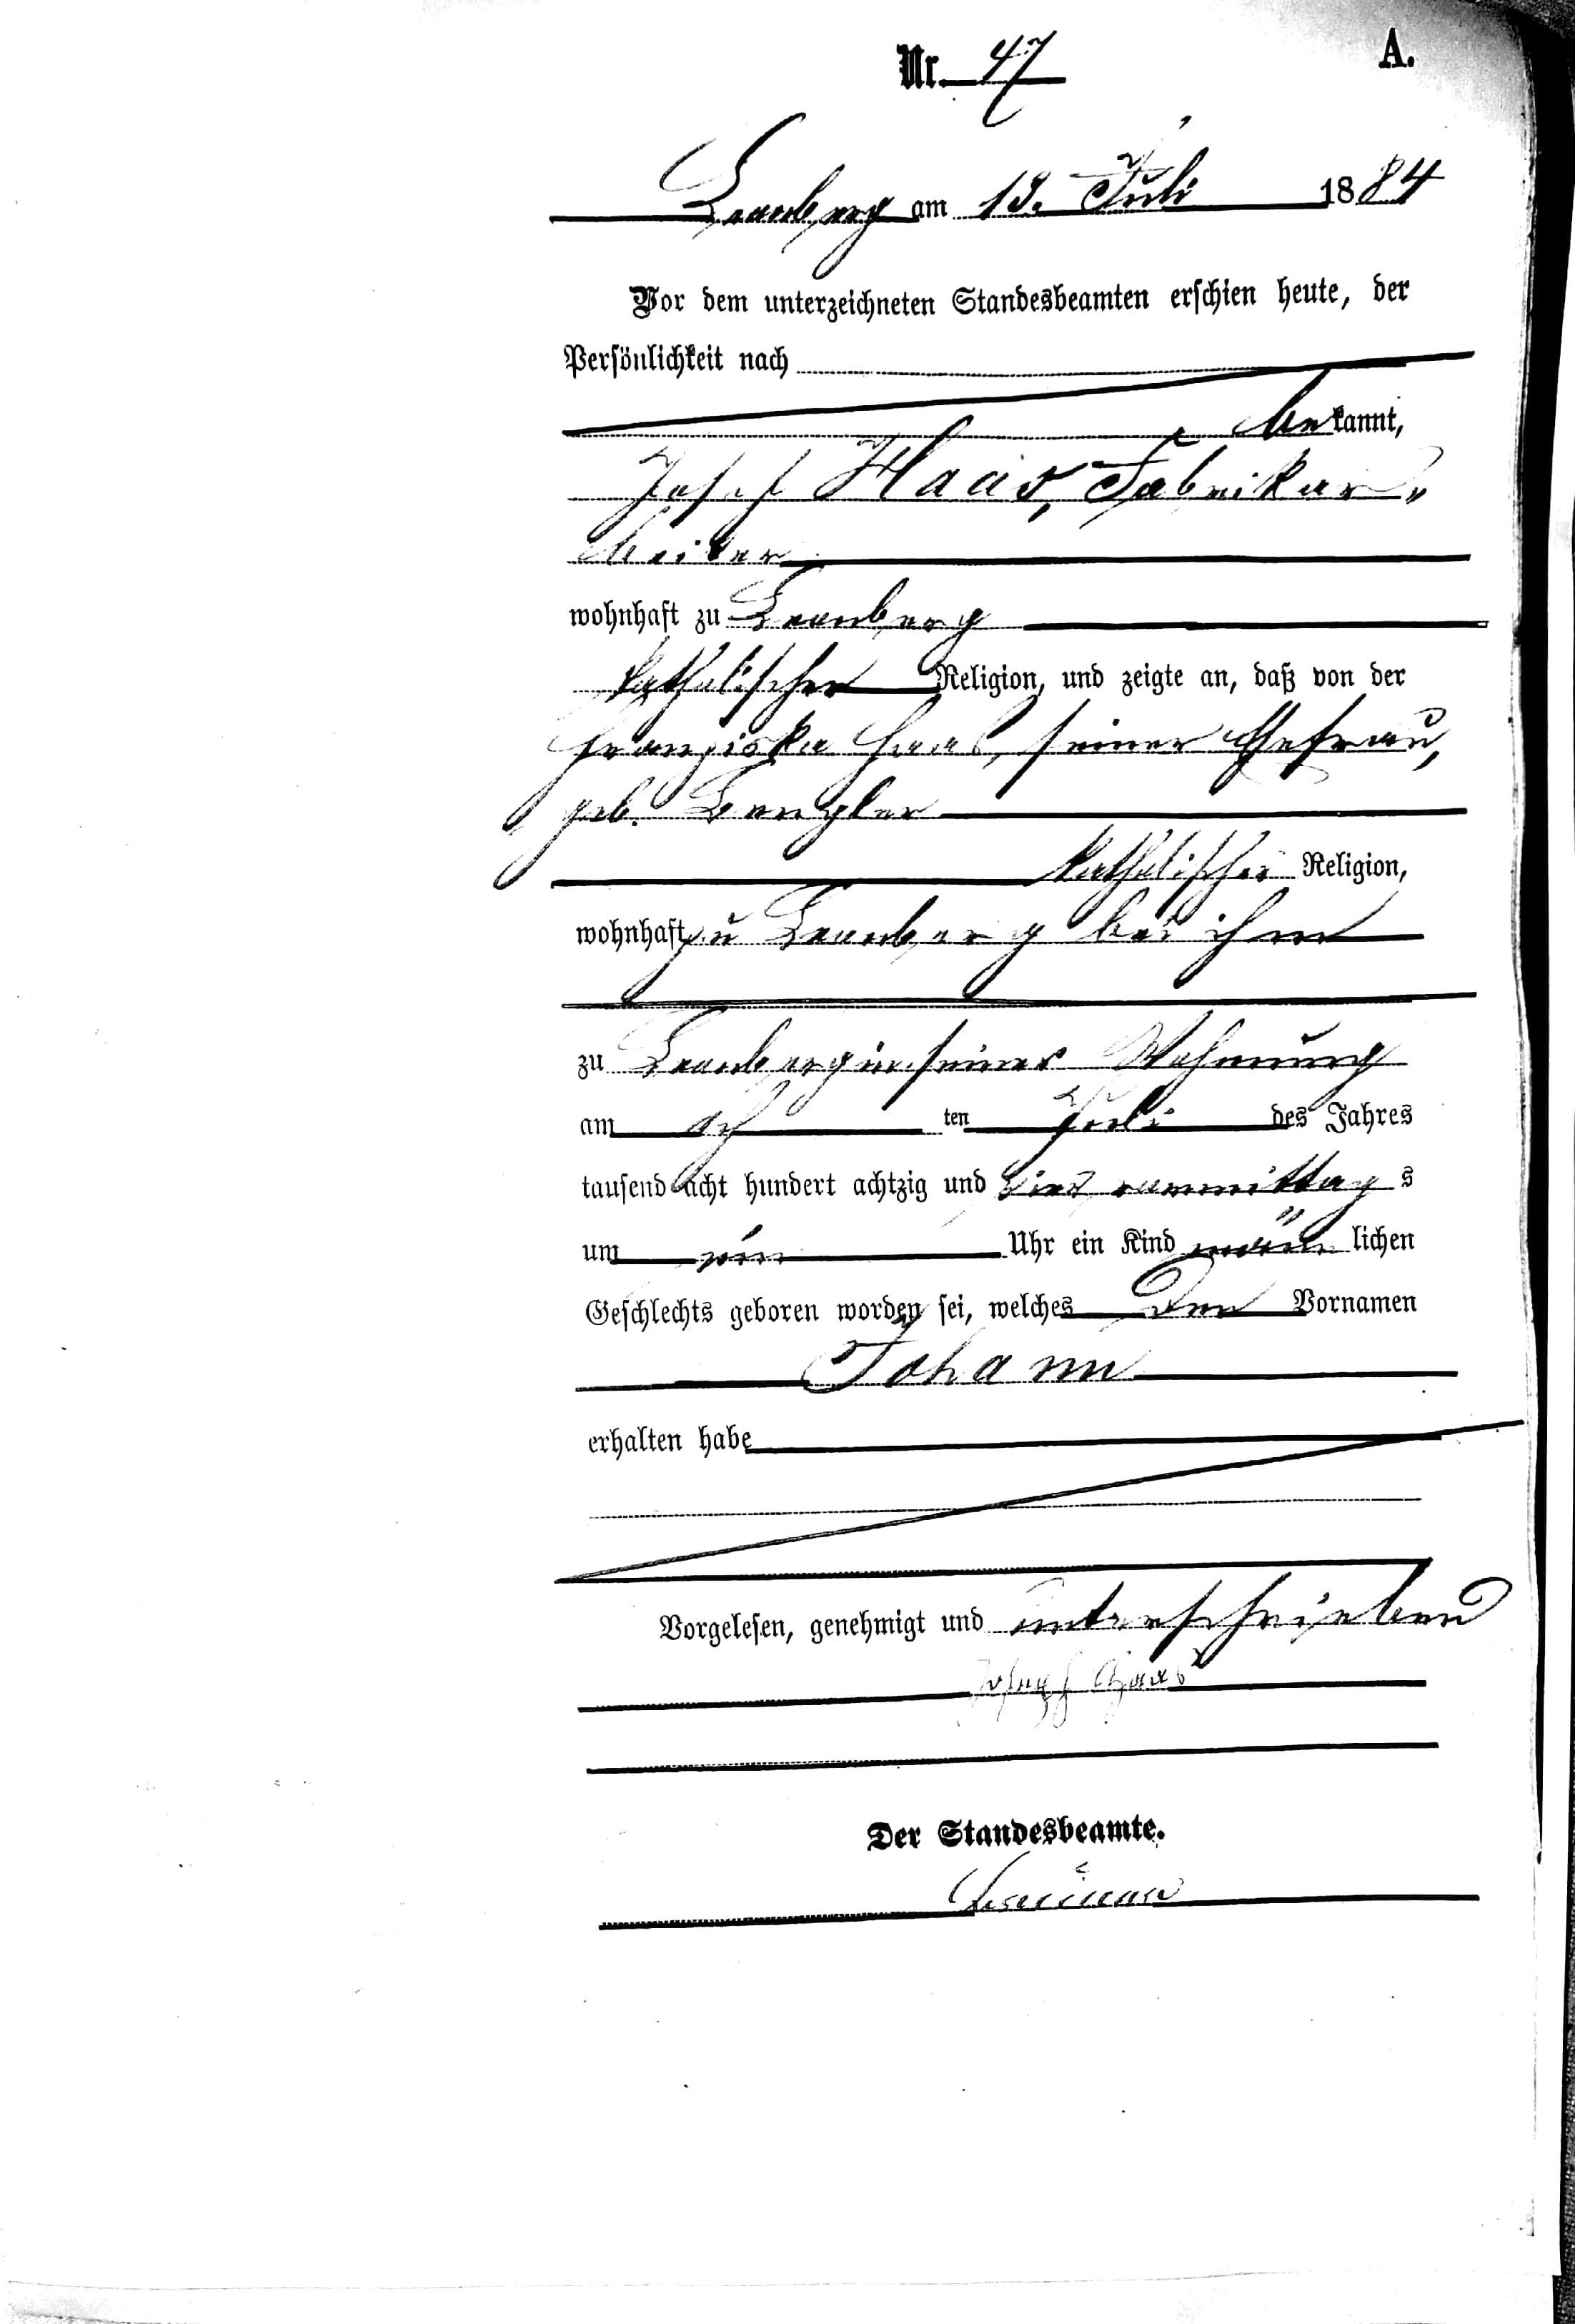
\includegraphics[width=0.85\linewidth,height=\textheight,keepaspectratio,alt={Eintrag Nr. 47 im Geburtenregister des Standesamts Leonberg vom 13. Juli 1884: Der Fabrikarbeiter Josef Haas zeigt die Geburt seines Sohnes Johann am 11. Juli, nachmittags um fünf Uhr, an und unterschreibt den Eintrag eigenhändig.}]{imagens/doc_haas_nascimento_johann_1884.jpg}
\caption{Eintrag Nr. 47 im Geburtenregister des Standesamts Leonberg vom
13. Juli 1884: Der Fabrikarbeiter Josef Haas\index[pessoas]{haas, josef@Haas, Josef} zeigt die Geburt seines
Sohnes Johann am 11. Juli, nachmittags um fünf Uhr, an und unterschreibt
den Eintrag eigenhändig.}
\end{figure}

Es gab eine Unklarheit, die dieses Papier beseitigte. In Agenors
Tabelle, die jahrelang unsere beste Quelle war, ist Johann am „8. Juli``
geboren. Der Eintrag sagt den elften. Der Unterschied beträgt drei Tage
und mag klein erscheinen, aber für einen Forscher ist er alles: Eines
der beiden Daten ist richtig und das andere falsch, und nur das
Originaldokument entscheidet. Agenor\index[pessoas]{haas, agenor@Haas, Agenor}, der Ingenieur ist, weiß besser als
jeder andere, dass eine überprüfte Messung mehr wert ist als eine
notierte; in diesem Buch gilt das Standesamtsregister, und der Fata\index[pessoas]{haas, johann@Haas, Johann} hat
am 11. Geburtstag. Er starb 1969, ohne zu ahnen, dass es diese Frage
einmal geben würde. Ich glaube, er hätte darüber gelacht.

\section{Die Unterschrift}\label{die-unterschrift}

Bei dieser Unterschrift muss ich einen Moment verweilen, denn sie war
es, die mich aus der Fassung brachte.

Ein Meteorologe hat sein Leben lang mit indirekten Zeichen zu tun. Wir
sehen den Wind nicht: Wir sehen, was er mit einem Anemometer macht. Wir
sehen die Kaltfront nicht: Wir sehen den Temperatursprung in einer
Kurve. Fast alles, was wir über die Atmosphäre wissen, stammt aus
Spuren. Und jahrelang war auch alles, was ich über die Haas in
Deutschland wusste, nur Spur: der Name in einer Schiffsliste, ausgefüllt
von einem französischen Schreiber; der Name in einer Tabelle, eingetippt
von einem Cousin; der Name in einem Taufeintrag aus Stoffen\index[lugares]{stoffen@Stoffen}, geschrieben
von einem Pfarrer, und der war nicht einmal der unsere. Immer die Hand
eines anderen.

Die Unterschrift von Josef Haas\index[pessoas]{haas, josef@Haas, Josef} war in diesem ganzen Stapel das Erste,
was ein Haas aus Bayern\index[lugares]{bayern@Bayern} mit eigener Hand geschrieben hatte. Kein Eintrag
über ihn: eine Geste von ihm. An einem Julitag 1884 nahm ein
siebenunddreißigjähriger Arbeiter, die Hände wahrscheinlich gezeichnet
von der Arbeit im Werk, eine Stahlfeder und zeichnete seinen eigenen
Namen auf ein amtliches Blatt, um dem Staat zu sagen, dass ihm ein Sohn
geboren war. Dieser Sohn sollte mein Großvater werden. Die Feder
zitterte ein wenig. Die Tinte verlief bei einem Buchstaben. Und das
Papier bewahrte all das hundertvierunddreißig Jahre lang.

Ich erlaube mir hier eine nachgestellte Szene, und ihr wisst: Wenn ich
das tue, ist es Vorstellung, die sich auf ein Dokument stützt.

\emph{Leonberg\index[lugares]{leonberg@Leonberg}, Oberpfalz\index[lugares]{oberpfalz@Oberpfalz}, 13. Juli 1884.} Josef Haas\index[pessoas]{haas, josef@Haas, Josef} verlässt an einem
Sommersonntag das Haus. Vor zwei Tagen hat Franziska entbunden, an einem
Freitag um fünf Uhr nachmittags, und das Gesetz schreibt vor, die Geburt
beim Standesbeamten anzuzeigen. Er trägt, stelle ich mir vor, die am
wenigsten abgetragene Kleidung, die er hat. Der Beamte kennt ihn; der
Eintrag sagt \emph{der Persönlichkeit nach bekannt}, was bedeutet, dass
Josef keine Zeugen brauchte, um zu beweisen, wer er war. Leonberg\index[lugares]{leonberg@Leonberg} ist
klein, und einen Arbeiter aus dem Werk kennt man. Der Beamte füllt das
Formular aus und fragt nach dem Namen des Kindes. „Johann``, sagt Josef.
Es ist ein gewöhnlicher Name, der gewöhnlichste von allen im
katholischen Bayern\index[lugares]{bayern@Bayern}, der Name des Täufers und des Evangelisten. Der
Beamte schreibt. Er liest den Eintrag laut vor. Josef sagt, es sei
richtig, und unterschreibt.

Ich weiß nicht, ob es so war. Ich weiß, dass es so hätte sein können und
dass das Wesentliche auf dem Papier steht: der Tag, die Stunde, die
Namen, die Unterschrift.

Beim Anblick dieser Schrift denke ich an all die Papiere, die Johann
später unterschreiben würde. Die Heirat in Eibenstock\index[lugares]{eibenstock@Eibenstock} 1907. Irgendein
Einschiffungsdokument in Marseille\index[lugares]{marseille@Marseille} 1913. Die Urkunde über Lote 17 in Rio
do Ouro, zusammen mit dem Freund, mit dem er das Land kaufte. Die
Verträge für die Bauten in Ituporanga\index[lugares]{ituporanga@Ituporanga}: die Hauptkirche, das Pfarrhaus,
das Franziskanerseminar, den Erweiterungsbau des
Schwesternkrankenhauses. Keines dieser Papiere habe ich. Aber plötzlich
wusste ich, wie die Schrift seines Vaters ausgesehen hatte. Und ich
dachte an meine eigene Unterschrift, die ihr von den Schulzeugnissen
kennt, von den Einverständniserklärungen für Ausflüge, von den
Vollmachten. Alles hängt an ein und derselben Hand, die nach und nach
den Besitzer wechselt.

\section{Das zweite Blatt}\label{das-zweite-blatt}

Johanns Eintrag war das, wonach ich gesucht hatte. Das zweite Blatt war
das, was ich fand.

Bei Recherchen auf einem deutschen Standesamt durchsucht das System der
Stadtverwaltung die Register nach dem Familiennamen. Und unter den
Treffern jenes Morgens erschien ein lebender Mensch: ein Haas, 1941 in
Leonberg\index[lugares]{leonberg@Leonberg} geboren, wohnhaft in Maxhütte-Haidhof\index[lugares]{maxhutte-haidhof@Maxhütte-Haidhof}.

Ich will hier vorsichtig sein, und ich erkläre, warum. Diesen Mann gibt
es: Er ist ein Mensch aus Fleisch und Blut, der, als ich dort war,
Anfang siebzig war, in derselben Stadt wohnte, in der der Fata\index[pessoas]{haas, johann@Haas, Johann} geboren
wurde, und nicht wusste (oder, wenn er es wusste, nichts von mir
wusste), dass ein Nachkomme des ausgewanderten Sohnes von Josef Haas\index[pessoas]{haas, josef@Haas, Josef} mit
einem Stammbaum in der Hand in derselben Stadt stand. Er hat ein Recht
auf seine Privatsphäre, und das europäische Recht schützt dieses Recht,
vom Anstand ganz abgesehen. Deshalb nennt dieses Buch weder seinen Namen
noch seine Straße noch irgendetwas, womit man ihn finden könnte. Und
dieses Buch erzählt von keiner Begegnung mit ihm. Es würde davon
erzählen, wenn es etwas zu erzählen gäbe.

Ein Haas, 1941 in Leonberg\index[lugares]{leonberg@Leonberg} geboren. Mitten im Krieg. Im selben Jahr, in
dem auf der anderen Seite der Welt Brasilien mit Deutschland brach und
der Fata\index[pessoas]{haas, johann@Haas, Johann} im Alto Vale do Itajaí\index[lugares]{itajai@Itajaí} die geladene Flinte in Reichweite hielt
und im Keller Radio hörte, während ein Enkel die Straße im Auge behielt.
Während die Familie in Santa Catarina lernte, Angst davor zu haben,
Deutsch zu sprechen, wurde in Leonberg\index[lugares]{leonberg@Leonberg} ein Kind mit demselben
Familiennamen geboren, in einem Deutschland, das bombardiert, besetzt
und geteilt werden sollte. Die beiden Hälften der Familie erlebten
denselben Krieg auf entgegengesetzten Seiten des Ozeans, ohne
voneinander zu wissen. Der Text zum Hundertjahrfeier erzählt, dass João
und Maria 1945 Kleidung und Lebensmittel in das zerstörte Deutschland
schickten, ohne zu wissen, ob sie dort noch lebende Verwandte hatten,
„wenn sie überhaupt noch welche hatten``. Vielleicht hatten sie welche:
In Leonberg\index[lugares]{leonberg@Leonberg} gab es einen vierjährigen Jungen mit demselben
Familiennamen.

Ich weiß nicht, in welchem Grad er mit uns verwandt ist. Johann hatte
Geschwister: Josef, Alois, Georg, Maria, Franziska, Therese. Die Männer
gaben den Familiennamen weiter. Wenn dieser Haas von 1941 der Enkel
eines von ihnen ist, dann war sein Vater ein Cousin ersten Grades meines
Vaters, Opa Baldoíno, und er ist mein Cousin zweiten Grades. Und eurer,
noch entfernter, aber ein Cousin. Es kann auch ganz anders sein. Haas
ist in Deutschland kein seltener Name, und ein Namensvetter in einer
Arbeiterstadt wäre durchaus möglich. Ein ehrlicher Forscher darf die
Verwandtschaft ohne Dokument nicht behaupten, und ich habe das Dokument
nicht. Ich habe die Übereinstimmung des Ortes, die stark ist, und die
Übereinstimmung des Namens, die schwach ist.

Dazu kommt die Falle der gleichnamigen Orte, von der ich in Kapitel 2
gesprochen habe. Es gibt ein viel bekannteres Leonberg\index[lugares]{leonberg@Leonberg} als unseres, bei
Stuttgart in Württemberg, und es gibt dort auch ein Heumaden\index[lugares]{heumaden@Heumaden}, heute ein
Stadtteil von Stuttgart. Lange Zeit landete jeder, der unsere Namen auf
der Karte suchte, zuerst an diesen Orten, Hunderte von Kilometern vom
richtigen entfernt. Ein Meteorologe kennt diese Art Fehler: Es ist der
einer Station mit vertauschten Koordinaten, die einen richtigen Wert vom
falschen Ort meldet und die ganze Karte verdirbt. Deshalb genügt mir ein
gleicher Familienname in einer Stadt gleichen Namens nicht. Aber hier
ist keine Verwechslung des Ortes möglich: Es war das Leonberg\index[lugares]{leonberg@Leonberg} des
Eintrags Nr. 47, das Leonberg\index[lugares]{leonberg@Leonberg} in der Oberpfalz\index[lugares]{oberpfalz@Oberpfalz}, dasselbe, in dem Josef
1884 unterschrieben hatte. Wenn es eine Unklarheit gibt, dann liegt sie
allein im Blut.

Es gibt eine Komplikation, und ich halte sie fest, weil sie zur
Geschichte gehört. Auf derselben Reise suchte ich das Haus. Peter, mit
dem ich sprach, sagte, der Cousin meines Vaters lebe. Die Nachbarn des
Hauses, zu dem ich kam, sagten etwas anderes: Der gleichnamige Haas sei
gestorben, und seine Töchter wohnten in Österreich. Vielleicht habe ich
am falschen Haus geklopft. Vielleicht sprachen die beiden von
verschiedenen Personen. Ich habe das dort nicht geklärt, und ich werde
es hier nicht mit Vermutungen klären.

Und es gibt ein Schweigen, das ich jetzt anders verstehe. Der Fata\index[pessoas]{haas, johann@Haas, Johann}
sprach nicht von den lebenden Verwandten in Deutschland. Aber die
Familie bewahrte Briefe auf, die von dort kamen, von einer Adresse im
Vogtland\index[lugares]{vogtland@Vogtland} in Sachsen\index[lugares]{sachsen@Sachsen}. Jemand auf der anderen Seite wusste von uns.

An jenem Morgen dachte ich nicht wie ein Forscher. Ich dachte wie ein
Enkel. Was ich fühlte, ist, so stelle ich mir vor, was ein
Schiffbrüchiger fühlt, der nach vielen Tagen Rauch auf einer Insel
sieht. Es ist nicht die Rettung. Es ist der Beweis, dass dort Menschen
sind.

Während der ganzen Forschung, seit dem Tisch in Vidal Ramos\index[lugares]{vidal ramos@Vidal Ramos} im Jahr
2012, war es diese Frage, die das Buch antrieb: \emph{Ist auf der
anderen Seite noch jemand?} Der Fata\index[pessoas]{haas, johann@Haas, Johann} starb 1969 in dem Glauben, nein.
Ich glaubte, die Mota\index[pessoas]{meier, maria@Meier, Maria} sei 1973 gestorben, ohne dass jemand auf der
anderen Seite davon erfuhr. Erst 2026, mit den Briefen aus Rempesgrün\index[lugares]{rempesgrun@Rempesgrün} in
Kapitel 7, entdeckte ich, dass ihre Verwandten in Sachsen\index[lugares]{sachsen@Sachsen} davon erfahren
und ihr Beileid geschickt hatten. Die den Faden hatten fallen lassen,
waren wir. Und da war nun, auf dem Bildschirm einer Stadtverwaltung in
der Oberpfalz\index[lugares]{oberpfalz@Oberpfalz}, das Ende des Fadens auf der anderen Seite.

Ich schreibe diese Seiten also auch als einen möglichen Brief. Sollte
dieses Buch eines Tages, übersetzt oder nicht, zu einem Haas gelangen,
der 1941 in Leonberg\index[lugares]{leonberg@Leonberg} geboren wurde, dann soll er wissen, dass 1913 ein
junger Mann namens Johann, Sohn des Arbeiters Josef und der Franziska
Dengler, von dort aufbrach und mit seiner Frau und zwei kleinen Kindern
nach Brasilien ging; dass dieser junge Mann an einem Ort namens
Ituporanga\index[lugares]{ituporanga@Ituporanga} Kirchen und Grabmäler gebaut hat; dass er zwölf Kinder hatte,
von denen sieben erwachsen wurden; dass seine Nachkommen heute mehr als
sechshundert sind; und dass einer dieser Nachkommen an einem
Februarmorgen in der Regensburger Straße war und erfuhr, dass es ihn
gibt. Die Tür bleibt offen. Ich weiß nicht, ob jemand anklopfen wird.

\section{Der Ballon durchstößt die
Wolke}\label{der-ballon-durchstuxf6uxdft-die-wolke}

Es gibt einen Moment im Leben eines Meteorologen, der nie aufhört, schön
zu sein: den Start einer Radiosonde. Ein Latexballon, mit Wasserstoff
oder Helium gefüllt, an dem ein kleines Kästchen mit Sensoren hängt,
steigt von der Station auf und beginnt, Druck, Temperatur und Feuchte zu
senden. Auf dem Bildschirm zeichnet sich das Profil von unten nach oben.
Eine Zeit lang sind die Zahlen vorhersehbar: Die Temperatur fällt, die
Feuchte schwankt. Und dann tritt der Ballon plötzlich in eine Wolke ein,
die Feuchte geht auf hundert Prozent, die Temperaturkurve knickt, und
man weiß, dass er jetzt drinnen ist, mitten im Weiß, ohne etwas zu
sehen. Und dann, noch plötzlicher, tritt er oben heraus, die Feuchte
stürzt ab, die Luft wird trocken und klar, und der Ballon steigt weiter
in einen Himmel, den von unten niemand sah.

Die ganze Forschung seit 2012 war der Ballon in der Wolke gewesen.
Namen, die nicht zusammenpassten, abweichende Daten, gleichnamige Orte,
eine Tabelle mit Lücken, eine Schiffsliste mit einem falschen Alter, ein
„Leonberg\index[lugares]{leonberg@Leonberg}``, das ein anderes Leonberg sein konnte, ein „Sandberg\index[lugares]{sandberg@Sandberg}``, das
ich auf der Karte nicht fand. Feuchte hundert Prozent. Und der Eintrag
Nr. 47 war der Moment, in dem der Ballon oben herauskam. Von einem
Augenblick auf den anderen wurde die Luft klar. Johann Haas\index[pessoas]{haas, johann@Haas, Johann}, geboren am
11. Juli 1884, um fünf Uhr nachmittags, in Leonberg\index[lugares]{leonberg@Leonberg}. Sohn von Josef
Haas, Fabrikarbeiter, und Franziska Dengler\index[pessoas]{dengler, franziska@Dengler, Franziska}. Väterlicherseits Enkel von
Michael Haas\index[pessoas]{haas, michael@Haas, Michael} und Kunigunde Stadelmann\index[pessoas]{stadelmann, kunigunde@Stadelmann, Kunigunde}, wie ich erst 2026 erfahren
sollte. Eine gerade Linie ohne Wolken, von euch bis zum Rauch von
Sandberg\index[lugares]{sandberg@Sandberg}.

Ich weiß nicht, wie lange wir drinnen waren. Ich werde es nicht
erfinden. Ich weiß, dass ich mit dem Papier hinausging und dass draußen
auf der Straße die Kälte dieselbe war wie vorher, ich aber nicht.

Wenn ich heute an jenen Morgen zurückdenke, denke ich an Opa Baldoíno,
der im Dezember 2013 starb, vier Jahre davor. Er war das zehnte Kind von
Johann, das 1924 auf der Lichtung von Rio Novo\index[lugares]{rio novo@Rio Novo} geboren wurde. Er hätte
dieses Papier gern gesehen. Vielleicht hätte er nichts gesagt, denn die
Männer seiner Generation sagten wenig. Vielleicht wäre er nur langsam
mit dem Finger über die Unterschrift des Großvaters gefahren, den er nie
gekannt hat. Ich denke an Oma Adelina, die in jenem Februar noch lebte,
in Vidal Ramos\index[lugares]{vidal ramos@Vidal Ramos}. Ich denke an euch beide, die das eines Tages lesen
würden.

Und ich denke schließlich an das, was dieses Papier noch nicht sagte: Es
fehlte die Hälfte. Der Eintrag Nr. 47 gab mir den Fata\index[pessoas]{haas, johann@Haas, Johann} ganz, mit Vater,
Mutter, Großvater und Dorf. Aber der Fata\index[pessoas]{haas, johann@Haas, Johann} war nie allein. Neben ihm, in
der Schiffsliste, auf dem Abschiedsfoto, im Grab von Aurora\index[lugares]{aurora@Aurora}, war immer
sie. Das Mädchen, das um zwei Uhr nachts in einem hügeligen Dorf nahe
Böhmen geboren wurde und dessen Namen die Familie ein Jahrhundert lang
wiederholte wie jemand, der ein Gebet aufsagt, ohne die Worte zu
verstehen.

Es fehlte die andere Hälfte: die Mota\index[pessoas]{meier, maria@Meier, Maria}. Es fehlte Heumaden\index[lugares]{heumaden@Heumaden}.

\section{Für euch zum Entdecken}\label{fuxfcr-euch-zum-entdecken-16}

\begin{itemize}
\tightlist
\item
  In welchem Verwandtschaftsgrad, wenn überhaupt, steht der 1941 in
  Leonberg\index[lugares]{leonberg@Leonberg} geborene Haas zu Josef Haas\index[pessoas]{haas, josef@Haas, Josef}? Wenn er der Enkel eines Bruders
  von Johann ist, von welchem: Josef, Alois oder Georg?
\item
  Wer hatte recht: Peter, der sagte, der Cousin meines Vaters lebe, oder
  die Nachbarn, die sagten, der gleichnamige Haas sei gestorben und
  seine Töchter wohnten in Österreich? Habe ich am falschen Haus
  geklopft?
\item
  Wer auf der anderen Seite hat die Briefe aus dem Vogtland\index[lugares]{vogtland@Vogtland} geschrieben,
  und was steht darin? Fragt die Ältesten der Familie, wo diese Briefe
  sind.
\item
  Von wem hat Johann das Arbeiten mit Gips gelernt, wenn der Text zum
  Hundertjahrfeier sagt, er sei „aus einer Familie von Maurern
  gekommen``, und sein Vater Arbeiter im Hüttenwerk war? Von den
  Dengler, von Josefs älteren Brüdern oder von niemandem aus der
  Familie?
\end{itemize}

\chapter{Die Straße nach Heumaden und die Kurrentschrift von
Moosbach\index[lugares]{moosbach@Moosbach}}\label{cap-18}

\emph{49,6° N · 12,4° E, Moosbach\index[lugares]{moosbach@Moosbach}, Oberpfalz\index[lugares]{oberpfalz@Oberpfalz} (Heumaden\index[lugares]{heumaden@Heumaden}, Rückersrieth\index[lugares]{ruckersrieth@Rückersrieth},
Burgtreswitz\index[lugares]{burgtreswitz@Burgtreswitz})}

\begin{quote}
\emph{Die Tinte eines Dorfpfarrers hält länger als das Dorf, das er
kannte.}
\end{quote}

Eine Seite aus einem bayerischen Pfarrbuch widerspricht, so wie ich sie
lese, dem, was die Familie über die Taufe der Mota\index[pessoas]{meier, maria@Meier, Maria} aufgeschrieben hat:
dem Tag und dem Namen der Patin. Eine andere trägt einen Familiennamen,
der nachträglich ausgebessert zu sein scheint. Dieses Kapitel handelt
von vier Seiten.

\section{Eine Straße, die man zuerst auf der Karte
abfährt}\label{eine-strauxdfe-die-man-zuerst-auf-der-karte-abfuxe4hrt}

Heumaden\index[lugares]{heumaden@Heumaden} liegt in Luftlinie etwa fünfzig Kilometer nordöstlich von
Maxhütte-Haidhof\index[lugares]{maxhutte-haidhof@Maxhütte-Haidhof}, fast auf demselben Längengrad, ein Stück näher an der
tschechischen Grenze. Es ist eines jener Dörfer, die auf der Landkarte
in ein Komma passen: eine Handvoll Dächer, eine Nebenstraße, Felder
ringsum, dunkle Flecken Wald. Heute gehört es zum Markt Moosbach\index[lugares]{moosbach@Moosbach} im
Landkreis Neustadt an der Waldnaab in der Oberpfalz\index[lugares]{oberpfalz@Oberpfalz}. Die Pfarrei ist
St.~Peter und Paul in der Mitte von Moosbach\index[lugares]{moosbach@Moosbach}. Ringsum, nur wenige
Kilometer voneinander entfernt, liegen die übrigen Namen dieser
Geschichte: Rückersrieth\index[lugares]{ruckersrieth@Rückersrieth}, wo euer Ururgroßvater Georg Adam Meier\index[pessoas]{meier, georg adam@Meier, Georg Adam} geboren
wurde, und Burgtreswitz\index[lugares]{burgtreswitz@Burgtreswitz}, wo eure Ururgroßmutter Franziska Voit\index[pessoas]{voit, franziska@Voit, Franziska} geboren
wurde, ein Dorf, das die Burg im Namen trägt, weil es tatsächlich eine
hat.

Das erste Mal bin ich diese Straße auf der Karte gefahren, und so möchte
ich auch beginnen, denn wahrscheinlich werdet ihr sie ebenso fahren. Ich
öffnete das Satellitenbild und zoomte langsam heran. Erst Europa, dann
Deutschland, dann Bayern\index[lugares]{bayern@Bayern}, dann jene Gegend mit niedrigen Hügeln und
Wäldern zwischen Donau und Böhmen, der Oberpfälzer Wald. Dann Moosbach\index[lugares]{moosbach@Moosbach}
mit seiner Kirche. Dann, im Nordosten, Heumaden\index[lugares]{heumaden@Heumaden}. Ein paar Häuser, eine
Straße, Felder in langen Streifen, das alte Erbe der mittelalterlichen
Flurordnung. Lange habe ich auf diese Streifen geschaut. Auf einem davon
hat die Mota\index[pessoas]{meier, maria@Meier, Maria} vielleicht als junges Mädchen Kühe gemolken, bevor sie
heiratete und fortging. Im Text zur Hundertjahrfeier heißt es, Maria
habe „für Lohn Kühe gemolken''. Sie sei es gewesen, schreibt Marise\index[pessoas]{lourenco, marise haas@Lourenço, Marise Haas},
„die sich mit der Feldarbeit auskannte''.

Schon der Name des Dorfes scheint vom Land zu sprechen. \emph{Heu} ist
Heu, \emph{Mahd} ist das Mähen des Grases mit der Sense. Ich bin kein
Sprachwissenschaftler und will auf diese Herkunft nicht schwören, aber
es fällt schwer, in \emph{Heumaden\index[lugares]{heumaden@Heumaden}} nicht so etwas wie „die Heuwiesen''
zu hören, „den Ort, an dem gemäht wird''. Ein Dorf der Weiden und der
Kühe. Es passt, dass die Mota\index[pessoas]{meier, maria@Meier, Maria} mit dem Melken aufwuchs. Und es passt
auch, was mir erst später auffiel, dass sie ihr Alter in Ribeirão das
Pacas im Alto Vale do Itajaí\index[lugares]{itajai@Itajaí} verbrachte, mit Tieren und Äckern
beschäftigt, auf die Holzstöcke gestützt, an die sich die Enkel
erinnern. In Marises Text steht, dass sie in der Nähe ihrer Tochter
Maria weiter „den Boden umgrub, ihre Pflanzen zog und ihre Tiere
hielt''.

Für einen Meteorologen hat diese Gegend noch ein weiteres Merkmal: Sie
liegt auf der Innenseite des Kontinents. Weit vom Meer entfernt hat die
Oberpfalz\index[lugares]{oberpfalz@Oberpfalz} kältere Winter und heißere Sommer als der Westen Deutschlands,
und der Wind aus dem Osten, aus Böhmen, kommt trocken und schneidend an.
Die Alten hatten einen Namen für ihn. Die Mota\index[pessoas]{meier, maria@Meier, Maria} wuchs in diesem Klima
großer Gegensätze auf, mit langem Frost und kurzem Sommer, und landete
an einem Ort, wo die Feuchtigkeit nie nachlässt und der Winter eine
Jahreszeit von wenigen Wochen ist. Ich weiß nicht, was ihr Körper von
diesem Tausch hielt. Ich weiß, dass sie fünfundachtzig Jahre alt wurde.

Die Pfarrbücher von Moosbach\index[lugares]{moosbach@Moosbach} liegen heute im Bischöflichen Zentralarchiv
Regensburg\index[lugares]{regensburg@Regensburg}. Sie wurden digitalisiert und sind über das Portal Matricula
für jeden zugänglich, das Kirchenbücher aus halb Europa zusammenführt.
Nach diesen Digitalisaten zitiere ich die Seiten (das Taufbuch von 1847
bis 1904, das Trauungsbuch von 1853 bis 1935), denn mit ihnen könnt ihr,
oder jeder Vetter und jede Base, jede Zeile nachprüfen, die ich hier
abschreibe. Gleich in welchem Raum, an welchem Tisch oder vor welchem
Bildschirm man ein solches Buch aufschlägt, die Erfahrung ist dieselbe:
eine alte Seite, eine Schrift, die man nicht versteht, und die Hoffnung,
irgendwo darin einen bekannten Namen zu finden.

\section{Die Schrift, die die Mota lesen
konnte}\label{die-schrift-die-die-mota-lesen-konnte}

Das Erste, was ein Brasilianer vor einem bayerischen Pfarrbuch des 19.
Jahrhunderts entdeckt, ist, dass er nicht lesen kann.

Das Problem ist die Schrift. Die Pfarrer und Schreiber jener Zeit
schrieben in \emph{Kurrentschrift}, der deutschen Schreibschrift, die
jahrhundertelang die gewöhnliche Handschrift im deutschen Sprachraum
war, bis man sie Mitte des 20. Jahrhunderts aufgab. Sie ähnelt nichts,
was wir in der Schule gelernt haben. Das „e'' besteht aus zwei fast
gleichen senkrechten Strichen, wie ein zusammengedrücktes „n''. Das „h''
hängt wie ein Schwanz unter die Zeile. Das „s'' hat zwei Formen, eine
lange in der Wortmitte und eine runde am Ende. Das „r'' sieht aus wie
ein kleines „w''. Das große „M'', das ich vor allem anderen finden
musste, weil es der Anfangsbuchstabe von Meier war, ist eine Folge von
Bögen, die auf den ersten Blick alles Mögliche sein könnte.

Die Mota\index[pessoas]{meier, maria@Meier, Maria} konnte diese Schrift lesen. Der Fata\index[pessoas]{haas, johann@Haas, Johann} auch. Sie hatten in den
bayerischen Schulen so schreiben gelernt, und der Text zur
Hundertjahrfeier erzählt, dass sie Leser waren, dass sie Bücher aus
Deutschland mitbrachten und später Zeitungen aus Blumenau\index[lugares]{blumenau@Blumenau} bezogen, die
zu Beginn des 20. Jahrhunderts noch in Fraktur gedruckt wurden. Ihre
Kinder, in Brasilien geboren, kamen in die Schule und sprachen nur
Deutsch, lernten aber im lateinischen Alphabet zu schreiben, auf
Portugiesisch. Ich, der Enkel, brauchte Tabellen, Beispiele und viel
Geduld, um den Namen meiner Großmutter auf einer Seite zu erkennen, die
in genau der Schrift geschrieben war, in der sie selbst ihre Briefe
schrieb. Das ist eine der greifbarsten Formen der zum Schweigen
gebrachten Sprache, von der ich in Kapitel 7 erzählt habe: Verloren ging
die Sprache, und verloren ging die Hand.

Ich lernte langsam. Zuerst die einzelnen Buchstaben, dann die
Abkürzungen. Die Pfarrer kürzten alles ab: \emph{Gg.} für Georg,
\emph{Kath.} für Katharina, \emph{Mich.} für Michael, \emph{Joh.} für
Johann, \emph{k.} oder \emph{kath.} für katholisch. Sie setzten
Anführungszeichen als Wiederholungszeichen für das, was in der Zeile
darüber stand. Sie mischten Latein ins Deutsche: \emph{et} für „und'',
\emph{Procl.} für die kirchlichen Proklamationen, \emph{idem} für
denselben Pfarrer. Und sie schrieben die Zahlen auf eine Weise, die
einem Meteorologen, der ans Lesen von Tabellen gewöhnt ist, fast
vertraut vorkam.

Die Taufbücher von Moosbach\index[lugares]{moosbach@Moosbach} sind Tabellen. Jede Zeile ist ein Kind. Die
Spalten enthalten von links nach rechts die Nummer des Eintrags, den
Namen des Kindes, die Hebamme, den Vater und seinen Stand, den Wohnort,
die Mutter und ihren Stand, die Herkunft der Mutter, Tag und Stunde der
Geburt, den Tauftag, den Pfarrer, die Paten. Jede Doppelseite enthält
nur wenige Einträge, jedes Jahr einige Dutzend. Um Maria Meier\index[pessoas]{meier, maria@Meier, Maria} zu
finden, kannte ich Jahr und Monat. April 1888. Ich musste nur bis
dorthin blättern.

\section{Seite 441, Eintrag Nr. 36}\label{seite-441-eintrag-nr.-36}

Da stand sie.

Auf Seite 441 des Taufbuchs, zwischen einem Mädchen namens Josefa aus
einer Moosbacher Familie, am Tag zuvor geboren, und einem Jungen namens
Bergmann, am selben Tag wie sie geboren: der Eintrag Nummer 36. In der
Namensspalte, auf zwei Zeilen, zuerst der Familienname, wie es damals
üblich war: \emph{Meier}, dann \emph{Maria}.

Ich lese die Zeile mit euch, Spalte für Spalte, so wie ich sie gelesen
habe.

Hebamme: zwei kleine Gänsefüßchen. \emph{Idem}. Um zu erfahren, wer es
war, muss man eine Zeile höher gehen, zum Eintrag 35, dem der kleinen
Josefa, geboren am 6. April um ein Uhr nachts. Dort steht der Name:
\emph{Glas}. Frau Glas, Hebamme in Moosbach\index[lugares]{moosbach@Moosbach}, hatte in der Nacht zum 6.
April eine Geburt begleitet und in der Nacht zum 7. die nächste. Zwei
Nächte hintereinander mit ihrer Tasche durch die Kälte des bayerischen
Frühlings. Als ich mir in Kapitel 4 die Nacht vorstellte, in der die
Mota\index[pessoas]{meier, maria@Meier, Maria} geboren wurde, hatte ich die beiden Gänsefüßchen noch nicht
bemerkt. Jetzt weiß ich, dass Frau Glas in jener Nacht wahrscheinlich
müde war.

Vater: \emph{Gg. Adam Meier}. Stand: \emph{Krämer}. Lange habe ich dort
\emph{Ökonom} gelesen; die zweite Lesung zeigte \emph{Krämer}, und ich
korrigiere es. Wohnort: \emph{Heumaden\index[lugares]{heumaden@Heumaden}}. Mutter: \emph{Franzisca Voit}.
Herkunft der Mutter: \emph{Burgtresw.}, Burgtreswitz\index[lugares]{burgtreswitz@Burgtreswitz}.

Geburt: \emph{7. April, 2 h. morg.}

Taufe: \emph{7. April}.

Patin: \emph{Kath. Reichenberger, Bäuerin v. Burgtresw.}

\begin{ficha}

\textbf{Archivkarte}: Pfarrei St.~Peter und Paul, Moosbach\index[lugares]{moosbach@Moosbach} (Dekanat
Leuchtenberg, Bistum Regensburg\index[lugares]{regensburg@Regensburg}). Taufbuch 1847--1904 (Matricula:
\texttt{Moosbach\index[lugares]{moosbach@Moosbach}\_Leuchtenberg005}), S. 441, Eintrag Nr. 36. Täufling:
Maria Meier\index[pessoas]{meier, maria@Meier, Maria}. Hebamme: Glas (durch „idem'' angegeben, mit Verweis auf den
vorhergehenden Eintrag). Vater: Georg Adam Meier\index[pessoas]{meier, georg adam@Meier, Georg Adam} (\emph{Gg. Adam
Meier}), \emph{Krämer} in Heumaden\index[lugares]{heumaden@Heumaden}. Mutter: Franziska Voit\index[pessoas]{voit, franziska@Voit, Franziska}
(\emph{Franzisca Voit}), gebürtig aus Burgtreswitz\index[lugares]{burgtreswitz@Burgtreswitz}. Geburt: 7. April
1888, 2 Uhr morgens, in Heumaden\index[lugares]{heumaden@Heumaden}. Taufe: 7. April (Datum in der eigenen
Spalte eingetragen, nach unserer Lesung). Patin: \emph{Kath.
Reichenberger, Bäuerin v. Burgtresw.} Bild:
\texttt{imagens/doc1\_maria\_meier\_1888.jpg}.

\end{ficha}

\begin{figure}
\centering
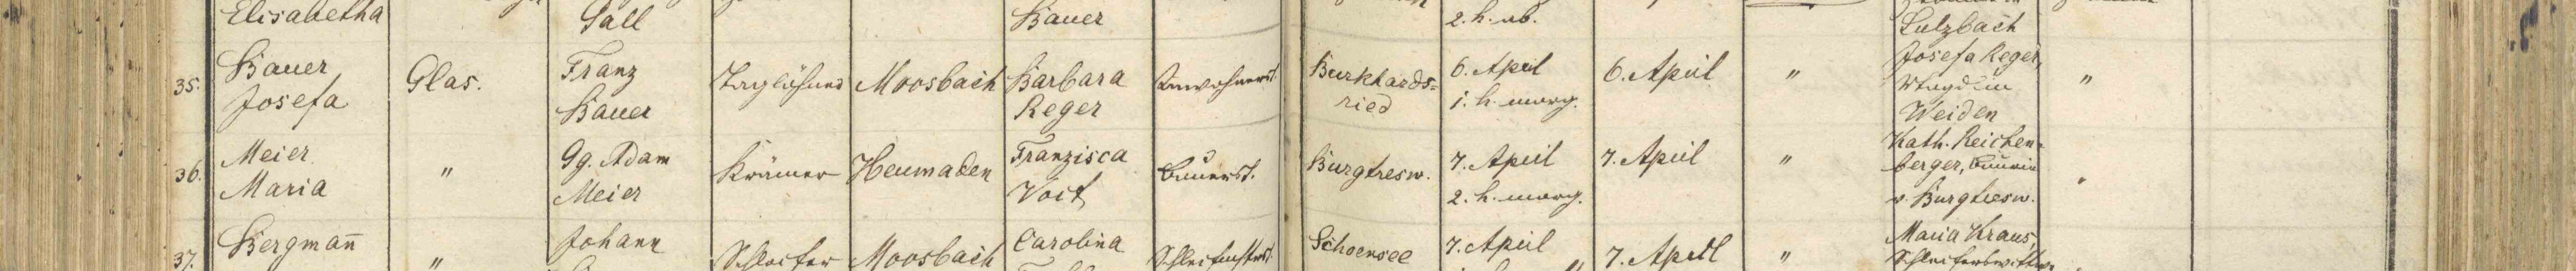
\includegraphics[width=0.85\linewidth,height=\textheight,keepaspectratio,alt={Taufbuch Moosbach, Seite 441: Eintrag Nr. 36, Maria Meier, geboren in Heumaden am 7. April 1888 um zwei Uhr nachts, Tochter von Georg Adam Meier und Franziska Voit; in der Zeile darüber der Name der Hebamme Glas.}]{imagens/doc1_maria_meier_1888.jpg}
\caption{Taufbuch Moosbach, Seite 441: Eintrag Nr. 36, Maria Meier,
geboren in Heumaden\index[lugares]{heumaden@Heumaden} am 7. April 1888 um zwei Uhr nachts, Tochter von
Georg Adam Meier\index[pessoas]{meier, georg adam@Meier, Georg Adam} und Franziska Voit\index[pessoas]{voit, franziska@Voit, Franziska}; in der Zeile darüber der Name der
Hebamme Glas.}
\end{figure}

Ich muss euch etwas erzählen, denn dieses Buch hat eine Regel, und ich
werde sie nicht ausgerechnet in dem Kapitel brechen, in dem sie am
meisten zählt.

In den Aufzeichnungen, die in der Familie kursierten und die ich selbst
an mehr als einer Stelle wiederholt habe, wurde Maria am 8. April
getauft, und Patin war ihre Tante Katharina Meier, Bäuerin in Heumaden\index[lugares]{heumaden@Heumaden}.
Seite 441 sagt, so wie ich sie lese, etwas anderes. Die Taufspalte nennt
den „7. April'', denselben Tag wie die Geburt, was im katholischen
Bayern\index[lugares]{bayern@Bayern} ganz üblich war, wo man rasch taufte, aus Angst, das Kind könnte
ungetauft sterben. Und die Patin heißt Katharina Reichenberger, aus
Burgtreswitz\index[lugares]{burgtreswitz@Burgtreswitz}, dem Dorf der Mutter.

Es gibt eine Vermutung, die beide Fassungen versöhnt, und ich halte sie
als Vermutung fest: Eine Katharina, geborene Meier, Schwester von Georg
Adam, könnte mit einem Reichenberger aus Burgtreswitz\index[lugares]{burgtreswitz@Burgtreswitz} verheiratet
gewesen sein; dann wäre sie zugleich „die Tante Katharina'' der
Überlieferung und die „Kath. Reichenberger'' des Buches. Das wäre schön.
Aber ich habe kein Dokument, das es beweist, und eine schöne Vermutung
ist genau die Art von Dingen, der ein Forscher am meisten misstrauen
sollte. Ich lasse beide Fassungen nebeneinander stehen, so wie ich in
den früheren Kapiteln die beiden Daten von Gertrudes und die beiden
Grabstätten von Luisa\index[pessoas]{haas, luisa@Haas, Luisa} und Walter nebeneinander stehen ließ. Die Wahrheit
über die Patin der Mota\index[pessoas]{meier, maria@Meier, Maria} steht in irgendeinem anderen Buch, in einem
Trauungseintrag aus Burgtreswitz\index[lugares]{burgtreswitz@Burgtreswitz}, den ich noch nicht gelesen habe. Der
bleibt euch, wenn ihr wollt.

Keiner dieser Zweifel nimmt dem Wesentlichen etwas. Am 7. April 1888 um
zwei Uhr nachts wurde in einem Haus in Heumaden\index[lugares]{heumaden@Heumaden} das Mädchen geboren, das
die Mota\index[pessoas]{meier, maria@Meier, Maria} werden sollte. Der Name, den die Familie ein Jahrhundert lang
in Ituporanga\index[lugares]{ituporanga@Ituporanga} und in Aurora\index[lugares]{aurora@Aurora} wiederholt hatte, ohne dass jemand genau
wusste, wo dieser Ort lag, hatte eine Zeile in einem Buch.

Ich erlaube mir noch einmal, mir etwas vorzustellen.

\emph{Moosbach\index[lugares]{moosbach@Moosbach}, Oberpfalz\index[lugares]{oberpfalz@Oberpfalz}, 7. April 1888.} Es ist ein Samstag. Frau Glas
hat das Haus der Meiers noch vor Tagesanbruch verlassen. Später trägt
jemand das Neugeborene zur Kirche St.~Peter und Paul, in Tücher
gewickelt gegen die Aprilkälte. Wahrscheinlich geht die Mutter,
Franziska, nicht mit; Frauen, die gerade entbunden hatten, blieben zu
Hause. Es gehen der Vater, die Patin, vielleicht eine Nachbarin. Der
Pfarrer gießt das Wasser, spricht den Namen. Danach schlägt er in der
Sakristei das große Buch auf und schreibt, in der Schrift, die ich erst
ein Jahrhundert später lesen lernen sollte, die Zeile Nummer 36 jenes
Jahres. Niemand dort ahnt, dass dieses Mädchen am anderen Ende der Welt
sterben wird, mit 85 Jahren, in einem Ort namens Aurora\index[lugares]{aurora@Aurora}, ohne diese
Kirche je wiederzusehen.

\section{Der 23. November 1884}\label{der-23.-november-1884}

Nachdem Maria gefunden war, fügte sich der Rest des Puzzles wie von
selbst. Wenn sie die Tochter von Georg Adam Meier\index[pessoas]{meier, georg adam@Meier, Georg Adam} und Franziska Voit\index[pessoas]{voit, franziska@Voit, Franziska}
war, mussten die beiden einige Jahre zuvor dort geheiratet haben. Das
Trauungsbuch von Moosbach\index[lugares]{moosbach@Moosbach}, das von 1853 bis 1935 reicht, enthält auf
Seite 93 den Eintrag Nummer 20.

Das Datum in der ersten Spalte: \emph{23. Nov.}, der 23. November 1884.
Ein Sonntag.

Bräutigam: \emph{Adam Meier}. Stand: \emph{Wagner}, katholisch. Ein
Wagner war der Handwerker, der Räder und Wagen baute, der Felgen,
Speichen und Naben fertigte und ganze Fuhrwerke, mit denen man die
Felder bestellte. Wohnort: Heumaden\index[lugares]{heumaden@Heumaden}. Eltern: \emph{Mich. Meier et
Margaretha Pfanenstein}, mit nur einem „n'' und einem kleinen Strich
darüber, so wie man den Doppelbuchstaben abkürzte. Familienstand: ledig.
Geboren am: \emph{9. März 1859}.

Braut: \emph{Franzisca Voit}. Stand: \emph{Bauerstochter}, katholisch.
Wohnort: Burgtreswitz\index[lugares]{burgtreswitz@Burgtreswitz}. Eltern: \emph{Joh. Voit et Barbara Woppman}.
Familienstand: ledig. Geboren am: \emph{29. Juni 1861}.

Trauzeugen: \emph{Mich. Meier, Wagner, Heumaden\index[lugares]{heumaden@Heumaden}, et Johan Voit, Bauer,
Burgtreswitz\index[lugares]{burgtreswitz@Burgtreswitz}}. Die beiden Väter. Der Vater des Bräutigams, der Räder
baute, und der Vater der Braut, der den Boden bestellte, standen neben
ihren Kindern vor dem Altar.

Danach das Datum der standesamtlichen Bescheinigung, \emph{8.
Nov.~1884}, denn seit 1876 musste die Ehe auch vor dem Standesamt
geschlossen werden, und die \emph{3 Procl.}, die drei kirchlichen
Aufgebote, die an drei aufeinanderfolgenden Sonntagen in der Messe
verkündet wurden, damit sich melde, wer von einem Ehehindernis wusste.
Niemand meldete sich.

\begin{ficha}

\textbf{Archivkarte}: Pfarrei St.~Peter und Paul, Moosbach\index[lugares]{moosbach@Moosbach}. Trauungsbuch
1853--1935 (Matricula: \texttt{Moosbach\index[lugares]{moosbach@Moosbach}\_Leuchtenberg013}), S. 93,
Eintrag Nr. 20. Datum: 23. November 1884. Bräutigam: Adam (Georg Adam)
Meier, \emph{Wagner}, katholisch, aus Heumaden\index[lugares]{heumaden@Heumaden}, Sohn von Michael Meier\index[pessoas]{meier, michael@Meier, Michael}
und Margaretha Pfannenstein\index[pessoas]{pfannenstein, margaretha@Pfannenstein, Margaretha} (\emph{Pfanenstein}), ledig, geboren am 9.
März 1859. Braut: Franziska Voit\index[pessoas]{voit, franziska@Voit, Franziska} (\emph{Franzisca}),
\emph{Bauerstochter}, katholisch, aus Burgtreswitz\index[lugares]{burgtreswitz@Burgtreswitz}, Tochter von Johann
Voit und Barbara Woppmann\index[pessoas]{woppmann, barbara@Woppmann, Barbara} (\emph{Woppman}), ledig, geboren am 29. Juni
1861. Trauzeugen: Michael Meier\index[pessoas]{meier, michael@Meier, Michael}, \emph{Wagner} in Heumaden\index[lugares]{heumaden@Heumaden}, und Johann
Voit, \emph{Bauer} in Burgtreswitz\index[lugares]{burgtreswitz@Burgtreswitz}. Standesamtliche Bescheinigung: 8.
November 1884. Drei Aufgebote. Bild:
\texttt{imagens/doc2\_trauung\_meier\_voit\_1884.jpg}.

\end{ficha}

\begin{figure}
\centering
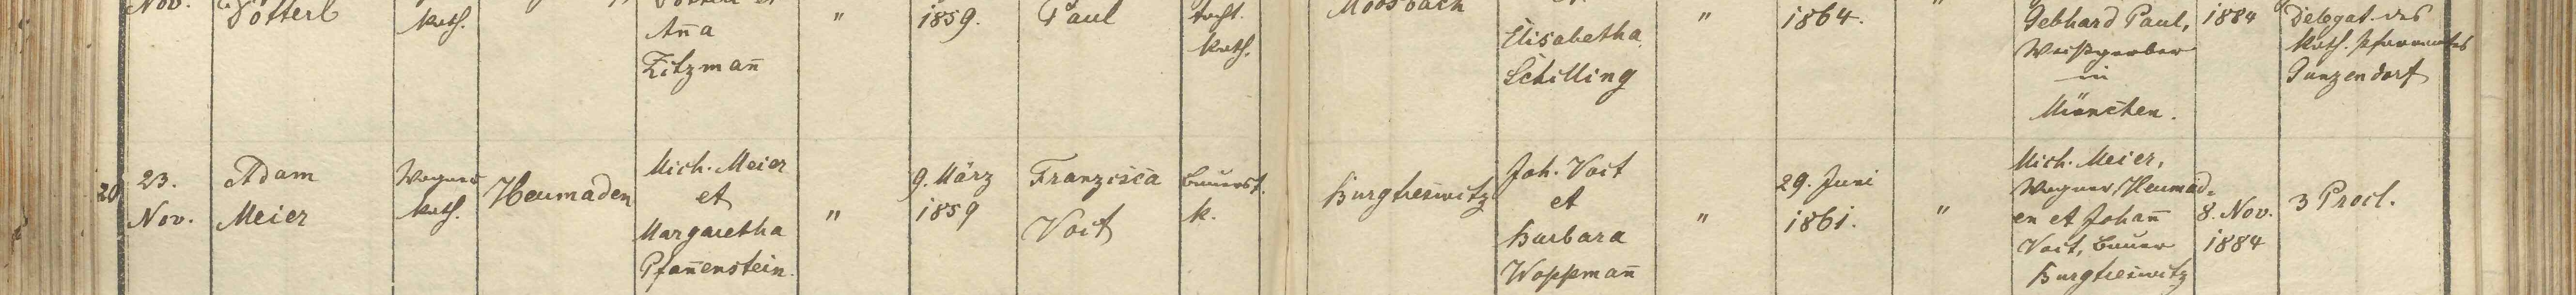
\includegraphics[width=0.85\linewidth,height=\textheight,keepaspectratio,alt={Trauungsbuch Moosbach, Seite 93: Eintrag Nr. 20, die Trauung von Adam Meier, Wagner in Heumaden, mit Franziska Voit, Bauerstochter aus Burgtreswitz, am 23. November 1884, mit den beiden Vätern als Trauzeugen.}]{imagens/doc2_trauung_meier_voit_1884.jpg}
\caption{Trauungsbuch Moosbach, Seite 93: Eintrag Nr. 20, die Trauung
von Adam Meier, Wagner in Heumaden\index[lugares]{heumaden@Heumaden}, mit Franziska Voit\index[pessoas]{voit, franziska@Voit, Franziska}, Bauerstochter
aus Burgtreswitz\index[lugares]{burgtreswitz@Burgtreswitz}, am 23. November 1884, mit den beiden Vätern als
Trauzeugen.}
\end{figure}

Ich machte die Rechnung, die jeder Familienforscher irgendwann macht. Am
23. November 1884, während Adam und Franziska in Moosbach\index[lugares]{moosbach@Moosbach} heirateten,
schlief in Leonberg\index[lugares]{leonberg@Leonberg}, fünfzig Kilometer entfernt, ein vier Monate altes
Kind namens Johann Haas\index[pessoas]{haas, johann@Haas, Johann}. Die Eltern des Fata und die Eltern der Mota\index[pessoas]{meier, maria@Meier, Maria}
kannten sich nicht, haben sich wahrscheinlich nie kennengelernt, und
doch waren in jenem Herbst die beiden Linien schon auf der Karte
gezogen.

Mir fiel auch der Wechsel des Berufs auf. 1884 ist Adam \emph{Wagner},
wie sein Vater. 1888, bei Marias Taufe, ist er \emph{Krämer}, und 1893,
bei Michaels Taufe, \emph{Häusler}, ohne eigenes Ackerland. Der Wagner
behielt weder die Werkstatt, noch bekam er Land. Die Tochter des
Krämers, Maria, sollte für Lohn Kühe melken. Und ihr Enkel wurde Maurer
in Santa Catarina.

\section{Zwei Taufen, eine im Winter und eine im
Sommer}\label{zwei-taufen-eine-im-winter-und-eine-im-sommer}

Es fehlten noch die beiden, die vor dem Altar gestanden hatten. Ich ging
zurück ins Taufbuch, diesmal rückwärts.

Die erste steht auf Seite 96, im Jahr 1859. Die Zeile stammt von einem
Mittwoch im März. Name: \emph{Adam}, dann \emph{Meier}. Hier hat der
Eintrag eine Besonderheit, die ich erst spät verstand. Der Familienname
scheint ausgebessert zu sein, als hätte vorher etwas anderes dort
gestanden, das dann korrigiert wurde. Die Transkription im Dossier, das
diese Dokumente zusammenstellt, deutet das als Legitimation: Adam sei
vor der Heirat seiner Eltern geboren und später anerkannt worden, als
Michael und Margaretha heirateten. Ich bin kein Paläograph, um das mit
Gewissheit zu sagen, darum sage ich nur, was ich sehe: einen Namen, an
dem jemand etwas verändert hat. Wenn die Lesung des Dossiers stimmt,
begann euer Ururgroßvater Georg Adam sein Leben mit einer kleinen
Unregelmäßigkeit, die die Zeit und die Heirat seiner Eltern dann in
Ordnung brachten.

Der Vater: \emph{Michael Meier\index[pessoas]{meier, michael@Meier, Michael}}, \emph{Wagner}, aus Heumaden\index[lugares]{heumaden@Heumaden}. Die
Mutter: \emph{Margaretha Pfannenstein\index[pessoas]{pfannenstein, margaretha@Pfannenstein, Margaretha}}, Bauerstochter. Der mit der
Geburt verbundene Ort: \emph{Rückersrieth\index[lugares]{ruckersrieth@Rückersrieth}}, ihr Dorf. Geburt: \emph{9.
März, 3 Uhr früh}. Taufe: \emph{9. März in Moosbach\index[lugares]{moosbach@Moosbach}}, am selben Tag.
Pfarrer: \emph{idem}. Und der Pate: \emph{Adam Hartung}, Sohn des
Schmieds von Heumaden\index[lugares]{heumaden@Heumaden}.

Da verstand ich, woher der Name kam. In Bayern\index[lugares]{bayern@Bayern} war es üblich, dass das
Kind den Namen des Paten bekam. Georg Adam Meier\index[pessoas]{meier, georg adam@Meier, Georg Adam} hieß Adam wegen Adam
Hartung, dem Schmiedssohn. Der Sohn eines Wagners, getauft auf den Namen
eines Schmiedssohns. Im Dorf arbeiteten Schmied und Wagner zusammen: Der
eine baute das hölzerne Rad, der andere schmiedete den eisernen Reifen,
der es umschloss. Das ganze Rad hing von beiden ab. Ich fand das zu
schön, um bloßer Zufall zu sein, und vielleicht war es das auch nicht.

\begin{ficha}

\textbf{Archivkarte}: Pfarrei St.~Peter und Paul, Moosbach\index[lugares]{moosbach@Moosbach}. Taufbuch
1847--1904 (\texttt{Moosbach\index[lugares]{moosbach@Moosbach}\_Leuchtenberg005}), S. 96. Täufling: Adam
(Georg Adam) Meier. Vater: Michael Meier\index[pessoas]{meier, michael@Meier, Michael}, \emph{Wagner} in Heumaden\index[lugares]{heumaden@Heumaden}.
Mutter: Margaretha Pfannenstein\index[pessoas]{pfannenstein, margaretha@Pfannenstein, Margaretha}, \emph{Bauerstochter}, aus Rückersrieth\index[lugares]{ruckersrieth@Rückersrieth}.
Geburt: 9. März 1859, 3 Uhr morgens. Taufe: 9. März 1859, in Moosbach\index[lugares]{moosbach@Moosbach}.
Pate: Adam Hartung, \emph{Schmiedssohn} aus Heumaden\index[lugares]{heumaden@Heumaden}. Bemerkung: Der
Familienname ist ausgebessert; das paläographische Dossier der Familie
deutet dies als Legitimation durch spätere Heirat der Eltern (vom
Verfasser nicht bestätigte Lesung). Bild:
\texttt{imagens/doc3\_adam\_meier\_1859.jpg}.

\end{ficha}

\begin{figure}
\centering
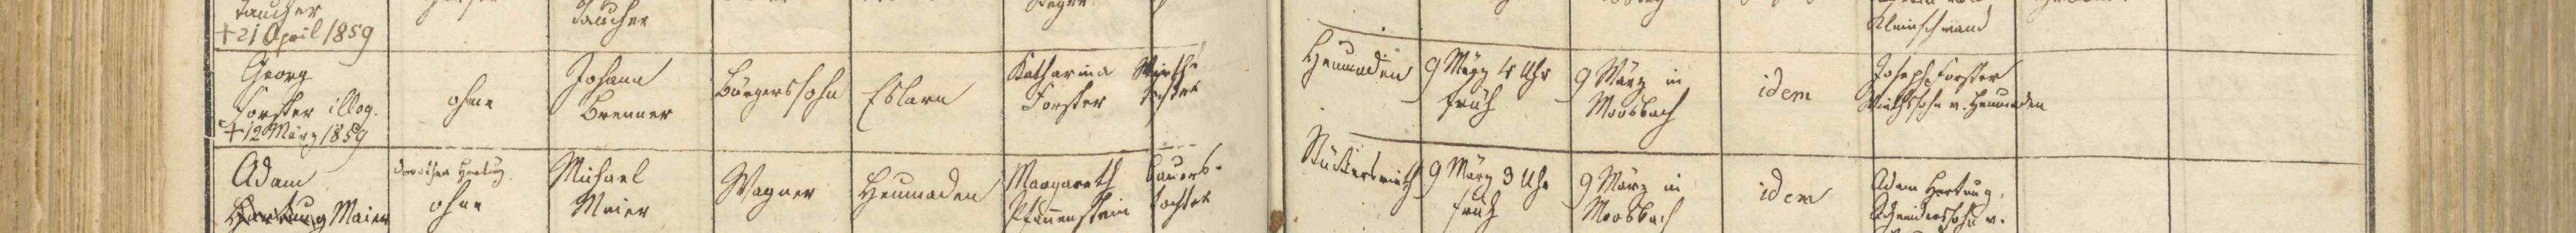
\includegraphics[width=0.85\linewidth,height=\textheight,keepaspectratio,alt={Taufbuch Moosbach, Seite 96: die Taufe von Adam Meier, geboren am 9. März 1859 um drei Uhr nachts, Sohn des Wagners Michael Meier und der Margaretha Pfannenstein, mit Adam Hartung, dem Schmiedssohn aus Heumaden, als Paten.}]{imagens/doc3_adam_meier_1859.jpg}
\caption{Taufbuch Moosbach, Seite 96: die Taufe von Adam Meier, geboren
am 9. März 1859 um drei Uhr nachts, Sohn des Wagners Michael Meier\index[pessoas]{meier, michael@Meier, Michael} und
der Margaretha Pfannenstein\index[pessoas]{pfannenstein, margaretha@Pfannenstein, Margaretha}, mit Adam Hartung, dem Schmiedssohn aus
Heumaden\index[lugares]{heumaden@Heumaden}, als Paten.}
\end{figure}

Die zweite Taufe steht auf Seite 115, zweieinhalb Jahre später, an einem
Samstag im Sommer. Name: \emph{Franziska Voit\index[pessoas]{voit, franziska@Voit, Franziska}}. Vater: \emph{Johann
Voit}, Bauer, aus Treswitz, so hat der Pfarrer Burgtreswitz\index[lugares]{burgtreswitz@Burgtreswitz} abgekürzt.
Mutter: \emph{Barbara Woppmann\index[pessoas]{woppmann, barbara@Woppmann, Barbara}}. Geburt: \emph{29. Juni, Morgens}, also
am Morgen des 29. Juni 1861. Diesmal ohne genaue Stunde. Taufe: am
selben Tag, in Moosbach\index[lugares]{moosbach@Moosbach}. Und der 29. Juni, achtet darauf, ist das Fest
Peter und Paul: Das Mädchen wurde genau am Fest der Pfarrpatrone geboren
und getauft. Ich stelle mir die geschmückte Kirche vor, das feierliche
Hochamt, und mitten im Fest eine Familie aus Burgtreswitz\index[lugares]{burgtreswitz@Burgtreswitz}, die mit einem
wenige Stunden alten Kind ankommt.

Die Hebamme hieß laut Transkription Schmirl. Die Patin: \emph{Margaretha
Albrecht}, Bäuerin.

Albrecht. Ich habe es zweimal gelesen. Jahrelang glaubte ich, Albrecht
sei der Familienname der Mutter von Josef Haas\index[pessoas]{haas, josef@Haas, Josef}, jener Maria Anna
Albrecht aus Stoffen\index[lugares]{stoffen@Stoffen}, und lächelte über den Zufall. Später fand ich
heraus, dass die Maria Anna aus Stoffen\index[lugares]{stoffen@Stoffen} nie zu uns gehört hatte: Sie war
die Mutter eines anderen Joseph Haas. Das Augenzwinkern der Genealogie
war größer, als ich dachte. Die Namen wiederholen sich, und man muss
vorsichtig mit ihnen sein.

\begin{ficha}

\textbf{Archivkarte}: Pfarrei St.~Peter und Paul, Moosbach\index[lugares]{moosbach@Moosbach}. Taufbuch
1847--1904 (\texttt{Moosbach\index[lugares]{moosbach@Moosbach}\_Leuchtenberg005}), S. 115. Täufling:
Franziska Voit\index[pessoas]{voit, franziska@Voit, Franziska}. Vater: Johann Voit\index[pessoas]{voit, johann@Voit, Johann}, \emph{Bauer} in (Burg)Treswitz.
Mutter: Barbara Woppmann\index[pessoas]{woppmann, barbara@Woppmann, Barbara} (\emph{Woppman}). Geburt: 29. Juni 1861,
morgens (\emph{Morgens}). Taufe: 29. Juni 1861, in Moosbach\index[lugares]{moosbach@Moosbach}. Hebamme:
Schmirl (laut Transkription im Dossier). Patin: Margaretha Albrecht,
\emph{Bäuerin}. Bild: \texttt{imagens/doc4\_franziska\_voit\_1861.jpg}.

\end{ficha}

\begin{figure}
\centering
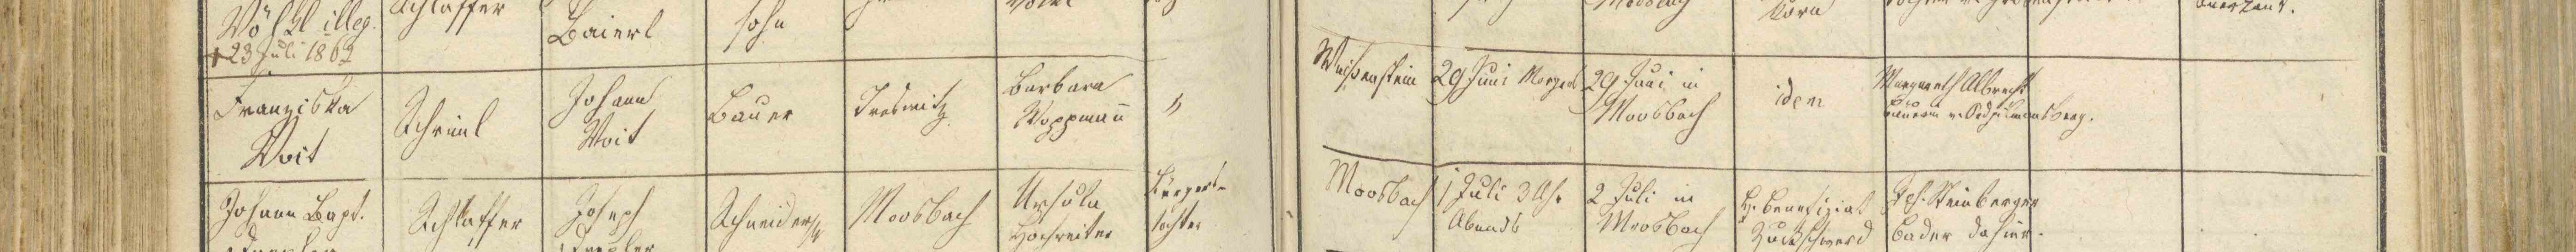
\includegraphics[width=0.85\linewidth,height=\textheight,keepaspectratio,alt={Taufbuch Moosbach, Seite 115: die Taufe von Franziska Voit, geboren am 29. Juni 1861, dem Fest Peter und Paul, Tochter des Bauern Johann Voit aus Burgtreswitz und der Barbara Woppmann.}]{imagens/doc4_franziska_voit_1861.jpg}
\caption{Taufbuch Moosbach, Seite 115: die Taufe von Franziska Voit,
geboren am 29. Juni 1861, dem Fest Peter und Paul, Tochter des Bauern
Johann Voit\index[pessoas]{voit, johann@Voit, Johann} aus Burgtreswitz\index[lugares]{burgtreswitz@Burgtreswitz} und der Barbara Woppmann\index[pessoas]{woppmann, barbara@Woppmann, Barbara}.}
\end{figure}

\section{Das bayerische Puzzle}\label{das-bayerische-puzzle}

Als ich die vier Seiten zu Ende gelesen hatte, war die bayerische Hälfte
eures Stammbaums bis zu den Großeltern der Mota\index[pessoas]{meier, maria@Meier, Maria} vollständig. Ich zeichne
sie euch in Worten, denn so werdet ihr sie im Gedächtnis behalten.

In Heumaden\index[lugares]{heumaden@Heumaden} ein Wagner namens Michael Meier\index[pessoas]{meier, michael@Meier, Michael}. In Rückersrieth\index[lugares]{ruckersrieth@Rückersrieth} eine
Bauerstochter namens Margaretha Pfannenstein\index[pessoas]{pfannenstein, margaretha@Pfannenstein, Margaretha}. Von ihnen wird in einer
Märznacht des Jahres 1859 Georg Adam geboren, der den Namen des
Schmiedssohns erhält.

In Burgtreswitz\index[lugares]{burgtreswitz@Burgtreswitz} ein Bauer namens Johann Voit\index[pessoas]{voit, johann@Voit, Johann} und seine Frau Barbara
Woppmann. Von ihnen wird am Morgen des Patroziniums 1861 Franziska
geboren.

Adam und Franziska heiraten an einem Sonntag im November 1884 in
Moosbach\index[lugares]{moosbach@Moosbach}, mit den beiden Vätern als Trauzeugen. Er baut Räder, später
lebt er vom Land. Sie bekommen Kinder: Maria Katharina 1886, dann, in
einer Aprilnacht 1888, Maria, die Mota\index[pessoas]{meier, maria@Meier, Maria}. Später kommen Theresia\index[pessoas]{meier, theresia@Meier, Theresia} und
Michael. Nach 1893 verschwindet die Familie aus den Moosbacher Büchern
und taucht achtzig Jahre später in Briefen aus Sachsen\index[lugares]{sachsen@Sachsen} wieder auf.

Fünfzig Kilometer entfernt, in Leonberg\index[lugares]{leonberg@Leonberg}, bekommen der Arbeiter Josef
Haas, Sohn von Michael Haas\index[pessoas]{haas, michael@Haas, Michael} und Kunigunde Stadelmann\index[pessoas]{stadelmann, kunigunde@Stadelmann, Kunigunde}, und Franziska
Dengler einen Sohn namens Johann.

Diese beiden Linien werden sich irgendwann vor 1907 treffen. Ich weiß
nicht, wo und wie. Die Hochzeit war in Eibenstock\index[lugares]{eibenstock@Eibenstock}, weit weg von beiden
Dörfern. Vielleicht arbeitete er als Stuckateur auf einer Baustelle in
der Nähe von Heumaden\index[lugares]{heumaden@Heumaden}. Vielleicht ging sie anderswo in Stellung, wie so
viele Mädchen vom Land. Vielleicht lernten sie sich auf einem Fest
kennen, auf einem Markt, an einem Bahnhof. Es gibt kein Dokument. Und
hier endet meine Arbeit als Forscher, und eure beginnt, wenn ihr wollt:
Das Trauungsbuch von Eibenstock\index[lugares]{eibenstock@Eibenstock} existiert, in irgendeinem Archiv in
Sachsen\index[lugares]{sachsen@Sachsen}, und eines Tages wird es jemand aufschlagen.

Am Ende dieses Kapitels denke ich an alles, was die Mota\index[pessoas]{meier, maria@Meier, Maria} nicht erzählt
hat. Sie lebte fünfundachtzig Jahre, sechzig davon in Brasilien, und die
Enkel erinnern sich an eine Großmutter mit blauen Augen und wenigen
Worten Portugiesisch, die viel umarmte. Die Namen Heumaden\index[lugares]{heumaden@Heumaden} und
Burgtreswitz\index[lugares]{burgtreswitz@Burgtreswitz}, der Vater, der Wagner war, der Schmied, dessen Sohn Pate
stand: Nichts davon erreichte uns durch ihre Stimme, oder es kam nur in
Bruchstücken an: das immer wieder gesagte Wort \emph{Heumaden\index[lugares]{heumaden@Heumaden}}, ein
Tonfall, eine Erinnerung an Kühe. Der Rest blieb in der Schrift
verwahrt, die sie lesen konnte und wir nicht. Es brauchte einen Enkel,
der die Kurrentschrift lernte, damit sie uns endlich erzählte, woher sie
kam.

Ein letzter Punkt auf der Karte fehlte noch. Zehn Tage nach
Maxhütte-Haidhof\index[lugares]{maxhutte-haidhof@Maxhütte-Haidhof} sollte ich in London auf einer Metalllinie stehen, an
dem Ort, an dem die Menschheit vereinbart hat, dass alle Längengrade
beginnen.

\section{Für euch zum Entdecken}\label{fuxfcr-euch-zum-entdecken-17}

\begin{itemize}
\tightlist
\item
  War Katharina Reichenberger, die Patin aus Burgtreswitz\index[lugares]{burgtreswitz@Burgtreswitz}, die Tante
  Katharina der Überlieferung, eine geborene Meier, die einen
  Reichenberger geheiratet hatte? Sucht den Trauungseintrag in
  Burgtreswitz\index[lugares]{burgtreswitz@Burgtreswitz}, den ich noch nicht gelesen habe.
\item
  Was stand vor der Ausbesserung im Familiennamen von Adam auf Seite 96?
  Das Bild liegt unter \texttt{imagens/doc3\_adam\_meier\_1859.jpg}. War
  es wirklich eine Legitimation?
\item
  Wo haben sich ein Stuckateur aus Leonberg\index[lugares]{leonberg@Leonberg} und ein Mädchen aus Heumaden\index[lugares]{heumaden@Heumaden}
  kennengelernt, und warum haben sie in Eibenstock\index[lugares]{eibenstock@Eibenstock} geheiratet? Das
  dortige Trauungsbuch liegt in irgendeinem Archiv in Sachsen\index[lugares]{sachsen@Sachsen} und wartet
  darauf, dass jemand es aufschlägt.
\item
  Was hat die Mota\index[pessoas]{meier, maria@Meier, Maria}, außer dem Wort \emph{Heumaden\index[lugares]{heumaden@Heumaden}} und der Erinnerung an
  die Kühe, den Enkeln von ihrer Heimat erzählt? Fragt die Vettern und
  Basen, die sie gekannt haben.
\end{itemize}

\chapter{Mit beiden Füßen auf dem Nullmeridian}\label{cap-19}

\emph{51,48° N · 0,00°, Königliche Sternwarte, Greenwich, London}

\begin{quote}
\emph{Jede Messung beginnt an einem gewählten Ort. Worauf es ankommt,
ist, von dort aus ehrlich zu messen.}
\end{quote}

Die Linie, die die Touristen in Greenwich fotografieren, ist nicht der
Längengrad null, den ihr Handy benutzt.

\section{Eine Linie aus Messing}\label{eine-linie-aus-messing}

Am Freitag, dem 16. Februar 2018, zehn Tage nach Maxhütte-Haidhof\index[lugares]{maxhutte-haidhof@Maxhütte-Haidhof}, war
ich in Greenwich, oben auf dem Hügel der Königlichen Sternwarte über der
Themse, östlich der Londoner Innenstadt. Dort gibt es eine Linie. Es ist
ein Metallstreifen, der in den Boden des Hofes eingelassen ist, quer
über die Steine läuft und den Meridian von Greenwich markiert, den
Längengrad null. Auf der einen Seite die östliche Halbkugel, auf der
anderen die westliche. Die Touristen stehen Schlange, um einen Fuß auf
jede Seite zu setzen und ein Foto zu machen. Ein Physiklehrer, der sein
Leben lang Koordinaten unterrichtet hat, ist gegen diese Versuchung
nicht gefeit; keine akademische Würde hält einer solchen Linie stand,
und die Überschrift dieses Kapitels verrät, auf welcher Seite der
Schlange ich stand.

Hinter der Linie steckt eine Geschichte, die ich schon vor der Reise
kannte und die nach jenem Winter für mich eine andere Bedeutung bekam.
Bis ins 19. Jahrhundert zählte jedes Land die Längengrade von seinem
eigenen Meridian aus: die Franzosen von Paris, die Spanier von Cádiz,
die Portugiesen von Lissabon oder anderen Punkten, und so weiter. Karten
verschiedener Nationen passten nicht zusammen. Schiffe tauschten
Positionen aus, die nicht übereinstimmten. Es brauchte eine
internationale Konferenz in Washington, damit sich gut zwanzig Länder
darauf einigten, einen einzigen Nullmeridian für die ganze Welt zu
verwenden. Sie wählten Greenwich. Die Konferenz tagte im Oktober 1884.

Oktober 1884. Drei Monate nachdem Josef Haas\index[pessoas]{haas, josef@Haas, Josef} in Leonberg\index[lugares]{leonberg@Leonberg} den Eintrag Nr.
47 unterschrieben hatte. Einen Monat bevor Adam Meier und Franziska Voit\index[pessoas]{voit, franziska@Voit, Franziska}
in Moosbach\index[lugares]{moosbach@Moosbach} heirateten. In demselben Herbst, in dem eure beiden
bayerischen Linien gezogen wurden, vereinbarte die Menschheit, von wo
aus man von nun an die Lage aller Dinge zählen würde. Natürlich gibt es
zwischen diesen Ereignissen keinen ursächlichen Zusammenhang. Aber ein
Meteorologe lebt von zeitlichen Zufällen: Indem man betrachtet, was zur
gleichen Zeit an verschiedenen Orten geschieht, entdeckt man die
Struktur eines Systems. Und ich denke gern daran, dass der Fata\index[pessoas]{haas, johann@Haas, Johann} in dem
Jahr geboren wurde, in dem die Welt einen Nullmeridian bekam.

Zurück zum Handy, dem technischen Detail, das die Physiker freut, die
Greenwich besuchen. Die Metalllinie markiert den historischen Meridian,
festgelegt durch die Achse eines Teleskops, das dort im 19. Jahrhundert
aufgestellt wurde. Das Bezugssystem aber, das heute die
Navigationssatelliten verwenden und mit dem das GPS unserer Handys
arbeitet, legt den Längengrad null etwa hundert Meter östlich der
Metalllinie. Der Unterschied kommt daher, wie jedes System die
Senkrechte und die Form der Erde festlegt. Wer mit einem Fuß auf jeder
Seite des Streifens steht und aufs Handy schaut, stellt fest, dass er
sich für den Satelliten vollständig auf der westlichen Halbkugel
befindet.

Ich fand darin eine Lektion über Genealogie. Der Ursprung, den die
Familie fotografiert, und der Ursprung, den die Dokumente verzeichnen,
decken sich selten genau. Der Fata\index[pessoas]{haas, johann@Haas, Johann} hatte laut Tabelle am 8. Juli
Geburtstag; das Standesamt sagt den 11. Die Mota\index[pessoas]{meier, maria@Meier, Maria} war auf der
Passagierliste 25 Jahre alt und in Wirklichkeit 24. Ihre Patin war in
der Erinnerung die Tante Katharina Meier und im Buch Katharina
Reichenberger. Beide Ursprünge gibt es, und der Abstand zwischen ihnen
beträgt ein paar Meter, ein paar Tage, einen Ehenamen. Die Arbeit des
Forschers ist es, diesen Abstand zu messen und ihn auszusprechen.

\section{Jede Familie wählt ihren
Meridian}\label{jede-familie-wuxe4hlt-ihren-meridian}

Der Längengrad null ist nicht natürlich. Das sage ich meinen Studenten
immer, und sie brauchen lange, um es zu akzeptieren. Die Breite hat
einen physikalischen Ursprung: Der Äquator ist der Kreis, auf dem die
Rotationsachse der Erde senkrecht zur Oberfläche steht, und jede
Zivilisation auf jedem Planeten würde zu ihm gelangen. Aber es gibt
keinen physikalischen Grund, warum der Längengrad null durch Greenwich
gehen sollte und nicht durch Paris, Rom oder Florianópolis\index[lugares]{florianopolis@Florianópolis}. Es ist eine
Übereinkunft. Und doch funktioniert ohne diese Wahl keine Karte. Wir
brauchen einen Punkt, von dem aus wir zählen.

Jede Familie macht es genauso. Sie wählt einen Punkt und zählt von ihm
aus. Für die mehr als sechshundert Nachkommen, die sich im März 2013
versammelten, war der Nullmeridian die Ankunft von Johann und Maria in
Brasilien 1913: Von dort aus wurde das Jubiläum gezählt. Für Agenors
Tabelle war das Ehepaar der Nullmeridian, und alles wurde in Kindern,
Enkeln, Urenkeln und Ururenkeln gezählt. Für dieses Buch seid ihr beide
der Nullmeridian. Der Stammbaum, den ich angelegt habe, sagt das ganz
deutlich: Matheus und Lucas sind die Generation G1, und alles andere
wird von euch aus rückwärts gezählt: G2 für die Eltern, G3 für die
Großeltern, bis G8, die Urururururgroßeltern aus Harderode\index[lugares]{harderode@Harderode} und aus
Schleswig-Holstein.

Ich habe es so gewählt, weil es der einzige Weg ist, Menschen, die sich
nie begegnet sind, in einem einzigen Stammbaum unterzubringen. Die Haas
aus Bayern\index[lugares]{bayern@Bayern} und die Lohmann aus Niedersachsen wussten nie voneinander.
Die Michels aus Hermeskeil\index[lugares]{hermeskeil@Hermeskeil} und die Funke aus Joinville\index[lugares]{joinville@Joinville} lebten in
verschiedenen Jahrhunderten. Der Punkt, an dem sich all diese Linien
kreuzen, ist ein Haus in Florianópolis\index[lugares]{florianopolis@Florianópolis}, in dem zwei Jungen wohnen (heute
zwei Männer). Ihr seid der Schnittpunkt. Darum seid ihr der Ursprung.

Ich will dazu etwas sagen, da ich nun schon auf einem willkürlichen
Ursprung stehe. Der Nullmeridian einer Familie zu sein ist eine
Verantwortung. Von euch aus wird eines Tages jemand die Generationen neu
zählen. In hundert Jahren werden die Kinder eurer Kinder ihren eigenen
Meridian wählen, und ihr werdet G2, G3, G4 sein. Ihr werdet in der Mitte
des Stammbaums stehen, nicht an seiner Spitze. Das geschieht mit jedem.
Es geschah mit dem Fata\index[pessoas]{haas, johann@Haas, Johann} und der Mota\index[pessoas]{meier, maria@Meier, Maria}, die einmal der Mittelpunkt von
allem waren und heute G4 sind.

Es gibt ein Bild aus meinem Beruf, das dies besser zusammenfasst, als
ich es kann. Es heißt allgemeine Zirkulation der Atmosphäre. Wenn ihr
den ganzen Planeten aus der Ferne betrachtet, wirkt der Wind chaotisch:
hier Stürme, dort Flauten, Fronten, Zyklone, Brisen. Aber im Mittel
vieler Jahre ordnet er sich in großen Zellen, die um die ganze Welt
laufen. In Äquatornähe steigt warme Luft auf, strömt in der Höhe zu den
Polen, sinkt um den dreißigsten Breitengrad herum ab und kehrt in
Bodennähe als Passatwind zurück: Das ist die Hadley-Zelle, die die
Segelschiffe von 1828 und 1847 vorantrieb und sie in den Kalmen
festhielt. In höheren Breiten andere Zellen, andere Winde: die
Westwinde, die über Europa und den Süden Brasiliens fegen, die
Polarluft, die in Wellen herabsteigt. Keine dieser Zellen existiert für
sich allein. Jede hängt von ihren Nachbarn ab. Die Luft, die in Belém
aufsteigt, sinkt eines Tages über der Sahara oder dem Südatlantik ab;
die Kälte, die in der Antarktis entsteht, kommt eines Tages als Frost in
Vidal Ramos\index[lugares]{vidal ramos@Vidal Ramos} an. Es ist ein einziges System.

Eine Familie ist genauso. Aus der Nähe ist sie ein Durcheinander von
Menschen, die geboren werden, heiraten, streiten, auswandern, sterben,
den Kontakt verlieren, Namen und Sprache wechseln. Aus der Ferne, über
zweihundert Jahre betrachtet, ist sie eine Zirkulation. Menschen, die
von der Mosel\index[lugares]{mosel@Mosel} aufbrechen und in Desterro\index[lugares]{desterro@Desterro} ankommen. Menschen, die die
Oberpfalz\index[lugares]{oberpfalz@Oberpfalz} verlassen und in Rio de Janeiro\index[lugares]{rio de janeiro@Rio de Janeiro} ankommen. Menschen, die von
der Küste ins Alto Vale ziehen, vom Alto Vale nach Paraná, von Rio
Grande nach Joinville\index[lugares]{joinville@Joinville}, von Joinville und Vidal Ramos\index[lugares]{vidal ramos@Vidal Ramos} nach Florianópolis\index[lugares]{florianopolis@Florianópolis}.
Ab und zu geht jemand den Weg zurück, so wie ich in jenem Winter, und
schließt die Zelle.

\section{Die Koordinaten der Familie}\label{die-koordinaten-der-familie}

Der Stammbaum, den ich aus FamilySearch exportiert habe, enthält
achtundfünfzig geographische Koordinaten. Es sind die Orte, an denen die
Familie geboren wurde, geheiratet hat, gestorben und angekommen ist. Ich
stelle mir vor, wie ich sie, gerundet, auf dem Längengrad null stehend
aufsage, so wie man einen Rosenkranz betet. Ich tue das hier für euch,
langsam, von Osten nach Westen, denn das ist die Richtung, in die die
Familie gegangen ist.

Der östlichste Punkt von allen ist Bayern\index[lugares]{bayern@Bayern}. Leonberg\index[lugares]{leonberg@Leonberg}, heute
Maxhütte-Haidhof\index[lugares]{maxhutte-haidhof@Maxhütte-Haidhof}, auf 49,2 Nord und 12,1 Ost. Heumaden\index[lugares]{heumaden@Heumaden}, Rückersrieth\index[lugares]{ruckersrieth@Rückersrieth} und
Burgtreswitz\index[lugares]{burgtreswitz@Burgtreswitz} rund um Moosbach\index[lugares]{moosbach@Moosbach}, auf 49,6 Nord und 12,4 Ost. Das sind die
Haas, die Meier, die Voit.

Ein Stück weiter westlich und nördlich Niedersachsen: Harderode\index[lugares]{harderode@Harderode}, die
Heimat der Lohmann, bei Hameln\index[lugares]{hameln@Hameln}, auf 52 Nord und 9,4 Ost, und noch weiter
nördlich Schleswig-Holstein, woher die Schnack kamen. Das ist die
Familie eurer Mutter.

Dann, nach Südwesten hinab, das Rheinland und die Mosel\index[lugares]{mosel@Mosel}, die Heimat
derer, die zuerst kamen. Solingen\index[lugares]{solingen@Solingen}, die Klingenstadt, aus der die
Überlieferung die Doerner und die Lauterjung kommen lässt, auf 51,2 Nord
und 7,1 Ost, fast genau auf der Breite von Greenwich, wo ich stand.
Pünderich\index[lugares]{punderich@Pünderich} in der Moselschleife, die Heimat von Angela Catharina Arns\index[pessoas]{arns, angela catharina@Arns, Angela Catharina},
auf 50 Nord und 7,1 Ost. Hermeskeil\index[lugares]{hermeskeil@Hermeskeil}, wo der kleine Anton Michels\index[pessoas]{michels, anton@Michels, Anton} geboren
wurde, und Schweich\index[lugares]{schweich@Schweich}, der Ort von Bernard Preis\index[pessoas]{preis, bernard@Preis, Bernard}, beide bei Trier, auf
etwa 49,7 Nord und weniger als 7 Grad Ost.

Dann die Nulllinie. Greenwich. Der einzige Ort auf dieser Liste, der
nichts mit der Familie zu tun hat, außer dass ich dort gewesen bin.

Dann der Ozean. Auf der anderen Seite, mit umgekehrtem Vorzeichen bei
Breite und Länge, als ginge man durch einen Spiegel: Rio de Janeiro\index[lugares]{rio de janeiro@Rio de Janeiro}, wo
die \emph{Formosa} die Familie am 26. März 1913 an Land setzte, auf 22,9
Süd und 43,2 West; und Laguna\index[lugares]{laguna@Laguna}, das Tor nach Santa Catarina, auf das die
Überlieferung zeigt, auf 28,5 Süd und 48,8 West. São Pedro de Alcântara\index[lugares]{sao pedro de alcantara@São Pedro de Alcântara},
die erste deutsche Kolonie in Santa Catarina, auf 27,6 Süd und 48,8
West. Anitápolis\index[lugares]{anitapolis@Anitápolis} und der Rio do Ouro\index[lugares]{rio do ouro@Rio do Ouro}, das Lote 17, auf 27,9 Süd und 49,1
West. São Martinho\index[lugares]{sao martinho@São Martinho} und Vargem do Cedro\index[lugares]{vargem do cedro@Vargem do Cedro}, die Heimat der Preiss und der
Michels, auf etwas mehr als 28 Süd. Brusque\index[lugares]{brusque@Brusque}, wo Fernando Dörner\index[pessoas]{dorner, fernando@Dörner, Fernando} und
Gertrudes Preiss\index[pessoas]{preiss, gertrudes@Preiss, Gertrudes} liegen, auf 27,1 Süd. Ituporanga\index[lugares]{ituporanga@Ituporanga}, Rio Novo\index[lugares]{rio novo@Rio Novo}, Águas
Negras, auf 27,4 Süd und 49,6 West. Vidal Ramos\index[lugares]{vidal ramos@Vidal Ramos}, das Haus meiner Eltern,
auf 27,4 Süd und 49,4 West. Aurora\index[lugares]{aurora@Aurora} und Ribeirão das Pacas\index[lugares]{ribeirao das pacas@Ribeirão das Pacas}, wo der Fata\index[pessoas]{haas, johann@Haas, Johann}
und die Mota\index[pessoas]{meier, maria@Meier, Maria} liegen, umgeben von den Gräbern, die er gemacht hat, auf
27,3 Süd und 49,6 West. Weiter südlich und westlich, in Rio Grande,
Estrela\index[lugares]{estrela@Estrela} und Arroio do Meio\index[lugares]{arroio do meio@Arroio do Meio}, das Haus der Lohmann in Palmas\index[lugares]{palmas@Palmas} am Ufer des
Taquari, auf 29,3 Süd und 51,9 West. Joinville\index[lugares]{joinville@Joinville}, die Heimat der Funke und
der Oma Rosita\index[pessoas]{lohmann, rosita erica@Lohmann, Rosita Érica}, auf 26,3 Süd und 48,8 West. Und schließlich
Florianópolis\index[lugares]{florianopolis@Florianópolis}, auf 27,6 Süd und 48,5 West. Euer Zuhause.

Achtet auf etwas, das nur ein Meteorologe der Rede wert fände: Die
beiden Hälften der Familie leben in vertauschten Jahreszeiten. Wenn in
Heumaden\index[lugares]{heumaden@Heumaden} Winter ist, ist in Aurora\index[lugares]{aurora@Aurora} Sommer. Die Mota\index[pessoas]{meier, maria@Meier, Maria} wurde in einem
bayerischen Frühling geboren, im April, und kam am Ende eines Sommers
nach Brasilien, im März, und im ersten Jahr in Santa Catarina muss sie
sich über Weihnachten in der Hitze gewundert haben und über den
Johannistag, in Bayern\index[lugares]{bayern@Bayern} ein Sommerfest, in der Kälte. Für ihre Urenkel,
also euch, ist der Juli ein Monat für Jacken und der Dezember ein Monat
für den Strand; in Heumaden\index[lugares]{heumaden@Heumaden} fiele jeder eurer Geburtstage in die
entgegengesetzte Jahreszeit. Der Fata\index[pessoas]{haas, johann@Haas, Johann}, im Juli geboren, in einem
bayerischen Sommer, verbrachte mehr als fünfzig Geburtstage in
Brasilien, alle im Winter. Ich werde nie erfahren, ob ihm an seinem
Geburtstag der Sommer fehlte. Ich nehme es an.

Wenn ihr all diese Punkte auf einer Karte einzeichnet, seht ihr zwei
Wolken: eine in der Mitte Europas, zwischen 48 und 54 Grad Nord, und
eine im Süden Brasiliens, zwischen 26 und 30 Grad Süd. Dazwischen der
ganze Atlantik, durchzogen von Pfeilen: 1828, 1846, 1847, 1913. Alle
Pfeile enden, auf die eine oder andere Weise, am selben Punkt. Ein
Vorschlag, den ich dem Verlag hinterlasse, falls dieses Buch einen
bekommt: Diese Karte sollte auf das Vorsatzblatt, als Erstes, was man
beim Aufschlagen sieht.

\section{Drei Flüsse, ein einziger
Regen}\label{drei-fluxfcsse-ein-einziger-regen}

Etwas zeigt die brasilianische Punktwolke, was die europäische nicht
zeigt: Fast alle Punkte liegen an einem Fluss. Davon habe ich in Teil V
erzählt, und ich greife hier nur das Wesentliche auf, denn in Greenwich,
vor der Themse, dachte ich an unsere Flüsse.

Der Tubarão\index[lugares]{tubarao@Tubarão}, der aus dem Gebirge herabkommt und in die Lagune mündet,
und der im März 1974 nach den meistgenannten Zahlen etwa zweihundert
Menschen tötete und die Stadt ertränkte, einundsechzig Jahre nach dem
Jahr, in dem die Haas der Überlieferung nach durch Laguna\index[lugares]{laguna@Laguna} kamen, an der
Mündung eben dieses Flusses. Der Itajaí\index[lugares]{itajai@Itajaí} mit seinen Armen, der Itajaí do
Sul, der an Ituporanga\index[lugares]{ituporanga@Ituporanga} vorbeifließt, wo nach den großen Hochwassern die
Barragem Sul gebaut wurde, und der Itajaí\index[lugares]{itajai@Itajaí}-Mirim, der an Brusque\index[lugares]{brusque@Brusque}
vorbeifließt, wo die Eltern von Oma Adelina liegen; der Fluss der
Hochwasser von 1880, 1911, 1983, 1984, 2008 und 2011. Und der Taquari in
Rio Grande, an dem das Haus der Lohmann steht und der im Mai 1941, im
September und November 2023 und im Mai 2024 höher stieg als alles, was
die Familie je gesehen hatte.

Die Einwanderer ließen sich an den Flüssen nieder, weil das Wasser
Straße war, Kraft für die Mühle, flaches und fruchtbares Land in den
Auen. Und weil sie es nicht wussten. Niemand hatte ihnen gesagt, dass
diese Flüsse in wenigen Tagen um mehr als zehn Meter steigen konnten.
Die drei Flüsse der Familie werden von derselben atmosphärischen
Maschine gespeist: der Feuchtigkeit aus dem Amazonasgebiet, die von
einer tief liegenden Windströmung östlich der Anden nach Süden getragen
wird; den Fronten, die über dem Süden Brasiliens liegen bleiben; den
Zyklonen, die sich an der Küste bilden; und in El-Niño-Jahren dem Regen,
der nicht aufhört. Drei Flüsse, ein einziger Regen. Diesen Regen zu
erforschen ist meine Arbeit. Ich habe diese Arbeit nicht wegen der
Familie gewählt. Aber seit ich dieses Buch geschrieben habe, kann ich
das eine nicht mehr vom anderen trennen.

Dann war da noch das Erbe, das Thema von Kapitel 15. In Europa das Land,
das an der Mosel\index[lugares]{mosel@Mosel} und im Hunsrück\index[lugares]{hunsruck@Hunsrück} geteilt wurde, bis nichts mehr übrig
war, und das die Michels, die Arns und die Preis ans Meer trieb; und das
Land, das im alten Bayern\index[lugares]{bayern@Bayern} ungeteilt an einen einzigen Sohn ging und die
anderen in die Werkstätten und Hütten trieb, wie den Arbeiter Josef. In
Brasilien die Kolonielose und die Familien mit zehn, zwölf, fünfzehn
Kindern (der Fata\index[pessoas]{haas, johann@Haas, Johann} hatte elf, der Ururgroßvater Carlos Doerner fünfzehn,
Francisco Lohmann\index[pessoas]{lohmann, francisco jacob@Lohmann, Francisco Jacob} zwölf) und wieder die Notwendigkeit fortzugehen: ins
Alto Vale, in den Westen, nach Paraná. In fast allen Zweigen gibt es
Menschen, die das Land nicht bekamen und deshalb weiterzogen. Ihr seid
das Ergebnis vieler, die nichts erbten.

\section{Die Anden, kurz}\label{die-anden-kurz}

Ich will von den Anden sprechen, weil sie einen Kreis schließen, aber
ich fasse mich kurz, wie ich es mir vorgenommen habe, als ich dieses
Buch plante.

Auf einer anderen Reise, mit eurer Mutter und mit euch beiden, haben wir
die Kordilleren überquert und waren in Valparaíso, in Santiago, in Valle
Nevado. Diese Reise erzähle ich hier nicht. Sie gehört euch, und ihr
werdet sie erzählen, wie ihr wollt, wenn ihr wollt. Ich will nur
festhalten, was sie in der Geometrie dieses Buches bedeutete.

Die Anden sind für das Klima im Süden Brasiliens das, was die Alpen für
Europa sind: eine Wand. Ihretwegen entweicht die Feuchtigkeit aus dem
Amazonasgebiet nicht zum Pazifik, sondern wird nach Süden umgelenkt und
kommt als Regen in den Tälern des Itajaí\index[lugares]{itajai@Itajaí} und des Taquari an. Ohne die
Anden wären die drei Flüsse der Familie andere. Jedes Hochwasser, von
dem ich in Teil V erzählt habe, hat einen Teil seines Ursprungs an einem
Andenhang.

Dort, an dieser Wand, sah ich euch eure eigene Überquerung machen, die
von Menschen, die nicht mehr fortgehen müssen, um zu überleben, und
darum gehen können, um kennenzulernen. Johann und Maria überquerten die
Alpen, um nie wieder zurückzukehren. Ich überquerte die Alpen, um ein
Papier zu holen, und kehrte zurück. Ihr habt die Anden überquert und
seid ebenfalls zurückgekehrt, und ihr werdet andere Berge überqueren,
und ich weiß nicht, welche. Der Kompass ging zu diesem Zeitpunkt schon
in andere Hände über.

\section{Die Rückkehr}\label{die-ruxfcckkehr}

Von Greenwich bewahre ich sicher das Datum und die Linie. Der Rest ist
das, was der Februar in London gewöhnlich mit den Füßen eines
Catarinense anstellt, und der Kopf voller Zahlen, den ein solcher Ort
jedem Physiker hinterlässt.

In der Mappe trug ich die Abschrift des Eintrags Nr. 47 aus Leonberg\index[lugares]{leonberg@Leonberg}.
Ich trug die Angaben zu den vier Einträgen aus Moosbach\index[lugares]{moosbach@Moosbach}. Ich trug die
Auskunft, dass ein Haas, 1941 in Leonberg\index[lugares]{leonberg@Leonberg} geboren, in den Unterlagen der
Stadt verzeichnet war. Vor allem trug ich das seltene Gefühl, das
Meteorologen kaum kennen, dass sich eine Vorhersage bestätigt hatte. Die
Frage, die dieses Buch antrieb, \emph{gibt es auf der anderen Seite noch
jemanden?}, hatte eine Antwort. Ja. Es gibt Bücher mit ihren Namen, und
es gibt mindestens einen Menschen mit ihrem Familiennamen, in derselben
Stadt.

Nun musste ich das nach Hause bringen. In das Haus in Florianópolis\index[lugares]{florianopolis@Florianópolis}, wo
ihr seid. Und in das Haus in Vidal Ramos\index[lugares]{vidal ramos@Vidal Ramos}, wo der letzte lebende Mensch
jener Generation war, die den Fata\index[pessoas]{haas, johann@Haas, Johann} und die Mota\index[pessoas]{meier, maria@Meier, Maria} aus der Nähe gekannt
hatte: meine Mutter, Oma Adelina, ihre Schwiegertochter, die 1947 in die
Familie kam und mehr als zwei Jahrzehnte mit ihnen lebte.

Sie war in jenem Februar 91 Jahre alt. Sie sollte noch ein Jahr leben.

Die Heimreise, auf welchem Weg auch immer, würde ohne Feierlichkeit
wieder alle Linien überqueren, deren Zeichnen ich mein Leben lang
gelehrt hatte. Den Äquator, wo das Vorzeichen der Breite umschlägt. Den
Wendekreis. Der Längengrad null bliebe zurück, dann 10 Grad West, 20,
30, 40. Bei 48,5 wären wir zu Hause.

\section{Für euch zum Entdecken}\label{fuxfcr-euch-zum-entdecken-18}

\begin{itemize}
\tightlist
\item
  Ist der 1941 in Leonberg\index[lugares]{leonberg@Leonberg} geborene Haas, von dem ich in der Mappe
  Nachricht trug, mit euch verwandt? Das entscheidet nur ein Dokument.
\item
  Woher kam der 8. Juli, den Agenor\index[pessoas]{haas, agenor@Haas, Agenor} in die Tabelle eintrug, wenn das
  Standesamt den 11. nennt? Fragt die Vettern und Basen, an welchem Tag
  die Familie den Geburtstag des Fata\index[pessoas]{haas, johann@Haas, Johann} feierte.
\item
  Wie viele der achtundfünfzig Koordinaten im Stammbaum liegen weit weg
  von einem Fluss? Zeichnet die Karte und zählt.
\item
  Wer unter den Nachkommen des Fata\index[pessoas]{haas, johann@Haas, Johann} und der Mota\index[pessoas]{meier, maria@Meier, Maria} ist noch den Weg zurück
  nach Europa gegangen? Fragt die Lebenden.
\end{itemize}

\chapter*{Epilog --- Der Kompass für Matheus und Lucas}\markboth{Epilog --- Der Kompass für Matheus und Lucas}{Epilog --- Der Kompass für Matheus und Lucas}\label{epilogo}
\addcontentsline{toc}{chapter}{Epilog --- Der Kompass für Matheus und
Lucas}

\emph{27,4° S · 49,4° W, Vidal Ramos\index[lugares]{vidal ramos@Vidal Ramos} · 27,6° S · 48,5° W, Florianópolis\index[lugares]{florianopolis@Florianópolis}}

\begin{quote}
\emph{Der Stammbaum wird nie fertig. Er wechselt nur die Hände.}
\end{quote}

\section{Der 22. Februar 2019}\label{der-22.-februar-2019}

Oma Adelina starb am 22. Februar 2019 in Vidal Ramos\index[lugares]{vidal ramos@Vidal Ramos}. Sie war 92 Jahre
alt. Etwas mehr als ein Jahr zuvor hatte ich in Maxhütte-Haidhof\index[lugares]{maxhutte-haidhof@Maxhütte-Haidhof} vor dem
Buch von 1884 gestanden, und etwas mehr als fünf Jahre zuvor, im
Dezember 2013, war Opa Baldoíno gegangen.

Über diesen Tag werde ich nicht viel schreiben. Es gibt Dinge, die ein
Sohn für sich behält, und dieses Buch hat von Anfang an versprochen, nur
zu erzählen, was es belegen kann. Den Tod einer Mutter belegt man nicht.
Man nennt das Datum, und wer bis hierher gelesen hat, weiß den Rest.

Ich will sagen, wer sie für diese Geschichte war, denn ohne sie gäbe es
kein Buch. Adelina Doerner\index[pessoas]{doerner, adelina@Doerner, Adelina} wurde am 30. Oktober 1926 in São Martinho\index[lugares]{sao martinho@São Martinho}
geboren, als Tochter von Fernando Dörner\index[pessoas]{dorner, fernando@Dörner, Fernando} und Gertrudes Preiss\index[pessoas]{preiss, gertrudes@Preiss, Gertrudes}.
Väterlicherseits stammte sie von den Dörner aus dem Rheinland ab, die
die Überlieferung mit den Messerschmieden von Solingen\index[lugares]{solingen@Solingen} verbindet, und
von den Eller aus Westfalen\index[lugares]{westfalen@Westfalen}. Mütterlicherseits von den Preis aus
Schweich\index[lugares]{schweich@Schweich}, den Michels aus Hermeskeil\index[lugares]{hermeskeil@Hermeskeil} und der langlebigen Angela
Catharina Arns aus Pünderich\index[lugares]{punderich@Pünderich}. Sie heiratete 1947 Baldoíno Haas\index[pessoas]{haas, baldoino@Haas, Baldoíno} und
vereinte, ohne es zu wissen, die beiden großen Strömungen dieses Buches:
die von 1828 und 1847, die mit dem Segelschiff kam und die ersten
Lichtungen bei Desterro\index[lugares]{desterro@Desterro} schlug, und die von 1913, die mit dem Dampfer
kam und ins Alto Vale hinaufzog. Im Mai 2012, bei der Eisernen Hochzeit
nach 65 Ehejahren, ließ sie sich vor einer Kamera aufnehmen und nannte
Namen von Onkeln, von Orten, von Flüssen. Dieses Video war das erste
Dokument dieser Forschung. Ihre Stimme eröffnet das Buch, in Kapitel 1,
und es ist nur recht, dass ihr Fehlen es beschließt.

Sie kannte den Fata\index[pessoas]{haas, johann@Haas, Johann} und die Mota\index[pessoas]{meier, maria@Meier, Maria}. Sie war ihre Schwiegertochter und
lebte mehr als zwei Jahrzehnte mit den beiden. Als der Fata\index[pessoas]{haas, johann@Haas, Johann} 1969 starb,
war ich noch keine vier Jahre alt. Als die Mota\index[pessoas]{meier, maria@Meier, Maria} 1973 starb, war ich
acht. Meine Erinnerungen an sie sind zerfasert, fast Schatten. Ihre
waren vollständig. Jahrelang war sie in unserem Haus die letzte lebende
Zeugin dafür, wie die beiden sprachen, gingen, lachten.

Ich würde hier gern schreiben, dass ich mich nach meiner Rückkehr aus
Bayern\index[lugares]{bayern@Bayern} in der Küche in Vidal Ramos\index[lugares]{vidal ramos@Vidal Ramos} neben sie setzte und ihr die
Abschrift des Eintrags Nr. 47 in die Hände legte, die Unterschrift von
Josef Haas\index[pessoas]{haas, josef@Haas, Josef}, die Seite 441 aus Moosbach\index[lugares]{moosbach@Moosbach} mit dem Namen ihrer
Schwiegermutter, und dass sie das alles ansah und etwas sagte, das ich
aufschreiben könnte. Das wäre die vollkommene Szene, um das Buch zu
schließen. Aber ich werde sie nicht als Tatsache schreiben, denn dieses
Buch hat nicht das Recht, Oma Adelina zu erfinden. Es bleibt die Frage,
die ich mir seither stelle: Was hätte sie gesagt? Hätte sie in der
Kurrentschrift die Schrift der Briefe wiedererkannt, die die Mota\index[pessoas]{meier, maria@Meier, Maria}
vielleicht aus Deutschland bekam? Hätte sie über das Datum des Fata\index[pessoas]{haas, johann@Haas, Johann}
geschmunzelt, den 11. und nicht den 8. Juli? Hätte sie gesagt, dass sie
es schon wusste, dass sie immer gewusst hatte, dass es Heumaden\index[lugares]{heumaden@Heumaden} gab? Ich
weiß es nicht. Ich lasse die Frage aufgeschrieben stehen, so wie man es
mit Fragen tut, die man niemandem mehr stellen kann.

Mit ihr ging eine Generation zu Ende. Auf der Seite eures Vaters lebt
niemand mehr, der die Stimme des Fata\index[pessoas]{haas, johann@Haas, Johann} und der Mota\index[pessoas]{meier, maria@Meier, Maria} als Erwachsener
gehört hat. Es bleiben die Enkel, meine Vettern und Basen, die in den
Jahren von Ribeirão das Pacas\index[lugares]{ribeirao das pacas@Ribeirão das Pacas} Kinder waren und noch Bruchstücke
bewahren. Es bleiben auch Marises Text, Agenors Tabelle und die Papiere.
Und es bleibt ihr.

\section{Das neue Los}\label{das-neue-los}

Als Johann und Maria 1913 in Rio do Ouro\index[lugares]{rio do ouro@Rio do Ouro} ankamen, kauften sie als Erstes
ein Stück Land. Das Lote 17. Eine Kolonie, wie man sagte, etwa
fünfundzwanzig Hektar Wald, gemeinsam mit einem Freund gekauft. Der
Boden war schlecht, trocken und sauer, und nach fünf Jahren zogen sie
wieder fort. Aber das Los war der Anfang. Dort wurden Fernando und
Alexandre geboren, dort lernte der Fata\index[pessoas]{haas, johann@Haas, Johann}, Grabmale aus Granilit mit
Gipsengeln zu machen, um das Brot zu kaufen. Es war der erste Boden der
Haas in Brasilien.

Jede Einwanderergeneration bekam oder kaufte ein Los, bearbeitete es und
gab es dann weiter, an einen Sohn, der blieb, während die anderen
fortzogen, um weiter weg neue Lose zu roden. Das war die Erbform der
Kolonien im Süden, und sie hat die Nachkommen des Fata\index[pessoas]{haas, johann@Haas, Johann} über Ituporanga\index[lugares]{ituporanga@Ituporanga},
Vidal Ramos\index[lugares]{vidal ramos@Vidal Ramos}, Aurora\index[lugares]{aurora@Aurora} und Paraná verstreut.

Ich habe kein Los, das ich euch hinterlassen kann. Ich habe etwas
anderes, und ich habe es in den letzten Jahren gepflegt wie der Fata\index[pessoas]{haas, johann@Haas, Johann}
seine Pflanzung in Rio Novo\index[lugares]{rio novo@Rio Novo}.

Es heißt, ganz ohne Poesie, ein Repository. Eine Sammlung von Ordnern
und Dateien auf einem Server, mit Versionsverwaltung, sodass jede
Änderung mit Datum und Urheber festgehalten wird und nichts verloren
geht. Dort liegen die Bilder der Dokumente: die Trauung von Josef Haas\index[pessoas]{haas, josef@Haas, Josef}
in Leonberg\index[lugares]{leonberg@Leonberg}, der Eintrag Nr. 47 aus Leonberg, die Passagierliste der
\emph{Formosa}, die vier Einträge aus Moosbach\index[lugares]{moosbach@Moosbach}, die Trauung von Carlos
Doerner mit Hulda Peters in Capivari\index[lugares]{capivari@Capivari}, die Sterbeurkunden von Fernando
Dörner und Gertrudes Preiss\index[pessoas]{preiss, gertrudes@Preiss, Gertrudes} in Brusque\index[lugares]{brusque@Brusque}. Dort liegen die Fotografien: der
Fata\index[pessoas]{haas, johann@Haas, Johann} und die Mota\index[pessoas]{meier, maria@Meier, Maria} mit den sieben Kindern, die Goldene Hochzeit, der
Abschied im März 1913, die Großonkel und Großtanten Lohmann in Arroio do
Meio, Opa Erno\index[pessoas]{hoeveler, erno@Hoeveler, Erno} mit seinen Schülern, Oma Dora\index[pessoas]{aenishaenslin, dora marta@Aenishaenslin, Dora Marta} mit ihren Geschwistern, die
vier Generationen in der Garage in Joinville\index[lugares]{joinville@Joinville}. Dort liegen die Briefe aus
Rempesgrün\index[lugares]{rempesgrun@Rempesgrün}. Dort liegt der aus FamilySearch exportierte Stammbaum mit
den achtundfünfzig Koordinaten. Dort liegt Agenors Tabelle, umgewandelt
und gesichert. Dort liegen die kleinen Python-Programme, die ich
geschrieben habe, um all das zu ordnen, weil ein Wissenschaftler nicht
anders kann, als die Familie in eine Datenbank zu verwandeln, und weil
ich unterwegs entdeckt habe, dass die Daten darauf bestehen, wieder zu
Menschen zu werden. Dort liegt der Text zur Hundertjahrfeier. Dort liegt
der Entwurf dieses Buches und jetzt das Buch selbst.

Es ist eine Zeitkapsel, aber eine lebendige, denn man kann sie öffnen,
berichtigen, erweitern. Wenn jemand den Sterbeeintrag von Luisa\index[pessoas]{haas, luisa@Haas, Luisa} und
Walter in Anitápolis\index[lugares]{anitapolis@Anitápolis} findet oder den Eintrag über die Umbettung nach
Ituporanga\index[lugares]{ituporanga@Ituporanga}, kommt er dort hinein. Wenn jemand das Trauungsbuch von
Eibenstock\index[lugares]{eibenstock@Eibenstock} aufschlägt, kommt es dort hinein. Wenn jemand herausfindet,
wer Katharina Reichenberger war, die Patin aus Burgtreswitz\index[lugares]{burgtreswitz@Burgtreswitz}, kommt es
dort hinein. Das Repository ist das neue Los: ein Boden, den man
empfängt, bearbeitet und weitergibt.

Es unterscheidet sich von den alten Losen in einem Punkt: Es lässt sich
nicht teilen. Im Europa unserer Vorfahren wurde das Land, das man unter
den Kindern aufteilte, immer kleiner, bis es niemanden mehr ernährte,
und die Familien mussten auswandern. In Bayern\index[lugares]{bayern@Bayern} ließ das Land, das
ungeteilt an einen einzigen Sohn ging, die anderen mit nichts zurück,
und sie gingen in die Ziegeleien und Hütten. Dieses Los nicht. Jeder von
euch kann eine vollständige Kopie haben. Jeder Vetter und jede Base,
jeder der mehr als sechshundert Nachkommen von Johann und Maria kann
eine vollständige Kopie haben. Es ist das erste Erbe der Familie, das
weder geteilt noch jemandem verweigert werden muss.

Wie jedes Los braucht es jemanden, der es bearbeitet. Ein verlassenes
Repository ist wie eine verlassene Kolonie: Der Wald holt es sich
zurück. Dateiformate veralten, Server wechseln, Links brechen. In
dreißig Jahren wird jemand diese Ordner öffnen und sie in das umwandeln
müssen, was es dann gibt. Dieser Jemand, so hoffe ich, wird einer von
euch sein. Oder ein Kind von euch.

\section{Hat es sich gelohnt,
fortzugehen?}\label{hat-es-sich-gelohnt-fortzugehen}

Eine Frage stellt man mir, wenn ich diese Geschichte erzähle, und ich
stelle sie mir selbst, jetzt, wo die Zeitungen jeden Tag vom
Geburtenrückgang sprechen: Hat es sich gelohnt, Deutschland zu
verlassen?

Ich fange mit den Zahlen an, denn das kann ich. Die Mota\index[pessoas]{meier, maria@Meier, Maria} bekam zwölf
Kinder, sieben wurden erwachsen. Zum hundertsten Jahrestag der Ankunft
zählte Marise\index[pessoas]{lourenco, marise haas@Lourenço, Marise Haas} mehr als sechshundert Nachkommen von Johann und Maria. Das
Foto der fünf Generationen in Kapitel 7 zeigt die Mota\index[pessoas]{meier, maria@Meier, Maria} mitten in dieser
Rechnung. Und das Haus in Vidal Ramos\index[lugares]{vidal ramos@Vidal Ramos} passte in den 1970er Jahren kaum
auf ein Bild.

\begin{figure}
\centering
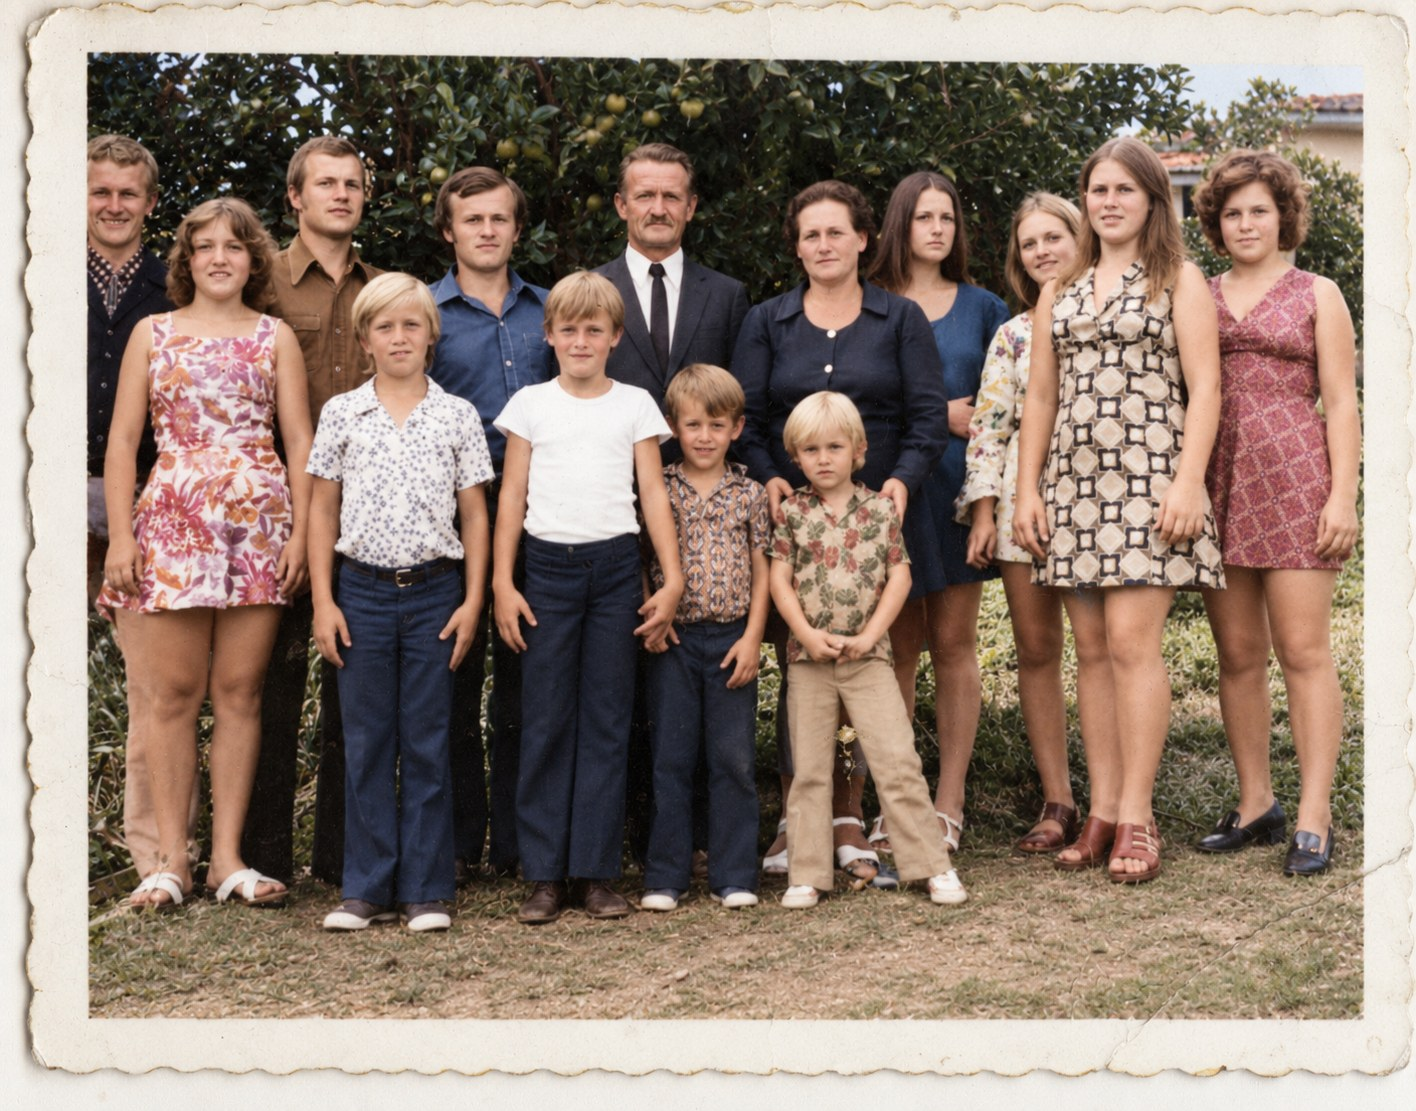
\includegraphics[width=0.85\linewidth,height=\textheight,keepaspectratio,alt={Baldoíno und Adelina mit ihren Kindern in Vidal Ramos, in den 1970er Jahren. Familienbesitz. Mit künstlicher Intelligenz restaurierte Fassung.}]{imagens/haas_baldoino_adelina_filhos_anos1970.jpg}
\caption{Baldoíno und Adelina mit ihren Kindern in Vidal Ramos, in den
1970er Jahren. Familienbesitz. Mit künstlicher Intelligenz restaurierte
Fassung.}
\end{figure}

Nun die Rechnung von der anderen Seite. Wäre das Paar in Sachsen\index[lugares]{sachsen@Sachsen}
geblieben, wäre Johann, 1914 dreißig Jahre alt, in den Ersten Weltkrieg
gezogen wie die Männer seines Alters. Wer zurückkam, erlebte die
Inflation von 1923, die Krise von 1929, den Nationalsozialismus und den
Zweiten Weltkrieg. Und das Vogtland\index[lugares]{vogtland@Vogtland}, wo die Familie der Mota\index[pessoas]{meier, maria@Meier, Maria} blieb,
wurde Teil der DDR: Die Briefe aus Rempesgrün\index[lugares]{rempesgrun@Rempesgrün} von 1971 kamen von hinter
der Mauer. In den deutschen Städten waren die Familien schon vor 1913
kleiner geworden. Um 1910 lag der Durchschnitt noch bei etwa vier
Kindern je Frau; in den 1930er Jahren war er unter zwei gefallen; nach
dem Krieg stieg er etwas an und fiel dann wieder. Heute liegt er bei
etwa 1,4. Im Hinterland von Santa Catarina blieben die Siedlerfamilien
noch ein halbes Jahrhundert lang groß: In Brasilien lag der Durchschnitt
1940 bei etwa sechs Kindern je Frau und 1970 noch nahe bei sechs. Eine
grobe Rechnung, nur um die Größenordnung zu sehen: Wären Johann und
Maria geblieben und hätten sie und ihre Nachkommen dem deutschen
Durchschnitt jeder Generation entsprochen, hätten sie heute einige
Dutzend Nachkommen, nicht sechshundert. Die Auswanderung hat eine
Familie nicht nur in die Ferne gebracht; sie hat sie vervielfacht.

Aber der Durchschnitt sagt nicht alles. Luisa\index[pessoas]{haas, luisa@Haas, Luisa} und Walter starben in Rio
do Ouro und hätten vielleicht überlebt, wären sie geblieben; Hildegard
und Frida starben in Deutschland, ganz ohne Reise. Die Mota\index[pessoas]{meier, maria@Meier, Maria} sah ihre
Eltern nie wieder, und von ihren Schwestern hörte sie fast sechzig Jahre
später nur durch Briefe. Wer bleibt, zahlt einen Preis, und wer geht,
zahlt einen anderen.

Und eine Ironie entgeht mir nicht. Die Welle, die einem Paar auf einem
Siedlerlos im Alto Vale zwölf Kinder brachte, ist auch hier
vorübergegangen. Brasilien hat heute weniger Kinder je Frau, als nötig
wären, um die Bevölkerung zu erhalten, etwa 1,6, und Santa Catarina noch
weniger. Ihr seid zwei, und ihr seid der Durchschnitt eurer Zeit, auf
beiden Seiten des Meeres. Was euch von den Vettern und Cousinen im
Vogtland\index[lugares]{vogtland@Vogtland} trennt, ist nicht mehr die Zahl der Geschwister.

Hat es sich also gelohnt? Für die Mota\index[pessoas]{meier, maria@Meier, Maria} kann ich nicht antworten, und ich
habe kein Recht, für sie zu antworten. Für mich kann ich antworten: Ich
lebe, weil sie gegangen sind. Und ihr beide lebt, weil 1913 zwei junge
Leute aus Chemnitz\index[lugares]{chemnitz@Chemnitz} in Marseille\index[lugares]{marseille@Marseille} an Bord gingen und weil 1939 Oma Dora\index[pessoas]{aenishaenslin, dora marta@Aenishaenslin, Dora Marta}
und Oscar darauf bestanden, wieder nach Brasilien zurückzufahren.
Zweimal, auf beiden Seiten der Familie, hat jemand beschlossen,
Deutschland zu verlassen. Wenn euch einmal jemand fragt, ob es sich
gelohnt hat, ist die ehrlichste Antwort vielleicht, das Foto der fünf
Generationen aufzuschlagen und die Gesichter zu zählen.

\section{Brief an Matheus und Lucas}\label{brief-an-matheus-und-lucas}

Matheus, Lucas.

Ich habe dieses Buch für euch geschrieben, und nun ist es Zeit zu sagen,
was ich seit dem Prolog sagen wollte.

Als ihr klein wart, habe ich euch beide manchmal am Tisch angeschaut und
mich gefragt, aus wie vielen Dörfern, Häfen, Handwerken und
Überlebenswundern zwei Jungen aus Santa Catarina im 21. Jahrhundert
gemacht sind. Jetzt weiß ich ein bisschen mehr. Ich weiß nicht alles.
Niemand weiß alles darüber, woher er kommt, und wer behauptet, es zu
wissen, erfindet. Aber ich weiß genug, um euch zu sagen, was ihr in euch
tragt.

Ihr tragt in euren Händen das Maurerlot und die Stuckkunst von Johann
Haas, dem Fata\index[pessoas]{haas, johann@Haas, Johann}, der in Ituporanga\index[lugares]{ituporanga@Ituporanga} Kirchen baute und Engel für die Gräber
armer Leute machte und heute in Aurora\index[lugares]{aurora@Aurora} zwischen den Engeln ruht, die er
selbst geformt hat. Ihr tragt die stille Sanftheit von Maria Meier\index[pessoas]{meier, maria@Meier, Maria}, der
Mota\index[pessoas]{meier, maria@Meier, Maria}, die nie Portugiesisch lernte und sich ihren Enkeln trotzdem
verständlich machte, mit einer langen Umarmung und einem blauen Blick.
Ihr tragt die Holzräder aus Heumaden\index[lugares]{heumaden@Heumaden}, die euer Urururgroßvater Michael
Meier und sein Sohn Adam für die Fuhrwerke der Oberpfalz\index[lugares]{oberpfalz@Oberpfalz} bauten, und den
eisernen Reifen, den der Schmied von Heumaden\index[lugares]{heumaden@Heumaden} um sie schmiedete. Ihr
tragt die Fabrikschicht des Arbeiters Josef Haas\index[pessoas]{haas, josef@Haas, Josef} in Leonberg\index[lugares]{leonberg@Leonberg}, der mit
zitternder Hand den Eintrag für den Sohn unterschrieb, der die Welt
durchqueren sollte.

Ihr tragt den Stahl der Solinger Schmieden der Doerner und der
Lauterjung. Ihr tragt den Mut eines sechsjährigen Jungen namens Anton
Michels, der 1828 in Desterro\index[lugares]{desterro@Desterro} an Land ging, in einem Land, das nicht auf
ihn wartete. Ihr tragt die fast hundertjährige Lebenskraft von Angela
Catharina Arns, die in einer Moselschleife geboren wurde und in Vargem
do Cedro starb, wenige Monate nachdem Opa Baldoíno zur Welt gekommen
war. Ihr tragt den katholischen Glauben der Haas, der Meier und der
Doerner und den lutherischen Glauben der Lohmann und der Hoeveler, die
einmal eine Grenze waren und die in eurem Haus am selben Tisch sitzen.

Und ihr tragt, auf der Seite eurer Mutter, die andere Hälfte, die ich
durch die Heirat kennen und lieben gelernt habe wie meine eigene: das
Licht, die Musik und die Herzlichkeit der Funke und der Hoeveler; die
Medizin von Großvater Carlos Heinz, nach dem in Pirabeiraba\index[lugares]{pirabeiraba@Pirabeiraba} eine Schule
und ein Gesundheitsposten benannt sind; die Klassenzimmer von Opa Erno\index[pessoas]{hoeveler, erno@Hoeveler, Erno}
in Estrela\index[lugares]{estrela@Estrela} und Nova Petrópolis\index[lugares]{nova petropolis@Nova Petrópolis}; die Beharrlichkeit der Lohmann, der
Schnack und der Endres im Vale do Taquari, in einem Haus an einem Fluss,
der 2024 wieder gestiegen ist; den zweiten Vornamen von Miguelina,
\emph{Leocádia}, der an Großmutter Ilusca weiterging, wie man einen Ring
weitergibt.

Ihr tragt auch die Verluste. Hildegard und Frida, die in Deutschland
starben, noch vor jeder Reise. Luisa\index[pessoas]{haas, luisa@Haas, Luisa} und Walter, die mit zwei Jahren und
mit einem Jahr in Marseille\index[lugares]{marseille@Marseille} an Bord gingen, lebend in Rio ankamen und
klein in Rio do Ouro\index[lugares]{rio do ouro@Rio do Ouro} starben. Den kleinen João von 1932. Suzana Regina
Schnack, die sechsundzwanzig Tage nach der Geburt eures Ururgroßvaters
Francisco starb. Als ich 2012 mit euch an meiner Seite in Laguna\index[lugares]{laguna@Laguna} war,
dachte ich daran, dass ihr ungefähr im Alter derer wart, die nicht groß
wurden. Ich denke wieder daran, jedes Mal, wenn ich die Zeile Nummer 36
in Moosbach\index[lugares]{moosbach@Moosbach} ansehe. Jeder von uns lebt, weil irgendwann jemand einen
Winter, eine Überfahrt, ein Fieber überlebt hat. Das schulden wir ihnen.

Und ihr tragt schließlich die Flüsse. Den Tubarão\index[lugares]{tubarao@Tubarão}, den Itajaí\index[lugares]{itajai@Itajaí}, den
Taquari. Unsere Vorfahren bauten ihre Häuser ans Wasser, weil das Wasser
Straße war und Kraft und guter Boden, und sie wussten nicht, wozu die
Flüsse fähig waren. Wir wissen es. Das ist einer der wenigen Vorteile,
die wir ihnen gegenüber haben: Wir messen, wir modellieren, wir sagen
vorher. Nutzt das. Wo immer ihr eure Häuser baut, schaut vorher auf den
Fluss.

Und jetzt meine Bitte.

Ich bitte euch, zu Ende zu bringen, was ich nicht zu Ende gebracht habe.
Es gibt ein Trauungsbuch in Eibenstock\index[lugares]{eibenstock@Eibenstock} in Sachsen\index[lugares]{sachsen@Sachsen}, das niemand aus der
Familie aufgeschlagen hat. Es gibt die Bücher der Hospedaria da Ilha das
Flores im Arquivo Nacional, die sagen werden, auf welchem Weg die
Familie nach Santa Catarina kam. Es gibt Sterbebücher in Anitápolis\index[lugares]{anitapolis@Anitápolis} und
das Friedhofsregister von Ituporanga\index[lugares]{ituporanga@Ituporanga}, die die Daten von Luisa\index[pessoas]{haas, luisa@Haas, Luisa} und Walter
bewahren. Es gibt, in irgendeinem Standesamt oder Pfarramt, die Geburt
von Tante Gertrudes. Es gibt einen Trauungseintrag in Burgtreswitz\index[lugares]{burgtreswitz@Burgtreswitz}, der
vielleicht erklärt, wer Katharina Reichenberger war. Es gibt den wahren
Ort und das wahre Jahr der Geburt von Ignazia Loch\index[pessoas]{loch, ignazia@Loch, Ignazia}. Es gibt so vieles.
Ein Stammbaum ist nie fertig, so wie eine Wettervorhersage nie die
letzte ist: Es kommt immer eine neue Beobachtung.

Ich bitte euch um etwas Schwierigeres. In Maxhütte-Haidhof\index[lugares]{maxhutte-haidhof@Maxhütte-Haidhof} erfuhr ich im
Februar 2018, dass dort ein Haas lebte, 1941 in Leonberg\index[lugares]{leonberg@Leonberg} geboren. Seinen
Namen habe ich in diesem Buch nicht geschrieben, und ich werde es auch
nicht tun. Er hat ein Recht auf sein Leben, und Gesetz und gesunder
Menschenverstand schützen dieses Recht. Aber die Tür ist noch da. Wenn
ihr eines Tages wollt, mit Respekt, mit Sorgfalt, mit der Geduld, die
man einem Fremden schuldet, der vielleicht zur Familie gehört, könnt ihr
einen Brief schreiben. Vielleicht antwortet er. Vielleicht ist er nicht
mehr dort; die Nachbarn sagten, ein Haas gleichen Namens sei gestorben
und seine Töchter lebten in Österreich. Vielleicht ist er gar nicht
verwandt. Und es gibt die Adresse aus den Briefen, die die Familie
aufbewahrt hat, in Falkenstein\index[lugares]{falkenstein@Falkenstein} im Vogtland\index[lugares]{vogtland@Vogtland}, wohin man ebenfalls
schreiben kann. Die Frage, die dieses Buch angetrieben hat, \emph{gibt
es auf der anderen Seite noch jemanden?}, verdient es, wenigstens einmal
laut gestellt zu werden. Ich habe sie schriftlich gestellt, in diesem
Buch. Die Stimme kann eure sein.

Ich bitte euch nicht, Familienforscher zu werden. Werdet, was ihr wollt.
Der Text zur Hundertjahrfeier endet mit einer Aufzählung dessen, was aus
den Nachkommen von Johann und Maria geworden ist (Mütter und Väter,
Bauern, Maurer, Lehrer, Köche, Ärzte, Ingenieure, Schreiner, Anwälte,
Wissenschaftler, Künstler), und kommt zu dem Schluss, dass wir alle,
wenn uns ausmacht, was wir sind, Menschen sind, so gewöhnlich und so
besonders wie sie. Ich stimme Marise\index[pessoas]{lourenco, marise haas@Lourenço, Marise Haas} zu. Ihr müsst die Vergangenheit
nicht als Last tragen. Es genügt, sie wie einen Kompass zu tragen: ein
kleines Ding, das in die Tasche passt und einem sagt, woher man kommt,
wenn man entscheiden muss, wohin man geht.

Wenn wir in meinem Beruf wissen wollen, woher eine Luftmasse kam,
berechnen wir eine Rückwärtstrajektorie: Wir gehen von dem Punkt aus, an
dem sie sich befindet, und berechnen den Weg rückwärts, Stunde um
Stunde, bis zum Ursprung. Dieses ganze Buch war eine
Rückwärtstrajektorie. Ich bin von euch in Florianópolis\index[lugares]{florianopolis@Florianópolis} ausgegangen und
Schritt für Schritt zurückgegangen, bis zu einem Hüttenwerk in Sandberg\index[lugares]{sandberg@Sandberg},
einer Heuwiese in Heumaden\index[lugares]{heumaden@Heumaden}, einer Schmiede in Solingen\index[lugares]{solingen@Solingen}, einer
Moselschleife. Jetzt, da ich am Ende angekommen bin, gebe ich euch das
Modell, damit ihr es in die andere Richtung laufen lasst. Vorwärts.
Dorthin, wohin ich nicht gehen kann.

Das vorletzte Bild, das ich euch hinterlasse, ist dieses. Auf dem
Friedhof von Aurora\index[lugares]{aurora@Aurora} im Alto Vale do Itajaí\index[lugares]{itajai@Itajaí} gibt es Gräber mit
Gipsengeln, gemacht von einem in Leonberg\index[lugares]{leonberg@Leonberg} geborenen Grabsteinmacher, der
1913 mit seiner Frau, zwei kleinen Kindern und fast nichts im Gepäck
nach Brasilien kam. Er liegt dort begraben, neben ihr, zwischen den
Engeln, die er für andere geformt hat. Die Engel tragen keinen Namen.
Soweit ich weiß, hat er sie nicht signiert. Aber wer zu schauen weiß,
erkennt die Hand.

Das letzte Bild ist eine Karte von Sachsen\index[lugares]{sachsen@Sachsen} um 1910. Glauchau\index[lugares]{glauchau@Glauchau} und
Chemnitz\index[lugares]{chemnitz@Chemnitz} liegen nur wenige Dutzend Kilometer voneinander entfernt. In
Glauchau\index[lugares]{glauchau@Glauchau} wird, laut den Einträgen bei FamilySearch, 1910 Oscar Martin
Funke geboren, der Großvater von Bárbara. In Chemnitz\index[lugares]{chemnitz@Chemnitz} wohnen, nach der
Erinnerung der Familie, Johann und Maria Haas, die 1913 aufbrechen. Kein
Papier sagt, dass sich ihre Wege kreuzten, und am wahrscheinlichsten
ist, dass sie nie voneinander wussten.

Danach geht jede Linie ihren Weg. Die Haas ziehen über Marseille\index[lugares]{marseille@Marseille}, Rio de
Janeiro, Rio do Ouro\index[lugares]{rio do ouro@Rio do Ouro} und Ituporanga\index[lugares]{ituporanga@Ituporanga}, und der Jüngste der Männer, die
blieben, mein Vater, geht nach Vidal Ramos\index[lugares]{vidal ramos@Vidal Ramos}. Die Funke kommen nach
Joinville\index[lugares]{joinville@Joinville}, wo 1939 Oscars Sohn Carlos Heinz geboren wird. Auf der Seite
der Haas wie auf der Seite der Funke kommen noch die Mosel\index[lugares]{mosel@Mosel}, Solingen\index[lugares]{solingen@Solingen},
der Taquari und die Schweiz hinzu. Und am 30. September 1995 um sieben
Uhr abends heiratet in der Kirche der Evangelischen Gemeinde von
Florianópolis\index[lugares]{florianopolis@Florianópolis} ein Enkel von Johann eine Enkelin von Oscar,
zweiundachtzig Jahre nach der \emph{Formosa}. Die beiden Linien brachen
nahe beieinander auf und brauchten fast ein Jahrhundert, um sich auf der
anderen Seite des Meeres zu treffen. Aus dieser Begegnung seid ihr
geboren.

Ihr wisst jetzt zu schauen.

Der Kompass gehört euch.

In aller Liebe, euer Vater,

Reinaldo

\emph{Florianópolis\index[lugares]{florianopolis@Florianópolis}}

\chapter*{Anmerkung zu den Quellen und den offenen
Rätseln}\markboth{Anmerkung zu den Quellen und den offenen
Rätseln}{Anmerkung zu den Quellen und den offenen
Rätseln}\label{nota-fontes}
\addcontentsline{toc}{chapter}{Anmerkung zu den Quellen und den offenen
Rätseln}

Dieses Buch wurde aus Dokumenten, Erinnerungen und Zweifeln geschrieben,
in dieser Rangfolge des Vertrauens. Wenn ein Dokument und eine
Erinnerung einander widersprachen, habe ich mich an das Dokument
gehalten, und die Erinnerung wurde zur Frage. Wenn zwei Dokumente
einander widersprachen, habe ich beide sichtbar gelassen. Die
Rekonstruktionen (die Kälte einer Nacht in Heumaden\index[lugares]{heumaden@Heumaden}, der Laderaum eines
Schiffes, die Hütte im Wald von Rio Novo\index[lugares]{rio novo@Rio Novo}) sind im Text mit Wörtern wie
\emph{ich stelle mir vor}, \emph{wahrscheinlich}, \emph{man erzählt}
gekennzeichnet. Der Rest stammt aus den Papieren.

\section{Die wichtigsten Quellen}\label{die-wichtigsten-quellen}

Die Forschung lief auf drei Wegen. Der erste waren die Einträge bei
FamilySearch, die Indizes und, wo immer möglich, die Bilder der
Kirchenbücher und Standesamtsregister aus Brasilien und Deutschland. Der
zweite waren die Tauf-, Trauungs- und Sterbebücher der deutschen
katholischen Pfarreien, Seite für Seite gelesen mit Hilfe eines
KI-Assistenten, Antigravity, der die digitalisierten Bücher nach den
Namen durchsuchte. Der dritte war der Stammbaum meines Vetters Agenor\index[pessoas]{haas, agenor@Haas, Agenor}
Haas, den er über Jahre aufgebaut hat. Wo die drei voneinander
abweichen, gilt das Originaldokument mehr als der Index und der Index
mehr als der Stammbaum.

Für die Familie Haas sind die wichtigsten Quellen die zeitgenössischen
Dokumente: die Passagierliste des Dampfers \emph{Formosa}, die
standesamtlichen und kirchlichen Einträge und die Friedhofsregister.
Danach kommen die große genealogische Tabelle von Agenor\index[pessoas]{haas, agenor@Haas, Agenor} Haas und
schließlich der Text \emph{História de João e Maria Meyer Haas}, den
Marise\index[pessoas]{lourenco, marise haas@Lourenço, Marise Haas} Haas Lourenço für die Hundertjahrfeier am 30. März 2013
geschrieben hat. Dieser Text hat die Erinnerung der Familie gesammelt
und war der Ausgangspunkt der Forschung, irrt aber oft, wo er sich mit
Dokumenten vergleichen lässt. Er behauptet zum Beispiel, die
Ausschiffung in Rio sei verweigert worden, es habe an Bord viele
Todesfälle gegeben und Luisa\index[pessoas]{haas, luisa@Haas, Luisa} und Walter seien in den Baracken von Laguna\index[lugares]{laguna@Laguna}
gestorben. Die Bordliste und die Bestattungen widerlegen diese
Behauptungen. Deshalb gilt er in diesem Buch als Überlieferung, nicht
als Quelle. Zu den Dokumenten kommt das Abschiedsfoto \emph{„Zum
Andenken! vor unserer Abreise nach Brasilien, 7. März 1913''}; die
Passagierliste der \emph{Formosa} wurde am 26. März 1913 in Rio de
Janeiro unterzeichnet. Hinzu kommen die mündlichen Zeugnisse, die ich
selbst gehört habe: das meines Vaters Baldoíno über die Umbettung der
sterblichen Überreste seiner Geschwister von Anitápolis\index[lugares]{anitapolis@Anitápolis} nach Ituporanga\index[lugares]{ituporanga@Ituporanga}
und das meines Großvaters Fernando Dörner\index[pessoas]{dorner, fernando@Dörner, Fernando} über die Jahre in Vidal Ramos\index[lugares]{vidal ramos@Vidal Ramos}.
Außerdem der Eintrag Nr. 47 von 1884 im Standesamt Leonberg\index[lugares]{leonberg@Leonberg}, heute
Maxhütte-Haidhof\index[lugares]{maxhutte-haidhof@Maxhütte-Haidhof}; die Trauung von Joseph Haas und Franziska Dengler\index[pessoas]{dengler, franziska@Dengler, Franziska} 1878
in Leonberg\index[lugares]{leonberg@Leonberg}, die zeigte, dass die Taufe von 1847 in Stoffen\index[lugares]{stoffen@Stoffen}, auf die
sich die ersten Fassungen dieses Buches stützten, die eines
Namensvetters war; und vier Einträge aus den Pfarrbüchern von St.~Peter
und Paul in Moosbach\index[lugares]{moosbach@Moosbach} (1859, 1861, 1884 und 1888).

Für die Zweige Doerner, Preiss, Michels, Arns und Loch habe ich die bei
FamilySearch gesammelten Einträge verwendet und die Studien von Toni
Jochem und Mitarbeitern über die Kolonien São Pedro de Alcântara\index[lugares]{sao pedro de alcantara@São Pedro de Alcântara}, Santa
Isabel und Piedade. Dazu kommen die Volkszählung von 1920, das Bild des
Trauungseintrags von Carlos Dörner\index[pessoas]{dorner, carlos@Dörner, Carlos} und Hulda Peters von 1900 und die
Sterbeurkunden von Fernando Dörner\index[pessoas]{dorner, fernando@Dörner, Fernando} und Gertrudes Preiss\index[pessoas]{preiss, gertrudes@Preiss, Gertrudes} in Brusque\index[lugares]{brusque@Brusque}.

Für die Zweige von Bárbara (Lohmann, Schnack, Endres, Hoeveler und
Funke) habe ich das Fotoarchiv der Familie und die Einträge bei
FamilySearch verwendet. Hinzu kommen die Dossiers der CAPEF in Estrela\index[lugares]{estrela@Estrela}
über die Gründerfamilien und die Geschichte der Fazenda Lohmann in Roca
Sales. Schließlich gibt es die Zeitungsberichte und Ehrungen für
Dr.~Carlos Heinz Funke\index[pessoas]{funke, carlos heinz@Funke, Carlos Heinz} in Joinville\index[lugares]{joinville@Joinville} sowie das topographische und
hydrologische Profil der Casa Lohmann in Palmas\index[lugares]{palmas@Palmas}, Arroio do Meio\index[lugares]{arroio do meio@Arroio do Meio}.

Fast alle diese Materialien liegen im digitalen Repository des
Stammbaums, das dieses Buch begleitet. Ausgenommen sind die Materialien,
die Dritten gehören, und Agenors Tabelle, die Daten lebender Verwandter
enthält und im privaten Familienarchiv bleibt. Im Repository liegt auch
die vollständige Liste der noch offenen Fragen, mit den Archiven, in
denen man nach jeder Antwort suchen kann
(\texttt{docs/questoes\_pesquisa\_antigravity.md}). Die Antworten auf
diese Fragen, mit Hilfe eines Forschungsassistenten zusammengetragen,
stehen in \texttt{docs/respostas\_pesquisa\_antigravity.md}. Davon habe
ich nur verwendet, was ich in den Einträgen bei FamilySearch oder in den
Bildern selbst nachprüfen konnte. Beim Nachprüfen fand ich auch Lesungen
von Urkunden mit Einzelheiten, die das Bild nicht enthält, etwa die
Uhrzeit und den Arzt beim Tod von Gertrudes Preiss\index[pessoas]{preiss, gertrudes@Preiss, Gertrudes}, die mit denen des
benachbarten Eintrags vertauscht waren. Deshalb ist jenes Dokument als
Karte von Spuren zu lesen, nicht als Quelle.

\section{Rätsel, die der nächsten Generation
bleiben}\label{ruxe4tsel-die-der-nuxe4chsten-generation-bleiben}

\textbf{Gertrudes.} Zum Teil gelöst: Sie wurde am 23. November 1913 in
Teresópolis getauft, als Tochter von Johann Haas\index[pessoas]{haas, johann@Haas, Johann} und Maria Meyer, und
ihr Profil nennt als Geburt den 5. Mai 1913 in Anitápolis\index[lugares]{anitapolis@Anitápolis}. Es fehlt die
Geburtsurkunde, die den Ort festlegen würde.

\textbf{Luisa\index[pessoas]{haas, luisa@Haas, Luisa} und Walter.} Sie kamen lebend in Rio an und starben in Rio
do Ouro, Anitápolis\index[lugares]{anitapolis@Anitápolis}. Jahre später holten ihre Geschwister die
sterblichen Überreste nach Ituporanga\index[lugares]{ituporanga@Ituporanga}, wo Walter begraben ist. Es fehlen
die Daten der Tode und der Umbettung.

\textbf{Wo die Familie nach Santa Catarina kam.} Laguna\index[lugares]{laguna@Laguna}, laut
Überlieferung; Florianópolis\index[lugares]{florianopolis@Florianópolis}, wo Agenor\index[pessoas]{haas, agenor@Haas, Agenor} gesucht hat und worauf die Taufe
von Gertrudes in Teresópolis hindeutet. Die Bücher der Hospedaria da
Ilha das Flores im Arquivo Nacional dürften es sagen.

\textbf{Die Daten der Reise.} Das Abschiedsfoto nennt den 7. März 1913,
und die Passagierliste wurde am 26. März in Rio unterzeichnet. Die
Tabelle verzeichnet die Abfahrt am 13. März und die Ankunft am 26.
April. Es fehlt auch der Eintrag über die Ankunft in Santa Catarina.

\textbf{Die Patin der Mota\index[pessoas]{meier, maria@Meier, Maria}.} Die Überlieferung spricht von der Tante
Katharina Meier, aber das Taufbuch von Moosbach\index[lugares]{moosbach@Moosbach} nennt \emph{Kath.
Reichenberger, Bäuerin von Burgtreswitz\index[lugares]{burgtreswitz@Burgtreswitz}}, und die Taufe am Tag der
Geburt.

\textbf{Eibenstock\index[lugares]{eibenstock@Eibenstock}.} Wie kamen ein Maurer aus Leonberg\index[lugares]{leonberg@Leonberg} und ein Mädchen
aus Heumaden\index[lugares]{heumaden@Heumaden} 1907 dazu, in einer sächsischen Stadt zu heiraten? Die
Familie erinnert sich, dass sie in Chemnitz\index[lugares]{chemnitz@Chemnitz} wohnten, als sie aufbrachen,
und hat Briefe aus Falkenstein\index[lugares]{falkenstein@Falkenstein} im Vogtland\index[lugares]{vogtland@Vogtland} aufbewahrt; Eibenstock\index[lugares]{eibenstock@Eibenstock} liegt
zwischen beiden Orten. Die Papiere, die antworten können, sind der
Heiratseintrag im Standesamt Eibenstock\index[lugares]{eibenstock@Eibenstock} und, falls die ersten Kinder in
Sachsen\index[lugares]{sachsen@Sachsen} geboren wurden, die Geburts- und Sterbeeinträge in Chemnitz\index[lugares]{chemnitz@Chemnitz}. Die
Briefe aus Rempesgrün\index[lugares]{rempesgrun@Rempesgrün} (1971 bis 1974), geschrieben von einer mit Walter
Heckel verheirateten Schwester der Mota\index[pessoas]{meier, maria@Meier, Maria}, zeigen, dass die Familie Meier
schließlich im Vogtland\index[lugares]{vogtland@Vogtland} landete, und das Taufbuch von Moosbach\index[lugares]{moosbach@Moosbach}
verzeichnet nach 1892 nichts mehr von ihr. Wann sie umzogen, ist noch
offen.

\textbf{Die Briefe aus Rempesgrün\index[lugares]{rempesgrun@Rempesgrün}.} Es sind vier Briefe und vier
Umschläge aus der DDR, im November 2026 digitalisiert. Antigravity hat
sie transkribiert und übersetzt; ich habe den sichtbaren Text jedes
Briefes an den Bildern geprüft. Die Wörter in eckigen Klammern in
Kapitel 7 markieren Zeilenenden, die der Scanner abgeschnitten hat. Das
Jahr 1974 beim dritten Brief stammt vom Eingangsstempel des Umschlags in
Aurora\index[lugares]{aurora@Aurora} und davon, dass er von den Eltern als bereits verstorben spricht.
Der zweite und der vierte Brief tragen kein sichtbares Datum.

\textbf{Die Eltern von Josef Haas\index[pessoas]{haas, josef@Haas, Josef}.} Die ersten Fassungen dieses Buches
gaben Josef, kollaborativen Stammbäumen folgend, als 1847 in Stoffen\index[lugares]{stoffen@Stoffen}
geboren an, Sohn von Georg Haas und Maria Anna Albrecht. Die Trauung von
1878 in Leonberg\index[lugares]{leonberg@Leonberg} (\texttt{Leonberg\_Bul012}, S. 8, Nr. 4), die ich am
Bild geprüft habe, nennt als Eltern \emph{Mich. Haas} und
\emph{Kunigunde Stadelmann\index[pessoas]{stadelmann, kunigunde@Stadelmann, Kunigunde}}. Ihre Herkunft aus Etzgersrieth\index[lugares]{etzgersrieth@Etzgersrieth}, die
Geschwister von Johann und das Datum 8. Juli 1884 bei der Taufe stammen
aus der Lesung von Antigravity und müssen noch geprüft werden.

\textbf{Die Geschwister der Mota\index[pessoas]{meier, maria@Meier, Maria}.} Das Taufbuch von Moosbach\index[lugares]{moosbach@Moosbach} nennt als
Kinder von Georg Adam Meier\index[pessoas]{meier, georg adam@Meier, Georg Adam} und Franziska Voit\index[pessoas]{voit, franziska@Voit, Franziska} Maria Katharina (1886),
Maria (1888), Theresia\index[pessoas]{meier, theresia@Meier, Theresia} (1891) und Michael (1893). Die Taufen von Maria
und Theresia\index[pessoas]{meier, theresia@Meier, Theresia} habe ich am Bild geprüft; die anderen sind Lesungen von
Antigravity. Nach der zweiten Lesung ist der Beruf des Vaters 1888
\emph{Krämer} und nicht \emph{Ökonom}, wie ich früher las. Dieselbe
Lesung gab Johann Haas\index[pessoas]{haas, johann@Haas, Johann}' Geburt mit dem 8. Juli 1884 an; ich habe den
Eintrag Nr. 47 geprüft, und dort steht ausgeschrieben \emph{elf},
eingetragen am 13. Juli. Die Geschwister, die die kollaborativen
Stammbäume Maria zuschreiben (Johann Baptist, Barbara, Margaretha,
Josef, Georg, Anna), erscheinen dort nicht.

\textbf{Ignazia Loch\index[pessoas]{loch, ignazia@Loch, Ignazia}.} Das Datum 1828 in São Pedro de Alcântara\index[lugares]{sao pedro de alcantara@São Pedro de Alcântara} liegt
vor der Gründung der Kolonie und muss deshalb ein Näherungswert sein.

\textbf{Der Fata\index[pessoas]{haas, johann@Haas, Johann} als „Presbyter''.} In der katholischen Tradition ist
ein Presbyter ein Priester. Am wahrscheinlichsten war der Fata\index[pessoas]{haas, johann@Haas, Johann}
Kirchenpfleger oder Mitglied im Vorstand der Kapelle. Das Livro do
Tombo, die Pfarrchronik von Ituporanga\index[lugares]{ituporanga@Ituporanga}, dürfte es sagen, ebenso die
Daten der Kirchen, des Pfarrhauses, des Seminars und des Krankenhauses,
an denen die Haas gearbeitet haben.

\textbf{Die Trauung von 1900.} Das Bild des Eintrags und eine alte, in
der Familie umlaufende Abschrift weichen beim Zelebranten, bei den
Trauzeugen und bei einer angeblichen Dispens wegen gemischter Religion
voneinander ab. Es gilt das Bild: eine katholische Trauung ohne Dispens.
Die alte Abschrift hat kein Dokument hinter sich und wurde verworfen.
Der Akt vom 28.04.1900, den ich Hulda Peters zuschrieb, ist bei der
Prüfung die Taufe der Tochter Joanna von 1902. Die Doerner waren
katholisch.

\textbf{Carlos Doerner.} FamilySearch fasst in einem einzigen Profil
(„Carl Reinhard Dörner'', Solingen\index[lugares]{solingen@Solingen}, 1854) drei oder vier Männer
zusammen: Carlos, der zwei Geburtsurkunden hatte; seinen Sohn Carlos
Reinaldo (1882--1953); und einen Namensvetter, der 1893 in Águas Mornas\index[lugares]{aguas mornas@Águas Mornas}
Charlotte Elisabetha Stock heiratete, vielleicht ein Vetter. Sicher ist,
was aus dem Eintrag von 1900 hervorgeht: Sohn von Guilherme Dörner\index[pessoas]{dorner, guilherme@Dörner, Guilherme} und
Joanna Lauterjung\index[pessoas]{lauterjung, joanna@Lauterjung, Joanna}, um 1854 in Europa geboren. Die Kinder aus der zweiten
Ehe, an die sich die Familie erinnert (Laura, Clara, Carlos Júnior, Ida,
Ricardo), stimmen nicht mit denen in den Indizes überein (Bertha,
Joanna, Emma, João, Gustavo, Martinho).

\textbf{Anna Eller\index[pessoas]{eller, anna@Eller, Anna}.} Die Geburt „1858 in Rio Grande do Sul'' ist eine
von FamilySearch erzeugte Angabe ohne Quelle. Ihre Geschwister wurden in
Deutschland (1860) und in São Bonifácio\index[lugares]{sao bonifacio@São Bonifácio} (1866 und 1869) geboren. Ihre
Taufe fehlt.

\textbf{Fernando Dörner\index[pessoas]{dorner, fernando@Dörner, Fernando} in Vidal Ramos\index[lugares]{vidal ramos@Vidal Ramos}.} Die Einträge der Kinder
verorten die Familie von 1929 oder 1930 bis mindestens 1948 in Vidal
Ramos. Das Porträt, das Fábio Sidney Thiesen für das \emph{Jornal Mirim}
(2011) schrieb, nennt die Ankunft im Mai 1927, das Sägewerk in Santa
Cruz, den Laden im Ortskern, die Zeit als Polizeikommissar und den Umzug
nach Brusque\index[lugares]{brusque@Brusque} 1964. Die Unterstützung für Hitler und die Reue sind sein
Zeugnis mir gegenüber, ohne Dokument. Die Milizen, an denen er teilnahm,
Jahr und Kompanie des Landkonflikts, in dem er sich gegen die anderen
Kolonisten stellte, und die Namen der Gefangenen sind noch nicht belegt.
Wenn es die portugiesischsprachigen \emph{Seleções} waren, die ihn die
Seite wechseln ließen, dann fand der Wechsel 1942 oder später statt. Die
Akten der politischen Polizei von Santa Catarina liegen im Arquivo
Público do Estado, und von ihm gibt es eine einzige Fotografie, um 1927,
mit Gertrudes und den Töchtern Hilda Ana und Adelina.

\textbf{Die zwölf Kinder von Francisco Jacob Lohmann\index[pessoas]{lohmann, francisco jacob@Lohmann, Francisco Jacob}.} Die Geburtsdaten
und die Schreibweisen der Namen passen nicht zusammen.

\textbf{Der Haas aus Leonberg\index[lugares]{leonberg@Leonberg}.} Ein 1941 in Leonberg geborener Mann
erschien 2018 in den Unterlagen der Stadt mit dem Familiennamen des
\emph{Fata\index[pessoas]{haas, johann@Haas, Johann}}. Beim Besuch widersprachen sich die Auskünfte: Eine Person
sagte, der Vetter meines Vaters lebe; die Nachbarn, er sei gestorben und
seine Töchter lebten in Österreich. Die Verwandtschaft ist
wahrscheinlich, aber nicht nachgewiesen. Dieses Buch ist auch ein
möglicher Brief an ihn.

\section{Papiere, die noch
hinzukommen}\label{papiere-die-noch-hinzukommen}

Die Briefe, die die Schwester unserer Mota\index[pessoas]{meier, maria@Meier, Maria} (Maria Meier Haas), Theresia\index[pessoas]{meier, theresia@Meier, Theresia}
Meier, und Walter Heckel\index[pessoas]{heckel, walter@Heckel, Walter} aus Deutschland schickten und die so lange in
einer Schublade vergessen lagen, sind inzwischen gelesen; ihr findet sie
in Kapitel 7. Zwei Schätze der Familie fehlen noch: das Buch über die
Ankunft der Funke in Brasilien und der Brief, in dem Oma Adelina über
ihre Kinder schrieb und den Tante Marise\index[pessoas]{lourenco, marise haas@Lourenço, Marise Haas} aufbewahrt. Was sie erzählen,
kann berichtigen, was hier steht.

Berichtigungen, Fotografien und Erinnerungen sind willkommen. Der
Stammbaum wird nie fertig; er wechselt nur die Hände.

\chapter*{Die Stammbäume der Familie}\markboth{Die Stammbäume der Familie}{Die Stammbäume der Familie}\label{arvores}
\addcontentsline{toc}{chapter}{Die Stammbäume der Familie}

Dies sind eure Stammbäume bis zur siebten Generation, so weit ich sie
heute kenne, mit den Daten von Geburt, Tod, Heirat und Ankunft in
Brasilien. Beginnt mit Baum 1, der von euch bis zu den Urgroßeltern
reicht, und folgt den Hinweisen „continua na árvore'': Jeder der anderen
Bäume ist ein Zweig der Familie, bis zur siebten Generation. Das
Heiratsdatum der Eltern einer Person steht in ihrem eigenen Kästchen,
rot, nach „pais ∞``. Wer nicht erscheint, ist mir noch unbekannt; „pais
a descobrir'' ist die Frage, die ich euch hinterlasse.

Die Baumdiagramme sind portugiesisch beschriftet: „n.'' bedeutet
geboren, „bat.'' getauft, „†'' gestorben, „chegou'' angekommen, „pais
∞'' Heirat der Eltern, „continua na árvore N'' Fortsetzung in Baum N und
„pais a descobrir'' Eltern noch unbekannt. Ein guter Teil der älteren
Daten stammt von FamilySearch, einem kollaborativen Stammbaum, und muss
noch in den Büchern nachgeprüft werden. Lebende Personen erscheinen nur
mit dem Jahr oder ohne Datum.

\begin{paisagem}

\begin{figure}
\centering
\includegraphics[width=1\linewidth,height=0.88\textheight,alt={Matheus und Lucas, bis zu den Urgroßeltern.}]{imagens/arvore_01.jpg}
\caption{Matheus und Lucas, bis zu den Urgroßeltern.}
\end{figure}

\end{paisagem}

\begin{paisagem}

\begin{figure}
\centering
\includegraphics[width=1\linewidth,height=0.88\textheight,alt={Vorfahren von Johann Haas und Maria Meier, dem Fata und der Mota.}]{imagens/arvore_02.jpg}
\caption{Vorfahren von Johann Haas und Maria Meier, dem Fata und der
Mota\index[pessoas]{meier, maria@Meier, Maria}.}
\end{figure}

\end{paisagem}

\begin{paisagem}

\begin{figure}
\centering
\includegraphics[width=1\linewidth,height=0.88\textheight,alt={Vorfahren von Fernando Dörner, dem Opapa.}]{imagens/arvore_03.jpg}
\caption{Vorfahren von Fernando Dörner, dem Opapa.}
\end{figure}

\end{paisagem}

\begin{paisagem}

\begin{figure}
\centering
\includegraphics[width=1\linewidth,height=0.88\textheight,alt={Vater der Omama: Vorfahren von Emanuel Preis.}]{imagens/arvore_04.jpg}
\caption{Vater der Omama: Vorfahren von Emanuel Preis.}
\end{figure}

\end{paisagem}

\begin{paisagem}

\begin{figure}
\centering
\includegraphics[width=1\linewidth,height=0.88\textheight,alt={Mutter der Omama: Vorfahren von Helena Michels.}]{imagens/arvore_05.jpg}
\caption{Mutter der Omama: Vorfahren von Helena Michels.}
\end{figure}

\end{paisagem}

\begin{paisagem}

\begin{figure}
\centering
\includegraphics[width=1\linewidth,height=0.88\textheight,alt={Vorfahren von Oscar Martin Funke.}]{imagens/arvore_06.jpg}
\caption{Vorfahren von Oscar Martin Funke.}
\end{figure}

\end{paisagem}

\begin{paisagem}

\begin{figure}
\centering
\includegraphics[width=1\linewidth,height=0.88\textheight,alt={Vorfahren von Dora Marta Aenishaenslin, der Oma Dora.}]{imagens/arvore_07.jpg}
\caption{Vorfahren von Dora Marta Aenishaenslin, der Oma Dora.}
\end{figure}

\end{paisagem}

\begin{paisagem}

\begin{figure}
\centering
\includegraphics[width=1\linewidth,height=0.88\textheight,alt={Vorfahren von Erno Hoeveler.}]{imagens/arvore_08.jpg}
\caption{Vorfahren von Erno Hoeveler.}
\end{figure}

\end{paisagem}

\begin{paisagem}

\begin{figure}
\centering
\includegraphics[width=1\linewidth,height=0.88\textheight,alt={Eltern der Oma Rosita: Vorfahren von Francisco Jacob Lohmann und Miguelina Leocádia Endres.}]{imagens/arvore_09.jpg}
\caption{Eltern der Oma Rosita: Vorfahren von Francisco Jacob Lohmann
und Miguelina Leocádia Endres\index[pessoas]{endres, miguelina leocadia@Endres, Miguelina Leocádia}.}
\end{figure}

\end{paisagem}

\backmatter
\cleardoublepage
\printindex[pessoas]
\printindex[lugares]
\end{document}
